\documentclass[twoside]{book}

% Packages required by doxygen
\usepackage{calc}
\usepackage{doxygen}
\usepackage{graphicx}
\usepackage[utf8]{inputenc}
\usepackage{makeidx}
\usepackage{multicol}
\usepackage{multirow}
\usepackage{textcomp}
\usepackage[table]{xcolor}

% Font selection
\usepackage[T1]{fontenc}
\usepackage{mathptmx}
\usepackage[scaled=.90]{helvet}
\usepackage{courier}
\usepackage{amssymb}
\usepackage{sectsty}
\renewcommand{\familydefault}{\sfdefault}
\allsectionsfont{%
  \fontseries{bc}\selectfont%
  \color{darkgray}%
}
\renewcommand{\DoxyLabelFont}{%
  \fontseries{bc}\selectfont%
  \color{darkgray}%
}

% Page & text layout
\usepackage{geometry}
\geometry{%
  a4paper,%
  top=2.5cm,%
  bottom=2.5cm,%
  left=2.5cm,%
  right=2.5cm%
}
\tolerance=750
\hfuzz=15pt
\hbadness=750
\setlength{\emergencystretch}{15pt}
\setlength{\parindent}{0cm}
\setlength{\parskip}{0.2cm}
\makeatletter
\renewcommand{\paragraph}{%
  \@startsection{paragraph}{4}{0ex}{-1.0ex}{1.0ex}{%
    \normalfont\normalsize\bfseries\SS@parafont%
  }%
}
\renewcommand{\subparagraph}{%
  \@startsection{subparagraph}{5}{0ex}{-1.0ex}{1.0ex}{%
    \normalfont\normalsize\bfseries\SS@subparafont%
  }%
}
\makeatother

% Headers & footers
\usepackage{fancyhdr}
\pagestyle{fancyplain}
\fancyhead[LE]{\fancyplain{}{\bfseries\thepage}}
\fancyhead[CE]{\fancyplain{}{}}
\fancyhead[RE]{\fancyplain{}{\bfseries\leftmark}}
\fancyhead[LO]{\fancyplain{}{\bfseries\rightmark}}
\fancyhead[CO]{\fancyplain{}{}}
\fancyhead[RO]{\fancyplain{}{\bfseries\thepage}}
\fancyfoot[LE]{\fancyplain{}{}}
\fancyfoot[CE]{\fancyplain{}{}}
\fancyfoot[RE]{\fancyplain{}{\bfseries\scriptsize Generated on Tue Dec 2 2014 00\-:48\-:01 for S\-M\-A by Doxygen }}
\fancyfoot[LO]{\fancyplain{}{\bfseries\scriptsize Generated on Tue Dec 2 2014 00\-:48\-:01 for S\-M\-A by Doxygen }}
\fancyfoot[CO]{\fancyplain{}{}}
\fancyfoot[RO]{\fancyplain{}{}}
\renewcommand{\footrulewidth}{0.4pt}
\renewcommand{\chaptermark}[1]{%
  \markboth{#1}{}%
}
\renewcommand{\sectionmark}[1]{%
  \markright{\thesection\ #1}%
}

% Indices & bibliography
\usepackage{natbib}
\usepackage[titles]{tocloft}
\setcounter{tocdepth}{3}
\setcounter{secnumdepth}{5}
\makeindex

% Hyperlinks (required, but should be loaded last)
\usepackage{ifpdf}
\ifpdf
  \usepackage[pdftex,pagebackref=true]{hyperref}
\else
  \usepackage[ps2pdf,pagebackref=true]{hyperref}
\fi
\hypersetup{%
  colorlinks=true,%
  linkcolor=blue,%
  citecolor=blue,%
  unicode%
}

% Custom commands
\newcommand{\clearemptydoublepage}{%
  \newpage{\pagestyle{empty}\cleardoublepage}%
}


%===== C O N T E N T S =====

\begin{document}

% Titlepage & ToC
\hypersetup{pageanchor=false}
\pagenumbering{roman}
\begin{titlepage}
\vspace*{7cm}
\begin{center}%
{\Large S\-M\-A }\\
\vspace*{1cm}
{\large Generated by Doxygen 1.8.6}\\
\vspace*{0.5cm}
{\small Tue Dec 2 2014 00:48:01}\\
\end{center}
\end{titlepage}
\clearemptydoublepage
\tableofcontents
\clearemptydoublepage
\pagenumbering{arabic}
\hypersetup{pageanchor=true}

%--- Begin generated contents ---
\chapter{R\-E\-A\-D\-M\-E}
\label{md_ns3_README}
\hypertarget{md_ns3_README}{}
{\ttfamily include/ns3/} and {\ttfamily lib/} should be symlinked to the N\-S3 build directory where N\-S3 builds the shared libraries and outputs the headers for the modules its built with.

{\ttfamily include/} will be added to the system include path and {\ttfamily lib/} to the library search path for targets in this project. Source depending on N\-S3 can therefore include its headers as if they were in the system path\-: \begin{DoxyVerb}#include <ns3/xxxx.h>
\end{DoxyVerb}


This means that N\-S3 needs to be built before any source depending on it or those headers won't be found.

If N\-S3 is moved or the version changed then the symlinks need to be updated. 
\chapter{Building}
\label{md_README}
\hypertarget{md_README}{}
Configure the makefile by invoking {\ttfamily cmake} in the build directory. Do not invoke {\ttfamily cmake} in any component's root directory or any other path. \begin{DoxyVerb} # -DCMAKE_BUILD_TYPE=Debug - attach symbols to the output (on by default)
 # -Dbuild_tests=OFF        - don't build test executables

 cd core/build/
 cmake ../
 make
 ./libsma_test
\end{DoxyVerb}


Project sources are declared in {\ttfamily C\-Make\-Lists.\-txt}.

\subsection*{Testing}

Using gtest\-: \begin{DoxyVerb}test/test1.hh
------------------
#pragma once

#include "log.hh"
#include "gtest/gtest.h"

TEST(MyClass, it_does_x_correctly)
{
  LOG(DEBUG) << "Hello!";
  ASSERT_EQ(1, 1);
  ASSERT_GT(1, 0);
  LOG(FATAL) << "Something terrible happened";
}

test/test_main.cc
------------------
/**************************************************************************
 * This file just creates a compilation unit with the tests.

#include "log.hh"
// Must come first and only once in application 
_INITIALIZE_EASYLOGGINGPP

#include "test1.hh"
// more tests

#include "gtest/gtest.h"

int main(int argc, char** argv)
{
  // Allow command line arguments to specify tests
  ::testing::InitGoogleTest(&argc, argv);

  // Trim down some noisy output
  // Optionally turn logging off or change debug level (default ALL)
  el::Loggers::reconfigureAllLoggers(
    el::ConfigurationType::Format,
    "%datetime{%m:%s.%g} %levshort [%thread] %func (%fbase:%line) %msg");

  return RUN_ALL_TESTS();
}
\end{DoxyVerb}


\subsection*{Project Setup}

\subsubsection*{Using C++11}

\paragraph*{N\-S-\/3 via {\ttfamily wscript}}

\begin{DoxyVerb}def build(bld):
  obj = bld.create_ns3_program('ex', ['csma', 'internet', 'applications'])
  obj.cxxflags = ['-std=c++11']
  obj.source = ['ex.cc']
\end{DoxyVerb}


Compile and run by changing into the {\ttfamily ns-\/3.\-xx/build} directory and running {\ttfamily ./waf -\/-\/run example}

\paragraph*{Android}

\begin{quotation}
If you're using command line N\-D\-K support this is what I had to put in my {\ttfamily jni/\-Application.\-mk} to get C++11 support with A\-P\-I 19

\end{quotation}


(\href{http://stackoverflow.com/a/21386866}{\tt stackoverflow}) \begin{DoxyVerb}NDK_TOOLCHAIN_VERSION := 4.8
# APP_STL := stlport_shared  --> does not seem to contain C++11 features
APP_STL := gnustl_shared

# Enable c++11 extentions in source code
APP_CPPFLAGS += -std=c++11
\end{DoxyVerb}


\subsection*{Protocols}

\subsubsection*{Content dissemination}


\begin{DoxyEnumerate}
\item Interest a. Announcement a. Replication
\end{DoxyEnumerate}
\begin{DoxyEnumerate}
\item Content a. Announcement a. Request a. Distribution a. Caching
\end{DoxyEnumerate}

\paragraph*{Interest}

\subparagraph*{Announcement}

Some consumer {\itshape G} generates an interest {\itshape I\-\_\-\-T} in content type {\itshape T}. She broadcasts this interest to her nearest neighbors, and they in turn broadcast the interest if they have not already.

Each node that sees this interest inspects her {\itshape active interest table} (A\-I\-T) for a match on {\itshape T}. The A\-I\-T maps {\itshape T} to some future time point.

If she finds an entry in her A\-I\-T she increments the mapped time by the interest expiry duration {\itshape t}; if she finds no entry then she adds it with an initial value of {\itshape t}.

Once every node in the network has seen {\itshape I\-\_\-\-T} and has an entry in her A\-I\-T for {\itshape T}{\ttfamily -\/$>$}$\ast$t$\ast$ the interest is {\itshape saturated} and the announcement phase is complete.

\subparagraph*{Replication}

When a node arrives to the network he announces his arrival to his nearest neighbors. Each of them responds by broadcasting their interest tables to him until he has a complete table. He uses the mapped time values stored by the other nodes and does not increment them.

\paragraph*{Content}

Some producer {\itshape P} generates a content {\itshape C\-\_\-\-T} of type {\itshape T} and computes its hash {\itshape H}. She segments this content into {\itshape N} blocks {\itshape L} bytes long and indexes them from 0 to {\itshape N}-\/1. She then names each block {\itshape B\-\_\-i} by concatenating the hash value of the original content with the block's index and hashing that concatenated value. Finally she stores these blocks in her local cache, thus becoming a {\itshape seed} for {\itshape C\-\_\-\-T}.

\subparagraph*{Announcement}

When the producer {\itshape P} has finished generating the blocks for her content she will notify her immediate neighbors that she has new content with type {\itshape T} and that its name is {\itshape H}, the original content's hash value.

\subparagraph*{Request}

\subparagraph*{Distribution}

\subparagraph*{Caching}
\chapter{Namespace Index}
\section{Namespace List}
Here is a list of all documented namespaces with brief descriptions\-:\begin{DoxyCompactList}
\item\contentsline{section}{\hyperlink{namespaceel}{el} \\*Easylogging++ entry namespace }{\pageref{namespaceel}}{}
\item\contentsline{section}{\hyperlink{namespaceel_1_1base}{el\-::base} \\*Namespace containing base/internal functionality used by Easylogging++ }{\pageref{namespaceel_1_1base}}{}
\item\contentsline{section}{\hyperlink{namespaceel_1_1base_1_1consts}{el\-::base\-::consts} \\*Namespace containing constants used internally }{\pageref{namespaceel_1_1base_1_1consts}}{}
\item\contentsline{section}{\hyperlink{namespaceel_1_1base_1_1debug}{el\-::base\-::debug} \\*Contains some internal debugging tools like crash handler and stack tracer }{\pageref{namespaceel_1_1base_1_1debug}}{}
\item\contentsline{section}{\hyperlink{namespaceel_1_1base_1_1type}{el\-::base\-::type} \\*Data types used by Easylogging++ }{\pageref{namespaceel_1_1base_1_1type}}{}
\item\contentsline{section}{\hyperlink{namespaceel_1_1base_1_1utils}{el\-::base\-::utils} \\*Namespace containing utility functions/static classes used internally }{\pageref{namespaceel_1_1base_1_1utils}}{}
\item\contentsline{section}{\hyperlink{namespaceel_1_1base_1_1utils_1_1bitwise}{el\-::base\-::utils\-::bitwise} \\*Bitwise operations for C++11 strong enum class. This casts e into Flag\-\_\-\-T and returns value after bitwise operation Use these function as }{\pageref{namespaceel_1_1base_1_1utils_1_1bitwise}}{}
\end{DoxyCompactList}

\chapter{Hierarchical Index}
\section{Class Hierarchy}
This inheritance list is sorted roughly, but not completely, alphabetically\-:\begin{DoxyCompactList}
\item \contentsline{section}{sma\-:\-:Action}{\pageref{structsma_1_1Action}}{}
\begin{DoxyCompactList}
\item \contentsline{section}{sma\-:\-:Create\-Interest\-Action}{\pageref{structsma_1_1CreateInterestAction}}{}
\item \contentsline{section}{sma\-:\-:Publish\-Content\-Action}{\pageref{structsma_1_1PublishContentAction}}{}
\end{DoxyCompactList}
\item Application\begin{DoxyCompactList}
\item \contentsline{section}{sma\-:\-:Ns3\-Node\-Container}{\pageref{classsma_1_1Ns3NodeContainer}}{}
\end{DoxyCompactList}
\item \contentsline{section}{sma\-:\-:Async}{\pageref{structsma_1_1Async}}{}
\item \contentsline{section}{sma\-:\-:Async\-Task$<$ F, A $>$}{\pageref{structsma_1_1AsyncTask}}{}
\item \contentsline{section}{sma\-:\-:Beacon}{\pageref{structsma_1_1Beacon}}{}
\item \contentsline{section}{sma\-:\-:Binary\-Input}{\pageref{classsma_1_1BinaryInput}}{}
\item \contentsline{section}{sma\-:\-:Binary\-Output}{\pageref{classsma_1_1BinaryOutput}}{}
\item \contentsline{section}{sma\-:\-:Buffer$<$ Size\-T $>$}{\pageref{structsma_1_1Buffer}}{}
\item \contentsline{section}{sma\-:\-:Buffer$<$ size\-\_\-type $>$}{\pageref{structsma_1_1Buffer}}{}
\item \contentsline{section}{sma\-:\-:Buffer\-Dest}{\pageref{classsma_1_1BufferDest}}{}
\item \contentsline{section}{sma\-:\-:Buffer\-Source}{\pageref{classsma_1_1BufferSource}}{}
\item \contentsline{section}{sma\-:\-:Bytes}{\pageref{classsma_1_1Bytes}}{}
\item \contentsline{section}{sma\-:\-:Ccn\-Node}{\pageref{classsma_1_1CcnNode}}{}
\item Channel\begin{DoxyCompactList}
\item \contentsline{section}{sma\-:\-:Native\-Channel}{\pageref{classsma_1_1NativeChannel}}{}
\end{DoxyCompactList}
\item \contentsline{section}{el\-:\-:base\-:\-:utils\-:\-:Command\-Line\-Args}{\pageref{classel_1_1base_1_1utils_1_1CommandLineArgs}}{}
\item \contentsline{section}{sma\-:\-:Component}{\pageref{classsma_1_1Component}}{}
\begin{DoxyCompactList}
\item \contentsline{section}{sma\-:\-:Gps\-Component}{\pageref{classsma_1_1GpsComponent}}{}
\begin{DoxyCompactList}
\item \contentsline{section}{sma\-:\-:Dummy\-Gps}{\pageref{classsma_1_1DummyGps}}{}
\end{DoxyCompactList}
\end{DoxyCompactList}
\item \contentsline{section}{sma\-:\-:Content\-Announcement}{\pageref{structsma_1_1ContentAnnouncement}}{}
\item \contentsline{section}{sma\-:\-:Content\-Descriptor}{\pageref{structsma_1_1ContentDescriptor}}{}
\item \contentsline{section}{sma\-:\-:Content\-Name}{\pageref{structsma_1_1ContentName}}{}
\item \contentsline{section}{sma\-:\-:Content\-Store}{\pageref{classsma_1_1ContentStore}}{}
\begin{DoxyCompactList}
\item \contentsline{section}{sma\-:\-:Memory\-Content\-Store}{\pageref{classsma_1_1MemoryContentStore}}{}
\end{DoxyCompactList}
\item \contentsline{section}{sma\-:\-:Content\-Type}{\pageref{structsma_1_1ContentType}}{}
\item \contentsline{section}{sma\-:\-:Context}{\pageref{structsma_1_1Context}}{}
\item \contentsline{section}{sma\-:\-:G\-P\-S\-:\-:Coord}{\pageref{structsma_1_1GPS_1_1Coord}}{}
\item \contentsline{section}{el\-:\-:Custom\-Format\-Specifier}{\pageref{classel_1_1CustomFormatSpecifier}}{}
\item \contentsline{section}{sma\-:\-:cyclic\-\_\-barrier}{\pageref{classsma_1_1cyclic__barrier}}{}
\item \contentsline{section}{sma\-:\-:delay\-\_\-queue$<$ E, Clock $>$}{\pageref{classsma_1_1delay__queue}}{}
\item \contentsline{section}{sma\-:\-:delay\-\_\-queue$<$ std\-:\-:function$<$ void()$>$ $>$}{\pageref{classsma_1_1delay__queue}}{}
\item exception\begin{DoxyCompactList}
\item \contentsline{section}{sma\-:\-:thread\-\_\-interrupted}{\pageref{classsma_1_1thread__interrupted}}{}
\end{DoxyCompactList}
\item \contentsline{section}{sma\-:\-:Forward\-Strategy}{\pageref{classsma_1_1ForwardStrategy}}{}
\begin{DoxyCompactList}
\item \contentsline{section}{sma\-:\-:Pr\-Forward\-Strategy}{\pageref{classsma_1_1PrForwardStrategy}}{}
\end{DoxyCompactList}
\item \contentsline{section}{sma\-:\-:G\-P\-S}{\pageref{classsma_1_1GPS}}{}
\item \contentsline{section}{sma\-:\-:Hash}{\pageref{structsma_1_1Hash}}{}
\item \contentsline{section}{std\-:\-:hash$<$ ns3\-:\-:Event\-Id $>$}{\pageref{structstd_1_1hash_3_01ns3_1_1EventId_01_4}}{}
\item \contentsline{section}{std\-:\-:hash$<$ sma\-:\-:Content\-Descriptor $>$}{\pageref{structstd_1_1hash_3_01sma_1_1ContentDescriptor_01_4}}{}
\item \contentsline{section}{std\-:\-:hash$<$ sma\-:\-:Content\-Name $>$}{\pageref{structstd_1_1hash_3_01sma_1_1ContentName_01_4}}{}
\item \contentsline{section}{std\-:\-:hash$<$ sma\-:\-:Content\-Type $>$}{\pageref{structstd_1_1hash_3_01sma_1_1ContentType_01_4}}{}
\item \contentsline{section}{std\-:\-:hash$<$ sma\-:\-:Hash $>$}{\pageref{structstd_1_1hash_3_01sma_1_1Hash_01_4}}{}
\item \contentsline{section}{std\-:\-:hash$<$ sma\-:\-:Interest\-Rank $>$}{\pageref{structstd_1_1hash_3_01sma_1_1InterestRank_01_4}}{}
\item \contentsline{section}{std\-:\-:hash$<$ sma\-:\-:Node\-Id $>$}{\pageref{structstd_1_1hash_3_01sma_1_1NodeId_01_4}}{}
\item \contentsline{section}{sma\-:\-:Hasher}{\pageref{structsma_1_1Hasher}}{}
\item \contentsline{section}{sma\-:\-:Helper}{\pageref{classsma_1_1Helper}}{}
\begin{DoxyCompactList}
\item \contentsline{section}{sma\-:\-:Content\-Helper}{\pageref{classsma_1_1ContentHelper}}{}
\begin{DoxyCompactList}
\item \contentsline{section}{sma\-:\-:Content\-Helper\-Impl}{\pageref{classsma_1_1ContentHelperImpl}}{}
\end{DoxyCompactList}
\item \contentsline{section}{sma\-:\-:Interest\-Helper}{\pageref{classsma_1_1InterestHelper}}{}
\begin{DoxyCompactList}
\item \contentsline{section}{sma\-:\-:Interest\-Helper\-Impl}{\pageref{classsma_1_1InterestHelperImpl}}{}
\end{DoxyCompactList}
\item \contentsline{section}{sma\-:\-:Neighbor\-Helper}{\pageref{classsma_1_1NeighborHelper}}{}
\begin{DoxyCompactList}
\item \contentsline{section}{sma\-:\-:Neighbor\-Helper\-Impl}{\pageref{classsma_1_1NeighborHelperImpl}}{}
\end{DoxyCompactList}
\end{DoxyCompactList}
\item \contentsline{section}{el\-:\-:base\-:\-:Hit\-Counter}{\pageref{classel_1_1base_1_1HitCounter}}{}
\item \contentsline{section}{sma\-:\-:Interest}{\pageref{structsma_1_1Interest}}{}
\item \contentsline{section}{sma\-:\-:Interest\-Announcement}{\pageref{structsma_1_1InterestAnnouncement}}{}
\item \contentsline{section}{sma\-:\-:Interest\-Rank}{\pageref{structsma_1_1InterestRank}}{}
\item \contentsline{section}{sma\-:\-:detail\-:\-:is\-\_\-vector$<$ T, typename $>$}{\pageref{structsma_1_1detail_1_1is__vector}}{}
\item \contentsline{section}{sma\-:\-:detail\-:\-:is\-\_\-vector$<$ T, typename std\-:\-:enable\-\_\-if$<$ std\-:\-:is\-\_\-same$<$ T, std\-:\-:vector$<$ typename T\-:\-:value\-\_\-type, typename T\-:\-:allocator\-\_\-type $>$ $>$\-:\-:value $>$\-:\-:type $>$}{\pageref{structsma_1_1detail_1_1is__vector_3_01T_00_01typename_01std_1_1enable__if_3_01std_1_1is__same_3_9d34c27f05b3399b2e14e513707d89ed}}{}
\item \contentsline{section}{sma\-:\-:Link}{\pageref{classsma_1_1Link}}{}
\begin{DoxyCompactList}
\item \contentsline{section}{sma\-:\-:Ns3\-Inet\-Link}{\pageref{classsma_1_1Ns3InetLink}}{}
\end{DoxyCompactList}
\item \contentsline{section}{sma\-:\-:Link\-Layer}{\pageref{classsma_1_1LinkLayer}}{}
\begin{DoxyCompactList}
\item \contentsline{section}{sma\-:\-:Link\-Layer\-Impl}{\pageref{classsma_1_1LinkLayerImpl}}{}
\end{DoxyCompactList}
\item \contentsline{section}{el\-:\-:Log\-Dispatch\-Data}{\pageref{classel_1_1LogDispatchData}}{}
\item \contentsline{section}{el\-:\-:Loggable}{\pageref{classel_1_1Loggable}}{}
\begin{DoxyCompactList}
\item \contentsline{section}{el\-:\-:base\-:\-:Log\-Format}{\pageref{classel_1_1base_1_1LogFormat}}{}
\item \contentsline{section}{el\-:\-:base\-:\-:Performance\-Tracker}{\pageref{classel_1_1base_1_1PerformanceTracker}}{}
\item \contentsline{section}{el\-:\-:Configuration}{\pageref{classel_1_1Configuration}}{}
\item \contentsline{section}{el\-:\-:Logger}{\pageref{classel_1_1Logger}}{}
\end{DoxyCompactList}
\item \contentsline{section}{sma\-:\-:Logger}{\pageref{structsma_1_1Logger}}{}
\item \contentsline{section}{el\-:\-:Log\-Message}{\pageref{classel_1_1LogMessage}}{}
\item \contentsline{section}{sma\-:\-:Message}{\pageref{structsma_1_1Message}}{}
\item \contentsline{section}{sma\-:\-:message\-\_\-thread}{\pageref{classsma_1_1message__thread}}{}
\item \contentsline{section}{el\-:\-:base\-:\-:Message\-Builder}{\pageref{classel_1_1base_1_1MessageBuilder}}{}
\item \contentsline{section}{sma\-:\-:detail\-:\-:Message\-Data}{\pageref{structsma_1_1detail_1_1MessageData}}{}
\item \contentsline{section}{sma\-:\-:Message\-Header}{\pageref{structsma_1_1MessageHeader}}{}
\item \contentsline{section}{el\-:\-:base\-:\-:Milliseconds\-Width}{\pageref{classel_1_1base_1_1MillisecondsWidth}}{}
\item \contentsline{section}{sma\-:\-:Neighbor}{\pageref{structsma_1_1Neighbor}}{}
\item \contentsline{section}{sma\-:\-:Neighbor\-Table}{\pageref{classsma_1_1NeighborTable}}{}
\item \contentsline{section}{el\-:\-:base\-:\-:No\-Copy}{\pageref{classel_1_1base_1_1NoCopy}}{}
\begin{DoxyCompactList}
\item \contentsline{section}{el\-:\-:base\-:\-:debug\-:\-:Crash\-Handler}{\pageref{classel_1_1base_1_1debug_1_1CrashHandler}}{}
\item \contentsline{section}{el\-:\-:base\-:\-:debug\-:\-:Stack\-Trace}{\pageref{classel_1_1base_1_1debug_1_1StackTrace}}{}
\item \contentsline{section}{el\-:\-:base\-:\-:Log\-Dispatcher}{\pageref{classel_1_1base_1_1LogDispatcher}}{}
\item \contentsline{section}{el\-:\-:base\-:\-:Null\-Writer}{\pageref{classel_1_1base_1_1NullWriter}}{}
\item \contentsline{section}{el\-:\-:base\-:\-:Storage}{\pageref{classel_1_1base_1_1Storage}}{}
\item \contentsline{section}{el\-:\-:base\-:\-:threading\-:\-:internal\-:\-:No\-Mutex}{\pageref{classel_1_1base_1_1threading_1_1internal_1_1NoMutex}}{}
\item \contentsline{section}{el\-:\-:base\-:\-:threading\-:\-:internal\-:\-:No\-Scoped\-Lock$<$ Mutex $>$}{\pageref{classel_1_1base_1_1threading_1_1internal_1_1NoScopedLock}}{}
\item \contentsline{section}{el\-:\-:base\-:\-:V\-Registry}{\pageref{classel_1_1base_1_1VRegistry}}{}
\item \contentsline{section}{el\-:\-:base\-:\-:Writer}{\pageref{classel_1_1base_1_1Writer}}{}
\begin{DoxyCompactList}
\item \contentsline{section}{el\-:\-:base\-:\-:P\-Error\-Writer}{\pageref{classel_1_1base_1_1PErrorWriter}}{}
\end{DoxyCompactList}
\item \contentsline{section}{el\-:\-:Log\-Builder}{\pageref{classel_1_1LogBuilder}}{}
\begin{DoxyCompactList}
\item \contentsline{section}{el\-:\-:base\-:\-:Default\-Log\-Builder}{\pageref{classel_1_1base_1_1DefaultLogBuilder}}{}
\end{DoxyCompactList}
\end{DoxyCompactList}
\item \contentsline{section}{sma\-:\-:Node\-Id}{\pageref{structsma_1_1NodeId}}{}
\item \contentsline{section}{sma\-:\-:Ns3\-Async\-Proxy}{\pageref{structsma_1_1Ns3AsyncProxy}}{}
\item \contentsline{section}{el\-:\-:Performance\-Tracking\-Data}{\pageref{classel_1_1PerformanceTrackingData}}{}
\item \contentsline{section}{el\-:\-:base\-:\-:Hit\-Counter\-:\-:Predicate}{\pageref{classel_1_1base_1_1HitCounter_1_1Predicate}}{}
\item \contentsline{section}{el\-:\-:Configuration\-:\-:Predicate}{\pageref{classel_1_1Configuration_1_1Predicate}}{}
\item \contentsline{section}{sma\-:\-:Priority\-Queue$<$ T, Compare $>$}{\pageref{classsma_1_1PriorityQueue}}{}
\item \contentsline{section}{sma\-:\-:Priority\-Queue$<$ wrapper\-\_\-type $>$}{\pageref{classsma_1_1PriorityQueue}}{}
\item \contentsline{section}{sma\-:\-:Reader$<$ Formatter $>$}{\pageref{classsma_1_1Reader}}{}
\item \contentsline{section}{sma\-:\-:Reader$<$ sma\-:\-:Binary\-Input $>$}{\pageref{classsma_1_1Reader}}{}
\item \contentsline{section}{sma\-:\-:Reader\-Lock}{\pageref{classsma_1_1ReaderLock}}{}
\item \contentsline{section}{sma\-:\-:Ring\-Buffer$<$ T $>$\-:\-:Read\-Lock}{\pageref{structsma_1_1RingBuffer_1_1ReadLock}}{}
\item \contentsline{section}{sma\-:\-:Remote\-Interest}{\pageref{structsma_1_1RemoteInterest}}{}
\item \contentsline{section}{sma\-:\-:Ring\-Buffer$<$ T $>$}{\pageref{classsma_1_1RingBuffer}}{}
\item \contentsline{section}{sma\-:\-:Ring\-Buffer$<$ detail\-:\-:Message\-Data $>$}{\pageref{classsma_1_1RingBuffer}}{}
\item \contentsline{section}{sma\-:\-:Rws\-Mutex}{\pageref{structsma_1_1RwsMutex}}{}
\item \contentsline{section}{el\-:\-:Loggers\-:\-:Scoped\-Add\-Flag}{\pageref{classel_1_1Loggers_1_1ScopedAddFlag}}{}
\item \contentsline{section}{el\-:\-:Loggers\-:\-:Scoped\-Remove\-Flag}{\pageref{classel_1_1Loggers_1_1ScopedRemoveFlag}}{}
\item \contentsline{section}{S\-H\-A256}{\pageref{classSHA256}}{}
\item \contentsline{section}{sma\-:\-:Threadpool\-:\-:shared\-\_\-state}{\pageref{structsma_1_1Threadpool_1_1shared__state}}{}
\item \contentsline{section}{sma\-:\-:Sink$<$ T $>$}{\pageref{classsma_1_1Sink}}{}
\item \contentsline{section}{sma\-:\-:Sink\-Set$<$ T $>$}{\pageref{classsma_1_1SinkSet}}{}
\item socket\begin{DoxyCompactList}
\item \contentsline{section}{sma\-:\-:bsd\-\_\-socket}{\pageref{classsma_1_1bsd__socket}}{}
\end{DoxyCompactList}
\item \contentsline{section}{el\-:\-:base\-:\-:debug\-:\-:Stack\-Trace\-:\-:Stack\-Trace\-Entry}{\pageref{classel_1_1base_1_1debug_1_1StackTrace_1_1StackTraceEntry}}{}
\item \contentsline{section}{sma\-:\-:chrono\-:\-:detail\-:\-:start\-\_\-time\-\_\-s\-\_\-$<$ Clock $>$}{\pageref{structsma_1_1chrono_1_1detail_1_1start__time__s__}}{}
\item \contentsline{section}{el\-:\-:base\-:\-:Static\-Class}{\pageref{classel_1_1base_1_1StaticClass}}{}
\begin{DoxyCompactList}
\item \contentsline{section}{el\-:\-:base\-:\-:utils\-:\-:Date\-Time}{\pageref{classel_1_1base_1_1utils_1_1DateTime}}{}
\item \contentsline{section}{el\-:\-:base\-:\-:utils\-:\-:File}{\pageref{classel_1_1base_1_1utils_1_1File}}{}
\item \contentsline{section}{el\-:\-:base\-:\-:utils\-:\-:O\-S}{\pageref{classel_1_1base_1_1utils_1_1OS}}{}
\item \contentsline{section}{el\-:\-:base\-:\-:utils\-:\-:Str}{\pageref{classel_1_1base_1_1utils_1_1Str}}{}
\item \contentsline{section}{el\-:\-:Configurations\-:\-:Parser}{\pageref{classel_1_1Configurations_1_1Parser}}{}
\item \contentsline{section}{el\-:\-:Configuration\-Type\-Helper}{\pageref{classel_1_1ConfigurationTypeHelper}}{}
\item \contentsline{section}{el\-:\-:Helpers}{\pageref{classel_1_1Helpers}}{}
\item \contentsline{section}{el\-:\-:Level\-Helper}{\pageref{classel_1_1LevelHelper}}{}
\item \contentsline{section}{el\-:\-:Loggers}{\pageref{classel_1_1Loggers}}{}
\item \contentsline{section}{el\-:\-:Version\-Info}{\pageref{classel_1_1VersionInfo}}{}
\end{DoxyCompactList}
\item \contentsline{section}{sma\-:\-:streamarr\-\_\-\-S\-\_\-$<$ T $>$}{\pageref{structsma_1_1streamarr__S__}}{}
\item \contentsline{section}{el\-:\-:Sys\-Log\-Initializer}{\pageref{classel_1_1SysLogInitializer}}{}
\item \contentsline{section}{sma\-:\-:chrono\-:\-:system\-\_\-clock}{\pageref{structsma_1_1chrono_1_1system__clock}}{}
\item \contentsline{section}{sma\-:\-:detail\-:\-:thread\-\_\-scheduler}{\pageref{classsma_1_1detail_1_1thread__scheduler}}{}
\item \contentsline{section}{sma\-:\-:Threadpool}{\pageref{classsma_1_1Threadpool}}{}
\item \contentsline{section}{sma\-:\-:threadpool\-\_\-async}{\pageref{classsma_1_1threadpool__async}}{}
\item \contentsline{section}{el\-:\-:base\-:\-:threading\-:\-:Thread\-Safe}{\pageref{classel_1_1base_1_1threading_1_1ThreadSafe}}{}
\begin{DoxyCompactList}
\item \contentsline{section}{el\-:\-:base\-:\-:utils\-:\-:Abstract\-Registry$<$ base\-:\-:Hit\-Counter, std\-:\-:vector$<$ base\-:\-:Hit\-Counter $\ast$ $>$ $>$}{\pageref{classel_1_1base_1_1utils_1_1AbstractRegistry}}{}
\begin{DoxyCompactList}
\item \contentsline{section}{el\-:\-:base\-:\-:utils\-:\-:Registry\-With\-Pred$<$ base\-:\-:Hit\-Counter, base\-:\-:Hit\-Counter\-:\-:Predicate $>$}{\pageref{classel_1_1base_1_1utils_1_1RegistryWithPred}}{}
\begin{DoxyCompactList}
\item \contentsline{section}{el\-:\-:base\-:\-:Registered\-Hit\-Counters}{\pageref{classel_1_1base_1_1RegisteredHitCounters}}{}
\end{DoxyCompactList}
\end{DoxyCompactList}
\item \contentsline{section}{el\-:\-:base\-:\-:utils\-:\-:Abstract\-Registry$<$ Configuration, std\-:\-:vector$<$ Configuration $\ast$ $>$ $>$}{\pageref{classel_1_1base_1_1utils_1_1AbstractRegistry}}{}
\begin{DoxyCompactList}
\item \contentsline{section}{el\-:\-:base\-:\-:utils\-:\-:Registry\-With\-Pred$<$ Configuration, Configuration\-:\-:Predicate $>$}{\pageref{classel_1_1base_1_1utils_1_1RegistryWithPred}}{}
\begin{DoxyCompactList}
\item \contentsline{section}{el\-:\-:Configurations}{\pageref{classel_1_1Configurations}}{}
\end{DoxyCompactList}
\end{DoxyCompactList}
\item \contentsline{section}{el\-:\-:base\-:\-:utils\-:\-:Abstract\-Registry$<$ Logger, std\-:\-:map$<$ std\-:\-:string, Logger $\ast$ $>$ $>$}{\pageref{classel_1_1base_1_1utils_1_1AbstractRegistry}}{}
\begin{DoxyCompactList}
\item \contentsline{section}{el\-:\-:base\-:\-:utils\-:\-:Registry$<$ Logger, std\-:\-:string $>$}{\pageref{classel_1_1base_1_1utils_1_1Registry}}{}
\begin{DoxyCompactList}
\item \contentsline{section}{el\-:\-:base\-:\-:Registered\-Loggers}{\pageref{classel_1_1base_1_1RegisteredLoggers}}{}
\end{DoxyCompactList}
\end{DoxyCompactList}
\item \contentsline{section}{el\-:\-:base\-:\-:utils\-:\-:Abstract\-Registry$<$ T\-\_\-\-Ptr, std\-:\-:map$<$ T\-\_\-\-Key, T\-\_\-\-Ptr $\ast$ $>$ $>$}{\pageref{classel_1_1base_1_1utils_1_1AbstractRegistry}}{}
\begin{DoxyCompactList}
\item \contentsline{section}{el\-:\-:base\-:\-:utils\-:\-:Registry$<$ T\-\_\-\-Ptr, T\-\_\-\-Key $>$}{\pageref{classel_1_1base_1_1utils_1_1Registry}}{}
\end{DoxyCompactList}
\item \contentsline{section}{el\-:\-:base\-:\-:utils\-:\-:Abstract\-Registry$<$ T\-\_\-\-Ptr, std\-:\-:vector$<$ T\-\_\-\-Ptr $\ast$ $>$ $>$}{\pageref{classel_1_1base_1_1utils_1_1AbstractRegistry}}{}
\begin{DoxyCompactList}
\item \contentsline{section}{el\-:\-:base\-:\-:utils\-:\-:Registry\-With\-Pred$<$ T\-\_\-\-Ptr, Pred $>$}{\pageref{classel_1_1base_1_1utils_1_1RegistryWithPred}}{}
\end{DoxyCompactList}
\item \contentsline{section}{el\-:\-:Callback$<$ Log\-Dispatch\-Data $>$}{\pageref{classel_1_1Callback}}{}
\begin{DoxyCompactList}
\item \contentsline{section}{el\-:\-:Log\-Dispatch\-Callback}{\pageref{classel_1_1LogDispatchCallback}}{}
\begin{DoxyCompactList}
\item \contentsline{section}{el\-:\-:base\-:\-:Default\-Log\-Dispatch\-Callback}{\pageref{classel_1_1base_1_1DefaultLogDispatchCallback}}{}
\end{DoxyCompactList}
\end{DoxyCompactList}
\item \contentsline{section}{el\-:\-:Callback$<$ Performance\-Tracking\-Data $>$}{\pageref{classel_1_1Callback}}{}
\begin{DoxyCompactList}
\item \contentsline{section}{el\-:\-:Performance\-Tracking\-Callback}{\pageref{classel_1_1PerformanceTrackingCallback}}{}
\begin{DoxyCompactList}
\item \contentsline{section}{el\-:\-:base\-:\-:Default\-Performance\-Tracking\-Callback}{\pageref{classel_1_1base_1_1DefaultPerformanceTrackingCallback}}{}
\end{DoxyCompactList}
\end{DoxyCompactList}
\item \contentsline{section}{el\-:\-:base\-:\-:Performance\-Tracker}{\pageref{classel_1_1base_1_1PerformanceTracker}}{}
\item \contentsline{section}{el\-:\-:base\-:\-:Storage}{\pageref{classel_1_1base_1_1Storage}}{}
\item \contentsline{section}{el\-:\-:base\-:\-:Typed\-Configurations}{\pageref{classel_1_1base_1_1TypedConfigurations}}{}
\item \contentsline{section}{el\-:\-:base\-:\-:utils\-:\-:Abstract\-Registry$<$ T\-\_\-\-Ptr, Container $>$}{\pageref{classel_1_1base_1_1utils_1_1AbstractRegistry}}{}
\item \contentsline{section}{el\-:\-:base\-:\-:V\-Registry}{\pageref{classel_1_1base_1_1VRegistry}}{}
\item \contentsline{section}{el\-:\-:Callback$<$ T $>$}{\pageref{classel_1_1Callback}}{}
\item \contentsline{section}{el\-:\-:Logger}{\pageref{classel_1_1Logger}}{}
\end{DoxyCompactList}
\item \contentsline{section}{sma\-:\-:Type\-Sieve$<$ Typecode\-T $>$}{\pageref{structsma_1_1TypeSieve}}{}
\item \contentsline{section}{sma\-:\-:detail\-:\-:uint\-\_\-with\-\_\-size$<$ Size $>$}{\pageref{structsma_1_1detail_1_1uint__with__size}}{}
\item \contentsline{section}{sma\-:\-:detail\-:\-:uint\-\_\-with\-\_\-size$<$ sizeof(std\-:\-:uint16\-\_\-t)$>$}{\pageref{structsma_1_1detail_1_1uint__with__size_3_01sizeof_07std_1_1uint16__t_08_4}}{}
\item \contentsline{section}{sma\-:\-:detail\-:\-:uint\-\_\-with\-\_\-size$<$ sizeof(std\-:\-:uint32\-\_\-t)$>$}{\pageref{structsma_1_1detail_1_1uint__with__size_3_01sizeof_07std_1_1uint32__t_08_4}}{}
\item \contentsline{section}{sma\-:\-:detail\-:\-:uint\-\_\-with\-\_\-size$<$ sizeof(std\-:\-:uint64\-\_\-t)$>$}{\pageref{structsma_1_1detail_1_1uint__with__size_3_01sizeof_07std_1_1uint64__t_08_4}}{}
\item \contentsline{section}{sma\-:\-:detail\-:\-:uint\-\_\-with\-\_\-size$<$ sizeof(std\-:\-:uint8\-\_\-t)$>$}{\pageref{structsma_1_1detail_1_1uint__with__size_3_01sizeof_07std_1_1uint8__t_08_4}}{}
\item \contentsline{section}{sma\-:\-:Unmarshal}{\pageref{structsma_1_1Unmarshal}}{}
\item \contentsline{section}{sma\-:\-:Wrapper$<$ E, Clock $>$}{\pageref{classsma_1_1Wrapper}}{}
\item \contentsline{section}{sma\-:\-:Ring\-Buffer$<$ T $>$\-:\-:Write\-Lock}{\pageref{structsma_1_1RingBuffer_1_1WriteLock}}{}
\item \contentsline{section}{sma\-:\-:Writer\-Lock}{\pageref{classsma_1_1WriterLock}}{}
\end{DoxyCompactList}

\chapter{Class Index}
\section{Class List}
Here are the classes, structs, unions and interfaces with brief descriptions\-:\begin{DoxyCompactList}
\item\contentsline{section}{\hyperlink{classel_1_1base_1_1utils_1_1AbstractRegistry}{el\-::base\-::utils\-::\-Abstract\-Registry$<$ T\-\_\-\-Ptr, Container $>$} \\*Abstract registry (aka repository) that provides basic interface for pointer repository specified by T\-\_\-\-Ptr type }{\pageref{classel_1_1base_1_1utils_1_1AbstractRegistry}}{}
\item\contentsline{section}{\hyperlink{structsma_1_1Action}{sma\-::\-Action} }{\pageref{structsma_1_1Action}}{}
\item\contentsline{section}{\hyperlink{structsma_1_1Async}{sma\-::\-Async} }{\pageref{structsma_1_1Async}}{}
\item\contentsline{section}{\hyperlink{structsma_1_1AsyncTask}{sma\-::\-Async\-Task$<$ F, A $>$} }{\pageref{structsma_1_1AsyncTask}}{}
\item\contentsline{section}{\hyperlink{structsma_1_1Beacon}{sma\-::\-Beacon} }{\pageref{structsma_1_1Beacon}}{}
\item\contentsline{section}{\hyperlink{classsma_1_1BinaryInput}{sma\-::\-Binary\-Input} }{\pageref{classsma_1_1BinaryInput}}{}
\item\contentsline{section}{\hyperlink{classsma_1_1BinaryOutput}{sma\-::\-Binary\-Output} }{\pageref{classsma_1_1BinaryOutput}}{}
\item\contentsline{section}{\hyperlink{classsma_1_1bsd__socket}{sma\-::bsd\-\_\-socket} }{\pageref{classsma_1_1bsd__socket}}{}
\item\contentsline{section}{\hyperlink{structsma_1_1Buffer}{sma\-::\-Buffer$<$ Size\-T $>$} }{\pageref{structsma_1_1Buffer}}{}
\item\contentsline{section}{\hyperlink{classsma_1_1BufferDest}{sma\-::\-Buffer\-Dest} }{\pageref{classsma_1_1BufferDest}}{}
\item\contentsline{section}{\hyperlink{classsma_1_1BufferSource}{sma\-::\-Buffer\-Source} }{\pageref{classsma_1_1BufferSource}}{}
\item\contentsline{section}{\hyperlink{classsma_1_1Bytes}{sma\-::\-Bytes} }{\pageref{classsma_1_1Bytes}}{}
\item\contentsline{section}{\hyperlink{classel_1_1Callback}{el\-::\-Callback$<$ T $>$} }{\pageref{classel_1_1Callback}}{}
\item\contentsline{section}{\hyperlink{classsma_1_1CcnNode}{sma\-::\-Ccn\-Node} }{\pageref{classsma_1_1CcnNode}}{}
\item\contentsline{section}{\hyperlink{classel_1_1base_1_1utils_1_1CommandLineArgs}{el\-::base\-::utils\-::\-Command\-Line\-Args} \\*Command line arguments for application if specified using \hyperlink{classel_1_1Helpers_a68748f618a0c2840b96dc12532b09bf0}{el\-::\-Helpers\-::set\-Args}(..) or \-\_\-\-S\-T\-A\-R\-T\-\_\-\-E\-A\-S\-Y\-L\-O\-G\-G\-I\-N\-G\-P\-P(..) }{\pageref{classel_1_1base_1_1utils_1_1CommandLineArgs}}{}
\item\contentsline{section}{\hyperlink{classsma_1_1Component}{sma\-::\-Component} }{\pageref{classsma_1_1Component}}{}
\item\contentsline{section}{\hyperlink{classel_1_1Configuration}{el\-::\-Configuration} \\*Represents single configuration that has representing level, configuration type and a string based value }{\pageref{classel_1_1Configuration}}{}
\item\contentsline{section}{\hyperlink{classel_1_1Configurations}{el\-::\-Configurations} \\*Thread-\/safe \hyperlink{classel_1_1Configuration}{Configuration} repository }{\pageref{classel_1_1Configurations}}{}
\item\contentsline{section}{\hyperlink{classel_1_1ConfigurationTypeHelper}{el\-::\-Configuration\-Type\-Helper} \\*Static class that contains helper functions for \hyperlink{namespaceel_a281f5db6d6163678bc68a8b23b59e124}{el\-::\-Configuration\-Type} }{\pageref{classel_1_1ConfigurationTypeHelper}}{}
\item\contentsline{section}{\hyperlink{structsma_1_1ContentAnnouncement}{sma\-::\-Content\-Announcement} }{\pageref{structsma_1_1ContentAnnouncement}}{}
\item\contentsline{section}{\hyperlink{structsma_1_1ContentDescriptor}{sma\-::\-Content\-Descriptor} \\*Content metadata descriptor for a single content item }{\pageref{structsma_1_1ContentDescriptor}}{}
\item\contentsline{section}{\hyperlink{classsma_1_1ContentHelper}{sma\-::\-Content\-Helper} }{\pageref{classsma_1_1ContentHelper}}{}
\item\contentsline{section}{\hyperlink{classsma_1_1ContentHelperImpl}{sma\-::\-Content\-Helper\-Impl} \\*Manages the metadata, data, and traffic for content items in the network }{\pageref{classsma_1_1ContentHelperImpl}}{}
\item\contentsline{section}{\hyperlink{structsma_1_1ContentName}{sma\-::\-Content\-Name} }{\pageref{structsma_1_1ContentName}}{}
\item\contentsline{section}{\hyperlink{classsma_1_1ContentStore}{sma\-::\-Content\-Store} }{\pageref{classsma_1_1ContentStore}}{}
\item\contentsline{section}{\hyperlink{structsma_1_1ContentType}{sma\-::\-Content\-Type} }{\pageref{structsma_1_1ContentType}}{}
\item\contentsline{section}{\hyperlink{structsma_1_1Context}{sma\-::\-Context} }{\pageref{structsma_1_1Context}}{}
\item\contentsline{section}{\hyperlink{structsma_1_1GPS_1_1Coord}{sma\-::\-G\-P\-S\-::\-Coord} }{\pageref{structsma_1_1GPS_1_1Coord}}{}
\item\contentsline{section}{\hyperlink{classel_1_1base_1_1debug_1_1CrashHandler}{el\-::base\-::debug\-::\-Crash\-Handler} \\*Handles unexpected crashes }{\pageref{classel_1_1base_1_1debug_1_1CrashHandler}}{}
\item\contentsline{section}{\hyperlink{structsma_1_1CreateInterestAction}{sma\-::\-Create\-Interest\-Action} }{\pageref{structsma_1_1CreateInterestAction}}{}
\item\contentsline{section}{\hyperlink{classel_1_1CustomFormatSpecifier}{el\-::\-Custom\-Format\-Specifier} \\*User-\/provided custom format specifier }{\pageref{classel_1_1CustomFormatSpecifier}}{}
\item\contentsline{section}{\hyperlink{classsma_1_1cyclic__barrier}{sma\-::cyclic\-\_\-barrier} }{\pageref{classsma_1_1cyclic__barrier}}{}
\item\contentsline{section}{\hyperlink{classel_1_1base_1_1utils_1_1DateTime}{el\-::base\-::utils\-::\-Date\-Time} \\*Contains utilities for cross-\/platform date/time. This class make use of \hyperlink{classel_1_1base_1_1utils_1_1Str}{el\-::base\-::utils\-::\-Str} }{\pageref{classel_1_1base_1_1utils_1_1DateTime}}{}
\item\contentsline{section}{\hyperlink{classel_1_1base_1_1DefaultLogBuilder}{el\-::base\-::\-Default\-Log\-Builder} }{\pageref{classel_1_1base_1_1DefaultLogBuilder}}{}
\item\contentsline{section}{\hyperlink{classel_1_1base_1_1DefaultLogDispatchCallback}{el\-::base\-::\-Default\-Log\-Dispatch\-Callback} }{\pageref{classel_1_1base_1_1DefaultLogDispatchCallback}}{}
\item\contentsline{section}{\hyperlink{classel_1_1base_1_1DefaultPerformanceTrackingCallback}{el\-::base\-::\-Default\-Performance\-Tracking\-Callback} }{\pageref{classel_1_1base_1_1DefaultPerformanceTrackingCallback}}{}
\item\contentsline{section}{\hyperlink{classsma_1_1delay__queue}{sma\-::delay\-\_\-queue$<$ E, Clock $>$} }{\pageref{classsma_1_1delay__queue}}{}
\item\contentsline{section}{\hyperlink{classsma_1_1DummyGps}{sma\-::\-Dummy\-Gps} }{\pageref{classsma_1_1DummyGps}}{}
\item\contentsline{section}{\hyperlink{classel_1_1base_1_1utils_1_1File}{el\-::base\-::utils\-::\-File} }{\pageref{classel_1_1base_1_1utils_1_1File}}{}
\item\contentsline{section}{\hyperlink{classsma_1_1ForwardStrategy}{sma\-::\-Forward\-Strategy} }{\pageref{classsma_1_1ForwardStrategy}}{}
\item\contentsline{section}{\hyperlink{classsma_1_1GPS}{sma\-::\-G\-P\-S} }{\pageref{classsma_1_1GPS}}{}
\item\contentsline{section}{\hyperlink{classsma_1_1GpsComponent}{sma\-::\-Gps\-Component} }{\pageref{classsma_1_1GpsComponent}}{}
\item\contentsline{section}{\hyperlink{structsma_1_1Hash}{sma\-::\-Hash} }{\pageref{structsma_1_1Hash}}{}
\item\contentsline{section}{\hyperlink{structstd_1_1hash_3_01ns3_1_1EventId_01_4}{std\-::hash$<$ ns3\-::\-Event\-Id $>$} }{\pageref{structstd_1_1hash_3_01ns3_1_1EventId_01_4}}{}
\item\contentsline{section}{\hyperlink{structstd_1_1hash_3_01sma_1_1ContentDescriptor_01_4}{std\-::hash$<$ sma\-::\-Content\-Descriptor $>$} }{\pageref{structstd_1_1hash_3_01sma_1_1ContentDescriptor_01_4}}{}
\item\contentsline{section}{\hyperlink{structstd_1_1hash_3_01sma_1_1ContentName_01_4}{std\-::hash$<$ sma\-::\-Content\-Name $>$} }{\pageref{structstd_1_1hash_3_01sma_1_1ContentName_01_4}}{}
\item\contentsline{section}{\hyperlink{structstd_1_1hash_3_01sma_1_1ContentType_01_4}{std\-::hash$<$ sma\-::\-Content\-Type $>$} }{\pageref{structstd_1_1hash_3_01sma_1_1ContentType_01_4}}{}
\item\contentsline{section}{\hyperlink{structstd_1_1hash_3_01sma_1_1Hash_01_4}{std\-::hash$<$ sma\-::\-Hash $>$} }{\pageref{structstd_1_1hash_3_01sma_1_1Hash_01_4}}{}
\item\contentsline{section}{\hyperlink{structstd_1_1hash_3_01sma_1_1InterestRank_01_4}{std\-::hash$<$ sma\-::\-Interest\-Rank $>$} }{\pageref{structstd_1_1hash_3_01sma_1_1InterestRank_01_4}}{}
\item\contentsline{section}{\hyperlink{structstd_1_1hash_3_01sma_1_1NodeId_01_4}{std\-::hash$<$ sma\-::\-Node\-Id $>$} }{\pageref{structstd_1_1hash_3_01sma_1_1NodeId_01_4}}{}
\item\contentsline{section}{\hyperlink{structsma_1_1Hasher}{sma\-::\-Hasher} }{\pageref{structsma_1_1Hasher}}{}
\item\contentsline{section}{\hyperlink{classsma_1_1Helper}{sma\-::\-Helper} }{\pageref{classsma_1_1Helper}}{}
\item\contentsline{section}{\hyperlink{classel_1_1Helpers}{el\-::\-Helpers} \\*Static helpers for developers }{\pageref{classel_1_1Helpers}}{}
\item\contentsline{section}{\hyperlink{classel_1_1base_1_1HitCounter}{el\-::base\-::\-Hit\-Counter} \\*Class that keeps record of current line hit for occasional logging }{\pageref{classel_1_1base_1_1HitCounter}}{}
\item\contentsline{section}{\hyperlink{structsma_1_1Interest}{sma\-::\-Interest} }{\pageref{structsma_1_1Interest}}{}
\item\contentsline{section}{\hyperlink{structsma_1_1InterestAnnouncement}{sma\-::\-Interest\-Announcement} }{\pageref{structsma_1_1InterestAnnouncement}}{}
\item\contentsline{section}{\hyperlink{classsma_1_1InterestHelper}{sma\-::\-Interest\-Helper} }{\pageref{classsma_1_1InterestHelper}}{}
\item\contentsline{section}{\hyperlink{classsma_1_1InterestHelperImpl}{sma\-::\-Interest\-Helper\-Impl} \\*Manages the storage, announcement, and replication of content interests }{\pageref{classsma_1_1InterestHelperImpl}}{}
\item\contentsline{section}{\hyperlink{structsma_1_1InterestRank}{sma\-::\-Interest\-Rank} }{\pageref{structsma_1_1InterestRank}}{}
\item\contentsline{section}{\hyperlink{structsma_1_1detail_1_1is__vector}{sma\-::detail\-::is\-\_\-vector$<$ T, typename $>$} }{\pageref{structsma_1_1detail_1_1is__vector}}{}
\item\contentsline{section}{\hyperlink{structsma_1_1detail_1_1is__vector_3_01T_00_01typename_01std_1_1enable__if_3_01std_1_1is__same_3_9d34c27f05b3399b2e14e513707d89ed}{sma\-::detail\-::is\-\_\-vector$<$ T, typename std\-::enable\-\_\-if$<$ std\-::is\-\_\-same$<$ T, std\-::vector$<$ typename T\-::value\-\_\-type, typename T\-::allocator\-\_\-type $>$ $>$\-::value $>$\-::type $>$} }{\pageref{structsma_1_1detail_1_1is__vector_3_01T_00_01typename_01std_1_1enable__if_3_01std_1_1is__same_3_9d34c27f05b3399b2e14e513707d89ed}}{}
\item\contentsline{section}{\hyperlink{classel_1_1LevelHelper}{el\-::\-Level\-Helper} \\*Static class that contains helper functions for \hyperlink{namespaceel_ab0ac6091262344c52dd2d3ad099e8e36}{el\-::\-Level} }{\pageref{classel_1_1LevelHelper}}{}
\item\contentsline{section}{\hyperlink{classsma_1_1Link}{sma\-::\-Link} }{\pageref{classsma_1_1Link}}{}
\item\contentsline{section}{\hyperlink{classsma_1_1LinkLayer}{sma\-::\-Link\-Layer} }{\pageref{classsma_1_1LinkLayer}}{}
\item\contentsline{section}{\hyperlink{classsma_1_1LinkLayerImpl}{sma\-::\-Link\-Layer\-Impl} }{\pageref{classsma_1_1LinkLayerImpl}}{}
\item\contentsline{section}{\hyperlink{classel_1_1LogBuilder}{el\-::\-Log\-Builder} }{\pageref{classel_1_1LogBuilder}}{}
\item\contentsline{section}{\hyperlink{classel_1_1LogDispatchCallback}{el\-::\-Log\-Dispatch\-Callback} }{\pageref{classel_1_1LogDispatchCallback}}{}
\item\contentsline{section}{\hyperlink{classel_1_1LogDispatchData}{el\-::\-Log\-Dispatch\-Data} }{\pageref{classel_1_1LogDispatchData}}{}
\item\contentsline{section}{\hyperlink{classel_1_1base_1_1LogDispatcher}{el\-::base\-::\-Log\-Dispatcher} \\*Dispatches log messages }{\pageref{classel_1_1base_1_1LogDispatcher}}{}
\item\contentsline{section}{\hyperlink{classel_1_1base_1_1LogFormat}{el\-::base\-::\-Log\-Format} \\*Represents log format containing flags and date format. This is used internally to start initial log }{\pageref{classel_1_1base_1_1LogFormat}}{}
\item\contentsline{section}{\hyperlink{classel_1_1Loggable}{el\-::\-Loggable} \\*Base of Easylogging++ friendly class }{\pageref{classel_1_1Loggable}}{}
\item\contentsline{section}{\hyperlink{structsma_1_1Logger}{sma\-::\-Logger} }{\pageref{structsma_1_1Logger}}{}
\item\contentsline{section}{\hyperlink{classel_1_1Logger}{el\-::\-Logger} \\*Represents a logger holding I\-D and configurations we need to write logs }{\pageref{classel_1_1Logger}}{}
\item\contentsline{section}{\hyperlink{classel_1_1Loggers}{el\-::\-Loggers} \\*Static helpers to deal with loggers and their configurations }{\pageref{classel_1_1Loggers}}{}
\item\contentsline{section}{\hyperlink{classel_1_1LogMessage}{el\-::\-Log\-Message} }{\pageref{classel_1_1LogMessage}}{}
\item\contentsline{section}{\hyperlink{classsma_1_1MemoryContentStore}{sma\-::\-Memory\-Content\-Store} }{\pageref{classsma_1_1MemoryContentStore}}{}
\item\contentsline{section}{\hyperlink{structsma_1_1Message}{sma\-::\-Message} }{\pageref{structsma_1_1Message}}{}
\item\contentsline{section}{\hyperlink{classsma_1_1message__thread}{sma\-::message\-\_\-thread} }{\pageref{classsma_1_1message__thread}}{}
\item\contentsline{section}{\hyperlink{classel_1_1base_1_1MessageBuilder}{el\-::base\-::\-Message\-Builder} }{\pageref{classel_1_1base_1_1MessageBuilder}}{}
\item\contentsline{section}{\hyperlink{structsma_1_1detail_1_1MessageData}{sma\-::detail\-::\-Message\-Data} \\*Represents one buffered serialized message }{\pageref{structsma_1_1detail_1_1MessageData}}{}
\item\contentsline{section}{\hyperlink{structsma_1_1MessageHeader}{sma\-::\-Message\-Header} }{\pageref{structsma_1_1MessageHeader}}{}
\item\contentsline{section}{\hyperlink{classel_1_1base_1_1MillisecondsWidth}{el\-::base\-::\-Milliseconds\-Width} \\*A milliseconds width class containing actual width and offset for date/time }{\pageref{classel_1_1base_1_1MillisecondsWidth}}{}
\item\contentsline{section}{\hyperlink{classsma_1_1NativeChannel}{sma\-::\-Native\-Channel} }{\pageref{classsma_1_1NativeChannel}}{}
\item\contentsline{section}{\hyperlink{structsma_1_1Neighbor}{sma\-::\-Neighbor} }{\pageref{structsma_1_1Neighbor}}{}
\item\contentsline{section}{\hyperlink{classsma_1_1NeighborHelper}{sma\-::\-Neighbor\-Helper} }{\pageref{classsma_1_1NeighborHelper}}{}
\item\contentsline{section}{\hyperlink{classsma_1_1NeighborHelperImpl}{sma\-::\-Neighbor\-Helper\-Impl} }{\pageref{classsma_1_1NeighborHelperImpl}}{}
\item\contentsline{section}{\hyperlink{classsma_1_1NeighborTable}{sma\-::\-Neighbor\-Table} }{\pageref{classsma_1_1NeighborTable}}{}
\item\contentsline{section}{\hyperlink{classel_1_1base_1_1NoCopy}{el\-::base\-::\-No\-Copy} \\*Internal helper class that prevent copy constructor for class }{\pageref{classel_1_1base_1_1NoCopy}}{}
\item\contentsline{section}{\hyperlink{structsma_1_1NodeId}{sma\-::\-Node\-Id} }{\pageref{structsma_1_1NodeId}}{}
\item\contentsline{section}{\hyperlink{classel_1_1base_1_1threading_1_1internal_1_1NoMutex}{el\-::base\-::threading\-::internal\-::\-No\-Mutex} \\*Mutex wrapper used when multi-\/threading is disabled }{\pageref{classel_1_1base_1_1threading_1_1internal_1_1NoMutex}}{}
\item\contentsline{section}{\hyperlink{classel_1_1base_1_1threading_1_1internal_1_1NoScopedLock}{el\-::base\-::threading\-::internal\-::\-No\-Scoped\-Lock$<$ Mutex $>$} \\*Lock guard wrapper used when multi-\/threading is disabled }{\pageref{classel_1_1base_1_1threading_1_1internal_1_1NoScopedLock}}{}
\item\contentsline{section}{\hyperlink{structsma_1_1Ns3AsyncProxy}{sma\-::\-Ns3\-Async\-Proxy} }{\pageref{structsma_1_1Ns3AsyncProxy}}{}
\item\contentsline{section}{\hyperlink{classsma_1_1Ns3InetLink}{sma\-::\-Ns3\-Inet\-Link} }{\pageref{classsma_1_1Ns3InetLink}}{}
\item\contentsline{section}{\hyperlink{classsma_1_1Ns3NodeContainer}{sma\-::\-Ns3\-Node\-Container} }{\pageref{classsma_1_1Ns3NodeContainer}}{}
\item\contentsline{section}{\hyperlink{classel_1_1base_1_1NullWriter}{el\-::base\-::\-Null\-Writer} \\*Writes nothing -\/ Used when certain log is disabled }{\pageref{classel_1_1base_1_1NullWriter}}{}
\item\contentsline{section}{\hyperlink{classel_1_1base_1_1utils_1_1OS}{el\-::base\-::utils\-::\-O\-S} \\*Operating System helper static class used internally. You should not use it }{\pageref{classel_1_1base_1_1utils_1_1OS}}{}
\item\contentsline{section}{\hyperlink{classel_1_1Configurations_1_1Parser}{el\-::\-Configurations\-::\-Parser} \\*\hyperlink{classel_1_1Configurations_1_1Parser}{Parser} used internally to parse configurations from file or text }{\pageref{classel_1_1Configurations_1_1Parser}}{}
\item\contentsline{section}{\hyperlink{classel_1_1base_1_1PerformanceTracker}{el\-::base\-::\-Performance\-Tracker} \\*Represents performance\-Tracker block of code that conditionally adds performance status to log either when goes outside the scope of when \hyperlink{classel_1_1base_1_1PerformanceTracker_aec9a6e149674c5782cc855e49aeb0aaf}{checkpoint()} is called }{\pageref{classel_1_1base_1_1PerformanceTracker}}{}
\item\contentsline{section}{\hyperlink{classel_1_1PerformanceTrackingCallback}{el\-::\-Performance\-Tracking\-Callback} }{\pageref{classel_1_1PerformanceTrackingCallback}}{}
\item\contentsline{section}{\hyperlink{classel_1_1PerformanceTrackingData}{el\-::\-Performance\-Tracking\-Data} }{\pageref{classel_1_1PerformanceTrackingData}}{}
\item\contentsline{section}{\hyperlink{classel_1_1base_1_1PErrorWriter}{el\-::base\-::\-P\-Error\-Writer} }{\pageref{classel_1_1base_1_1PErrorWriter}}{}
\item\contentsline{section}{\hyperlink{classel_1_1base_1_1HitCounter_1_1Predicate}{el\-::base\-::\-Hit\-Counter\-::\-Predicate} }{\pageref{classel_1_1base_1_1HitCounter_1_1Predicate}}{}
\item\contentsline{section}{\hyperlink{classel_1_1Configuration_1_1Predicate}{el\-::\-Configuration\-::\-Predicate} \\*Used to find configuration from configuration (pointers) repository. Avoid using it }{\pageref{classel_1_1Configuration_1_1Predicate}}{}
\item\contentsline{section}{\hyperlink{classsma_1_1PrForwardStrategy}{sma\-::\-Pr\-Forward\-Strategy} }{\pageref{classsma_1_1PrForwardStrategy}}{}
\item\contentsline{section}{\hyperlink{classsma_1_1PriorityQueue}{sma\-::\-Priority\-Queue$<$ T, Compare $>$} }{\pageref{classsma_1_1PriorityQueue}}{}
\item\contentsline{section}{\hyperlink{structsma_1_1PublishContentAction}{sma\-::\-Publish\-Content\-Action} }{\pageref{structsma_1_1PublishContentAction}}{}
\item\contentsline{section}{\hyperlink{classsma_1_1Reader}{sma\-::\-Reader$<$ Formatter $>$} }{\pageref{classsma_1_1Reader}}{}
\item\contentsline{section}{\hyperlink{classsma_1_1ReaderLock}{sma\-::\-Reader\-Lock} }{\pageref{classsma_1_1ReaderLock}}{}
\item\contentsline{section}{\hyperlink{structsma_1_1RingBuffer_1_1ReadLock}{sma\-::\-Ring\-Buffer$<$ T $>$\-::\-Read\-Lock} \\*Lock the referenced entry against writing for the lifetime of this object }{\pageref{structsma_1_1RingBuffer_1_1ReadLock}}{}
\item\contentsline{section}{\hyperlink{classel_1_1base_1_1RegisteredHitCounters}{el\-::base\-::\-Registered\-Hit\-Counters} \\*Repository for hit counters used across the application }{\pageref{classel_1_1base_1_1RegisteredHitCounters}}{}
\item\contentsline{section}{\hyperlink{classel_1_1base_1_1RegisteredLoggers}{el\-::base\-::\-Registered\-Loggers} \\*\hyperlink{classel_1_1Loggers}{Loggers} repository }{\pageref{classel_1_1base_1_1RegisteredLoggers}}{}
\item\contentsline{section}{\hyperlink{classel_1_1base_1_1utils_1_1Registry}{el\-::base\-::utils\-::\-Registry$<$ T\-\_\-\-Ptr, T\-\_\-\-Key $>$} \\*A pointer registry mechanism to manage memory and provide search functionalities. (non-\/predicate version) }{\pageref{classel_1_1base_1_1utils_1_1Registry}}{}
\item\contentsline{section}{\hyperlink{classel_1_1base_1_1utils_1_1RegistryWithPred}{el\-::base\-::utils\-::\-Registry\-With\-Pred$<$ T\-\_\-\-Ptr, Pred $>$} \\*A pointer registry mechanism to manage memory and provide search functionalities. (predicate version) }{\pageref{classel_1_1base_1_1utils_1_1RegistryWithPred}}{}
\item\contentsline{section}{\hyperlink{structsma_1_1RemoteInterest}{sma\-::\-Remote\-Interest} }{\pageref{structsma_1_1RemoteInterest}}{}
\item\contentsline{section}{\hyperlink{classsma_1_1RingBuffer}{sma\-::\-Ring\-Buffer$<$ T $>$} }{\pageref{classsma_1_1RingBuffer}}{}
\item\contentsline{section}{\hyperlink{structsma_1_1RwsMutex}{sma\-::\-Rws\-Mutex} }{\pageref{structsma_1_1RwsMutex}}{}
\item\contentsline{section}{\hyperlink{classel_1_1Loggers_1_1ScopedAddFlag}{el\-::\-Loggers\-::\-Scoped\-Add\-Flag} \\*Adds flag and removes it when scope goes out }{\pageref{classel_1_1Loggers_1_1ScopedAddFlag}}{}
\item\contentsline{section}{\hyperlink{classel_1_1Loggers_1_1ScopedRemoveFlag}{el\-::\-Loggers\-::\-Scoped\-Remove\-Flag} \\*Removes flag and add it when scope goes out }{\pageref{classel_1_1Loggers_1_1ScopedRemoveFlag}}{}
\item\contentsline{section}{\hyperlink{classSHA256}{S\-H\-A256} \\*Compute \hyperlink{classSHA256}{S\-H\-A256} hash }{\pageref{classSHA256}}{}
\item\contentsline{section}{\hyperlink{structsma_1_1Threadpool_1_1shared__state}{sma\-::\-Threadpool\-::shared\-\_\-state} }{\pageref{structsma_1_1Threadpool_1_1shared__state}}{}
\item\contentsline{section}{\hyperlink{classsma_1_1Sink}{sma\-::\-Sink$<$ T $>$} }{\pageref{classsma_1_1Sink}}{}
\item\contentsline{section}{\hyperlink{classsma_1_1SinkSet}{sma\-::\-Sink\-Set$<$ T $>$} }{\pageref{classsma_1_1SinkSet}}{}
\item\contentsline{section}{\hyperlink{classel_1_1base_1_1debug_1_1StackTrace}{el\-::base\-::debug\-::\-Stack\-Trace} }{\pageref{classel_1_1base_1_1debug_1_1StackTrace}}{}
\item\contentsline{section}{\hyperlink{classel_1_1base_1_1debug_1_1StackTrace_1_1StackTraceEntry}{el\-::base\-::debug\-::\-Stack\-Trace\-::\-Stack\-Trace\-Entry} }{\pageref{classel_1_1base_1_1debug_1_1StackTrace_1_1StackTraceEntry}}{}
\item\contentsline{section}{\hyperlink{structsma_1_1chrono_1_1detail_1_1start__time__s__}{sma\-::chrono\-::detail\-::start\-\_\-time\-\_\-s\-\_\-$<$ Clock $>$} }{\pageref{structsma_1_1chrono_1_1detail_1_1start__time__s__}}{}
\item\contentsline{section}{\hyperlink{classel_1_1base_1_1StaticClass}{el\-::base\-::\-Static\-Class} \\*Internal helper class that makes all default constructors private }{\pageref{classel_1_1base_1_1StaticClass}}{}
\item\contentsline{section}{\hyperlink{classel_1_1base_1_1Storage}{el\-::base\-::\-Storage} \\*Easylogging++ management storage }{\pageref{classel_1_1base_1_1Storage}}{}
\item\contentsline{section}{\hyperlink{classel_1_1base_1_1utils_1_1Str}{el\-::base\-::utils\-::\-Str} \\*String utilities helper class used internally. You should not use it }{\pageref{classel_1_1base_1_1utils_1_1Str}}{}
\item\contentsline{section}{\hyperlink{structsma_1_1streamarr__S__}{sma\-::streamarr\-\_\-\-S\-\_\-$<$ T $>$} }{\pageref{structsma_1_1streamarr__S__}}{}
\item\contentsline{section}{\hyperlink{classel_1_1SysLogInitializer}{el\-::\-Sys\-Log\-Initializer} \\*Initializes syslog with process I\-D, options and facility. calls closelog() on d'tor }{\pageref{classel_1_1SysLogInitializer}}{}
\item\contentsline{section}{\hyperlink{structsma_1_1chrono_1_1system__clock}{sma\-::chrono\-::system\-\_\-clock} }{\pageref{structsma_1_1chrono_1_1system__clock}}{}
\item\contentsline{section}{\hyperlink{classsma_1_1thread__interrupted}{sma\-::thread\-\_\-interrupted} }{\pageref{classsma_1_1thread__interrupted}}{}
\item\contentsline{section}{\hyperlink{classsma_1_1detail_1_1thread__scheduler}{sma\-::detail\-::thread\-\_\-scheduler} }{\pageref{classsma_1_1detail_1_1thread__scheduler}}{}
\item\contentsline{section}{\hyperlink{classsma_1_1Threadpool}{sma\-::\-Threadpool} }{\pageref{classsma_1_1Threadpool}}{}
\item\contentsline{section}{\hyperlink{classsma_1_1threadpool__async}{sma\-::threadpool\-\_\-async} }{\pageref{classsma_1_1threadpool__async}}{}
\item\contentsline{section}{\hyperlink{classel_1_1base_1_1threading_1_1ThreadSafe}{el\-::base\-::threading\-::\-Thread\-Safe} \\*Base of thread safe class, this class is inheritable-\/only }{\pageref{classel_1_1base_1_1threading_1_1ThreadSafe}}{}
\item\contentsline{section}{\hyperlink{classel_1_1base_1_1TypedConfigurations}{el\-::base\-::\-Typed\-Configurations} \\*\hyperlink{classel_1_1Configurations}{Configurations} with data types }{\pageref{classel_1_1base_1_1TypedConfigurations}}{}
\item\contentsline{section}{\hyperlink{structsma_1_1TypeSieve}{sma\-::\-Type\-Sieve$<$ Typecode\-T $>$} }{\pageref{structsma_1_1TypeSieve}}{}
\item\contentsline{section}{\hyperlink{structsma_1_1detail_1_1uint__with__size}{sma\-::detail\-::uint\-\_\-with\-\_\-size$<$ Size $>$} }{\pageref{structsma_1_1detail_1_1uint__with__size}}{}
\item\contentsline{section}{\hyperlink{structsma_1_1detail_1_1uint__with__size_3_01sizeof_07std_1_1uint16__t_08_4}{sma\-::detail\-::uint\-\_\-with\-\_\-size$<$ sizeof(std\-::uint16\-\_\-t)$>$} }{\pageref{structsma_1_1detail_1_1uint__with__size_3_01sizeof_07std_1_1uint16__t_08_4}}{}
\item\contentsline{section}{\hyperlink{structsma_1_1detail_1_1uint__with__size_3_01sizeof_07std_1_1uint32__t_08_4}{sma\-::detail\-::uint\-\_\-with\-\_\-size$<$ sizeof(std\-::uint32\-\_\-t)$>$} }{\pageref{structsma_1_1detail_1_1uint__with__size_3_01sizeof_07std_1_1uint32__t_08_4}}{}
\item\contentsline{section}{\hyperlink{structsma_1_1detail_1_1uint__with__size_3_01sizeof_07std_1_1uint64__t_08_4}{sma\-::detail\-::uint\-\_\-with\-\_\-size$<$ sizeof(std\-::uint64\-\_\-t)$>$} }{\pageref{structsma_1_1detail_1_1uint__with__size_3_01sizeof_07std_1_1uint64__t_08_4}}{}
\item\contentsline{section}{\hyperlink{structsma_1_1detail_1_1uint__with__size_3_01sizeof_07std_1_1uint8__t_08_4}{sma\-::detail\-::uint\-\_\-with\-\_\-size$<$ sizeof(std\-::uint8\-\_\-t)$>$} }{\pageref{structsma_1_1detail_1_1uint__with__size_3_01sizeof_07std_1_1uint8__t_08_4}}{}
\item\contentsline{section}{\hyperlink{structsma_1_1Unmarshal}{sma\-::\-Unmarshal} }{\pageref{structsma_1_1Unmarshal}}{}
\item\contentsline{section}{\hyperlink{classel_1_1VersionInfo}{el\-::\-Version\-Info} }{\pageref{classel_1_1VersionInfo}}{}
\item\contentsline{section}{\hyperlink{classel_1_1base_1_1VRegistry}{el\-::base\-::\-V\-Registry} \\*Represents registries for verbose logging }{\pageref{classel_1_1base_1_1VRegistry}}{}
\item\contentsline{section}{\hyperlink{classsma_1_1Wrapper}{sma\-::\-Wrapper$<$ E, Clock $>$} }{\pageref{classsma_1_1Wrapper}}{}
\item\contentsline{section}{\hyperlink{structsma_1_1RingBuffer_1_1WriteLock}{sma\-::\-Ring\-Buffer$<$ T $>$\-::\-Write\-Lock} \\*Claim a buffer entry for writing and release it on destruction }{\pageref{structsma_1_1RingBuffer_1_1WriteLock}}{}
\item\contentsline{section}{\hyperlink{classel_1_1base_1_1Writer}{el\-::base\-::\-Writer} \\*Main entry point of each logging }{\pageref{classel_1_1base_1_1Writer}}{}
\item\contentsline{section}{\hyperlink{classsma_1_1WriterLock}{sma\-::\-Writer\-Lock} }{\pageref{classsma_1_1WriterLock}}{}
\end{DoxyCompactList}

\chapter{Namespace Documentation}
\hypertarget{namespaceel}{\section{el Namespace Reference}
\label{namespaceel}\index{el@{el}}
}


Easylogging++ entry namespace.  


\subsection*{Namespaces}
\begin{DoxyCompactItemize}
\item 
\hyperlink{namespaceel_1_1base}{base}
\begin{DoxyCompactList}\small\item\em Namespace containing base/internal functionality used by Easylogging++. \end{DoxyCompactList}\end{DoxyCompactItemize}
\subsection*{Classes}
\begin{DoxyCompactItemize}
\item 
class \hyperlink{classel_1_1Callback}{Callback}
\item 
class \hyperlink{classel_1_1LevelHelper}{Level\-Helper}
\begin{DoxyCompactList}\small\item\em Static class that contains helper functions for \hyperlink{namespaceel_ab0ac6091262344c52dd2d3ad099e8e36}{el\-::\-Level}. \end{DoxyCompactList}\item 
class \hyperlink{classel_1_1ConfigurationTypeHelper}{Configuration\-Type\-Helper}
\begin{DoxyCompactList}\small\item\em Static class that contains helper functions for \hyperlink{namespaceel_a281f5db6d6163678bc68a8b23b59e124}{el\-::\-Configuration\-Type}. \end{DoxyCompactList}\item 
class \hyperlink{classel_1_1Loggable}{Loggable}
\begin{DoxyCompactList}\small\item\em Base of Easylogging++ friendly class. \end{DoxyCompactList}\item 
class \hyperlink{classel_1_1CustomFormatSpecifier}{Custom\-Format\-Specifier}
\begin{DoxyCompactList}\small\item\em User-\/provided custom format specifier. \end{DoxyCompactList}\item 
class \hyperlink{classel_1_1Configuration}{Configuration}
\begin{DoxyCompactList}\small\item\em Represents single configuration that has representing level, configuration type and a string based value. \end{DoxyCompactList}\item 
class \hyperlink{classel_1_1Configurations}{Configurations}
\begin{DoxyCompactList}\small\item\em Thread-\/safe \hyperlink{classel_1_1Configuration}{Configuration} repository. \end{DoxyCompactList}\item 
class \hyperlink{classel_1_1LogDispatchData}{Log\-Dispatch\-Data}
\item 
class \hyperlink{classel_1_1LogDispatchCallback}{Log\-Dispatch\-Callback}
\item 
class \hyperlink{classel_1_1PerformanceTrackingCallback}{Performance\-Tracking\-Callback}
\item 
class \hyperlink{classel_1_1LogBuilder}{Log\-Builder}
\item 
class \hyperlink{classel_1_1Logger}{Logger}
\begin{DoxyCompactList}\small\item\em Represents a logger holding I\-D and configurations we need to write logs. \end{DoxyCompactList}\item 
class \hyperlink{classel_1_1LogMessage}{Log\-Message}
\item 
class \hyperlink{classel_1_1PerformanceTrackingData}{Performance\-Tracking\-Data}
\item 
class \hyperlink{classel_1_1SysLogInitializer}{Sys\-Log\-Initializer}
\begin{DoxyCompactList}\small\item\em Initializes syslog with process I\-D, options and facility. calls closelog() on d'tor. \end{DoxyCompactList}\item 
class \hyperlink{classel_1_1Helpers}{Helpers}
\begin{DoxyCompactList}\small\item\em Static helpers for developers. \end{DoxyCompactList}\item 
class \hyperlink{classel_1_1Loggers}{Loggers}
\begin{DoxyCompactList}\small\item\em Static helpers to deal with loggers and their configurations. \end{DoxyCompactList}\item 
class \hyperlink{classel_1_1VersionInfo}{Version\-Info}
\end{DoxyCompactItemize}
\subsection*{Typedefs}
\begin{DoxyCompactItemize}
\item 
\hypertarget{namespaceel_aeb764b890a6f3cd41d2726bcd4e9c0cf}{typedef std\-::function$<$ void(const \\*
char $\ast$, std\-::size\-\_\-t)$>$ {\bfseries Pre\-Roll\-Out\-Callback}}\label{namespaceel_aeb764b890a6f3cd41d2726bcd4e9c0cf}

\item 
\hypertarget{namespaceel_a4d34c3ab99de9d5d2e531884d50bda3b}{typedef std\-::function$<$ const \\*
char $\ast$(void) $>$ \hyperlink{namespaceel_a4d34c3ab99de9d5d2e531884d50bda3b}{Format\-Specifier\-Value\-Resolver}}\label{namespaceel_a4d34c3ab99de9d5d2e531884d50bda3b}

\begin{DoxyCompactList}\small\item\em Resolving function for format specifier. \end{DoxyCompactList}\item 
\hypertarget{namespaceel_ad4c4b2f7d70a4b02568a9f70724a6b39}{typedef std\-::shared\-\_\-ptr\\*
$<$ \hyperlink{classel_1_1LogBuilder}{Log\-Builder} $>$ {\bfseries Log\-Builder\-Ptr}}\label{namespaceel_ad4c4b2f7d70a4b02568a9f70724a6b39}

\end{DoxyCompactItemize}
\subsection*{Enumerations}
\begin{DoxyCompactItemize}
\item 
enum \hyperlink{namespaceel_ab0ac6091262344c52dd2d3ad099e8e36}{Level} \-: base\-::type\-::\-Enum\-Type \{ \\*
\hyperlink{namespaceel_ab0ac6091262344c52dd2d3ad099e8e36a4cc6684df7b4a92b1dec6fce3264fac8}{Level\-::\-Global} = 1, 
\hyperlink{namespaceel_ab0ac6091262344c52dd2d3ad099e8e36add4ec0ac4e58f7c32a01244ae91150b1}{Level\-::\-Trace} = 2, 
\hyperlink{namespaceel_ab0ac6091262344c52dd2d3ad099e8e36aa603905470e2a5b8c13e96b579ef0dba}{Level\-::\-Debug} = 4, 
\hyperlink{namespaceel_ab0ac6091262344c52dd2d3ad099e8e36a882384ec38ce8d9582b57e70861730e4}{Level\-::\-Fatal} = 8, 
\\*
\hyperlink{namespaceel_ab0ac6091262344c52dd2d3ad099e8e36a902b0d55fddef6f8d651fe1035b7d4bd}{Level\-::\-Error} = 16, 
\hyperlink{namespaceel_ab0ac6091262344c52dd2d3ad099e8e36a0eaadb4fcb48a0a0ed7bc9868be9fbaa}{Level\-::\-Warning} = 32, 
\hyperlink{namespaceel_ab0ac6091262344c52dd2d3ad099e8e36ad4a9fa383ab700c5bdd6f31cf7df0faf}{Level\-::\-Verbose} = 64, 
\hyperlink{namespaceel_ab0ac6091262344c52dd2d3ad099e8e36a4059b0251f66a18cb56f544728796875}{Level\-::\-Info} = 128, 
\\*
\hyperlink{namespaceel_ab0ac6091262344c52dd2d3ad099e8e36a88183b946cc5f0e8c96b2e66e1c74a7e}{Level\-::\-Unknown} = 1010
 \}
\begin{DoxyCompactList}\small\item\em Represents enumeration for severity level used to determine level of logging. \end{DoxyCompactList}\item 
enum \hyperlink{namespaceel_a281f5db6d6163678bc68a8b23b59e124}{Configuration\-Type} \-: base\-::type\-::\-Enum\-Type \{ \\*
\hyperlink{namespaceel_a281f5db6d6163678bc68a8b23b59e124a00d23a76e43b46dae9ec7aa9dcbebb32}{Configuration\-Type\-::\-Enabled} = 1, 
\hyperlink{namespaceel_a281f5db6d6163678bc68a8b23b59e124acb76297988b895ca263f62728b32dbcc}{Configuration\-Type\-::\-To\-File} = 2, 
\hyperlink{namespaceel_a281f5db6d6163678bc68a8b23b59e124a9b9a9244b0b26da988f9af8310ab899d}{Configuration\-Type\-::\-To\-Standard\-Output} = 4, 
\hyperlink{namespaceel_a281f5db6d6163678bc68a8b23b59e124a520d0db389f362bf79ef56ca0af3dcab}{Configuration\-Type\-::\-Format} = 8, 
\\*
\hyperlink{namespaceel_a281f5db6d6163678bc68a8b23b59e124a1351017ac6423911223bc19a8cb7c653}{Configuration\-Type\-::\-Filename} = 16, 
\hyperlink{namespaceel_a281f5db6d6163678bc68a8b23b59e124a052bf0f0c813b3c41c5b5046ebc26529}{Configuration\-Type\-::\-Milliseconds\-Width} = 32, 
\hyperlink{namespaceel_a281f5db6d6163678bc68a8b23b59e124abe9e43d200c5698cb8519daed7035874}{Configuration\-Type\-::\-Performance\-Tracking} = 64, 
\hyperlink{namespaceel_a281f5db6d6163678bc68a8b23b59e124a4b35e615142d60db6383426f051e700b}{Configuration\-Type\-::\-Max\-Log\-File\-Size} = 128, 
\\*
\hyperlink{namespaceel_a281f5db6d6163678bc68a8b23b59e124ac1b4aae5c168e64292c9aa87a124ae86}{Configuration\-Type\-::\-Log\-Flush\-Threshold} = 256, 
\hyperlink{namespaceel_a281f5db6d6163678bc68a8b23b59e124a88183b946cc5f0e8c96b2e66e1c74a7e}{Configuration\-Type\-::\-Unknown} = 1010
 \}
\begin{DoxyCompactList}\small\item\em Represents enumeration of Configuration\-Type used to configure or access certain aspect of logging. \end{DoxyCompactList}\item 
enum \hyperlink{namespaceel_a2784aacd04cb7816ac1c0b20fcbf83cb}{Logging\-Flag} \-: base\-::type\-::\-Enum\-Type \{ \\*
\hyperlink{namespaceel_a2784aacd04cb7816ac1c0b20fcbf83cba8246f93d9afd63f87632d2d718cabca8}{Logging\-Flag\-::\-New\-Line\-For\-Container} = 1, 
\hyperlink{namespaceel_a2784aacd04cb7816ac1c0b20fcbf83cbac80d746c4296fe8e99ed032f5ffef31e}{Logging\-Flag\-::\-Allow\-Verbose\-If\-Module\-Not\-Specified} = 2, 
\hyperlink{namespaceel_a2784aacd04cb7816ac1c0b20fcbf83cba81ac37ef3ee37a01bf853be6abeb4ede}{Logging\-Flag\-::\-Log\-Detailed\-Crash\-Reason} = 4, 
\hyperlink{namespaceel_a2784aacd04cb7816ac1c0b20fcbf83cba8dd9782f8a19cf7a41e4ec38d1c6a4ae}{Logging\-Flag\-::\-Disable\-Application\-Abort\-On\-Fatal\-Log} = 8, 
\\*
\hyperlink{namespaceel_a2784aacd04cb7816ac1c0b20fcbf83cba7817e369fa619155822043e76ef88c7c}{Logging\-Flag\-::\-Immediate\-Flush} = 16, 
\hyperlink{namespaceel_a2784aacd04cb7816ac1c0b20fcbf83cba8496303f20ab09751ff3ec8802b187f5}{Logging\-Flag\-::\-Strict\-Log\-File\-Size\-Check} = 32, 
\hyperlink{namespaceel_a2784aacd04cb7816ac1c0b20fcbf83cbaeececaef2fc38e4f3c91f9f6b6fb6d49}{Logging\-Flag\-::\-Colored\-Terminal\-Output} = 64, 
\hyperlink{namespaceel_a2784aacd04cb7816ac1c0b20fcbf83cbaa2ce18adf399149a1b75bdafa773617e}{Logging\-Flag\-::\-Multi\-Logger\-Support} = 128, 
\\*
\hyperlink{namespaceel_a2784aacd04cb7816ac1c0b20fcbf83cba18ea5964e8caa7c476dd5eee8e4f74a0}{Logging\-Flag\-::\-Disable\-Performance\-Tracking\-Checkpoint\-Comparison} = 256, 
\hyperlink{namespaceel_a2784aacd04cb7816ac1c0b20fcbf83cba22cae5066e8e0623cb90e20a18abb631}{Logging\-Flag\-::\-Disable\-V\-Modules} = 512, 
\hyperlink{namespaceel_a2784aacd04cb7816ac1c0b20fcbf83cba18a8e65b84ca0cc82451b5e155d7aeb4}{Logging\-Flag\-::\-Disable\-V\-Modules\-Extensions} = 1024, 
\hyperlink{namespaceel_a2784aacd04cb7816ac1c0b20fcbf83cba477de0500d7a5b64a4500d82811fc058}{Logging\-Flag\-::\-Hierarchical\-Logging} = 2048, 
\\*
\hyperlink{namespaceel_a2784aacd04cb7816ac1c0b20fcbf83cba2afa5afe77105aadedcbb90dd8547cc3}{Logging\-Flag\-::\-Create\-Logger\-Automatically} = 4096, 
\hyperlink{namespaceel_a2784aacd04cb7816ac1c0b20fcbf83cba34620f140246d3c3b68c17fdf7b8ada7}{Logging\-Flag\-::\-Auto\-Spacing} = 8192
 \}
\begin{DoxyCompactList}\small\item\em Flags used while writing logs. This flags are set by user. \end{DoxyCompactList}\end{DoxyCompactItemize}
\subsection*{Variables}
\begin{DoxyCompactItemize}
\item 
\hypertarget{namespaceel_ab9770514f33aef6683dbba37be2b471d}{\hyperlink{classel_1_1base_1_1debug_1_1CrashHandler}{base\-::debug\-::\-Crash\-Handler} {\bfseries el\-Crash\-Handler}}\label{namespaceel_ab9770514f33aef6683dbba37be2b471d}

\end{DoxyCompactItemize}


\subsection{Detailed Description}
Easylogging++ entry namespace. 

\subsection{Enumeration Type Documentation}
\hypertarget{namespaceel_a281f5db6d6163678bc68a8b23b59e124}{\index{el@{el}!Configuration\-Type@{Configuration\-Type}}
\index{Configuration\-Type@{Configuration\-Type}!el@{el}}
\subsubsection[{Configuration\-Type}]{\setlength{\rightskip}{0pt plus 5cm}enum {\bf el\-::\-Configuration\-Type} \-: base\-::type\-::\-Enum\-Type\hspace{0.3cm}{\ttfamily [strong]}}}\label{namespaceel_a281f5db6d6163678bc68a8b23b59e124}


Represents enumeration of Configuration\-Type used to configure or access certain aspect of logging. 

\begin{Desc}
\item[Enumerator]\par
\begin{description}
\index{Enabled@{Enabled}!el@{el}}\index{el@{el}!Enabled@{Enabled}}\item[{\em 
\hypertarget{namespaceel_a281f5db6d6163678bc68a8b23b59e124a00d23a76e43b46dae9ec7aa9dcbebb32}{Enabled}\label{namespaceel_a281f5db6d6163678bc68a8b23b59e124a00d23a76e43b46dae9ec7aa9dcbebb32}
}]Determines whether or not corresponding level and logger of logging is enabled You may disable all logs by using \hyperlink{namespaceel_ab0ac6091262344c52dd2d3ad099e8e36a4cc6684df7b4a92b1dec6fce3264fac8}{el\-::\-Level\-::\-Global}. \index{To\-File@{To\-File}!el@{el}}\index{el@{el}!To\-File@{To\-File}}\item[{\em 
\hypertarget{namespaceel_a281f5db6d6163678bc68a8b23b59e124acb76297988b895ca263f62728b32dbcc}{To\-File}\label{namespaceel_a281f5db6d6163678bc68a8b23b59e124acb76297988b895ca263f62728b32dbcc}
}]Whether or not to write corresponding log to log file. \index{To\-Standard\-Output@{To\-Standard\-Output}!el@{el}}\index{el@{el}!To\-Standard\-Output@{To\-Standard\-Output}}\item[{\em 
\hypertarget{namespaceel_a281f5db6d6163678bc68a8b23b59e124a9b9a9244b0b26da988f9af8310ab899d}{To\-Standard\-Output}\label{namespaceel_a281f5db6d6163678bc68a8b23b59e124a9b9a9244b0b26da988f9af8310ab899d}
}]Whether or not to write corresponding level and logger log to standard output. By standard output meaning termnal, command prompt etc. \index{Format@{Format}!el@{el}}\index{el@{el}!Format@{Format}}\item[{\em 
\hypertarget{namespaceel_a281f5db6d6163678bc68a8b23b59e124a520d0db389f362bf79ef56ca0af3dcab}{Format}\label{namespaceel_a281f5db6d6163678bc68a8b23b59e124a520d0db389f362bf79ef56ca0af3dcab}
}]Determines format of logging corresponding level and logger. \index{Filename@{Filename}!el@{el}}\index{el@{el}!Filename@{Filename}}\item[{\em 
\hypertarget{namespaceel_a281f5db6d6163678bc68a8b23b59e124a1351017ac6423911223bc19a8cb7c653}{Filename}\label{namespaceel_a281f5db6d6163678bc68a8b23b59e124a1351017ac6423911223bc19a8cb7c653}
}]Determines log file (full path) to write logs to for correponding level and logger. \index{Milliseconds\-Width@{Milliseconds\-Width}!el@{el}}\index{el@{el}!Milliseconds\-Width@{Milliseconds\-Width}}\item[{\em 
\hypertarget{namespaceel_a281f5db6d6163678bc68a8b23b59e124a052bf0f0c813b3c41c5b5046ebc26529}{Milliseconds\-Width}\label{namespaceel_a281f5db6d6163678bc68a8b23b59e124a052bf0f0c813b3c41c5b5046ebc26529}
}]Specifies milliseconds width. Width can be within range (1-\/6) \index{Performance\-Tracking@{Performance\-Tracking}!el@{el}}\index{el@{el}!Performance\-Tracking@{Performance\-Tracking}}\item[{\em 
\hypertarget{namespaceel_a281f5db6d6163678bc68a8b23b59e124abe9e43d200c5698cb8519daed7035874}{Performance\-Tracking}\label{namespaceel_a281f5db6d6163678bc68a8b23b59e124abe9e43d200c5698cb8519daed7035874}
}]Determines whether or not performance tracking is enabled. This does not depend on logger or level. Performance tracking always uses 'performance' logger \index{Max\-Log\-File\-Size@{Max\-Log\-File\-Size}!el@{el}}\index{el@{el}!Max\-Log\-File\-Size@{Max\-Log\-File\-Size}}\item[{\em 
\hypertarget{namespaceel_a281f5db6d6163678bc68a8b23b59e124a4b35e615142d60db6383426f051e700b}{Max\-Log\-File\-Size}\label{namespaceel_a281f5db6d6163678bc68a8b23b59e124a4b35e615142d60db6383426f051e700b}
}]Specifies log file max size. If file size of corresponding log file (for corresponding level) is $>$= specified size, log file will be truncated and re-\/initiated. \index{Log\-Flush\-Threshold@{Log\-Flush\-Threshold}!el@{el}}\index{el@{el}!Log\-Flush\-Threshold@{Log\-Flush\-Threshold}}\item[{\em 
\hypertarget{namespaceel_a281f5db6d6163678bc68a8b23b59e124ac1b4aae5c168e64292c9aa87a124ae86}{Log\-Flush\-Threshold}\label{namespaceel_a281f5db6d6163678bc68a8b23b59e124ac1b4aae5c168e64292c9aa87a124ae86}
}]Specifies number of log entries to hold until we flush pending log data. \index{Unknown@{Unknown}!el@{el}}\index{el@{el}!Unknown@{Unknown}}\item[{\em 
\hypertarget{namespaceel_a281f5db6d6163678bc68a8b23b59e124a88183b946cc5f0e8c96b2e66e1c74a7e}{Unknown}\label{namespaceel_a281f5db6d6163678bc68a8b23b59e124a88183b946cc5f0e8c96b2e66e1c74a7e}
}]Represents unknown configuration. \end{description}
\end{Desc}
\hypertarget{namespaceel_ab0ac6091262344c52dd2d3ad099e8e36}{\index{el@{el}!Level@{Level}}
\index{Level@{Level}!el@{el}}
\subsubsection[{Level}]{\setlength{\rightskip}{0pt plus 5cm}enum {\bf el\-::\-Level} \-: base\-::type\-::\-Enum\-Type\hspace{0.3cm}{\ttfamily [strong]}}}\label{namespaceel_ab0ac6091262344c52dd2d3ad099e8e36}


Represents enumeration for severity level used to determine level of logging. 

With Easylogging++, developers may disable or enable any level regardless of what the severity is. Or they can choose to log using hierarchical logging flag \begin{Desc}
\item[Enumerator]\par
\begin{description}
\index{Global@{Global}!el@{el}}\index{el@{el}!Global@{Global}}\item[{\em 
\hypertarget{namespaceel_ab0ac6091262344c52dd2d3ad099e8e36a4cc6684df7b4a92b1dec6fce3264fac8}{Global}\label{namespaceel_ab0ac6091262344c52dd2d3ad099e8e36a4cc6684df7b4a92b1dec6fce3264fac8}
}]Generic level that represents all the levels. Useful when setting global configuration for all levels. \index{Trace@{Trace}!el@{el}}\index{el@{el}!Trace@{Trace}}\item[{\em 
\hypertarget{namespaceel_ab0ac6091262344c52dd2d3ad099e8e36add4ec0ac4e58f7c32a01244ae91150b1}{Trace}\label{namespaceel_ab0ac6091262344c52dd2d3ad099e8e36add4ec0ac4e58f7c32a01244ae91150b1}
}]Information that can be useful to back-\/trace certain events -\/ mostly useful than debug logs. \index{Debug@{Debug}!el@{el}}\index{el@{el}!Debug@{Debug}}\item[{\em 
\hypertarget{namespaceel_ab0ac6091262344c52dd2d3ad099e8e36aa603905470e2a5b8c13e96b579ef0dba}{Debug}\label{namespaceel_ab0ac6091262344c52dd2d3ad099e8e36aa603905470e2a5b8c13e96b579ef0dba}
}]Informational events most useful for developers to debug application. \index{Fatal@{Fatal}!el@{el}}\index{el@{el}!Fatal@{Fatal}}\item[{\em 
\hypertarget{namespaceel_ab0ac6091262344c52dd2d3ad099e8e36a882384ec38ce8d9582b57e70861730e4}{Fatal}\label{namespaceel_ab0ac6091262344c52dd2d3ad099e8e36a882384ec38ce8d9582b57e70861730e4}
}]Severe error information that will presumably abort application. \index{Error@{Error}!el@{el}}\index{el@{el}!Error@{Error}}\item[{\em 
\hypertarget{namespaceel_ab0ac6091262344c52dd2d3ad099e8e36a902b0d55fddef6f8d651fe1035b7d4bd}{Error}\label{namespaceel_ab0ac6091262344c52dd2d3ad099e8e36a902b0d55fddef6f8d651fe1035b7d4bd}
}]Information representing errors in application but application will keep running. \index{Warning@{Warning}!el@{el}}\index{el@{el}!Warning@{Warning}}\item[{\em 
\hypertarget{namespaceel_ab0ac6091262344c52dd2d3ad099e8e36a0eaadb4fcb48a0a0ed7bc9868be9fbaa}{Warning}\label{namespaceel_ab0ac6091262344c52dd2d3ad099e8e36a0eaadb4fcb48a0a0ed7bc9868be9fbaa}
}]Useful when application has potentially harmful situtaions. \index{Verbose@{Verbose}!el@{el}}\index{el@{el}!Verbose@{Verbose}}\item[{\em 
\hypertarget{namespaceel_ab0ac6091262344c52dd2d3ad099e8e36ad4a9fa383ab700c5bdd6f31cf7df0faf}{Verbose}\label{namespaceel_ab0ac6091262344c52dd2d3ad099e8e36ad4a9fa383ab700c5bdd6f31cf7df0faf}
}]Information that can be highly useful and vary with verbose logging level. \index{Info@{Info}!el@{el}}\index{el@{el}!Info@{Info}}\item[{\em 
\hypertarget{namespaceel_ab0ac6091262344c52dd2d3ad099e8e36a4059b0251f66a18cb56f544728796875}{Info}\label{namespaceel_ab0ac6091262344c52dd2d3ad099e8e36a4059b0251f66a18cb56f544728796875}
}]Mainly useful to represent current progress of application. \index{Unknown@{Unknown}!el@{el}}\index{el@{el}!Unknown@{Unknown}}\item[{\em 
\hypertarget{namespaceel_ab0ac6091262344c52dd2d3ad099e8e36a88183b946cc5f0e8c96b2e66e1c74a7e}{Unknown}\label{namespaceel_ab0ac6091262344c52dd2d3ad099e8e36a88183b946cc5f0e8c96b2e66e1c74a7e}
}]Represents unknown level. \end{description}
\end{Desc}
\hypertarget{namespaceel_a2784aacd04cb7816ac1c0b20fcbf83cb}{\index{el@{el}!Logging\-Flag@{Logging\-Flag}}
\index{Logging\-Flag@{Logging\-Flag}!el@{el}}
\subsubsection[{Logging\-Flag}]{\setlength{\rightskip}{0pt plus 5cm}enum {\bf el\-::\-Logging\-Flag} \-: base\-::type\-::\-Enum\-Type\hspace{0.3cm}{\ttfamily [strong]}}}\label{namespaceel_a2784aacd04cb7816ac1c0b20fcbf83cb}


Flags used while writing logs. This flags are set by user. 

\begin{Desc}
\item[Enumerator]\par
\begin{description}
\index{New\-Line\-For\-Container@{New\-Line\-For\-Container}!el@{el}}\index{el@{el}!New\-Line\-For\-Container@{New\-Line\-For\-Container}}\item[{\em 
\hypertarget{namespaceel_a2784aacd04cb7816ac1c0b20fcbf83cba8246f93d9afd63f87632d2d718cabca8}{New\-Line\-For\-Container}\label{namespaceel_a2784aacd04cb7816ac1c0b20fcbf83cba8246f93d9afd63f87632d2d718cabca8}
}]Makes sure we have new line for each container log entry. \index{Allow\-Verbose\-If\-Module\-Not\-Specified@{Allow\-Verbose\-If\-Module\-Not\-Specified}!el@{el}}\index{el@{el}!Allow\-Verbose\-If\-Module\-Not\-Specified@{Allow\-Verbose\-If\-Module\-Not\-Specified}}\item[{\em 
\hypertarget{namespaceel_a2784aacd04cb7816ac1c0b20fcbf83cbac80d746c4296fe8e99ed032f5ffef31e}{Allow\-Verbose\-If\-Module\-Not\-Specified}\label{namespaceel_a2784aacd04cb7816ac1c0b20fcbf83cbac80d746c4296fe8e99ed032f5ffef31e}
}]Makes sure if -\/vmodule is used and does not specifies a module, then verbose logging is allowed via that module. \index{Log\-Detailed\-Crash\-Reason@{Log\-Detailed\-Crash\-Reason}!el@{el}}\index{el@{el}!Log\-Detailed\-Crash\-Reason@{Log\-Detailed\-Crash\-Reason}}\item[{\em 
\hypertarget{namespaceel_a2784aacd04cb7816ac1c0b20fcbf83cba81ac37ef3ee37a01bf853be6abeb4ede}{Log\-Detailed\-Crash\-Reason}\label{namespaceel_a2784aacd04cb7816ac1c0b20fcbf83cba81ac37ef3ee37a01bf853be6abeb4ede}
}]When handling crashes by default, detailed crash reason will be logged as well. \index{Disable\-Application\-Abort\-On\-Fatal\-Log@{Disable\-Application\-Abort\-On\-Fatal\-Log}!el@{el}}\index{el@{el}!Disable\-Application\-Abort\-On\-Fatal\-Log@{Disable\-Application\-Abort\-On\-Fatal\-Log}}\item[{\em 
\hypertarget{namespaceel_a2784aacd04cb7816ac1c0b20fcbf83cba8dd9782f8a19cf7a41e4ec38d1c6a4ae}{Disable\-Application\-Abort\-On\-Fatal\-Log}\label{namespaceel_a2784aacd04cb7816ac1c0b20fcbf83cba8dd9782f8a19cf7a41e4ec38d1c6a4ae}
}]Allows to disable application abortion when logged using F\-A\-T\-A\-L level. \index{Immediate\-Flush@{Immediate\-Flush}!el@{el}}\index{el@{el}!Immediate\-Flush@{Immediate\-Flush}}\item[{\em 
\hypertarget{namespaceel_a2784aacd04cb7816ac1c0b20fcbf83cba7817e369fa619155822043e76ef88c7c}{Immediate\-Flush}\label{namespaceel_a2784aacd04cb7816ac1c0b20fcbf83cba7817e369fa619155822043e76ef88c7c}
}]Flushes log with every log-\/entry (performance sensative) -\/ Disabled by default. \index{Strict\-Log\-File\-Size\-Check@{Strict\-Log\-File\-Size\-Check}!el@{el}}\index{el@{el}!Strict\-Log\-File\-Size\-Check@{Strict\-Log\-File\-Size\-Check}}\item[{\em 
\hypertarget{namespaceel_a2784aacd04cb7816ac1c0b20fcbf83cba8496303f20ab09751ff3ec8802b187f5}{Strict\-Log\-File\-Size\-Check}\label{namespaceel_a2784aacd04cb7816ac1c0b20fcbf83cba8496303f20ab09751ff3ec8802b187f5}
}]Enables strict file rolling. \index{Colored\-Terminal\-Output@{Colored\-Terminal\-Output}!el@{el}}\index{el@{el}!Colored\-Terminal\-Output@{Colored\-Terminal\-Output}}\item[{\em 
\hypertarget{namespaceel_a2784aacd04cb7816ac1c0b20fcbf83cbaeececaef2fc38e4f3c91f9f6b6fb6d49}{Colored\-Terminal\-Output}\label{namespaceel_a2784aacd04cb7816ac1c0b20fcbf83cbaeececaef2fc38e4f3c91f9f6b6fb6d49}
}]Make terminal output colorful for supported terminals. \index{Multi\-Logger\-Support@{Multi\-Logger\-Support}!el@{el}}\index{el@{el}!Multi\-Logger\-Support@{Multi\-Logger\-Support}}\item[{\em 
\hypertarget{namespaceel_a2784aacd04cb7816ac1c0b20fcbf83cbaa2ce18adf399149a1b75bdafa773617e}{Multi\-Logger\-Support}\label{namespaceel_a2784aacd04cb7816ac1c0b20fcbf83cbaa2ce18adf399149a1b75bdafa773617e}
}]Supports use of multiple logging in same macro, e.\-g, C\-L\-O\-G(I\-N\-F\-O, \char`\"{}default\char`\"{}, \char`\"{}network\char`\"{}) \index{Disable\-Performance\-Tracking\-Checkpoint\-Comparison@{Disable\-Performance\-Tracking\-Checkpoint\-Comparison}!el@{el}}\index{el@{el}!Disable\-Performance\-Tracking\-Checkpoint\-Comparison@{Disable\-Performance\-Tracking\-Checkpoint\-Comparison}}\item[{\em 
\hypertarget{namespaceel_a2784aacd04cb7816ac1c0b20fcbf83cba18ea5964e8caa7c476dd5eee8e4f74a0}{Disable\-Performance\-Tracking\-Checkpoint\-Comparison}\label{namespaceel_a2784aacd04cb7816ac1c0b20fcbf83cba18ea5964e8caa7c476dd5eee8e4f74a0}
}]Disables comparing performance tracker's checkpoints. \index{Disable\-V\-Modules@{Disable\-V\-Modules}!el@{el}}\index{el@{el}!Disable\-V\-Modules@{Disable\-V\-Modules}}\item[{\em 
\hypertarget{namespaceel_a2784aacd04cb7816ac1c0b20fcbf83cba22cae5066e8e0623cb90e20a18abb631}{Disable\-V\-Modules}\label{namespaceel_a2784aacd04cb7816ac1c0b20fcbf83cba22cae5066e8e0623cb90e20a18abb631}
}]Disable V\-Modules. \index{Disable\-V\-Modules\-Extensions@{Disable\-V\-Modules\-Extensions}!el@{el}}\index{el@{el}!Disable\-V\-Modules\-Extensions@{Disable\-V\-Modules\-Extensions}}\item[{\em 
\hypertarget{namespaceel_a2784aacd04cb7816ac1c0b20fcbf83cba18a8e65b84ca0cc82451b5e155d7aeb4}{Disable\-V\-Modules\-Extensions}\label{namespaceel_a2784aacd04cb7816ac1c0b20fcbf83cba18a8e65b84ca0cc82451b5e155d7aeb4}
}]Disable V\-Modules extensions. \index{Hierarchical\-Logging@{Hierarchical\-Logging}!el@{el}}\index{el@{el}!Hierarchical\-Logging@{Hierarchical\-Logging}}\item[{\em 
\hypertarget{namespaceel_a2784aacd04cb7816ac1c0b20fcbf83cba477de0500d7a5b64a4500d82811fc058}{Hierarchical\-Logging}\label{namespaceel_a2784aacd04cb7816ac1c0b20fcbf83cba477de0500d7a5b64a4500d82811fc058}
}]Enables hierarchical logging. \index{Create\-Logger\-Automatically@{Create\-Logger\-Automatically}!el@{el}}\index{el@{el}!Create\-Logger\-Automatically@{Create\-Logger\-Automatically}}\item[{\em 
\hypertarget{namespaceel_a2784aacd04cb7816ac1c0b20fcbf83cba2afa5afe77105aadedcbb90dd8547cc3}{Create\-Logger\-Automatically}\label{namespaceel_a2784aacd04cb7816ac1c0b20fcbf83cba2afa5afe77105aadedcbb90dd8547cc3}
}]Creates logger automatically when not available. \index{Auto\-Spacing@{Auto\-Spacing}!el@{el}}\index{el@{el}!Auto\-Spacing@{Auto\-Spacing}}\item[{\em 
\hypertarget{namespaceel_a2784aacd04cb7816ac1c0b20fcbf83cba34620f140246d3c3b68c17fdf7b8ada7}{Auto\-Spacing}\label{namespaceel_a2784aacd04cb7816ac1c0b20fcbf83cba34620f140246d3c3b68c17fdf7b8ada7}
}]Adds spaces b/w logs that separated by left-\/shift operator. \end{description}
\end{Desc}

\hypertarget{namespaceel_1_1base}{\section{el\-:\-:base Namespace Reference}
\label{namespaceel_1_1base}\index{el\-::base@{el\-::base}}
}


Namespace containing base/internal functionality used by Easylogging++.  


\subsection*{Namespaces}
\begin{DoxyCompactItemize}
\item 
\hyperlink{namespaceel_1_1base_1_1consts}{consts}
\begin{DoxyCompactList}\small\item\em Namespace containing constants used internally. \end{DoxyCompactList}\item 
\hyperlink{namespaceel_1_1base_1_1debug}{debug}
\begin{DoxyCompactList}\small\item\em Contains some internal debugging tools like crash handler and stack tracer. \end{DoxyCompactList}\item 
\hyperlink{namespaceel_1_1base_1_1type}{type}
\begin{DoxyCompactList}\small\item\em Data types used by Easylogging++. \end{DoxyCompactList}\item 
\hyperlink{namespaceel_1_1base_1_1utils}{utils}
\begin{DoxyCompactList}\small\item\em Namespace containing utility functions/static classes used internally. \end{DoxyCompactList}\end{DoxyCompactItemize}
\subsection*{Classes}
\begin{DoxyCompactItemize}
\item 
class \hyperlink{classel_1_1base_1_1NoCopy}{No\-Copy}
\begin{DoxyCompactList}\small\item\em Internal helper class that prevent copy constructor for class. \end{DoxyCompactList}\item 
class \hyperlink{classel_1_1base_1_1StaticClass}{Static\-Class}
\begin{DoxyCompactList}\small\item\em Internal helper class that makes all default constructors private. \end{DoxyCompactList}\item 
class \hyperlink{classel_1_1base_1_1MillisecondsWidth}{Milliseconds\-Width}
\begin{DoxyCompactList}\small\item\em A milliseconds width class containing actual width and offset for date/time. \end{DoxyCompactList}\item 
class \hyperlink{classel_1_1base_1_1LogFormat}{Log\-Format}
\begin{DoxyCompactList}\small\item\em Represents log format containing flags and date format. This is used internally to start initial log. \end{DoxyCompactList}\item 
class \hyperlink{classel_1_1base_1_1TypedConfigurations}{Typed\-Configurations}
\begin{DoxyCompactList}\small\item\em \hyperlink{classel_1_1Configurations}{Configurations} with data types. \end{DoxyCompactList}\item 
class \hyperlink{classel_1_1base_1_1HitCounter}{Hit\-Counter}
\begin{DoxyCompactList}\small\item\em Class that keeps record of current line hit for occasional logging. \end{DoxyCompactList}\item 
class \hyperlink{classel_1_1base_1_1RegisteredHitCounters}{Registered\-Hit\-Counters}
\begin{DoxyCompactList}\small\item\em Repository for hit counters used across the application. \end{DoxyCompactList}\item 
class \hyperlink{classel_1_1base_1_1RegisteredLoggers}{Registered\-Loggers}
\begin{DoxyCompactList}\small\item\em \hyperlink{classel_1_1Loggers}{Loggers} repository. \end{DoxyCompactList}\item 
class \hyperlink{classel_1_1base_1_1VRegistry}{V\-Registry}
\begin{DoxyCompactList}\small\item\em Represents registries for verbose logging. \end{DoxyCompactList}\item 
class \hyperlink{classel_1_1base_1_1Storage}{Storage}
\begin{DoxyCompactList}\small\item\em Easylogging++ management storage. \end{DoxyCompactList}\item 
class \hyperlink{classel_1_1base_1_1DefaultLogDispatchCallback}{Default\-Log\-Dispatch\-Callback}
\item 
class \hyperlink{classel_1_1base_1_1DefaultLogBuilder}{Default\-Log\-Builder}
\item 
class \hyperlink{classel_1_1base_1_1LogDispatcher}{Log\-Dispatcher}
\begin{DoxyCompactList}\small\item\em Dispatches log messages. \end{DoxyCompactList}\item 
class \hyperlink{classel_1_1base_1_1MessageBuilder}{Message\-Builder}
\item 
class \hyperlink{classel_1_1base_1_1NullWriter}{Null\-Writer}
\begin{DoxyCompactList}\small\item\em Writes nothing -\/ Used when certain log is disabled. \end{DoxyCompactList}\item 
class \hyperlink{classel_1_1base_1_1Writer}{Writer}
\begin{DoxyCompactList}\small\item\em Main entry point of each logging. \end{DoxyCompactList}\item 
class \hyperlink{classel_1_1base_1_1PErrorWriter}{P\-Error\-Writer}
\item 
class \hyperlink{classel_1_1base_1_1PerformanceTracker}{Performance\-Tracker}
\begin{DoxyCompactList}\small\item\em Represents performance\-Tracker block of code that conditionally adds performance status to log either when goes outside the scope of when \hyperlink{classel_1_1base_1_1PerformanceTracker_aec9a6e149674c5782cc855e49aeb0aaf}{checkpoint()} is called. \end{DoxyCompactList}\item 
class \hyperlink{classel_1_1base_1_1DefaultPerformanceTrackingCallback}{Default\-Performance\-Tracking\-Callback}
\end{DoxyCompactItemize}
\subsection*{Typedefs}
\begin{DoxyCompactItemize}
\item 
\hypertarget{namespaceel_1_1base_a8b10bcfd674533f8340cd8c39fbf5233}{typedef std\-::shared\-\_\-ptr\\*
$<$ base\-::type\-::fstream\-\_\-t $>$ {\bfseries File\-Stream\-Ptr}}\label{namespaceel_1_1base_a8b10bcfd674533f8340cd8c39fbf5233}

\item 
\hypertarget{namespaceel_1_1base_af7602da9fe1d6c75985184fb0e39fd11}{typedef std\-::map$<$ std\-::string, \\*
File\-Stream\-Ptr $>$ {\bfseries Log\-Streams\-Reference\-Map}}\label{namespaceel_1_1base_af7602da9fe1d6c75985184fb0e39fd11}

\end{DoxyCompactItemize}
\subsection*{Enumerations}
\begin{DoxyCompactItemize}
\item 
enum \hyperlink{namespaceel_1_1base_a1b886858c6409097395b24b1bdf03c39}{Timestamp\-Unit} \-: base\-::type\-::\-Enum\-Type \{ \\*
{\bfseries Microsecond} = 0, 
{\bfseries Millisecond} = 1, 
{\bfseries Second} = 2, 
{\bfseries Minute} = 3, 
\\*
{\bfseries Hour} = 4, 
{\bfseries Day} = 5
 \}
\begin{DoxyCompactList}\small\item\em Enum to represent timestamp unit. \end{DoxyCompactList}\item 
enum \hyperlink{namespaceel_1_1base_a28939c5a884e67fcf12259f4b8848e00}{Format\-Flags} \-: base\-::type\-::\-Enum\-Type \{ \\*
{\bfseries Date\-Time} = 1 $<$$<$ 1, 
{\bfseries Logger\-Id} = 1 $<$$<$ 2, 
{\bfseries File} = 1 $<$$<$ 3, 
{\bfseries Line} = 1 $<$$<$ 4, 
\\*
{\bfseries Location} = 1 $<$$<$ 5, 
{\bfseries Function} = 1 $<$$<$ 6, 
{\bfseries User} = 1 $<$$<$ 7, 
{\bfseries Host} = 1 $<$$<$ 8, 
\\*
{\bfseries Log\-Message} = 1 $<$$<$ 9, 
{\bfseries Verbose\-Level} = 1 $<$$<$ 10, 
{\bfseries App\-Name} = 1 $<$$<$ 11, 
{\bfseries Thread\-Id} = 1 $<$$<$ 12, 
\\*
{\bfseries Level} = 1 $<$$<$ 13, 
{\bfseries File\-Base} = 1 $<$$<$ 14, 
{\bfseries Level\-Short} = 1 $<$$<$ 15
 \}
\begin{DoxyCompactList}\small\item\em Format flags used to determine specifiers that are active for performance improvements. \end{DoxyCompactList}\item 
enum \hyperlink{namespaceel_1_1base_a3aa2563d38e47388ba242a1694fc2839}{Dispatch\-Action} \-: base\-::type\-::\-Enum\-Type \{ {\bfseries None} = 1, 
{\bfseries Normal\-Log} = 2, 
{\bfseries Sys\-Log} = 4
 \}
\begin{DoxyCompactList}\small\item\em Action to be taken for dispatching. \end{DoxyCompactList}\end{DoxyCompactItemize}
\subsection*{Variables}
\begin{DoxyCompactItemize}
\item 
\hypertarget{namespaceel_1_1base_a30cc63a5c0a00c77e5c7a639500e6e85}{\-\_\-\-E\-L\-P\-P\-\_\-\-E\-X\-P\-O\-R\-T \\*
base\-::type\-::\-Storage\-Pointer {\bfseries el\-Storage}}\label{namespaceel_1_1base_a30cc63a5c0a00c77e5c7a639500e6e85}

\end{DoxyCompactItemize}


\subsection{Detailed Description}
Namespace containing base/internal functionality used by Easylogging++. 
\hypertarget{namespaceel_1_1base_1_1consts}{\section{el\-:\-:base\-:\-:consts Namespace Reference}
\label{namespaceel_1_1base_1_1consts}\index{el\-::base\-::consts@{el\-::base\-::consts}}
}


Namespace containing constants used internally.  


\subsection*{Variables}
\begin{DoxyCompactItemize}
\item 
\begin{tabbing}
xx\=xx\=xx\=xx\=xx\=xx\=xx\=xx\=xx\=\kill
struct \{\\
\hypertarget{structel_1_1base_1_1consts_1_1@0_a7463944511904d9ca3dd4b6933a3e6f1}{\>double {\bfseries value}\\
\hypertarget{structel_1_1base_1_1consts_1_1@0_a0c99046e04195e209e09f90ea71dd5fd}{\>const base::type::char\_t $\ast$ {\bfseries unit}\\
\} {\bfseries kTimeFormats} \mbox{[}$\,$\mbox{]}\\

\end{tabbing}\item 
\begin{tabbing}
xx\=xx\=xx\=xx\=xx\=xx\=xx\=xx\=xx\=\kill
struct \{\\
\hypertarget{structel_1_1base_1_1consts_1_1@1_ad500da448be26a12d4ca42afc29a1316}{\>int {\bfseries numb}\\
\hypertarget{structel_1_1base_1_1consts_1_1@1_a190f5acd3504cafb1adeae14e95cae5f}{\>const char $\ast$ {\bfseries name}\\
\hypertarget{structel_1_1base_1_1consts_1_1@1_a4f2c476d5b8958d5e3e7bb9d1935dea1}{\>const char $\ast$ {\bfseries brief}\\
\hypertarget{structel_1_1base_1_1consts_1_1@1_a2b4b9cbcbf8c93a7e770c7d9efe33560}{\>const char $\ast$ {\bfseries detail}\\
\} {\bfseries kCrashSignals} \mbox{[}$\,$\mbox{]}\\

\end{tabbing}\end{DoxyCompactItemize}


\subsection{Detailed Description}
Namespace containing constants used internally. 

\subsection{Variable Documentation}
\hypertarget{namespaceel_1_1base_1_1consts_ae148ad63452cb04651a6abe4f6b3f39c}{\index{el\-::base\-::consts@{el\-::base\-::consts}!k\-Crash\-Signals@{k\-Crash\-Signals}}
\index{k\-Crash\-Signals@{k\-Crash\-Signals}!el::base::consts@{el\-::base\-::consts}}
\subsubsection[{k\-Crash\-Signals}]{\setlength{\rightskip}{0pt plus 5cm}const \{ ... \}   el\-::base\-::consts\-::k\-Crash\-Signals\mbox{[}$\,$\mbox{]}}}\label{namespaceel_1_1base_1_1consts_ae148ad63452cb04651a6abe4f6b3f39c}
{\bfseries Initial value\-:}
\begin{DoxyCode}
= \{
        
        
        \{SIGABRT,
         \textcolor{stringliteral}{"SIGABRT"},
         \textcolor{stringliteral}{"Abnormal termination"},
         \textcolor{stringliteral}{"Program was abnormally terminated."}\},
        \{SIGFPE,
         \textcolor{stringliteral}{"SIGFPE"},
         \textcolor{stringliteral}{"Erroneous arithmetic operation"},
         \textcolor{stringliteral}{"Arithemetic operation issue such as division by zero or operation "}
         \textcolor{stringliteral}{"resulting in overflow."}\},
        \{SIGILL,
         \textcolor{stringliteral}{"SIGILL"},
         \textcolor{stringliteral}{"Illegal instruction"},
         \textcolor{stringliteral}{"Generally due to a "}
         \textcolor{stringliteral}{"corruption in the code or "}
         \textcolor{stringliteral}{"to an attempt to execute "}
         \textcolor{stringliteral}{"data."}\},
        \{SIGSEGV,
         \textcolor{stringliteral}{"SIGSEGV"},
         \textcolor{stringliteral}{"Invalid access to memory"},
         \textcolor{stringliteral}{"Program is trying to read an invalid (unallocated, deleted or "}
         \textcolor{stringliteral}{"corrupted) or inaccessible memory."}\},
        \{SIGINT,
         \textcolor{stringliteral}{"SIGINT"},
         \textcolor{stringliteral}{"Interactive attention signal"},
         \textcolor{stringliteral}{"Interruption generated (generally) by user or operating system."}\},
    \}
\end{DoxyCode}
\hypertarget{namespaceel_1_1base_1_1consts_aebf5600a219b9313965789b468416edd}{\index{el\-::base\-::consts@{el\-::base\-::consts}!k\-Time\-Formats@{k\-Time\-Formats}}
\index{k\-Time\-Formats@{k\-Time\-Formats}!el::base::consts@{el\-::base\-::consts}}
\subsubsection[{k\-Time\-Formats}]{\setlength{\rightskip}{0pt plus 5cm}const \{ ... \}   el\-::base\-::consts\-::k\-Time\-Formats\mbox{[}$\,$\mbox{]}}}\label{namespaceel_1_1base_1_1consts_aebf5600a219b9313965789b468416edd}
{\bfseries Initial value\-:}
\begin{DoxyCode}
= \{\{1000.0f, ELPP\_LITERAL(\textcolor{stringliteral}{"mis"})\},
                        \{1000.0f, ELPP\_LITERAL(\textcolor{stringliteral}{"ms"})\},
                        \{60.0f, ELPP\_LITERAL(\textcolor{stringliteral}{"seconds"})\},
                        \{60.0f, ELPP\_LITERAL(\textcolor{stringliteral}{"minutes"})\},
                        \{24.0f, ELPP\_LITERAL(\textcolor{stringliteral}{"hours"})\},
                        \{7.0f, ELPP\_LITERAL(\textcolor{stringliteral}{"days"})\}\}
\end{DoxyCode}

\hypertarget{namespaceel_1_1base_1_1debug}{\section{el\-:\-:base\-:\-:debug Namespace Reference}
\label{namespaceel_1_1base_1_1debug}\index{el\-::base\-::debug@{el\-::base\-::debug}}
}


Contains some internal debugging tools like crash handler and stack tracer.  


\subsection*{Classes}
\begin{DoxyCompactItemize}
\item 
class \hyperlink{classel_1_1base_1_1debug_1_1StackTrace}{Stack\-Trace}
\item 
class \hyperlink{classel_1_1base_1_1debug_1_1CrashHandler}{Crash\-Handler}
\begin{DoxyCompactList}\small\item\em Handles unexpected crashes. \end{DoxyCompactList}\end{DoxyCompactItemize}


\subsection{Detailed Description}
Contains some internal debugging tools like crash handler and stack tracer. 
\hypertarget{namespaceel_1_1base_1_1type}{\section{el\-:\-:base\-:\-:type Namespace Reference}
\label{namespaceel_1_1base_1_1type}\index{el\-::base\-::type@{el\-::base\-::type}}
}


Data types used by Easylogging++.  


\subsection*{Typedefs}
\begin{DoxyCompactItemize}
\item 
\hypertarget{namespaceel_1_1base_1_1type_ae9fe1ba101c2444b8cad9a2484b54907}{typedef char {\bfseries char\-\_\-t}}\label{namespaceel_1_1base_1_1type_ae9fe1ba101c2444b8cad9a2484b54907}

\item 
\hypertarget{namespaceel_1_1base_1_1type_a67e406cd213c231f1d135b5a4eda64b5}{typedef std\-::string {\bfseries string\-\_\-t}}\label{namespaceel_1_1base_1_1type_a67e406cd213c231f1d135b5a4eda64b5}

\item 
\hypertarget{namespaceel_1_1base_1_1type_a3492908c4b80f97b6c4b346d394f1302}{typedef std\-::stringstream {\bfseries stringstream\-\_\-t}}\label{namespaceel_1_1base_1_1type_a3492908c4b80f97b6c4b346d394f1302}

\item 
\hypertarget{namespaceel_1_1base_1_1type_a620c830ead75d26b45c060c211ee2685}{typedef std\-::fstream {\bfseries fstream\-\_\-t}}\label{namespaceel_1_1base_1_1type_a620c830ead75d26b45c060c211ee2685}

\item 
\hypertarget{namespaceel_1_1base_1_1type_a74ea109bf34d1c44926837fb0830f445}{typedef std\-::ostream {\bfseries ostream\-\_\-t}}\label{namespaceel_1_1base_1_1type_a74ea109bf34d1c44926837fb0830f445}

\item 
\hypertarget{namespaceel_1_1base_1_1type_afb892a99b7545bf6e45c1e1d84af2ec9}{typedef unsigned short {\bfseries Enum\-Type}}\label{namespaceel_1_1base_1_1type_afb892a99b7545bf6e45c1e1d84af2ec9}

\item 
\hypertarget{namespaceel_1_1base_1_1type_a3c34822c3825018aca1526f2289b7976}{typedef std\-::shared\-\_\-ptr\\*
$<$ \hyperlink{classel_1_1base_1_1Storage}{base\-::\-Storage} $>$ {\bfseries Storage\-Pointer}}\label{namespaceel_1_1base_1_1type_a3c34822c3825018aca1526f2289b7976}

\item 
\hypertarget{namespaceel_1_1base_1_1type_a3f79fa74639a13c32f794ba074fe7fb4}{typedef int {\bfseries Verbose\-Level}}\label{namespaceel_1_1base_1_1type_a3f79fa74639a13c32f794ba074fe7fb4}

\item 
\hypertarget{namespaceel_1_1base_1_1type_a887283511935c7a6d5ca99df8099f33f}{typedef std\-::shared\-\_\-ptr\\*
$<$ \hyperlink{classel_1_1LogDispatchCallback}{Log\-Dispatch\-Callback} $>$ {\bfseries Log\-Dispatch\-Callback\-Ptr}}\label{namespaceel_1_1base_1_1type_a887283511935c7a6d5ca99df8099f33f}

\item 
\hypertarget{namespaceel_1_1base_1_1type_a01a715419060d65c31b71fd8d067abdd}{typedef std\-::shared\-\_\-ptr\\*
$<$ \hyperlink{classel_1_1PerformanceTrackingCallback}{Performance\-Tracking\-Callback} $>$ {\bfseries Performance\-Tracking\-Callback\-Ptr}}\label{namespaceel_1_1base_1_1type_a01a715419060d65c31b71fd8d067abdd}

\end{DoxyCompactItemize}


\subsection{Detailed Description}
Data types used by Easylogging++. 
\hypertarget{namespaceel_1_1base_1_1utils}{\section{el\-:\-:base\-:\-:utils Namespace Reference}
\label{namespaceel_1_1base_1_1utils}\index{el\-::base\-::utils@{el\-::base\-::utils}}
}


Namespace containing utility functions/static classes used internally.  


\subsection*{Namespaces}
\begin{DoxyCompactItemize}
\item 
\hyperlink{namespaceel_1_1base_1_1utils_1_1bitwise}{bitwise}
\begin{DoxyCompactList}\small\item\em Bitwise operations for C++11 strong enum class. This casts e into Flag\-\_\-\-T and returns value after bitwise operation Use these function as. \end{DoxyCompactList}\end{DoxyCompactItemize}
\subsection*{Classes}
\begin{DoxyCompactItemize}
\item 
class \hyperlink{classel_1_1base_1_1utils_1_1File}{File}
\item 
class \hyperlink{classel_1_1base_1_1utils_1_1Str}{Str}
\begin{DoxyCompactList}\small\item\em String utilities helper class used internally. You should not use it. \end{DoxyCompactList}\item 
class \hyperlink{classel_1_1base_1_1utils_1_1OS}{O\-S}
\begin{DoxyCompactList}\small\item\em Operating System helper static class used internally. You should not use it. \end{DoxyCompactList}\item 
class \hyperlink{classel_1_1base_1_1utils_1_1DateTime}{Date\-Time}
\begin{DoxyCompactList}\small\item\em Contains utilities for cross-\/platform date/time. This class make use of \hyperlink{classel_1_1base_1_1utils_1_1Str}{el\-::base\-::utils\-::\-Str}. \end{DoxyCompactList}\item 
class \hyperlink{classel_1_1base_1_1utils_1_1CommandLineArgs}{Command\-Line\-Args}
\begin{DoxyCompactList}\small\item\em Command line arguments for application if specified using \hyperlink{classel_1_1Helpers_a68748f618a0c2840b96dc12532b09bf0}{el\-::\-Helpers\-::set\-Args}(..) or \-\_\-\-S\-T\-A\-R\-T\-\_\-\-E\-A\-S\-Y\-L\-O\-G\-G\-I\-N\-G\-P\-P(..) \end{DoxyCompactList}\item 
class \hyperlink{classel_1_1base_1_1utils_1_1AbstractRegistry}{Abstract\-Registry}
\begin{DoxyCompactList}\small\item\em Abstract registry (aka repository) that provides basic interface for pointer repository specified by T\-\_\-\-Ptr type. \end{DoxyCompactList}\item 
class \hyperlink{classel_1_1base_1_1utils_1_1Registry}{Registry}
\begin{DoxyCompactList}\small\item\em A pointer registry mechanism to manage memory and provide search functionalities. (non-\/predicate version) \end{DoxyCompactList}\item 
class \hyperlink{classel_1_1base_1_1utils_1_1RegistryWithPred}{Registry\-With\-Pred}
\begin{DoxyCompactList}\small\item\em A pointer registry mechanism to manage memory and provide search functionalities. (predicate version) \end{DoxyCompactList}\end{DoxyCompactItemize}
\subsection*{Variables}
\begin{DoxyCompactItemize}
\item 
\hypertarget{namespaceel_1_1base_1_1utils_ad0724db3d2fabea882fba2bcca773ebe}{std\-::string {\bfseries s\-\_\-current\-User}}\label{namespaceel_1_1base_1_1utils_ad0724db3d2fabea882fba2bcca773ebe}

\item 
\hypertarget{namespaceel_1_1base_1_1utils_abb6b1d2a4f838f734b6acba4a4cc15d3}{std\-::string {\bfseries s\-\_\-current\-Host}}\label{namespaceel_1_1base_1_1utils_abb6b1d2a4f838f734b6acba4a4cc15d3}

\item 
\hypertarget{namespaceel_1_1base_1_1utils_a3ab6c8c6cf5aa1bafee7bc34854f12ec}{bool {\bfseries s\-\_\-term\-Supports\-Color}}\label{namespaceel_1_1base_1_1utils_a3ab6c8c6cf5aa1bafee7bc34854f12ec}

\end{DoxyCompactItemize}


\subsection{Detailed Description}
Namespace containing utility functions/static classes used internally. 
\hypertarget{namespaceel_1_1base_1_1utils_1_1bitwise}{\section{el\-:\-:base\-:\-:utils\-:\-:bitwise Namespace Reference}
\label{namespaceel_1_1base_1_1utils_1_1bitwise}\index{el\-::base\-::utils\-::bitwise@{el\-::base\-::utils\-::bitwise}}
}


Bitwise operations for C++11 strong enum class. This casts e into Flag\-\_\-\-T and returns value after bitwise operation Use these function as.  




\subsection{Detailed Description}
Bitwise operations for C++11 strong enum class. This casts e into Flag\-\_\-\-T and returns value after bitwise operation Use these function as. 
\begin{DoxyPre}flag = bitwise::Or<MyEnum>(MyEnum::val1,
flag);\end{DoxyPre}
 
\chapter{Class Documentation}
\hypertarget{classel_1_1base_1_1utils_1_1AbstractRegistry}{\section{el\-:\-:base\-:\-:utils\-:\-:Abstract\-Registry$<$ T\-\_\-\-Ptr, Container $>$ Class Template Reference}
\label{classel_1_1base_1_1utils_1_1AbstractRegistry}\index{el\-::base\-::utils\-::\-Abstract\-Registry$<$ T\-\_\-\-Ptr, Container $>$@{el\-::base\-::utils\-::\-Abstract\-Registry$<$ T\-\_\-\-Ptr, Container $>$}}
}


Abstract registry (aka repository) that provides basic interface for pointer repository specified by T\-\_\-\-Ptr type.  




{\ttfamily \#include $<$logimpl.\-hpp$>$}

Inheritance diagram for el\-:\-:base\-:\-:utils\-:\-:Abstract\-Registry$<$ T\-\_\-\-Ptr, Container $>$\-:\begin{figure}[H]
\begin{center}
\leavevmode
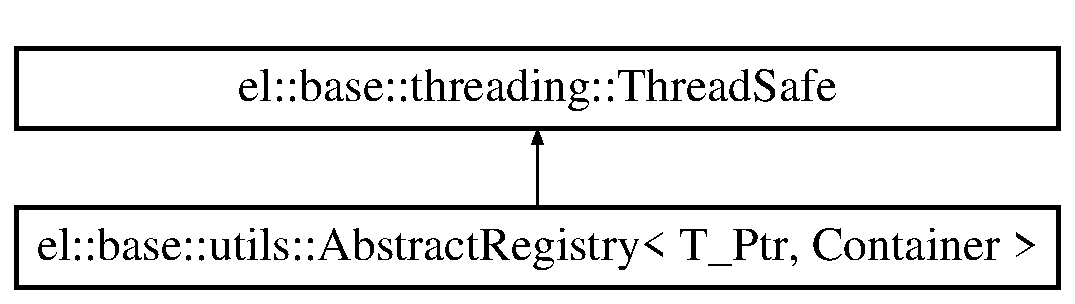
\includegraphics[height=2.000000cm]{classel_1_1base_1_1utils_1_1AbstractRegistry}
\end{center}
\end{figure}
\subsection*{Public Types}
\begin{DoxyCompactItemize}
\item 
\hypertarget{classel_1_1base_1_1utils_1_1AbstractRegistry_a58d0536c748633afd3f7c237b63a9a7c}{typedef Container\-::iterator {\bfseries iterator}}\label{classel_1_1base_1_1utils_1_1AbstractRegistry_a58d0536c748633afd3f7c237b63a9a7c}

\item 
\hypertarget{classel_1_1base_1_1utils_1_1AbstractRegistry_a3bbf19b112c067cb1a02a82b003cc7e2}{typedef Container\-::const\-\_\-iterator {\bfseries const\-\_\-iterator}}\label{classel_1_1base_1_1utils_1_1AbstractRegistry_a3bbf19b112c067cb1a02a82b003cc7e2}

\end{DoxyCompactItemize}
\subsection*{Public Member Functions}
\begin{DoxyCompactItemize}
\item 
\hypertarget{classel_1_1base_1_1utils_1_1AbstractRegistry_afe13c67ebd1ed1aa72845926894dffa2}{\hyperlink{classel_1_1base_1_1utils_1_1AbstractRegistry_afe13c67ebd1ed1aa72845926894dffa2}{Abstract\-Registry} (void)}\label{classel_1_1base_1_1utils_1_1AbstractRegistry_afe13c67ebd1ed1aa72845926894dffa2}

\begin{DoxyCompactList}\small\item\em Default constructor. \end{DoxyCompactList}\item 
\hypertarget{classel_1_1base_1_1utils_1_1AbstractRegistry_a9f468010439d491e90419f9334afcdba}{\hyperlink{classel_1_1base_1_1utils_1_1AbstractRegistry_a9f468010439d491e90419f9334afcdba}{Abstract\-Registry} (\hyperlink{classel_1_1base_1_1utils_1_1AbstractRegistry}{Abstract\-Registry} \&\&sr)}\label{classel_1_1base_1_1utils_1_1AbstractRegistry_a9f468010439d491e90419f9334afcdba}

\begin{DoxyCompactList}\small\item\em Move constructor that is useful for base classes. \end{DoxyCompactList}\item 
\hypertarget{classel_1_1base_1_1utils_1_1AbstractRegistry_ac3e648dc0caa8914f8604650f00bc94b}{bool {\bfseries operator==} (const \hyperlink{classel_1_1base_1_1utils_1_1AbstractRegistry}{Abstract\-Registry}$<$ T\-\_\-\-Ptr, Container $>$ \&other)}\label{classel_1_1base_1_1utils_1_1AbstractRegistry_ac3e648dc0caa8914f8604650f00bc94b}

\item 
\hypertarget{classel_1_1base_1_1utils_1_1AbstractRegistry_a35de8807521651c85acb26532a2623e1}{bool {\bfseries operator!=} (const \hyperlink{classel_1_1base_1_1utils_1_1AbstractRegistry}{Abstract\-Registry}$<$ T\-\_\-\-Ptr, Container $>$ \&other)}\label{classel_1_1base_1_1utils_1_1AbstractRegistry_a35de8807521651c85acb26532a2623e1}

\item 
\hypertarget{classel_1_1base_1_1utils_1_1AbstractRegistry_a5727a3cadeee6a2b10d8f46fb91956e7}{\hyperlink{classel_1_1base_1_1utils_1_1AbstractRegistry}{Abstract\-Registry} \& \hyperlink{classel_1_1base_1_1utils_1_1AbstractRegistry_a5727a3cadeee6a2b10d8f46fb91956e7}{operator=} (\hyperlink{classel_1_1base_1_1utils_1_1AbstractRegistry}{Abstract\-Registry} \&\&sr)}\label{classel_1_1base_1_1utils_1_1AbstractRegistry_a5727a3cadeee6a2b10d8f46fb91956e7}

\begin{DoxyCompactList}\small\item\em Assignment move operator. \end{DoxyCompactList}\item 
virtual iterator \hyperlink{classel_1_1base_1_1utils_1_1AbstractRegistry_a4ad971b1dddff996d327452d852e55b2}{begin} (void) E\-L\-P\-P\-\_\-\-F\-I\-N\-A\-L
\item 
virtual iterator \hyperlink{classel_1_1base_1_1utils_1_1AbstractRegistry_a67c40207c171f23ad50a71db819e84f9}{end} (void) E\-L\-P\-P\-\_\-\-F\-I\-N\-A\-L
\item 
virtual const\-\_\-iterator \hyperlink{classel_1_1base_1_1utils_1_1AbstractRegistry_a37f743184e808d7c0028e21e0d0898bb}{cbegin} (void) const E\-L\-P\-P\-\_\-\-F\-I\-N\-A\-L
\item 
virtual const\-\_\-iterator \hyperlink{classel_1_1base_1_1utils_1_1AbstractRegistry_ad3ee081b4b25c5d77f971f949bdb9158}{cend} (void) const E\-L\-P\-P\-\_\-\-F\-I\-N\-A\-L
\item 
virtual bool \hyperlink{classel_1_1base_1_1utils_1_1AbstractRegistry_a43ff6484b778c298416c482c07a4df3f}{empty} (void) const E\-L\-P\-P\-\_\-\-F\-I\-N\-A\-L
\item 
virtual std\-::size\-\_\-t \hyperlink{classel_1_1base_1_1utils_1_1AbstractRegistry_a58a7b8ea964bdf6008701dcfb6609ca5}{size} (void) const E\-L\-P\-P\-\_\-\-F\-I\-N\-A\-L
\item 
\hypertarget{classel_1_1base_1_1utils_1_1AbstractRegistry_a072859d3728a75f910c2898f62fd12da}{virtual Container \& \hyperlink{classel_1_1base_1_1utils_1_1AbstractRegistry_a072859d3728a75f910c2898f62fd12da}{list} (void) E\-L\-P\-P\-\_\-\-F\-I\-N\-A\-L}\label{classel_1_1base_1_1utils_1_1AbstractRegistry_a072859d3728a75f910c2898f62fd12da}

\begin{DoxyCompactList}\small\item\em Returns underlying container by reference. \end{DoxyCompactList}\item 
\hypertarget{classel_1_1base_1_1utils_1_1AbstractRegistry_a1c3da2af9177cbfae6f10b9e5dbe615c}{virtual const Container \& \hyperlink{classel_1_1base_1_1utils_1_1AbstractRegistry_a1c3da2af9177cbfae6f10b9e5dbe615c}{list} (void) const E\-L\-P\-P\-\_\-\-F\-I\-N\-A\-L}\label{classel_1_1base_1_1utils_1_1AbstractRegistry_a1c3da2af9177cbfae6f10b9e5dbe615c}

\begin{DoxyCompactList}\small\item\em Returns underlying container by constant reference. \end{DoxyCompactList}\item 
\hypertarget{classel_1_1base_1_1utils_1_1AbstractRegistry_a19223bc1fea48dbe6b47b4879aa4672f}{virtual void \hyperlink{classel_1_1base_1_1utils_1_1AbstractRegistry_a19223bc1fea48dbe6b47b4879aa4672f}{unregister\-All} (void)=0}\label{classel_1_1base_1_1utils_1_1AbstractRegistry_a19223bc1fea48dbe6b47b4879aa4672f}

\begin{DoxyCompactList}\small\item\em Unregisters all the pointers from current repository. \end{DoxyCompactList}\end{DoxyCompactItemize}
\subsection*{Protected Member Functions}
\begin{DoxyCompactItemize}
\item 
\hypertarget{classel_1_1base_1_1utils_1_1AbstractRegistry_aaf42dab7089a9b1198e2920983ca82bb}{virtual void {\bfseries deep\-Copy} (const \hyperlink{classel_1_1base_1_1utils_1_1AbstractRegistry}{Abstract\-Registry}$<$ T\-\_\-\-Ptr, Container $>$ \&)=0}\label{classel_1_1base_1_1utils_1_1AbstractRegistry_aaf42dab7089a9b1198e2920983ca82bb}

\item 
\hypertarget{classel_1_1base_1_1utils_1_1AbstractRegistry_a529677fb42e78d03c36cdea49f8877c9}{void {\bfseries reinit\-Deep\-Copy} (const \hyperlink{classel_1_1base_1_1utils_1_1AbstractRegistry}{Abstract\-Registry}$<$ T\-\_\-\-Ptr, Container $>$ \&sr)}\label{classel_1_1base_1_1utils_1_1AbstractRegistry_a529677fb42e78d03c36cdea49f8877c9}

\end{DoxyCompactItemize}


\subsection{Detailed Description}
\subsubsection*{template$<$typename T\-\_\-\-Ptr, typename Container$>$class el\-::base\-::utils\-::\-Abstract\-Registry$<$ T\-\_\-\-Ptr, Container $>$}

Abstract registry (aka repository) that provides basic interface for pointer repository specified by T\-\_\-\-Ptr type. 

Most of the functions are virtual final methods but anything implementing this abstract class should implement \hyperlink{classel_1_1base_1_1utils_1_1AbstractRegistry_a19223bc1fea48dbe6b47b4879aa4672f}{unregister\-All()} and deep\-Copy(const Abstract\-Registry$<$\-T\-\_\-\-Ptr, Container$>$\&) and write register\-New() method according to container and few more methods; get() to find element, unregister() to unregister single entry. Please note that this is thread-\/unsafe and should also implement thread-\/safety mechanisms in implementation. 

\subsection{Member Function Documentation}
\hypertarget{classel_1_1base_1_1utils_1_1AbstractRegistry_a4ad971b1dddff996d327452d852e55b2}{\index{el\-::base\-::utils\-::\-Abstract\-Registry@{el\-::base\-::utils\-::\-Abstract\-Registry}!begin@{begin}}
\index{begin@{begin}!el::base::utils::AbstractRegistry@{el\-::base\-::utils\-::\-Abstract\-Registry}}
\subsubsection[{begin}]{\setlength{\rightskip}{0pt plus 5cm}template$<$typename T\-\_\-\-Ptr, typename Container$>$ virtual iterator {\bf el\-::base\-::utils\-::\-Abstract\-Registry}$<$ T\-\_\-\-Ptr, Container $>$\-::begin (
\begin{DoxyParamCaption}
\item[{void}]{}
\end{DoxyParamCaption}
)\hspace{0.3cm}{\ttfamily [inline]}, {\ttfamily [virtual]}}}\label{classel_1_1base_1_1utils_1_1AbstractRegistry_a4ad971b1dddff996d327452d852e55b2}
\begin{DoxyReturn}{Returns}
Iterator pointer from start of repository 
\end{DoxyReturn}
\hypertarget{classel_1_1base_1_1utils_1_1AbstractRegistry_a37f743184e808d7c0028e21e0d0898bb}{\index{el\-::base\-::utils\-::\-Abstract\-Registry@{el\-::base\-::utils\-::\-Abstract\-Registry}!cbegin@{cbegin}}
\index{cbegin@{cbegin}!el::base::utils::AbstractRegistry@{el\-::base\-::utils\-::\-Abstract\-Registry}}
\subsubsection[{cbegin}]{\setlength{\rightskip}{0pt plus 5cm}template$<$typename T\-\_\-\-Ptr, typename Container$>$ virtual const\-\_\-iterator {\bf el\-::base\-::utils\-::\-Abstract\-Registry}$<$ T\-\_\-\-Ptr, Container $>$\-::cbegin (
\begin{DoxyParamCaption}
\item[{void}]{}
\end{DoxyParamCaption}
) const\hspace{0.3cm}{\ttfamily [inline]}, {\ttfamily [virtual]}}}\label{classel_1_1base_1_1utils_1_1AbstractRegistry_a37f743184e808d7c0028e21e0d0898bb}
\begin{DoxyReturn}{Returns}
Constant iterator pointer from start of repository 
\end{DoxyReturn}
\hypertarget{classel_1_1base_1_1utils_1_1AbstractRegistry_ad3ee081b4b25c5d77f971f949bdb9158}{\index{el\-::base\-::utils\-::\-Abstract\-Registry@{el\-::base\-::utils\-::\-Abstract\-Registry}!cend@{cend}}
\index{cend@{cend}!el::base::utils::AbstractRegistry@{el\-::base\-::utils\-::\-Abstract\-Registry}}
\subsubsection[{cend}]{\setlength{\rightskip}{0pt plus 5cm}template$<$typename T\-\_\-\-Ptr, typename Container$>$ virtual const\-\_\-iterator {\bf el\-::base\-::utils\-::\-Abstract\-Registry}$<$ T\-\_\-\-Ptr, Container $>$\-::cend (
\begin{DoxyParamCaption}
\item[{void}]{}
\end{DoxyParamCaption}
) const\hspace{0.3cm}{\ttfamily [inline]}, {\ttfamily [virtual]}}}\label{classel_1_1base_1_1utils_1_1AbstractRegistry_ad3ee081b4b25c5d77f971f949bdb9158}
\begin{DoxyReturn}{Returns}
End of repository 
\end{DoxyReturn}
\hypertarget{classel_1_1base_1_1utils_1_1AbstractRegistry_a43ff6484b778c298416c482c07a4df3f}{\index{el\-::base\-::utils\-::\-Abstract\-Registry@{el\-::base\-::utils\-::\-Abstract\-Registry}!empty@{empty}}
\index{empty@{empty}!el::base::utils::AbstractRegistry@{el\-::base\-::utils\-::\-Abstract\-Registry}}
\subsubsection[{empty}]{\setlength{\rightskip}{0pt plus 5cm}template$<$typename T\-\_\-\-Ptr, typename Container$>$ virtual bool {\bf el\-::base\-::utils\-::\-Abstract\-Registry}$<$ T\-\_\-\-Ptr, Container $>$\-::empty (
\begin{DoxyParamCaption}
\item[{void}]{}
\end{DoxyParamCaption}
) const\hspace{0.3cm}{\ttfamily [inline]}, {\ttfamily [virtual]}}}\label{classel_1_1base_1_1utils_1_1AbstractRegistry_a43ff6484b778c298416c482c07a4df3f}
\begin{DoxyReturn}{Returns}
Whether or not repository is empty 
\end{DoxyReturn}
\hypertarget{classel_1_1base_1_1utils_1_1AbstractRegistry_a67c40207c171f23ad50a71db819e84f9}{\index{el\-::base\-::utils\-::\-Abstract\-Registry@{el\-::base\-::utils\-::\-Abstract\-Registry}!end@{end}}
\index{end@{end}!el::base::utils::AbstractRegistry@{el\-::base\-::utils\-::\-Abstract\-Registry}}
\subsubsection[{end}]{\setlength{\rightskip}{0pt plus 5cm}template$<$typename T\-\_\-\-Ptr, typename Container$>$ virtual iterator {\bf el\-::base\-::utils\-::\-Abstract\-Registry}$<$ T\-\_\-\-Ptr, Container $>$\-::end (
\begin{DoxyParamCaption}
\item[{void}]{}
\end{DoxyParamCaption}
)\hspace{0.3cm}{\ttfamily [inline]}, {\ttfamily [virtual]}}}\label{classel_1_1base_1_1utils_1_1AbstractRegistry_a67c40207c171f23ad50a71db819e84f9}
\begin{DoxyReturn}{Returns}
Iterator pointer from end of repository 
\end{DoxyReturn}
\hypertarget{classel_1_1base_1_1utils_1_1AbstractRegistry_a58a7b8ea964bdf6008701dcfb6609ca5}{\index{el\-::base\-::utils\-::\-Abstract\-Registry@{el\-::base\-::utils\-::\-Abstract\-Registry}!size@{size}}
\index{size@{size}!el::base::utils::AbstractRegistry@{el\-::base\-::utils\-::\-Abstract\-Registry}}
\subsubsection[{size}]{\setlength{\rightskip}{0pt plus 5cm}template$<$typename T\-\_\-\-Ptr, typename Container$>$ virtual std\-::size\-\_\-t {\bf el\-::base\-::utils\-::\-Abstract\-Registry}$<$ T\-\_\-\-Ptr, Container $>$\-::size (
\begin{DoxyParamCaption}
\item[{void}]{}
\end{DoxyParamCaption}
) const\hspace{0.3cm}{\ttfamily [inline]}, {\ttfamily [virtual]}}}\label{classel_1_1base_1_1utils_1_1AbstractRegistry_a58a7b8ea964bdf6008701dcfb6609ca5}
\begin{DoxyReturn}{Returns}
Size of repository 
\end{DoxyReturn}


The documentation for this class was generated from the following file\-:\begin{DoxyCompactItemize}
\item 
include/sma/io/detail/logimpl.\-hpp\end{DoxyCompactItemize}

\hypertarget{structsma_1_1Action}{\section{sma\-:\-:Action Struct Reference}
\label{structsma_1_1Action}\index{sma\-::\-Action@{sma\-::\-Action}}
}
Inheritance diagram for sma\-:\-:Action\-:\begin{figure}[H]
\begin{center}
\leavevmode
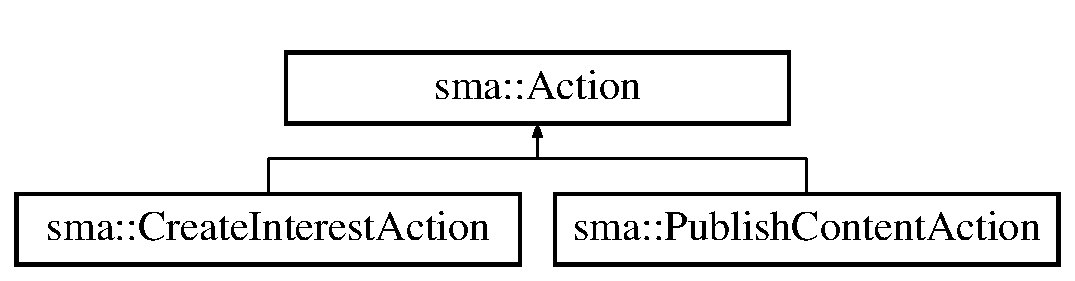
\includegraphics[height=2.000000cm]{structsma_1_1Action}
\end{center}
\end{figure}
\subsection*{Public Types}
\begin{DoxyCompactItemize}
\item 
\hypertarget{structsma_1_1Action_abcfa737ef02486538edcc5df649b0392}{using {\bfseries nanos} = std\-::chrono\-::nanoseconds}\label{structsma_1_1Action_abcfa737ef02486538edcc5df649b0392}

\item 
\hypertarget{structsma_1_1Action_a3f00650e4dc9cdcadfb31ffc02fbc5a5}{using {\bfseries delay\-\_\-unit} = nanos}\label{structsma_1_1Action_a3f00650e4dc9cdcadfb31ffc02fbc5a5}

\end{DoxyCompactItemize}
\subsection*{Public Member Functions}
\begin{DoxyCompactItemize}
\item 
\hypertarget{structsma_1_1Action_a7eaa3415defd12f4ab8720009499097e}{{\bfseries Action} (\hyperlink{classsma_1_1Ns3NodeContainer}{Ns3\-Node\-Container} \&context)}\label{structsma_1_1Action_a7eaa3415defd12f4ab8720009499097e}

\item 
\hypertarget{structsma_1_1Action_a5bb8f22a7e77cdf7c8cfd3fee7d90c09}{virtual void {\bfseries operator()} ()=0}\label{structsma_1_1Action_a5bb8f22a7e77cdf7c8cfd3fee7d90c09}

\item 
\hypertarget{structsma_1_1Action_a8cdbc5cbd2733992376eab1538cb2874}{nanos {\bfseries remaining\-\_\-delay\-\_\-ns} ()}\label{structsma_1_1Action_a8cdbc5cbd2733992376eab1538cb2874}

\end{DoxyCompactItemize}
\subsection*{Static Public Member Functions}
\begin{DoxyCompactItemize}
\item 
\hypertarget{structsma_1_1Action_a9fb0067a41679d83f6f60d16a4aa3fb6}{{\footnotesize template$<$typename Duration $>$ }\\static nanos {\bfseries delay\-\_\-to\-\_\-absolute} (Duration const \&delay)}\label{structsma_1_1Action_a9fb0067a41679d83f6f60d16a4aa3fb6}

\end{DoxyCompactItemize}
\subsection*{Public Attributes}
\begin{DoxyCompactItemize}
\item 
\hypertarget{structsma_1_1Action_a7af95774e1af5fa6618c60e108a6f9e4}{\hyperlink{classsma_1_1Ns3NodeContainer}{Ns3\-Node\-Container} $\ast$ {\bfseries context}}\label{structsma_1_1Action_a7af95774e1af5fa6618c60e108a6f9e4}

\item 
nanos \hyperlink{structsma_1_1Action_ae0e6be0e4548f1f27d4818e4d23ddbcf}{time}
\item 
\hypertarget{structsma_1_1Action_a3b6cf7ebcc195b0125f6da2ca6035233}{ns3\-::\-Event\-Id {\bfseries event\-\_\-id}}\label{structsma_1_1Action_a3b6cf7ebcc195b0125f6da2ca6035233}

\end{DoxyCompactItemize}


\subsection{Member Data Documentation}
\hypertarget{structsma_1_1Action_ae0e6be0e4548f1f27d4818e4d23ddbcf}{\index{sma\-::\-Action@{sma\-::\-Action}!time@{time}}
\index{time@{time}!sma::Action@{sma\-::\-Action}}
\subsubsection[{time}]{\setlength{\rightskip}{0pt plus 5cm}nanos sma\-::\-Action\-::time}}\label{structsma_1_1Action_ae0e6be0e4548f1f27d4818e4d23ddbcf}
Absolute time at which this action will execute. 

The documentation for this struct was generated from the following file\-:\begin{DoxyCompactItemize}
\item 
ns3/include/sma/ns3/action.\-hpp\end{DoxyCompactItemize}

\hypertarget{structsma_1_1Async}{\section{sma\-:\-:Async Struct Reference}
\label{structsma_1_1Async}\index{sma\-::\-Async@{sma\-::\-Async}}
}
\subsection*{Static Public Member Functions}
\begin{DoxyCompactItemize}
\item 
\hypertarget{structsma_1_1Async_a88e8ad75e75506162a0197cf51cebc4e}{static void {\bfseries purge} ()}\label{structsma_1_1Async_a88e8ad75e75506162a0197cf51cebc4e}

\item 
\hypertarget{structsma_1_1Async_a1200e37ea6b493a8019ac73d9072ef20}{static void {\bfseries schedule} (std\-::function$<$ void()$>$ f, std\-::chrono\-::nanoseconds delay)}\label{structsma_1_1Async_a1200e37ea6b493a8019ac73d9072ef20}

\end{DoxyCompactItemize}


The documentation for this struct was generated from the following files\-:\begin{DoxyCompactItemize}
\item 
include/sma/async.\-hpp\item 
ns3/src/async.\-cpp\end{DoxyCompactItemize}

\hypertarget{structsma_1_1AsyncTask}{\section{sma\-:\-:Async\-Task$<$ F, A $>$ Struct Template Reference}
\label{structsma_1_1AsyncTask}\index{sma\-::\-Async\-Task$<$ F, A $>$@{sma\-::\-Async\-Task$<$ F, A $>$}}
}
\subsection*{Public Types}
\begin{DoxyCompactItemize}
\item 
\hypertarget{structsma_1_1AsyncTask_aed4904d195c75e0b369cfde8e46580e4}{using {\bfseries result\-\_\-type} = typename std\-::result\-\_\-of$<$ F(A...)$>$\-::type}\label{structsma_1_1AsyncTask_aed4904d195c75e0b369cfde8e46580e4}

\end{DoxyCompactItemize}
\subsection*{Public Member Functions}
\begin{DoxyCompactItemize}
\item 
\hypertarget{structsma_1_1AsyncTask_ab4115ad8a8656927f5c0101ca156d285}{{\bfseries Async\-Task} (F \&\&f, A \&\&...args)}\label{structsma_1_1AsyncTask_ab4115ad8a8656927f5c0101ca156d285}

\item 
\hypertarget{structsma_1_1AsyncTask_a4dbf42e95a13f8e311083e6fb2dd0191}{{\bfseries Async\-Task} (\hyperlink{structsma_1_1AsyncTask}{Async\-Task} \&\&t)}\label{structsma_1_1AsyncTask_a4dbf42e95a13f8e311083e6fb2dd0191}

\item 
\hypertarget{structsma_1_1AsyncTask_a3dcd19e457ad82875ef15b1846574130}{\hyperlink{structsma_1_1AsyncTask}{Async\-Task} \& {\bfseries operator=} (\hyperlink{structsma_1_1AsyncTask}{Async\-Task} \&\&t)}\label{structsma_1_1AsyncTask_a3dcd19e457ad82875ef15b1846574130}

\item 
\hypertarget{structsma_1_1AsyncTask_a9d9902495f9b8b02911d83d81bef5a44}{{\footnotesize template$<$typename Delay $>$ }\\std\-::future$<$ result\-\_\-type $>$ {\bfseries do\-\_\-in} (Delay delay)}\label{structsma_1_1AsyncTask_a9d9902495f9b8b02911d83d81bef5a44}

\item 
\hypertarget{structsma_1_1AsyncTask_a01847bbf15f739c525dc014cf750d842}{std\-::future$<$ result\-\_\-type $>$ {\bfseries do\-\_\-now} ()}\label{structsma_1_1AsyncTask_a01847bbf15f739c525dc014cf750d842}

\item 
\hypertarget{structsma_1_1AsyncTask_a77b3df2fe421a69a8df41618dbe167d3}{{\footnotesize template$<$typename Delay $>$ }\\std\-::future$<$ typename \\*
\hyperlink{structsma_1_1AsyncTask}{Async\-Task}$<$ F, A...$>$\\*
\-::result\-\_\-type $>$ {\bfseries do\-\_\-in} (Delay delay)}\label{structsma_1_1AsyncTask_a77b3df2fe421a69a8df41618dbe167d3}

\end{DoxyCompactItemize}


The documentation for this struct was generated from the following file\-:\begin{DoxyCompactItemize}
\item 
include/sma/async.\-hpp\end{DoxyCompactItemize}

\hypertarget{structsma_1_1Beacon}{\section{sma\-:\-:Beacon Struct Reference}
\label{structsma_1_1Beacon}\index{sma\-::\-Beacon@{sma\-::\-Beacon}}
}
\subsection*{Public Types}
\begin{DoxyCompactItemize}
\item 
\hypertarget{structsma_1_1Beacon_a0741055c7878d65e7340f894b82f1a16}{using {\bfseries size\-\_\-type} = std\-::uint8\-\_\-t}\label{structsma_1_1Beacon_a0741055c7878d65e7340f894b82f1a16}

\item 
\hypertarget{structsma_1_1Beacon_a628b27b3ae761f374e32000410b5f390}{using {\bfseries body\-\_\-type} = \hyperlink{structsma_1_1Buffer}{Buffer}$<$ size\-\_\-type $>$}\label{structsma_1_1Beacon_a628b27b3ae761f374e32000410b5f390}

\end{DoxyCompactItemize}
\subsection*{Public Member Functions}
\begin{DoxyCompactItemize}
\item 
\hypertarget{structsma_1_1Beacon_a987e5a3aafe40aaccdc1b9b08df7efed}{{\bfseries Beacon} (\hyperlink{structsma_1_1Buffer}{body\-\_\-type} body)}\label{structsma_1_1Beacon_a987e5a3aafe40aaccdc1b9b08df7efed}

\item 
\hypertarget{structsma_1_1Beacon_a7c2f34666a86f7980ca9d433a7b10831}{{\bfseries Beacon} (\hyperlink{structsma_1_1Beacon}{Beacon} \&\&)=default}\label{structsma_1_1Beacon_a7c2f34666a86f7980ca9d433a7b10831}

\item 
\hypertarget{structsma_1_1Beacon_ad3b2e73ab9333644c75725065bd79aa9}{{\bfseries Beacon} (\hyperlink{structsma_1_1Beacon}{Beacon} const \&)=default}\label{structsma_1_1Beacon_ad3b2e73ab9333644c75725065bd79aa9}

\item 
\hypertarget{structsma_1_1Beacon_a74dc09ac64bccacaa975274b956326db}{\hyperlink{structsma_1_1Beacon}{Beacon} \& {\bfseries operator=} (\hyperlink{structsma_1_1Beacon}{Beacon} \&\&)=default}\label{structsma_1_1Beacon_a74dc09ac64bccacaa975274b956326db}

\item 
\hypertarget{structsma_1_1Beacon_abba9dcdeffb2c0c24441d9a32aa2d51a}{\hyperlink{structsma_1_1Beacon}{Beacon} \& {\bfseries operator=} (\hyperlink{structsma_1_1Beacon}{Beacon} const \&)=default}\label{structsma_1_1Beacon_abba9dcdeffb2c0c24441d9a32aa2d51a}

\end{DoxyCompactItemize}
\subsection*{Public Attributes}
\begin{DoxyCompactItemize}
\item 
\hypertarget{structsma_1_1Beacon_a1dfddd2a8cd3ab94e501d0861b4d0157}{\hyperlink{structsma_1_1Buffer}{body\-\_\-type} {\bfseries body}}\label{structsma_1_1Beacon_a1dfddd2a8cd3ab94e501d0861b4d0157}

\end{DoxyCompactItemize}


The documentation for this struct was generated from the following file\-:\begin{DoxyCompactItemize}
\item 
include/sma/beacon.\-hpp\end{DoxyCompactItemize}

\hypertarget{classsma_1_1BinaryInput}{\section{sma\-:\-:Binary\-Input Class Reference}
\label{classsma_1_1BinaryInput}\index{sma\-::\-Binary\-Input@{sma\-::\-Binary\-Input}}
}
\subsection*{Public Member Functions}
\begin{DoxyCompactItemize}
\item 
\hypertarget{classsma_1_1BinaryInput_a03dae935b9d83e882da5e77ecfd8ebc9}{{\bfseries Binary\-Input} (std\-::istream \&is)}\label{classsma_1_1BinaryInput_a03dae935b9d83e882da5e77ecfd8ebc9}

\item 
\hypertarget{classsma_1_1BinaryInput_a1ccd9d0564d6e777544fee24bd7a99ab}{{\bfseries Binary\-Input} (\hyperlink{classsma_1_1BinaryInput}{Binary\-Input} const \&r)}\label{classsma_1_1BinaryInput_a1ccd9d0564d6e777544fee24bd7a99ab}

\item 
\hypertarget{classsma_1_1BinaryInput_a94e0016b49e429ec44b3e51f81d5a952}{\hyperlink{classsma_1_1BinaryInput}{Binary\-Input} \& {\bfseries operator=} (\hyperlink{classsma_1_1BinaryInput}{Binary\-Input} const \&r)}\label{classsma_1_1BinaryInput_a94e0016b49e429ec44b3e51f81d5a952}

\item 
\hypertarget{classsma_1_1BinaryInput_a33bb4e021d58a7e9615cdb8ebda5b4a2}{void $\ast$ {\bfseries read} (void $\ast$dst, std\-::size\-\_\-t size)}\label{classsma_1_1BinaryInput_a33bb4e021d58a7e9615cdb8ebda5b4a2}

\item 
\hypertarget{classsma_1_1BinaryInput_a605183bc9ff0506c287780a071319042}{{\footnotesize template$<$typename T $>$ }\\T {\bfseries get} ()}\label{classsma_1_1BinaryInput_a605183bc9ff0506c287780a071319042}

\item 
\hypertarget{classsma_1_1BinaryInput_a0c996cb47ed23163130c7ec2e55de5d1}{{\footnotesize template$<$typename T $>$ }\\\hyperlink{classsma_1_1BinaryInput}{Binary\-Input} {\bfseries operator$>$$>$} (T \&t)}\label{classsma_1_1BinaryInput_a0c996cb47ed23163130c7ec2e55de5d1}

\item 
\hypertarget{classsma_1_1BinaryInput_a573b369e69b08aebc193d85235645698}{{\footnotesize template$<$$>$ }\\float {\bfseries get} ()}\label{classsma_1_1BinaryInput_a573b369e69b08aebc193d85235645698}

\item 
\hypertarget{classsma_1_1BinaryInput_ab23a06827e2f9a260d531e1c0cd65b1a}{{\footnotesize template$<$$>$ }\\double {\bfseries get} ()}\label{classsma_1_1BinaryInput_ab23a06827e2f9a260d531e1c0cd65b1a}

\item 
\hypertarget{classsma_1_1BinaryInput_adece6dab3901b62aa6326138ac089d53}{{\footnotesize template$<$$>$ }\\std\-::string {\bfseries get} ()}\label{classsma_1_1BinaryInput_adece6dab3901b62aa6326138ac089d53}

\item 
\hypertarget{classsma_1_1BinaryInput_a573b369e69b08aebc193d85235645698}{{\footnotesize template$<$$>$ }\\float {\bfseries get} ()}\label{classsma_1_1BinaryInput_a573b369e69b08aebc193d85235645698}

\item 
\hypertarget{classsma_1_1BinaryInput_ab23a06827e2f9a260d531e1c0cd65b1a}{{\footnotesize template$<$$>$ }\\double {\bfseries get} ()}\label{classsma_1_1BinaryInput_ab23a06827e2f9a260d531e1c0cd65b1a}

\item 
\hypertarget{classsma_1_1BinaryInput_a766f69fbb2fe7cd4cc38c7219b1364e7}{{\footnotesize template$<$$>$ }\\std\-::uint8\-\_\-t {\bfseries get} ()}\label{classsma_1_1BinaryInput_a766f69fbb2fe7cd4cc38c7219b1364e7}

\item 
\hypertarget{classsma_1_1BinaryInput_ae2b8d53a92144a1ca3bd20e8b215b365}{{\footnotesize template$<$$>$ }\\std\-::uint16\-\_\-t {\bfseries get} ()}\label{classsma_1_1BinaryInput_ae2b8d53a92144a1ca3bd20e8b215b365}

\item 
\hypertarget{classsma_1_1BinaryInput_a19453b49aa0c78c7918af563062b37d7}{{\footnotesize template$<$$>$ }\\std\-::uint32\-\_\-t {\bfseries get} ()}\label{classsma_1_1BinaryInput_a19453b49aa0c78c7918af563062b37d7}

\item 
\hypertarget{classsma_1_1BinaryInput_aaf7e9d4151f38b813c295b2dd3d30bb9}{{\footnotesize template$<$$>$ }\\std\-::uint64\-\_\-t {\bfseries get} ()}\label{classsma_1_1BinaryInput_aaf7e9d4151f38b813c295b2dd3d30bb9}

\item 
\hypertarget{classsma_1_1BinaryInput_a8d14189773b657f8b95fe378aaa554fb}{{\footnotesize template$<$$>$ }\\std\-::int8\-\_\-t {\bfseries get} ()}\label{classsma_1_1BinaryInput_a8d14189773b657f8b95fe378aaa554fb}

\item 
\hypertarget{classsma_1_1BinaryInput_a99a6a795daf8bc512298187218c9a0b3}{{\footnotesize template$<$$>$ }\\std\-::int16\-\_\-t {\bfseries get} ()}\label{classsma_1_1BinaryInput_a99a6a795daf8bc512298187218c9a0b3}

\item 
\hypertarget{classsma_1_1BinaryInput_ad23c73d2c2113f4beb8e48c58f896293}{{\footnotesize template$<$$>$ }\\std\-::int32\-\_\-t {\bfseries get} ()}\label{classsma_1_1BinaryInput_ad23c73d2c2113f4beb8e48c58f896293}

\item 
\hypertarget{classsma_1_1BinaryInput_ace4718985e20551c8d530b4cb346c371}{{\footnotesize template$<$$>$ }\\std\-::int64\-\_\-t {\bfseries get} ()}\label{classsma_1_1BinaryInput_ace4718985e20551c8d530b4cb346c371}

\end{DoxyCompactItemize}


The documentation for this class was generated from the following files\-:\begin{DoxyCompactItemize}
\item 
include/sma/util/binaryinput.\-hpp\item 
src/util/binaryinput.\-cpp\end{DoxyCompactItemize}

\hypertarget{classsma_1_1BinaryOutput}{\section{sma\-:\-:Binary\-Output Class Reference}
\label{classsma_1_1BinaryOutput}\index{sma\-::\-Binary\-Output@{sma\-::\-Binary\-Output}}
}
\subsection*{Public Member Functions}
\begin{DoxyCompactItemize}
\item 
\hypertarget{classsma_1_1BinaryOutput_a0e7daf442b1f76ca0d919b01555f4abd}{{\bfseries Binary\-Output} (std\-::ostream \&os)}\label{classsma_1_1BinaryOutput_a0e7daf442b1f76ca0d919b01555f4abd}

\item 
\hypertarget{classsma_1_1BinaryOutput_a35fc0b2957c844399c3352c18d99fa70}{{\bfseries Binary\-Output} (\hyperlink{classsma_1_1BinaryOutput}{Binary\-Output} const \&r)}\label{classsma_1_1BinaryOutput_a35fc0b2957c844399c3352c18d99fa70}

\item 
\hypertarget{classsma_1_1BinaryOutput_a41fdb48541cdd9ee3e15ef8a8641c68e}{\hyperlink{classsma_1_1BinaryOutput}{Binary\-Output} \& {\bfseries operator=} (\hyperlink{classsma_1_1BinaryOutput}{Binary\-Output} const \&r)}\label{classsma_1_1BinaryOutput_a41fdb48541cdd9ee3e15ef8a8641c68e}

\item 
\hypertarget{classsma_1_1BinaryOutput_a1e51af2a691dba26e8d72facd1831c97}{\hyperlink{classsma_1_1BinaryOutput}{Binary\-Output} \& {\bfseries write} (void const $\ast$src, std\-::size\-\_\-t size)}\label{classsma_1_1BinaryOutput_a1e51af2a691dba26e8d72facd1831c97}

\item 
\hypertarget{classsma_1_1BinaryOutput_a98e9262d27c0b53d975e1b3708102073}{{\footnotesize template$<$typename T $>$ }\\\hyperlink{classsma_1_1BinaryOutput}{Binary\-Output} \& {\bfseries operator$<$$<$} (T const \&t)}\label{classsma_1_1BinaryOutput_a98e9262d27c0b53d975e1b3708102073}

\item 
\hypertarget{classsma_1_1BinaryOutput_a9b8b2919814081b98cc76beb5eeeb979}{{\footnotesize template$<$typename T $>$ }\\\hyperlink{classsma_1_1BinaryOutput}{Binary\-Output} \& {\bfseries operator$<$$<$} (std\-::vector$<$ T $>$ const \&v)}\label{classsma_1_1BinaryOutput_a9b8b2919814081b98cc76beb5eeeb979}

\item 
\hypertarget{classsma_1_1BinaryOutput_a8fbc2685044c755d5cbfbe889c77ecb4}{\hyperlink{classsma_1_1BinaryOutput}{Binary\-Output} \& {\bfseries operator$<$$<$} (std\-::string const \&t)}\label{classsma_1_1BinaryOutput_a8fbc2685044c755d5cbfbe889c77ecb4}

\item 
\hypertarget{classsma_1_1BinaryOutput_a68096960fc038164a7a063f85666eece}{\hyperlink{classsma_1_1BinaryOutput}{Binary\-Output} \& {\bfseries operator$<$$<$} (float const \&t)}\label{classsma_1_1BinaryOutput_a68096960fc038164a7a063f85666eece}

\item 
\hypertarget{classsma_1_1BinaryOutput_a06580481ee3c878dfbdaef3ca353ec60}{\hyperlink{classsma_1_1BinaryOutput}{Binary\-Output} \& {\bfseries operator$<$$<$} (double const \&t)}\label{classsma_1_1BinaryOutput_a06580481ee3c878dfbdaef3ca353ec60}

\item 
\hypertarget{classsma_1_1BinaryOutput_acfb30f63ded5970e309cfacd4823db2d}{\hyperlink{classsma_1_1BinaryOutput}{Binary\-Output} \& {\bfseries operator$<$$<$} (std\-::uint8\-\_\-t const \&t)}\label{classsma_1_1BinaryOutput_acfb30f63ded5970e309cfacd4823db2d}

\item 
\hypertarget{classsma_1_1BinaryOutput_a2f6f4aeaf81fb61637489fc7b8cc2e2d}{\hyperlink{classsma_1_1BinaryOutput}{Binary\-Output} \& {\bfseries operator$<$$<$} (std\-::uint16\-\_\-t const \&t)}\label{classsma_1_1BinaryOutput_a2f6f4aeaf81fb61637489fc7b8cc2e2d}

\item 
\hypertarget{classsma_1_1BinaryOutput_a40120522ba1b3fedc36aa213775d3dea}{\hyperlink{classsma_1_1BinaryOutput}{Binary\-Output} \& {\bfseries operator$<$$<$} (std\-::uint32\-\_\-t const \&t)}\label{classsma_1_1BinaryOutput_a40120522ba1b3fedc36aa213775d3dea}

\item 
\hypertarget{classsma_1_1BinaryOutput_ae1197d74aebcf767f1d81fa228ac8171}{\hyperlink{classsma_1_1BinaryOutput}{Binary\-Output} \& {\bfseries operator$<$$<$} (std\-::uint64\-\_\-t const \&t)}\label{classsma_1_1BinaryOutput_ae1197d74aebcf767f1d81fa228ac8171}

\item 
\hypertarget{classsma_1_1BinaryOutput_aecbcfb7860b286a009930816d04011e6}{\hyperlink{classsma_1_1BinaryOutput}{Binary\-Output} \& {\bfseries operator$<$$<$} (std\-::int8\-\_\-t const \&t)}\label{classsma_1_1BinaryOutput_aecbcfb7860b286a009930816d04011e6}

\item 
\hypertarget{classsma_1_1BinaryOutput_aeca8e6ebc97eb10a939b2e07e13bc635}{\hyperlink{classsma_1_1BinaryOutput}{Binary\-Output} \& {\bfseries operator$<$$<$} (std\-::int16\-\_\-t const \&t)}\label{classsma_1_1BinaryOutput_aeca8e6ebc97eb10a939b2e07e13bc635}

\item 
\hypertarget{classsma_1_1BinaryOutput_a15402d755d1fefa3ed45082fb8eb083b}{\hyperlink{classsma_1_1BinaryOutput}{Binary\-Output} \& {\bfseries operator$<$$<$} (std\-::int32\-\_\-t const \&t)}\label{classsma_1_1BinaryOutput_a15402d755d1fefa3ed45082fb8eb083b}

\item 
\hypertarget{classsma_1_1BinaryOutput_a50c528384783c433e2f04c6337278972}{\hyperlink{classsma_1_1BinaryOutput}{Binary\-Output} \& {\bfseries operator$<$$<$} (std\-::int64\-\_\-t const \&t)}\label{classsma_1_1BinaryOutput_a50c528384783c433e2f04c6337278972}

\end{DoxyCompactItemize}


The documentation for this class was generated from the following files\-:\begin{DoxyCompactItemize}
\item 
include/sma/util/binaryoutput.\-hpp\item 
src/util/binaryoutput.\-cpp\end{DoxyCompactItemize}

\hypertarget{classsma_1_1bsd__socket}{\section{sma\-:\-:bsd\-\_\-socket Class Reference}
\label{classsma_1_1bsd__socket}\index{sma\-::bsd\-\_\-socket@{sma\-::bsd\-\_\-socket}}
}
Inheritance diagram for sma\-:\-:bsd\-\_\-socket\-:\begin{figure}[H]
\begin{center}
\leavevmode
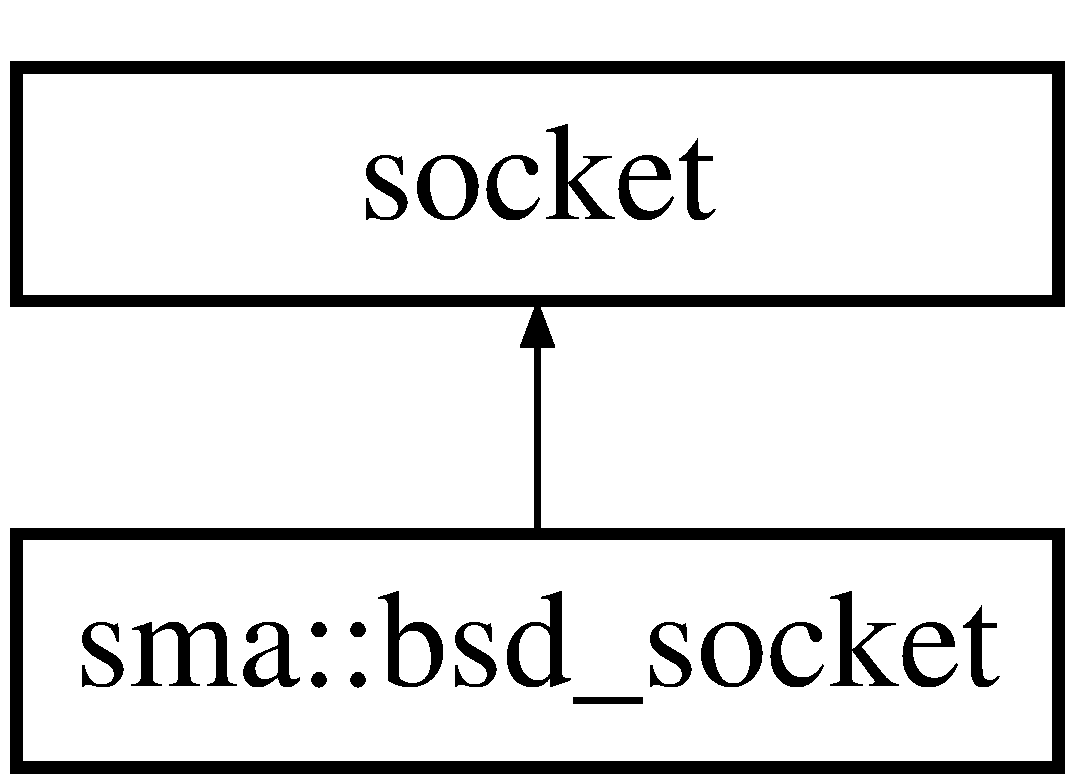
\includegraphics[height=2.000000cm]{classsma_1_1bsd__socket}
\end{center}
\end{figure}
\subsection*{Public Member Functions}
\begin{DoxyCompactItemize}
\item 
\hypertarget{classsma_1_1bsd__socket_a23f9938b524e14b5f14b8d2a9ba09038}{{\bfseries bsd\-\_\-socket} (protocol proto)}\label{classsma_1_1bsd__socket_a23f9938b524e14b5f14b8d2a9ba09038}

\item 
\hypertarget{classsma_1_1bsd__socket_afd5770cd9a7a4245575516ce8bb18a98}{void {\bfseries bind} (const socket\-\_\-addr \&address) override}\label{classsma_1_1bsd__socket_afd5770cd9a7a4245575516ce8bb18a98}

\item 
\hypertarget{classsma_1_1bsd__socket_a5113af941c9ba60391653542bc9bb69f}{void {\bfseries close} () override}\label{classsma_1_1bsd__socket_a5113af941c9ba60391653542bc9bb69f}

\item 
\hypertarget{classsma_1_1bsd__socket_abfd12d2ac34cd0aed4c5e33b76d3f651}{std\-::size\-\_\-t {\bfseries recv} (std\-::uint8\-\_\-t $\ast$dst, std\-::size\-\_\-t len) override}\label{classsma_1_1bsd__socket_abfd12d2ac34cd0aed4c5e33b76d3f651}

\item 
\hypertarget{classsma_1_1bsd__socket_a41c609b6761cc57f539e4449e5e601c6}{int {\bfseries send} (const std\-::uint8\-\_\-t $\ast$src, std\-::size\-\_\-t len, const socket\-\_\-addr \&recipient) override}\label{classsma_1_1bsd__socket_a41c609b6761cc57f539e4449e5e601c6}

\item 
\hypertarget{classsma_1_1bsd__socket_a0bdaeca951937be487bda6adaa5afc6a}{socket\-\_\-type {\bfseries native\-\_\-socket} () const noexcept}\label{classsma_1_1bsd__socket_a0bdaeca951937be487bda6adaa5afc6a}

\item 
\hypertarget{classsma_1_1bsd__socket_aa1848cfaed96e5a30e759990a7217b5d}{void {\bfseries blocking} (bool block)}\label{classsma_1_1bsd__socket_aa1848cfaed96e5a30e759990a7217b5d}

\item 
\hypertarget{classsma_1_1bsd__socket_ad21c78f0957ca922d67b0346aafddde4}{bool {\bfseries blocking} () const noexcept}\label{classsma_1_1bsd__socket_ad21c78f0957ca922d67b0346aafddde4}

\end{DoxyCompactItemize}


The documentation for this class was generated from the following files\-:\begin{DoxyCompactItemize}
\item 
android/core/include/sma/android/bsd\-\_\-socket.\-hpp\item 
android/core/src/net/inet/bsd\-\_\-socket.\-cc\item 
android/core/src/net/inet/bsd\-\_\-socket.\-cpp\end{DoxyCompactItemize}

\hypertarget{structsma_1_1Buffer}{\section{sma\-:\-:Buffer$<$ Size\-T $>$ Struct Template Reference}
\label{structsma_1_1Buffer}\index{sma\-::\-Buffer$<$ Size\-T $>$@{sma\-::\-Buffer$<$ Size\-T $>$}}
}
\subsection*{Public Member Functions}
\begin{DoxyCompactItemize}
\item 
\hypertarget{structsma_1_1Buffer_af75359b4a2a5b623c49a8eef50b72a1c}{{\bfseries Buffer} (std\-::size\-\_\-t size)}\label{structsma_1_1Buffer_af75359b4a2a5b623c49a8eef50b72a1c}

\item 
\hypertarget{structsma_1_1Buffer_a903f2dffc014914f612413b44365abfc}{{\bfseries Buffer} (std\-::uint8\-\_\-t const $\ast$data, std\-::size\-\_\-t size)}\label{structsma_1_1Buffer_a903f2dffc014914f612413b44365abfc}

\item 
\hypertarget{structsma_1_1Buffer_a410c9d6e0cee0465555f83a98b71a4cc}{{\bfseries Buffer} (\hyperlink{structsma_1_1Buffer}{Buffer} \&\&r)}\label{structsma_1_1Buffer_a410c9d6e0cee0465555f83a98b71a4cc}

\item 
\hypertarget{structsma_1_1Buffer_a915a33d5bb6396c0126dd3ec0e0f52ab}{{\bfseries Buffer} (\hyperlink{structsma_1_1Buffer}{Buffer} const \&r)}\label{structsma_1_1Buffer_a915a33d5bb6396c0126dd3ec0e0f52ab}

\item 
\hypertarget{structsma_1_1Buffer_aa6728160064fe204e8bb72fd512c514a}{\hyperlink{structsma_1_1Buffer}{Buffer} \& {\bfseries operator=} (\hyperlink{structsma_1_1Buffer}{Buffer} \&\&r)}\label{structsma_1_1Buffer_aa6728160064fe204e8bb72fd512c514a}

\item 
\hypertarget{structsma_1_1Buffer_ad00607f52dd911003503cd3b5e240958}{\hyperlink{structsma_1_1Buffer}{Buffer} \& {\bfseries operator=} (\hyperlink{structsma_1_1Buffer}{Buffer} const \&r)}\label{structsma_1_1Buffer_ad00607f52dd911003503cd3b5e240958}

\item 
\hypertarget{structsma_1_1Buffer_aae691e017440ca0902ea13896eb62140}{{\bfseries D\-E\-S\-E\-R\-I\-A\-L\-I\-Z\-I\-N\-G\-\_\-\-C\-T\-O\-R} (\hyperlink{structsma_1_1Buffer}{Buffer})}\label{structsma_1_1Buffer_aae691e017440ca0902ea13896eb62140}

\item 
\hypertarget{structsma_1_1Buffer_a884bdc40749615b1e4e12a1dfd1d0139}{{\bfseries S\-E\-R\-I\-A\-L\-I\-Z\-E\-R} ()}\label{structsma_1_1Buffer_a884bdc40749615b1e4e12a1dfd1d0139}

\item 
\hypertarget{structsma_1_1Buffer_acbbcb6b9e4edcca7d73f9faad16be4f4}{std\-::size\-\_\-t {\bfseries size} () const }\label{structsma_1_1Buffer_acbbcb6b9e4edcca7d73f9faad16be4f4}

\item 
\hypertarget{structsma_1_1Buffer_a05863812cbf141b22709ef2f39e30e40}{std\-::uint8\-\_\-t const $\ast$ {\bfseries cdata} () const }\label{structsma_1_1Buffer_a05863812cbf141b22709ef2f39e30e40}

\end{DoxyCompactItemize}


The documentation for this struct was generated from the following file\-:\begin{DoxyCompactItemize}
\item 
include/sma/util/buffer.\-hpp\end{DoxyCompactItemize}

\hypertarget{classsma_1_1BufferDest}{\section{sma\-:\-:Buffer\-Dest Class Reference}
\label{classsma_1_1BufferDest}\index{sma\-::\-Buffer\-Dest@{sma\-::\-Buffer\-Dest}}
}
\subsection*{Public Member Functions}
\begin{DoxyCompactItemize}
\item 
\hypertarget{classsma_1_1BufferDest_a0069ae2c6751ed8db3c275bcf625c0c2}{{\bfseries Buffer\-Dest} (std\-::size\-\_\-t size)}\label{classsma_1_1BufferDest_a0069ae2c6751ed8db3c275bcf625c0c2}

\item 
\hypertarget{classsma_1_1BufferDest_a41d3943720ab0e4233bb4747f46cfce7}{{\bfseries Buffer\-Dest} (char $\ast$dst, std\-::size\-\_\-t size)}\label{classsma_1_1BufferDest_a41d3943720ab0e4233bb4747f46cfce7}

\item 
\hypertarget{classsma_1_1BufferDest_acd931cafb3dd522826833e117db1086e}{{\bfseries Buffer\-Dest} (std\-::uint8\-\_\-t $\ast$dst, std\-::size\-\_\-t size)}\label{classsma_1_1BufferDest_acd931cafb3dd522826833e117db1086e}

\item 
\hypertarget{classsma_1_1BufferDest_a9d4ba8e11e57a90ea8bbcdb083c6f4d7}{{\footnotesize template$<$typename Formatter $>$ }\\Formatter {\bfseries format} ()}\label{classsma_1_1BufferDest_a9d4ba8e11e57a90ea8bbcdb083c6f4d7}

\item 
\hypertarget{classsma_1_1BufferDest_a99ee3b1da310fb5776aabef9f9b3439f}{std\-::size\-\_\-t {\bfseries size} ()}\label{classsma_1_1BufferDest_a99ee3b1da310fb5776aabef9f9b3439f}

\item 
\hypertarget{classsma_1_1BufferDest_ab1b010f817d8df6f3b3eecc69b36b9e5}{void {\bfseries rewind} ()}\label{classsma_1_1BufferDest_ab1b010f817d8df6f3b3eecc69b36b9e5}

\end{DoxyCompactItemize}


The documentation for this class was generated from the following files\-:\begin{DoxyCompactItemize}
\item 
include/sma/util/bufferdest.\-hpp\item 
src/util/bufferdest.\-cpp\end{DoxyCompactItemize}

\hypertarget{classsma_1_1BufferSource}{\section{sma\-:\-:Buffer\-Source Class Reference}
\label{classsma_1_1BufferSource}\index{sma\-::\-Buffer\-Source@{sma\-::\-Buffer\-Source}}
}
\subsection*{Public Member Functions}
\begin{DoxyCompactItemize}
\item 
\hypertarget{classsma_1_1BufferSource_a569bd9f1682d325d25fb8a595ed6d4f3}{{\bfseries Buffer\-Source} (char const $\ast$src, std\-::size\-\_\-t size)}\label{classsma_1_1BufferSource_a569bd9f1682d325d25fb8a595ed6d4f3}

\item 
\hypertarget{classsma_1_1BufferSource_afb8306209ad2990a8edc352bf1122de5}{{\bfseries Buffer\-Source} (std\-::uint8\-\_\-t const $\ast$src, std\-::size\-\_\-t size)}\label{classsma_1_1BufferSource_afb8306209ad2990a8edc352bf1122de5}

\item 
\hypertarget{classsma_1_1BufferSource_aec1d4d3784327463959bf8cfbe72089a}{void {\bfseries rewind} ()}\label{classsma_1_1BufferSource_aec1d4d3784327463959bf8cfbe72089a}

\item 
\hypertarget{classsma_1_1BufferSource_a14d5bc5fb45b103366f232d18b8cc67d}{{\footnotesize template$<$typename Formatter $>$ }\\\hyperlink{classsma_1_1Reader}{Reader}$<$ Formatter $>$ {\bfseries format} ()}\label{classsma_1_1BufferSource_a14d5bc5fb45b103366f232d18b8cc67d}

\end{DoxyCompactItemize}


The documentation for this class was generated from the following files\-:\begin{DoxyCompactItemize}
\item 
include/sma/util/buffersource.\-hpp\item 
src/util/buffersource.\-cpp\end{DoxyCompactItemize}

\hypertarget{classsma_1_1Bytes}{\section{sma\-:\-:Bytes Class Reference}
\label{classsma_1_1Bytes}\index{sma\-::\-Bytes@{sma\-::\-Bytes}}
}
\subsection*{Static Public Member Functions}
\begin{DoxyCompactItemize}
\item 
\hypertarget{classsma_1_1Bytes_a841e80738b98c0dbc86af2494bbc70d8}{static size\-\_\-t {\bfseries put} (uint8\-\_\-t $\ast$dst, const uint8\-\_\-t $\ast$src, size\-\_\-t len)}\label{classsma_1_1Bytes_a841e80738b98c0dbc86af2494bbc70d8}

\item 
\hypertarget{classsma_1_1Bytes_ae5b6a19877e5fc784a3da03cff3a8640}{static size\-\_\-t {\bfseries put} (uint8\-\_\-t $\ast$dst, const uint8\-\_\-t b)}\label{classsma_1_1Bytes_ae5b6a19877e5fc784a3da03cff3a8640}

\item 
\hypertarget{classsma_1_1Bytes_a21dac037bafc4351e3bfe1eb7c8bea7f}{static size\-\_\-t {\bfseries put} (uint8\-\_\-t $\ast$dst, const uint16\-\_\-t s)}\label{classsma_1_1Bytes_a21dac037bafc4351e3bfe1eb7c8bea7f}

\item 
\hypertarget{classsma_1_1Bytes_a834cafc63eb0a396d07c11cca4c5dc29}{static size\-\_\-t {\bfseries put} (uint8\-\_\-t $\ast$dst, const uint32\-\_\-t i)}\label{classsma_1_1Bytes_a834cafc63eb0a396d07c11cca4c5dc29}

\item 
\hypertarget{classsma_1_1Bytes_a0191a7143826b51481889e1d49ae4f20}{static size\-\_\-t {\bfseries get} (const uint8\-\_\-t $\ast$src, uint8\-\_\-t \&b)}\label{classsma_1_1Bytes_a0191a7143826b51481889e1d49ae4f20}

\item 
\hypertarget{classsma_1_1Bytes_ac9b59a33bd36fb405fb593e8ad51b3d6}{static size\-\_\-t {\bfseries get} (const uint8\-\_\-t $\ast$src, uint16\-\_\-t \&s)}\label{classsma_1_1Bytes_ac9b59a33bd36fb405fb593e8ad51b3d6}

\item 
\hypertarget{classsma_1_1Bytes_a5953d9e30c8f9a78ef8521ce7f5f51bc}{static size\-\_\-t {\bfseries get} (const uint8\-\_\-t $\ast$src, uint32\-\_\-t \&i)}\label{classsma_1_1Bytes_a5953d9e30c8f9a78ef8521ce7f5f51bc}

\end{DoxyCompactItemize}


The documentation for this class was generated from the following file\-:\begin{DoxyCompactItemize}
\item 
include/sma/util/bytes.\-hpp\end{DoxyCompactItemize}

\hypertarget{classel_1_1Callback}{\section{el\-:\-:Callback$<$ T $>$ Class Template Reference}
\label{classel_1_1Callback}\index{el\-::\-Callback$<$ T $>$@{el\-::\-Callback$<$ T $>$}}
}
Inheritance diagram for el\-:\-:Callback$<$ T $>$\-:\begin{figure}[H]
\begin{center}
\leavevmode
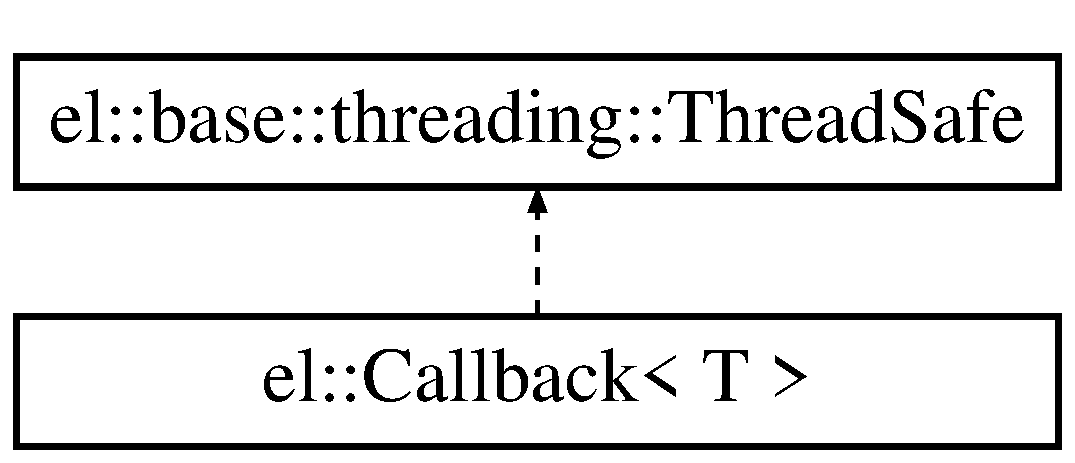
\includegraphics[height=2.000000cm]{classel_1_1Callback}
\end{center}
\end{figure}
\subsection*{Public Member Functions}
\begin{DoxyCompactItemize}
\item 
\hypertarget{classel_1_1Callback_a1e3089fd19a11965e7b98bd423116bbd}{bool {\bfseries enabled} (void) const }\label{classel_1_1Callback_a1e3089fd19a11965e7b98bd423116bbd}

\item 
\hypertarget{classel_1_1Callback_a05e68cb0b5ea4423913fa2ec4ea306b4}{void {\bfseries set\-Enabled} (bool enabled)}\label{classel_1_1Callback_a05e68cb0b5ea4423913fa2ec4ea306b4}

\end{DoxyCompactItemize}
\subsection*{Protected Member Functions}
\begin{DoxyCompactItemize}
\item 
\hypertarget{classel_1_1Callback_a8997c7971d65062c374ef24e653061be}{virtual void {\bfseries handle} (const T $\ast$handle\-Ptr)=0}\label{classel_1_1Callback_a8997c7971d65062c374ef24e653061be}

\end{DoxyCompactItemize}


The documentation for this class was generated from the following file\-:\begin{DoxyCompactItemize}
\item 
include/sma/io/detail/logimpl.\-hpp\end{DoxyCompactItemize}

\hypertarget{classsma_1_1CcnNode}{\section{sma\-:\-:Ccn\-Node Class Reference}
\label{classsma_1_1CcnNode}\index{sma\-::\-Ccn\-Node@{sma\-::\-Ccn\-Node}}
}
\subsection*{Public Member Functions}
\begin{DoxyCompactItemize}
\item 
\hypertarget{classsma_1_1CcnNode_a0866edfdb39362136fc88f298dc7ec10}{{\bfseries Ccn\-Node} (\hyperlink{structsma_1_1NodeId}{Node\-Id} \hyperlink{classsma_1_1CcnNode_a5a7ffc5e2e82045309209b1f12738a28}{id}, \hyperlink{structsma_1_1Context}{Context} \&\hyperlink{classsma_1_1CcnNode_abbaf22b4425aed73167cd4388bf75c79}{context})}\label{classsma_1_1CcnNode_a0866edfdb39362136fc88f298dc7ec10}

\item 
\hypertarget{classsma_1_1CcnNode_a7c3cccc963620f001f5bfdba986e72fd}{{\bfseries Ccn\-Node} (\hyperlink{classsma_1_1CcnNode}{Ccn\-Node} const \&)=delete}\label{classsma_1_1CcnNode_a7c3cccc963620f001f5bfdba986e72fd}

\item 
\hypertarget{classsma_1_1CcnNode_a2b7138f7febad84c44a1ed9a42a8ac2e}{\hyperlink{classsma_1_1CcnNode}{Ccn\-Node} \& {\bfseries operator=} (\hyperlink{classsma_1_1CcnNode}{Ccn\-Node} const \&)=delete}\label{classsma_1_1CcnNode_a2b7138f7febad84c44a1ed9a42a8ac2e}

\item 
\hypertarget{classsma_1_1CcnNode_afed60305b098bc12c469ecfbdfca509e}{void \hyperlink{classsma_1_1CcnNode_afed60305b098bc12c469ecfbdfca509e}{stop} ()}\label{classsma_1_1CcnNode_afed60305b098bc12c469ecfbdfca509e}

\begin{DoxyCompactList}\small\item\em Gracefully terminate further network delegation or asynchronous tasks. \end{DoxyCompactList}\item 
\hypertarget{classsma_1_1CcnNode_a970d99585483d0b0fa1c180a773add98}{void \hyperlink{classsma_1_1CcnNode_a970d99585483d0b0fa1c180a773add98}{post} (void const $\ast$src, std\-::size\-\_\-t size)}\label{classsma_1_1CcnNode_a970d99585483d0b0fa1c180a773add98}

\begin{DoxyCompactList}\small\item\em Enqueue the given message data to be broadcast to the network. \end{DoxyCompactList}\item 
\hypertarget{classsma_1_1CcnNode_aa50d8d546a439aa1dbd7ad1c70e5555f}{{\footnotesize template$<$typename M $>$ }\\void \hyperlink{classsma_1_1CcnNode_aa50d8d546a439aa1dbd7ad1c70e5555f}{post} (M const \&msg, std\-::vector$<$ \hyperlink{structsma_1_1NodeId}{Node\-Id} $>$ recipients=std\-::vector$<$ \hyperlink{structsma_1_1NodeId}{Node\-Id} $>$())}\label{classsma_1_1CcnNode_aa50d8d546a439aa1dbd7ad1c70e5555f}

\begin{DoxyCompactList}\small\item\em Serialize the given message and enqueue it to be broadcast. \end{DoxyCompactList}\item 
\hypertarget{classsma_1_1CcnNode_a78dda9e33a7cd64bd8e3304c2249767c}{void {\bfseries receive} (\hyperlink{structsma_1_1MessageHeader}{Message\-Header} \&\&header, \hyperlink{structsma_1_1Beacon}{Beacon} \&\&msg)}\label{classsma_1_1CcnNode_a78dda9e33a7cd64bd8e3304c2249767c}

\item 
\hypertarget{classsma_1_1CcnNode_af49617977e2a7124493584c28bc48ff9}{void {\bfseries receive} (\hyperlink{structsma_1_1MessageHeader}{Message\-Header} \&\&header, \hyperlink{structsma_1_1InterestAnnouncement}{Interest\-Announcement} \&\&msg)}\label{classsma_1_1CcnNode_af49617977e2a7124493584c28bc48ff9}

\item 
\hypertarget{classsma_1_1CcnNode_accc58574aaf81740459399ca4aceec6c}{void {\bfseries receive} (\hyperlink{structsma_1_1MessageHeader}{Message\-Header} \&\&header, \hyperlink{structsma_1_1ContentAnnouncement}{Content\-Announcement} \&\&msg)}\label{classsma_1_1CcnNode_accc58574aaf81740459399ca4aceec6c}

\end{DoxyCompactItemize}
\subsection*{Public Attributes}
\begin{DoxyCompactItemize}
\item 
\hypertarget{classsma_1_1CcnNode_a5a7ffc5e2e82045309209b1f12738a28}{\hyperlink{structsma_1_1NodeId}{Node\-Id} const \hyperlink{classsma_1_1CcnNode_a5a7ffc5e2e82045309209b1f12738a28}{id}}\label{classsma_1_1CcnNode_a5a7ffc5e2e82045309209b1f12738a28}

\begin{DoxyCompactList}\small\item\em This node's universally unique identifier. \end{DoxyCompactList}\item 
\hypertarget{classsma_1_1CcnNode_abbaf22b4425aed73167cd4388bf75c79}{\hyperlink{structsma_1_1Context}{Context} $\ast$const \hyperlink{classsma_1_1CcnNode_abbaf22b4425aed73167cd4388bf75c79}{context}}\label{classsma_1_1CcnNode_abbaf22b4425aed73167cd4388bf75c79}

\begin{DoxyCompactList}\small\item\em The application context in which this node is running. \end{DoxyCompactList}\item 
\hypertarget{classsma_1_1CcnNode_a5867477dffdb0dddcc511214af331ccc}{\hyperlink{structsma_1_1Logger}{Logger} \hyperlink{classsma_1_1CcnNode_a5867477dffdb0dddcc511214af331ccc}{log}}\label{classsma_1_1CcnNode_a5867477dffdb0dddcc511214af331ccc}

\begin{DoxyCompactList}\small\item\em A logger tailored to provide context-\/sensitive output for this node. \end{DoxyCompactList}\item 
\hypertarget{classsma_1_1CcnNode_aa0e5f4ad986b897c5edfdd4e42623974}{\hyperlink{classsma_1_1NeighborHelper}{Neighbor\-Helper} $\ast$ {\bfseries neighbors} = nullptr}\label{classsma_1_1CcnNode_aa0e5f4ad986b897c5edfdd4e42623974}

\item 
\hypertarget{classsma_1_1CcnNode_ac1af2b3ea71ceac332ddcdb87ba0a6d2}{\hyperlink{classsma_1_1InterestHelper}{Interest\-Helper} $\ast$ {\bfseries interests} = nullptr}\label{classsma_1_1CcnNode_ac1af2b3ea71ceac332ddcdb87ba0a6d2}

\item 
\hypertarget{classsma_1_1CcnNode_a6b74f9416d455197d2a755a4ff2f5b56}{\hyperlink{classsma_1_1ContentHelper}{Content\-Helper} $\ast$ {\bfseries content} = nullptr}\label{classsma_1_1CcnNode_a6b74f9416d455197d2a755a4ff2f5b56}

\end{DoxyCompactItemize}


The documentation for this class was generated from the following files\-:\begin{DoxyCompactItemize}
\item 
include/sma/ccn/ccnnode.\-hpp\item 
src/ccn/ccnnode.\-cpp\end{DoxyCompactItemize}

\hypertarget{classel_1_1base_1_1utils_1_1CommandLineArgs}{\section{el\-:\-:base\-:\-:utils\-:\-:Command\-Line\-Args Class Reference}
\label{classel_1_1base_1_1utils_1_1CommandLineArgs}\index{el\-::base\-::utils\-::\-Command\-Line\-Args@{el\-::base\-::utils\-::\-Command\-Line\-Args}}
}


Command line arguments for application if specified using \hyperlink{classel_1_1Helpers_a68748f618a0c2840b96dc12532b09bf0}{el\-::\-Helpers\-::set\-Args}(..) or \-\_\-\-S\-T\-A\-R\-T\-\_\-\-E\-A\-S\-Y\-L\-O\-G\-G\-I\-N\-G\-P\-P(..)  




{\ttfamily \#include $<$logimpl.\-hpp$>$}

\subsection*{Public Member Functions}
\begin{DoxyCompactItemize}
\item 
\hypertarget{classel_1_1base_1_1utils_1_1CommandLineArgs_a9872b14450e9cd1c1bd96227743c083b}{{\bfseries Command\-Line\-Args} (int argc, const char $\ast$$\ast$argv)}\label{classel_1_1base_1_1utils_1_1CommandLineArgs_a9872b14450e9cd1c1bd96227743c083b}

\item 
\hypertarget{classel_1_1base_1_1utils_1_1CommandLineArgs_a297b31b31829d9545d6e808f4be9195c}{{\bfseries Command\-Line\-Args} (int argc, char $\ast$$\ast$argv)}\label{classel_1_1base_1_1utils_1_1CommandLineArgs_a297b31b31829d9545d6e808f4be9195c}

\item 
\hypertarget{classel_1_1base_1_1utils_1_1CommandLineArgs_a2d59b4184e0a6a314ef1c9a4c6d946e6}{void \hyperlink{classel_1_1base_1_1utils_1_1CommandLineArgs_a2d59b4184e0a6a314ef1c9a4c6d946e6}{set\-Args} (int argc, const char $\ast$$\ast$argv)}\label{classel_1_1base_1_1utils_1_1CommandLineArgs_a2d59b4184e0a6a314ef1c9a4c6d946e6}

\begin{DoxyCompactList}\small\item\em Sets arguments and parses them. \end{DoxyCompactList}\item 
\hypertarget{classel_1_1base_1_1utils_1_1CommandLineArgs_af88a16e6ce7b5d48f9679f304367b27a}{void \hyperlink{classel_1_1base_1_1utils_1_1CommandLineArgs_af88a16e6ce7b5d48f9679f304367b27a}{set\-Args} (int argc, char $\ast$$\ast$argv)}\label{classel_1_1base_1_1utils_1_1CommandLineArgs_af88a16e6ce7b5d48f9679f304367b27a}

\begin{DoxyCompactList}\small\item\em Sets arguments and parses them. \end{DoxyCompactList}\item 
\hypertarget{classel_1_1base_1_1utils_1_1CommandLineArgs_acc9fa8eeed2deecffb6019173de5ab48}{bool \hyperlink{classel_1_1base_1_1utils_1_1CommandLineArgs_acc9fa8eeed2deecffb6019173de5ab48}{has\-Param\-With\-Value} (const char $\ast$param\-Key) const }\label{classel_1_1base_1_1utils_1_1CommandLineArgs_acc9fa8eeed2deecffb6019173de5ab48}

\begin{DoxyCompactList}\small\item\em Returns true if arguments contain param\-Key with a value (seperated by '=') \end{DoxyCompactList}\item 
const char $\ast$ \hyperlink{classel_1_1base_1_1utils_1_1CommandLineArgs_ad1abe08dfdbdd95c72474197ba4a3cbd}{get\-Param\-Value} (const char $\ast$param\-Key) const 
\begin{DoxyCompactList}\small\item\em Returns value of arguments. \end{DoxyCompactList}\item 
\hypertarget{classel_1_1base_1_1utils_1_1CommandLineArgs_a83fbd7e5d8422e98a7d58d65283f144f}{bool \hyperlink{classel_1_1base_1_1utils_1_1CommandLineArgs_a83fbd7e5d8422e98a7d58d65283f144f}{has\-Param} (const char $\ast$param\-Key) const }\label{classel_1_1base_1_1utils_1_1CommandLineArgs_a83fbd7e5d8422e98a7d58d65283f144f}

\begin{DoxyCompactList}\small\item\em Return true if arguments has a param (not having a value) i,e without '='. \end{DoxyCompactList}\item 
\hypertarget{classel_1_1base_1_1utils_1_1CommandLineArgs_a014c586d14eb73f2ec1deb5b08bdd6a7}{bool \hyperlink{classel_1_1base_1_1utils_1_1CommandLineArgs_a014c586d14eb73f2ec1deb5b08bdd6a7}{empty} (void) const }\label{classel_1_1base_1_1utils_1_1CommandLineArgs_a014c586d14eb73f2ec1deb5b08bdd6a7}

\begin{DoxyCompactList}\small\item\em Returns true if no params available. This exclude argv\mbox{[}0\mbox{]}. \end{DoxyCompactList}\item 
\hypertarget{classel_1_1base_1_1utils_1_1CommandLineArgs_ab335b66a2ca2dea6c9c7b8d54760e975}{std\-::size\-\_\-t \hyperlink{classel_1_1base_1_1utils_1_1CommandLineArgs_ab335b66a2ca2dea6c9c7b8d54760e975}{size} (void) const }\label{classel_1_1base_1_1utils_1_1CommandLineArgs_ab335b66a2ca2dea6c9c7b8d54760e975}

\begin{DoxyCompactList}\small\item\em Returns total number of arguments. This exclude argv\mbox{[}0\mbox{]}. \end{DoxyCompactList}\end{DoxyCompactItemize}
\subsection*{Friends}
\begin{DoxyCompactItemize}
\item 
\hypertarget{classel_1_1base_1_1utils_1_1CommandLineArgs_aee5ba4c037136cd1d54026dd75927b10}{base\-::type\-::ostream\-\_\-t \& {\bfseries operator$<$$<$} (base\-::type\-::ostream\-\_\-t \&os, const \hyperlink{classel_1_1base_1_1utils_1_1CommandLineArgs}{Command\-Line\-Args} \&c)}\label{classel_1_1base_1_1utils_1_1CommandLineArgs_aee5ba4c037136cd1d54026dd75927b10}

\end{DoxyCompactItemize}


\subsection{Detailed Description}
Command line arguments for application if specified using \hyperlink{classel_1_1Helpers_a68748f618a0c2840b96dc12532b09bf0}{el\-::\-Helpers\-::set\-Args}(..) or \-\_\-\-S\-T\-A\-R\-T\-\_\-\-E\-A\-S\-Y\-L\-O\-G\-G\-I\-N\-G\-P\-P(..) 

\subsection{Member Function Documentation}
\hypertarget{classel_1_1base_1_1utils_1_1CommandLineArgs_ad1abe08dfdbdd95c72474197ba4a3cbd}{\index{el\-::base\-::utils\-::\-Command\-Line\-Args@{el\-::base\-::utils\-::\-Command\-Line\-Args}!get\-Param\-Value@{get\-Param\-Value}}
\index{get\-Param\-Value@{get\-Param\-Value}!el::base::utils::CommandLineArgs@{el\-::base\-::utils\-::\-Command\-Line\-Args}}
\subsubsection[{get\-Param\-Value}]{\setlength{\rightskip}{0pt plus 5cm}const char$\ast$ el\-::base\-::utils\-::\-Command\-Line\-Args\-::get\-Param\-Value (
\begin{DoxyParamCaption}
\item[{const char $\ast$}]{param\-Key}
\end{DoxyParamCaption}
) const\hspace{0.3cm}{\ttfamily [inline]}}}\label{classel_1_1base_1_1utils_1_1CommandLineArgs_ad1abe08dfdbdd95c72474197ba4a3cbd}


Returns value of arguments. 

\begin{DoxySeeAlso}{See Also}
has\-Param\-With\-Value(const char$\ast$) 
\end{DoxySeeAlso}


The documentation for this class was generated from the following file\-:\begin{DoxyCompactItemize}
\item 
include/sma/io/detail/logimpl.\-hpp\end{DoxyCompactItemize}

\hypertarget{classsma_1_1Component}{\section{sma\-:\-:Component Class Reference}
\label{classsma_1_1Component}\index{sma\-::\-Component@{sma\-::\-Component}}
}
Inheritance diagram for sma\-:\-:Component\-:\begin{figure}[H]
\begin{center}
\leavevmode
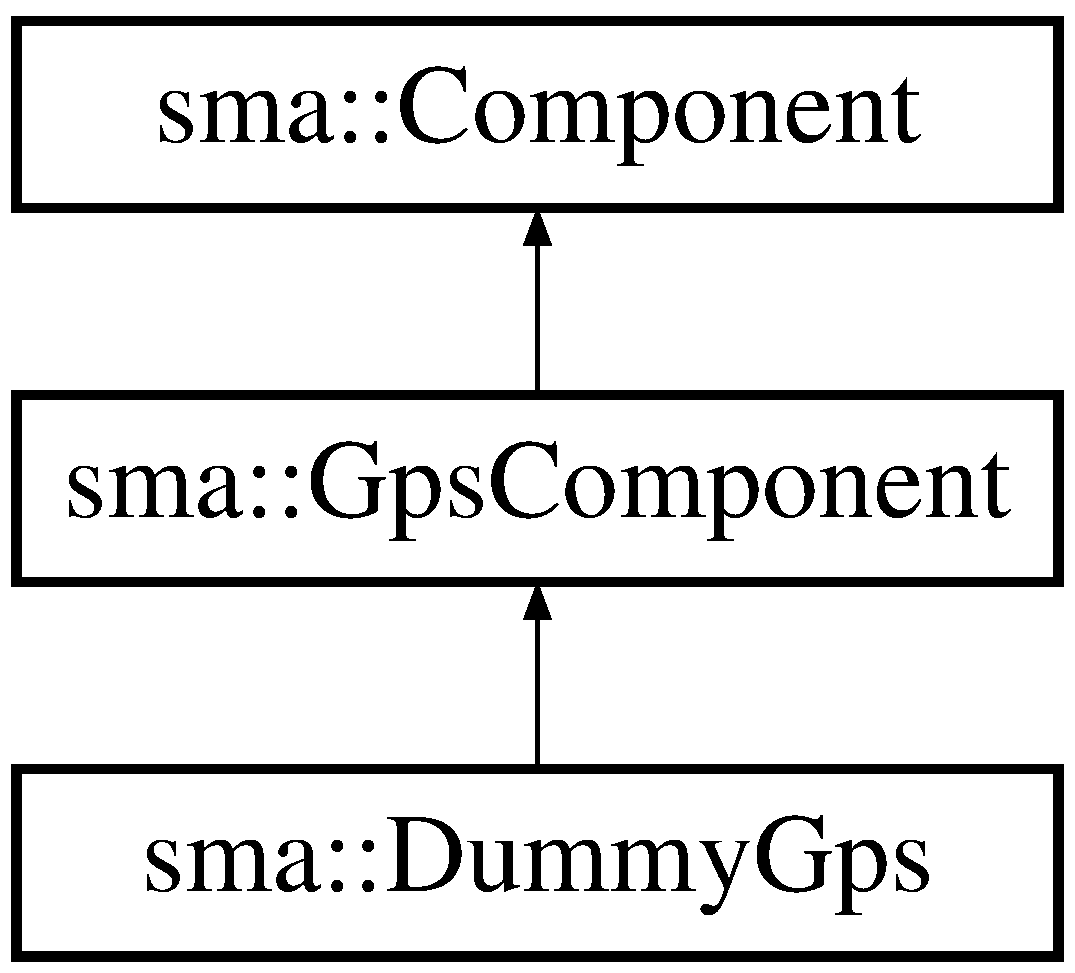
\includegraphics[height=3.000000cm]{classsma_1_1Component}
\end{center}
\end{figure}


The documentation for this class was generated from the following file\-:\begin{DoxyCompactItemize}
\item 
include/sma/component.\-hpp\end{DoxyCompactItemize}

\hypertarget{classel_1_1Configuration}{\section{el\-:\-:Configuration Class Reference}
\label{classel_1_1Configuration}\index{el\-::\-Configuration@{el\-::\-Configuration}}
}


Represents single configuration that has representing level, configuration type and a string based value.  




{\ttfamily \#include $<$logimpl.\-hpp$>$}

Inheritance diagram for el\-:\-:Configuration\-:\begin{figure}[H]
\begin{center}
\leavevmode
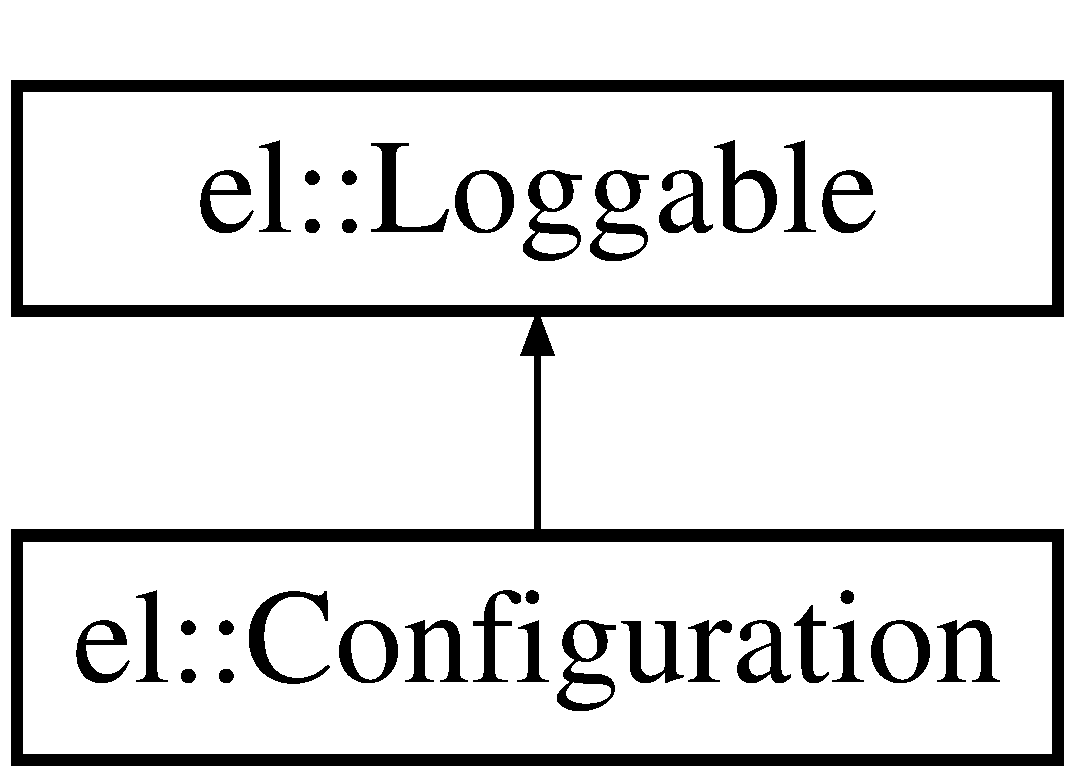
\includegraphics[height=2.000000cm]{classel_1_1Configuration}
\end{center}
\end{figure}
\subsection*{Classes}
\begin{DoxyCompactItemize}
\item 
class \hyperlink{classel_1_1Configuration_1_1Predicate}{Predicate}
\begin{DoxyCompactList}\small\item\em Used to find configuration from configuration (pointers) repository. Avoid using it. \end{DoxyCompactList}\end{DoxyCompactItemize}
\subsection*{Public Member Functions}
\begin{DoxyCompactItemize}
\item 
\hypertarget{classel_1_1Configuration_a71867a89e7d44cac62e0a436f01b484d}{{\bfseries Configuration} (const \hyperlink{classel_1_1Configuration}{Configuration} \&c)}\label{classel_1_1Configuration_a71867a89e7d44cac62e0a436f01b484d}

\item 
\hypertarget{classel_1_1Configuration_a80bc5b14f61906633cf695ea62e454a2}{\hyperlink{classel_1_1Configuration}{Configuration} \& {\bfseries operator=} (const \hyperlink{classel_1_1Configuration}{Configuration} \&c)}\label{classel_1_1Configuration_a80bc5b14f61906633cf695ea62e454a2}

\item 
\hypertarget{classel_1_1Configuration_a1a00abf955e028debaaf7556a647dbf5}{\hyperlink{classel_1_1Configuration_a1a00abf955e028debaaf7556a647dbf5}{Configuration} (\hyperlink{namespaceel_ab0ac6091262344c52dd2d3ad099e8e36}{Level} \hyperlink{classel_1_1Configuration_a66a96cf46d20204c50718f8a5e3622e2}{level}, \hyperlink{namespaceel_a281f5db6d6163678bc68a8b23b59e124}{Configuration\-Type} \hyperlink{classel_1_1Configuration_aab5091dcca176e309c0a2268ff55db0d}{configuration\-Type}, const std\-::string \&\hyperlink{classel_1_1Configuration_ab31605eb195a222cf32baa4922bb9a3c}{value})}\label{classel_1_1Configuration_a1a00abf955e028debaaf7556a647dbf5}

\begin{DoxyCompactList}\small\item\em Full constructor used to sets value of configuration. \end{DoxyCompactList}\item 
\hypertarget{classel_1_1Configuration_a66a96cf46d20204c50718f8a5e3622e2}{\hyperlink{namespaceel_ab0ac6091262344c52dd2d3ad099e8e36}{Level} \hyperlink{classel_1_1Configuration_a66a96cf46d20204c50718f8a5e3622e2}{level} (void) const }\label{classel_1_1Configuration_a66a96cf46d20204c50718f8a5e3622e2}

\begin{DoxyCompactList}\small\item\em Gets level of current configuration. \end{DoxyCompactList}\item 
\hypertarget{classel_1_1Configuration_aab5091dcca176e309c0a2268ff55db0d}{\hyperlink{namespaceel_a281f5db6d6163678bc68a8b23b59e124}{Configuration\-Type} \hyperlink{classel_1_1Configuration_aab5091dcca176e309c0a2268ff55db0d}{configuration\-Type} (void) const }\label{classel_1_1Configuration_aab5091dcca176e309c0a2268ff55db0d}

\begin{DoxyCompactList}\small\item\em Gets configuration type of current configuration. \end{DoxyCompactList}\item 
\hypertarget{classel_1_1Configuration_ab31605eb195a222cf32baa4922bb9a3c}{const std\-::string \& \hyperlink{classel_1_1Configuration_ab31605eb195a222cf32baa4922bb9a3c}{value} (void) const }\label{classel_1_1Configuration_ab31605eb195a222cf32baa4922bb9a3c}

\begin{DoxyCompactList}\small\item\em Gets string based configuration value. \end{DoxyCompactList}\item 
void \hyperlink{classel_1_1Configuration_a04755de11422d7570869433ea157b705}{set\-Value} (const std\-::string \&\hyperlink{classel_1_1Configuration_ab31605eb195a222cf32baa4922bb9a3c}{value})
\begin{DoxyCompactList}\small\item\em Set string based configuration value. \end{DoxyCompactList}\item 
\hypertarget{classel_1_1Configuration_a82c87e1a93211a1d21da99570f47dd49}{virtual void {\bfseries log} (el\-::base\-::type\-::ostream\-\_\-t \&os) const }\label{classel_1_1Configuration_a82c87e1a93211a1d21da99570f47dd49}

\end{DoxyCompactItemize}


\subsection{Detailed Description}
Represents single configuration that has representing level, configuration type and a string based value. 

String based value means any value either its boolean, integer or string itself, it will be embedded inside quotes and will be parsed later.

Consider some examples below\-:
\begin{DoxyItemize}
\item \hyperlink{classel_1_1Configuration}{el\-::\-Configuration} conf\-Enabled\-Info(\hyperlink{namespaceel_ab0ac6091262344c52dd2d3ad099e8e36a4059b0251f66a18cb56f544728796875}{el\-::\-Level\-::\-Info}, \hyperlink{namespaceel_a281f5db6d6163678bc68a8b23b59e124a00d23a76e43b46dae9ec7aa9dcbebb32}{el\-::\-Configuration\-Type\-::\-Enabled}, \char`\"{}true\char`\"{});
\item \hyperlink{classel_1_1Configuration}{el\-::\-Configuration} conf\-Max\-Log\-File\-Size\-Info(\hyperlink{namespaceel_ab0ac6091262344c52dd2d3ad099e8e36a4059b0251f66a18cb56f544728796875}{el\-::\-Level\-::\-Info}, \hyperlink{namespaceel_a281f5db6d6163678bc68a8b23b59e124a4b35e615142d60db6383426f051e700b}{el\-::\-Configuration\-Type\-::\-Max\-Log\-File\-Size}, \char`\"{}2048\char`\"{});
\item \hyperlink{classel_1_1Configuration}{el\-::\-Configuration} conf\-Filename\-Info(\hyperlink{namespaceel_ab0ac6091262344c52dd2d3ad099e8e36a4059b0251f66a18cb56f544728796875}{el\-::\-Level\-::\-Info}, \hyperlink{namespaceel_a281f5db6d6163678bc68a8b23b59e124a1351017ac6423911223bc19a8cb7c653}{el\-::\-Configuration\-Type\-::\-Filename}, \char`\"{}/var/log/my.\-log\char`\"{}); 
\end{DoxyItemize}

\subsection{Member Function Documentation}
\hypertarget{classel_1_1Configuration_a04755de11422d7570869433ea157b705}{\index{el\-::\-Configuration@{el\-::\-Configuration}!set\-Value@{set\-Value}}
\index{set\-Value@{set\-Value}!el::Configuration@{el\-::\-Configuration}}
\subsubsection[{set\-Value}]{\setlength{\rightskip}{0pt plus 5cm}void el\-::\-Configuration\-::set\-Value (
\begin{DoxyParamCaption}
\item[{const std\-::string \&}]{value}
\end{DoxyParamCaption}
)\hspace{0.3cm}{\ttfamily [inline]}}}\label{classel_1_1Configuration_a04755de11422d7570869433ea157b705}


Set string based configuration value. 


\begin{DoxyParams}{Parameters}
{\em value} & Value to set. Values have to be std\-::string; For boolean values use \char`\"{}true\char`\"{}, \char`\"{}false\char`\"{}, for any integral values use them in quotes. They will be parsed when configuring \\
\hline
\end{DoxyParams}


The documentation for this class was generated from the following file\-:\begin{DoxyCompactItemize}
\item 
include/sma/io/detail/logimpl.\-hpp\end{DoxyCompactItemize}

\hypertarget{classel_1_1Configurations}{\section{el\-:\-:Configurations Class Reference}
\label{classel_1_1Configurations}\index{el\-::\-Configurations@{el\-::\-Configurations}}
}


Thread-\/safe \hyperlink{classel_1_1Configuration}{Configuration} repository.  




{\ttfamily \#include $<$logimpl.\-hpp$>$}

Inheritance diagram for el\-:\-:Configurations\-:\begin{figure}[H]
\begin{center}
\leavevmode
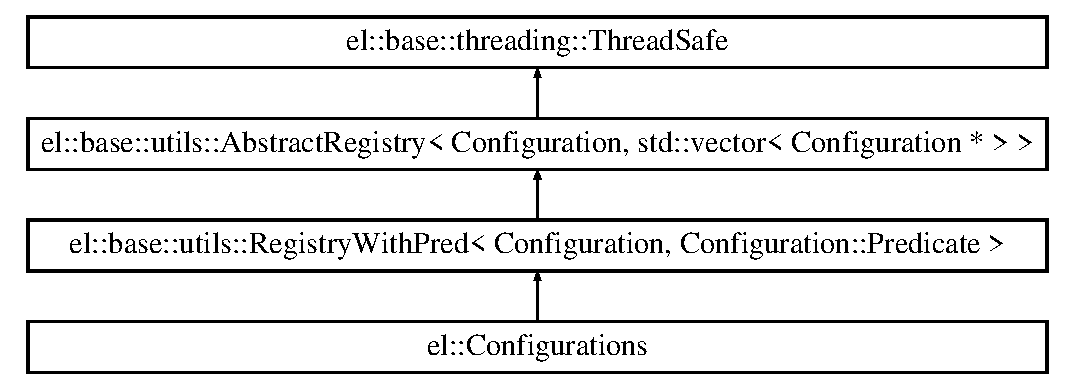
\includegraphics[height=4.000000cm]{classel_1_1Configurations}
\end{center}
\end{figure}
\subsection*{Classes}
\begin{DoxyCompactItemize}
\item 
class \hyperlink{classel_1_1Configurations_1_1Parser}{Parser}
\begin{DoxyCompactList}\small\item\em \hyperlink{classel_1_1Configurations_1_1Parser}{Parser} used internally to parse configurations from file or text. \end{DoxyCompactList}\end{DoxyCompactItemize}
\subsection*{Public Member Functions}
\begin{DoxyCompactItemize}
\item 
\hypertarget{classel_1_1Configurations_ae299dd1b60a1df9c013cc23029242a77}{\hyperlink{classel_1_1Configurations_ae299dd1b60a1df9c013cc23029242a77}{Configurations} (void)}\label{classel_1_1Configurations_ae299dd1b60a1df9c013cc23029242a77}

\begin{DoxyCompactList}\small\item\em Default constructor with empty repository. \end{DoxyCompactList}\item 
\hyperlink{classel_1_1Configurations_ae341bd647734d1180a5a138222d2f1ea}{Configurations} (const std\-::string \&\hyperlink{classel_1_1Configurations_a18df64bb5cd97bee672160290133141c}{configuration\-File}, bool use\-Defaults\-For\-Remaining=true, \hyperlink{classel_1_1Configurations}{Configurations} $\ast$base=nullptr)
\begin{DoxyCompactList}\small\item\em Constructor used to set configurations using configuration file. \end{DoxyCompactList}\item 
bool \hyperlink{classel_1_1Configurations_aaa098126d64a5ee04a3944b1a65dcdca}{parse\-From\-File} (const std\-::string \&\hyperlink{classel_1_1Configurations_a18df64bb5cd97bee672160290133141c}{configuration\-File}, \hyperlink{classel_1_1Configurations}{Configurations} $\ast$base=nullptr)
\begin{DoxyCompactList}\small\item\em Parses configuration from file. \end{DoxyCompactList}\item 
bool \hyperlink{classel_1_1Configurations_af262a41dff665a11889261137b62af4a}{parse\-From\-Text} (const std\-::string \&configurations\-String, \hyperlink{classel_1_1Configurations}{Configurations} $\ast$base=nullptr)
\begin{DoxyCompactList}\small\item\em Parse configurations from configuration string. \end{DoxyCompactList}\item 
void \hyperlink{classel_1_1Configurations_a4c6db218908b39d23cc09b1a16a18e83}{set\-From\-Base} (\hyperlink{classel_1_1Configurations}{Configurations} $\ast$base)
\begin{DoxyCompactList}\small\item\em Sets configuration based-\/off an existing configurations. \end{DoxyCompactList}\item 
bool \hyperlink{classel_1_1Configurations_a1e812370f896b6429bf46b31fcd4e3e0}{has\-Configuration} (\hyperlink{namespaceel_a281f5db6d6163678bc68a8b23b59e124}{Configuration\-Type} configuration\-Type)
\begin{DoxyCompactList}\small\item\em Determines whether or not specified configuration type exists in the repository. \end{DoxyCompactList}\item 
bool \hyperlink{classel_1_1Configurations_a5313557efac3b0c78f973a5a1d685277}{has\-Configuration} (\hyperlink{namespaceel_ab0ac6091262344c52dd2d3ad099e8e36}{Level} level, \hyperlink{namespaceel_a281f5db6d6163678bc68a8b23b59e124}{Configuration\-Type} configuration\-Type)
\begin{DoxyCompactList}\small\item\em Determines whether or not specified configuration type exists for specified level. \end{DoxyCompactList}\item 
void \hyperlink{classel_1_1Configurations_a332717de96efc851a202b7afcc5e395c}{set} (\hyperlink{namespaceel_ab0ac6091262344c52dd2d3ad099e8e36}{Level} level, \hyperlink{namespaceel_a281f5db6d6163678bc68a8b23b59e124}{Configuration\-Type} configuration\-Type, const std\-::string \&value)
\begin{DoxyCompactList}\small\item\em Sets value of configuration for specified level. \end{DoxyCompactList}\item 
void \hyperlink{classel_1_1Configurations_a0ab07520b9409fe9f2c16a705d6936f1}{set} (\hyperlink{classel_1_1Configuration}{Configuration} $\ast$conf)
\begin{DoxyCompactList}\small\item\em Sets single configuration based on other single configuration. \end{DoxyCompactList}\item 
\hypertarget{classel_1_1Configurations_a6da4bc9bd6a14dc44feaf25163e998ca}{\hyperlink{classel_1_1Configuration}{Configuration} $\ast$ {\bfseries get} (\hyperlink{namespaceel_ab0ac6091262344c52dd2d3ad099e8e36}{Level} level, \hyperlink{namespaceel_a281f5db6d6163678bc68a8b23b59e124}{Configuration\-Type} configuration\-Type)}\label{classel_1_1Configurations_a6da4bc9bd6a14dc44feaf25163e998ca}

\item 
void \hyperlink{classel_1_1Configurations_a56c82c15ea39cc230a5c85ec2c41cbfd}{set\-Globally} (\hyperlink{namespaceel_a281f5db6d6163678bc68a8b23b59e124}{Configuration\-Type} configuration\-Type, const std\-::string \&value)
\begin{DoxyCompactList}\small\item\em Sets configuration for all levels. \end{DoxyCompactList}\item 
\hypertarget{classel_1_1Configurations_a2a13be6154439286a68d2eccf8417edf}{void \hyperlink{classel_1_1Configurations_a2a13be6154439286a68d2eccf8417edf}{clear} (void)}\label{classel_1_1Configurations_a2a13be6154439286a68d2eccf8417edf}

\begin{DoxyCompactList}\small\item\em Clears repository so that all the configurations are unset. \end{DoxyCompactList}\item 
const std\-::string \& \hyperlink{classel_1_1Configurations_a18df64bb5cd97bee672160290133141c}{configuration\-File} (void) const 
\begin{DoxyCompactList}\small\item\em Gets configuration file used in parsing this configurations. \end{DoxyCompactList}\item 
\hypertarget{classel_1_1Configurations_ab34fa2ed4ac77f47b41e464c2d186239}{void \hyperlink{classel_1_1Configurations_ab34fa2ed4ac77f47b41e464c2d186239}{set\-To\-Default} (void)}\label{classel_1_1Configurations_ab34fa2ed4ac77f47b41e464c2d186239}

\begin{DoxyCompactList}\small\item\em Sets configurations to \char`\"{}factory based\char`\"{} configurations. \end{DoxyCompactList}\item 
void \hyperlink{classel_1_1Configurations_ad89b7d2dd750e4d1b3deff800e278fdb}{set\-Remaining\-To\-Default} (void)
\begin{DoxyCompactList}\small\item\em Lets you set the remaining configurations to default. \end{DoxyCompactList}\end{DoxyCompactItemize}
\subsection*{Friends}
\begin{DoxyCompactItemize}
\item 
\hypertarget{classel_1_1Configurations_a6efe246b312d02731fb0e1d120c0331d}{class {\bfseries el\-::\-Loggers}}\label{classel_1_1Configurations_a6efe246b312d02731fb0e1d120c0331d}

\end{DoxyCompactItemize}
\subsection*{Additional Inherited Members}


\subsection{Detailed Description}
Thread-\/safe \hyperlink{classel_1_1Configuration}{Configuration} repository. 

This repository represents configurations for all the levels and configuration type mapped to a value. 

\subsection{Constructor \& Destructor Documentation}
\hypertarget{classel_1_1Configurations_ae341bd647734d1180a5a138222d2f1ea}{\index{el\-::\-Configurations@{el\-::\-Configurations}!Configurations@{Configurations}}
\index{Configurations@{Configurations}!el::Configurations@{el\-::\-Configurations}}
\subsubsection[{Configurations}]{\setlength{\rightskip}{0pt plus 5cm}el\-::\-Configurations\-::\-Configurations (
\begin{DoxyParamCaption}
\item[{const std\-::string \&}]{configuration\-File, }
\item[{bool}]{use\-Defaults\-For\-Remaining = {\ttfamily true}, }
\item[{{\bf Configurations} $\ast$}]{base = {\ttfamily nullptr}}
\end{DoxyParamCaption}
)\hspace{0.3cm}{\ttfamily [inline]}}}\label{classel_1_1Configurations_ae341bd647734d1180a5a138222d2f1ea}


Constructor used to set configurations using configuration file. 


\begin{DoxyParams}{Parameters}
{\em configuration\-File} & Full path to configuration file \\
\hline
{\em use\-Defaults\-For\-Remaining} & Lets you set the remaining configurations to default. \\
\hline
{\em base} & If provided, this configuration will be based off existing repository that this argument is pointing to. \\
\hline
\end{DoxyParams}
\begin{DoxySeeAlso}{See Also}
\hyperlink{classel_1_1Configurations_aaa098126d64a5ee04a3944b1a65dcdca}{parse\-From\-File(const std\-::string\&, Configurations$\ast$ base)} 

\hyperlink{classel_1_1Configurations_ad89b7d2dd750e4d1b3deff800e278fdb}{set\-Remaining\-To\-Default()} 
\end{DoxySeeAlso}


\subsection{Member Function Documentation}
\hypertarget{classel_1_1Configurations_a18df64bb5cd97bee672160290133141c}{\index{el\-::\-Configurations@{el\-::\-Configurations}!configuration\-File@{configuration\-File}}
\index{configuration\-File@{configuration\-File}!el::Configurations@{el\-::\-Configurations}}
\subsubsection[{configuration\-File}]{\setlength{\rightskip}{0pt plus 5cm}const std\-::string\& el\-::\-Configurations\-::configuration\-File (
\begin{DoxyParamCaption}
\item[{void}]{}
\end{DoxyParamCaption}
) const\hspace{0.3cm}{\ttfamily [inline]}}}\label{classel_1_1Configurations_a18df64bb5cd97bee672160290133141c}


Gets configuration file used in parsing this configurations. 

If this repository was set manually or by text this returns empty string. \hypertarget{classel_1_1Configurations_a1e812370f896b6429bf46b31fcd4e3e0}{\index{el\-::\-Configurations@{el\-::\-Configurations}!has\-Configuration@{has\-Configuration}}
\index{has\-Configuration@{has\-Configuration}!el::Configurations@{el\-::\-Configurations}}
\subsubsection[{has\-Configuration}]{\setlength{\rightskip}{0pt plus 5cm}bool el\-::\-Configurations\-::has\-Configuration (
\begin{DoxyParamCaption}
\item[{{\bf Configuration\-Type}}]{configuration\-Type}
\end{DoxyParamCaption}
)\hspace{0.3cm}{\ttfamily [inline]}}}\label{classel_1_1Configurations_a1e812370f896b6429bf46b31fcd4e3e0}


Determines whether or not specified configuration type exists in the repository. 

Returns as soon as first level is found. 
\begin{DoxyParams}{Parameters}
{\em configuration\-Type} & Type of configuration to check existence for. \\
\hline
\end{DoxyParams}
\hypertarget{classel_1_1Configurations_a5313557efac3b0c78f973a5a1d685277}{\index{el\-::\-Configurations@{el\-::\-Configurations}!has\-Configuration@{has\-Configuration}}
\index{has\-Configuration@{has\-Configuration}!el::Configurations@{el\-::\-Configurations}}
\subsubsection[{has\-Configuration}]{\setlength{\rightskip}{0pt plus 5cm}bool el\-::\-Configurations\-::has\-Configuration (
\begin{DoxyParamCaption}
\item[{{\bf Level}}]{level, }
\item[{{\bf Configuration\-Type}}]{configuration\-Type}
\end{DoxyParamCaption}
)\hspace{0.3cm}{\ttfamily [inline]}}}\label{classel_1_1Configurations_a5313557efac3b0c78f973a5a1d685277}


Determines whether or not specified configuration type exists for specified level. 


\begin{DoxyParams}{Parameters}
{\em level} & Level to check \\
\hline
{\em configuration\-Type} & Type of configuration to check existence for. \\
\hline
\end{DoxyParams}
\hypertarget{classel_1_1Configurations_aaa098126d64a5ee04a3944b1a65dcdca}{\index{el\-::\-Configurations@{el\-::\-Configurations}!parse\-From\-File@{parse\-From\-File}}
\index{parse\-From\-File@{parse\-From\-File}!el::Configurations@{el\-::\-Configurations}}
\subsubsection[{parse\-From\-File}]{\setlength{\rightskip}{0pt plus 5cm}bool el\-::\-Configurations\-::parse\-From\-File (
\begin{DoxyParamCaption}
\item[{const std\-::string \&}]{configuration\-File, }
\item[{{\bf Configurations} $\ast$}]{base = {\ttfamily nullptr}}
\end{DoxyParamCaption}
)\hspace{0.3cm}{\ttfamily [inline]}}}\label{classel_1_1Configurations_aaa098126d64a5ee04a3944b1a65dcdca}


Parses configuration from file. 


\begin{DoxyParams}{Parameters}
{\em configuration\-File} & Full path to configuration file \\
\hline
{\em base} & \hyperlink{classel_1_1Configurations}{Configurations} to base new configuration repository off. This value is used when you want to use existing \hyperlink{classel_1_1Configurations}{Configurations} to base all the values and then set rest of configuration via configuration file. \\
\hline
\end{DoxyParams}
\begin{DoxyReturn}{Returns}
True if successfully parsed, false otherwise. You may define '\-\_\-\-E\-L\-P\-P\-\_\-\-D\-E\-B\-U\-G\-\_\-\-A\-S\-S\-E\-R\-T\-\_\-\-F\-A\-I\-L\-U\-R\-E' to make sure you do not proceed without successful parse. 
\end{DoxyReturn}
\hypertarget{classel_1_1Configurations_af262a41dff665a11889261137b62af4a}{\index{el\-::\-Configurations@{el\-::\-Configurations}!parse\-From\-Text@{parse\-From\-Text}}
\index{parse\-From\-Text@{parse\-From\-Text}!el::Configurations@{el\-::\-Configurations}}
\subsubsection[{parse\-From\-Text}]{\setlength{\rightskip}{0pt plus 5cm}bool el\-::\-Configurations\-::parse\-From\-Text (
\begin{DoxyParamCaption}
\item[{const std\-::string \&}]{configurations\-String, }
\item[{{\bf Configurations} $\ast$}]{base = {\ttfamily nullptr}}
\end{DoxyParamCaption}
)\hspace{0.3cm}{\ttfamily [inline]}}}\label{classel_1_1Configurations_af262a41dff665a11889261137b62af4a}


Parse configurations from configuration string. 

This configuration string has same syntax as configuration file contents. Make sure all the necessary new line characters are provided. 
\begin{DoxyParams}{Parameters}
{\em base} & \hyperlink{classel_1_1Configurations}{Configurations} to base new configuration repository off. This value is used when you want to use existing \hyperlink{classel_1_1Configurations}{Configurations} to base all the values and then set rest of configuration via configuration text. \\
\hline
\end{DoxyParams}
\begin{DoxyReturn}{Returns}
True if successfully parsed, false otherwise. You may define '\-\_\-\-E\-L\-P\-P\-\_\-\-D\-E\-B\-U\-G\-\_\-\-A\-S\-S\-E\-R\-T\-\_\-\-F\-A\-I\-L\-U\-R\-E' to make sure you do not proceed without successful parse. 
\end{DoxyReturn}
\hypertarget{classel_1_1Configurations_a332717de96efc851a202b7afcc5e395c}{\index{el\-::\-Configurations@{el\-::\-Configurations}!set@{set}}
\index{set@{set}!el::Configurations@{el\-::\-Configurations}}
\subsubsection[{set}]{\setlength{\rightskip}{0pt plus 5cm}void el\-::\-Configurations\-::set (
\begin{DoxyParamCaption}
\item[{{\bf Level}}]{level, }
\item[{{\bf Configuration\-Type}}]{configuration\-Type, }
\item[{const std\-::string \&}]{value}
\end{DoxyParamCaption}
)\hspace{0.3cm}{\ttfamily [inline]}}}\label{classel_1_1Configurations_a332717de96efc851a202b7afcc5e395c}


Sets value of configuration for specified level. 

Any existing configuration for specified level will be replaced. Also note that configuration types \hyperlink{namespaceel_a281f5db6d6163678bc68a8b23b59e124a052bf0f0c813b3c41c5b5046ebc26529}{Configuration\-Type\-::\-Milliseconds\-Width} and \hyperlink{namespaceel_a281f5db6d6163678bc68a8b23b59e124abe9e43d200c5698cb8519daed7035874}{Configuration\-Type\-::\-Performance\-Tracking} will be ignored if not set for \hyperlink{namespaceel_ab0ac6091262344c52dd2d3ad099e8e36a4cc6684df7b4a92b1dec6fce3264fac8}{Level\-::\-Global} because these configurations are not dependant on level. 
\begin{DoxyParams}{Parameters}
{\em level} & Level to set configuration for (\hyperlink{namespaceel_ab0ac6091262344c52dd2d3ad099e8e36}{el\-::\-Level}). \\
\hline
{\em configuration\-Type} & Type of configuration (\hyperlink{namespaceel_a281f5db6d6163678bc68a8b23b59e124}{el\-::\-Configuration\-Type}) \\
\hline
{\em value} & A string based value. Regardless of what the data type of configuration is, it will always be string from users' point of view. This is then parsed later to be used internally. \\
\hline
\end{DoxyParams}
\begin{DoxySeeAlso}{See Also}
\hyperlink{classel_1_1Configuration_a04755de11422d7570869433ea157b705}{Configuration\-::set\-Value(const std\-::string\& value)} 

\hyperlink{namespaceel_ab0ac6091262344c52dd2d3ad099e8e36}{el\-::\-Level} 

\hyperlink{namespaceel_a281f5db6d6163678bc68a8b23b59e124}{el\-::\-Configuration\-Type} 
\end{DoxySeeAlso}
\hypertarget{classel_1_1Configurations_a0ab07520b9409fe9f2c16a705d6936f1}{\index{el\-::\-Configurations@{el\-::\-Configurations}!set@{set}}
\index{set@{set}!el::Configurations@{el\-::\-Configurations}}
\subsubsection[{set}]{\setlength{\rightskip}{0pt plus 5cm}void el\-::\-Configurations\-::set (
\begin{DoxyParamCaption}
\item[{{\bf Configuration} $\ast$}]{conf}
\end{DoxyParamCaption}
)\hspace{0.3cm}{\ttfamily [inline]}}}\label{classel_1_1Configurations_a0ab07520b9409fe9f2c16a705d6936f1}


Sets single configuration based on other single configuration. 

\begin{DoxySeeAlso}{See Also}
\hyperlink{classel_1_1Configurations_a332717de96efc851a202b7afcc5e395c}{set}(\hyperlink{namespaceel_ab0ac6091262344c52dd2d3ad099e8e36}{Level} level, \hyperlink{namespaceel_a281f5db6d6163678bc68a8b23b59e124}{Configuration\-Type} configuration\-Type, const std\-::string\& value) 
\end{DoxySeeAlso}
\hypertarget{classel_1_1Configurations_a4c6db218908b39d23cc09b1a16a18e83}{\index{el\-::\-Configurations@{el\-::\-Configurations}!set\-From\-Base@{set\-From\-Base}}
\index{set\-From\-Base@{set\-From\-Base}!el::Configurations@{el\-::\-Configurations}}
\subsubsection[{set\-From\-Base}]{\setlength{\rightskip}{0pt plus 5cm}void el\-::\-Configurations\-::set\-From\-Base (
\begin{DoxyParamCaption}
\item[{{\bf Configurations} $\ast$}]{base}
\end{DoxyParamCaption}
)\hspace{0.3cm}{\ttfamily [inline]}}}\label{classel_1_1Configurations_a4c6db218908b39d23cc09b1a16a18e83}


Sets configuration based-\/off an existing configurations. 


\begin{DoxyParams}{Parameters}
{\em base} & Pointer to existing configurations. \\
\hline
\end{DoxyParams}
\hypertarget{classel_1_1Configurations_a56c82c15ea39cc230a5c85ec2c41cbfd}{\index{el\-::\-Configurations@{el\-::\-Configurations}!set\-Globally@{set\-Globally}}
\index{set\-Globally@{set\-Globally}!el::Configurations@{el\-::\-Configurations}}
\subsubsection[{set\-Globally}]{\setlength{\rightskip}{0pt plus 5cm}void el\-::\-Configurations\-::set\-Globally (
\begin{DoxyParamCaption}
\item[{{\bf Configuration\-Type}}]{configuration\-Type, }
\item[{const std\-::string \&}]{value}
\end{DoxyParamCaption}
)\hspace{0.3cm}{\ttfamily [inline]}}}\label{classel_1_1Configurations_a56c82c15ea39cc230a5c85ec2c41cbfd}


Sets configuration for all levels. 


\begin{DoxyParams}{Parameters}
{\em configuration\-Type} & Type of configuration \\
\hline
{\em value} & String based value \\
\hline
\end{DoxyParams}
\begin{DoxySeeAlso}{See Also}
\hyperlink{classel_1_1Configurations_a332717de96efc851a202b7afcc5e395c}{Configurations\-::set}(\hyperlink{namespaceel_ab0ac6091262344c52dd2d3ad099e8e36}{Level} level, \hyperlink{namespaceel_a281f5db6d6163678bc68a8b23b59e124}{Configuration\-Type} configuration\-Type, const std\-::string\& value) 
\end{DoxySeeAlso}
\hypertarget{classel_1_1Configurations_ad89b7d2dd750e4d1b3deff800e278fdb}{\index{el\-::\-Configurations@{el\-::\-Configurations}!set\-Remaining\-To\-Default@{set\-Remaining\-To\-Default}}
\index{set\-Remaining\-To\-Default@{set\-Remaining\-To\-Default}!el::Configurations@{el\-::\-Configurations}}
\subsubsection[{set\-Remaining\-To\-Default}]{\setlength{\rightskip}{0pt plus 5cm}void el\-::\-Configurations\-::set\-Remaining\-To\-Default (
\begin{DoxyParamCaption}
\item[{void}]{}
\end{DoxyParamCaption}
)\hspace{0.3cm}{\ttfamily [inline]}}}\label{classel_1_1Configurations_ad89b7d2dd750e4d1b3deff800e278fdb}


Lets you set the remaining configurations to default. 

By remaining, it means that the level/type a configuration does not exist for. This function is useful when you want to minimize chances of failures, e.\-g, if you have a configuration file that sets configuration for all the configurations except for Enabled or not, we use this so that E\-N\-A\-B\-L\-E\-D is set to default i.\-e, true. If you dont do this explicitley (either by calling this function or by using second param in Constructor and try to access a value, an error is thrown 

The documentation for this class was generated from the following file\-:\begin{DoxyCompactItemize}
\item 
include/sma/io/detail/logimpl.\-hpp\end{DoxyCompactItemize}

\hypertarget{classel_1_1ConfigurationTypeHelper}{\section{el\-:\-:Configuration\-Type\-Helper Class Reference}
\label{classel_1_1ConfigurationTypeHelper}\index{el\-::\-Configuration\-Type\-Helper@{el\-::\-Configuration\-Type\-Helper}}
}


Static class that contains helper functions for \hyperlink{namespaceel_a281f5db6d6163678bc68a8b23b59e124}{el\-::\-Configuration\-Type}.  




{\ttfamily \#include $<$logimpl.\-hpp$>$}

Inheritance diagram for el\-:\-:Configuration\-Type\-Helper\-:\begin{figure}[H]
\begin{center}
\leavevmode
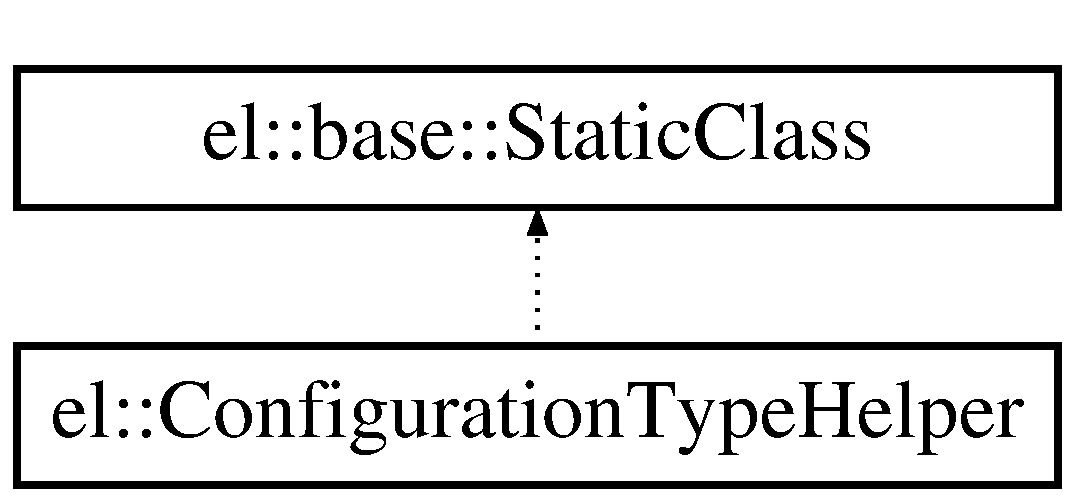
\includegraphics[height=2.000000cm]{classel_1_1ConfigurationTypeHelper}
\end{center}
\end{figure}
\subsection*{Static Public Member Functions}
\begin{DoxyCompactItemize}
\item 
\hypertarget{classel_1_1ConfigurationTypeHelper_aa53161071fee3ce3f371ab90c62d5fc2}{static base\-::type\-::\-Enum\-Type \hyperlink{classel_1_1ConfigurationTypeHelper_aa53161071fee3ce3f371ab90c62d5fc2}{cast\-To\-Int} (\hyperlink{namespaceel_a281f5db6d6163678bc68a8b23b59e124}{Configuration\-Type} configuration\-Type)}\label{classel_1_1ConfigurationTypeHelper_aa53161071fee3ce3f371ab90c62d5fc2}

\begin{DoxyCompactList}\small\item\em Casts configuration type to int, useful for iterating through enum. \end{DoxyCompactList}\item 
\hypertarget{classel_1_1ConfigurationTypeHelper_a62301cbc966cf7e7e2a7b55cc3259996}{static \hyperlink{namespaceel_a281f5db6d6163678bc68a8b23b59e124}{Configuration\-Type} \hyperlink{classel_1_1ConfigurationTypeHelper_a62301cbc966cf7e7e2a7b55cc3259996}{cast\-From\-Int} (base\-::type\-::\-Enum\-Type c)}\label{classel_1_1ConfigurationTypeHelper_a62301cbc966cf7e7e2a7b55cc3259996}

\begin{DoxyCompactList}\small\item\em Casts int(ushort) to configurationt type, useful for iterating through enum. \end{DoxyCompactList}\item 
static const char $\ast$ \hyperlink{classel_1_1ConfigurationTypeHelper_ad7f0a19c416c4a8ddaf85330b141383c}{convert\-To\-String} (\hyperlink{namespaceel_a281f5db6d6163678bc68a8b23b59e124}{Configuration\-Type} configuration\-Type)
\begin{DoxyCompactList}\small\item\em Converts configuration type to associated const char$\ast$. \end{DoxyCompactList}\item 
static \hyperlink{namespaceel_a281f5db6d6163678bc68a8b23b59e124}{Configuration\-Type} \hyperlink{classel_1_1ConfigurationTypeHelper_af4a35305e3941fd578e55fec624eba43}{convert\-From\-String} (const char $\ast$config\-Str)
\begin{DoxyCompactList}\small\item\em Converts from config\-Str to Configuration\-Type. \end{DoxyCompactList}\item 
static void \hyperlink{classel_1_1ConfigurationTypeHelper_ae5817d3d96672b15e813ebda1c9610f9}{for\-Each\-Config\-Type} (base\-::type\-::\-Enum\-Type $\ast$start\-Index, const std\-::function$<$ bool(void) $>$ \&fn)
\begin{DoxyCompactList}\small\item\em Applies specified function to each configuration type starting from start\-Index. \end{DoxyCompactList}\end{DoxyCompactItemize}
\subsection*{Static Public Attributes}
\begin{DoxyCompactItemize}
\item 
static const base\-::type\-::\-Enum\-Type \hyperlink{classel_1_1ConfigurationTypeHelper_ab7266e698eb32dec2da285325a66e322}{k\-Min\-Valid}
\begin{DoxyCompactList}\small\item\em Represents minimum valid configuration type. Useful when iterating through enum. \end{DoxyCompactList}\item 
static const base\-::type\-::\-Enum\-Type \hyperlink{classel_1_1ConfigurationTypeHelper_aa02f3cefb127e7eb97d7e1dd7f51a12d}{k\-Max\-Valid}
\begin{DoxyCompactList}\small\item\em Represents maximum valid configuration type. This is used internally and you should not need it. \end{DoxyCompactList}\end{DoxyCompactItemize}


\subsection{Detailed Description}
Static class that contains helper functions for \hyperlink{namespaceel_a281f5db6d6163678bc68a8b23b59e124}{el\-::\-Configuration\-Type}. 

\subsection{Member Function Documentation}
\hypertarget{classel_1_1ConfigurationTypeHelper_af4a35305e3941fd578e55fec624eba43}{\index{el\-::\-Configuration\-Type\-Helper@{el\-::\-Configuration\-Type\-Helper}!convert\-From\-String@{convert\-From\-String}}
\index{convert\-From\-String@{convert\-From\-String}!el::ConfigurationTypeHelper@{el\-::\-Configuration\-Type\-Helper}}
\subsubsection[{convert\-From\-String}]{\setlength{\rightskip}{0pt plus 5cm}static {\bf Configuration\-Type} el\-::\-Configuration\-Type\-Helper\-::convert\-From\-String (
\begin{DoxyParamCaption}
\item[{const char $\ast$}]{config\-Str}
\end{DoxyParamCaption}
)\hspace{0.3cm}{\ttfamily [inline]}, {\ttfamily [static]}}}\label{classel_1_1ConfigurationTypeHelper_af4a35305e3941fd578e55fec624eba43}


Converts from config\-Str to Configuration\-Type. 


\begin{DoxyParams}{Parameters}
{\em config\-Str} & Upper case string based configuration type. Lower case is also valid but providing upper case is recommended. \\
\hline
\end{DoxyParams}
\hypertarget{classel_1_1ConfigurationTypeHelper_ad7f0a19c416c4a8ddaf85330b141383c}{\index{el\-::\-Configuration\-Type\-Helper@{el\-::\-Configuration\-Type\-Helper}!convert\-To\-String@{convert\-To\-String}}
\index{convert\-To\-String@{convert\-To\-String}!el::ConfigurationTypeHelper@{el\-::\-Configuration\-Type\-Helper}}
\subsubsection[{convert\-To\-String}]{\setlength{\rightskip}{0pt plus 5cm}static const char$\ast$ el\-::\-Configuration\-Type\-Helper\-::convert\-To\-String (
\begin{DoxyParamCaption}
\item[{{\bf Configuration\-Type}}]{configuration\-Type}
\end{DoxyParamCaption}
)\hspace{0.3cm}{\ttfamily [inline]}, {\ttfamily [static]}}}\label{classel_1_1ConfigurationTypeHelper_ad7f0a19c416c4a8ddaf85330b141383c}


Converts configuration type to associated const char$\ast$. 

\begin{DoxyReturn}{Returns}
Upper case string based configuration type. 
\end{DoxyReturn}
\hypertarget{classel_1_1ConfigurationTypeHelper_ae5817d3d96672b15e813ebda1c9610f9}{\index{el\-::\-Configuration\-Type\-Helper@{el\-::\-Configuration\-Type\-Helper}!for\-Each\-Config\-Type@{for\-Each\-Config\-Type}}
\index{for\-Each\-Config\-Type@{for\-Each\-Config\-Type}!el::ConfigurationTypeHelper@{el\-::\-Configuration\-Type\-Helper}}
\subsubsection[{for\-Each\-Config\-Type}]{\setlength{\rightskip}{0pt plus 5cm}static void el\-::\-Configuration\-Type\-Helper\-::for\-Each\-Config\-Type (
\begin{DoxyParamCaption}
\item[{base\-::type\-::\-Enum\-Type $\ast$}]{start\-Index, }
\item[{const std\-::function$<$ bool(void) $>$ \&}]{fn}
\end{DoxyParamCaption}
)\hspace{0.3cm}{\ttfamily [inline]}, {\ttfamily [static]}}}\label{classel_1_1ConfigurationTypeHelper_ae5817d3d96672b15e813ebda1c9610f9}


Applies specified function to each configuration type starting from start\-Index. 


\begin{DoxyParams}{Parameters}
{\em start\-Index} & initial value to start the iteration from. This is passed by pointer and is left-\/shifted so this can be used inside function (fn) to represent current configuration type. \\
\hline
{\em fn} & function to apply with each configuration type. This bool represent whether or not to stop iterating through configurations. \\
\hline
\end{DoxyParams}


\subsection{Member Data Documentation}
\hypertarget{classel_1_1ConfigurationTypeHelper_aa02f3cefb127e7eb97d7e1dd7f51a12d}{\index{el\-::\-Configuration\-Type\-Helper@{el\-::\-Configuration\-Type\-Helper}!k\-Max\-Valid@{k\-Max\-Valid}}
\index{k\-Max\-Valid@{k\-Max\-Valid}!el::ConfigurationTypeHelper@{el\-::\-Configuration\-Type\-Helper}}
\subsubsection[{k\-Max\-Valid}]{\setlength{\rightskip}{0pt plus 5cm}const base\-::type\-::\-Enum\-Type el\-::\-Configuration\-Type\-Helper\-::k\-Max\-Valid\hspace{0.3cm}{\ttfamily [static]}}}\label{classel_1_1ConfigurationTypeHelper_aa02f3cefb127e7eb97d7e1dd7f51a12d}
{\bfseries Initial value\-:}
\begin{DoxyCode}
=
      \textcolor{keyword}{static\_cast<}base::type::EnumType\textcolor{keyword}{>}(\hyperlink{namespaceel_a281f5db6d6163678bc68a8b23b59e124a4b35e615142d60db6383426f051e700b}{ConfigurationType::MaxLogFileSize})
\end{DoxyCode}


Represents maximum valid configuration type. This is used internally and you should not need it. 

\hypertarget{classel_1_1ConfigurationTypeHelper_ab7266e698eb32dec2da285325a66e322}{\index{el\-::\-Configuration\-Type\-Helper@{el\-::\-Configuration\-Type\-Helper}!k\-Min\-Valid@{k\-Min\-Valid}}
\index{k\-Min\-Valid@{k\-Min\-Valid}!el::ConfigurationTypeHelper@{el\-::\-Configuration\-Type\-Helper}}
\subsubsection[{k\-Min\-Valid}]{\setlength{\rightskip}{0pt plus 5cm}const base\-::type\-::\-Enum\-Type el\-::\-Configuration\-Type\-Helper\-::k\-Min\-Valid\hspace{0.3cm}{\ttfamily [static]}}}\label{classel_1_1ConfigurationTypeHelper_ab7266e698eb32dec2da285325a66e322}
{\bfseries Initial value\-:}
\begin{DoxyCode}
=
      \textcolor{keyword}{static\_cast<}base::type::EnumType\textcolor{keyword}{>}(\hyperlink{namespaceel_a281f5db6d6163678bc68a8b23b59e124a00d23a76e43b46dae9ec7aa9dcbebb32}{ConfigurationType::Enabled})
\end{DoxyCode}


Represents minimum valid configuration type. Useful when iterating through enum. 



The documentation for this class was generated from the following file\-:\begin{DoxyCompactItemize}
\item 
include/sma/io/detail/logimpl.\-hpp\end{DoxyCompactItemize}

\hypertarget{structsma_1_1ContentAnnouncement}{\section{sma\-:\-:Content\-Announcement Struct Reference}
\label{structsma_1_1ContentAnnouncement}\index{sma\-::\-Content\-Announcement@{sma\-::\-Content\-Announcement}}
}
\subsection*{Public Member Functions}
\begin{DoxyCompactItemize}
\item 
\hypertarget{structsma_1_1ContentAnnouncement_aeeaadbe5d0f4378d4cde8c64aa2f0a54}{{\bfseries Content\-Announcement} (\hyperlink{structsma_1_1ContentDescriptor}{Content\-Descriptor} descriptor)}\label{structsma_1_1ContentAnnouncement_aeeaadbe5d0f4378d4cde8c64aa2f0a54}

\item 
\hypertarget{structsma_1_1ContentAnnouncement_a16a6fe90e1f97ac2a8c10054d41eeafd}{{\bfseries Content\-Announcement} (\hyperlink{structsma_1_1ContentAnnouncement}{Content\-Announcement} \&\&)=default}\label{structsma_1_1ContentAnnouncement_a16a6fe90e1f97ac2a8c10054d41eeafd}

\item 
\hypertarget{structsma_1_1ContentAnnouncement_a71a549f06568c621106b563bc8e60a0b}{{\bfseries Content\-Announcement} (\hyperlink{structsma_1_1ContentAnnouncement}{Content\-Announcement} const \&)=default}\label{structsma_1_1ContentAnnouncement_a71a549f06568c621106b563bc8e60a0b}

\item 
\hypertarget{structsma_1_1ContentAnnouncement_a32c0083cdefadeca2236166299586228}{\hyperlink{structsma_1_1ContentAnnouncement}{Content\-Announcement} \& {\bfseries operator=} (\hyperlink{structsma_1_1ContentAnnouncement}{Content\-Announcement} \&\&)=default}\label{structsma_1_1ContentAnnouncement_a32c0083cdefadeca2236166299586228}

\item 
\hypertarget{structsma_1_1ContentAnnouncement_a03a965794439f198285bf9e0e5ab6b34}{\hyperlink{structsma_1_1ContentAnnouncement}{Content\-Announcement} \& {\bfseries operator=} (\hyperlink{structsma_1_1ContentAnnouncement}{Content\-Announcement} const \&)=default}\label{structsma_1_1ContentAnnouncement_a03a965794439f198285bf9e0e5ab6b34}

\end{DoxyCompactItemize}
\subsection*{Public Attributes}
\begin{DoxyCompactItemize}
\item 
\hypertarget{structsma_1_1ContentAnnouncement_a4c5898183fab23c5c7964f18377da974}{\hyperlink{structsma_1_1ContentDescriptor}{Content\-Descriptor} {\bfseries descriptor}}\label{structsma_1_1ContentAnnouncement_a4c5898183fab23c5c7964f18377da974}

\end{DoxyCompactItemize}


The documentation for this struct was generated from the following file\-:\begin{DoxyCompactItemize}
\item 
include/sma/ccn/contentannouncement.\-hpp\end{DoxyCompactItemize}

\hypertarget{structsma_1_1ContentDescriptor}{\section{sma\-:\-:Content\-Descriptor Struct Reference}
\label{structsma_1_1ContentDescriptor}\index{sma\-::\-Content\-Descriptor@{sma\-::\-Content\-Descriptor}}
}


Content metadata descriptor for a single content item.  




{\ttfamily \#include $<$contentdescriptor.\-hpp$>$}

\subsection*{Public Types}
\begin{DoxyCompactItemize}
\item 
\hypertarget{structsma_1_1ContentDescriptor_a68b7045d54a2826abbd6fb6d393b77f3}{using {\bfseries time\-\_\-point} = clock\-::time\-\_\-point}\label{structsma_1_1ContentDescriptor_a68b7045d54a2826abbd6fb6d393b77f3}

\end{DoxyCompactItemize}
\subsection*{Public Member Functions}
\begin{DoxyCompactItemize}
\item 
\hypertarget{structsma_1_1ContentDescriptor_a65b2a03a56aa38d2eff2915a12c5fcdd}{{\bfseries T\-R\-I\-V\-I\-A\-L\-L\-Y\-\_\-\-S\-E\-R\-I\-A\-L\-I\-Z\-A\-B\-L\-E} (\hyperlink{structsma_1_1ContentDescriptor}{Content\-Descriptor}, hash, type, name, publisher, distance, \hyperlink{structsma_1_1ContentDescriptor_a5df5403d4d7e7a93ae3bf616f14eb598}{blocks}) using \hyperlink{structsma_1_1chrono_1_1system__clock}{clock}}\label{structsma_1_1ContentDescriptor_a65b2a03a56aa38d2eff2915a12c5fcdd}

\item 
\hypertarget{structsma_1_1ContentDescriptor_a7fab147dff32e4389e9293e19e8080ba}{{\bfseries Content\-Descriptor} (\hyperlink{structsma_1_1Hash}{Hash} hash, \hyperlink{structsma_1_1ContentType}{Content\-Type} type, \hyperlink{structsma_1_1ContentName}{Content\-Name} name, \hyperlink{structsma_1_1NodeId}{Node\-Id} publisher, std\-::vector$<$ \hyperlink{structsma_1_1Hash}{Hash} $>$ \hyperlink{structsma_1_1ContentDescriptor_a5df5403d4d7e7a93ae3bf616f14eb598}{blocks}=std\-::vector$<$ \hyperlink{structsma_1_1Hash}{Hash} $>$(), Network\-Distance distance=0)}\label{structsma_1_1ContentDescriptor_a7fab147dff32e4389e9293e19e8080ba}

\item 
\hypertarget{structsma_1_1ContentDescriptor_af9e1493085aa1666af655673abe97206}{bool {\bfseries update} (\hyperlink{structsma_1_1ContentDescriptor}{Content\-Descriptor} const \&info)}\label{structsma_1_1ContentDescriptor_af9e1493085aa1666af655673abe97206}

\end{DoxyCompactItemize}
\subsection*{Public Attributes}
\begin{DoxyCompactItemize}
\item 
\hypertarget{structsma_1_1ContentDescriptor_a79dbf0a252931a1da5f7bfcc241c5fb6}{\hyperlink{structsma_1_1Hash}{Hash} {\bfseries hash}}\label{structsma_1_1ContentDescriptor_a79dbf0a252931a1da5f7bfcc241c5fb6}

\item 
\hypertarget{structsma_1_1ContentDescriptor_a82ac4e52fb7d66e2a7fa0039ed10e20e}{\hyperlink{structsma_1_1ContentType}{Content\-Type} {\bfseries type}}\label{structsma_1_1ContentDescriptor_a82ac4e52fb7d66e2a7fa0039ed10e20e}

\item 
\hypertarget{structsma_1_1ContentDescriptor_ae2f7c491cafcc19dc497fb54c7ae0b18}{\hyperlink{structsma_1_1ContentName}{Content\-Name} {\bfseries name}}\label{structsma_1_1ContentDescriptor_ae2f7c491cafcc19dc497fb54c7ae0b18}

\item 
\hypertarget{structsma_1_1ContentDescriptor_a7f407c7636ff87a08ef17067b183d6f2}{\hyperlink{structsma_1_1NodeId}{Node\-Id} {\bfseries publisher}}\label{structsma_1_1ContentDescriptor_a7f407c7636ff87a08ef17067b183d6f2}

\item 
\hypertarget{structsma_1_1ContentDescriptor_ab874589ae9839fd5b9d26ecf89840f5b}{Network\-Distance {\bfseries distance}}\label{structsma_1_1ContentDescriptor_ab874589ae9839fd5b9d26ecf89840f5b}

\item 
\hypertarget{structsma_1_1ContentDescriptor_a5df5403d4d7e7a93ae3bf616f14eb598}{std\-::vector$<$ \hyperlink{structsma_1_1Hash}{Hash} $>$ \hyperlink{structsma_1_1ContentDescriptor_a5df5403d4d7e7a93ae3bf616f14eb598}{blocks}}\label{structsma_1_1ContentDescriptor_a5df5403d4d7e7a93ae3bf616f14eb598}

\begin{DoxyCompactList}\small\item\em The block set naming each block. \end{DoxyCompactList}\end{DoxyCompactItemize}


\subsection{Detailed Description}
Content metadata descriptor for a single content item. 

The descriptor must be sufficient to represent the content item's identity across network boundaries and to facilitate retrieval across node boundaries within the same application domain. 

The documentation for this struct was generated from the following file\-:\begin{DoxyCompactItemize}
\item 
include/sma/ccn/contentdescriptor.\-hpp\end{DoxyCompactItemize}

\hypertarget{classsma_1_1ContentHelper}{\section{sma\-:\-:Content\-Helper Class Reference}
\label{classsma_1_1ContentHelper}\index{sma\-::\-Content\-Helper@{sma\-::\-Content\-Helper}}
}
Inheritance diagram for sma\-:\-:Content\-Helper\-:\begin{figure}[H]
\begin{center}
\leavevmode
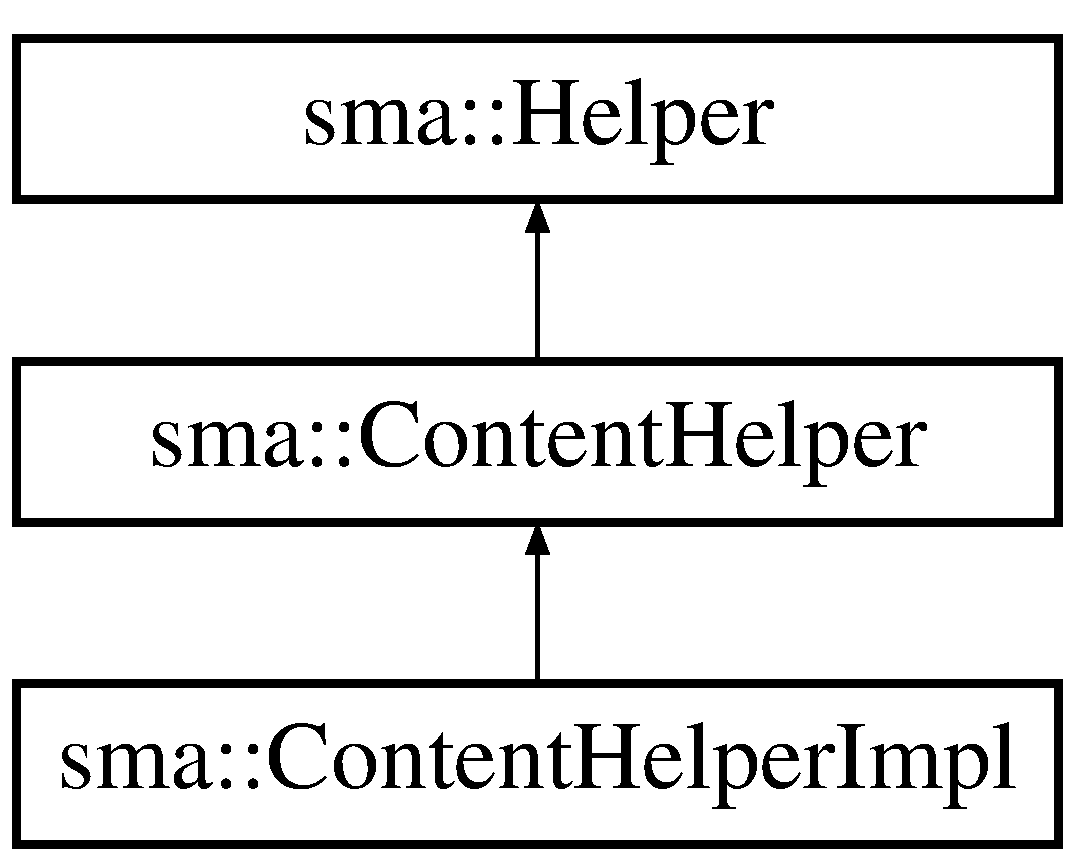
\includegraphics[height=3.000000cm]{classsma_1_1ContentHelper}
\end{center}
\end{figure}
\subsection*{Public Member Functions}
\begin{DoxyCompactItemize}
\item 
\hypertarget{classsma_1_1ContentHelper_a4885a081647b8d155b0b329cc41d7b27}{{\bfseries Content\-Helper} (\hyperlink{classsma_1_1CcnNode}{Ccn\-Node} \&node)}\label{classsma_1_1ContentHelper_a4885a081647b8d155b0b329cc41d7b27}

\item 
virtual void \hyperlink{classsma_1_1ContentHelper_ac19de65880beef7fa99a187945307d26}{receive} (\hyperlink{structsma_1_1MessageHeader}{Message\-Header} header, \hyperlink{structsma_1_1ContentAnnouncement}{Content\-Announcement} msg)=0
\begin{DoxyCompactList}\small\item\em Receive a content metadata announcement. \end{DoxyCompactList}\item 
virtual void \hyperlink{classsma_1_1ContentHelper_a8a17496e491d3996f93567821aef46b9}{publish} (\hyperlink{structsma_1_1ContentType}{Content\-Type} type, \hyperlink{structsma_1_1ContentName}{Content\-Name} name, std\-::istream \&is)=0
\end{DoxyCompactItemize}
\subsection*{Additional Inherited Members}


\subsection{Member Function Documentation}
\hypertarget{classsma_1_1ContentHelper_a8a17496e491d3996f93567821aef46b9}{\index{sma\-::\-Content\-Helper@{sma\-::\-Content\-Helper}!publish@{publish}}
\index{publish@{publish}!sma::ContentHelper@{sma\-::\-Content\-Helper}}
\subsubsection[{publish}]{\setlength{\rightskip}{0pt plus 5cm}virtual void sma\-::\-Content\-Helper\-::publish (
\begin{DoxyParamCaption}
\item[{{\bf Content\-Type}}]{type, }
\item[{{\bf Content\-Name}}]{name, }
\item[{std\-::istream \&}]{is}
\end{DoxyParamCaption}
)\hspace{0.3cm}{\ttfamily [pure virtual]}}}\label{classsma_1_1ContentHelper_a8a17496e491d3996f93567821aef46b9}
Store a piece of a content locally and broadcast a metadata announcement to the network. 

Implemented in \hyperlink{classsma_1_1ContentHelperImpl_a42163a01426a03d4517c245904aafbb3}{sma\-::\-Content\-Helper\-Impl}.

\hypertarget{classsma_1_1ContentHelper_ac19de65880beef7fa99a187945307d26}{\index{sma\-::\-Content\-Helper@{sma\-::\-Content\-Helper}!receive@{receive}}
\index{receive@{receive}!sma::ContentHelper@{sma\-::\-Content\-Helper}}
\subsubsection[{receive}]{\setlength{\rightskip}{0pt plus 5cm}virtual void sma\-::\-Content\-Helper\-::receive (
\begin{DoxyParamCaption}
\item[{{\bf Message\-Header}}]{header, }
\item[{{\bf Content\-Announcement}}]{msg}
\end{DoxyParamCaption}
)\hspace{0.3cm}{\ttfamily [pure virtual]}}}\label{classsma_1_1ContentHelper_ac19de65880beef7fa99a187945307d26}


Receive a content metadata announcement. 

A metadata announcement indicates that a piece of content is available from the publisher named in the metadata. The announcement may be forwarded so the publisher may be an undefined number of hops remote. 

Implemented in \hyperlink{classsma_1_1ContentHelperImpl_a0e4d3852c2c723e9e07242fa74738c63}{sma\-::\-Content\-Helper\-Impl}.



The documentation for this class was generated from the following files\-:\begin{DoxyCompactItemize}
\item 
include/sma/ccn/contenthelper.\-hpp\item 
src/ccn/contenthelper.\-cpp\end{DoxyCompactItemize}

\hypertarget{classsma_1_1ContentHelperImpl}{\section{sma\-:\-:Content\-Helper\-Impl Class Reference}
\label{classsma_1_1ContentHelperImpl}\index{sma\-::\-Content\-Helper\-Impl@{sma\-::\-Content\-Helper\-Impl}}
}


Manages the metadata, data, and traffic for content items in the network.  




{\ttfamily \#include $<$contenthelperimpl.\-hpp$>$}

Inheritance diagram for sma\-:\-:Content\-Helper\-Impl\-:\begin{figure}[H]
\begin{center}
\leavevmode
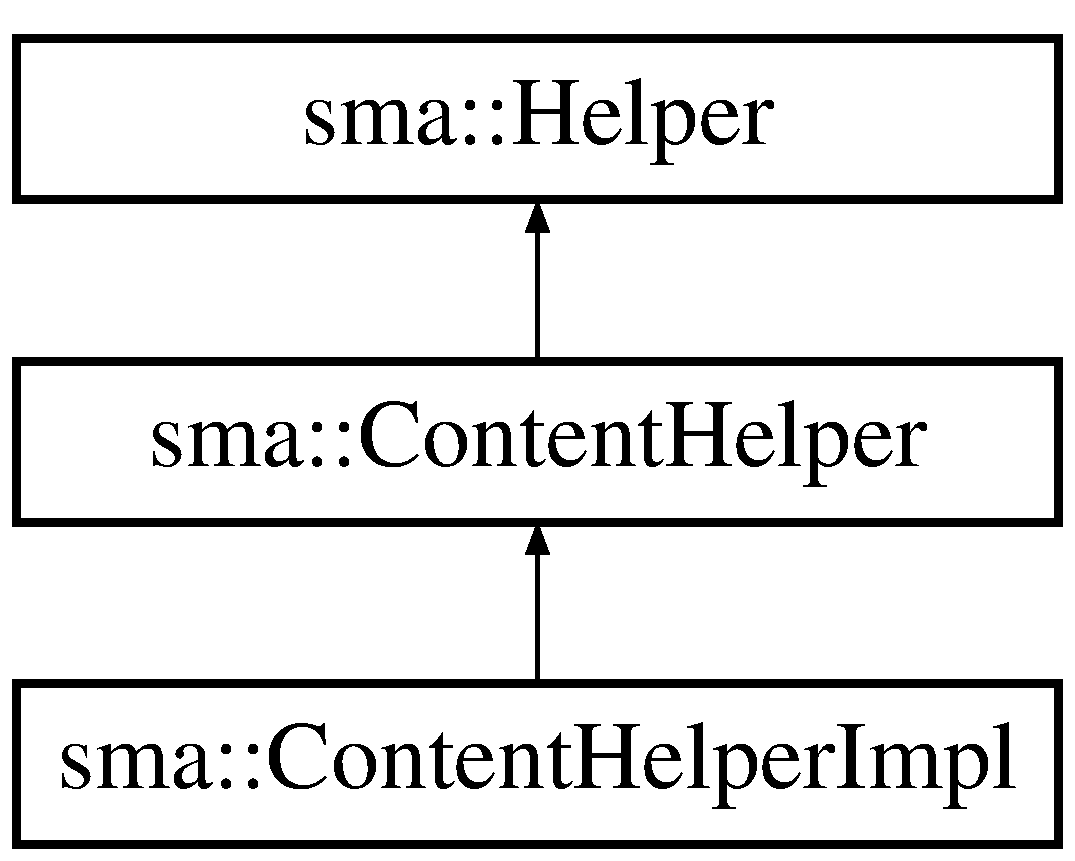
\includegraphics[height=3.000000cm]{classsma_1_1ContentHelperImpl}
\end{center}
\end{figure}
\subsection*{Public Member Functions}
\begin{DoxyCompactItemize}
\item 
\hypertarget{classsma_1_1ContentHelperImpl_a6a563ca7776e4bfe685113726e20f35c}{\hyperlink{classsma_1_1ContentHelperImpl_a6a563ca7776e4bfe685113726e20f35c}{Content\-Helper\-Impl} (\hyperlink{classsma_1_1CcnNode}{Ccn\-Node} \&node)}\label{classsma_1_1ContentHelperImpl_a6a563ca7776e4bfe685113726e20f35c}

\begin{DoxyCompactList}\small\item\em Construct a helper to manage the content for the given node. \end{DoxyCompactList}\item 
void \hyperlink{classsma_1_1ContentHelperImpl_a0e4d3852c2c723e9e07242fa74738c63}{receive} (\hyperlink{structsma_1_1MessageHeader}{Message\-Header} header, \hyperlink{structsma_1_1ContentAnnouncement}{Content\-Announcement} msg) override
\begin{DoxyCompactList}\small\item\em Receive a content metadata announcement. \end{DoxyCompactList}\item 
void \hyperlink{classsma_1_1ContentHelperImpl_a42163a01426a03d4517c245904aafbb3}{publish} (\hyperlink{structsma_1_1ContentType}{Content\-Type} type, \hyperlink{structsma_1_1ContentName}{Content\-Name} name, std\-::istream \&is) override
\end{DoxyCompactItemize}
\subsection*{Additional Inherited Members}


\subsection{Detailed Description}
Manages the metadata, data, and traffic for content items in the network. 

The content helper's responsibilities include publishing, storing, segmenting, caching, and replicating content and its metadata.

The helper does not manage interests as, though they do address the content, they do so only by reference and have no relation to its properties or behavior. 

\subsection{Member Function Documentation}
\hypertarget{classsma_1_1ContentHelperImpl_a42163a01426a03d4517c245904aafbb3}{\index{sma\-::\-Content\-Helper\-Impl@{sma\-::\-Content\-Helper\-Impl}!publish@{publish}}
\index{publish@{publish}!sma::ContentHelperImpl@{sma\-::\-Content\-Helper\-Impl}}
\subsubsection[{publish}]{\setlength{\rightskip}{0pt plus 5cm}void sma\-::\-Content\-Helper\-Impl\-::publish (
\begin{DoxyParamCaption}
\item[{{\bf Content\-Type}}]{type, }
\item[{{\bf Content\-Name}}]{name, }
\item[{std\-::istream \&}]{is}
\end{DoxyParamCaption}
)\hspace{0.3cm}{\ttfamily [override]}, {\ttfamily [virtual]}}}\label{classsma_1_1ContentHelperImpl_a42163a01426a03d4517c245904aafbb3}
Store a piece of a content locally and broadcast a metadata announcement to the network. 

Implements \hyperlink{classsma_1_1ContentHelper_a8a17496e491d3996f93567821aef46b9}{sma\-::\-Content\-Helper}.

\hypertarget{classsma_1_1ContentHelperImpl_a0e4d3852c2c723e9e07242fa74738c63}{\index{sma\-::\-Content\-Helper\-Impl@{sma\-::\-Content\-Helper\-Impl}!receive@{receive}}
\index{receive@{receive}!sma::ContentHelperImpl@{sma\-::\-Content\-Helper\-Impl}}
\subsubsection[{receive}]{\setlength{\rightskip}{0pt plus 5cm}void sma\-::\-Content\-Helper\-Impl\-::receive (
\begin{DoxyParamCaption}
\item[{{\bf Message\-Header}}]{header, }
\item[{{\bf Content\-Announcement}}]{msg}
\end{DoxyParamCaption}
)\hspace{0.3cm}{\ttfamily [override]}, {\ttfamily [virtual]}}}\label{classsma_1_1ContentHelperImpl_a0e4d3852c2c723e9e07242fa74738c63}


Receive a content metadata announcement. 

A metadata announcement indicates that a piece of content is available from the publisher named in the metadata. The announcement may be forwarded so the publisher may be an undefined number of hops remote. 

Implements \hyperlink{classsma_1_1ContentHelper_ac19de65880beef7fa99a187945307d26}{sma\-::\-Content\-Helper}.



The documentation for this class was generated from the following files\-:\begin{DoxyCompactItemize}
\item 
include/sma/ccn/contenthelperimpl.\-hpp\item 
src/ccn/contenthelperimpl.\-cpp\end{DoxyCompactItemize}

\hypertarget{structsma_1_1ContentName}{\section{sma\-:\-:Content\-Name Struct Reference}
\label{structsma_1_1ContentName}\index{sma\-::\-Content\-Name@{sma\-::\-Content\-Name}}
}
\subsection*{Public Member Functions}
\begin{DoxyCompactItemize}
\item 
\hypertarget{structsma_1_1ContentName_a8f520f18e5a0130d09c33958da8e7dca}{{\bfseries Content\-Name} (std\-::string value)}\label{structsma_1_1ContentName_a8f520f18e5a0130d09c33958da8e7dca}

\item 
\hypertarget{structsma_1_1ContentName_adfee7b94663265ccf0806931d31a7ce9}{bool {\bfseries operator==} (\hyperlink{structsma_1_1ContentName}{Content\-Name} const \&r) const }\label{structsma_1_1ContentName_adfee7b94663265ccf0806931d31a7ce9}

\item 
\hypertarget{structsma_1_1ContentName_a7ca47e366819a1fbfd7ee2c01a4aff39}{bool {\bfseries operator!=} (\hyperlink{structsma_1_1ContentName}{Content\-Name} const \&r) const }\label{structsma_1_1ContentName_a7ca47e366819a1fbfd7ee2c01a4aff39}

\item 
\hypertarget{structsma_1_1ContentName_ac07dc6f65ebb76d88cb2a789378cd37b}{bool {\bfseries operator$<$} (\hyperlink{structsma_1_1ContentName}{Content\-Name} const \&r) const }\label{structsma_1_1ContentName_ac07dc6f65ebb76d88cb2a789378cd37b}

\item 
\hypertarget{structsma_1_1ContentName_a2b815c3f0a12b7779771befde3a33ac2}{bool {\bfseries operator$>$} (\hyperlink{structsma_1_1ContentName}{Content\-Name} const \&r) const }\label{structsma_1_1ContentName_a2b815c3f0a12b7779771befde3a33ac2}

\item 
\hypertarget{structsma_1_1ContentName_ab277a3ad4e1c372f843c41d40e4d85e2}{bool {\bfseries operator$<$=} (\hyperlink{structsma_1_1ContentName}{Content\-Name} const \&r) const }\label{structsma_1_1ContentName_ab277a3ad4e1c372f843c41d40e4d85e2}

\item 
\hypertarget{structsma_1_1ContentName_a45ec3b085ccebf44c94f252731fdf0f2}{bool {\bfseries operator$>$=} (\hyperlink{structsma_1_1ContentName}{Content\-Name} const \&r) const }\label{structsma_1_1ContentName_a45ec3b085ccebf44c94f252731fdf0f2}

\item 
\hypertarget{structsma_1_1ContentName_a9b5cf4ca0f0aea27209feb257d6bd42a}{{\bfseries operator std\-::string} () const }\label{structsma_1_1ContentName_a9b5cf4ca0f0aea27209feb257d6bd42a}

\end{DoxyCompactItemize}
\subsection*{Friends}
\begin{DoxyCompactItemize}
\item 
\hypertarget{structsma_1_1ContentName_a1bfafb029481f0499f839a5361adada2}{struct {\bfseries std\-::hash$<$ Content\-Name $>$}}\label{structsma_1_1ContentName_a1bfafb029481f0499f839a5361adada2}

\end{DoxyCompactItemize}


The documentation for this struct was generated from the following file\-:\begin{DoxyCompactItemize}
\item 
include/sma/ccn/contentname.\-hpp\end{DoxyCompactItemize}

\hypertarget{classsma_1_1ContentStore}{\section{sma\-:\-:Content\-Store Class Reference}
\label{classsma_1_1ContentStore}\index{sma\-::\-Content\-Store@{sma\-::\-Content\-Store}}
}
Inheritance diagram for sma\-:\-:Content\-Store\-:\begin{figure}[H]
\begin{center}
\leavevmode
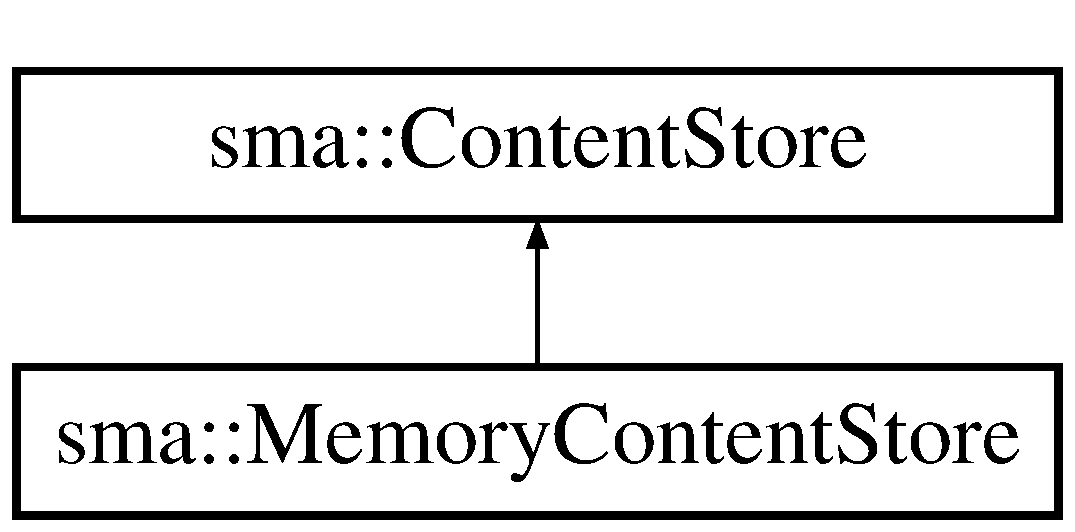
\includegraphics[height=2.000000cm]{classsma_1_1ContentStore}
\end{center}
\end{figure}
\subsection*{Public Member Functions}
\begin{DoxyCompactItemize}
\item 
\hypertarget{classsma_1_1ContentStore_a9f7e01764bfec2f75564a20fa7d1dc7f}{Stored\-Content {\bfseries store} (std\-::istream \&is)}\label{classsma_1_1ContentStore_a9f7e01764bfec2f75564a20fa7d1dc7f}

\end{DoxyCompactItemize}


The documentation for this class was generated from the following file\-:\begin{DoxyCompactItemize}
\item 
include/sma/ccn/contentstore.\-hpp\end{DoxyCompactItemize}

\hypertarget{structsma_1_1ContentType}{\section{sma\-:\-:Content\-Type Struct Reference}
\label{structsma_1_1ContentType}\index{sma\-::\-Content\-Type@{sma\-::\-Content\-Type}}
}
\subsection*{Public Member Functions}
\begin{DoxyCompactItemize}
\item 
\hypertarget{structsma_1_1ContentType_a7d23c0d130b7a08681f959ae78c54b29}{{\bfseries Content\-Type} (std\-::string value)}\label{structsma_1_1ContentType_a7d23c0d130b7a08681f959ae78c54b29}

\item 
\hypertarget{structsma_1_1ContentType_a4fe5d904675bae12d22c086319e534d0}{bool {\bfseries operator==} (\hyperlink{structsma_1_1ContentType}{Content\-Type} const \&r) const }\label{structsma_1_1ContentType_a4fe5d904675bae12d22c086319e534d0}

\item 
\hypertarget{structsma_1_1ContentType_af3237120b8772a43fe4e7021b729bcaa}{bool {\bfseries operator!=} (\hyperlink{structsma_1_1ContentType}{Content\-Type} const \&r) const }\label{structsma_1_1ContentType_af3237120b8772a43fe4e7021b729bcaa}

\item 
\hypertarget{structsma_1_1ContentType_aae340274f043e4739e09959cdf938ddd}{bool {\bfseries operator$<$} (\hyperlink{structsma_1_1ContentType}{Content\-Type} const \&r) const }\label{structsma_1_1ContentType_aae340274f043e4739e09959cdf938ddd}

\item 
\hypertarget{structsma_1_1ContentType_a267731f0fab65141d3ded72bc86073fc}{bool {\bfseries operator$>$} (\hyperlink{structsma_1_1ContentType}{Content\-Type} const \&r) const }\label{structsma_1_1ContentType_a267731f0fab65141d3ded72bc86073fc}

\item 
\hypertarget{structsma_1_1ContentType_a13d333cc3b49cc4f7ebaa5c548e1a743}{bool {\bfseries operator$<$=} (\hyperlink{structsma_1_1ContentType}{Content\-Type} const \&r) const }\label{structsma_1_1ContentType_a13d333cc3b49cc4f7ebaa5c548e1a743}

\item 
\hypertarget{structsma_1_1ContentType_aba39d4c5f587a79007970c737ee46c2b}{bool {\bfseries operator$>$=} (\hyperlink{structsma_1_1ContentType}{Content\-Type} const \&r) const }\label{structsma_1_1ContentType_aba39d4c5f587a79007970c737ee46c2b}

\item 
\hypertarget{structsma_1_1ContentType_a61ea9489436f81463d56d8b7e35b267b}{{\bfseries operator std\-::string} () const }\label{structsma_1_1ContentType_a61ea9489436f81463d56d8b7e35b267b}

\end{DoxyCompactItemize}
\subsection*{Friends}
\begin{DoxyCompactItemize}
\item 
\hypertarget{structsma_1_1ContentType_a59a19f82340a4eb90039408f1d900d21}{struct {\bfseries std\-::hash$<$ Content\-Type $>$}}\label{structsma_1_1ContentType_a59a19f82340a4eb90039408f1d900d21}

\end{DoxyCompactItemize}


The documentation for this struct was generated from the following file\-:\begin{DoxyCompactItemize}
\item 
include/sma/ccn/contenttype.\-hpp\end{DoxyCompactItemize}

\hypertarget{structsma_1_1Context}{\section{sma\-:\-:Context Struct Reference}
\label{structsma_1_1Context}\index{sma\-::\-Context@{sma\-::\-Context}}
}
\subsection*{Public Types}
\begin{DoxyCompactItemize}
\item 
\hypertarget{structsma_1_1Context_a0c156eea49d45224ed9704af320bbfff}{using {\bfseries prng\-\_\-type} = std\-::default\-\_\-random\-\_\-engine}\label{structsma_1_1Context_a0c156eea49d45224ed9704af320bbfff}

\item 
\hypertarget{structsma_1_1Context_ac00b1641d9bce206710bbd4014768489}{using {\bfseries prand\-\_\-value} = prng\-\_\-type\-::result\-\_\-type}\label{structsma_1_1Context_ac00b1641d9bce206710bbd4014768489}

\end{DoxyCompactItemize}
\subsection*{Public Member Functions}
\begin{DoxyCompactItemize}
\item 
\hypertarget{structsma_1_1Context_ae8754ff06a37b2b2a041336d1b0b2f90}{{\bfseries Context} (std\-::string name, \hyperlink{classsma_1_1LinkLayer}{Link\-Layer} \&linklayer)}\label{structsma_1_1Context_ae8754ff06a37b2b2a041336d1b0b2f90}

\item 
\hypertarget{structsma_1_1Context_a9f852acb4f4f0d0c6e671067459fad47}{{\bfseries Context} (\hyperlink{structsma_1_1Context}{Context} \&\&r)}\label{structsma_1_1Context_a9f852acb4f4f0d0c6e671067459fad47}

\item 
\hypertarget{structsma_1_1Context_a3c4bd983bcd0a5a070141713f51551f6}{\hyperlink{structsma_1_1Context}{Context} \& {\bfseries operator=} (\hyperlink{structsma_1_1Context}{Context} \&\&r)}\label{structsma_1_1Context_a3c4bd983bcd0a5a070141713f51551f6}

\item 
\hypertarget{structsma_1_1Context_a70044ab4744a375c2e93ed77a586b0ec}{void {\bfseries add\-\_\-component} (\hyperlink{classsma_1_1Component}{Component} \&c)}\label{structsma_1_1Context_a70044ab4744a375c2e93ed77a586b0ec}

\item 
\hypertarget{structsma_1_1Context_a93f795b66ad3dcdeff8592121f994764}{{\footnotesize template$<$typename T $>$ }\\T $\ast$ {\bfseries try\-\_\-get\-\_\-component} () const }\label{structsma_1_1Context_a93f795b66ad3dcdeff8592121f994764}

\item 
\hypertarget{structsma_1_1Context_a0dd07735a6cae9f43f0217abeebd5fd0}{prand\-\_\-value {\bfseries rand} ()}\label{structsma_1_1Context_a0dd07735a6cae9f43f0217abeebd5fd0}

\end{DoxyCompactItemize}
\subsection*{Public Attributes}
\begin{DoxyCompactItemize}
\item 
\hypertarget{structsma_1_1Context_a8884c30cbbd10b9121059156da57f03f}{prng\-\_\-type {\bfseries prng}}\label{structsma_1_1Context_a8884c30cbbd10b9121059156da57f03f}

\item 
\hypertarget{structsma_1_1Context_a33eacb080f9b3b17bfe032c15e6dbc0a}{\hyperlink{structsma_1_1Logger}{Logger} {\bfseries log}}\label{structsma_1_1Context_a33eacb080f9b3b17bfe032c15e6dbc0a}

\item 
\hypertarget{structsma_1_1Context_a7752557a3d9799e4b24086b9ea52e684}{\hyperlink{classsma_1_1LinkLayer}{Link\-Layer} $\ast$ {\bfseries linklayer}}\label{structsma_1_1Context_a7752557a3d9799e4b24086b9ea52e684}

\end{DoxyCompactItemize}


The documentation for this struct was generated from the following files\-:\begin{DoxyCompactItemize}
\item 
include/sma/context.\-hpp\item 
src/context.\-cpp\end{DoxyCompactItemize}

\hypertarget{structsma_1_1GPS_1_1Coord}{\section{sma\-:\-:G\-P\-S\-:\-:Coord Struct Reference}
\label{structsma_1_1GPS_1_1Coord}\index{sma\-::\-G\-P\-S\-::\-Coord@{sma\-::\-G\-P\-S\-::\-Coord}}
}
\subsection*{Public Member Functions}
\begin{DoxyCompactItemize}
\item 
\hypertarget{structsma_1_1GPS_1_1Coord_a58449254e9828e90d7c4d07e71d847d0}{{\bfseries Coord} (double lon, double lat)}\label{structsma_1_1GPS_1_1Coord_a58449254e9828e90d7c4d07e71d847d0}

\item 
\hypertarget{structsma_1_1GPS_1_1Coord_adf3d6c4b5e3885e05e892782b5d0a3c0}{double {\bfseries operator-\/} (\hyperlink{structsma_1_1GPS_1_1Coord}{Coord} const \&rhs)}\label{structsma_1_1GPS_1_1Coord_adf3d6c4b5e3885e05e892782b5d0a3c0}

\item 
\hypertarget{structsma_1_1GPS_1_1Coord_a83d6dc98c9058cec0f8fc59cefe293c0}{bool {\bfseries operator==} (\hyperlink{structsma_1_1GPS_1_1Coord}{Coord} const \&rhs)}\label{structsma_1_1GPS_1_1Coord_a83d6dc98c9058cec0f8fc59cefe293c0}

\item 
\hypertarget{structsma_1_1GPS_1_1Coord_a1dcb63bbd829fd964db09f46386e0873}{bool {\bfseries operator!=} (\hyperlink{structsma_1_1GPS_1_1Coord}{Coord} const \&rhs)}\label{structsma_1_1GPS_1_1Coord_a1dcb63bbd829fd964db09f46386e0873}

\end{DoxyCompactItemize}
\subsection*{Static Public Member Functions}
\begin{DoxyCompactItemize}
\item 
\hypertarget{structsma_1_1GPS_1_1Coord_acc89bcab41f37260ef108f5590224a6f}{static double {\bfseries dist} (\hyperlink{structsma_1_1GPS_1_1Coord}{Coord} const \&lhs, \hyperlink{structsma_1_1GPS_1_1Coord}{Coord} const \&rhs)}\label{structsma_1_1GPS_1_1Coord_acc89bcab41f37260ef108f5590224a6f}

\item 
\hypertarget{structsma_1_1GPS_1_1Coord_a2e322a3941d5168e25c30566385afe97}{static double {\bfseries dist\-\_\-sq} (\hyperlink{structsma_1_1GPS_1_1Coord}{Coord} const \&lhs, \hyperlink{structsma_1_1GPS_1_1Coord}{Coord} const \&rhs)}\label{structsma_1_1GPS_1_1Coord_a2e322a3941d5168e25c30566385afe97}

\end{DoxyCompactItemize}
\subsection*{Public Attributes}
\begin{DoxyCompactItemize}
\item 
\hypertarget{structsma_1_1GPS_1_1Coord_a7947a51769601b61c692ecb914915a73}{double {\bfseries lon}}\label{structsma_1_1GPS_1_1Coord_a7947a51769601b61c692ecb914915a73}

\item 
\hypertarget{structsma_1_1GPS_1_1Coord_a4803d065420279856f30c4a9a8c1bcc6}{double {\bfseries lat}}\label{structsma_1_1GPS_1_1Coord_a4803d065420279856f30c4a9a8c1bcc6}

\end{DoxyCompactItemize}


The documentation for this struct was generated from the following files\-:\begin{DoxyCompactItemize}
\item 
include/sma/gps.\-hpp\item 
src/gps.\-cpp\end{DoxyCompactItemize}

\hypertarget{classel_1_1base_1_1debug_1_1CrashHandler}{\section{el\-:\-:base\-:\-:debug\-:\-:Crash\-Handler Class Reference}
\label{classel_1_1base_1_1debug_1_1CrashHandler}\index{el\-::base\-::debug\-::\-Crash\-Handler@{el\-::base\-::debug\-::\-Crash\-Handler}}
}


Handles unexpected crashes.  




{\ttfamily \#include $<$logimpl.\-hpp$>$}

Inheritance diagram for el\-:\-:base\-:\-:debug\-:\-:Crash\-Handler\-:\begin{figure}[H]
\begin{center}
\leavevmode
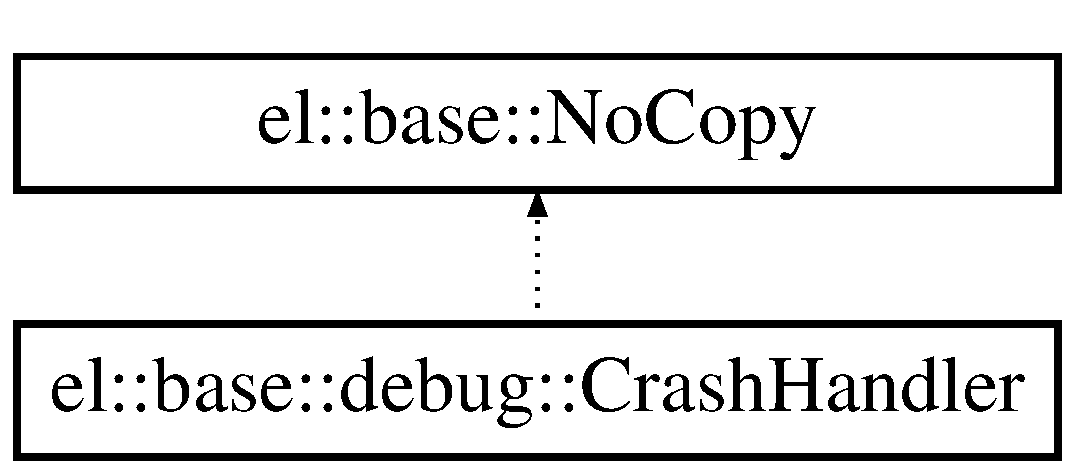
\includegraphics[height=2.000000cm]{classel_1_1base_1_1debug_1_1CrashHandler}
\end{center}
\end{figure}
\subsection*{Public Types}
\begin{DoxyCompactItemize}
\item 
\hypertarget{classel_1_1base_1_1debug_1_1CrashHandler_a838ba8e9b1587affca2b6cba02379cf1}{typedef void($\ast$ {\bfseries Handler} )(int)}\label{classel_1_1base_1_1debug_1_1CrashHandler_a838ba8e9b1587affca2b6cba02379cf1}

\end{DoxyCompactItemize}
\subsection*{Public Member Functions}
\begin{DoxyCompactItemize}
\item 
\hypertarget{classel_1_1base_1_1debug_1_1CrashHandler_a1d1e1a77bb6c37b1fbb39ecf94b38983}{{\bfseries Crash\-Handler} (bool use\-Default)}\label{classel_1_1base_1_1debug_1_1CrashHandler_a1d1e1a77bb6c37b1fbb39ecf94b38983}

\item 
\hypertarget{classel_1_1base_1_1debug_1_1CrashHandler_a9fbf8df7a292fcbeabfb87b241c83f78}{{\bfseries Crash\-Handler} (const Handler \&c\-Handler)}\label{classel_1_1base_1_1debug_1_1CrashHandler_a9fbf8df7a292fcbeabfb87b241c83f78}

\item 
\hypertarget{classel_1_1base_1_1debug_1_1CrashHandler_abd1d3d1ad5f1de2d40c39dd0542c26d4}{void {\bfseries set\-Handler} (const Handler \&c\-Handler)}\label{classel_1_1base_1_1debug_1_1CrashHandler_abd1d3d1ad5f1de2d40c39dd0542c26d4}

\end{DoxyCompactItemize}


\subsection{Detailed Description}
Handles unexpected crashes. 

The documentation for this class was generated from the following file\-:\begin{DoxyCompactItemize}
\item 
include/sma/io/detail/logimpl.\-hpp\end{DoxyCompactItemize}

\hypertarget{structsma_1_1CreateInterestAction}{\section{sma\-:\-:Create\-Interest\-Action Struct Reference}
\label{structsma_1_1CreateInterestAction}\index{sma\-::\-Create\-Interest\-Action@{sma\-::\-Create\-Interest\-Action}}
}
Inheritance diagram for sma\-:\-:Create\-Interest\-Action\-:\begin{figure}[H]
\begin{center}
\leavevmode
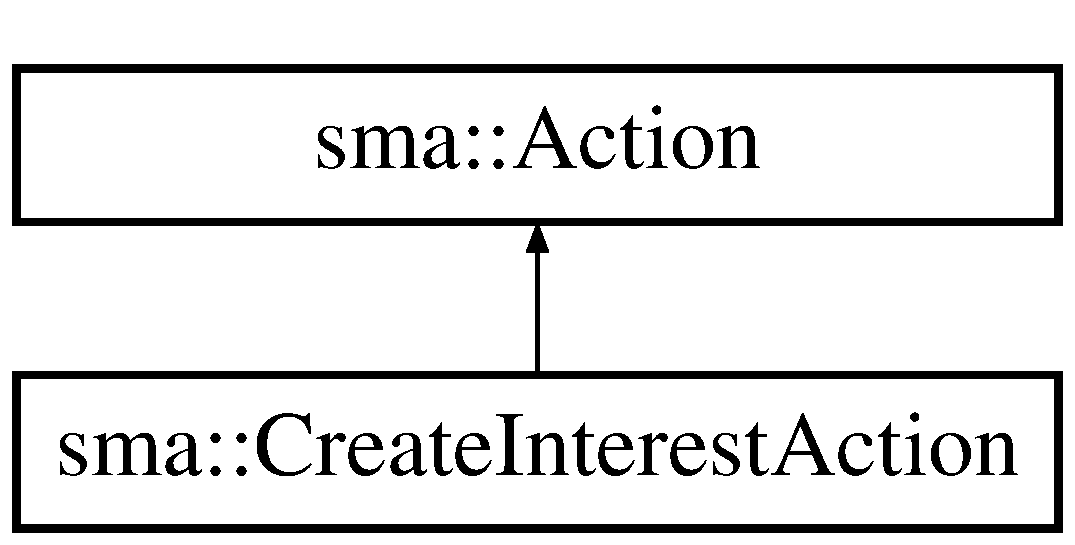
\includegraphics[height=2.000000cm]{structsma_1_1CreateInterestAction}
\end{center}
\end{figure}
\subsection*{Public Types}
\begin{DoxyCompactItemize}
\item 
\hypertarget{structsma_1_1CreateInterestAction_ab682f6a49bf3b6d659f127ba070d48f6}{using {\bfseries interests\-\_\-type} = std\-::vector$<$ \hyperlink{structsma_1_1ContentType}{Content\-Type} $>$}\label{structsma_1_1CreateInterestAction_ab682f6a49bf3b6d659f127ba070d48f6}

\end{DoxyCompactItemize}
\subsection*{Public Member Functions}
\begin{DoxyCompactItemize}
\item 
\hypertarget{structsma_1_1CreateInterestAction_ad9308248a7c5259da318b3a048ab1419}{{\bfseries Create\-Interest\-Action} (\hyperlink{classsma_1_1Ns3NodeContainer}{Ns3\-Node\-Container} \&context, interests\-\_\-type interests)}\label{structsma_1_1CreateInterestAction_ad9308248a7c5259da318b3a048ab1419}

\item 
\hypertarget{structsma_1_1CreateInterestAction_a52a88f8017244c251b84134ece0cc43c}{virtual void {\bfseries operator()} () override}\label{structsma_1_1CreateInterestAction_a52a88f8017244c251b84134ece0cc43c}

\end{DoxyCompactItemize}
\subsection*{Public Attributes}
\begin{DoxyCompactItemize}
\item 
\hypertarget{structsma_1_1CreateInterestAction_a4ebb99cb0958d70c29131434dcca78aa}{interests\-\_\-type {\bfseries interests}}\label{structsma_1_1CreateInterestAction_a4ebb99cb0958d70c29131434dcca78aa}

\end{DoxyCompactItemize}
\subsection*{Additional Inherited Members}


The documentation for this struct was generated from the following file\-:\begin{DoxyCompactItemize}
\item 
ns3/include/sma/ns3/createinterestaction.\-hpp\end{DoxyCompactItemize}

\hypertarget{classel_1_1CustomFormatSpecifier}{\section{el\-:\-:Custom\-Format\-Specifier Class Reference}
\label{classel_1_1CustomFormatSpecifier}\index{el\-::\-Custom\-Format\-Specifier@{el\-::\-Custom\-Format\-Specifier}}
}


User-\/provided custom format specifier.  




{\ttfamily \#include $<$logimpl.\-hpp$>$}

\subsection*{Public Member Functions}
\begin{DoxyCompactItemize}
\item 
\hypertarget{classel_1_1CustomFormatSpecifier_a1d1bfa8b489d2908ee543023a51e58f6}{{\bfseries Custom\-Format\-Specifier} (const char $\ast$format\-Specifier, const \hyperlink{namespaceel_a4d34c3ab99de9d5d2e531884d50bda3b}{Format\-Specifier\-Value\-Resolver} \&resolver)}\label{classel_1_1CustomFormatSpecifier_a1d1bfa8b489d2908ee543023a51e58f6}

\item 
\hypertarget{classel_1_1CustomFormatSpecifier_a0be00787b7ca1caedd32e1627d76fd24}{const char $\ast$ {\bfseries format\-Specifier} (void) const }\label{classel_1_1CustomFormatSpecifier_a0be00787b7ca1caedd32e1627d76fd24}

\item 
\hypertarget{classel_1_1CustomFormatSpecifier_ac426e6771ae35e060313b8683b88adc8}{const \\*
\hyperlink{namespaceel_a4d34c3ab99de9d5d2e531884d50bda3b}{Format\-Specifier\-Value\-Resolver} \& {\bfseries resolver} (void) const }\label{classel_1_1CustomFormatSpecifier_ac426e6771ae35e060313b8683b88adc8}

\item 
\hypertarget{classel_1_1CustomFormatSpecifier_ae17a9fbf8c5a28867308fcb8966a3aa0}{bool {\bfseries operator==} (const char $\ast$format\-Specifier)}\label{classel_1_1CustomFormatSpecifier_ae17a9fbf8c5a28867308fcb8966a3aa0}

\end{DoxyCompactItemize}


\subsection{Detailed Description}
User-\/provided custom format specifier. 

\begin{DoxySeeAlso}{See Also}
\hyperlink{classel_1_1Helpers_aa6de15a09db4f2a6763a6652c0ea12b1}{el\-::\-Helpers\-::install\-Custom\-Format\-Specifier} 

\hyperlink{namespaceel_a4d34c3ab99de9d5d2e531884d50bda3b}{Format\-Specifier\-Value\-Resolver} 
\end{DoxySeeAlso}


The documentation for this class was generated from the following file\-:\begin{DoxyCompactItemize}
\item 
include/sma/io/detail/logimpl.\-hpp\end{DoxyCompactItemize}

\hypertarget{classsma_1_1cyclic__barrier}{\section{sma\-:\-:cyclic\-\_\-barrier Class Reference}
\label{classsma_1_1cyclic__barrier}\index{sma\-::cyclic\-\_\-barrier@{sma\-::cyclic\-\_\-barrier}}
}
\subsection*{Public Member Functions}
\begin{DoxyCompactItemize}
\item 
\hypertarget{classsma_1_1cyclic__barrier_a7229a41e241bc8efa20a0af724ee2622}{{\bfseries cyclic\-\_\-barrier} (std\-::size\-\_\-t nthreads)}\label{classsma_1_1cyclic__barrier_a7229a41e241bc8efa20a0af724ee2622}

\item 
\hypertarget{classsma_1_1cyclic__barrier_a57d39d4ed0a651c22d6690a31adc8a05}{{\bfseries cyclic\-\_\-barrier} (std\-::size\-\_\-t nthreads, std\-::function$<$ void()$>$ \&\&on\-\_\-open)}\label{classsma_1_1cyclic__barrier_a57d39d4ed0a651c22d6690a31adc8a05}

\item 
\hypertarget{classsma_1_1cyclic__barrier_a870cbe42f23d9116c4e178f4acc77f79}{void {\bfseries wait} ()}\label{classsma_1_1cyclic__barrier_a870cbe42f23d9116c4e178f4acc77f79}

\end{DoxyCompactItemize}


The documentation for this class was generated from the following file\-:\begin{DoxyCompactItemize}
\item 
include/sma/concurrent/cyclic\-\_\-barrier.\-hpp\end{DoxyCompactItemize}

\hypertarget{classel_1_1base_1_1utils_1_1DateTime}{\section{el\-:\-:base\-:\-:utils\-:\-:Date\-Time Class Reference}
\label{classel_1_1base_1_1utils_1_1DateTime}\index{el\-::base\-::utils\-::\-Date\-Time@{el\-::base\-::utils\-::\-Date\-Time}}
}


Contains utilities for cross-\/platform date/time. This class make use of \hyperlink{classel_1_1base_1_1utils_1_1Str}{el\-::base\-::utils\-::\-Str}.  




{\ttfamily \#include $<$logimpl.\-hpp$>$}

Inheritance diagram for el\-:\-:base\-:\-:utils\-:\-:Date\-Time\-:\begin{figure}[H]
\begin{center}
\leavevmode
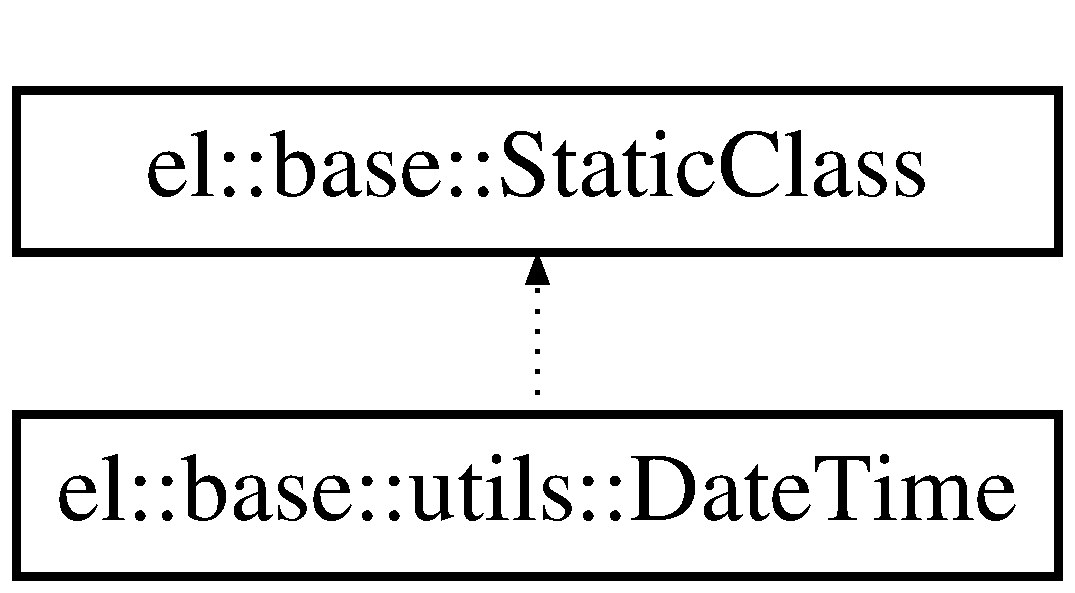
\includegraphics[height=2.000000cm]{classel_1_1base_1_1utils_1_1DateTime}
\end{center}
\end{figure}
\subsection*{Static Public Member Functions}
\begin{DoxyCompactItemize}
\item 
static void \hyperlink{classel_1_1base_1_1utils_1_1DateTime_ac000e6ecf705c2194a173d618ff4acfd}{gettimeofday} (struct timeval $\ast$tv)
\begin{DoxyCompactList}\small\item\em Cross platform gettimeofday for Windows and unix platform. This can be used to determine current millisecond. \end{DoxyCompactList}\item 
static std\-::string \hyperlink{classel_1_1base_1_1utils_1_1DateTime_aa813c606a98b8741f59ccdf5aacef733}{get\-Date\-Time} (const char $\ast$format, const \hyperlink{classel_1_1base_1_1MillisecondsWidth}{base\-::\-Milliseconds\-Width} $\ast$ms\-Width)
\begin{DoxyCompactList}\small\item\em Gets current date and time with milliseconds. \end{DoxyCompactList}\item 
\hypertarget{classel_1_1base_1_1utils_1_1DateTime_a1eea58fffe291c969a526d08515d29d7}{static base\-::type\-::string\-\_\-t \hyperlink{classel_1_1base_1_1utils_1_1DateTime_a1eea58fffe291c969a526d08515d29d7}{format\-Time} (unsigned long long time, \hyperlink{namespaceel_1_1base_a1b886858c6409097395b24b1bdf03c39}{base\-::\-Timestamp\-Unit} timestamp\-Unit)}\label{classel_1_1base_1_1utils_1_1DateTime_a1eea58fffe291c969a526d08515d29d7}

\begin{DoxyCompactList}\small\item\em Formats time to get unit accordingly, units like second if $>$ 1000 or minutes if $>$ 60000 etc. \end{DoxyCompactList}\item 
\hypertarget{classel_1_1base_1_1utils_1_1DateTime_a9181a3544442e1d3c05d8c96bbfff16d}{static unsigned long long \hyperlink{classel_1_1base_1_1utils_1_1DateTime_a9181a3544442e1d3c05d8c96bbfff16d}{get\-Time\-Difference} (const struct timeval \&end\-Time, const struct timeval \&start\-Time, \hyperlink{namespaceel_1_1base_a1b886858c6409097395b24b1bdf03c39}{base\-::\-Timestamp\-Unit} timestamp\-Unit)}\label{classel_1_1base_1_1utils_1_1DateTime_a9181a3544442e1d3c05d8c96bbfff16d}

\begin{DoxyCompactList}\small\item\em Gets time difference in milli/micro second depending on timestamp\-Unit. \end{DoxyCompactList}\end{DoxyCompactItemize}


\subsection{Detailed Description}
Contains utilities for cross-\/platform date/time. This class make use of \hyperlink{classel_1_1base_1_1utils_1_1Str}{el\-::base\-::utils\-::\-Str}. 

\subsection{Member Function Documentation}
\hypertarget{classel_1_1base_1_1utils_1_1DateTime_aa813c606a98b8741f59ccdf5aacef733}{\index{el\-::base\-::utils\-::\-Date\-Time@{el\-::base\-::utils\-::\-Date\-Time}!get\-Date\-Time@{get\-Date\-Time}}
\index{get\-Date\-Time@{get\-Date\-Time}!el::base::utils::DateTime@{el\-::base\-::utils\-::\-Date\-Time}}
\subsubsection[{get\-Date\-Time}]{\setlength{\rightskip}{0pt plus 5cm}static std\-::string el\-::base\-::utils\-::\-Date\-Time\-::get\-Date\-Time (
\begin{DoxyParamCaption}
\item[{const char $\ast$}]{format, }
\item[{const {\bf base\-::\-Milliseconds\-Width} $\ast$}]{ms\-Width}
\end{DoxyParamCaption}
)\hspace{0.3cm}{\ttfamily [inline]}, {\ttfamily [static]}}}\label{classel_1_1base_1_1utils_1_1DateTime_aa813c606a98b8741f59ccdf5aacef733}


Gets current date and time with milliseconds. 


\begin{DoxyParams}{Parameters}
{\em format} & User provided date/time format \\
\hline
{\em ms\-Width} & A pointer to \hyperlink{classel_1_1base_1_1MillisecondsWidth}{base\-::\-Milliseconds\-Width} from configuration (non-\/null) \\
\hline
\end{DoxyParams}
\begin{DoxyReturn}{Returns}
string based date time in specified format. 
\end{DoxyReturn}
\hypertarget{classel_1_1base_1_1utils_1_1DateTime_ac000e6ecf705c2194a173d618ff4acfd}{\index{el\-::base\-::utils\-::\-Date\-Time@{el\-::base\-::utils\-::\-Date\-Time}!gettimeofday@{gettimeofday}}
\index{gettimeofday@{gettimeofday}!el::base::utils::DateTime@{el\-::base\-::utils\-::\-Date\-Time}}
\subsubsection[{gettimeofday}]{\setlength{\rightskip}{0pt plus 5cm}static void el\-::base\-::utils\-::\-Date\-Time\-::gettimeofday (
\begin{DoxyParamCaption}
\item[{struct timeval $\ast$}]{tv}
\end{DoxyParamCaption}
)\hspace{0.3cm}{\ttfamily [inline]}, {\ttfamily [static]}}}\label{classel_1_1base_1_1utils_1_1DateTime_ac000e6ecf705c2194a173d618ff4acfd}


Cross platform gettimeofday for Windows and unix platform. This can be used to determine current millisecond. 

For unix system it uses gettimeofday(timeval$\ast$, timezone$\ast$) and for Windows, a seperate implementation is provided 
\begin{DoxyParams}[1]{Parameters}
\mbox{\tt in,out}  & {\em tv} & Pointer that gets updated \\
\hline
\end{DoxyParams}


The documentation for this class was generated from the following file\-:\begin{DoxyCompactItemize}
\item 
include/sma/io/detail/logimpl.\-hpp\end{DoxyCompactItemize}

\hypertarget{classel_1_1base_1_1DefaultLogBuilder}{\section{el\-:\-:base\-:\-:Default\-Log\-Builder Class Reference}
\label{classel_1_1base_1_1DefaultLogBuilder}\index{el\-::base\-::\-Default\-Log\-Builder@{el\-::base\-::\-Default\-Log\-Builder}}
}
Inheritance diagram for el\-:\-:base\-:\-:Default\-Log\-Builder\-:\begin{figure}[H]
\begin{center}
\leavevmode
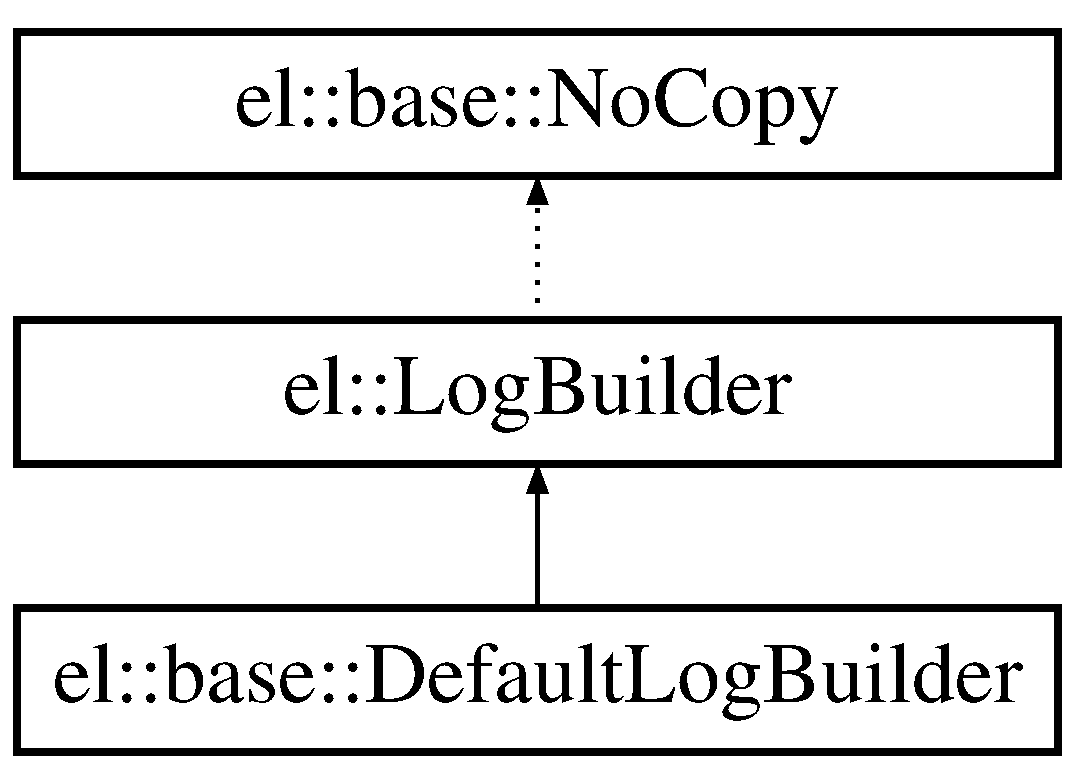
\includegraphics[height=3.000000cm]{classel_1_1base_1_1DefaultLogBuilder}
\end{center}
\end{figure}
\subsection*{Public Member Functions}
\begin{DoxyCompactItemize}
\item 
\hypertarget{classel_1_1base_1_1DefaultLogBuilder_aa8d2f42068115d899ed81de1b0ed360e}{base\-::type\-::string\-\_\-t {\bfseries build} (const \hyperlink{classel_1_1LogMessage}{Log\-Message} $\ast$log\-Message, bool append\-New\-Line) const }\label{classel_1_1base_1_1DefaultLogBuilder_aa8d2f42068115d899ed81de1b0ed360e}

\end{DoxyCompactItemize}


The documentation for this class was generated from the following file\-:\begin{DoxyCompactItemize}
\item 
include/sma/io/detail/logimpl.\-hpp\end{DoxyCompactItemize}

\hypertarget{classel_1_1base_1_1DefaultLogDispatchCallback}{\section{el\-:\-:base\-:\-:Default\-Log\-Dispatch\-Callback Class Reference}
\label{classel_1_1base_1_1DefaultLogDispatchCallback}\index{el\-::base\-::\-Default\-Log\-Dispatch\-Callback@{el\-::base\-::\-Default\-Log\-Dispatch\-Callback}}
}
Inheritance diagram for el\-:\-:base\-:\-:Default\-Log\-Dispatch\-Callback\-:\begin{figure}[H]
\begin{center}
\leavevmode
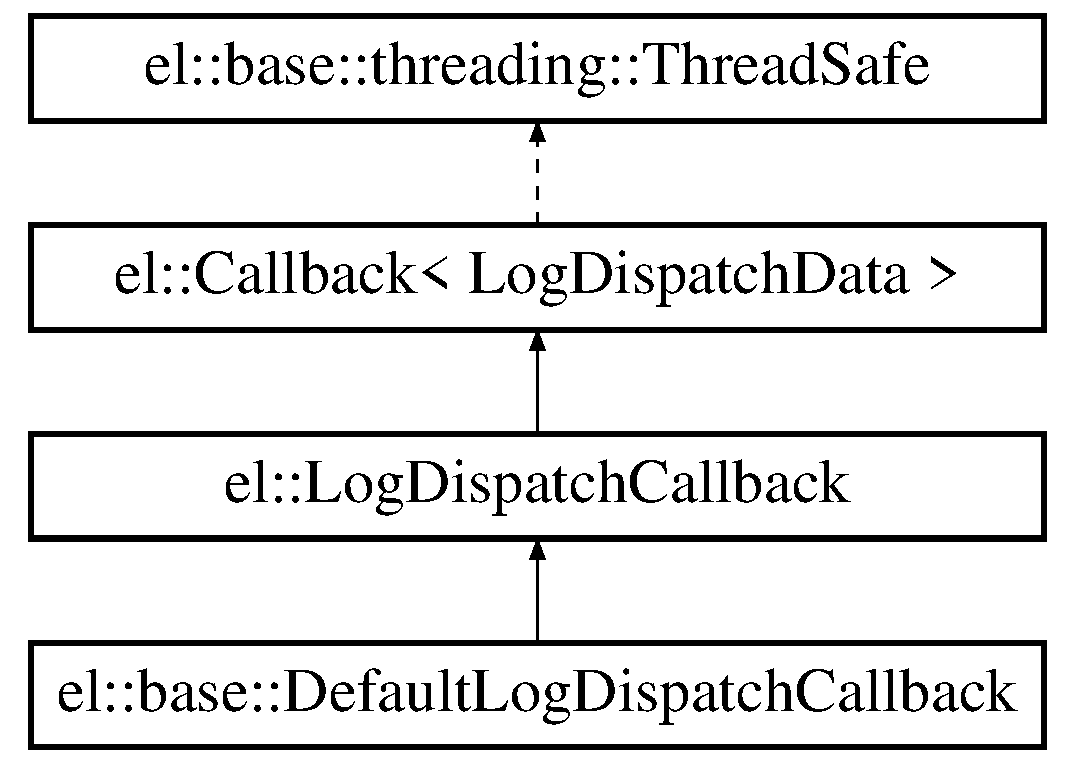
\includegraphics[height=4.000000cm]{classel_1_1base_1_1DefaultLogDispatchCallback}
\end{center}
\end{figure}
\subsection*{Protected Member Functions}
\begin{DoxyCompactItemize}
\item 
\hypertarget{classel_1_1base_1_1DefaultLogDispatchCallback_acdac30f202c245500e6d94c55eee6d95}{void {\bfseries handle} (const \hyperlink{classel_1_1LogDispatchData}{Log\-Dispatch\-Data} $\ast$data)}\label{classel_1_1base_1_1DefaultLogDispatchCallback_acdac30f202c245500e6d94c55eee6d95}

\end{DoxyCompactItemize}
\subsection*{Additional Inherited Members}


The documentation for this class was generated from the following file\-:\begin{DoxyCompactItemize}
\item 
include/sma/io/detail/logimpl.\-hpp\end{DoxyCompactItemize}

\hypertarget{classel_1_1base_1_1DefaultPerformanceTrackingCallback}{\section{el\-:\-:base\-:\-:Default\-Performance\-Tracking\-Callback Class Reference}
\label{classel_1_1base_1_1DefaultPerformanceTrackingCallback}\index{el\-::base\-::\-Default\-Performance\-Tracking\-Callback@{el\-::base\-::\-Default\-Performance\-Tracking\-Callback}}
}
Inheritance diagram for el\-:\-:base\-:\-:Default\-Performance\-Tracking\-Callback\-:\begin{figure}[H]
\begin{center}
\leavevmode
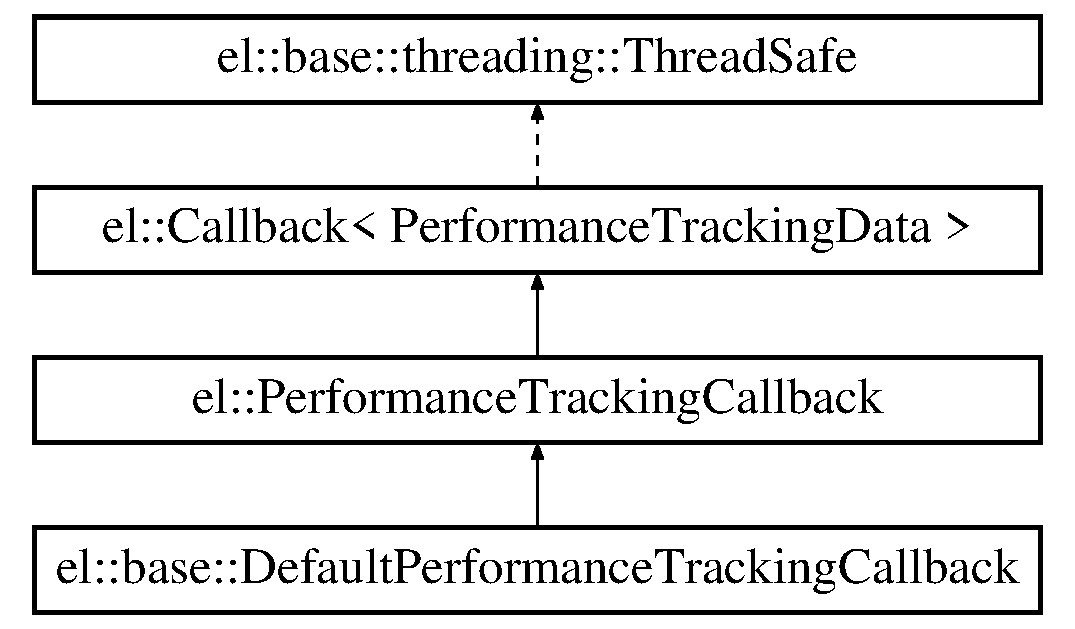
\includegraphics[height=4.000000cm]{classel_1_1base_1_1DefaultPerformanceTrackingCallback}
\end{center}
\end{figure}
\subsection*{Protected Member Functions}
\begin{DoxyCompactItemize}
\item 
\hypertarget{classel_1_1base_1_1DefaultPerformanceTrackingCallback_afabb8820e1bd9a7fb89508fe11f59d37}{void {\bfseries handle} (const \hyperlink{classel_1_1PerformanceTrackingData}{Performance\-Tracking\-Data} $\ast$data)}\label{classel_1_1base_1_1DefaultPerformanceTrackingCallback_afabb8820e1bd9a7fb89508fe11f59d37}

\end{DoxyCompactItemize}
\subsection*{Additional Inherited Members}


The documentation for this class was generated from the following file\-:\begin{DoxyCompactItemize}
\item 
include/sma/io/detail/logimpl.\-hpp\end{DoxyCompactItemize}

\hypertarget{classsma_1_1delay__queue}{\section{sma\-:\-:delay\-\_\-queue$<$ E, Clock $>$ Class Template Reference}
\label{classsma_1_1delay__queue}\index{sma\-::delay\-\_\-queue$<$ E, Clock $>$@{sma\-::delay\-\_\-queue$<$ E, Clock $>$}}
}
\subsection*{Public Member Functions}
\begin{DoxyCompactItemize}
\item 
\hypertarget{classsma_1_1delay__queue_a3f4359c098b76a43374cf19cf3be03db}{{\bfseries delay\-\_\-queue} (const \hyperlink{classsma_1_1delay__queue}{Myt} \&copy)}\label{classsma_1_1delay__queue_a3f4359c098b76a43374cf19cf3be03db}

\item 
\hypertarget{classsma_1_1delay__queue_a112dc1c9ccaef2d7404c6169f2041e89}{{\bfseries delay\-\_\-queue} (\hyperlink{classsma_1_1delay__queue}{Myt} \&\&move)}\label{classsma_1_1delay__queue_a112dc1c9ccaef2d7404c6169f2041e89}

\item 
\hypertarget{classsma_1_1delay__queue_a807d7957eb4beb292b59827aac37f945}{{\footnotesize template$<$typename Delay $>$ }\\void {\bfseries push} (const E \&e, Delay delay)}\label{classsma_1_1delay__queue_a807d7957eb4beb292b59827aac37f945}

\item 
\hypertarget{classsma_1_1delay__queue_abe4f1da5547d72a258562ecb3d2dbc06}{{\footnotesize template$<$typename Delay $>$ }\\void {\bfseries push} (E \&\&e, Delay delay)}\label{classsma_1_1delay__queue_abe4f1da5547d72a258562ecb3d2dbc06}

\item 
\hypertarget{classsma_1_1delay__queue_adb86370b1801fb9ee96028d0af54df89}{E {\bfseries pop} ()}\label{classsma_1_1delay__queue_adb86370b1801fb9ee96028d0af54df89}

\item 
\hypertarget{classsma_1_1delay__queue_acf49578574d2989128eb107616d56a26}{std\-::size\-\_\-t {\bfseries size} ()}\label{classsma_1_1delay__queue_acf49578574d2989128eb107616d56a26}

\item 
\hypertarget{classsma_1_1delay__queue_a0197b8d37227a176bfdd5bc5f8da9489}{bool {\bfseries empty} ()}\label{classsma_1_1delay__queue_a0197b8d37227a176bfdd5bc5f8da9489}

\item 
\hypertarget{classsma_1_1delay__queue_ae634dbb2bc1b6653ca8126d9372cf409}{void {\bfseries interrupt} ()}\label{classsma_1_1delay__queue_ae634dbb2bc1b6653ca8126d9372cf409}

\item 
\hypertarget{classsma_1_1delay__queue_a4459fdf29da74aac8777297bcff28261}{\hyperlink{classsma_1_1delay__queue}{Myt} \& {\bfseries operator=} (const \hyperlink{classsma_1_1delay__queue}{Myt} \&copy)}\label{classsma_1_1delay__queue_a4459fdf29da74aac8777297bcff28261}

\item 
\hypertarget{classsma_1_1delay__queue_a88a2c620324e29e0e448c4d04cb09bbd}{\hyperlink{classsma_1_1delay__queue}{Myt} \& {\bfseries operator=} (\hyperlink{classsma_1_1delay__queue}{Myt} \&\&move)}\label{classsma_1_1delay__queue_a88a2c620324e29e0e448c4d04cb09bbd}

\end{DoxyCompactItemize}


The documentation for this class was generated from the following file\-:\begin{DoxyCompactItemize}
\item 
include/sma/collect/delay\-\_\-queue.\-hpp\end{DoxyCompactItemize}

\hypertarget{classsma_1_1DummyGps}{\section{sma\-:\-:Dummy\-Gps Class Reference}
\label{classsma_1_1DummyGps}\index{sma\-::\-Dummy\-Gps@{sma\-::\-Dummy\-Gps}}
}
Inheritance diagram for sma\-:\-:Dummy\-Gps\-:\begin{figure}[H]
\begin{center}
\leavevmode
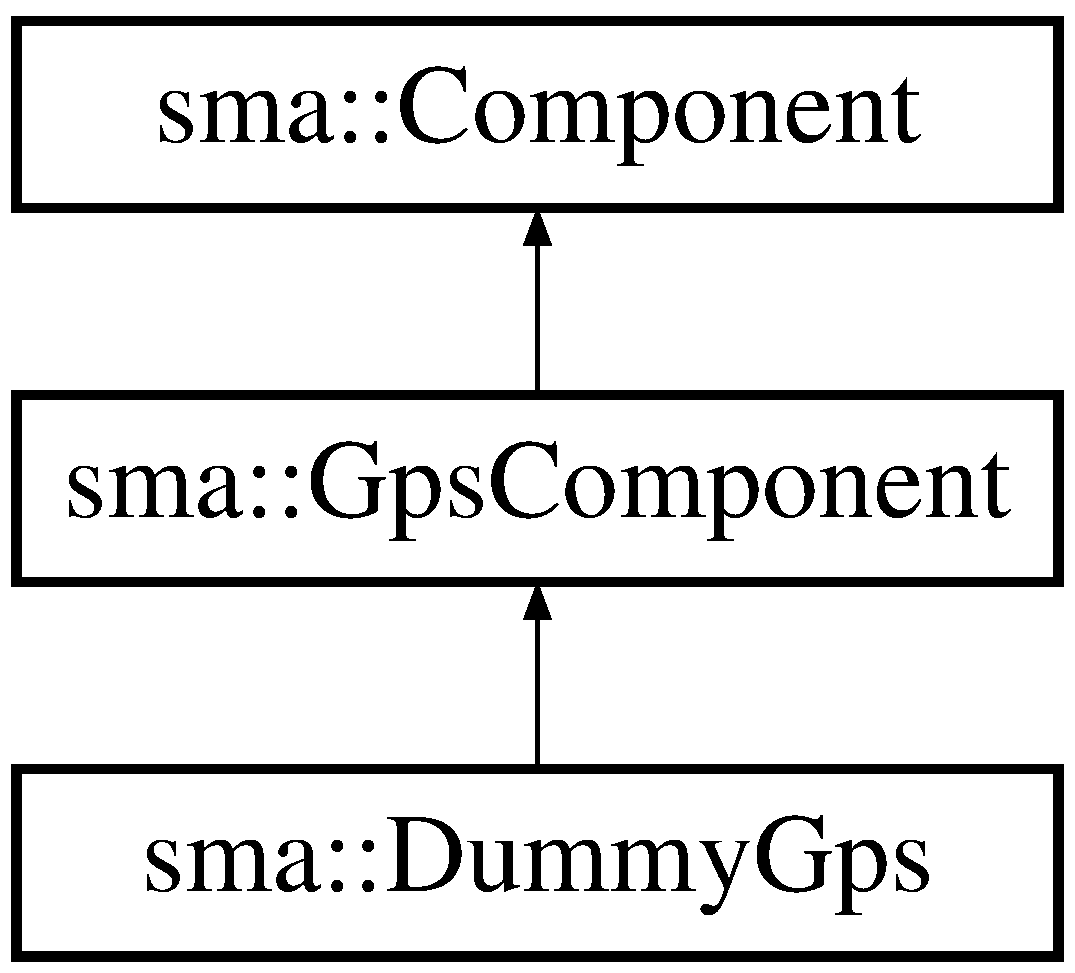
\includegraphics[height=3.000000cm]{classsma_1_1DummyGps}
\end{center}
\end{figure}
\subsection*{Public Member Functions}
\begin{DoxyCompactItemize}
\item 
\hypertarget{classsma_1_1DummyGps_acf3e9fee23aebea4ef1cf6dd3cd142f5}{{\bfseries Dummy\-Gps} (\hyperlink{structsma_1_1GPS_1_1Coord}{G\-P\-S\-::\-Coord} pos)}\label{classsma_1_1DummyGps_acf3e9fee23aebea4ef1cf6dd3cd142f5}

\item 
\hypertarget{classsma_1_1DummyGps_ab18a3ca382c38d9bb4b50b4ff2ff9fd3}{virtual \hyperlink{structsma_1_1GPS_1_1Coord}{G\-P\-S\-::\-Coord} {\bfseries position} () const override}\label{classsma_1_1DummyGps_ab18a3ca382c38d9bb4b50b4ff2ff9fd3}

\end{DoxyCompactItemize}
\subsection*{Protected Attributes}
\begin{DoxyCompactItemize}
\item 
\hypertarget{classsma_1_1DummyGps_a917596110e31f16a4363d3534444f6e9}{\hyperlink{structsma_1_1GPS_1_1Coord}{G\-P\-S\-::\-Coord} {\bfseries pos}}\label{classsma_1_1DummyGps_a917596110e31f16a4363d3534444f6e9}

\end{DoxyCompactItemize}


The documentation for this class was generated from the following file\-:\begin{DoxyCompactItemize}
\item 
include/sma/dummygps.\-hpp\end{DoxyCompactItemize}

\hypertarget{classel_1_1base_1_1utils_1_1File}{\section{el\-:\-:base\-:\-:utils\-:\-:File Class Reference}
\label{classel_1_1base_1_1utils_1_1File}\index{el\-::base\-::utils\-::\-File@{el\-::base\-::utils\-::\-File}}
}
Inheritance diagram for el\-:\-:base\-:\-:utils\-:\-:File\-:\begin{figure}[H]
\begin{center}
\leavevmode
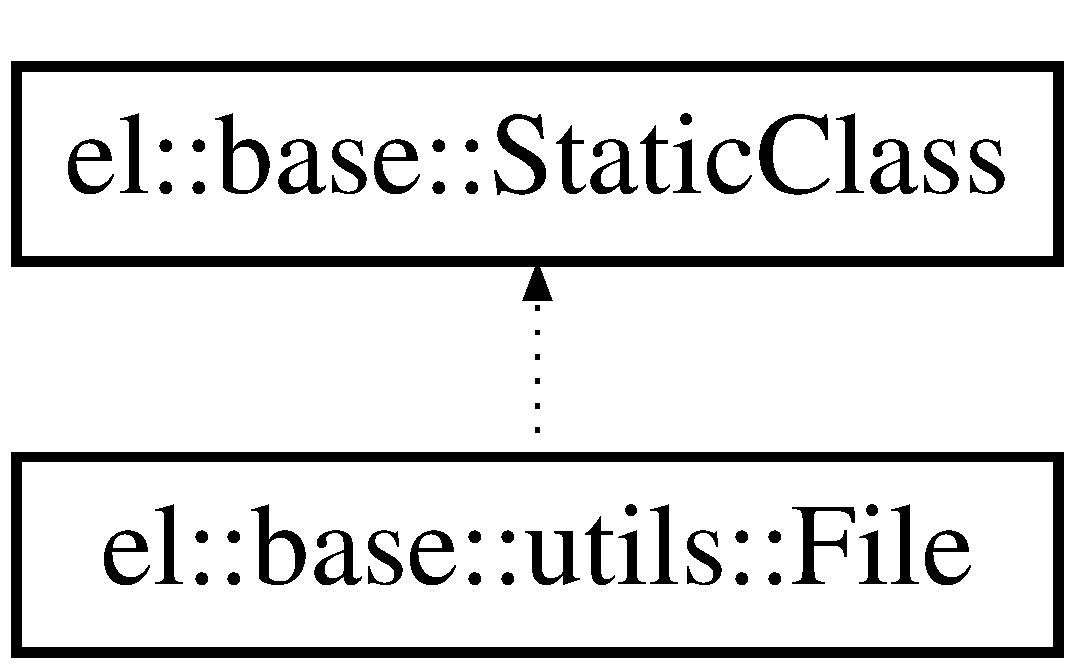
\includegraphics[height=2.000000cm]{classel_1_1base_1_1utils_1_1File}
\end{center}
\end{figure}
\subsection*{Static Public Member Functions}
\begin{DoxyCompactItemize}
\item 
static base\-::type\-::fstream\-\_\-t $\ast$ \hyperlink{classel_1_1base_1_1utils_1_1File_aa4bef1f2e00269d75c1c1eabb0ce4563}{new\-File\-Stream} (const std\-::string \&filename)
\begin{DoxyCompactList}\small\item\em Creates new out file stream for specified filename. \end{DoxyCompactList}\item 
\hypertarget{classel_1_1base_1_1utils_1_1File_a54415ba02f698ba978795265f7f4b86c}{static std\-::size\-\_\-t \hyperlink{classel_1_1base_1_1utils_1_1File_a54415ba02f698ba978795265f7f4b86c}{get\-Size\-Of\-File} (base\-::type\-::fstream\-\_\-t $\ast$fs)}\label{classel_1_1base_1_1utils_1_1File_a54415ba02f698ba978795265f7f4b86c}

\begin{DoxyCompactList}\small\item\em Gets size of file provided in stream. \end{DoxyCompactList}\item 
\hypertarget{classel_1_1base_1_1utils_1_1File_a4fc9e36b814f1aeaa4931e35d58e5b45}{static bool \hyperlink{classel_1_1base_1_1utils_1_1File_a4fc9e36b814f1aeaa4931e35d58e5b45}{path\-Exists} (const char $\ast$path, bool consider\-File=false)}\label{classel_1_1base_1_1utils_1_1File_a4fc9e36b814f1aeaa4931e35d58e5b45}

\begin{DoxyCompactList}\small\item\em Determines whether or not provided path exist in current file system. \end{DoxyCompactList}\item 
static bool \hyperlink{classel_1_1base_1_1utils_1_1File_a34fbb5b06201c7e3db71db80e017fb96}{create\-Path} (const std\-::string \&path)
\begin{DoxyCompactList}\small\item\em Creates specified path on file system. \end{DoxyCompactList}\item 
\hypertarget{classel_1_1base_1_1utils_1_1File_af541c62ed408de7e368d339f96c0c6cf}{static std\-::string \hyperlink{classel_1_1base_1_1utils_1_1File_af541c62ed408de7e368d339f96c0c6cf}{extract\-Path\-From\-Filename} (const std\-::string \&full\-Path, const char $\ast$seperator=base\-::consts\-::k\-File\-Path\-Seperator)}\label{classel_1_1base_1_1utils_1_1File_af541c62ed408de7e368d339f96c0c6cf}

\begin{DoxyCompactList}\small\item\em Extracts path of filename with leading slash. \end{DoxyCompactList}\item 
\hypertarget{classel_1_1base_1_1utils_1_1File_a38e3b3c72f73de47563b289eff13ae2d}{static void \hyperlink{classel_1_1base_1_1utils_1_1File_a38e3b3c72f73de47563b289eff13ae2d}{build\-Stripped\-Filename} (const char $\ast$filename, char buff\mbox{[}$\,$\mbox{]}, std\-::size\-\_\-t limit=base\-::consts\-::k\-Source\-Filename\-Max\-Length)}\label{classel_1_1base_1_1utils_1_1File_a38e3b3c72f73de47563b289eff13ae2d}

\begin{DoxyCompactList}\small\item\em builds stripped filename and puts it in buff \end{DoxyCompactList}\item 
\hypertarget{classel_1_1base_1_1utils_1_1File_ad6c3703c16b95bd4992f501380d503b4}{static void \hyperlink{classel_1_1base_1_1utils_1_1File_ad6c3703c16b95bd4992f501380d503b4}{build\-Base\-Filename} (const std\-::string \&full\-Path, char buff\mbox{[}$\,$\mbox{]}, std\-::size\-\_\-t limit=base\-::consts\-::k\-Source\-Filename\-Max\-Length, const char $\ast$seperator=base\-::consts\-::k\-File\-Path\-Seperator)}\label{classel_1_1base_1_1utils_1_1File_ad6c3703c16b95bd4992f501380d503b4}

\begin{DoxyCompactList}\small\item\em builds base filename and puts it in buff \end{DoxyCompactList}\end{DoxyCompactItemize}


\subsection{Member Function Documentation}
\hypertarget{classel_1_1base_1_1utils_1_1File_a34fbb5b06201c7e3db71db80e017fb96}{\index{el\-::base\-::utils\-::\-File@{el\-::base\-::utils\-::\-File}!create\-Path@{create\-Path}}
\index{create\-Path@{create\-Path}!el::base::utils::File@{el\-::base\-::utils\-::\-File}}
\subsubsection[{create\-Path}]{\setlength{\rightskip}{0pt plus 5cm}static bool el\-::base\-::utils\-::\-File\-::create\-Path (
\begin{DoxyParamCaption}
\item[{const std\-::string \&}]{path}
\end{DoxyParamCaption}
)\hspace{0.3cm}{\ttfamily [inline]}, {\ttfamily [static]}}}\label{classel_1_1base_1_1utils_1_1File_a34fbb5b06201c7e3db71db80e017fb96}


Creates specified path on file system. 


\begin{DoxyParams}{Parameters}
{\em path} & Path to create. \\
\hline
\end{DoxyParams}
\hypertarget{classel_1_1base_1_1utils_1_1File_aa4bef1f2e00269d75c1c1eabb0ce4563}{\index{el\-::base\-::utils\-::\-File@{el\-::base\-::utils\-::\-File}!new\-File\-Stream@{new\-File\-Stream}}
\index{new\-File\-Stream@{new\-File\-Stream}!el::base::utils::File@{el\-::base\-::utils\-::\-File}}
\subsubsection[{new\-File\-Stream}]{\setlength{\rightskip}{0pt plus 5cm}static base\-::type\-::fstream\-\_\-t$\ast$ el\-::base\-::utils\-::\-File\-::new\-File\-Stream (
\begin{DoxyParamCaption}
\item[{const std\-::string \&}]{filename}
\end{DoxyParamCaption}
)\hspace{0.3cm}{\ttfamily [inline]}, {\ttfamily [static]}}}\label{classel_1_1base_1_1utils_1_1File_aa4bef1f2e00269d75c1c1eabb0ce4563}


Creates new out file stream for specified filename. 

\begin{DoxyReturn}{Returns}
Pointer to newly created fstream or nullptr 
\end{DoxyReturn}


The documentation for this class was generated from the following file\-:\begin{DoxyCompactItemize}
\item 
include/sma/io/detail/logimpl.\-hpp\end{DoxyCompactItemize}

\hypertarget{classsma_1_1ForwardStrategy}{\section{sma\-:\-:Forward\-Strategy Class Reference}
\label{classsma_1_1ForwardStrategy}\index{sma\-::\-Forward\-Strategy@{sma\-::\-Forward\-Strategy}}
}
Inheritance diagram for sma\-:\-:Forward\-Strategy\-:\begin{figure}[H]
\begin{center}
\leavevmode
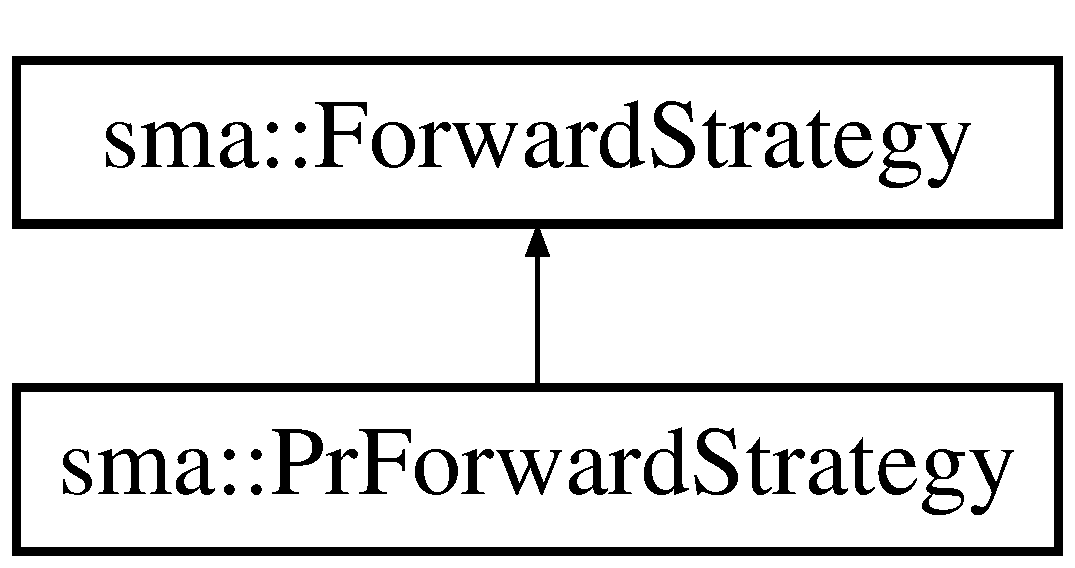
\includegraphics[height=2.000000cm]{classsma_1_1ForwardStrategy}
\end{center}
\end{figure}
\subsection*{Public Member Functions}
\begin{DoxyCompactItemize}
\item 
\hypertarget{classsma_1_1ForwardStrategy_a1fcfe45c9151af87d9c89b27bc3bd6f5}{{\bfseries Forward\-Strategy} (\hyperlink{classsma_1_1LinkLayer}{Link\-Layer} \&llayer)}\label{classsma_1_1ForwardStrategy_a1fcfe45c9151af87d9c89b27bc3bd6f5}

\item 
\hypertarget{classsma_1_1ForwardStrategy_a0a3f2d1ae1e3a845d9d563bbd4eba1f4}{virtual void {\bfseries notify} ()=0}\label{classsma_1_1ForwardStrategy_a0a3f2d1ae1e3a845d9d563bbd4eba1f4}

\end{DoxyCompactItemize}
\subsection*{Protected Attributes}
\begin{DoxyCompactItemize}
\item 
\hypertarget{classsma_1_1ForwardStrategy_a8e701f86c4fd501d0a4ba42566247c1d}{\hyperlink{classsma_1_1LinkLayer}{Link\-Layer} $\ast$ {\bfseries llayer}}\label{classsma_1_1ForwardStrategy_a8e701f86c4fd501d0a4ba42566247c1d}

\end{DoxyCompactItemize}


The documentation for this class was generated from the following files\-:\begin{DoxyCompactItemize}
\item 
include/sma/forwardstrategy.\-hpp\item 
src/forwardstrategy.\-cpp\end{DoxyCompactItemize}

\hypertarget{classsma_1_1GPS}{\section{sma\-:\-:G\-P\-S Class Reference}
\label{classsma_1_1GPS}\index{sma\-::\-G\-P\-S@{sma\-::\-G\-P\-S}}
}
\subsection*{Classes}
\begin{DoxyCompactItemize}
\item 
struct \hyperlink{structsma_1_1GPS_1_1Coord}{Coord}
\end{DoxyCompactItemize}


The documentation for this class was generated from the following file\-:\begin{DoxyCompactItemize}
\item 
include/sma/gps.\-hpp\end{DoxyCompactItemize}

\hypertarget{classsma_1_1GpsComponent}{\section{sma\-:\-:Gps\-Component Class Reference}
\label{classsma_1_1GpsComponent}\index{sma\-::\-Gps\-Component@{sma\-::\-Gps\-Component}}
}
Inheritance diagram for sma\-:\-:Gps\-Component\-:\begin{figure}[H]
\begin{center}
\leavevmode
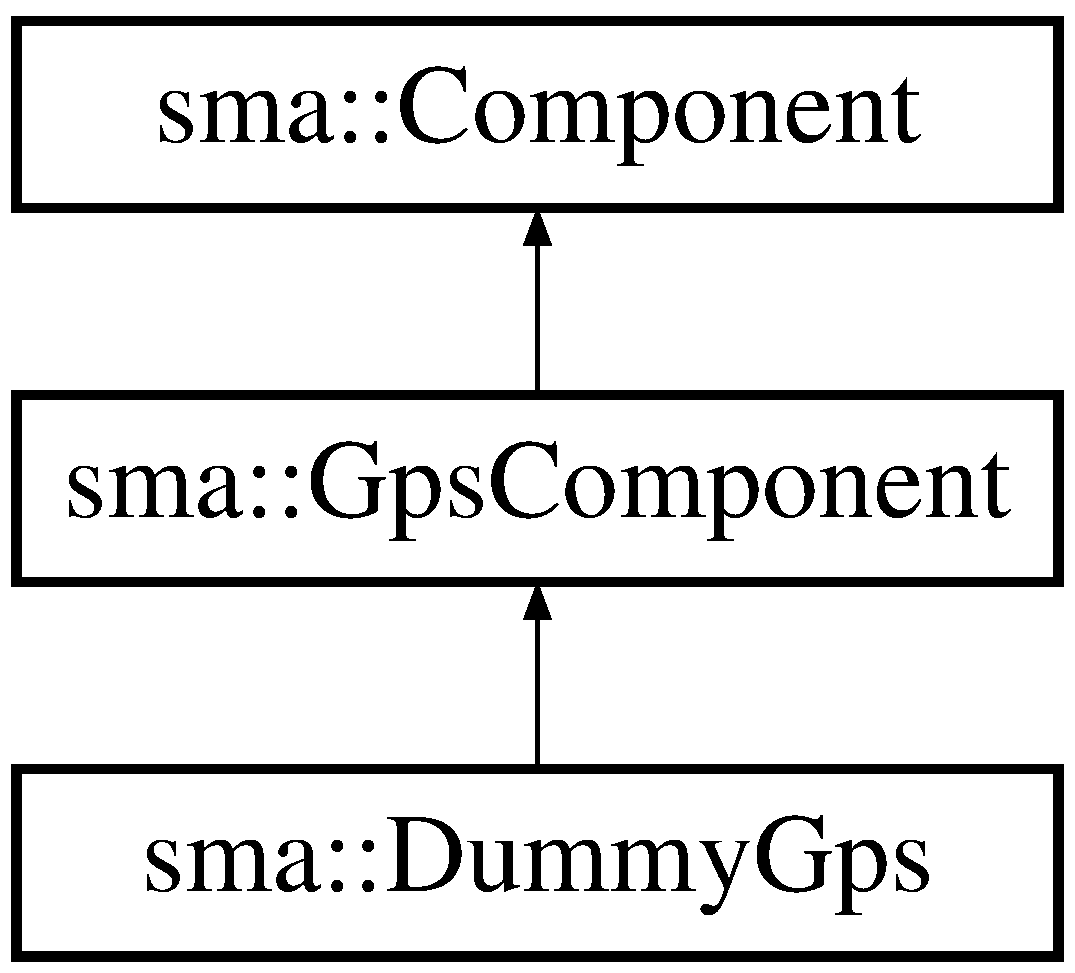
\includegraphics[height=3.000000cm]{classsma_1_1GpsComponent}
\end{center}
\end{figure}
\subsection*{Public Member Functions}
\begin{DoxyCompactItemize}
\item 
\hypertarget{classsma_1_1GpsComponent_a009d95eced02ca9c686998af87a8a570}{virtual \hyperlink{structsma_1_1GPS_1_1Coord}{G\-P\-S\-::\-Coord} {\bfseries position} () const =0}\label{classsma_1_1GpsComponent_a009d95eced02ca9c686998af87a8a570}

\end{DoxyCompactItemize}


The documentation for this class was generated from the following file\-:\begin{DoxyCompactItemize}
\item 
include/sma/gpscomponent.\-hpp\end{DoxyCompactItemize}

\hypertarget{structsma_1_1Hash}{\section{sma\-:\-:Hash Struct Reference}
\label{structsma_1_1Hash}\index{sma\-::\-Hash@{sma\-::\-Hash}}
}
\subsection*{Public Member Functions}
\begin{DoxyCompactItemize}
\item 
\hypertarget{structsma_1_1Hash_a66d153bdafd406376aa07b61feed174b}{{\bfseries Hash} (\hyperlink{structsma_1_1Hash}{Hash} const \&)}\label{structsma_1_1Hash_a66d153bdafd406376aa07b61feed174b}

\item 
\hypertarget{structsma_1_1Hash_ab54e4d5010fc1ce9e1aae01eff0862c6}{\hyperlink{structsma_1_1Hash}{Hash} \& {\bfseries operator=} (\hyperlink{structsma_1_1Hash}{Hash} const \&)}\label{structsma_1_1Hash_ab54e4d5010fc1ce9e1aae01eff0862c6}

\item 
\hypertarget{structsma_1_1Hash_a1debd47ad54c7c4df533c60cac58b182}{{\bfseries D\-E\-S\-E\-R\-I\-A\-L\-I\-Z\-I\-N\-G\-\_\-\-C\-T\-O\-R} (\hyperlink{structsma_1_1Hash}{Hash})}\label{structsma_1_1Hash_a1debd47ad54c7c4df533c60cac58b182}

\item 
\hypertarget{structsma_1_1Hash_a99b7f90e7b4a317f9bf6a492c03340d2}{{\bfseries S\-E\-R\-I\-A\-L\-I\-Z\-E\-R} ()}\label{structsma_1_1Hash_a99b7f90e7b4a317f9bf6a492c03340d2}

\item 
\hypertarget{structsma_1_1Hash_a608333bbc7e8f3f37c2ed49d1ef72237}{int {\bfseries compare} (\hyperlink{structsma_1_1Hash}{Hash} const \&) const }\label{structsma_1_1Hash_a608333bbc7e8f3f37c2ed49d1ef72237}

\item 
\hypertarget{structsma_1_1Hash_a99082a7a7915e01ec4a3d858e5db2cb8}{bool {\bfseries operator==} (\hyperlink{structsma_1_1Hash}{Hash} const \&r) const }\label{structsma_1_1Hash_a99082a7a7915e01ec4a3d858e5db2cb8}

\item 
\hypertarget{structsma_1_1Hash_abeace2f93af8d81eb0afb1a6d43e88b1}{bool {\bfseries operator!=} (\hyperlink{structsma_1_1Hash}{Hash} const \&r) const }\label{structsma_1_1Hash_abeace2f93af8d81eb0afb1a6d43e88b1}

\item 
\hypertarget{structsma_1_1Hash_aa811d9fb7dedacd1c4fb6942208f3b10}{bool {\bfseries operator$<$} (\hyperlink{structsma_1_1Hash}{Hash} const \&r) const }\label{structsma_1_1Hash_aa811d9fb7dedacd1c4fb6942208f3b10}

\item 
\hypertarget{structsma_1_1Hash_a15198c79f588abde88bb159708a4cab9}{bool {\bfseries operator$>$} (\hyperlink{structsma_1_1Hash}{Hash} const \&r) const }\label{structsma_1_1Hash_a15198c79f588abde88bb159708a4cab9}

\item 
\hypertarget{structsma_1_1Hash_a2d0c5d092d0007f0a6391559f0a5f722}{bool {\bfseries operator$<$=} (\hyperlink{structsma_1_1Hash}{Hash} const \&r) const }\label{structsma_1_1Hash_a2d0c5d092d0007f0a6391559f0a5f722}

\item 
\hypertarget{structsma_1_1Hash_a7c7a9f933dd3af05335a70a09a53a897}{bool {\bfseries operator$>$=} (\hyperlink{structsma_1_1Hash}{Hash} const \&r) const }\label{structsma_1_1Hash_a7c7a9f933dd3af05335a70a09a53a897}

\item 
\hypertarget{structsma_1_1Hash_a68bbcc1f267c5dc78a7f7005a84d2d1d}{{\bfseries operator std\-::string} () const }\label{structsma_1_1Hash_a68bbcc1f267c5dc78a7f7005a84d2d1d}

\end{DoxyCompactItemize}
\subsection*{Static Public Attributes}
\begin{DoxyCompactItemize}
\item 
\hypertarget{structsma_1_1Hash_a70604fa3eae1c821132295268dc62aef}{static constexpr std\-::size\-\_\-t {\bfseries L\-E\-N\-G\-T\-H} = 32}\label{structsma_1_1Hash_a70604fa3eae1c821132295268dc62aef}

\end{DoxyCompactItemize}
\subsection*{Friends}
\begin{DoxyCompactItemize}
\item 
\hypertarget{structsma_1_1Hash_a50630f6cacf6bbaf65b18c54ef72b343}{struct {\bfseries Hasher}}\label{structsma_1_1Hash_a50630f6cacf6bbaf65b18c54ef72b343}

\item 
\hypertarget{structsma_1_1Hash_a5f6403cd6c7fa0207cf3093a6c1a166f}{struct {\bfseries std\-::hash$<$ Hash $>$}}\label{structsma_1_1Hash_a5f6403cd6c7fa0207cf3093a6c1a166f}

\end{DoxyCompactItemize}


The documentation for this struct was generated from the following files\-:\begin{DoxyCompactItemize}
\item 
include/sma/util/hash.\-hpp\item 
src/util/hash.\-cpp\end{DoxyCompactItemize}

\hypertarget{structstd_1_1hash_3_01ns3_1_1EventId_01_4}{\section{std\-:\-:hash$<$ ns3\-:\-:Event\-Id $>$ Struct Template Reference}
\label{structstd_1_1hash_3_01ns3_1_1EventId_01_4}\index{std\-::hash$<$ ns3\-::\-Event\-Id $>$@{std\-::hash$<$ ns3\-::\-Event\-Id $>$}}
}
\subsection*{Public Types}
\begin{DoxyCompactItemize}
\item 
\hypertarget{structstd_1_1hash_3_01ns3_1_1EventId_01_4_a2c48c6c1f4ea8b1710f858c53c4e1b98}{using {\bfseries argument\-\_\-type} = ns3\-::\-Event\-Id}\label{structstd_1_1hash_3_01ns3_1_1EventId_01_4_a2c48c6c1f4ea8b1710f858c53c4e1b98}

\item 
\hypertarget{structstd_1_1hash_3_01ns3_1_1EventId_01_4_a471ca48ea3bae2a14521817255409f95}{using {\bfseries result\-\_\-type} = std\-::size\-\_\-t}\label{structstd_1_1hash_3_01ns3_1_1EventId_01_4_a471ca48ea3bae2a14521817255409f95}

\end{DoxyCompactItemize}
\subsection*{Public Member Functions}
\begin{DoxyCompactItemize}
\item 
\hypertarget{structstd_1_1hash_3_01ns3_1_1EventId_01_4_a031f6a21ea07a32477fe42ca6b2c7244}{result\-\_\-type {\bfseries operator()} (argument\-\_\-type const \&a) const }\label{structstd_1_1hash_3_01ns3_1_1EventId_01_4_a031f6a21ea07a32477fe42ca6b2c7244}

\end{DoxyCompactItemize}


The documentation for this struct was generated from the following file\-:\begin{DoxyCompactItemize}
\item 
ns3/src/async.\-cpp\end{DoxyCompactItemize}

\hypertarget{structstd_1_1hash_3_01sma_1_1ContentDescriptor_01_4}{\section{std\-:\-:hash$<$ sma\-:\-:Content\-Descriptor $>$ Struct Template Reference}
\label{structstd_1_1hash_3_01sma_1_1ContentDescriptor_01_4}\index{std\-::hash$<$ sma\-::\-Content\-Descriptor $>$@{std\-::hash$<$ sma\-::\-Content\-Descriptor $>$}}
}
\subsection*{Public Types}
\begin{DoxyCompactItemize}
\item 
\hypertarget{structstd_1_1hash_3_01sma_1_1ContentDescriptor_01_4_ac4bb043ede97817f9d8b79ab54a60fdc}{using {\bfseries argument\-\_\-type} = \hyperlink{structsma_1_1ContentDescriptor}{sma\-::\-Content\-Descriptor}}\label{structstd_1_1hash_3_01sma_1_1ContentDescriptor_01_4_ac4bb043ede97817f9d8b79ab54a60fdc}

\item 
\hypertarget{structstd_1_1hash_3_01sma_1_1ContentDescriptor_01_4_a11c2c83e5219f970274b9e409ad72a8f}{using {\bfseries result\-\_\-type} = size\-\_\-t}\label{structstd_1_1hash_3_01sma_1_1ContentDescriptor_01_4_a11c2c83e5219f970274b9e409ad72a8f}

\end{DoxyCompactItemize}
\subsection*{Public Member Functions}
\begin{DoxyCompactItemize}
\item 
\hypertarget{structstd_1_1hash_3_01sma_1_1ContentDescriptor_01_4_aa65743dc59a0ebd581e118c7768e7b4b}{result\-\_\-type {\bfseries operator()} (\hyperlink{structsma_1_1ContentDescriptor}{argument\-\_\-type} const \&info) const }\label{structstd_1_1hash_3_01sma_1_1ContentDescriptor_01_4_aa65743dc59a0ebd581e118c7768e7b4b}

\end{DoxyCompactItemize}


The documentation for this struct was generated from the following file\-:\begin{DoxyCompactItemize}
\item 
include/sma/ccn/contentdescriptor.\-hpp\end{DoxyCompactItemize}

\hypertarget{structstd_1_1hash_3_01sma_1_1ContentName_01_4}{\section{std\-:\-:hash$<$ sma\-:\-:Content\-Name $>$ Struct Template Reference}
\label{structstd_1_1hash_3_01sma_1_1ContentName_01_4}\index{std\-::hash$<$ sma\-::\-Content\-Name $>$@{std\-::hash$<$ sma\-::\-Content\-Name $>$}}
}
\subsection*{Public Types}
\begin{DoxyCompactItemize}
\item 
\hypertarget{structstd_1_1hash_3_01sma_1_1ContentName_01_4_a7092be18c3d9018045a00e06d249f9c5}{using {\bfseries argument\-\_\-type} = \hyperlink{structsma_1_1ContentName}{sma\-::\-Content\-Name}}\label{structstd_1_1hash_3_01sma_1_1ContentName_01_4_a7092be18c3d9018045a00e06d249f9c5}

\item 
\hypertarget{structstd_1_1hash_3_01sma_1_1ContentName_01_4_a2a85a37789944d25c03743dc6f306acd}{using {\bfseries result\-\_\-type} = std\-::size\-\_\-t}\label{structstd_1_1hash_3_01sma_1_1ContentName_01_4_a2a85a37789944d25c03743dc6f306acd}

\end{DoxyCompactItemize}
\subsection*{Public Member Functions}
\begin{DoxyCompactItemize}
\item 
\hypertarget{structstd_1_1hash_3_01sma_1_1ContentName_01_4_aa87628bfbf5ca3191e3f9f01818f9046}{result\-\_\-type {\bfseries operator()} (\hyperlink{structsma_1_1ContentName}{argument\-\_\-type} const \&a) const }\label{structstd_1_1hash_3_01sma_1_1ContentName_01_4_aa87628bfbf5ca3191e3f9f01818f9046}

\end{DoxyCompactItemize}


The documentation for this struct was generated from the following file\-:\begin{DoxyCompactItemize}
\item 
include/sma/ccn/contentname.\-hpp\end{DoxyCompactItemize}

\hypertarget{structstd_1_1hash_3_01sma_1_1ContentType_01_4}{\section{std\-:\-:hash$<$ sma\-:\-:Content\-Type $>$ Struct Template Reference}
\label{structstd_1_1hash_3_01sma_1_1ContentType_01_4}\index{std\-::hash$<$ sma\-::\-Content\-Type $>$@{std\-::hash$<$ sma\-::\-Content\-Type $>$}}
}
\subsection*{Public Types}
\begin{DoxyCompactItemize}
\item 
\hypertarget{structstd_1_1hash_3_01sma_1_1ContentType_01_4_aa6f30018c2283fec5c14d3bded616b05}{using {\bfseries argument\-\_\-type} = \hyperlink{structsma_1_1ContentType}{sma\-::\-Content\-Type}}\label{structstd_1_1hash_3_01sma_1_1ContentType_01_4_aa6f30018c2283fec5c14d3bded616b05}

\item 
\hypertarget{structstd_1_1hash_3_01sma_1_1ContentType_01_4_a48c332fb1e0d1a96ee083d9e77f77e97}{using {\bfseries result\-\_\-type} = std\-::size\-\_\-t}\label{structstd_1_1hash_3_01sma_1_1ContentType_01_4_a48c332fb1e0d1a96ee083d9e77f77e97}

\end{DoxyCompactItemize}
\subsection*{Public Member Functions}
\begin{DoxyCompactItemize}
\item 
\hypertarget{structstd_1_1hash_3_01sma_1_1ContentType_01_4_a8c72d9477b7fb948ef782ecd7ee86fb6}{result\-\_\-type {\bfseries operator()} (\hyperlink{structsma_1_1ContentType}{argument\-\_\-type} const \&a) const }\label{structstd_1_1hash_3_01sma_1_1ContentType_01_4_a8c72d9477b7fb948ef782ecd7ee86fb6}

\end{DoxyCompactItemize}


The documentation for this struct was generated from the following file\-:\begin{DoxyCompactItemize}
\item 
include/sma/ccn/contenttype.\-hpp\end{DoxyCompactItemize}

\hypertarget{structstd_1_1hash_3_01sma_1_1Hash_01_4}{\section{std\-:\-:hash$<$ sma\-:\-:Hash $>$ Struct Template Reference}
\label{structstd_1_1hash_3_01sma_1_1Hash_01_4}\index{std\-::hash$<$ sma\-::\-Hash $>$@{std\-::hash$<$ sma\-::\-Hash $>$}}
}
\subsection*{Public Types}
\begin{DoxyCompactItemize}
\item 
\hypertarget{structstd_1_1hash_3_01sma_1_1Hash_01_4_ac19ac5fa9d7134e6cae9b75a2b3f4c73}{using {\bfseries argument\-\_\-type} = \hyperlink{structsma_1_1Hash}{sma\-::\-Hash}}\label{structstd_1_1hash_3_01sma_1_1Hash_01_4_ac19ac5fa9d7134e6cae9b75a2b3f4c73}

\item 
\hypertarget{structstd_1_1hash_3_01sma_1_1Hash_01_4_aec7fbba93db28c8c3f833b4042f109b3}{using {\bfseries result\-\_\-type} = size\-\_\-t}\label{structstd_1_1hash_3_01sma_1_1Hash_01_4_aec7fbba93db28c8c3f833b4042f109b3}

\end{DoxyCompactItemize}
\subsection*{Public Member Functions}
\begin{DoxyCompactItemize}
\item 
\hypertarget{structstd_1_1hash_3_01sma_1_1Hash_01_4_a87f796dbb840c3f99fcae9548962406f}{result\-\_\-type {\bfseries operator()} (\hyperlink{structsma_1_1Hash}{argument\-\_\-type} const \&a) const }\label{structstd_1_1hash_3_01sma_1_1Hash_01_4_a87f796dbb840c3f99fcae9548962406f}

\end{DoxyCompactItemize}


The documentation for this struct was generated from the following file\-:\begin{DoxyCompactItemize}
\item 
include/sma/util/hash.\-hpp\end{DoxyCompactItemize}

\hypertarget{structstd_1_1hash_3_01sma_1_1InterestRank_01_4}{\section{std\-:\-:hash$<$ sma\-:\-:Interest\-Rank $>$ Struct Template Reference}
\label{structstd_1_1hash_3_01sma_1_1InterestRank_01_4}\index{std\-::hash$<$ sma\-::\-Interest\-Rank $>$@{std\-::hash$<$ sma\-::\-Interest\-Rank $>$}}
}
\subsection*{Public Types}
\begin{DoxyCompactItemize}
\item 
\hypertarget{structstd_1_1hash_3_01sma_1_1InterestRank_01_4_ad3b0657fad0aed6f46192ee5389e6644}{using {\bfseries argument\-\_\-type} = \hyperlink{structsma_1_1InterestRank}{sma\-::\-Interest\-Rank}}\label{structstd_1_1hash_3_01sma_1_1InterestRank_01_4_ad3b0657fad0aed6f46192ee5389e6644}

\item 
\hypertarget{structstd_1_1hash_3_01sma_1_1InterestRank_01_4_adfc72e7f6e7ac0bfb0ea5eecd132b027}{using {\bfseries result\-\_\-type} = std\-::size\-\_\-t}\label{structstd_1_1hash_3_01sma_1_1InterestRank_01_4_adfc72e7f6e7ac0bfb0ea5eecd132b027}

\end{DoxyCompactItemize}
\subsection*{Public Member Functions}
\begin{DoxyCompactItemize}
\item 
\hypertarget{structstd_1_1hash_3_01sma_1_1InterestRank_01_4_a07924b0cd58aa820678a516aaaa4efdc}{result\-\_\-type {\bfseries operator()} (\hyperlink{structsma_1_1InterestRank}{argument\-\_\-type} const \&a) const }\label{structstd_1_1hash_3_01sma_1_1InterestRank_01_4_a07924b0cd58aa820678a516aaaa4efdc}

\end{DoxyCompactItemize}


The documentation for this struct was generated from the following file\-:\begin{DoxyCompactItemize}
\item 
include/sma/ccn/interestrank.\-hpp\end{DoxyCompactItemize}

\hypertarget{structstd_1_1hash_3_01sma_1_1NodeId_01_4}{\section{std\-:\-:hash$<$ sma\-:\-:Node\-Id $>$ Struct Template Reference}
\label{structstd_1_1hash_3_01sma_1_1NodeId_01_4}\index{std\-::hash$<$ sma\-::\-Node\-Id $>$@{std\-::hash$<$ sma\-::\-Node\-Id $>$}}
}
\subsection*{Public Types}
\begin{DoxyCompactItemize}
\item 
\hypertarget{structstd_1_1hash_3_01sma_1_1NodeId_01_4_a5849f5c115a984c18ee9602524c83ba7}{using {\bfseries argument\-\_\-type} = \hyperlink{structsma_1_1NodeId}{sma\-::\-Node\-Id}}\label{structstd_1_1hash_3_01sma_1_1NodeId_01_4_a5849f5c115a984c18ee9602524c83ba7}

\item 
\hypertarget{structstd_1_1hash_3_01sma_1_1NodeId_01_4_a5cd146b670357fec00967b84286ae41c}{using {\bfseries result\-\_\-type} = std\-::size\-\_\-t}\label{structstd_1_1hash_3_01sma_1_1NodeId_01_4_a5cd146b670357fec00967b84286ae41c}

\end{DoxyCompactItemize}
\subsection*{Public Member Functions}
\begin{DoxyCompactItemize}
\item 
\hypertarget{structstd_1_1hash_3_01sma_1_1NodeId_01_4_a1a2bcc384669e25f2886fdddcf75c77c}{result\-\_\-type {\bfseries operator()} (\hyperlink{structsma_1_1NodeId}{argument\-\_\-type} const \&a) const }\label{structstd_1_1hash_3_01sma_1_1NodeId_01_4_a1a2bcc384669e25f2886fdddcf75c77c}

\end{DoxyCompactItemize}


The documentation for this struct was generated from the following file\-:\begin{DoxyCompactItemize}
\item 
include/sma/nodeid.\-hpp\end{DoxyCompactItemize}

\hypertarget{structsma_1_1Hasher}{\section{sma\-:\-:Hasher Struct Reference}
\label{structsma_1_1Hasher}\index{sma\-::\-Hasher@{sma\-::\-Hasher}}
}
\subsection*{Public Member Functions}
\begin{DoxyCompactItemize}
\item 
\hypertarget{structsma_1_1Hasher_a67c7aadbafb52da2108eaba9a96a7a76}{{\bfseries Hasher} (void const $\ast$src, std\-::size\-\_\-t size)}\label{structsma_1_1Hasher_a67c7aadbafb52da2108eaba9a96a7a76}

\item 
\hypertarget{structsma_1_1Hasher_af45ac064b0f630f261734a08746b352c}{{\bfseries Hasher} (std\-::string const \&s)}\label{structsma_1_1Hasher_af45ac064b0f630f261734a08746b352c}

\item 
\hypertarget{structsma_1_1Hasher_a4eb29e4bc3bc23beca94d24193911068}{\hyperlink{structsma_1_1Hasher}{Hasher} \& {\bfseries operator()} (void const $\ast$src, std\-::size\-\_\-t size)}\label{structsma_1_1Hasher_a4eb29e4bc3bc23beca94d24193911068}

\item 
\hypertarget{structsma_1_1Hasher_af548182cff6ccaed07bc3a6fe33e4c14}{\hyperlink{structsma_1_1Hasher}{Hasher} \& {\bfseries operator()} (std\-::string const \&s)}\label{structsma_1_1Hasher_af548182cff6ccaed07bc3a6fe33e4c14}

\item 
\hypertarget{structsma_1_1Hasher_ae2b0b4ba4202709e6e37148aef92c420}{\hyperlink{structsma_1_1Hash}{Hash} {\bfseries digest} ()}\label{structsma_1_1Hasher_ae2b0b4ba4202709e6e37148aef92c420}

\end{DoxyCompactItemize}


The documentation for this struct was generated from the following files\-:\begin{DoxyCompactItemize}
\item 
include/sma/util/hash.\-hpp\item 
src/util/hash.\-cpp\end{DoxyCompactItemize}

\hypertarget{classsma_1_1Helper}{\section{sma\-:\-:Helper Class Reference}
\label{classsma_1_1Helper}\index{sma\-::\-Helper@{sma\-::\-Helper}}
}
Inheritance diagram for sma\-:\-:Helper\-:\begin{figure}[H]
\begin{center}
\leavevmode
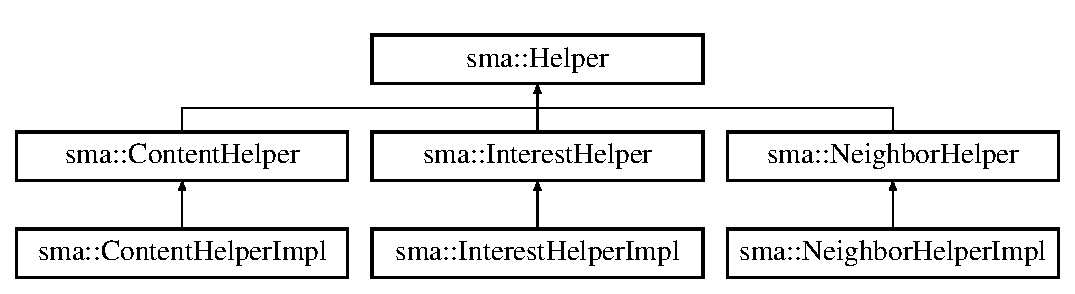
\includegraphics[height=3.000000cm]{classsma_1_1Helper}
\end{center}
\end{figure}
\subsection*{Public Member Functions}
\begin{DoxyCompactItemize}
\item 
\hypertarget{classsma_1_1Helper_ad7183fc108e95cea361bd1637aaef450}{{\bfseries Helper} (\hyperlink{classsma_1_1CcnNode}{Ccn\-Node} \&node)}\label{classsma_1_1Helper_ad7183fc108e95cea361bd1637aaef450}

\end{DoxyCompactItemize}
\subsection*{Protected Attributes}
\begin{DoxyCompactItemize}
\item 
\hypertarget{classsma_1_1Helper_a8a414c1a1e79e1665edc2abedcee6e38}{\hyperlink{classsma_1_1CcnNode}{Ccn\-Node} $\ast$ {\bfseries node}}\label{classsma_1_1Helper_a8a414c1a1e79e1665edc2abedcee6e38}

\item 
\hypertarget{classsma_1_1Helper_a154d33475a59fb49fcad4ba2288d7ef9}{\hyperlink{structsma_1_1Logger}{Logger} {\bfseries log}}\label{classsma_1_1Helper_a154d33475a59fb49fcad4ba2288d7ef9}

\end{DoxyCompactItemize}


The documentation for this class was generated from the following files\-:\begin{DoxyCompactItemize}
\item 
include/sma/helper.\-hpp\item 
src/helper.\-cpp\end{DoxyCompactItemize}

\hypertarget{classel_1_1Helpers}{\section{el\-:\-:Helpers Class Reference}
\label{classel_1_1Helpers}\index{el\-::\-Helpers@{el\-::\-Helpers}}
}


Static helpers for developers.  




{\ttfamily \#include $<$logimpl.\-hpp$>$}

Inheritance diagram for el\-:\-:Helpers\-:\begin{figure}[H]
\begin{center}
\leavevmode
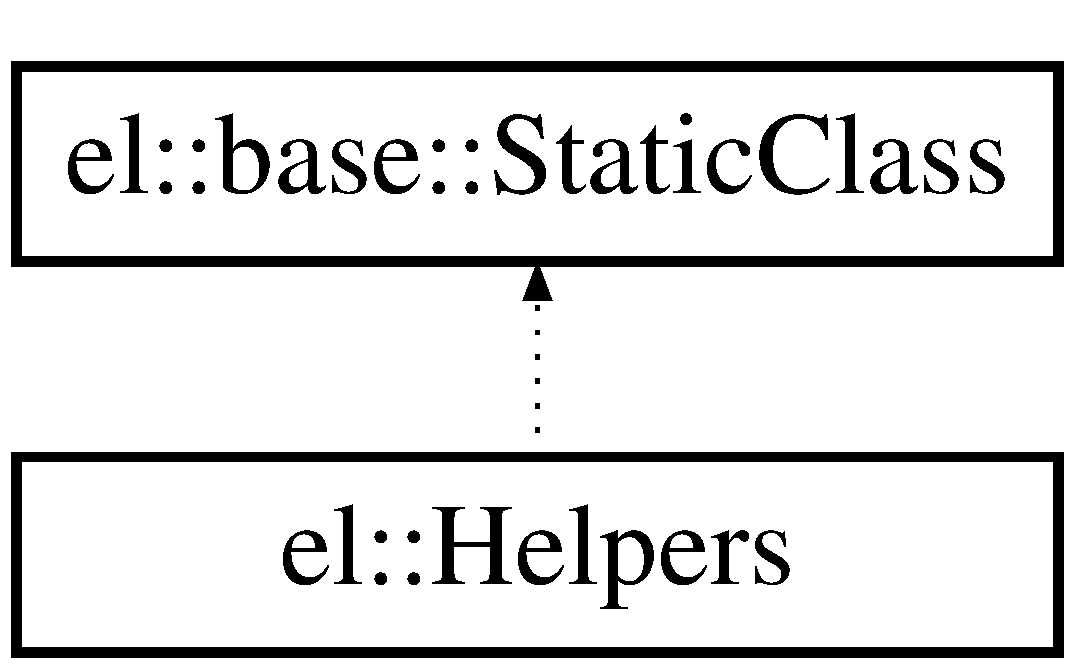
\includegraphics[height=2.000000cm]{classel_1_1Helpers}
\end{center}
\end{figure}
\subsection*{Static Public Member Functions}
\begin{DoxyCompactItemize}
\item 
\hypertarget{classel_1_1Helpers_af78fd39725281e3dddd7c0fbdc14f11f}{static void \hyperlink{classel_1_1Helpers_af78fd39725281e3dddd7c0fbdc14f11f}{set\-Storage} (base\-::type\-::\-Storage\-Pointer \hyperlink{classel_1_1Helpers_a13a5365de36b3af27660cf9b358829d3}{storage})}\label{classel_1_1Helpers_af78fd39725281e3dddd7c0fbdc14f11f}

\begin{DoxyCompactList}\small\item\em Shares logging repository (\hyperlink{classel_1_1base_1_1Storage}{base\-::\-Storage}) \end{DoxyCompactList}\item 
static base\-::type\-::\-Storage\-Pointer \hyperlink{classel_1_1Helpers_a13a5365de36b3af27660cf9b358829d3}{storage} ()
\item 
\hypertarget{classel_1_1Helpers_a68748f618a0c2840b96dc12532b09bf0}{static void \hyperlink{classel_1_1Helpers_a68748f618a0c2840b96dc12532b09bf0}{set\-Args} (int argc, char $\ast$$\ast$argv)}\label{classel_1_1Helpers_a68748f618a0c2840b96dc12532b09bf0}

\begin{DoxyCompactList}\small\item\em Sets application arguments and figures out whats active for logging and whats not. \end{DoxyCompactList}\item 
static void \hyperlink{classel_1_1Helpers_afac7a023e2c13a62d0295cf0239eb848}{set\-Args} (int argc, const char $\ast$$\ast$argv)
\begin{DoxyCompactList}\small\item\em Sets application arguments and figures out whats active for logging and whats not. \end{DoxyCompactList}\item 
static void \hyperlink{classel_1_1Helpers_a4155f6fff0074ad93aa56fd7fe064097}{set\-Crash\-Handler} (const el\-::base\-::debug\-::\-Crash\-Handler\-::\-Handler \&crash\-Handler)
\begin{DoxyCompactList}\small\item\em Overrides default crash handler and installs custom handler. \end{DoxyCompactList}\item 
static void \hyperlink{classel_1_1Helpers_a6e16f0e07ce40e0659fcfec4ea5b6fe1}{crash\-Abort} (int sig, const char $\ast$source\-File=\char`\"{}\char`\"{}, unsigned int long line=0)
\begin{DoxyCompactList}\small\item\em Abort due to crash with signal in parameter. \end{DoxyCompactList}\item 
static void \hyperlink{classel_1_1Helpers_abf1ae61428740e1e6c5d5f0c36500faa}{log\-Crash\-Reason} (int sig, bool stack\-Trace\-If\-Available=false, \hyperlink{namespaceel_ab0ac6091262344c52dd2d3ad099e8e36}{Level} level=\hyperlink{namespaceel_ab0ac6091262344c52dd2d3ad099e8e36a882384ec38ce8d9582b57e70861730e4}{Level\-::\-Fatal}, const char $\ast$logger=base\-::consts\-::k\-Default\-Logger\-Id)
\begin{DoxyCompactList}\small\item\em Logs reason of crash as per sig. \end{DoxyCompactList}\item 
\hypertarget{classel_1_1Helpers_a5fd7ad6d636c28d2e706203d0c43cf8c}{static void \hyperlink{classel_1_1Helpers_a5fd7ad6d636c28d2e706203d0c43cf8c}{install\-Pre\-Roll\-Out\-Callback} (const Pre\-Roll\-Out\-Callback \&callback)}\label{classel_1_1Helpers_a5fd7ad6d636c28d2e706203d0c43cf8c}

\begin{DoxyCompactList}\small\item\em Installs pre rollout callback, this callback is triggered when log file is about to be rolled out (can be useful for backing up) \end{DoxyCompactList}\item 
\hypertarget{classel_1_1Helpers_ab829e5ed1b43bf965f5c288bc0280376}{static void \hyperlink{classel_1_1Helpers_ab829e5ed1b43bf965f5c288bc0280376}{uninstall\-Pre\-Roll\-Out\-Callback} (void)}\label{classel_1_1Helpers_ab829e5ed1b43bf965f5c288bc0280376}

\begin{DoxyCompactList}\small\item\em Uninstalls pre rollout callback. \end{DoxyCompactList}\item 
\hypertarget{classel_1_1Helpers_a3f3e84057567a8ac568a35899318544a}{{\footnotesize template$<$typename T $>$ }\\static bool \hyperlink{classel_1_1Helpers_a3f3e84057567a8ac568a35899318544a}{install\-Log\-Dispatch\-Callback} (const std\-::string \&id)}\label{classel_1_1Helpers_a3f3e84057567a8ac568a35899318544a}

\begin{DoxyCompactList}\small\item\em Installs post log dispatch callback, this callback is triggered when log is dispatched. \end{DoxyCompactList}\item 
\hypertarget{classel_1_1Helpers_ac94b44cc8d399a5842703126478300d7}{{\footnotesize template$<$typename T $>$ }\\static void \hyperlink{classel_1_1Helpers_ac94b44cc8d399a5842703126478300d7}{uninstall\-Log\-Dispatch\-Callback} (const std\-::string \&id)}\label{classel_1_1Helpers_ac94b44cc8d399a5842703126478300d7}

\begin{DoxyCompactList}\small\item\em Uninstalls log dispatch callback. \end{DoxyCompactList}\item 
\hypertarget{classel_1_1Helpers_aa01d59ca141bc75c4fdd78a34234611b}{{\footnotesize template$<$typename T $>$ }\\static T $\ast$ {\bfseries log\-Dispatch\-Callback} (const std\-::string \&id)}\label{classel_1_1Helpers_aa01d59ca141bc75c4fdd78a34234611b}

\item 
\hypertarget{classel_1_1Helpers_a93e2727d3a7a5c06ccc41a2ae7fe1835}{{\footnotesize template$<$typename T $>$ }\\static bool \hyperlink{classel_1_1Helpers_a93e2727d3a7a5c06ccc41a2ae7fe1835}{install\-Performance\-Tracking\-Callback} (const std\-::string \&id)}\label{classel_1_1Helpers_a93e2727d3a7a5c06ccc41a2ae7fe1835}

\begin{DoxyCompactList}\small\item\em Installs post performance tracking callback, this callback is triggered when performance tracking is finished. \end{DoxyCompactList}\item 
\hypertarget{classel_1_1Helpers_af1c5a4951991179dca4879ba05fb67a6}{{\footnotesize template$<$typename T $>$ }\\static void \hyperlink{classel_1_1Helpers_af1c5a4951991179dca4879ba05fb67a6}{uninstall\-Performance\-Tracking\-Callback} (const std\-::string \&id)}\label{classel_1_1Helpers_af1c5a4951991179dca4879ba05fb67a6}

\begin{DoxyCompactList}\small\item\em Uninstalls post performance tracking handler. \end{DoxyCompactList}\item 
\hypertarget{classel_1_1Helpers_a007844d35095b26301c9218b29d74049}{{\footnotesize template$<$typename T $>$ }\\static T $\ast$ {\bfseries performance\-Tracking\-Callback} (const std\-::string \&id)}\label{classel_1_1Helpers_a007844d35095b26301c9218b29d74049}

\item 
\hypertarget{classel_1_1Helpers_a8b032e32cd042ddc4fef4e814bad1082}{{\footnotesize template$<$typename T $>$ }\\static std\-::string \hyperlink{classel_1_1Helpers_a8b032e32cd042ddc4fef4e814bad1082}{convert\-Template\-To\-Std\-String} (const T \&templ)}\label{classel_1_1Helpers_a8b032e32cd042ddc4fef4e814bad1082}

\begin{DoxyCompactList}\small\item\em Converts template to std\-::string -\/ useful for loggable classes to log containers within log(std\-::ostream\&) const. \end{DoxyCompactList}\item 
\hypertarget{classel_1_1Helpers_a83bab44f77a4961f8f5231e7ce9917bb}{static const \\*
\hyperlink{classel_1_1base_1_1utils_1_1CommandLineArgs}{el\-::base\-::utils\-::\-Command\-Line\-Args} $\ast$ \hyperlink{classel_1_1Helpers_a83bab44f77a4961f8f5231e7ce9917bb}{command\-Line\-Args} (void)}\label{classel_1_1Helpers_a83bab44f77a4961f8f5231e7ce9917bb}

\begin{DoxyCompactList}\small\item\em Returns command line arguments (pointer) provided to easylogging++. \end{DoxyCompactList}\item 
\hypertarget{classel_1_1Helpers_aa6de15a09db4f2a6763a6652c0ea12b1}{static void \hyperlink{classel_1_1Helpers_aa6de15a09db4f2a6763a6652c0ea12b1}{install\-Custom\-Format\-Specifier} (const \hyperlink{classel_1_1CustomFormatSpecifier}{Custom\-Format\-Specifier} \&custom\-Format\-Specifier)}\label{classel_1_1Helpers_aa6de15a09db4f2a6763a6652c0ea12b1}

\begin{DoxyCompactList}\small\item\em Installs user defined format specifier and handler. \end{DoxyCompactList}\item 
\hypertarget{classel_1_1Helpers_a23ec73819c25758d604d149ad0c6b73f}{static bool \hyperlink{classel_1_1Helpers_a23ec73819c25758d604d149ad0c6b73f}{uninstall\-Custom\-Format\-Specifier} (const char $\ast$format\-Specifier)}\label{classel_1_1Helpers_a23ec73819c25758d604d149ad0c6b73f}

\begin{DoxyCompactList}\small\item\em Uninstalls user defined format specifier and handler. \end{DoxyCompactList}\item 
\hypertarget{classel_1_1Helpers_a154ce041890564d1ae5f87184e24f13d}{static bool \hyperlink{classel_1_1Helpers_a154ce041890564d1ae5f87184e24f13d}{has\-Custom\-Format\-Specifier} (const char $\ast$format\-Specifier)}\label{classel_1_1Helpers_a154ce041890564d1ae5f87184e24f13d}

\begin{DoxyCompactList}\small\item\em Returns true if custom format specifier is installed. \end{DoxyCompactList}\item 
\hypertarget{classel_1_1Helpers_aea3fcde8a07e6f7278574e9563d8ab6b}{static void {\bfseries validate\-File\-Rolling} (\hyperlink{classel_1_1Logger}{Logger} $\ast$logger, \hyperlink{namespaceel_ab0ac6091262344c52dd2d3ad099e8e36}{Level} level)}\label{classel_1_1Helpers_aea3fcde8a07e6f7278574e9563d8ab6b}

\end{DoxyCompactItemize}


\subsection{Detailed Description}
Static helpers for developers. 

\subsection{Member Function Documentation}
\hypertarget{classel_1_1Helpers_a6e16f0e07ce40e0659fcfec4ea5b6fe1}{\index{el\-::\-Helpers@{el\-::\-Helpers}!crash\-Abort@{crash\-Abort}}
\index{crash\-Abort@{crash\-Abort}!el::Helpers@{el\-::\-Helpers}}
\subsubsection[{crash\-Abort}]{\setlength{\rightskip}{0pt plus 5cm}static void el\-::\-Helpers\-::crash\-Abort (
\begin{DoxyParamCaption}
\item[{int}]{sig, }
\item[{const char $\ast$}]{source\-File = {\ttfamily \char`\"{}\char`\"{}}, }
\item[{unsigned int long}]{line = {\ttfamily 0}}
\end{DoxyParamCaption}
)\hspace{0.3cm}{\ttfamily [inline]}, {\ttfamily [static]}}}\label{classel_1_1Helpers_a6e16f0e07ce40e0659fcfec4ea5b6fe1}


Abort due to crash with signal in parameter. 


\begin{DoxyParams}{Parameters}
{\em sig} & Crash signal \\
\hline
\end{DoxyParams}
\hypertarget{classel_1_1Helpers_abf1ae61428740e1e6c5d5f0c36500faa}{\index{el\-::\-Helpers@{el\-::\-Helpers}!log\-Crash\-Reason@{log\-Crash\-Reason}}
\index{log\-Crash\-Reason@{log\-Crash\-Reason}!el::Helpers@{el\-::\-Helpers}}
\subsubsection[{log\-Crash\-Reason}]{\setlength{\rightskip}{0pt plus 5cm}static void el\-::\-Helpers\-::log\-Crash\-Reason (
\begin{DoxyParamCaption}
\item[{int}]{sig, }
\item[{bool}]{stack\-Trace\-If\-Available = {\ttfamily false}, }
\item[{{\bf Level}}]{level = {\ttfamily {\bf Level\-::\-Fatal}}, }
\item[{const char $\ast$}]{logger = {\ttfamily base\-:\-:consts\-:\-:kDefaultLoggerId}}
\end{DoxyParamCaption}
)\hspace{0.3cm}{\ttfamily [inline]}, {\ttfamily [static]}}}\label{classel_1_1Helpers_abf1ae61428740e1e6c5d5f0c36500faa}


Logs reason of crash as per sig. 


\begin{DoxyParams}{Parameters}
{\em sig} & Crash signal \\
\hline
{\em stack\-Trace\-If\-Available} & Includes stack trace if available \\
\hline
{\em level} & Logging level \\
\hline
{\em logger} & \hyperlink{classel_1_1Logger}{Logger} to use for logging \\
\hline
\end{DoxyParams}
\hypertarget{classel_1_1Helpers_afac7a023e2c13a62d0295cf0239eb848}{\index{el\-::\-Helpers@{el\-::\-Helpers}!set\-Args@{set\-Args}}
\index{set\-Args@{set\-Args}!el::Helpers@{el\-::\-Helpers}}
\subsubsection[{set\-Args}]{\setlength{\rightskip}{0pt plus 5cm}static void el\-::\-Helpers\-::set\-Args (
\begin{DoxyParamCaption}
\item[{int}]{argc, }
\item[{const char $\ast$$\ast$}]{argv}
\end{DoxyParamCaption}
)\hspace{0.3cm}{\ttfamily [inline]}, {\ttfamily [static]}}}\label{classel_1_1Helpers_afac7a023e2c13a62d0295cf0239eb848}


Sets application arguments and figures out whats active for logging and whats not. 

\hypertarget{classel_1_1Helpers_a4155f6fff0074ad93aa56fd7fe064097}{\index{el\-::\-Helpers@{el\-::\-Helpers}!set\-Crash\-Handler@{set\-Crash\-Handler}}
\index{set\-Crash\-Handler@{set\-Crash\-Handler}!el::Helpers@{el\-::\-Helpers}}
\subsubsection[{set\-Crash\-Handler}]{\setlength{\rightskip}{0pt plus 5cm}static void el\-::\-Helpers\-::set\-Crash\-Handler (
\begin{DoxyParamCaption}
\item[{const el\-::base\-::debug\-::\-Crash\-Handler\-::\-Handler \&}]{crash\-Handler}
\end{DoxyParamCaption}
)\hspace{0.3cm}{\ttfamily [inline]}, {\ttfamily [static]}}}\label{classel_1_1Helpers_a4155f6fff0074ad93aa56fd7fe064097}


Overrides default crash handler and installs custom handler. 


\begin{DoxyParams}{Parameters}
{\em crash\-Handler} & A functor with no return type that takes single int argument. Handler is a typedef with specification\-: void ($\ast$\-Handler)(int) \\
\hline
\end{DoxyParams}
\hypertarget{classel_1_1Helpers_a13a5365de36b3af27660cf9b358829d3}{\index{el\-::\-Helpers@{el\-::\-Helpers}!storage@{storage}}
\index{storage@{storage}!el::Helpers@{el\-::\-Helpers}}
\subsubsection[{storage}]{\setlength{\rightskip}{0pt plus 5cm}static base\-::type\-::\-Storage\-Pointer el\-::\-Helpers\-::storage (
\begin{DoxyParamCaption}
{}
\end{DoxyParamCaption}
)\hspace{0.3cm}{\ttfamily [inline]}, {\ttfamily [static]}}}\label{classel_1_1Helpers_a13a5365de36b3af27660cf9b358829d3}
\begin{DoxyReturn}{Returns}
Main storage repository 
\end{DoxyReturn}


The documentation for this class was generated from the following file\-:\begin{DoxyCompactItemize}
\item 
include/sma/io/detail/logimpl.\-hpp\end{DoxyCompactItemize}

\hypertarget{classel_1_1base_1_1HitCounter}{\section{el\-:\-:base\-:\-:Hit\-Counter Class Reference}
\label{classel_1_1base_1_1HitCounter}\index{el\-::base\-::\-Hit\-Counter@{el\-::base\-::\-Hit\-Counter}}
}


Class that keeps record of current line hit for occasional logging.  




{\ttfamily \#include $<$logimpl.\-hpp$>$}

\subsection*{Classes}
\begin{DoxyCompactItemize}
\item 
class \hyperlink{classel_1_1base_1_1HitCounter_1_1Predicate}{Predicate}
\end{DoxyCompactItemize}
\subsection*{Public Member Functions}
\begin{DoxyCompactItemize}
\item 
\hypertarget{classel_1_1base_1_1HitCounter_a1fe641f45123641012673f8bc29aefd8}{{\bfseries Hit\-Counter} (const char $\ast$filename, unsigned long int line\-Number)}\label{classel_1_1base_1_1HitCounter_a1fe641f45123641012673f8bc29aefd8}

\item 
\hypertarget{classel_1_1base_1_1HitCounter_abae187cf5ea0f94e812223ee4be7061f}{{\bfseries Hit\-Counter} (const \hyperlink{classel_1_1base_1_1HitCounter}{Hit\-Counter} \&hit\-Counter)}\label{classel_1_1base_1_1HitCounter_abae187cf5ea0f94e812223ee4be7061f}

\item 
\hypertarget{classel_1_1base_1_1HitCounter_ad32a5e5c2a63ff30fa9d298613d746d1}{\hyperlink{classel_1_1base_1_1HitCounter}{Hit\-Counter} \& {\bfseries operator=} (const \hyperlink{classel_1_1base_1_1HitCounter}{Hit\-Counter} \&hit\-Counter)}\label{classel_1_1base_1_1HitCounter_ad32a5e5c2a63ff30fa9d298613d746d1}

\item 
\hypertarget{classel_1_1base_1_1HitCounter_af58479cb66b71a76a3f8fd26193bfde1}{void \hyperlink{classel_1_1base_1_1HitCounter_af58479cb66b71a76a3f8fd26193bfde1}{reset\-Location} (const char $\ast$filename, unsigned long int line\-Number)}\label{classel_1_1base_1_1HitCounter_af58479cb66b71a76a3f8fd26193bfde1}

\begin{DoxyCompactList}\small\item\em Resets location of current hit counter. \end{DoxyCompactList}\item 
\hypertarget{classel_1_1base_1_1HitCounter_a04dcca0a3f1b1f9a0ef8d812f00cecf0}{void \hyperlink{classel_1_1base_1_1HitCounter_a04dcca0a3f1b1f9a0ef8d812f00cecf0}{validate\-Hit\-Counts} (std\-::size\-\_\-t n)}\label{classel_1_1base_1_1HitCounter_a04dcca0a3f1b1f9a0ef8d812f00cecf0}

\begin{DoxyCompactList}\small\item\em Validates hit counts and resets it if necessary. \end{DoxyCompactList}\item 
\hypertarget{classel_1_1base_1_1HitCounter_ad04433d214c175775ed61453ead374fc}{const char $\ast$ {\bfseries filename} (void) const }\label{classel_1_1base_1_1HitCounter_ad04433d214c175775ed61453ead374fc}

\item 
\hypertarget{classel_1_1base_1_1HitCounter_ab43602346f499854b1764b1c2dcb70dc}{unsigned long int {\bfseries line\-Number} (void) const }\label{classel_1_1base_1_1HitCounter_ab43602346f499854b1764b1c2dcb70dc}

\item 
\hypertarget{classel_1_1base_1_1HitCounter_a3df3a285c91b5eb690be48893d677e94}{std\-::size\-\_\-t {\bfseries hit\-Counts} (void) const }\label{classel_1_1base_1_1HitCounter_a3df3a285c91b5eb690be48893d677e94}

\item 
\hypertarget{classel_1_1base_1_1HitCounter_ae2d7709a89362019195761416d510911}{void {\bfseries increment} (void)}\label{classel_1_1base_1_1HitCounter_ae2d7709a89362019195761416d510911}

\end{DoxyCompactItemize}


\subsection{Detailed Description}
Class that keeps record of current line hit for occasional logging. 

The documentation for this class was generated from the following file\-:\begin{DoxyCompactItemize}
\item 
include/sma/io/detail/logimpl.\-hpp\end{DoxyCompactItemize}

\hypertarget{structsma_1_1Interest}{\section{sma\-:\-:Interest Struct Reference}
\label{structsma_1_1Interest}\index{sma\-::\-Interest@{sma\-::\-Interest}}
}
\subsection*{Public Member Functions}
\begin{DoxyCompactItemize}
\item 
\hypertarget{structsma_1_1Interest_a32c072b20451f0d78b11ec1415d0e3c8}{{\bfseries Interest} (\hyperlink{structsma_1_1ContentType}{Content\-Type} type)}\label{structsma_1_1Interest_a32c072b20451f0d78b11ec1415d0e3c8}

\item 
\hypertarget{structsma_1_1Interest_a86fdcf47783f210993629fc5b2b2e32d}{{\bfseries Interest} (\hyperlink{structsma_1_1Interest}{Interest} \&\&)=default}\label{structsma_1_1Interest_a86fdcf47783f210993629fc5b2b2e32d}

\item 
\hypertarget{structsma_1_1Interest_a50cc4925a16dc265d60965da7cd43a5e}{{\bfseries Interest} (\hyperlink{structsma_1_1Interest}{Interest} const \&)=default}\label{structsma_1_1Interest_a50cc4925a16dc265d60965da7cd43a5e}

\item 
\hypertarget{structsma_1_1Interest_ae726a0d500c73e434ef0d125de397053}{\hyperlink{structsma_1_1Interest}{Interest} \& {\bfseries operator=} (\hyperlink{structsma_1_1Interest}{Interest} \&\&)=default}\label{structsma_1_1Interest_ae726a0d500c73e434ef0d125de397053}

\item 
\hypertarget{structsma_1_1Interest_a8264b905ae77af644088108f75043854}{\hyperlink{structsma_1_1Interest}{Interest} \& {\bfseries operator=} (\hyperlink{structsma_1_1Interest}{Interest} const \&)=default}\label{structsma_1_1Interest_a8264b905ae77af644088108f75043854}

\end{DoxyCompactItemize}
\subsection*{Public Attributes}
\begin{DoxyCompactItemize}
\item 
\hypertarget{structsma_1_1Interest_a6fff65de0121419e16e0865bf623d00c}{\hyperlink{structsma_1_1ContentType}{Content\-Type} {\bfseries type}}\label{structsma_1_1Interest_a6fff65de0121419e16e0865bf623d00c}

\end{DoxyCompactItemize}


The documentation for this struct was generated from the following file\-:\begin{DoxyCompactItemize}
\item 
include/sma/ccn/interest.\-hpp\end{DoxyCompactItemize}

\hypertarget{structsma_1_1InterestAnnouncement}{\section{sma\-:\-:Interest\-Announcement Struct Reference}
\label{structsma_1_1InterestAnnouncement}\index{sma\-::\-Interest\-Announcement@{sma\-::\-Interest\-Announcement}}
}
\subsection*{Public Member Functions}
\begin{DoxyCompactItemize}
\item 
\hypertarget{structsma_1_1InterestAnnouncement_aebd1f782724e60862721d7e00a3e11fe}{{\bfseries Interest\-Announcement} (\hyperlink{structsma_1_1NodeId}{Node\-Id} interested\-\_\-node, interest\-\_\-vector interests=interest\-\_\-vector())}\label{structsma_1_1InterestAnnouncement_aebd1f782724e60862721d7e00a3e11fe}

\item 
\hypertarget{structsma_1_1InterestAnnouncement_ab17687b56d4191e0e3dae65c74ca5c44}{{\bfseries Interest\-Announcement} (\hyperlink{structsma_1_1InterestAnnouncement}{Interest\-Announcement} \&\&)=default}\label{structsma_1_1InterestAnnouncement_ab17687b56d4191e0e3dae65c74ca5c44}

\item 
\hypertarget{structsma_1_1InterestAnnouncement_a6f5c2300e99343d43bfa42327202832b}{{\bfseries Interest\-Announcement} (\hyperlink{structsma_1_1InterestAnnouncement}{Interest\-Announcement} const \&)=default}\label{structsma_1_1InterestAnnouncement_a6f5c2300e99343d43bfa42327202832b}

\item 
\hypertarget{structsma_1_1InterestAnnouncement_a5a4fcc3853c90e5c822499bdeba48464}{\hyperlink{structsma_1_1InterestAnnouncement}{Interest\-Announcement} \& {\bfseries operator=} (\hyperlink{structsma_1_1InterestAnnouncement}{Interest\-Announcement} \&\&)=default}\label{structsma_1_1InterestAnnouncement_a5a4fcc3853c90e5c822499bdeba48464}

\item 
\hypertarget{structsma_1_1InterestAnnouncement_abb392204e8e15291f7c7ac219da726e1}{\hyperlink{structsma_1_1InterestAnnouncement}{Interest\-Announcement} \& {\bfseries operator=} (\hyperlink{structsma_1_1InterestAnnouncement}{Interest\-Announcement} const \&)=default}\label{structsma_1_1InterestAnnouncement_abb392204e8e15291f7c7ac219da726e1}

\end{DoxyCompactItemize}
\subsection*{Public Attributes}
\begin{DoxyCompactItemize}
\item 
\hypertarget{structsma_1_1InterestAnnouncement_a763f4cff194058893188ee054d9d3b56}{\hyperlink{structsma_1_1NodeId}{Node\-Id} {\bfseries interested\-\_\-node}}\label{structsma_1_1InterestAnnouncement_a763f4cff194058893188ee054d9d3b56}

\item 
\hypertarget{structsma_1_1InterestAnnouncement_afab7a6d2c394ac902d27c8c9ba7a9e70}{interest\-\_\-vector {\bfseries interests}}\label{structsma_1_1InterestAnnouncement_afab7a6d2c394ac902d27c8c9ba7a9e70}

\end{DoxyCompactItemize}


The documentation for this struct was generated from the following file\-:\begin{DoxyCompactItemize}
\item 
include/sma/ccn/interestannouncement.\-hpp\end{DoxyCompactItemize}

\hypertarget{classsma_1_1InterestHelper}{\section{sma\-:\-:Interest\-Helper Class Reference}
\label{classsma_1_1InterestHelper}\index{sma\-::\-Interest\-Helper@{sma\-::\-Interest\-Helper}}
}
Inheritance diagram for sma\-:\-:Interest\-Helper\-:\begin{figure}[H]
\begin{center}
\leavevmode
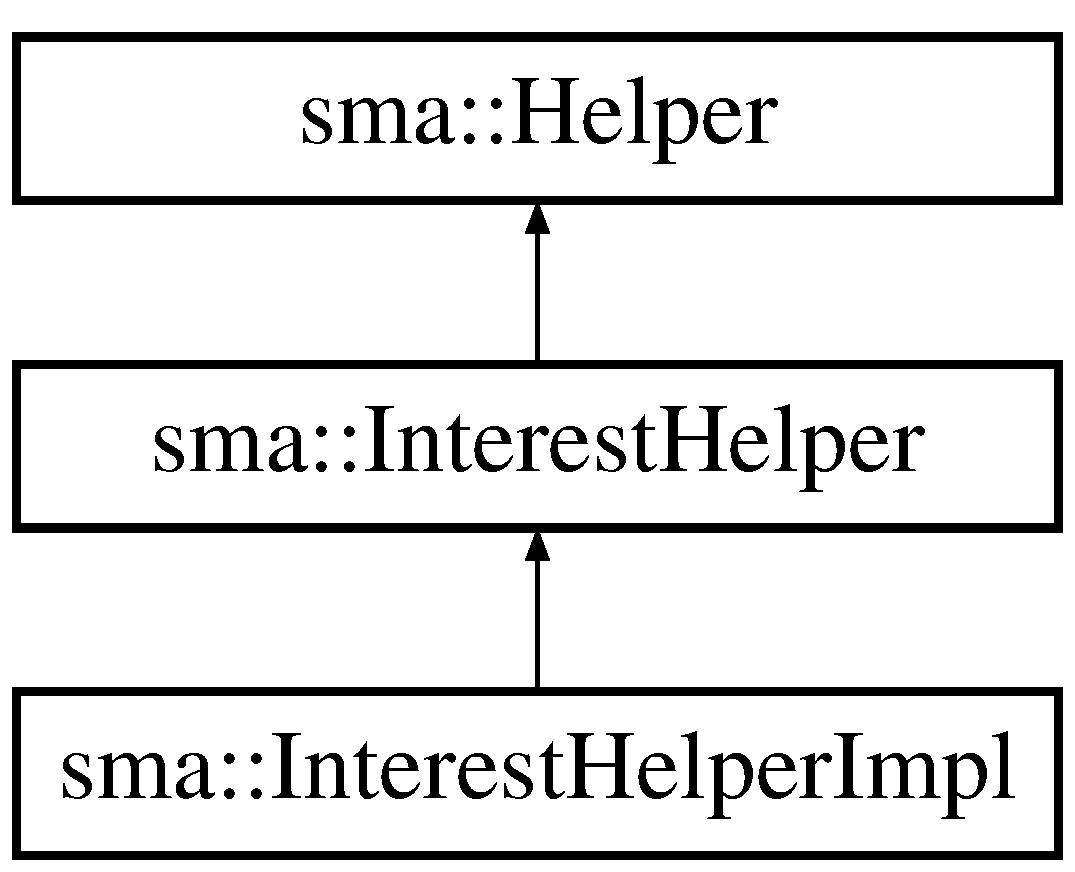
\includegraphics[height=3.000000cm]{classsma_1_1InterestHelper}
\end{center}
\end{figure}
\subsection*{Public Member Functions}
\begin{DoxyCompactItemize}
\item 
\hypertarget{classsma_1_1InterestHelper_a1b8f165aa3922a94d80b50787fc86d8d}{{\bfseries Interest\-Helper} (\hyperlink{classsma_1_1CcnNode}{Ccn\-Node} \&node)}\label{classsma_1_1InterestHelper_a1b8f165aa3922a94d80b50787fc86d8d}

\item 
\hypertarget{classsma_1_1InterestHelper_a4adb1b1209a8623e6551fa06ba6cec4f}{virtual void {\bfseries receive} (\hyperlink{structsma_1_1MessageHeader}{Message\-Header} header, \hyperlink{structsma_1_1InterestAnnouncement}{Interest\-Announcement} msg)=0}\label{classsma_1_1InterestHelper_a4adb1b1209a8623e6551fa06ba6cec4f}

\item 
\hypertarget{classsma_1_1InterestHelper_a1a973f3ba1575c57dc7da86691c07d4f}{virtual void {\bfseries insert\-\_\-new} (std\-::vector$<$ \hyperlink{structsma_1_1ContentType}{Content\-Type} $>$ types)=0}\label{classsma_1_1InterestHelper_a1a973f3ba1575c57dc7da86691c07d4f}

\item 
\hypertarget{classsma_1_1InterestHelper_a433f46b2a5d7af0576cf228fddf92260}{virtual bool {\bfseries interested\-\_\-in} (\hyperlink{structsma_1_1ContentDescriptor}{Content\-Descriptor} const \&descriptor) const =0}\label{classsma_1_1InterestHelper_a433f46b2a5d7af0576cf228fddf92260}

\item 
\hypertarget{classsma_1_1InterestHelper_ad56a3e52c84592088e32f22a1632bc14}{virtual bool {\bfseries know\-\_\-remote} (\hyperlink{structsma_1_1ContentType}{Content\-Type} const \&type) const =0}\label{classsma_1_1InterestHelper_ad56a3e52c84592088e32f22a1632bc14}

\end{DoxyCompactItemize}
\subsection*{Additional Inherited Members}


The documentation for this class was generated from the following files\-:\begin{DoxyCompactItemize}
\item 
include/sma/ccn/interesthelper.\-hpp\item 
src/ccn/interesthelper.\-cpp\end{DoxyCompactItemize}

\hypertarget{classsma_1_1InterestHelperImpl}{\section{sma\-:\-:Interest\-Helper\-Impl Class Reference}
\label{classsma_1_1InterestHelperImpl}\index{sma\-::\-Interest\-Helper\-Impl@{sma\-::\-Interest\-Helper\-Impl}}
}


Manages the storage, announcement, and replication of content interests.  




{\ttfamily \#include $<$interesthelperimpl.\-hpp$>$}

Inheritance diagram for sma\-:\-:Interest\-Helper\-Impl\-:\begin{figure}[H]
\begin{center}
\leavevmode
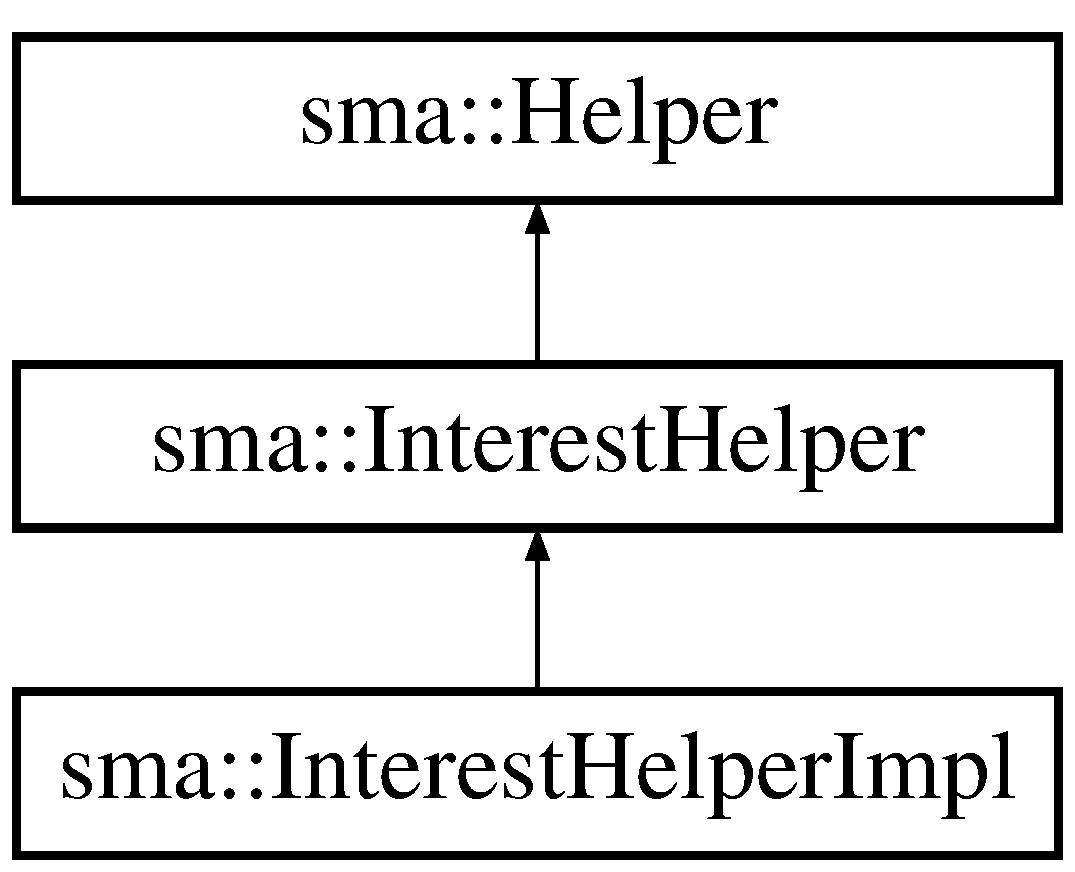
\includegraphics[height=3.000000cm]{classsma_1_1InterestHelperImpl}
\end{center}
\end{figure}
\subsection*{Public Member Functions}
\begin{DoxyCompactItemize}
\item 
\hypertarget{classsma_1_1InterestHelperImpl_a23ad77fcd0a36abd6f2c663570080a82}{\hyperlink{classsma_1_1InterestHelperImpl_a23ad77fcd0a36abd6f2c663570080a82}{Interest\-Helper\-Impl} (\hyperlink{classsma_1_1CcnNode}{Ccn\-Node} \&node)}\label{classsma_1_1InterestHelperImpl_a23ad77fcd0a36abd6f2c663570080a82}

\begin{DoxyCompactList}\small\item\em Construct a helper to manage interests for the given node. \end{DoxyCompactList}\item 
\hypertarget{classsma_1_1InterestHelperImpl_ac85793ecbb9c57e35e5cf73bd9d982ba}{void {\bfseries receive} (\hyperlink{structsma_1_1MessageHeader}{Message\-Header} header, \hyperlink{structsma_1_1InterestAnnouncement}{Interest\-Announcement} msg) override}\label{classsma_1_1InterestHelperImpl_ac85793ecbb9c57e35e5cf73bd9d982ba}

\item 
\hypertarget{classsma_1_1InterestHelperImpl_acb5ea058a96877430a967c3e42208006}{void {\bfseries insert\-\_\-new} (std\-::vector$<$ \hyperlink{structsma_1_1ContentType}{Content\-Type} $>$ types) override}\label{classsma_1_1InterestHelperImpl_acb5ea058a96877430a967c3e42208006}

\item 
\hypertarget{classsma_1_1InterestHelperImpl_a397988adc785d1f8607c0be26c86c5b5}{bool {\bfseries interested\-\_\-in} (\hyperlink{structsma_1_1ContentDescriptor}{Content\-Descriptor} const \&info) const override}\label{classsma_1_1InterestHelperImpl_a397988adc785d1f8607c0be26c86c5b5}

\item 
\hypertarget{classsma_1_1InterestHelperImpl_aedbe0383cd4ba8308b23fb089bb9c399}{bool {\bfseries know\-\_\-remote} (\hyperlink{structsma_1_1ContentType}{Content\-Type} const \&type) const override}\label{classsma_1_1InterestHelperImpl_aedbe0383cd4ba8308b23fb089bb9c399}

\end{DoxyCompactItemize}
\subsection*{Additional Inherited Members}


\subsection{Detailed Description}
Manages the storage, announcement, and replication of content interests. 

Consumers express interest in content in order to become targets of dissemination from remote, unknown, providers.

For provisioned content to reliably reach consumers a majority of nodes should know generally what content are in demand; they can then make intelligent forwarding and caching decisions to facilitate content where it's wanted without completely flooding the network.

While it does appear to be a different sort of flooding, the interest data are intended to be extremely light weight relative to the content metadata and should require a minimum of effort to handle. 

The documentation for this class was generated from the following files\-:\begin{DoxyCompactItemize}
\item 
include/sma/ccn/interesthelperimpl.\-hpp\item 
src/ccn/interesthelperimpl.\-cpp\end{DoxyCompactItemize}

\hypertarget{structsma_1_1InterestRank}{\section{sma\-:\-:Interest\-Rank Struct Reference}
\label{structsma_1_1InterestRank}\index{sma\-::\-Interest\-Rank@{sma\-::\-Interest\-Rank}}
}
\subsection*{Public Member Functions}
\begin{DoxyCompactItemize}
\item 
\hypertarget{structsma_1_1InterestRank_adca7702a3a97a882a7a328b579f9b204}{bool {\bfseries operator==} (\hyperlink{structsma_1_1InterestRank}{Interest\-Rank} const \&r) const }\label{structsma_1_1InterestRank_adca7702a3a97a882a7a328b579f9b204}

\item 
\hypertarget{structsma_1_1InterestRank_a2cf773eb98077660ac05c983c20c9afd}{bool {\bfseries operator!=} (\hyperlink{structsma_1_1InterestRank}{Interest\-Rank} const \&r) const }\label{structsma_1_1InterestRank_a2cf773eb98077660ac05c983c20c9afd}

\item 
\hypertarget{structsma_1_1InterestRank_abc2f757dc8d90c342f241eac2872a872}{bool {\bfseries operator$<$=} (\hyperlink{structsma_1_1InterestRank}{Interest\-Rank} const \&r) const }\label{structsma_1_1InterestRank_abc2f757dc8d90c342f241eac2872a872}

\item 
\hypertarget{structsma_1_1InterestRank_aee2592b5b4f3a49c8da84dfd263c78e3}{bool {\bfseries operator$>$=} (\hyperlink{structsma_1_1InterestRank}{Interest\-Rank} const \&r) const }\label{structsma_1_1InterestRank_aee2592b5b4f3a49c8da84dfd263c78e3}

\item 
\hypertarget{structsma_1_1InterestRank_ad4a93100d17f214a5029d116b0cb7fb5}{bool {\bfseries operator$<$} (\hyperlink{structsma_1_1InterestRank}{Interest\-Rank} const \&r) const }\label{structsma_1_1InterestRank_ad4a93100d17f214a5029d116b0cb7fb5}

\item 
\hypertarget{structsma_1_1InterestRank_a6b64e7469866ef6a871500b0738e7cca}{bool {\bfseries operator$>$} (\hyperlink{structsma_1_1InterestRank}{Interest\-Rank} const \&r) const }\label{structsma_1_1InterestRank_a6b64e7469866ef6a871500b0738e7cca}

\item 
\hypertarget{structsma_1_1InterestRank_ad5cc9fa8e5ac5033eb4155bf52feae81}{{\bfseries operator value\-\_\-type} () const }\label{structsma_1_1InterestRank_ad5cc9fa8e5ac5033eb4155bf52feae81}

\item 
\hypertarget{structsma_1_1InterestRank_acf11198c30e84f46a1eae10b7c10b061}{{\bfseries operator std\-::string} () const }\label{structsma_1_1InterestRank_acf11198c30e84f46a1eae10b7c10b061}

\end{DoxyCompactItemize}
\subsection*{Public Attributes}
\begin{DoxyCompactItemize}
\item 
\hypertarget{structsma_1_1InterestRank_af8c488e3fba2f04c012cb551623ae3aa}{value\-\_\-type {\bfseries value}}\label{structsma_1_1InterestRank_af8c488e3fba2f04c012cb551623ae3aa}

\end{DoxyCompactItemize}
\subsection*{Friends}
\begin{DoxyCompactItemize}
\item 
\hypertarget{structsma_1_1InterestRank_a9469f1565914e71f0a4934b5ff2495fc}{struct {\bfseries std\-::hash$<$ Interest\-Rank $>$}}\label{structsma_1_1InterestRank_a9469f1565914e71f0a4934b5ff2495fc}

\end{DoxyCompactItemize}


The documentation for this struct was generated from the following file\-:\begin{DoxyCompactItemize}
\item 
include/sma/ccn/interestrank.\-hpp\end{DoxyCompactItemize}

\hypertarget{structsma_1_1detail_1_1is__vector}{\section{sma\-:\-:detail\-:\-:is\-\_\-vector$<$ T, typename $>$ Struct Template Reference}
\label{structsma_1_1detail_1_1is__vector}\index{sma\-::detail\-::is\-\_\-vector$<$ T, typename $>$@{sma\-::detail\-::is\-\_\-vector$<$ T, typename $>$}}
}
\subsection*{Static Public Attributes}
\begin{DoxyCompactItemize}
\item 
\hypertarget{structsma_1_1detail_1_1is__vector_a0d0a056b5791ed01b2740666eec70f68}{static constexpr bool {\bfseries value} = false}\label{structsma_1_1detail_1_1is__vector_a0d0a056b5791ed01b2740666eec70f68}

\end{DoxyCompactItemize}


The documentation for this struct was generated from the following file\-:\begin{DoxyCompactItemize}
\item 
include/sma/util/reader.\-hpp\end{DoxyCompactItemize}

\hypertarget{structsma_1_1detail_1_1is__vector_3_01T_00_01typename_01std_1_1enable__if_3_01std_1_1is__same_3_9d34c27f05b3399b2e14e513707d89ed}{\section{sma\-:\-:detail\-:\-:is\-\_\-vector$<$ T, typename std\-:\-:enable\-\_\-if$<$ std\-:\-:is\-\_\-same$<$ T, std\-:\-:vector$<$ typename T\-:\-:value\-\_\-type, typename T\-:\-:allocator\-\_\-type $>$ $>$\-:\-:value $>$\-:\-:type $>$ Struct Template Reference}
\label{structsma_1_1detail_1_1is__vector_3_01T_00_01typename_01std_1_1enable__if_3_01std_1_1is__same_3_9d34c27f05b3399b2e14e513707d89ed}\index{sma\-::detail\-::is\-\_\-vector$<$ T, typename std\-::enable\-\_\-if$<$ std\-::is\-\_\-same$<$ T, std\-::vector$<$ typename T\-::value\-\_\-type, typename T\-::allocator\-\_\-type $>$ $>$\-::value $>$\-::type $>$@{sma\-::detail\-::is\-\_\-vector$<$ T, typename std\-::enable\-\_\-if$<$ std\-::is\-\_\-same$<$ T, std\-::vector$<$ typename T\-::value\-\_\-type, typename T\-::allocator\-\_\-type $>$ $>$\-::value $>$\-::type $>$}}
}
\subsection*{Static Public Attributes}
\begin{DoxyCompactItemize}
\item 
\hypertarget{structsma_1_1detail_1_1is__vector_3_01T_00_01typename_01std_1_1enable__if_3_01std_1_1is__same_3_9d34c27f05b3399b2e14e513707d89ed_ac3520b82ef46f64a090e20df5ac37649}{static constexpr bool {\bfseries value} = true}\label{structsma_1_1detail_1_1is__vector_3_01T_00_01typename_01std_1_1enable__if_3_01std_1_1is__same_3_9d34c27f05b3399b2e14e513707d89ed_ac3520b82ef46f64a090e20df5ac37649}

\end{DoxyCompactItemize}


The documentation for this struct was generated from the following file\-:\begin{DoxyCompactItemize}
\item 
include/sma/util/reader.\-hpp\end{DoxyCompactItemize}

\hypertarget{classel_1_1LevelHelper}{\section{el\-:\-:Level\-Helper Class Reference}
\label{classel_1_1LevelHelper}\index{el\-::\-Level\-Helper@{el\-::\-Level\-Helper}}
}


Static class that contains helper functions for \hyperlink{namespaceel_ab0ac6091262344c52dd2d3ad099e8e36}{el\-::\-Level}.  




{\ttfamily \#include $<$logimpl.\-hpp$>$}

Inheritance diagram for el\-:\-:Level\-Helper\-:\begin{figure}[H]
\begin{center}
\leavevmode
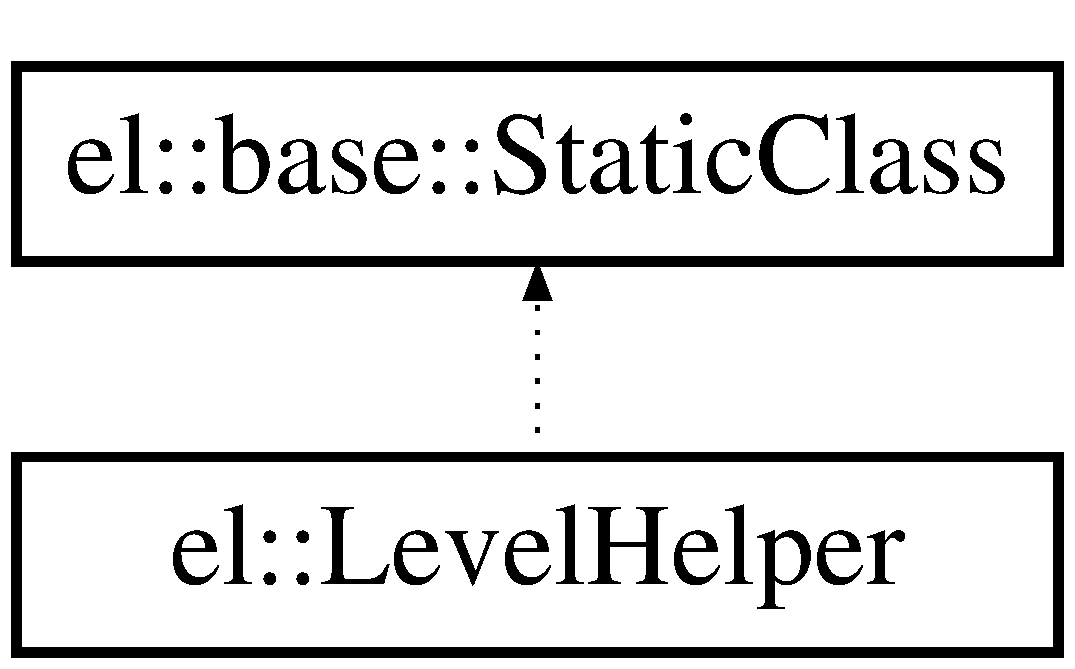
\includegraphics[height=2.000000cm]{classel_1_1LevelHelper}
\end{center}
\end{figure}
\subsection*{Static Public Member Functions}
\begin{DoxyCompactItemize}
\item 
\hypertarget{classel_1_1LevelHelper_a6576fd7cd6d1d839952145115c6e4b38}{static base\-::type\-::\-Enum\-Type \hyperlink{classel_1_1LevelHelper_a6576fd7cd6d1d839952145115c6e4b38}{cast\-To\-Int} (\hyperlink{namespaceel_ab0ac6091262344c52dd2d3ad099e8e36}{Level} level)}\label{classel_1_1LevelHelper_a6576fd7cd6d1d839952145115c6e4b38}

\begin{DoxyCompactList}\small\item\em Casts level to int, useful for iterating through enum. \end{DoxyCompactList}\item 
\hypertarget{classel_1_1LevelHelper_a1279f27df29a003df5ecc3d0bf4dacbb}{static \hyperlink{namespaceel_ab0ac6091262344c52dd2d3ad099e8e36}{Level} \hyperlink{classel_1_1LevelHelper_a1279f27df29a003df5ecc3d0bf4dacbb}{cast\-From\-Int} (base\-::type\-::\-Enum\-Type l)}\label{classel_1_1LevelHelper_a1279f27df29a003df5ecc3d0bf4dacbb}

\begin{DoxyCompactList}\small\item\em Casts int(ushort) to level, useful for iterating through enum. \end{DoxyCompactList}\item 
static const char $\ast$ \hyperlink{classel_1_1LevelHelper_a53b3e226a09af6e87c2072c115b3ba1a}{convert\-To\-String} (\hyperlink{namespaceel_ab0ac6091262344c52dd2d3ad099e8e36}{Level} level)
\begin{DoxyCompactList}\small\item\em Converts level to associated const char$\ast$. \end{DoxyCompactList}\item 
static \hyperlink{namespaceel_ab0ac6091262344c52dd2d3ad099e8e36}{Level} \hyperlink{classel_1_1LevelHelper_a4ff401c62931609c849d580fb6ad2028}{convert\-From\-String} (const char $\ast$level\-Str)
\begin{DoxyCompactList}\small\item\em Converts from level\-Str to Level. \end{DoxyCompactList}\item 
static void \hyperlink{classel_1_1LevelHelper_a953aafa4c876bd673e1e89b0fa57077e}{for\-Each\-Level} (base\-::type\-::\-Enum\-Type $\ast$start\-Index, const std\-::function$<$ bool(void) $>$ \&fn)
\begin{DoxyCompactList}\small\item\em Applies specified function to each level starting from start\-Index. \end{DoxyCompactList}\end{DoxyCompactItemize}
\subsection*{Static Public Attributes}
\begin{DoxyCompactItemize}
\item 
static const base\-::type\-::\-Enum\-Type \hyperlink{classel_1_1LevelHelper_a3ecfe43d5b242e9946bad7f61ea4d89d}{k\-Min\-Valid}
\begin{DoxyCompactList}\small\item\em Represents minimum valid level. Useful when iterating through enum. \end{DoxyCompactList}\item 
static const base\-::type\-::\-Enum\-Type \hyperlink{classel_1_1LevelHelper_aa06e80c65db5c336c4aad25872cf9a48}{k\-Max\-Valid}
\begin{DoxyCompactList}\small\item\em Represents maximum valid level. This is used internally and you should not need it. \end{DoxyCompactList}\end{DoxyCompactItemize}


\subsection{Detailed Description}
Static class that contains helper functions for \hyperlink{namespaceel_ab0ac6091262344c52dd2d3ad099e8e36}{el\-::\-Level}. 

\subsection{Member Function Documentation}
\hypertarget{classel_1_1LevelHelper_a4ff401c62931609c849d580fb6ad2028}{\index{el\-::\-Level\-Helper@{el\-::\-Level\-Helper}!convert\-From\-String@{convert\-From\-String}}
\index{convert\-From\-String@{convert\-From\-String}!el::LevelHelper@{el\-::\-Level\-Helper}}
\subsubsection[{convert\-From\-String}]{\setlength{\rightskip}{0pt plus 5cm}static {\bf Level} el\-::\-Level\-Helper\-::convert\-From\-String (
\begin{DoxyParamCaption}
\item[{const char $\ast$}]{level\-Str}
\end{DoxyParamCaption}
)\hspace{0.3cm}{\ttfamily [inline]}, {\ttfamily [static]}}}\label{classel_1_1LevelHelper_a4ff401c62931609c849d580fb6ad2028}


Converts from level\-Str to Level. 


\begin{DoxyParams}{Parameters}
{\em level\-Str} & Upper case string based level. Lower case is also valid but providing upper case is recommended. \\
\hline
\end{DoxyParams}
\hypertarget{classel_1_1LevelHelper_a53b3e226a09af6e87c2072c115b3ba1a}{\index{el\-::\-Level\-Helper@{el\-::\-Level\-Helper}!convert\-To\-String@{convert\-To\-String}}
\index{convert\-To\-String@{convert\-To\-String}!el::LevelHelper@{el\-::\-Level\-Helper}}
\subsubsection[{convert\-To\-String}]{\setlength{\rightskip}{0pt plus 5cm}static const char$\ast$ el\-::\-Level\-Helper\-::convert\-To\-String (
\begin{DoxyParamCaption}
\item[{{\bf Level}}]{level}
\end{DoxyParamCaption}
)\hspace{0.3cm}{\ttfamily [inline]}, {\ttfamily [static]}}}\label{classel_1_1LevelHelper_a53b3e226a09af6e87c2072c115b3ba1a}


Converts level to associated const char$\ast$. 

\begin{DoxyReturn}{Returns}
Upper case string based level. 
\end{DoxyReturn}
\hypertarget{classel_1_1LevelHelper_a953aafa4c876bd673e1e89b0fa57077e}{\index{el\-::\-Level\-Helper@{el\-::\-Level\-Helper}!for\-Each\-Level@{for\-Each\-Level}}
\index{for\-Each\-Level@{for\-Each\-Level}!el::LevelHelper@{el\-::\-Level\-Helper}}
\subsubsection[{for\-Each\-Level}]{\setlength{\rightskip}{0pt plus 5cm}static void el\-::\-Level\-Helper\-::for\-Each\-Level (
\begin{DoxyParamCaption}
\item[{base\-::type\-::\-Enum\-Type $\ast$}]{start\-Index, }
\item[{const std\-::function$<$ bool(void) $>$ \&}]{fn}
\end{DoxyParamCaption}
)\hspace{0.3cm}{\ttfamily [inline]}, {\ttfamily [static]}}}\label{classel_1_1LevelHelper_a953aafa4c876bd673e1e89b0fa57077e}


Applies specified function to each level starting from start\-Index. 


\begin{DoxyParams}{Parameters}
{\em start\-Index} & initial value to start the iteration from. This is passed as pointer and is left-\/shifted so this can be used inside function (fn) to represent current level. \\
\hline
{\em fn} & function to apply with each level. This bool represent whether or not to stop iterating through levels. \\
\hline
\end{DoxyParams}


\subsection{Member Data Documentation}
\hypertarget{classel_1_1LevelHelper_aa06e80c65db5c336c4aad25872cf9a48}{\index{el\-::\-Level\-Helper@{el\-::\-Level\-Helper}!k\-Max\-Valid@{k\-Max\-Valid}}
\index{k\-Max\-Valid@{k\-Max\-Valid}!el::LevelHelper@{el\-::\-Level\-Helper}}
\subsubsection[{k\-Max\-Valid}]{\setlength{\rightskip}{0pt plus 5cm}const base\-::type\-::\-Enum\-Type el\-::\-Level\-Helper\-::k\-Max\-Valid\hspace{0.3cm}{\ttfamily [static]}}}\label{classel_1_1LevelHelper_aa06e80c65db5c336c4aad25872cf9a48}
{\bfseries Initial value\-:}
\begin{DoxyCode}
=
      \textcolor{keyword}{static\_cast<}base::type::EnumType\textcolor{keyword}{>}(\hyperlink{namespaceel_ab0ac6091262344c52dd2d3ad099e8e36a4059b0251f66a18cb56f544728796875}{Level::Info})
\end{DoxyCode}


Represents maximum valid level. This is used internally and you should not need it. 

\hypertarget{classel_1_1LevelHelper_a3ecfe43d5b242e9946bad7f61ea4d89d}{\index{el\-::\-Level\-Helper@{el\-::\-Level\-Helper}!k\-Min\-Valid@{k\-Min\-Valid}}
\index{k\-Min\-Valid@{k\-Min\-Valid}!el::LevelHelper@{el\-::\-Level\-Helper}}
\subsubsection[{k\-Min\-Valid}]{\setlength{\rightskip}{0pt plus 5cm}const base\-::type\-::\-Enum\-Type el\-::\-Level\-Helper\-::k\-Min\-Valid\hspace{0.3cm}{\ttfamily [static]}}}\label{classel_1_1LevelHelper_a3ecfe43d5b242e9946bad7f61ea4d89d}
{\bfseries Initial value\-:}
\begin{DoxyCode}
=
      \textcolor{keyword}{static\_cast<}base::type::EnumType\textcolor{keyword}{>}(\hyperlink{namespaceel_ab0ac6091262344c52dd2d3ad099e8e36add4ec0ac4e58f7c32a01244ae91150b1}{Level::Trace})
\end{DoxyCode}


Represents minimum valid level. Useful when iterating through enum. 



The documentation for this class was generated from the following file\-:\begin{DoxyCompactItemize}
\item 
include/sma/io/detail/logimpl.\-hpp\end{DoxyCompactItemize}

\hypertarget{classsma_1_1Link}{\section{sma\-:\-:Link Class Reference}
\label{classsma_1_1Link}\index{sma\-::\-Link@{sma\-::\-Link}}
}
Inheritance diagram for sma\-:\-:Link\-:\begin{figure}[H]
\begin{center}
\leavevmode
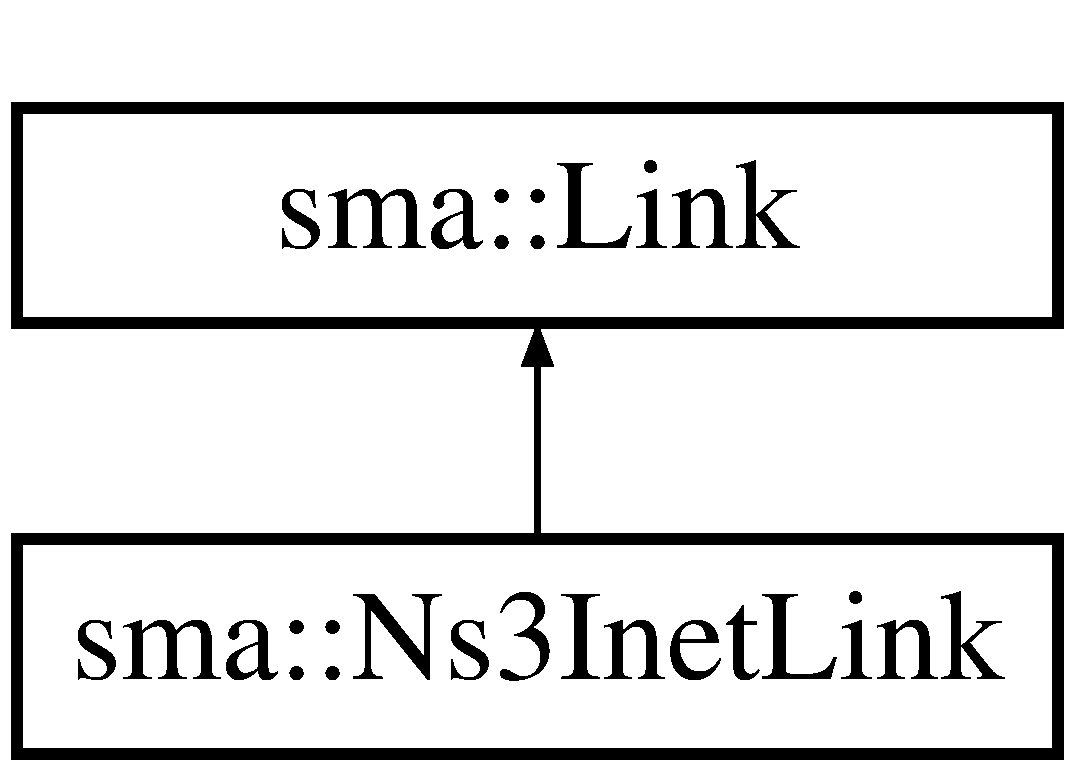
\includegraphics[height=2.000000cm]{classsma_1_1Link}
\end{center}
\end{figure}
\subsection*{Public Member Functions}
\begin{DoxyCompactItemize}
\item 
\hypertarget{classsma_1_1Link_aa41c72ed9f74728df6c0dda4730af198}{{\bfseries Link} (\hyperlink{classsma_1_1Link}{Link} const \&)=delete}\label{classsma_1_1Link_aa41c72ed9f74728df6c0dda4730af198}

\item 
\hypertarget{classsma_1_1Link_ab778fe1e2040195082814ef9e851669e}{\hyperlink{classsma_1_1Link}{Link} \& {\bfseries operator=} (\hyperlink{classsma_1_1Link}{Link} const \&)=delete}\label{classsma_1_1Link_ab778fe1e2040195082814ef9e851669e}

\item 
\hypertarget{classsma_1_1Link_ae78ebf16997f24cca6ca4d76ddffa3c4}{void {\bfseries receive\-\_\-to} (\hyperlink{classsma_1_1LinkLayer}{Link\-Layer} \&ll)}\label{classsma_1_1Link_ae78ebf16997f24cca6ca4d76ddffa3c4}

\item 
\hypertarget{classsma_1_1Link_ac7ab2e31016fbdce38147354112d625d}{bool {\bfseries readable} ()}\label{classsma_1_1Link_ac7ab2e31016fbdce38147354112d625d}

\item 
\hypertarget{classsma_1_1Link_a0b4b817cc3fa0d8ce46e11fa0719b600}{virtual std\-::size\-\_\-t {\bfseries read} (void $\ast$dst, std\-::size\-\_\-t size)=0}\label{classsma_1_1Link_a0b4b817cc3fa0d8ce46e11fa0719b600}

\item 
\hypertarget{classsma_1_1Link_a1b81ed7fa62cb16c9eef3d7c1298815f}{virtual std\-::size\-\_\-t {\bfseries write} (void const $\ast$src, std\-::size\-\_\-t size)=0}\label{classsma_1_1Link_a1b81ed7fa62cb16c9eef3d7c1298815f}

\item 
\hypertarget{classsma_1_1Link_a35f866adef2421b35b9d62cd44af6241}{virtual void {\bfseries close} ()=0}\label{classsma_1_1Link_a35f866adef2421b35b9d62cd44af6241}

\end{DoxyCompactItemize}
\subsection*{Protected Member Functions}
\begin{DoxyCompactItemize}
\item 
\hypertarget{classsma_1_1Link_ab0cd9db02000b582c5f8e770b1cec242}{void {\bfseries readable} (bool r)}\label{classsma_1_1Link_ab0cd9db02000b582c5f8e770b1cec242}

\end{DoxyCompactItemize}


The documentation for this class was generated from the following files\-:\begin{DoxyCompactItemize}
\item 
include/sma/link.\-hpp\item 
src/link.\-cpp\end{DoxyCompactItemize}

\hypertarget{classsma_1_1LinkLayer}{\section{sma\-:\-:Link\-Layer Class Reference}
\label{classsma_1_1LinkLayer}\index{sma\-::\-Link\-Layer@{sma\-::\-Link\-Layer}}
}
Inheritance diagram for sma\-:\-:Link\-Layer\-:\begin{figure}[H]
\begin{center}
\leavevmode
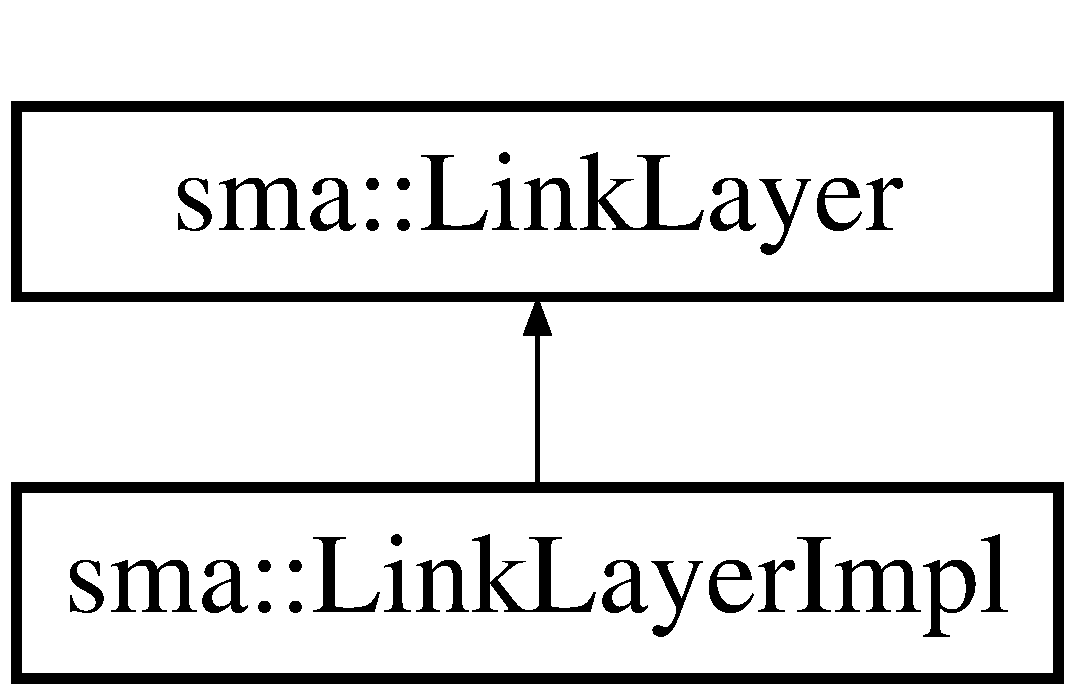
\includegraphics[height=2.000000cm]{classsma_1_1LinkLayer}
\end{center}
\end{figure}
\subsection*{Public Member Functions}
\begin{DoxyCompactItemize}
\item 
\hypertarget{classsma_1_1LinkLayer_a1b66460173365ef6133b983421fe7bb9}{{\bfseries Link\-Layer} (\hyperlink{classsma_1_1LinkLayer}{Link\-Layer} const \&r)=delete}\label{classsma_1_1LinkLayer_a1b66460173365ef6133b983421fe7bb9}

\item 
\hypertarget{classsma_1_1LinkLayer_a2058e2c88d9f67b49561f2196631a91d}{\hyperlink{classsma_1_1LinkLayer}{Link\-Layer} \& {\bfseries operator=} (\hyperlink{classsma_1_1LinkLayer}{Link\-Layer} const \&r)=delete}\label{classsma_1_1LinkLayer_a2058e2c88d9f67b49561f2196631a91d}

\item 
\hypertarget{classsma_1_1LinkLayer_a151cdb38db1e95fe67e215a9cefa7168}{void \hyperlink{classsma_1_1LinkLayer_a151cdb38db1e95fe67e215a9cefa7168}{receive\-\_\-to} (\hyperlink{classsma_1_1CcnNode}{Ccn\-Node} \&\hyperlink{classsma_1_1LinkLayer_af1c41f5c6906c2be5757d4a615f3324a}{node})}\label{classsma_1_1LinkLayer_a151cdb38db1e95fe67e215a9cefa7168}

\begin{DoxyCompactList}\small\item\em Set the node that will receive messages received by the link layer. \end{DoxyCompactList}\item 
\hyperlink{classsma_1_1LinkLayer}{Link\-Layer} \& \hyperlink{classsma_1_1LinkLayer_af3c4ce4bed281e14bbc676988b5acc31}{forward\-\_\-strategy} (\hyperlink{classsma_1_1ForwardStrategy}{Forward\-Strategy} \&strategy)
\begin{DoxyCompactList}\small\item\em Set the strategy used to manage the outgoing message queue. \end{DoxyCompactList}\item 
\hypertarget{classsma_1_1LinkLayer_aff0a6b5cf4c38b7658682b7d6fcc8a34}{virtual void \hyperlink{classsma_1_1LinkLayer_aff0a6b5cf4c38b7658682b7d6fcc8a34}{stop} ()=0}\label{classsma_1_1LinkLayer_aff0a6b5cf4c38b7658682b7d6fcc8a34}

\begin{DoxyCompactList}\small\item\em Gracefully stop communication between the node and the links. \end{DoxyCompactList}\item 
virtual std\-::size\-\_\-t \hyperlink{classsma_1_1LinkLayer_a5e779ec9a213244990374df07906985c}{forward\-\_\-one} ()=0
\begin{DoxyCompactList}\small\item\em Forward the next queued outgoing message to the network. \end{DoxyCompactList}\item 
\hypertarget{classsma_1_1LinkLayer_a4b183144bf01d5e4ed2f7c8f4a6f7231}{virtual void \hyperlink{classsma_1_1LinkLayer_a4b183144bf01d5e4ed2f7c8f4a6f7231}{enqueue} (void const $\ast$src, std\-::size\-\_\-t size)=0}\label{classsma_1_1LinkLayer_a4b183144bf01d5e4ed2f7c8f4a6f7231}

\begin{DoxyCompactList}\small\item\em Place the message in the outgoing message queue. \end{DoxyCompactList}\end{DoxyCompactItemize}
\subsection*{Protected Attributes}
\begin{DoxyCompactItemize}
\item 
\hypertarget{classsma_1_1LinkLayer_af1c41f5c6906c2be5757d4a615f3324a}{\hyperlink{classsma_1_1CcnNode}{Ccn\-Node} $\ast$ \hyperlink{classsma_1_1LinkLayer_af1c41f5c6906c2be5757d4a615f3324a}{node} \{nullptr\}}\label{classsma_1_1LinkLayer_af1c41f5c6906c2be5757d4a615f3324a}

\begin{DoxyCompactList}\small\item\em The target of incoming messages. \end{DoxyCompactList}\item 
\hyperlink{classsma_1_1ForwardStrategy}{Forward\-Strategy} $\ast$ \hyperlink{classsma_1_1LinkLayer_abc5610d847fa48661a6ee79d6872181b}{fwd\-\_\-strat} = nullptr
\begin{DoxyCompactList}\small\item\em The strategy for forwarding outgoing messages to the network. \end{DoxyCompactList}\end{DoxyCompactItemize}
\subsection*{Friends}
\begin{DoxyCompactItemize}
\item 
\hypertarget{classsma_1_1LinkLayer_a1e9ca4d39ca75620494c1f03ae5b00e8}{class {\bfseries Link}}\label{classsma_1_1LinkLayer_a1e9ca4d39ca75620494c1f03ae5b00e8}

\end{DoxyCompactItemize}


\subsection{Member Function Documentation}
\hypertarget{classsma_1_1LinkLayer_a5e779ec9a213244990374df07906985c}{\index{sma\-::\-Link\-Layer@{sma\-::\-Link\-Layer}!forward\-\_\-one@{forward\-\_\-one}}
\index{forward\-\_\-one@{forward\-\_\-one}!sma::LinkLayer@{sma\-::\-Link\-Layer}}
\subsubsection[{forward\-\_\-one}]{\setlength{\rightskip}{0pt plus 5cm}virtual std\-::size\-\_\-t sma\-::\-Link\-Layer\-::forward\-\_\-one (
\begin{DoxyParamCaption}
{}
\end{DoxyParamCaption}
)\hspace{0.3cm}{\ttfamily [pure virtual]}}}\label{classsma_1_1LinkLayer_a5e779ec9a213244990374df07906985c}


Forward the next queued outgoing message to the network. 

\begin{DoxyReturn}{Returns}
the number of queued messages remaining. 
\end{DoxyReturn}


Implemented in \hyperlink{classsma_1_1LinkLayerImpl_a361fbd3e20dd514157a9c088449adf2d}{sma\-::\-Link\-Layer\-Impl}.

\hypertarget{classsma_1_1LinkLayer_af3c4ce4bed281e14bbc676988b5acc31}{\index{sma\-::\-Link\-Layer@{sma\-::\-Link\-Layer}!forward\-\_\-strategy@{forward\-\_\-strategy}}
\index{forward\-\_\-strategy@{forward\-\_\-strategy}!sma::LinkLayer@{sma\-::\-Link\-Layer}}
\subsubsection[{forward\-\_\-strategy}]{\setlength{\rightskip}{0pt plus 5cm}{\bf Link\-Layer}\& sma\-::\-Link\-Layer\-::forward\-\_\-strategy (
\begin{DoxyParamCaption}
\item[{{\bf Forward\-Strategy} \&}]{strategy}
\end{DoxyParamCaption}
)\hspace{0.3cm}{\ttfamily [inline]}}}\label{classsma_1_1LinkLayer_af3c4ce4bed281e14bbc676988b5acc31}


Set the strategy used to manage the outgoing message queue. 

If a forwarding strategy is set, it will be invoked after an outgoing message is buffered and must call the link layer's {\itshape forward\-\_\-one} method to send the message. 

\subsection{Member Data Documentation}
\hypertarget{classsma_1_1LinkLayer_abc5610d847fa48661a6ee79d6872181b}{\index{sma\-::\-Link\-Layer@{sma\-::\-Link\-Layer}!fwd\-\_\-strat@{fwd\-\_\-strat}}
\index{fwd\-\_\-strat@{fwd\-\_\-strat}!sma::LinkLayer@{sma\-::\-Link\-Layer}}
\subsubsection[{fwd\-\_\-strat}]{\setlength{\rightskip}{0pt plus 5cm}{\bf Forward\-Strategy}$\ast$ sma\-::\-Link\-Layer\-::fwd\-\_\-strat = nullptr\hspace{0.3cm}{\ttfamily [protected]}}}\label{classsma_1_1LinkLayer_abc5610d847fa48661a6ee79d6872181b}


The strategy for forwarding outgoing messages to the network. 

Naive blasting to contended networks will cause avoidable loss. The strategy should make intelligent decisions to share the network capacity with other peers. 

The documentation for this class was generated from the following file\-:\begin{DoxyCompactItemize}
\item 
include/sma/linklayer.\-hpp\end{DoxyCompactItemize}

\hypertarget{classsma_1_1LinkLayerImpl}{\section{sma\-:\-:Link\-Layer\-Impl Class Reference}
\label{classsma_1_1LinkLayerImpl}\index{sma\-::\-Link\-Layer\-Impl@{sma\-::\-Link\-Layer\-Impl}}
}
Inheritance diagram for sma\-:\-:Link\-Layer\-Impl\-:\begin{figure}[H]
\begin{center}
\leavevmode
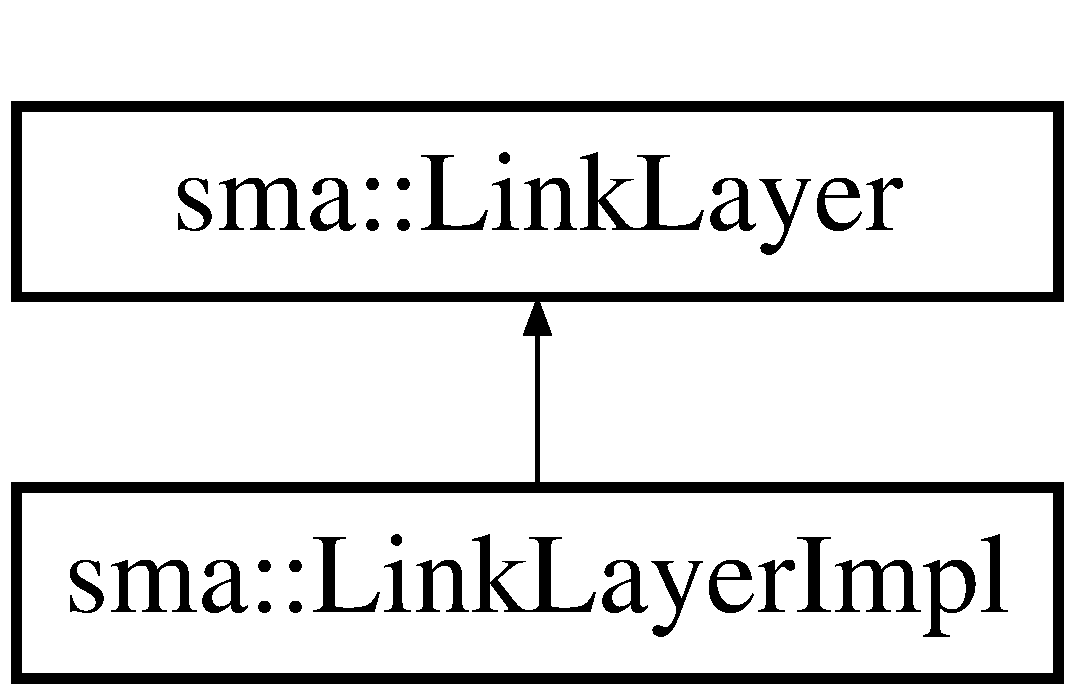
\includegraphics[height=2.000000cm]{classsma_1_1LinkLayerImpl}
\end{center}
\end{figure}
\subsection*{Public Member Functions}
\begin{DoxyCompactItemize}
\item 
\hyperlink{classsma_1_1LinkLayerImpl_afb0d29b2c0897b87ee9508ce087a64e3}{Link\-Layer\-Impl} (std\-::vector$<$ std\-::unique\-\_\-ptr$<$ \hyperlink{classsma_1_1Link}{Link} $>$$>$ links)
\begin{DoxyCompactList}\small\item\em Construct a link layer composed of the given links. \end{DoxyCompactList}\item 
\hypertarget{classsma_1_1LinkLayerImpl_a106dd9f342d57a5b8de01f6f5be6259b}{\hyperlink{classsma_1_1LinkLayerImpl_a106dd9f342d57a5b8de01f6f5be6259b}{Link\-Layer\-Impl} (\hyperlink{classsma_1_1LinkLayerImpl}{Link\-Layer\-Impl} const \&r)=delete}\label{classsma_1_1LinkLayerImpl_a106dd9f342d57a5b8de01f6f5be6259b}

\begin{DoxyCompactList}\small\item\em Copying is disabled because the underlying links are non-\/copyable. \end{DoxyCompactList}\item 
\hypertarget{classsma_1_1LinkLayerImpl_af78279815467ea6f524d5668f661fe16}{\hyperlink{classsma_1_1LinkLayerImpl}{Link\-Layer\-Impl} \& \hyperlink{classsma_1_1LinkLayerImpl_af78279815467ea6f524d5668f661fe16}{operator=} (\hyperlink{classsma_1_1LinkLayerImpl}{Link\-Layer\-Impl} const \&r)=delete}\label{classsma_1_1LinkLayerImpl_af78279815467ea6f524d5668f661fe16}

\begin{DoxyCompactList}\small\item\em Copying is disabled because the underlying links are non-\/copyable. \end{DoxyCompactList}\item 
\hypertarget{classsma_1_1LinkLayerImpl_a22ee25f96b81111f5e780f617651e3bb}{void \hyperlink{classsma_1_1LinkLayerImpl_a22ee25f96b81111f5e780f617651e3bb}{stop} () override}\label{classsma_1_1LinkLayerImpl_a22ee25f96b81111f5e780f617651e3bb}

\begin{DoxyCompactList}\small\item\em Gracefully stop communication between the node and the links. \end{DoxyCompactList}\item 
std\-::size\-\_\-t \hyperlink{classsma_1_1LinkLayerImpl_a361fbd3e20dd514157a9c088449adf2d}{forward\-\_\-one} () override
\begin{DoxyCompactList}\small\item\em Forward the next queued outgoing message to the network. \end{DoxyCompactList}\item 
\hypertarget{classsma_1_1LinkLayerImpl_ab9fa90a70647957b44c514f7278d6d27}{void \hyperlink{classsma_1_1LinkLayerImpl_ab9fa90a70647957b44c514f7278d6d27}{enqueue} (void const $\ast$src, std\-::size\-\_\-t size) override}\label{classsma_1_1LinkLayerImpl_ab9fa90a70647957b44c514f7278d6d27}

\begin{DoxyCompactList}\small\item\em Place the message in the outgoing message queue. \end{DoxyCompactList}\end{DoxyCompactItemize}
\subsection*{Additional Inherited Members}


\subsection{Constructor \& Destructor Documentation}
\hypertarget{classsma_1_1LinkLayerImpl_afb0d29b2c0897b87ee9508ce087a64e3}{\index{sma\-::\-Link\-Layer\-Impl@{sma\-::\-Link\-Layer\-Impl}!Link\-Layer\-Impl@{Link\-Layer\-Impl}}
\index{Link\-Layer\-Impl@{Link\-Layer\-Impl}!sma::LinkLayerImpl@{sma\-::\-Link\-Layer\-Impl}}
\subsubsection[{Link\-Layer\-Impl}]{\setlength{\rightskip}{0pt plus 5cm}sma\-::\-Link\-Layer\-Impl\-::\-Link\-Layer\-Impl (
\begin{DoxyParamCaption}
\item[{std\-::vector$<$ std\-::unique\-\_\-ptr$<$ {\bf Link} $>$$>$}]{links}
\end{DoxyParamCaption}
)}}\label{classsma_1_1LinkLayerImpl_afb0d29b2c0897b87ee9508ce087a64e3}


Construct a link layer composed of the given links. 

The link layer owns its links and they should not be mutated by any other object during its lifetime. 

\subsection{Member Function Documentation}
\hypertarget{classsma_1_1LinkLayerImpl_a361fbd3e20dd514157a9c088449adf2d}{\index{sma\-::\-Link\-Layer\-Impl@{sma\-::\-Link\-Layer\-Impl}!forward\-\_\-one@{forward\-\_\-one}}
\index{forward\-\_\-one@{forward\-\_\-one}!sma::LinkLayerImpl@{sma\-::\-Link\-Layer\-Impl}}
\subsubsection[{forward\-\_\-one}]{\setlength{\rightskip}{0pt plus 5cm}std\-::size\-\_\-t sma\-::\-Link\-Layer\-Impl\-::forward\-\_\-one (
\begin{DoxyParamCaption}
{}
\end{DoxyParamCaption}
)\hspace{0.3cm}{\ttfamily [override]}, {\ttfamily [virtual]}}}\label{classsma_1_1LinkLayerImpl_a361fbd3e20dd514157a9c088449adf2d}


Forward the next queued outgoing message to the network. 

\begin{DoxyReturn}{Returns}
the number of queued messages remaining. 
\end{DoxyReturn}


Implements \hyperlink{classsma_1_1LinkLayer_a5e779ec9a213244990374df07906985c}{sma\-::\-Link\-Layer}.



The documentation for this class was generated from the following files\-:\begin{DoxyCompactItemize}
\item 
include/sma/linklayerimpl.\-hpp\item 
src/linklayerimpl.\-cpp\end{DoxyCompactItemize}

\hypertarget{classel_1_1LogBuilder}{\section{el\-:\-:Log\-Builder Class Reference}
\label{classel_1_1LogBuilder}\index{el\-::\-Log\-Builder@{el\-::\-Log\-Builder}}
}
Inheritance diagram for el\-:\-:Log\-Builder\-:\begin{figure}[H]
\begin{center}
\leavevmode
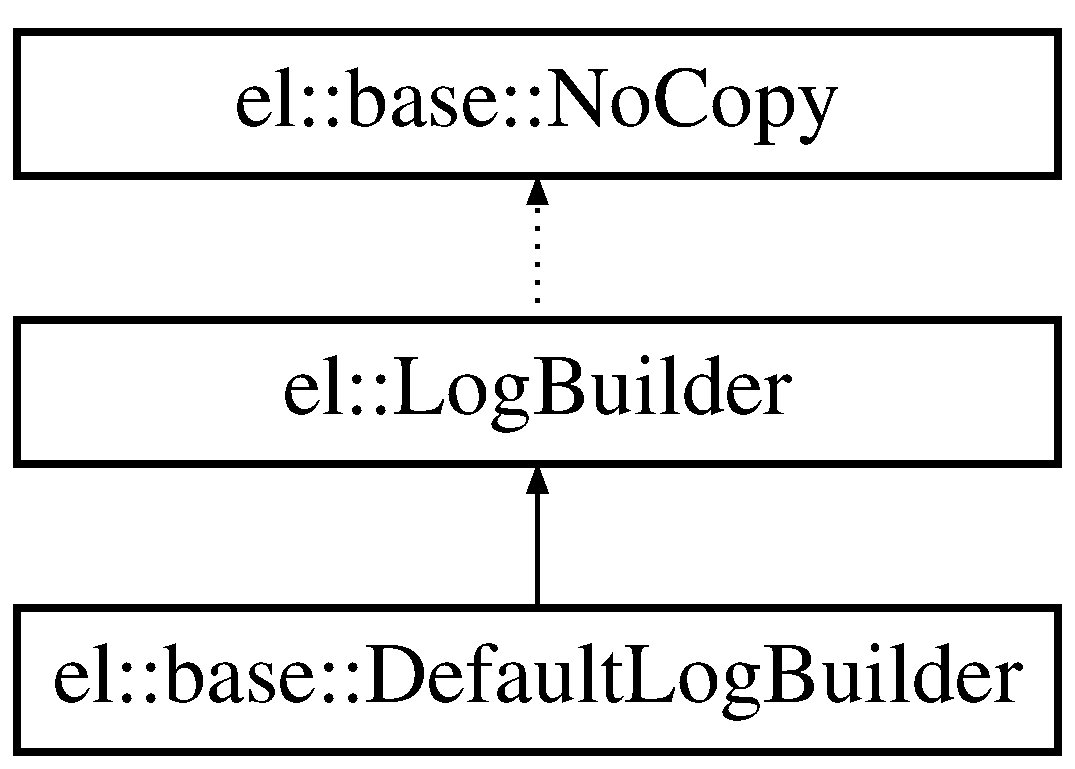
\includegraphics[height=3.000000cm]{classel_1_1LogBuilder}
\end{center}
\end{figure}
\subsection*{Public Member Functions}
\begin{DoxyCompactItemize}
\item 
\hypertarget{classel_1_1LogBuilder_a633b373a3bb9d3e17bdd664aeba4dbc8}{virtual base\-::type\-::string\-\_\-t {\bfseries build} (const \hyperlink{classel_1_1LogMessage}{Log\-Message} $\ast$log\-Message, bool append\-New\-Line) const =0}\label{classel_1_1LogBuilder_a633b373a3bb9d3e17bdd664aeba4dbc8}

\end{DoxyCompactItemize}
\subsection*{Friends}
\begin{DoxyCompactItemize}
\item 
\hypertarget{classel_1_1LogBuilder_a42b1de96d584ae4fecbfc2b9aff95052}{class {\bfseries el\-::base\-::\-Default\-Log\-Dispatch\-Callback}}\label{classel_1_1LogBuilder_a42b1de96d584ae4fecbfc2b9aff95052}

\end{DoxyCompactItemize}


The documentation for this class was generated from the following file\-:\begin{DoxyCompactItemize}
\item 
include/sma/io/detail/logimpl.\-hpp\end{DoxyCompactItemize}

\hypertarget{classel_1_1LogDispatchCallback}{\section{el\-:\-:Log\-Dispatch\-Callback Class Reference}
\label{classel_1_1LogDispatchCallback}\index{el\-::\-Log\-Dispatch\-Callback@{el\-::\-Log\-Dispatch\-Callback}}
}
Inheritance diagram for el\-:\-:Log\-Dispatch\-Callback\-:\begin{figure}[H]
\begin{center}
\leavevmode
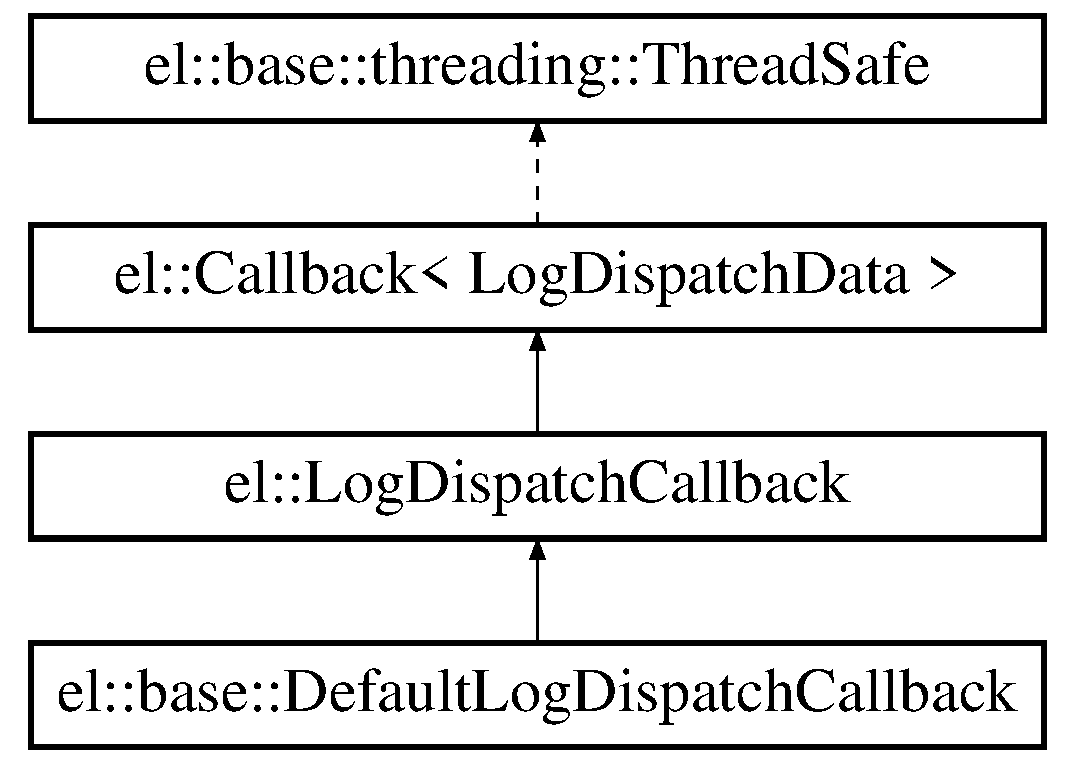
\includegraphics[height=4.000000cm]{classel_1_1LogDispatchCallback}
\end{center}
\end{figure}
\subsection*{Friends}
\begin{DoxyCompactItemize}
\item 
\hypertarget{classel_1_1LogDispatchCallback_a84d22f9ad5b796e49ff5f15a8c32773d}{class {\bfseries base\-::\-Log\-Dispatcher}}\label{classel_1_1LogDispatchCallback_a84d22f9ad5b796e49ff5f15a8c32773d}

\end{DoxyCompactItemize}
\subsection*{Additional Inherited Members}


The documentation for this class was generated from the following file\-:\begin{DoxyCompactItemize}
\item 
include/sma/io/detail/logimpl.\-hpp\end{DoxyCompactItemize}

\hypertarget{classel_1_1LogDispatchData}{\section{el\-:\-:Log\-Dispatch\-Data Class Reference}
\label{classel_1_1LogDispatchData}\index{el\-::\-Log\-Dispatch\-Data@{el\-::\-Log\-Dispatch\-Data}}
}
\subsection*{Public Member Functions}
\begin{DoxyCompactItemize}
\item 
\hypertarget{classel_1_1LogDispatchData_ad52d4ddc330b6260bf10e9879a653829}{const \hyperlink{classel_1_1LogMessage}{Log\-Message} $\ast$ {\bfseries log\-Message} (void) const }\label{classel_1_1LogDispatchData_ad52d4ddc330b6260bf10e9879a653829}

\item 
\hypertarget{classel_1_1LogDispatchData_aee0808c660aa39b34ee69850a2c74c09}{\hyperlink{namespaceel_1_1base_a3aa2563d38e47388ba242a1694fc2839}{base\-::\-Dispatch\-Action} {\bfseries dispatch\-Action} (void) const }\label{classel_1_1LogDispatchData_aee0808c660aa39b34ee69850a2c74c09}

\end{DoxyCompactItemize}
\subsection*{Friends}
\begin{DoxyCompactItemize}
\item 
\hypertarget{classel_1_1LogDispatchData_a84d22f9ad5b796e49ff5f15a8c32773d}{class {\bfseries base\-::\-Log\-Dispatcher}}\label{classel_1_1LogDispatchData_a84d22f9ad5b796e49ff5f15a8c32773d}

\end{DoxyCompactItemize}


The documentation for this class was generated from the following file\-:\begin{DoxyCompactItemize}
\item 
include/sma/io/detail/logimpl.\-hpp\end{DoxyCompactItemize}

\hypertarget{classel_1_1base_1_1LogDispatcher}{\section{el\-:\-:base\-:\-:Log\-Dispatcher Class Reference}
\label{classel_1_1base_1_1LogDispatcher}\index{el\-::base\-::\-Log\-Dispatcher@{el\-::base\-::\-Log\-Dispatcher}}
}


Dispatches log messages.  




{\ttfamily \#include $<$logimpl.\-hpp$>$}

Inheritance diagram for el\-:\-:base\-:\-:Log\-Dispatcher\-:\begin{figure}[H]
\begin{center}
\leavevmode
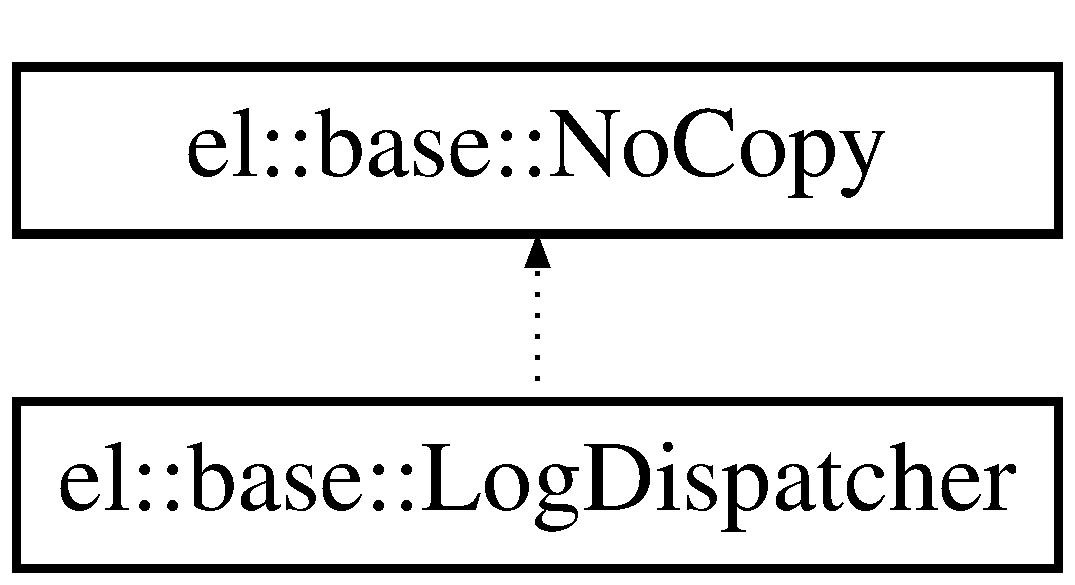
\includegraphics[height=2.000000cm]{classel_1_1base_1_1LogDispatcher}
\end{center}
\end{figure}
\subsection*{Public Member Functions}
\begin{DoxyCompactItemize}
\item 
\hypertarget{classel_1_1base_1_1LogDispatcher_aef59d9895c348f0b3ad5a776276f1c22}{{\bfseries Log\-Dispatcher} (bool proceed, \hyperlink{classel_1_1LogMessage}{Log\-Message} \&\&log\-Message, \hyperlink{namespaceel_1_1base_a3aa2563d38e47388ba242a1694fc2839}{base\-::\-Dispatch\-Action} dispatch\-Action)}\label{classel_1_1base_1_1LogDispatcher_aef59d9895c348f0b3ad5a776276f1c22}

\item 
\hypertarget{classel_1_1base_1_1LogDispatcher_a88d4a644364bb454136c85338f05da7a}{void {\bfseries dispatch} (void)}\label{classel_1_1base_1_1LogDispatcher_a88d4a644364bb454136c85338f05da7a}

\end{DoxyCompactItemize}


\subsection{Detailed Description}
Dispatches log messages. 

The documentation for this class was generated from the following file\-:\begin{DoxyCompactItemize}
\item 
include/sma/io/detail/logimpl.\-hpp\end{DoxyCompactItemize}

\hypertarget{classel_1_1base_1_1LogFormat}{\section{el\-:\-:base\-:\-:Log\-Format Class Reference}
\label{classel_1_1base_1_1LogFormat}\index{el\-::base\-::\-Log\-Format@{el\-::base\-::\-Log\-Format}}
}


Represents log format containing flags and date format. This is used internally to start initial log.  




{\ttfamily \#include $<$logimpl.\-hpp$>$}

Inheritance diagram for el\-:\-:base\-:\-:Log\-Format\-:\begin{figure}[H]
\begin{center}
\leavevmode
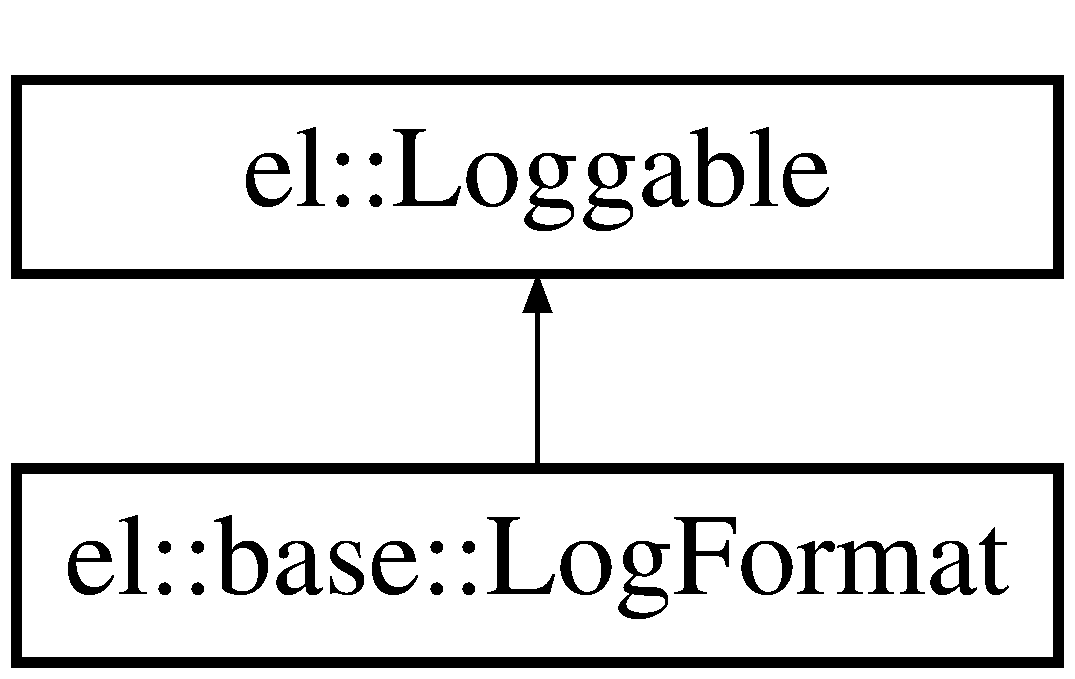
\includegraphics[height=2.000000cm]{classel_1_1base_1_1LogFormat}
\end{center}
\end{figure}
\subsection*{Public Member Functions}
\begin{DoxyCompactItemize}
\item 
\hypertarget{classel_1_1base_1_1LogFormat_a746a49231f1b046803dd2144ae2a2c76}{{\bfseries Log\-Format} (\hyperlink{namespaceel_ab0ac6091262344c52dd2d3ad099e8e36}{Level} level, const base\-::type\-::string\-\_\-t \&format)}\label{classel_1_1base_1_1LogFormat_a746a49231f1b046803dd2144ae2a2c76}

\item 
\hypertarget{classel_1_1base_1_1LogFormat_a8cc88ab095024bcfb90dd3ad7208f2ef}{{\bfseries Log\-Format} (const \hyperlink{classel_1_1base_1_1LogFormat}{Log\-Format} \&log\-Format)}\label{classel_1_1base_1_1LogFormat_a8cc88ab095024bcfb90dd3ad7208f2ef}

\item 
\hypertarget{classel_1_1base_1_1LogFormat_a697d52d55c6b6c6b8e6d5ceb37d66c19}{{\bfseries Log\-Format} (\hyperlink{classel_1_1base_1_1LogFormat}{Log\-Format} \&\&log\-Format)}\label{classel_1_1base_1_1LogFormat_a697d52d55c6b6c6b8e6d5ceb37d66c19}

\item 
\hypertarget{classel_1_1base_1_1LogFormat_a3c81e5976c3f3a8cb428eeeb3f188ac2}{\hyperlink{classel_1_1base_1_1LogFormat}{Log\-Format} \& {\bfseries operator=} (const \hyperlink{classel_1_1base_1_1LogFormat}{Log\-Format} \&log\-Format)}\label{classel_1_1base_1_1LogFormat_a3c81e5976c3f3a8cb428eeeb3f188ac2}

\item 
\hypertarget{classel_1_1base_1_1LogFormat_a31e85c6f74da6fe36d156a89a6c7fb91}{bool {\bfseries operator==} (const \hyperlink{classel_1_1base_1_1LogFormat}{Log\-Format} \&other)}\label{classel_1_1base_1_1LogFormat_a31e85c6f74da6fe36d156a89a6c7fb91}

\item 
void \hyperlink{classel_1_1base_1_1LogFormat_ab7c1b15cfdad24cfbc6dbced8b9d66eb}{parse\-From\-Format} (const base\-::type\-::string\-\_\-t \&user\-Format)
\begin{DoxyCompactList}\small\item\em Updates format to be used while logging. \end{DoxyCompactList}\item 
\hypertarget{classel_1_1base_1_1LogFormat_a6c5d17ad378ccb6e53beb2d48143fecb}{\hyperlink{namespaceel_ab0ac6091262344c52dd2d3ad099e8e36}{Level} {\bfseries level} (void) const }\label{classel_1_1base_1_1LogFormat_a6c5d17ad378ccb6e53beb2d48143fecb}

\item 
\hypertarget{classel_1_1base_1_1LogFormat_a9ca6ecd5b9342653493670d5a4e230cd}{const base\-::type\-::string\-\_\-t \& {\bfseries user\-Format} (void) const }\label{classel_1_1base_1_1LogFormat_a9ca6ecd5b9342653493670d5a4e230cd}

\item 
\hypertarget{classel_1_1base_1_1LogFormat_ac19602b3153daa9a76b56d3f4ff3beaa}{const base\-::type\-::string\-\_\-t \& {\bfseries format} (void) const }\label{classel_1_1base_1_1LogFormat_ac19602b3153daa9a76b56d3f4ff3beaa}

\item 
\hypertarget{classel_1_1base_1_1LogFormat_aa06b2643592f8a441d93cde673640262}{const std\-::string \& {\bfseries date\-Time\-Format} (void) const }\label{classel_1_1base_1_1LogFormat_aa06b2643592f8a441d93cde673640262}

\item 
\hypertarget{classel_1_1base_1_1LogFormat_a3ecf5f8df9b9e090784e19ad76046c49}{base\-::type\-::\-Enum\-Type {\bfseries flags} (void) const }\label{classel_1_1base_1_1LogFormat_a3ecf5f8df9b9e090784e19ad76046c49}

\item 
\hypertarget{classel_1_1base_1_1LogFormat_ae3634f9d90f7339d99eec8512b46c734}{bool {\bfseries has\-Flag} (\hyperlink{namespaceel_1_1base_a28939c5a884e67fcf12259f4b8848e00}{base\-::\-Format\-Flags} flag) const }\label{classel_1_1base_1_1LogFormat_ae3634f9d90f7339d99eec8512b46c734}

\item 
\hypertarget{classel_1_1base_1_1LogFormat_a0cae595d1a367538243feb1be1555d2e}{virtual void {\bfseries log} (el\-::base\-::type\-::ostream\-\_\-t \&os) const }\label{classel_1_1base_1_1LogFormat_a0cae595d1a367538243feb1be1555d2e}

\end{DoxyCompactItemize}
\subsection*{Protected Member Functions}
\begin{DoxyCompactItemize}
\item 
virtual void \hyperlink{classel_1_1base_1_1LogFormat_a3146651eadd6b1164bde74e5b273ec94}{update\-Date\-Format} (std\-::size\-\_\-t index, base\-::type\-::string\-\_\-t \&curr\-Format) E\-L\-P\-P\-\_\-\-F\-I\-N\-A\-L
\begin{DoxyCompactList}\small\item\em Updates date time format if available in curr\-Format. \end{DoxyCompactList}\item 
\hypertarget{classel_1_1base_1_1LogFormat_afee2335cce2b627dfd7f918d5a2b85f3}{virtual void \hyperlink{classel_1_1base_1_1LogFormat_afee2335cce2b627dfd7f918d5a2b85f3}{update\-Format\-Spec} (void) E\-L\-P\-P\-\_\-\-F\-I\-N\-A\-L}\label{classel_1_1base_1_1LogFormat_afee2335cce2b627dfd7f918d5a2b85f3}

\begin{DoxyCompactList}\small\item\em Updates level from format. This is so that we dont have to do it at log-\/writing-\/time. It uses m\-\_\-format and m\-\_\-level. \end{DoxyCompactList}\item 
\hypertarget{classel_1_1base_1_1LogFormat_ae55910f533a6eb3b41eb75b131e522bf}{void {\bfseries add\-Flag} (\hyperlink{namespaceel_1_1base_a28939c5a884e67fcf12259f4b8848e00}{base\-::\-Format\-Flags} flag)}\label{classel_1_1base_1_1LogFormat_ae55910f533a6eb3b41eb75b131e522bf}

\end{DoxyCompactItemize}
\subsection*{Friends}
\begin{DoxyCompactItemize}
\item 
\hypertarget{classel_1_1base_1_1LogFormat_aa78553f3fecc0d9551408dfd7aa7f737}{class {\bfseries el\-::\-Logger}}\label{classel_1_1base_1_1LogFormat_aa78553f3fecc0d9551408dfd7aa7f737}

\end{DoxyCompactItemize}


\subsection{Detailed Description}
Represents log format containing flags and date format. This is used internally to start initial log. 

\subsection{Member Function Documentation}
\hypertarget{classel_1_1base_1_1LogFormat_ab7c1b15cfdad24cfbc6dbced8b9d66eb}{\index{el\-::base\-::\-Log\-Format@{el\-::base\-::\-Log\-Format}!parse\-From\-Format@{parse\-From\-Format}}
\index{parse\-From\-Format@{parse\-From\-Format}!el::base::LogFormat@{el\-::base\-::\-Log\-Format}}
\subsubsection[{parse\-From\-Format}]{\setlength{\rightskip}{0pt plus 5cm}void el\-::base\-::\-Log\-Format\-::parse\-From\-Format (
\begin{DoxyParamCaption}
\item[{const base\-::type\-::string\-\_\-t \&}]{user\-Format}
\end{DoxyParamCaption}
)\hspace{0.3cm}{\ttfamily [inline]}}}\label{classel_1_1base_1_1LogFormat_ab7c1b15cfdad24cfbc6dbced8b9d66eb}


Updates format to be used while logging. 


\begin{DoxyParams}{Parameters}
{\em user\-Format} & User provided format \\
\hline
\end{DoxyParams}
\hypertarget{classel_1_1base_1_1LogFormat_a3146651eadd6b1164bde74e5b273ec94}{\index{el\-::base\-::\-Log\-Format@{el\-::base\-::\-Log\-Format}!update\-Date\-Format@{update\-Date\-Format}}
\index{update\-Date\-Format@{update\-Date\-Format}!el::base::LogFormat@{el\-::base\-::\-Log\-Format}}
\subsubsection[{update\-Date\-Format}]{\setlength{\rightskip}{0pt plus 5cm}virtual void el\-::base\-::\-Log\-Format\-::update\-Date\-Format (
\begin{DoxyParamCaption}
\item[{std\-::size\-\_\-t}]{index, }
\item[{base\-::type\-::string\-\_\-t \&}]{curr\-Format}
\end{DoxyParamCaption}
)\hspace{0.3cm}{\ttfamily [inline]}, {\ttfamily [protected]}, {\ttfamily [virtual]}}}\label{classel_1_1base_1_1LogFormat_a3146651eadd6b1164bde74e5b273ec94}


Updates date time format if available in curr\-Format. 


\begin{DoxyParams}[1]{Parameters}
 & {\em index} & Index where datetime, date or time was found \\
\hline
\mbox{\tt in,out}  & {\em curr\-Format} & current format that is being used to format \\
\hline
\end{DoxyParams}


The documentation for this class was generated from the following file\-:\begin{DoxyCompactItemize}
\item 
include/sma/io/detail/logimpl.\-hpp\end{DoxyCompactItemize}

\hypertarget{classel_1_1Loggable}{\section{el\-:\-:Loggable Class Reference}
\label{classel_1_1Loggable}\index{el\-::\-Loggable@{el\-::\-Loggable}}
}


Base of Easylogging++ friendly class.  




{\ttfamily \#include $<$logimpl.\-hpp$>$}

Inheritance diagram for el\-:\-:Loggable\-:\begin{figure}[H]
\begin{center}
\leavevmode
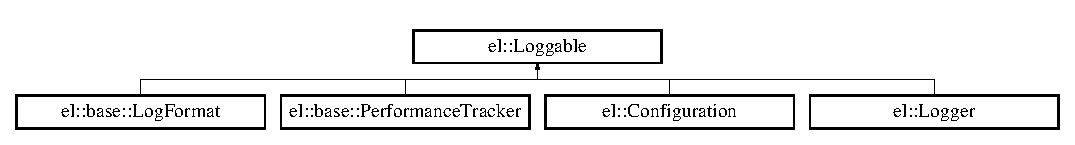
\includegraphics[height=1.505376cm]{classel_1_1Loggable}
\end{center}
\end{figure}
\subsection*{Public Member Functions}
\begin{DoxyCompactItemize}
\item 
\hypertarget{classel_1_1Loggable_ad8a2e0ebc11e4bd00ef49fc67db3d59e}{virtual void {\bfseries log} (el\-::base\-::type\-::ostream\-\_\-t \&) const =0}\label{classel_1_1Loggable_ad8a2e0ebc11e4bd00ef49fc67db3d59e}

\end{DoxyCompactItemize}
\subsection*{Friends}
\begin{DoxyCompactItemize}
\item 
\hypertarget{classel_1_1Loggable_a00722a386f498be3ebece2e266fb0f05}{el\-::base\-::type\-::ostream\-\_\-t \& {\bfseries operator$<$$<$} (el\-::base\-::type\-::ostream\-\_\-t \&os, const \hyperlink{classel_1_1Loggable}{Loggable} \&loggable)}\label{classel_1_1Loggable_a00722a386f498be3ebece2e266fb0f05}

\end{DoxyCompactItemize}


\subsection{Detailed Description}
Base of Easylogging++ friendly class. 

After inheriting this class publicly, implement pure-\/virtual function {\ttfamily void log(std\-::ostream\&) const} 

The documentation for this class was generated from the following file\-:\begin{DoxyCompactItemize}
\item 
include/sma/io/detail/logimpl.\-hpp\end{DoxyCompactItemize}

\hypertarget{structsma_1_1Logger}{\section{sma\-:\-:Logger Struct Reference}
\label{structsma_1_1Logger}\index{sma\-::\-Logger@{sma\-::\-Logger}}
}
\subsection*{Public Member Functions}
\begin{DoxyCompactItemize}
\item 
\hypertarget{structsma_1_1Logger_aa3adf99841d56561e64dc7feb77d4e78}{{\bfseries Logger} (std\-::string id)}\label{structsma_1_1Logger_aa3adf99841d56561e64dc7feb77d4e78}

\item 
\hypertarget{structsma_1_1Logger_abb1b7810f6a3049162b330fbbcc77a44}{{\footnotesize template$<$typename... Args$>$ }\\\hyperlink{structsma_1_1Logger}{Logger} const \& {\bfseries t} (Args \&\&...args) const }\label{structsma_1_1Logger_abb1b7810f6a3049162b330fbbcc77a44}

\item 
\hypertarget{structsma_1_1Logger_a3ed4dcc5f23e11bc92ddc6b3abebf4f4}{{\footnotesize template$<$typename... Args$>$ }\\\hyperlink{structsma_1_1Logger}{Logger} const \& {\bfseries d} (Args \&\&...args) const }\label{structsma_1_1Logger_a3ed4dcc5f23e11bc92ddc6b3abebf4f4}

\item 
\hypertarget{structsma_1_1Logger_acbe6362c4d08b6da868ff5b55b255201}{{\footnotesize template$<$typename... Args$>$ }\\\hyperlink{structsma_1_1Logger}{Logger} const \& {\bfseries i} (Args \&\&...args) const }\label{structsma_1_1Logger_acbe6362c4d08b6da868ff5b55b255201}

\item 
\hypertarget{structsma_1_1Logger_a6da957582bb2e7752c55677330ce6944}{{\footnotesize template$<$typename... Args$>$ }\\\hyperlink{structsma_1_1Logger}{Logger} const \& {\bfseries w} (Args \&\&...args) const }\label{structsma_1_1Logger_a6da957582bb2e7752c55677330ce6944}

\item 
\hypertarget{structsma_1_1Logger_ab21f9f52bb22c0df8f943b5774fc7be7}{{\footnotesize template$<$typename... Args$>$ }\\\hyperlink{structsma_1_1Logger}{Logger} const \& {\bfseries e} (Args \&\&...args) const }\label{structsma_1_1Logger_ab21f9f52bb22c0df8f943b5774fc7be7}

\item 
\hypertarget{structsma_1_1Logger_a43d1684ce6e1e3ec15cbd93f285368fe}{{\footnotesize template$<$typename... Args$>$ }\\\hyperlink{structsma_1_1Logger}{Logger} const \& {\bfseries f} (Args \&\&...args) const }\label{structsma_1_1Logger_a43d1684ce6e1e3ec15cbd93f285368fe}

\end{DoxyCompactItemize}


The documentation for this struct was generated from the following file\-:\begin{DoxyCompactItemize}
\item 
include/sma/io/log.\-hpp\end{DoxyCompactItemize}

\hypertarget{classel_1_1Logger}{\section{el\-:\-:Logger Class Reference}
\label{classel_1_1Logger}\index{el\-::\-Logger@{el\-::\-Logger}}
}


Represents a logger holding I\-D and configurations we need to write logs.  




{\ttfamily \#include $<$logimpl.\-hpp$>$}

Inheritance diagram for el\-:\-:Logger\-:\begin{figure}[H]
\begin{center}
\leavevmode
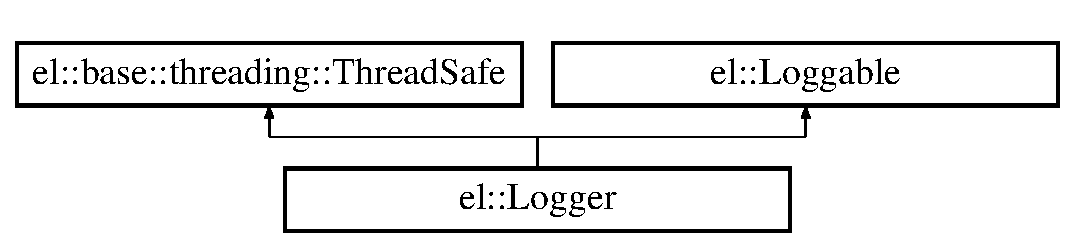
\includegraphics[height=2.000000cm]{classel_1_1Logger}
\end{center}
\end{figure}
\subsection*{Public Member Functions}
\begin{DoxyCompactItemize}
\item 
\hypertarget{classel_1_1Logger_a59b1c5a0f8c5c670e59d2f69f9e39fbb}{{\bfseries Logger} (const std\-::string \&id, base\-::\-Log\-Streams\-Reference\-Map $\ast$log\-Streams\-Reference)}\label{classel_1_1Logger_a59b1c5a0f8c5c670e59d2f69f9e39fbb}

\item 
\hypertarget{classel_1_1Logger_a43abea8865d7316f05c8a676a8c04896}{{\bfseries Logger} (const std\-::string \&id, const \hyperlink{classel_1_1Configurations}{Configurations} \&configurations, base\-::\-Log\-Streams\-Reference\-Map $\ast$log\-Streams\-Reference)}\label{classel_1_1Logger_a43abea8865d7316f05c8a676a8c04896}

\item 
\hypertarget{classel_1_1Logger_a984de07936a8c783e91496dfa6df69ea}{{\bfseries Logger} (const \hyperlink{classel_1_1Logger}{Logger} \&logger)}\label{classel_1_1Logger_a984de07936a8c783e91496dfa6df69ea}

\item 
\hypertarget{classel_1_1Logger_a2bfb4ed37f3281a701f20fb21a4cac62}{\hyperlink{classel_1_1Logger}{Logger} \& {\bfseries operator=} (const \hyperlink{classel_1_1Logger}{Logger} \&logger)}\label{classel_1_1Logger_a2bfb4ed37f3281a701f20fb21a4cac62}

\item 
\hypertarget{classel_1_1Logger_a12e1e5f6f91bad8d6a71c3918f09b672}{virtual void {\bfseries log} (el\-::base\-::type\-::ostream\-\_\-t \&os) const }\label{classel_1_1Logger_a12e1e5f6f91bad8d6a71c3918f09b672}

\item 
\hypertarget{classel_1_1Logger_ad9db621dbf8977bf814dc7baea8dcee4}{void \hyperlink{classel_1_1Logger_ad9db621dbf8977bf814dc7baea8dcee4}{configure} (const \hyperlink{classel_1_1Configurations}{Configurations} \&configurations)}\label{classel_1_1Logger_ad9db621dbf8977bf814dc7baea8dcee4}

\begin{DoxyCompactList}\small\item\em Configures the logger using specified configurations. \end{DoxyCompactList}\item 
\hypertarget{classel_1_1Logger_adfd57ab27fb398cc980a3edfab92927e}{void \hyperlink{classel_1_1Logger_adfd57ab27fb398cc980a3edfab92927e}{reconfigure} (void)}\label{classel_1_1Logger_adfd57ab27fb398cc980a3edfab92927e}

\begin{DoxyCompactList}\small\item\em Reconfigures logger using existing configurations. \end{DoxyCompactList}\item 
\hypertarget{classel_1_1Logger_ae51a621df3c835f51f450134ba66f8ac}{const std\-::string \& {\bfseries id} (void) const }\label{classel_1_1Logger_ae51a621df3c835f51f450134ba66f8ac}

\item 
\hypertarget{classel_1_1Logger_a9e56e468bccd7b52281e7bbc75892431}{const std\-::string \& {\bfseries parent\-Application\-Name} (void) const }\label{classel_1_1Logger_a9e56e468bccd7b52281e7bbc75892431}

\item 
\hypertarget{classel_1_1Logger_a6890af8910adba26b01ef029429c4f15}{void {\bfseries set\-Parent\-Application\-Name} (const std\-::string \&parent\-Application\-Name)}\label{classel_1_1Logger_a6890af8910adba26b01ef029429c4f15}

\item 
\hypertarget{classel_1_1Logger_aeb57aeaddbb3dcd0cb96114019817142}{\hyperlink{classel_1_1Configurations}{Configurations} $\ast$ {\bfseries configurations} (void)}\label{classel_1_1Logger_aeb57aeaddbb3dcd0cb96114019817142}

\item 
\hypertarget{classel_1_1Logger_ac1d34e77892ea506b011d5279b6b139d}{\hyperlink{classel_1_1base_1_1TypedConfigurations}{base\-::\-Typed\-Configurations} $\ast$ {\bfseries typed\-Configurations} (void)}\label{classel_1_1Logger_ac1d34e77892ea506b011d5279b6b139d}

\item 
\hypertarget{classel_1_1Logger_a9a89d454008b1ee1a197eec4b92ce22a}{void \hyperlink{classel_1_1Logger_a9a89d454008b1ee1a197eec4b92ce22a}{flush} (void)}\label{classel_1_1Logger_a9a89d454008b1ee1a197eec4b92ce22a}

\begin{DoxyCompactList}\small\item\em Flushes logger to sync all log files for all levels. \end{DoxyCompactList}\item 
\hypertarget{classel_1_1Logger_aead5b130c5141d2024740b03ab4b45d7}{\hyperlink{classel_1_1LogBuilder}{Log\-Builder} $\ast$ {\bfseries log\-Builder} (void) const }\label{classel_1_1Logger_aead5b130c5141d2024740b03ab4b45d7}

\item 
\hypertarget{classel_1_1Logger_a737340322cc9d9d20febd7131c1e262f}{void {\bfseries set\-Log\-Builder} (const Log\-Builder\-Ptr \&log\-Builder)}\label{classel_1_1Logger_a737340322cc9d9d20febd7131c1e262f}

\item 
\hypertarget{classel_1_1Logger_a5abaca24ac28bfd4806bea32be193435}{bool {\bfseries enabled} (\hyperlink{namespaceel_ab0ac6091262344c52dd2d3ad099e8e36}{Level} level) const }\label{classel_1_1Logger_a5abaca24ac28bfd4806bea32be193435}

\end{DoxyCompactItemize}
\subsection*{Static Public Member Functions}
\begin{DoxyCompactItemize}
\item 
\hypertarget{classel_1_1Logger_af6cf4f266ceb65da9563afd3706f26d6}{static bool {\bfseries is\-Valid\-Id} (const std\-::string \&id)}\label{classel_1_1Logger_af6cf4f266ceb65da9563afd3706f26d6}

\end{DoxyCompactItemize}
\subsection*{Friends}
\begin{DoxyCompactItemize}
\item 
\hypertarget{classel_1_1Logger_a22965b691242a9f61d443ba03fce3e35}{class {\bfseries el\-::\-Log\-Message}}\label{classel_1_1Logger_a22965b691242a9f61d443ba03fce3e35}

\item 
\hypertarget{classel_1_1Logger_a6efe246b312d02731fb0e1d120c0331d}{class {\bfseries el\-::\-Loggers}}\label{classel_1_1Logger_a6efe246b312d02731fb0e1d120c0331d}

\item 
\hypertarget{classel_1_1Logger_a2fb8a2c02cbf86247f093c118bed877a}{class {\bfseries el\-::\-Helpers}}\label{classel_1_1Logger_a2fb8a2c02cbf86247f093c118bed877a}

\item 
\hypertarget{classel_1_1Logger_a574ecee25e8d578f76060a95a2fe7c9e}{class {\bfseries el\-::base\-::\-Registered\-Loggers}}\label{classel_1_1Logger_a574ecee25e8d578f76060a95a2fe7c9e}

\item 
\hypertarget{classel_1_1Logger_a42b1de96d584ae4fecbfc2b9aff95052}{class {\bfseries el\-::base\-::\-Default\-Log\-Dispatch\-Callback}}\label{classel_1_1Logger_a42b1de96d584ae4fecbfc2b9aff95052}

\item 
\hypertarget{classel_1_1Logger_a81bbf6fe31fab133d182efa8367304f1}{class {\bfseries el\-::base\-::\-Message\-Builder}}\label{classel_1_1Logger_a81bbf6fe31fab133d182efa8367304f1}

\item 
\hypertarget{classel_1_1Logger_a7a728edbb2761d151832daa74d5b2736}{class {\bfseries el\-::base\-::\-Writer}}\label{classel_1_1Logger_a7a728edbb2761d151832daa74d5b2736}

\item 
\hypertarget{classel_1_1Logger_a2a368b9be1b8d6a29d4bb92a11807f39}{class {\bfseries el\-::base\-::\-P\-Error\-Writer}}\label{classel_1_1Logger_a2a368b9be1b8d6a29d4bb92a11807f39}

\item 
\hypertarget{classel_1_1Logger_acc1efd1b8a3fc5e0028dab98b02e550a}{class {\bfseries el\-::base\-::\-Storage}}\label{classel_1_1Logger_acc1efd1b8a3fc5e0028dab98b02e550a}

\item 
\hypertarget{classel_1_1Logger_a6a4d7851e1984800be3c230f06a79528}{class {\bfseries el\-::base\-::\-Performance\-Tracker}}\label{classel_1_1Logger_a6a4d7851e1984800be3c230f06a79528}

\item 
\hypertarget{classel_1_1Logger_a9b37b28ea1c5f8f862cc89f135711d92}{class {\bfseries el\-::base\-::\-Log\-Dispatcher}}\label{classel_1_1Logger_a9b37b28ea1c5f8f862cc89f135711d92}

\end{DoxyCompactItemize}


\subsection{Detailed Description}
Represents a logger holding I\-D and configurations we need to write logs. 

This class does not write logs itself instead its used by writer to read configuations from. 

The documentation for this class was generated from the following file\-:\begin{DoxyCompactItemize}
\item 
include/sma/io/detail/logimpl.\-hpp\end{DoxyCompactItemize}

\hypertarget{classel_1_1Loggers}{\section{el\-:\-:Loggers Class Reference}
\label{classel_1_1Loggers}\index{el\-::\-Loggers@{el\-::\-Loggers}}
}


Static helpers to deal with loggers and their configurations.  




{\ttfamily \#include $<$logimpl.\-hpp$>$}

Inheritance diagram for el\-:\-:Loggers\-:\begin{figure}[H]
\begin{center}
\leavevmode
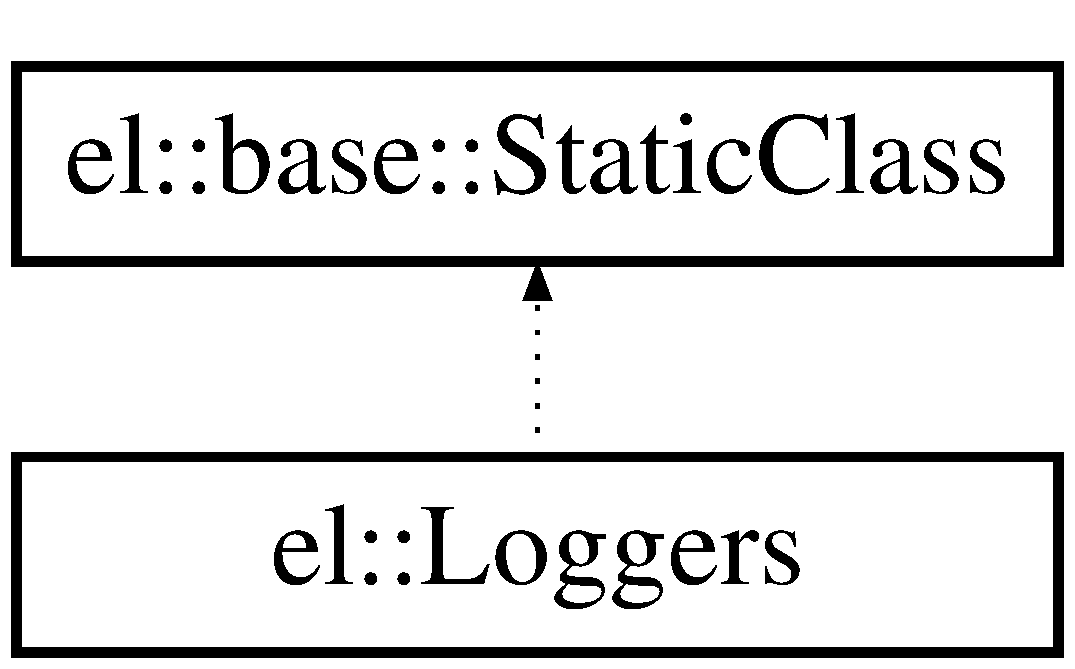
\includegraphics[height=2.000000cm]{classel_1_1Loggers}
\end{center}
\end{figure}
\subsection*{Classes}
\begin{DoxyCompactItemize}
\item 
class \hyperlink{classel_1_1Loggers_1_1ScopedAddFlag}{Scoped\-Add\-Flag}
\begin{DoxyCompactList}\small\item\em Adds flag and removes it when scope goes out. \end{DoxyCompactList}\item 
class \hyperlink{classel_1_1Loggers_1_1ScopedRemoveFlag}{Scoped\-Remove\-Flag}
\begin{DoxyCompactList}\small\item\em Removes flag and add it when scope goes out. \end{DoxyCompactList}\end{DoxyCompactItemize}
\subsection*{Static Public Member Functions}
\begin{DoxyCompactItemize}
\item 
\hypertarget{classel_1_1Loggers_aaebf868c558e3ba1d2e4f073a00f1d4a}{static \hyperlink{classel_1_1Logger}{Logger} $\ast$ \hyperlink{classel_1_1Loggers_aaebf868c558e3ba1d2e4f073a00f1d4a}{get\-Logger} (const std\-::string \&identity, bool register\-If\-Not\-Available=true)}\label{classel_1_1Loggers_aaebf868c558e3ba1d2e4f073a00f1d4a}

\begin{DoxyCompactList}\small\item\em Gets existing or registers new logger. \end{DoxyCompactList}\item 
\hypertarget{classel_1_1Loggers_a201d261ea57c070f07f0bf2006158587}{static bool \hyperlink{classel_1_1Loggers_a201d261ea57c070f07f0bf2006158587}{unregister\-Logger} (const std\-::string \&identity)}\label{classel_1_1Loggers_a201d261ea57c070f07f0bf2006158587}

\begin{DoxyCompactList}\small\item\em Unregisters logger -\/ use it only when you know what you are doing, you may unregister loggers initialized / used by third-\/party libs. \end{DoxyCompactList}\item 
\hypertarget{classel_1_1Loggers_a2d7a056cb7d9da3d96c709a2fac5c2bb}{static bool \hyperlink{classel_1_1Loggers_a2d7a056cb7d9da3d96c709a2fac5c2bb}{has\-Logger} (const std\-::string \&identity)}\label{classel_1_1Loggers_a2d7a056cb7d9da3d96c709a2fac5c2bb}

\begin{DoxyCompactList}\small\item\em Whether or not logger with id is registered. \end{DoxyCompactList}\item 
\hypertarget{classel_1_1Loggers_a888aca5bdccccc322da2eed430909d04}{static \hyperlink{classel_1_1Logger}{Logger} $\ast$ \hyperlink{classel_1_1Loggers_a888aca5bdccccc322da2eed430909d04}{reconfigure\-Logger} (\hyperlink{classel_1_1Logger}{Logger} $\ast$logger, const \hyperlink{classel_1_1Configurations}{Configurations} \&configurations)}\label{classel_1_1Loggers_a888aca5bdccccc322da2eed430909d04}

\begin{DoxyCompactList}\small\item\em Reconfigures specified logger with new configurations. \end{DoxyCompactList}\item 
\hypertarget{classel_1_1Loggers_a105f776fe19cb7fa2fccd2993d9f7a7c}{static \hyperlink{classel_1_1Logger}{Logger} $\ast$ \hyperlink{classel_1_1Loggers_a105f776fe19cb7fa2fccd2993d9f7a7c}{reconfigure\-Logger} (const std\-::string \&identity, const \hyperlink{classel_1_1Configurations}{Configurations} \&configurations)}\label{classel_1_1Loggers_a105f776fe19cb7fa2fccd2993d9f7a7c}

\begin{DoxyCompactList}\small\item\em Reconfigures logger with new configurations after looking it up using identity. \end{DoxyCompactList}\item 
\hypertarget{classel_1_1Loggers_aef49fdae329cefcc1c01428568dced4b}{static \hyperlink{classel_1_1Logger}{Logger} $\ast$ \hyperlink{classel_1_1Loggers_aef49fdae329cefcc1c01428568dced4b}{reconfigure\-Logger} (const std\-::string \&identity, \hyperlink{namespaceel_a281f5db6d6163678bc68a8b23b59e124}{Configuration\-Type} configuration\-Type, const std\-::string \&value)}\label{classel_1_1Loggers_aef49fdae329cefcc1c01428568dced4b}

\begin{DoxyCompactList}\small\item\em Reconfigures logger's single configuration. \end{DoxyCompactList}\item 
\hypertarget{classel_1_1Loggers_ac834df0f5e9e3dab18e70321a2543af7}{static void \hyperlink{classel_1_1Loggers_ac834df0f5e9e3dab18e70321a2543af7}{reconfigure\-All\-Loggers} (const \hyperlink{classel_1_1Configurations}{Configurations} \&configurations)}\label{classel_1_1Loggers_ac834df0f5e9e3dab18e70321a2543af7}

\begin{DoxyCompactList}\small\item\em Reconfigures all the existing loggers with new configurations. \end{DoxyCompactList}\item 
\hypertarget{classel_1_1Loggers_a1ebd33bc0208b430f41508e34509c7c9}{static void \hyperlink{classel_1_1Loggers_a1ebd33bc0208b430f41508e34509c7c9}{reconfigure\-All\-Loggers} (\hyperlink{namespaceel_a281f5db6d6163678bc68a8b23b59e124}{Configuration\-Type} configuration\-Type, const std\-::string \&value)}\label{classel_1_1Loggers_a1ebd33bc0208b430f41508e34509c7c9}

\begin{DoxyCompactList}\small\item\em Reconfigures single configuration for all the loggers. \end{DoxyCompactList}\item 
\hypertarget{classel_1_1Loggers_ab24b99e5bb3c907d1418ee3266f15397}{static void \hyperlink{classel_1_1Loggers_ab24b99e5bb3c907d1418ee3266f15397}{reconfigure\-All\-Loggers} (\hyperlink{namespaceel_ab0ac6091262344c52dd2d3ad099e8e36}{Level} level, \hyperlink{namespaceel_a281f5db6d6163678bc68a8b23b59e124}{Configuration\-Type} configuration\-Type, const std\-::string \&value)}\label{classel_1_1Loggers_ab24b99e5bb3c907d1418ee3266f15397}

\begin{DoxyCompactList}\small\item\em Reconfigures single configuration for all the loggers for specified level. \end{DoxyCompactList}\item 
\hypertarget{classel_1_1Loggers_ab9fb62a8ff904ff887fefde3282f46a4}{static void \hyperlink{classel_1_1Loggers_ab9fb62a8ff904ff887fefde3282f46a4}{set\-Default\-Configurations} (const \hyperlink{classel_1_1Configurations}{Configurations} \&configurations, bool reconfigure\-Existing\-Loggers=false)}\label{classel_1_1Loggers_ab9fb62a8ff904ff887fefde3282f46a4}

\begin{DoxyCompactList}\small\item\em Sets default configurations. This configuration is used for future (and conditionally for existing) loggers. \end{DoxyCompactList}\item 
\hypertarget{classel_1_1Loggers_a96f2336fafdc3ef2c4df01a73ae5ffb7}{static const \hyperlink{classel_1_1Configurations}{Configurations} $\ast$ \hyperlink{classel_1_1Loggers_a96f2336fafdc3ef2c4df01a73ae5ffb7}{default\-Configurations} (void)}\label{classel_1_1Loggers_a96f2336fafdc3ef2c4df01a73ae5ffb7}

\begin{DoxyCompactList}\small\item\em Returns current default. \end{DoxyCompactList}\item 
\hypertarget{classel_1_1Loggers_ad17312c9474d94bc98efcaf08ca279a4}{static const \\*
base\-::\-Log\-Streams\-Reference\-Map $\ast$ \hyperlink{classel_1_1Loggers_ad17312c9474d94bc98efcaf08ca279a4}{log\-Streams\-Reference} (void)}\label{classel_1_1Loggers_ad17312c9474d94bc98efcaf08ca279a4}

\begin{DoxyCompactList}\small\item\em Returns log stream reference pointer if needed by user. \end{DoxyCompactList}\item 
\hypertarget{classel_1_1Loggers_af296007c3eb3b71602ec80ff59875b46}{static \hyperlink{classel_1_1base_1_1TypedConfigurations}{base\-::\-Typed\-Configurations} \hyperlink{classel_1_1Loggers_af296007c3eb3b71602ec80ff59875b46}{default\-Typed\-Configurations} (void)}\label{classel_1_1Loggers_af296007c3eb3b71602ec80ff59875b46}

\begin{DoxyCompactList}\small\item\em Default typed configuration based on existing default\-Conf. \end{DoxyCompactList}\item 
static std\-::vector$<$ std\-::string $>$ $\ast$ \hyperlink{classel_1_1Loggers_adea07ec6cbc1dfc50f939d69dcac7160}{populate\-All\-Logger\-Ids} (std\-::vector$<$ std\-::string $>$ $\ast$target\-List)
\begin{DoxyCompactList}\small\item\em Populates all logger I\-Ds in current repository. \end{DoxyCompactList}\item 
\hypertarget{classel_1_1Loggers_a9992995a85745639aa9aa5a2df2255f5}{static void \hyperlink{classel_1_1Loggers_a9992995a85745639aa9aa5a2df2255f5}{configure\-From\-Global} (const char $\ast$global\-Configuration\-File\-Path)}\label{classel_1_1Loggers_a9992995a85745639aa9aa5a2df2255f5}

\begin{DoxyCompactList}\small\item\em Sets configurations from global configuration file. \end{DoxyCompactList}\item 
static bool \hyperlink{classel_1_1Loggers_a28acf6f2b1ea7e5edd1b2560cde82406}{configure\-From\-Arg} (const char $\ast$arg\-Key)
\begin{DoxyCompactList}\small\item\em Configures loggers using command line arg. Ensure you have already set command line args,. \end{DoxyCompactList}\item 
\hypertarget{classel_1_1Loggers_a1834480e970c16817459ca3ee26b44b5}{static void \hyperlink{classel_1_1Loggers_a1834480e970c16817459ca3ee26b44b5}{flush\-All} (void)}\label{classel_1_1Loggers_a1834480e970c16817459ca3ee26b44b5}

\begin{DoxyCompactList}\small\item\em Flushes all loggers for all levels -\/ Be careful if you dont know how many loggers are registered. \end{DoxyCompactList}\item 
\hypertarget{classel_1_1Loggers_aedd2de02dd701b0f20ddaa10f1f728f1}{static void \hyperlink{classel_1_1Loggers_aedd2de02dd701b0f20ddaa10f1f728f1}{add\-Flag} (\hyperlink{namespaceel_a2784aacd04cb7816ac1c0b20fcbf83cb}{Logging\-Flag} flag)}\label{classel_1_1Loggers_aedd2de02dd701b0f20ddaa10f1f728f1}

\begin{DoxyCompactList}\small\item\em Adds logging flag used internally. \end{DoxyCompactList}\item 
\hypertarget{classel_1_1Loggers_a23fcb4b492f70a34285c45c0b5e2e515}{static void \hyperlink{classel_1_1Loggers_a23fcb4b492f70a34285c45c0b5e2e515}{remove\-Flag} (\hyperlink{namespaceel_a2784aacd04cb7816ac1c0b20fcbf83cb}{Logging\-Flag} flag)}\label{classel_1_1Loggers_a23fcb4b492f70a34285c45c0b5e2e515}

\begin{DoxyCompactList}\small\item\em Removes logging flag used internally. \end{DoxyCompactList}\item 
\hypertarget{classel_1_1Loggers_a591a45565c1eb7073ec3a979df8b5a4c}{static bool \hyperlink{classel_1_1Loggers_a591a45565c1eb7073ec3a979df8b5a4c}{has\-Flag} (\hyperlink{namespaceel_a2784aacd04cb7816ac1c0b20fcbf83cb}{Logging\-Flag} flag)}\label{classel_1_1Loggers_a591a45565c1eb7073ec3a979df8b5a4c}

\begin{DoxyCompactList}\small\item\em Determines whether or not certain flag is active. \end{DoxyCompactList}\item 
\hypertarget{classel_1_1Loggers_afbee019d722fef5148d8355f45ba7993}{static void \hyperlink{classel_1_1Loggers_afbee019d722fef5148d8355f45ba7993}{set\-Logging\-Level} (\hyperlink{namespaceel_ab0ac6091262344c52dd2d3ad099e8e36}{Level} level)}\label{classel_1_1Loggers_afbee019d722fef5148d8355f45ba7993}

\begin{DoxyCompactList}\small\item\em Sets hierarchy for logging. Needs to enable logging flag (Hierarchical\-Logging) \end{DoxyCompactList}\end{DoxyCompactItemize}


\subsection{Detailed Description}
Static helpers to deal with loggers and their configurations. 

\subsection{Member Function Documentation}
\hypertarget{classel_1_1Loggers_a28acf6f2b1ea7e5edd1b2560cde82406}{\index{el\-::\-Loggers@{el\-::\-Loggers}!configure\-From\-Arg@{configure\-From\-Arg}}
\index{configure\-From\-Arg@{configure\-From\-Arg}!el::Loggers@{el\-::\-Loggers}}
\subsubsection[{configure\-From\-Arg}]{\setlength{\rightskip}{0pt plus 5cm}static bool el\-::\-Loggers\-::configure\-From\-Arg (
\begin{DoxyParamCaption}
\item[{const char $\ast$}]{arg\-Key}
\end{DoxyParamCaption}
)\hspace{0.3cm}{\ttfamily [inline]}, {\ttfamily [static]}}}\label{classel_1_1Loggers_a28acf6f2b1ea7e5edd1b2560cde82406}


Configures loggers using command line arg. Ensure you have already set command line args,. 

\begin{DoxyReturn}{Returns}
False if invalid argument or argument with no value provided, true if attempted to configure logger. If true is returned that does not mean it has been configured successfully, it only means that it has attempeted to configure logger using configuration file provided in argument 
\end{DoxyReturn}
\hypertarget{classel_1_1Loggers_adea07ec6cbc1dfc50f939d69dcac7160}{\index{el\-::\-Loggers@{el\-::\-Loggers}!populate\-All\-Logger\-Ids@{populate\-All\-Logger\-Ids}}
\index{populate\-All\-Logger\-Ids@{populate\-All\-Logger\-Ids}!el::Loggers@{el\-::\-Loggers}}
\subsubsection[{populate\-All\-Logger\-Ids}]{\setlength{\rightskip}{0pt plus 5cm}static std\-::vector$<$std\-::string$>$$\ast$ el\-::\-Loggers\-::populate\-All\-Logger\-Ids (
\begin{DoxyParamCaption}
\item[{std\-::vector$<$ std\-::string $>$ $\ast$}]{target\-List}
\end{DoxyParamCaption}
)\hspace{0.3cm}{\ttfamily [inline]}, {\ttfamily [static]}}}\label{classel_1_1Loggers_adea07ec6cbc1dfc50f939d69dcac7160}


Populates all logger I\-Ds in current repository. 


\begin{DoxyParams}[1]{Parameters}
\mbox{\tt out}  & {\em target\-List} & List of fill up. \\
\hline
\end{DoxyParams}


The documentation for this class was generated from the following file\-:\begin{DoxyCompactItemize}
\item 
include/sma/io/detail/logimpl.\-hpp\end{DoxyCompactItemize}

\hypertarget{classel_1_1LogMessage}{\section{el\-:\-:Log\-Message Class Reference}
\label{classel_1_1LogMessage}\index{el\-::\-Log\-Message@{el\-::\-Log\-Message}}
}
\subsection*{Public Member Functions}
\begin{DoxyCompactItemize}
\item 
\hypertarget{classel_1_1LogMessage_a6cb875167d28c57e11877f833d733e04}{{\bfseries Log\-Message} (\hyperlink{namespaceel_ab0ac6091262344c52dd2d3ad099e8e36}{Level} level, const std\-::string \&file, unsigned long int line, const std\-::string \&func, base\-::type\-::\-Verbose\-Level verbose\-Level, \hyperlink{classel_1_1Logger}{Logger} $\ast$logger)}\label{classel_1_1LogMessage_a6cb875167d28c57e11877f833d733e04}

\item 
\hypertarget{classel_1_1LogMessage_a09514a3bb7deae447c3141bc55b52d06}{\hyperlink{namespaceel_ab0ac6091262344c52dd2d3ad099e8e36}{Level} {\bfseries level} (void) const }\label{classel_1_1LogMessage_a09514a3bb7deae447c3141bc55b52d06}

\item 
\hypertarget{classel_1_1LogMessage_a8f72164d7bf31ea3b15a5c0201fca0c4}{const std\-::string \& {\bfseries file} (void) const }\label{classel_1_1LogMessage_a8f72164d7bf31ea3b15a5c0201fca0c4}

\item 
\hypertarget{classel_1_1LogMessage_a4bc97e6670d890cae719e3e9680b8373}{unsigned long int {\bfseries line} (void) const }\label{classel_1_1LogMessage_a4bc97e6670d890cae719e3e9680b8373}

\item 
\hypertarget{classel_1_1LogMessage_ae09cdff5620dcf8269b2b83bea722a2a}{const std\-::string \& {\bfseries func} (void) const }\label{classel_1_1LogMessage_ae09cdff5620dcf8269b2b83bea722a2a}

\item 
\hypertarget{classel_1_1LogMessage_a52e91b0dd3e5af96642622cc2a67aa88}{base\-::type\-::\-Verbose\-Level {\bfseries verbose\-Level} (void) const }\label{classel_1_1LogMessage_a52e91b0dd3e5af96642622cc2a67aa88}

\item 
\hypertarget{classel_1_1LogMessage_ae67b30a16a4115148ee32c9b2c91e03c}{\hyperlink{classel_1_1Logger}{Logger} $\ast$ {\bfseries logger} (void) const }\label{classel_1_1LogMessage_ae67b30a16a4115148ee32c9b2c91e03c}

\item 
\hypertarget{classel_1_1LogMessage_a0f34882ed8102061bb9bb247cb08a5c3}{const base\-::type\-::string\-\_\-t \& {\bfseries message} (void) const }\label{classel_1_1LogMessage_a0f34882ed8102061bb9bb247cb08a5c3}

\end{DoxyCompactItemize}


The documentation for this class was generated from the following file\-:\begin{DoxyCompactItemize}
\item 
include/sma/io/detail/logimpl.\-hpp\end{DoxyCompactItemize}

\hypertarget{classsma_1_1MemoryContentStore}{\section{sma\-:\-:Memory\-Content\-Store Class Reference}
\label{classsma_1_1MemoryContentStore}\index{sma\-::\-Memory\-Content\-Store@{sma\-::\-Memory\-Content\-Store}}
}
Inheritance diagram for sma\-:\-:Memory\-Content\-Store\-:\begin{figure}[H]
\begin{center}
\leavevmode
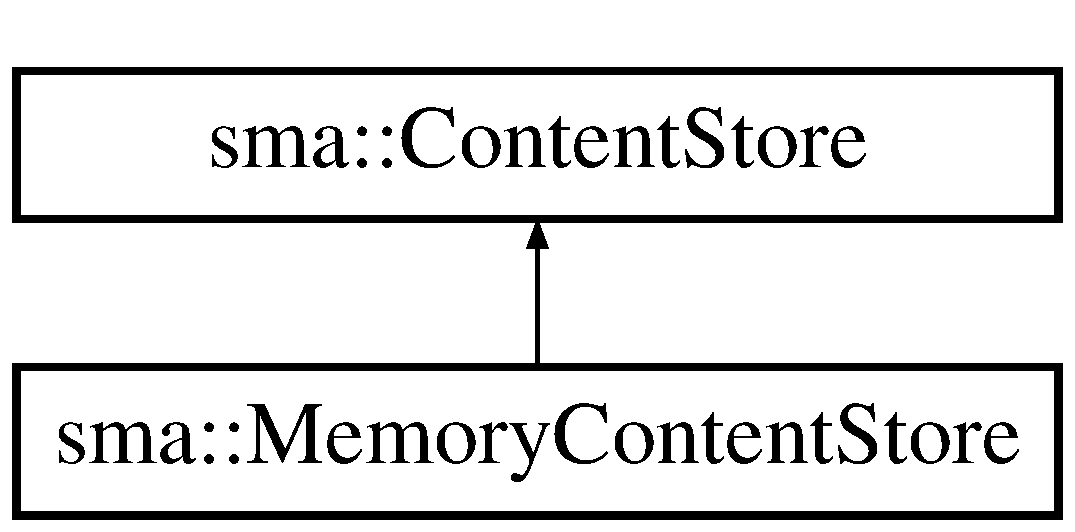
\includegraphics[height=2.000000cm]{classsma_1_1MemoryContentStore}
\end{center}
\end{figure}
\subsection*{Public Member Functions}
\begin{DoxyCompactItemize}
\item 
\hypertarget{classsma_1_1MemoryContentStore_ab8a9ffda41174ce2fda193dd91797d9f}{virtual Stored\-Content {\bfseries store} (std\-::istream \&is) override}\label{classsma_1_1MemoryContentStore_ab8a9ffda41174ce2fda193dd91797d9f}

\end{DoxyCompactItemize}


The documentation for this class was generated from the following file\-:\begin{DoxyCompactItemize}
\item 
include/sma/ccn/memorycontentstore.\-hpp\end{DoxyCompactItemize}

\hypertarget{structsma_1_1Message}{\section{sma\-:\-:Message Struct Reference}
\label{structsma_1_1Message}\index{sma\-::\-Message@{sma\-::\-Message}}
}
\subsection*{Public Member Functions}
\begin{DoxyCompactItemize}
\item 
\hypertarget{structsma_1_1Message_a65c46931c395532a94aa70894745f624}{{\footnotesize template$<$typename M $>$ }\\{\bfseries Message} (\hyperlink{structsma_1_1MessageHeader}{Message\-Header} header, M const \&msg)}\label{structsma_1_1Message_a65c46931c395532a94aa70894745f624}

\item 
\hypertarget{structsma_1_1Message_a47174b68653e8860dd2a6623dda3ef82}{std\-::uint8\-\_\-t const $\ast$ {\bfseries cdata} ()}\label{structsma_1_1Message_a47174b68653e8860dd2a6623dda3ef82}

\item 
\hypertarget{structsma_1_1Message_a47eda10f28a3804372f6a59847271c1a}{std\-::size\-\_\-t {\bfseries size} ()}\label{structsma_1_1Message_a47eda10f28a3804372f6a59847271c1a}

\end{DoxyCompactItemize}


The documentation for this struct was generated from the following file\-:\begin{DoxyCompactItemize}
\item 
include/sma/message.\-hpp\end{DoxyCompactItemize}

\hypertarget{classsma_1_1message__thread}{\section{sma\-:\-:message\-\_\-thread Class Reference}
\label{classsma_1_1message__thread}\index{sma\-::message\-\_\-thread@{sma\-::message\-\_\-thread}}
}


{\ttfamily \#include $<$message\-\_\-thread.\-hpp$>$}

\subsection*{Public Member Functions}
\begin{DoxyCompactItemize}
\item 
\hypertarget{classsma_1_1message__thread_ae2bf5e0973518dfffdd9832a9bd4296e}{const message \& {\bfseries cmsg} () const }\label{classsma_1_1message__thread_ae2bf5e0973518dfffdd9832a9bd4296e}

\end{DoxyCompactItemize}


\subsection{Detailed Description}
The message thread constantly tries to get a message from the assigned channel and dispatches it via the messenger's handler table. The thread loop therefore is\-:
\begin{DoxyEnumerate}
\item Lock channel
\item Wait until channel is not blocked
\item Check if any socket is ready for reading no\-: A. set blocked flag and enter select() wait B. go to 3 yes\-: A. remove one socket and unlock channel ---$>$ (another thread can now enter 1) B. read from socket into thread-\/local buffer C. parse header and go to msgr with dispatch info D. pick a handler or, if none, go to 1 E. execute handler and block F. return to 1 for a new message If handlers are reasonably short and message wait times are reasonably long then we could expect two threads to maximize usage as one is always blocked on reading while one is always executing a handler. If too many threads are in this loop then they'll contend over selecting a socket and locking the channel and it'll be worse than a smaller number of threads. Two is probably reasonable to maximize throughput.
\end{DoxyEnumerate}

The only thread-\/local state necessary is\-:
\begin{DoxyItemize}
\item the thread's read channel
\item the messenger with the handler dispatch table
\item the current message buffer, which lives for the duration of the handler. Letting the thread do the socket read into a field, and only guaranteeing its lifetime during the handler execution, means we can process messages concurrently with zero allocations. 
\end{DoxyItemize}

The documentation for this class was generated from the following file\-:\begin{DoxyCompactItemize}
\item 
android/core/include/sma/android/message\-\_\-thread.\-hpp\end{DoxyCompactItemize}

\hypertarget{classel_1_1base_1_1MessageBuilder}{\section{el\-:\-:base\-:\-:Message\-Builder Class Reference}
\label{classel_1_1base_1_1MessageBuilder}\index{el\-::base\-::\-Message\-Builder@{el\-::base\-::\-Message\-Builder}}
}
\subsection*{Public Member Functions}
\begin{DoxyCompactItemize}
\item 
\hypertarget{classel_1_1base_1_1MessageBuilder_a61729d9b620eb7b3e6ac1af69364553c}{void {\bfseries initialize} (\hyperlink{classel_1_1Logger}{Logger} $\ast$logger)}\label{classel_1_1base_1_1MessageBuilder_a61729d9b620eb7b3e6ac1af69364553c}

\item 
\hypertarget{classel_1_1base_1_1MessageBuilder_a740a968d7f2901d49a2e1c348cfea7bf}{\hyperlink{classel_1_1base_1_1MessageBuilder}{Message\-Builder} \& {\bfseries operator$<$$<$} (const std\-::string \&msg)}\label{classel_1_1base_1_1MessageBuilder_a740a968d7f2901d49a2e1c348cfea7bf}

\item 
\hypertarget{classel_1_1base_1_1MessageBuilder_a3397469a83257b3580624bdfbd9d7ac7}{{\bfseries E\-L\-P\-P\-\_\-\-S\-I\-M\-P\-L\-E\-\_\-\-L\-O\-G} (signed short) E\-L\-P\-P\-\_\-\-S\-I\-M\-P\-L\-E\-\_\-\-L\-O\-G(unsigned short) inline \hyperlink{classel_1_1base_1_1MessageBuilder}{Message\-Builder} \&operator$<$$<$(const std}\label{classel_1_1base_1_1MessageBuilder_a3397469a83257b3580624bdfbd9d7ac7}

\item 
\hypertarget{classel_1_1base_1_1MessageBuilder_a42c2a21a6bebb2ad52d22da054cd8f49}{\hyperlink{classel_1_1base_1_1MessageBuilder}{Message\-Builder} \& {\bfseries operator$<$$<$} (const wchar\-\_\-t $\ast$msg)}\label{classel_1_1base_1_1MessageBuilder_a42c2a21a6bebb2ad52d22da054cd8f49}

\item 
\hypertarget{classel_1_1base_1_1MessageBuilder_a884b9fd5f742f5fa25bbc78d3415a674}{\hyperlink{classel_1_1base_1_1MessageBuilder}{Message\-Builder} \& {\bfseries operator$<$$<$} (std\-::ostream \&($\ast$O\-Stream\-Mani)(std\-::ostream \&))}\label{classel_1_1base_1_1MessageBuilder_a884b9fd5f742f5fa25bbc78d3415a674}

\end{DoxyCompactItemize}


The documentation for this class was generated from the following file\-:\begin{DoxyCompactItemize}
\item 
include/sma/io/detail/logimpl.\-hpp\end{DoxyCompactItemize}

\hypertarget{structsma_1_1detail_1_1MessageData}{\section{sma\-:\-:detail\-:\-:Message\-Data Struct Reference}
\label{structsma_1_1detail_1_1MessageData}\index{sma\-::detail\-::\-Message\-Data@{sma\-::detail\-::\-Message\-Data}}
}


Represents one buffered serialized message.  




{\ttfamily \#include $<$linklayerimpl.\-hpp$>$}

\subsection*{Public Member Functions}
\begin{DoxyCompactItemize}
\item 
\hypertarget{structsma_1_1detail_1_1MessageData_a7003684bd71006bc579b40f179523af5}{{\bfseries Message\-Data} (\hyperlink{structsma_1_1detail_1_1MessageData}{Message\-Data} \&\&)=delete}\label{structsma_1_1detail_1_1MessageData_a7003684bd71006bc579b40f179523af5}

\item 
\hypertarget{structsma_1_1detail_1_1MessageData_acfaf2e1e04388a7a1bee38afe2fd60ce}{{\bfseries Message\-Data} (\hyperlink{structsma_1_1detail_1_1MessageData}{Message\-Data} const \&)=delete}\label{structsma_1_1detail_1_1MessageData_acfaf2e1e04388a7a1bee38afe2fd60ce}

\item 
\hypertarget{structsma_1_1detail_1_1MessageData_acd8dcc80646958508c6801231c8da4e2}{\hyperlink{structsma_1_1detail_1_1MessageData}{Message\-Data} \& {\bfseries operator=} (\hyperlink{structsma_1_1detail_1_1MessageData}{Message\-Data} \&\&)=delete}\label{structsma_1_1detail_1_1MessageData_acd8dcc80646958508c6801231c8da4e2}

\item 
\hypertarget{structsma_1_1detail_1_1MessageData_a234011c43f7b0556c809e1a759abf989}{\hyperlink{structsma_1_1detail_1_1MessageData}{Message\-Data} \& {\bfseries operator=} (\hyperlink{structsma_1_1detail_1_1MessageData}{Message\-Data} const \&)=delete}\label{structsma_1_1detail_1_1MessageData_a234011c43f7b0556c809e1a759abf989}

\end{DoxyCompactItemize}
\subsection*{Public Attributes}
\begin{DoxyCompactItemize}
\item 
\hypertarget{structsma_1_1detail_1_1MessageData_abec85f24802bce558f1da8b8175d4762}{char {\bfseries data} \mbox{[}8192\mbox{]}}\label{structsma_1_1detail_1_1MessageData_abec85f24802bce558f1da8b8175d4762}

\item 
\hypertarget{structsma_1_1detail_1_1MessageData_a09a8c912128079d92de8e0d587c448e5}{std\-::size\-\_\-t {\bfseries size}}\label{structsma_1_1detail_1_1MessageData_a09a8c912128079d92de8e0d587c448e5}

\end{DoxyCompactItemize}


\subsection{Detailed Description}
Represents one buffered serialized message. 

These are meant to be modified in-\/place by claiming one from the buffer and populating it. 

The documentation for this struct was generated from the following file\-:\begin{DoxyCompactItemize}
\item 
include/sma/linklayerimpl.\-hpp\end{DoxyCompactItemize}

\hypertarget{structsma_1_1MessageHeader}{\section{sma\-:\-:Message\-Header Struct Reference}
\label{structsma_1_1MessageHeader}\index{sma\-::\-Message\-Header@{sma\-::\-Message\-Header}}
}
\subsection*{Public Member Functions}
\begin{DoxyCompactItemize}
\item 
\hypertarget{structsma_1_1MessageHeader_a068a0443fb72b642ced89f3b6fd18f75}{{\bfseries Message\-Header} (\hyperlink{structsma_1_1NodeId}{Node\-Id} sender)}\label{structsma_1_1MessageHeader_a068a0443fb72b642ced89f3b6fd18f75}

\item 
\hypertarget{structsma_1_1MessageHeader_a9c84bb0cca03de103f1ac8142aa8460b}{{\bfseries Message\-Header} (\hyperlink{structsma_1_1NodeId}{Node\-Id} sender, std\-::vector$<$ \hyperlink{structsma_1_1NodeId}{Node\-Id} $>$ recipients)}\label{structsma_1_1MessageHeader_a9c84bb0cca03de103f1ac8142aa8460b}

\end{DoxyCompactItemize}
\subsection*{Public Attributes}
\begin{DoxyCompactItemize}
\item 
\hypertarget{structsma_1_1MessageHeader_a7f551459bb6ade786bb9dbab8a8655f9}{\hyperlink{structsma_1_1NodeId}{Node\-Id} {\bfseries sender}}\label{structsma_1_1MessageHeader_a7f551459bb6ade786bb9dbab8a8655f9}

\item 
\hypertarget{structsma_1_1MessageHeader_a5588c5e7f480ba8842e6ce7fcf4b8529}{std\-::vector$<$ \hyperlink{structsma_1_1NodeId}{Node\-Id} $>$ {\bfseries recipients}}\label{structsma_1_1MessageHeader_a5588c5e7f480ba8842e6ce7fcf4b8529}

\end{DoxyCompactItemize}


The documentation for this struct was generated from the following file\-:\begin{DoxyCompactItemize}
\item 
include/sma/messageheader.\-hpp\end{DoxyCompactItemize}

\hypertarget{classel_1_1base_1_1MillisecondsWidth}{\section{el\-:\-:base\-:\-:Milliseconds\-Width Class Reference}
\label{classel_1_1base_1_1MillisecondsWidth}\index{el\-::base\-::\-Milliseconds\-Width@{el\-::base\-::\-Milliseconds\-Width}}
}


A milliseconds width class containing actual width and offset for date/time.  




{\ttfamily \#include $<$logimpl.\-hpp$>$}

\subsection*{Public Member Functions}
\begin{DoxyCompactItemize}
\item 
\hypertarget{classel_1_1base_1_1MillisecondsWidth_a358fa0fcdd4076c4038ecdfc206de38a}{{\bfseries Milliseconds\-Width} (int width)}\label{classel_1_1base_1_1MillisecondsWidth_a358fa0fcdd4076c4038ecdfc206de38a}

\item 
\hypertarget{classel_1_1base_1_1MillisecondsWidth_a60f5fb6e31216d1268585b98d20517ff}{bool {\bfseries operator==} (const \hyperlink{classel_1_1base_1_1MillisecondsWidth}{Milliseconds\-Width} \&ms\-Width)}\label{classel_1_1base_1_1MillisecondsWidth_a60f5fb6e31216d1268585b98d20517ff}

\end{DoxyCompactItemize}
\subsection*{Public Attributes}
\begin{DoxyCompactItemize}
\item 
\hypertarget{classel_1_1base_1_1MillisecondsWidth_a31c468b0323d376505c4975720c7b66e}{int {\bfseries m\-\_\-width}}\label{classel_1_1base_1_1MillisecondsWidth_a31c468b0323d376505c4975720c7b66e}

\item 
\hypertarget{classel_1_1base_1_1MillisecondsWidth_a0e98edbecf602a915d4d609747c52669}{unsigned int {\bfseries m\-\_\-offset}}\label{classel_1_1base_1_1MillisecondsWidth_a0e98edbecf602a915d4d609747c52669}

\end{DoxyCompactItemize}


\subsection{Detailed Description}
A milliseconds width class containing actual width and offset for date/time. 

The documentation for this class was generated from the following file\-:\begin{DoxyCompactItemize}
\item 
include/sma/io/detail/logimpl.\-hpp\end{DoxyCompactItemize}

\hypertarget{classsma_1_1NativeChannel}{\section{sma\-:\-:Native\-Channel Class Reference}
\label{classsma_1_1NativeChannel}\index{sma\-::\-Native\-Channel@{sma\-::\-Native\-Channel}}
}
Inheritance diagram for sma\-:\-:Native\-Channel\-:\begin{figure}[H]
\begin{center}
\leavevmode
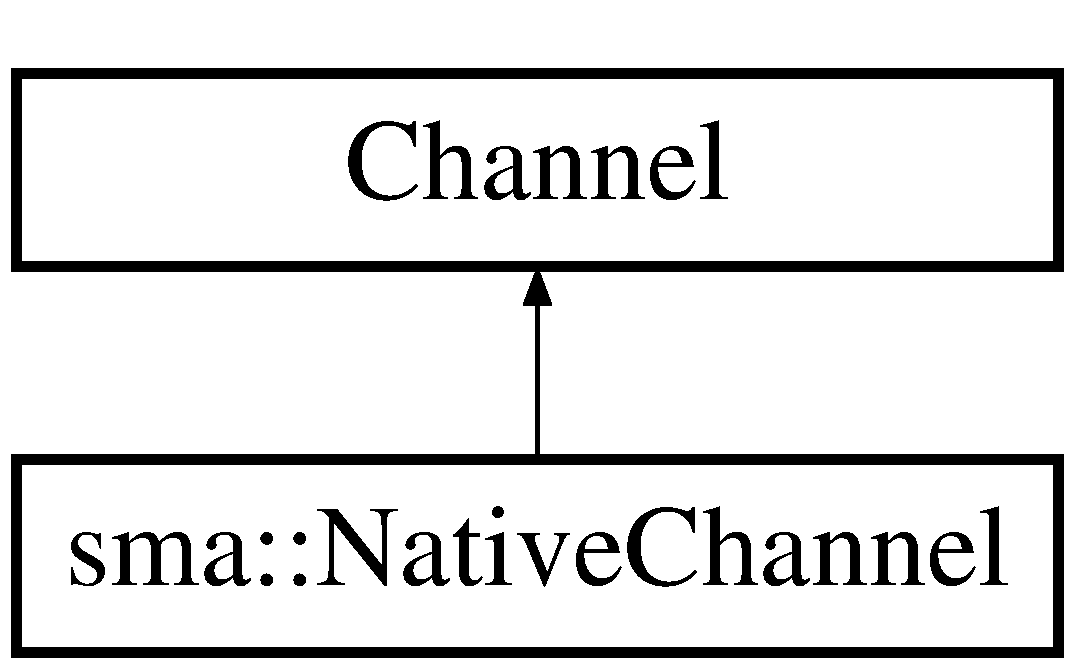
\includegraphics[height=2.000000cm]{classsma_1_1NativeChannel}
\end{center}
\end{figure}
\subsection*{Public Member Functions}
\begin{DoxyCompactItemize}
\item 
\hypertarget{classsma_1_1NativeChannel_a881188f3abc8d7efe7d51d487241336f}{{\bfseries Native\-Channel} (Native\-Socket $\ast$socket)}\label{classsma_1_1NativeChannel_a881188f3abc8d7efe7d51d487241336f}

\item 
\hypertarget{classsma_1_1NativeChannel_ae9d90e3a5e2b7f8632da8e6412a9a9d8}{{\bfseries Native\-Channel} (std\-::vector$<$ Native\-Socket $\ast$ $>$ sockets)}\label{classsma_1_1NativeChannel_ae9d90e3a5e2b7f8632da8e6412a9a9d8}

\item 
\hypertarget{classsma_1_1NativeChannel_a752a87f5c84b60cfeee7c2efad575c37}{std\-::size\-\_\-t {\bfseries wait\-\_\-for\-\_\-read} (std\-::uint8\-\_\-t $\ast$dst, std\-::size\-\_\-t len) override}\label{classsma_1_1NativeChannel_a752a87f5c84b60cfeee7c2efad575c37}

\item 
\hypertarget{classsma_1_1NativeChannel_a61802878daf5645c92eb3b149b1c9d53}{void {\bfseries select} ()}\label{classsma_1_1NativeChannel_a61802878daf5645c92eb3b149b1c9d53}

\end{DoxyCompactItemize}


The documentation for this class was generated from the following file\-:\begin{DoxyCompactItemize}
\item 
android/core/include/sma/android/select\-\_\-channel.\-hpp\end{DoxyCompactItemize}

\hypertarget{structsma_1_1Neighbor}{\section{sma\-:\-:Neighbor Struct Reference}
\label{structsma_1_1Neighbor}\index{sma\-::\-Neighbor@{sma\-::\-Neighbor}}
}
\subsection*{Public Types}
\begin{DoxyCompactItemize}
\item 
\hypertarget{structsma_1_1Neighbor_a0ccc8da7cad8ef5bfb7e4f3f0e7ec49f}{using {\bfseries clock} = \hyperlink{structsma_1_1chrono_1_1system__clock}{sma\-::chrono\-::system\-\_\-clock}}\label{structsma_1_1Neighbor_a0ccc8da7cad8ef5bfb7e4f3f0e7ec49f}

\item 
\hypertarget{structsma_1_1Neighbor_a98d826a60714532d4fb24b70dd698520}{using {\bfseries time\-\_\-point} = clock\-::time\-\_\-point}\label{structsma_1_1Neighbor_a98d826a60714532d4fb24b70dd698520}

\end{DoxyCompactItemize}
\subsection*{Public Member Functions}
\begin{DoxyCompactItemize}
\item 
\hypertarget{structsma_1_1Neighbor_af35fd2a83e83e026b813f1dfd7eac92e}{bool {\bfseries is\-\_\-new} () const }\label{structsma_1_1Neighbor_af35fd2a83e83e026b813f1dfd7eac92e}

\item 
\hypertarget{structsma_1_1Neighbor_a72f897f9f70a92c877859f58d2c4f86c}{{\footnotesize template$<$typename D $>$ }\\bool {\bfseries older\-\_\-than} (D age) const }\label{structsma_1_1Neighbor_a72f897f9f70a92c877859f58d2c4f86c}

\item 
\hypertarget{structsma_1_1Neighbor_a239b8183ca0a2b9e1c78cdae730c1ced}{void {\bfseries touch} ()}\label{structsma_1_1Neighbor_a239b8183ca0a2b9e1c78cdae730c1ced}

\end{DoxyCompactItemize}
\subsection*{Public Attributes}
\begin{DoxyCompactItemize}
\item 
\hypertarget{structsma_1_1Neighbor_a480c12dade1086301c11e30a2fd07f45}{time\-\_\-point {\bfseries first\-\_\-seen}}\label{structsma_1_1Neighbor_a480c12dade1086301c11e30a2fd07f45}

\item 
\hypertarget{structsma_1_1Neighbor_a0fe58aa478b0b11e5d20cba65b04fc9d}{time\-\_\-point {\bfseries last\-\_\-seen}}\label{structsma_1_1Neighbor_a0fe58aa478b0b11e5d20cba65b04fc9d}

\end{DoxyCompactItemize}


The documentation for this struct was generated from the following file\-:\begin{DoxyCompactItemize}
\item 
include/sma/neighbor.\-hpp\end{DoxyCompactItemize}

\hypertarget{classsma_1_1NeighborHelper}{\section{sma\-:\-:Neighbor\-Helper Class Reference}
\label{classsma_1_1NeighborHelper}\index{sma\-::\-Neighbor\-Helper@{sma\-::\-Neighbor\-Helper}}
}
Inheritance diagram for sma\-:\-:Neighbor\-Helper\-:\begin{figure}[H]
\begin{center}
\leavevmode
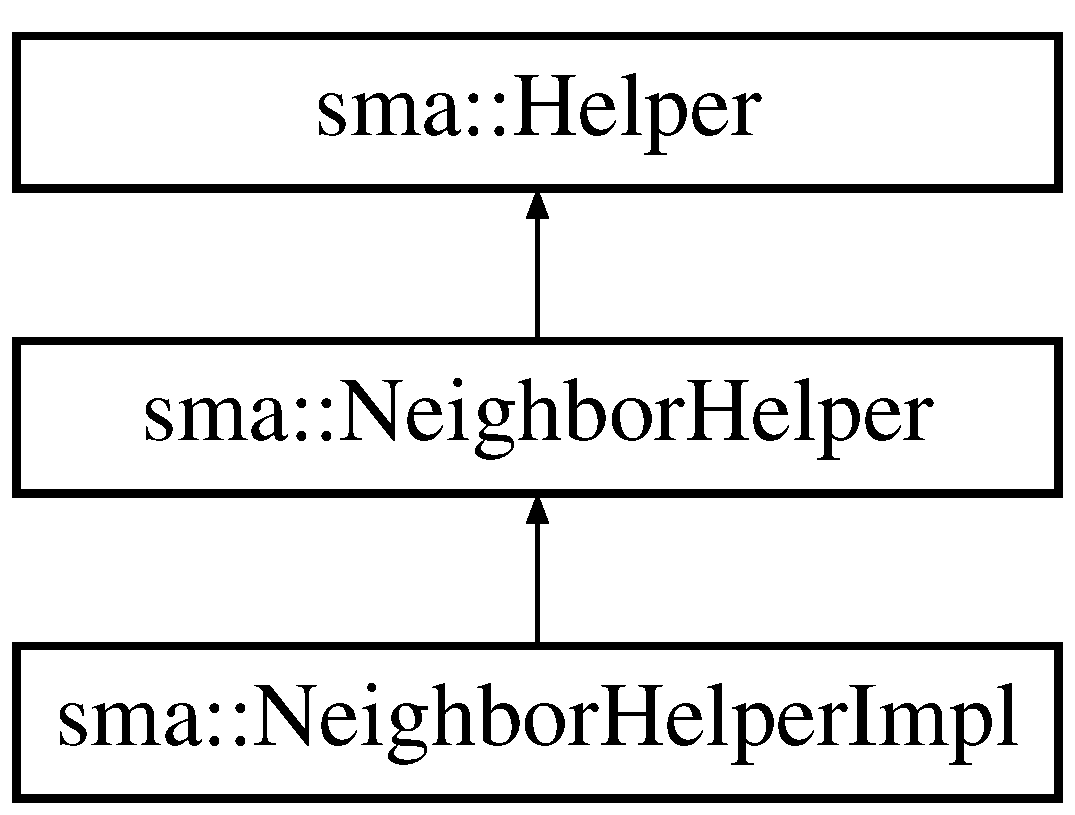
\includegraphics[height=3.000000cm]{classsma_1_1NeighborHelper}
\end{center}
\end{figure}
\subsection*{Public Member Functions}
\begin{DoxyCompactItemize}
\item 
\hypertarget{classsma_1_1NeighborHelper_af7ff94940765d61ad2633e6dd67a2503}{{\bfseries Neighbor\-Helper} (\hyperlink{classsma_1_1CcnNode}{Ccn\-Node} \&node)}\label{classsma_1_1NeighborHelper_af7ff94940765d61ad2633e6dd67a2503}

\item 
\hypertarget{classsma_1_1NeighborHelper_a289846f1dc67c7e8c2a4147416e54749}{virtual void {\bfseries receive} (\hyperlink{structsma_1_1MessageHeader}{Message\-Header} header, \hyperlink{structsma_1_1Beacon}{Beacon} msg)=0}\label{classsma_1_1NeighborHelper_a289846f1dc67c7e8c2a4147416e54749}

\end{DoxyCompactItemize}
\subsection*{Additional Inherited Members}


The documentation for this class was generated from the following files\-:\begin{DoxyCompactItemize}
\item 
include/sma/neighborhelper.\-hpp\item 
src/neighborhelper.\-cpp\end{DoxyCompactItemize}

\hypertarget{classsma_1_1NeighborHelperImpl}{\section{sma\-:\-:Neighbor\-Helper\-Impl Class Reference}
\label{classsma_1_1NeighborHelperImpl}\index{sma\-::\-Neighbor\-Helper\-Impl@{sma\-::\-Neighbor\-Helper\-Impl}}
}
Inheritance diagram for sma\-:\-:Neighbor\-Helper\-Impl\-:\begin{figure}[H]
\begin{center}
\leavevmode
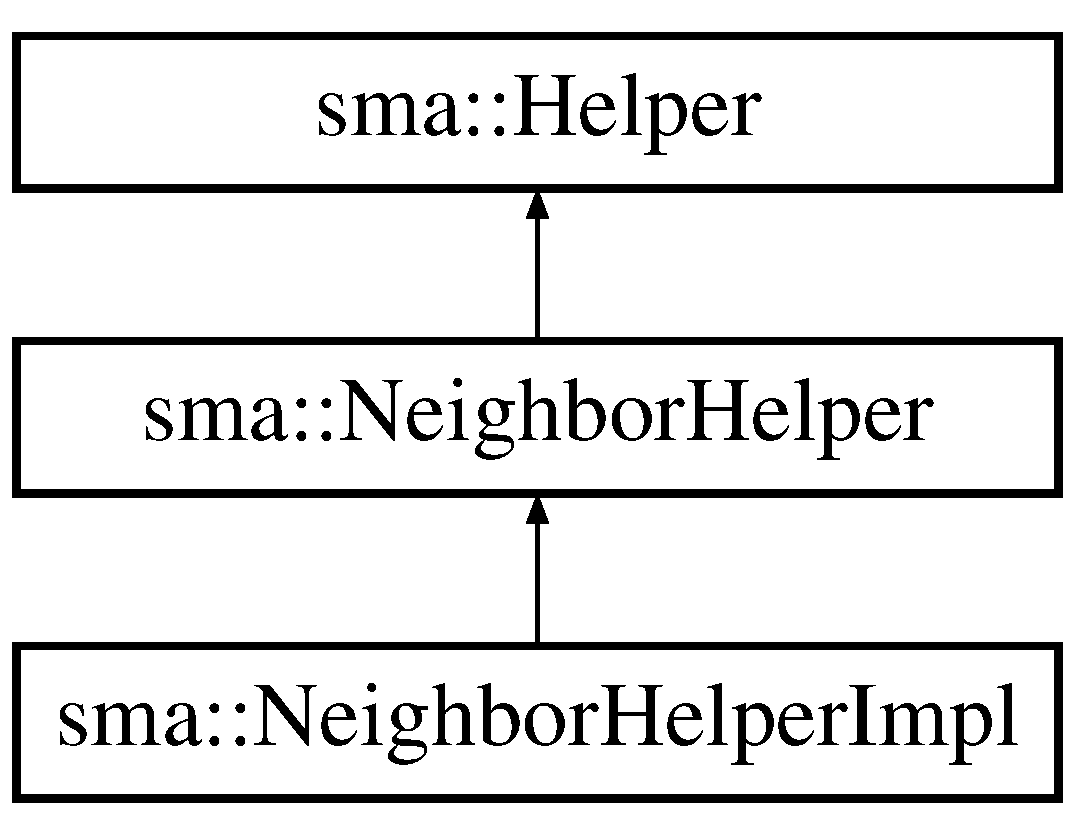
\includegraphics[height=3.000000cm]{classsma_1_1NeighborHelperImpl}
\end{center}
\end{figure}
\subsection*{Public Member Functions}
\begin{DoxyCompactItemize}
\item 
\hypertarget{classsma_1_1NeighborHelperImpl_a77420dbc9ea439a082a85b31461a2b10}{{\bfseries Neighbor\-Helper\-Impl} (\hyperlink{classsma_1_1CcnNode}{Ccn\-Node} \&node)}\label{classsma_1_1NeighborHelperImpl_a77420dbc9ea439a082a85b31461a2b10}

\item 
\hypertarget{classsma_1_1NeighborHelperImpl_a016eb3acd4c3194ddb9a2ca9432a207c}{void {\bfseries receive} (\hyperlink{structsma_1_1MessageHeader}{Message\-Header} header, \hyperlink{structsma_1_1Beacon}{Beacon} msg) override}\label{classsma_1_1NeighborHelperImpl_a016eb3acd4c3194ddb9a2ca9432a207c}

\end{DoxyCompactItemize}
\subsection*{Additional Inherited Members}


The documentation for this class was generated from the following files\-:\begin{DoxyCompactItemize}
\item 
include/sma/neighborhelperimpl.\-hpp\item 
src/neighborhelperimpl.\-cpp\end{DoxyCompactItemize}

\hypertarget{classsma_1_1NeighborTable}{\section{sma\-:\-:Neighbor\-Table Class Reference}
\label{classsma_1_1NeighborTable}\index{sma\-::\-Neighbor\-Table@{sma\-::\-Neighbor\-Table}}
}
\subsection*{Public Types}
\begin{DoxyCompactItemize}
\item 
\hypertarget{classsma_1_1NeighborTable_ace1f1d7df173e5c91265bc954b624c4f}{using {\bfseries value\-\_\-type} = table\-\_\-type\-::value\-\_\-type}\label{classsma_1_1NeighborTable_ace1f1d7df173e5c91265bc954b624c4f}

\item 
\hypertarget{classsma_1_1NeighborTable_aff8b8fb7623aeb232c7a7b567fe5e51e}{using {\bfseries iterator} = table\-\_\-type\-::iterator}\label{classsma_1_1NeighborTable_aff8b8fb7623aeb232c7a7b567fe5e51e}

\item 
\hypertarget{classsma_1_1NeighborTable_ac596e231fc7a1202882853d4b8c1f93a}{using {\bfseries const\-\_\-iterator} = table\-\_\-type\-::const\-\_\-iterator}\label{classsma_1_1NeighborTable_ac596e231fc7a1202882853d4b8c1f93a}

\item 
\hypertarget{classsma_1_1NeighborTable_ace2540e6f895d104730ac7c1e79178d8}{using {\bfseries size\-\_\-type} = table\-\_\-type\-::size\-\_\-type}\label{classsma_1_1NeighborTable_ace2540e6f895d104730ac7c1e79178d8}

\end{DoxyCompactItemize}
\subsection*{Public Member Functions}
\begin{DoxyCompactItemize}
\item 
\hypertarget{classsma_1_1NeighborTable_aab743ad677e50024ea361c2d71f03e9d}{\hyperlink{structsma_1_1Neighbor}{Neighbor} {\bfseries update} (\hyperlink{structsma_1_1NodeId}{Node\-Id} node)}\label{classsma_1_1NeighborTable_aab743ad677e50024ea361c2d71f03e9d}

\item 
\hypertarget{classsma_1_1NeighborTable_a9b7d314dece28e3036162ba55af82c6b}{void {\bfseries prune} (std\-::chrono\-::milliseconds max\-\_\-age, std\-::vector$<$ value\-\_\-type $>$ $\ast$optional\-\_\-pruned\-\_\-out=nullptr)}\label{classsma_1_1NeighborTable_a9b7d314dece28e3036162ba55af82c6b}

\item 
\hypertarget{classsma_1_1NeighborTable_ab81c16e2a0ab5a20021a463a5e2f23ee}{size\-\_\-type {\bfseries size} () const }\label{classsma_1_1NeighborTable_ab81c16e2a0ab5a20021a463a5e2f23ee}

\item 
\hypertarget{classsma_1_1NeighborTable_af15c63b21b2dbd50605f397010d2aa51}{bool {\bfseries empty} () const }\label{classsma_1_1NeighborTable_af15c63b21b2dbd50605f397010d2aa51}

\item 
\hypertarget{classsma_1_1NeighborTable_a75ccee9fcdc5672ddd62a203cb997b83}{iterator {\bfseries begin} ()}\label{classsma_1_1NeighborTable_a75ccee9fcdc5672ddd62a203cb997b83}

\item 
\hypertarget{classsma_1_1NeighborTable_aa3ee1e004c5000adde847f26652cb7f5}{iterator {\bfseries end} ()}\label{classsma_1_1NeighborTable_aa3ee1e004c5000adde847f26652cb7f5}

\item 
\hypertarget{classsma_1_1NeighborTable_ae65f184f456941cf5b1124a59d32ae87}{const\-\_\-iterator {\bfseries cbegin} () const }\label{classsma_1_1NeighborTable_ae65f184f456941cf5b1124a59d32ae87}

\item 
\hypertarget{classsma_1_1NeighborTable_a8d9588e4d14bd5c8dcf1f9c3ca0c83da}{const\-\_\-iterator {\bfseries cend} () const }\label{classsma_1_1NeighborTable_a8d9588e4d14bd5c8dcf1f9c3ca0c83da}

\end{DoxyCompactItemize}


The documentation for this class was generated from the following files\-:\begin{DoxyCompactItemize}
\item 
include/sma/neighbortable.\-hpp\item 
src/neighbortable.\-cpp\end{DoxyCompactItemize}

\hypertarget{classel_1_1base_1_1NoCopy}{\section{el\-:\-:base\-:\-:No\-Copy Class Reference}
\label{classel_1_1base_1_1NoCopy}\index{el\-::base\-::\-No\-Copy@{el\-::base\-::\-No\-Copy}}
}


Internal helper class that prevent copy constructor for class.  




{\ttfamily \#include $<$logimpl.\-hpp$>$}

Inheritance diagram for el\-:\-:base\-:\-:No\-Copy\-:\begin{figure}[H]
\begin{center}
\leavevmode
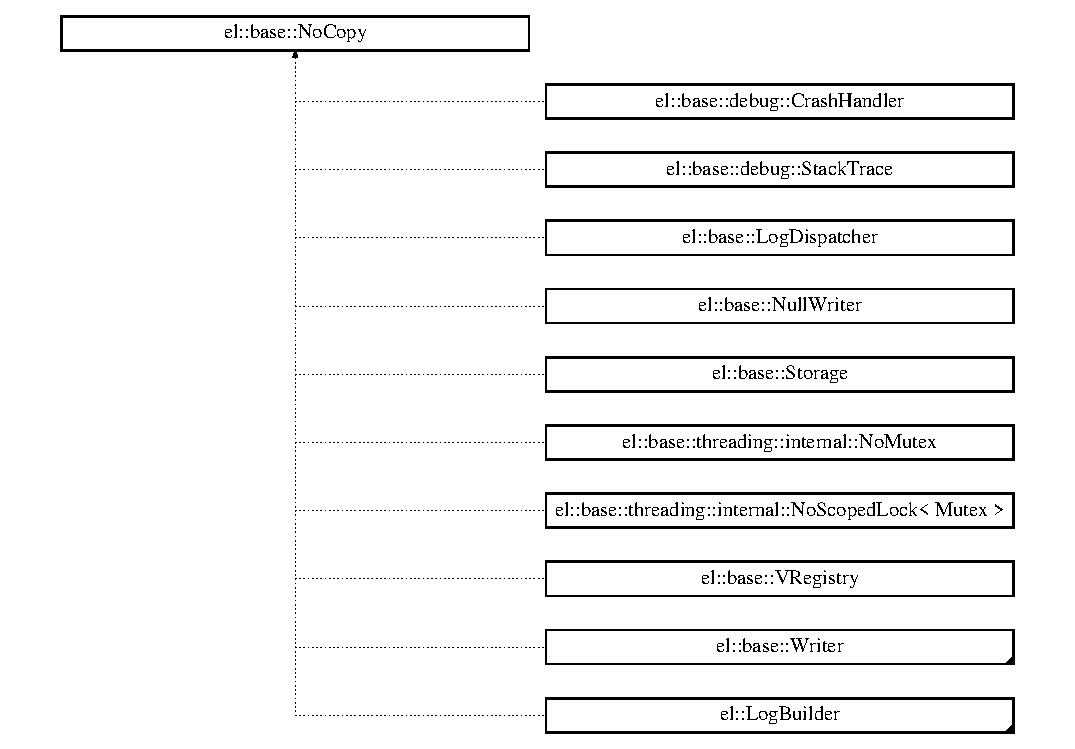
\includegraphics[height=9.625000cm]{classel_1_1base_1_1NoCopy}
\end{center}
\end{figure}


\subsection{Detailed Description}
Internal helper class that prevent copy constructor for class. 

When using this class simply inherit it privately 

The documentation for this class was generated from the following file\-:\begin{DoxyCompactItemize}
\item 
include/sma/io/detail/logimpl.\-hpp\end{DoxyCompactItemize}

\hypertarget{structsma_1_1NodeId}{\section{sma\-:\-:Node\-Id Struct Reference}
\label{structsma_1_1NodeId}\index{sma\-::\-Node\-Id@{sma\-::\-Node\-Id}}
}
\subsection*{Public Types}
\begin{DoxyCompactItemize}
\item 
\hypertarget{structsma_1_1NodeId_a9f433208c6dc97683dd46bdc119d3d16}{using {\bfseries value\-\_\-type} = std\-::uint16\-\_\-t}\label{structsma_1_1NodeId_a9f433208c6dc97683dd46bdc119d3d16}

\end{DoxyCompactItemize}
\subsection*{Public Member Functions}
\begin{DoxyCompactItemize}
\item 
\hypertarget{structsma_1_1NodeId_ad7fbb134091a71ac0da11da29e7eebfd}{{\footnotesize template$<$typename T , typename std\-::enable\-\_\-if$<$ std\-::is\-\_\-integral$<$ T $>$\-::value \&\&sizeof(\-T) $>$  = sizeof(value\-\_\-type)$>$ }\\\-::type $\ast$\hyperlink{structsma_1_1NodeId}{Node\-Id} \& {\bfseries operator=} (\hyperlink{structsma_1_1NodeId}{Node\-Id} const \&)=default}\label{structsma_1_1NodeId_ad7fbb134091a71ac0da11da29e7eebfd}

\item 
\hypertarget{structsma_1_1NodeId_a56db372577d1f02ad2c5cd4663cc3092}{bool {\bfseries operator==} (\hyperlink{structsma_1_1NodeId}{Node\-Id} const \&r) const }\label{structsma_1_1NodeId_a56db372577d1f02ad2c5cd4663cc3092}

\item 
\hypertarget{structsma_1_1NodeId_afbb14b857e41a6869b42dd8d68ebd949}{bool {\bfseries operator!=} (\hyperlink{structsma_1_1NodeId}{Node\-Id} const \&r) const }\label{structsma_1_1NodeId_afbb14b857e41a6869b42dd8d68ebd949}

\item 
\hypertarget{structsma_1_1NodeId_ab549f1f3c03d09d5c1f7a4a10ceac4dd}{{\bfseries operator std\-::uint64\-\_\-t} () const }\label{structsma_1_1NodeId_ab549f1f3c03d09d5c1f7a4a10ceac4dd}

\item 
\hypertarget{structsma_1_1NodeId_abd9a737860d66dc98e1c02589b3a399b}{{\bfseries operator std\-::uint32\-\_\-t} () const }\label{structsma_1_1NodeId_abd9a737860d66dc98e1c02589b3a399b}

\item 
\hypertarget{structsma_1_1NodeId_ab0f29c870c2d8db7f32815e49902b956}{{\bfseries operator std\-::uint16\-\_\-t} () const }\label{structsma_1_1NodeId_ab0f29c870c2d8db7f32815e49902b956}

\item 
\hypertarget{structsma_1_1NodeId_a5df5ee9e720a02c2be0a45ea283914ee}{{\bfseries operator std\-::string} () const }\label{structsma_1_1NodeId_a5df5ee9e720a02c2be0a45ea283914ee}

\end{DoxyCompactItemize}
\subsection*{Friends}
\begin{DoxyCompactItemize}
\item 
\hypertarget{structsma_1_1NodeId_a7b8015dab4fec84b715849906d4deebf}{struct {\bfseries std\-::hash$<$ Node\-Id $>$}}\label{structsma_1_1NodeId_a7b8015dab4fec84b715849906d4deebf}

\end{DoxyCompactItemize}


The documentation for this struct was generated from the following file\-:\begin{DoxyCompactItemize}
\item 
include/sma/nodeid.\-hpp\end{DoxyCompactItemize}

\hypertarget{classel_1_1base_1_1threading_1_1internal_1_1NoMutex}{\section{el\-:\-:base\-:\-:threading\-:\-:internal\-:\-:No\-Mutex Class Reference}
\label{classel_1_1base_1_1threading_1_1internal_1_1NoMutex}\index{el\-::base\-::threading\-::internal\-::\-No\-Mutex@{el\-::base\-::threading\-::internal\-::\-No\-Mutex}}
}


Mutex wrapper used when multi-\/threading is disabled.  




{\ttfamily \#include $<$logimpl.\-hpp$>$}

Inheritance diagram for el\-:\-:base\-:\-:threading\-:\-:internal\-:\-:No\-Mutex\-:\begin{figure}[H]
\begin{center}
\leavevmode
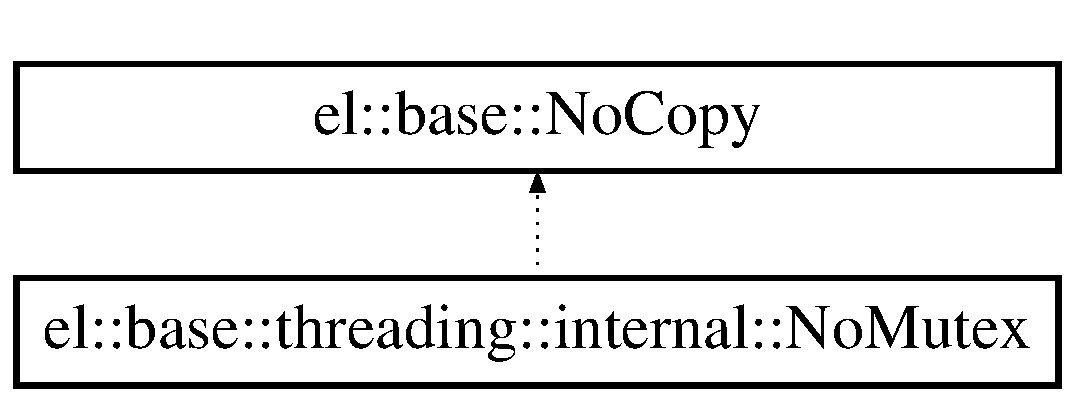
\includegraphics[height=2.000000cm]{classel_1_1base_1_1threading_1_1internal_1_1NoMutex}
\end{center}
\end{figure}
\subsection*{Public Member Functions}
\begin{DoxyCompactItemize}
\item 
\hypertarget{classel_1_1base_1_1threading_1_1internal_1_1NoMutex_a3b38e4e9411c924daa70d358cf561b3c}{void {\bfseries lock} (void)}\label{classel_1_1base_1_1threading_1_1internal_1_1NoMutex_a3b38e4e9411c924daa70d358cf561b3c}

\item 
\hypertarget{classel_1_1base_1_1threading_1_1internal_1_1NoMutex_a4c0c35a99cf41f26a7608fed5609d6ae}{bool {\bfseries try\-\_\-lock} (void)}\label{classel_1_1base_1_1threading_1_1internal_1_1NoMutex_a4c0c35a99cf41f26a7608fed5609d6ae}

\item 
\hypertarget{classel_1_1base_1_1threading_1_1internal_1_1NoMutex_a5a248c97fee2ef0087526f2f8d3cd26e}{void {\bfseries unlock} (void)}\label{classel_1_1base_1_1threading_1_1internal_1_1NoMutex_a5a248c97fee2ef0087526f2f8d3cd26e}

\end{DoxyCompactItemize}


\subsection{Detailed Description}
Mutex wrapper used when multi-\/threading is disabled. 

The documentation for this class was generated from the following file\-:\begin{DoxyCompactItemize}
\item 
include/sma/io/detail/logimpl.\-hpp\end{DoxyCompactItemize}

\hypertarget{classel_1_1base_1_1threading_1_1internal_1_1NoScopedLock}{\section{el\-:\-:base\-:\-:threading\-:\-:internal\-:\-:No\-Scoped\-Lock$<$ Mutex $>$ Class Template Reference}
\label{classel_1_1base_1_1threading_1_1internal_1_1NoScopedLock}\index{el\-::base\-::threading\-::internal\-::\-No\-Scoped\-Lock$<$ Mutex $>$@{el\-::base\-::threading\-::internal\-::\-No\-Scoped\-Lock$<$ Mutex $>$}}
}


Lock guard wrapper used when multi-\/threading is disabled.  




{\ttfamily \#include $<$logimpl.\-hpp$>$}

Inheritance diagram for el\-:\-:base\-:\-:threading\-:\-:internal\-:\-:No\-Scoped\-Lock$<$ Mutex $>$\-:\begin{figure}[H]
\begin{center}
\leavevmode
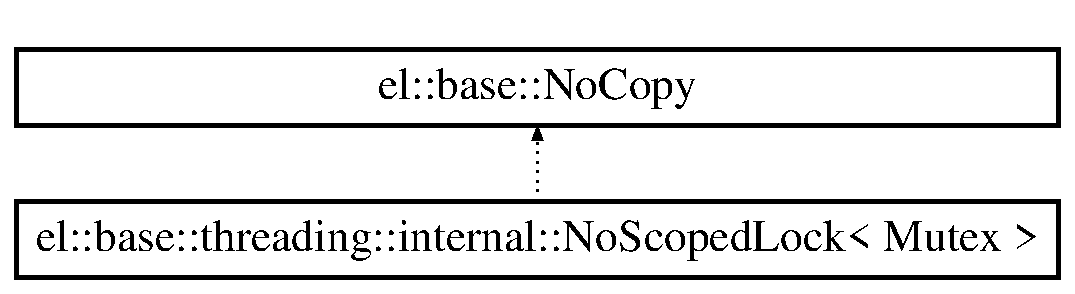
\includegraphics[height=2.000000cm]{classel_1_1base_1_1threading_1_1internal_1_1NoScopedLock}
\end{center}
\end{figure}
\subsection*{Public Member Functions}
\begin{DoxyCompactItemize}
\item 
\hypertarget{classel_1_1base_1_1threading_1_1internal_1_1NoScopedLock_a020f8cea6e83f40ea29662ef57a58235}{{\bfseries No\-Scoped\-Lock} (\hyperlink{classel_1_1base_1_1threading_1_1internal_1_1NoMutex}{Mutex} \&)}\label{classel_1_1base_1_1threading_1_1internal_1_1NoScopedLock_a020f8cea6e83f40ea29662ef57a58235}

\end{DoxyCompactItemize}


\subsection{Detailed Description}
\subsubsection*{template$<$typename Mutex$>$class el\-::base\-::threading\-::internal\-::\-No\-Scoped\-Lock$<$ Mutex $>$}

Lock guard wrapper used when multi-\/threading is disabled. 

The documentation for this class was generated from the following file\-:\begin{DoxyCompactItemize}
\item 
include/sma/io/detail/logimpl.\-hpp\end{DoxyCompactItemize}

\hypertarget{structsma_1_1Ns3AsyncProxy}{\section{sma\-:\-:Ns3\-Async\-Proxy Struct Reference}
\label{structsma_1_1Ns3AsyncProxy}\index{sma\-::\-Ns3\-Async\-Proxy@{sma\-::\-Ns3\-Async\-Proxy}}
}
\subsection*{Public Member Functions}
\begin{DoxyCompactItemize}
\item 
\hypertarget{structsma_1_1Ns3AsyncProxy_aec89508638f43643f00e3e6af2e00e6a}{void {\bfseries operator()} ()}\label{structsma_1_1Ns3AsyncProxy_aec89508638f43643f00e3e6af2e00e6a}

\end{DoxyCompactItemize}
\subsection*{Public Attributes}
\begin{DoxyCompactItemize}
\item 
\hypertarget{structsma_1_1Ns3AsyncProxy_af24e504290490b05704bb6cb15fa914d}{ns3\-::\-Event\-Id {\bfseries id}}\label{structsma_1_1Ns3AsyncProxy_af24e504290490b05704bb6cb15fa914d}

\item 
\hypertarget{structsma_1_1Ns3AsyncProxy_ae35a52fb06e848a8e45c32d819408d11}{std\-::function$<$ void()$>$ {\bfseries target}}\label{structsma_1_1Ns3AsyncProxy_ae35a52fb06e848a8e45c32d819408d11}

\end{DoxyCompactItemize}


The documentation for this struct was generated from the following file\-:\begin{DoxyCompactItemize}
\item 
ns3/src/async.\-cpp\end{DoxyCompactItemize}

\hypertarget{classsma_1_1Ns3InetLink}{\section{sma\-:\-:Ns3\-Inet\-Link Class Reference}
\label{classsma_1_1Ns3InetLink}\index{sma\-::\-Ns3\-Inet\-Link@{sma\-::\-Ns3\-Inet\-Link}}
}
Inheritance diagram for sma\-:\-:Ns3\-Inet\-Link\-:\begin{figure}[H]
\begin{center}
\leavevmode
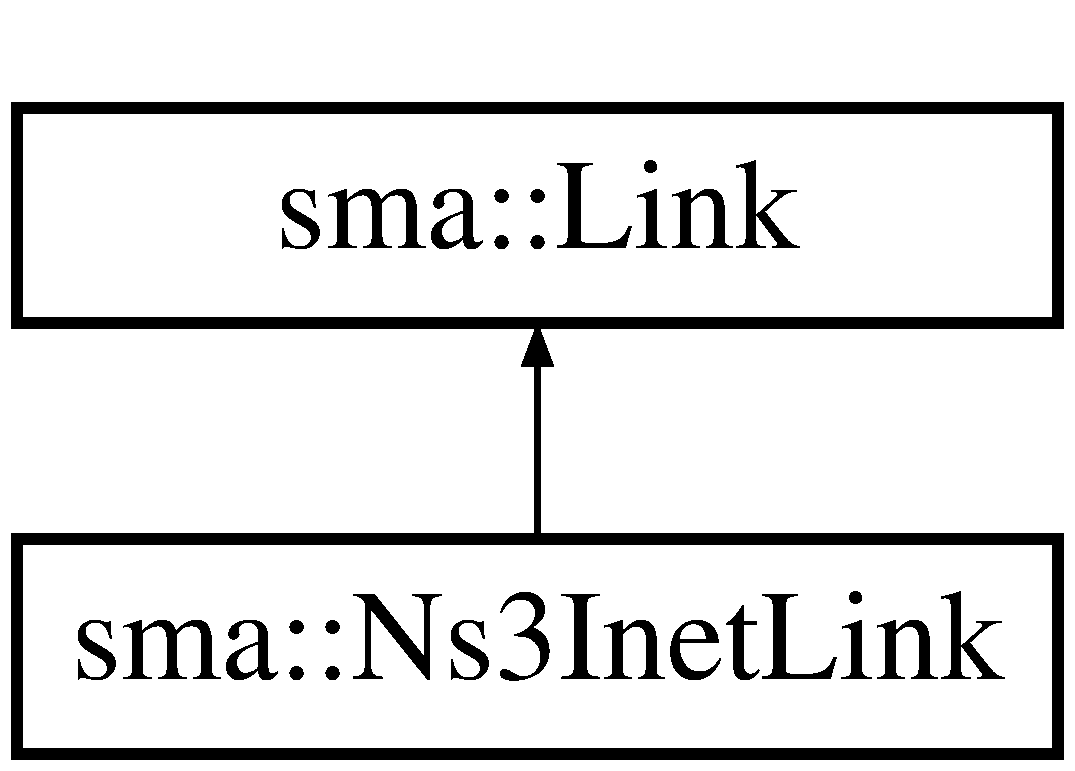
\includegraphics[height=2.000000cm]{classsma_1_1Ns3InetLink}
\end{center}
\end{figure}
\subsection*{Public Member Functions}
\begin{DoxyCompactItemize}
\item 
\hypertarget{classsma_1_1Ns3InetLink_af2c974c49f521b18f241f6757ff8c0df}{{\bfseries Ns3\-Inet\-Link} (ns3\-::\-Ptr$<$ ns3\-::\-Node $>$ this\-\_\-node)}\label{classsma_1_1Ns3InetLink_af2c974c49f521b18f241f6757ff8c0df}

\item 
\hypertarget{classsma_1_1Ns3InetLink_aa7c5f097857d2bcdb8e7ca0618922413}{{\bfseries Ns3\-Inet\-Link} (\hyperlink{classsma_1_1Ns3InetLink}{Ns3\-Inet\-Link} const \&)=delete}\label{classsma_1_1Ns3InetLink_aa7c5f097857d2bcdb8e7ca0618922413}

\item 
\hypertarget{classsma_1_1Ns3InetLink_a6853c05d4cf43277fd252d737de4db47}{\hyperlink{classsma_1_1Ns3InetLink}{Ns3\-Inet\-Link} \& {\bfseries operator=} (\hyperlink{classsma_1_1Ns3InetLink}{Ns3\-Inet\-Link} const \&)=delete}\label{classsma_1_1Ns3InetLink_a6853c05d4cf43277fd252d737de4db47}

\item 
\hypertarget{classsma_1_1Ns3InetLink_aa715856ee5898ad647f3ba459854a7dc}{std\-::size\-\_\-t {\bfseries read} (void $\ast$dst, std\-::size\-\_\-t size) override}\label{classsma_1_1Ns3InetLink_aa715856ee5898ad647f3ba459854a7dc}

\item 
\hypertarget{classsma_1_1Ns3InetLink_a1ccd46880c20145a96639f76c1172ec7}{std\-::size\-\_\-t {\bfseries write} (void const $\ast$src, std\-::size\-\_\-t size) override}\label{classsma_1_1Ns3InetLink_a1ccd46880c20145a96639f76c1172ec7}

\item 
\hypertarget{classsma_1_1Ns3InetLink_ace9d75ecd205a9ebf166c30538b600f3}{void {\bfseries close} () override}\label{classsma_1_1Ns3InetLink_ace9d75ecd205a9ebf166c30538b600f3}

\end{DoxyCompactItemize}
\subsection*{Additional Inherited Members}


The documentation for this class was generated from the following files\-:\begin{DoxyCompactItemize}
\item 
ns3/include/sma/ns3/ns3inetlink.\-hpp\item 
ns3/src/ns3inetlink.\-cpp\end{DoxyCompactItemize}

\hypertarget{classsma_1_1Ns3NodeContainer}{\section{sma\-:\-:Ns3\-Node\-Container Class Reference}
\label{classsma_1_1Ns3NodeContainer}\index{sma\-::\-Ns3\-Node\-Container@{sma\-::\-Ns3\-Node\-Container}}
}
Inheritance diagram for sma\-:\-:Ns3\-Node\-Container\-:\begin{figure}[H]
\begin{center}
\leavevmode
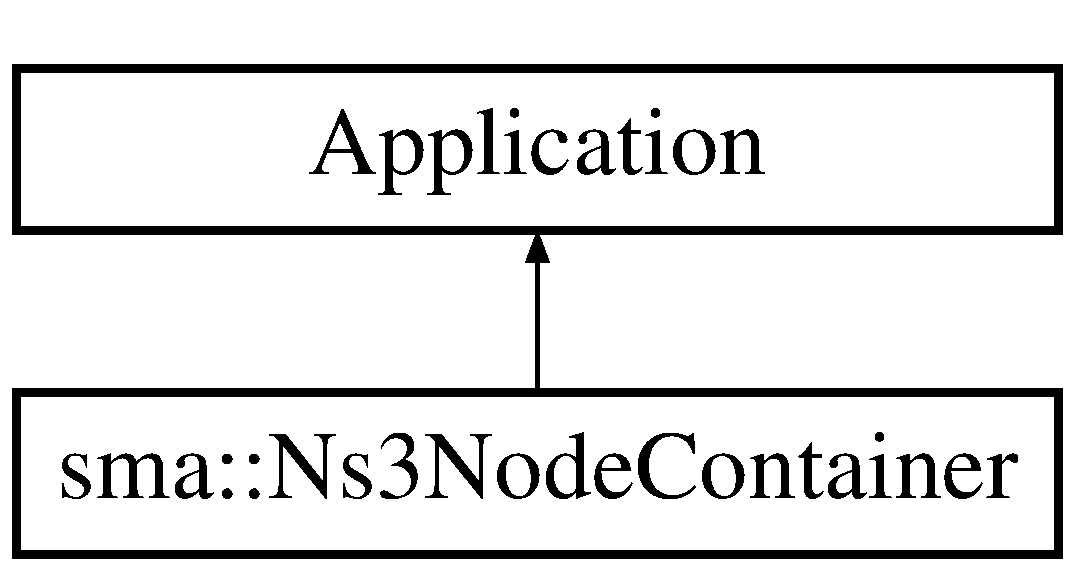
\includegraphics[height=2.000000cm]{classsma_1_1Ns3NodeContainer}
\end{center}
\end{figure}
\subsection*{Public Member Functions}
\begin{DoxyCompactItemize}
\item 
\hypertarget{classsma_1_1Ns3NodeContainer_a7d448aa3a6289e5d1f73beb8982f60e3}{{\bfseries Ns3\-Node\-Container} (\hyperlink{classsma_1_1Ns3NodeContainer}{Ns3\-Node\-Container} const \&)=delete}\label{classsma_1_1Ns3NodeContainer_a7d448aa3a6289e5d1f73beb8982f60e3}

\item 
\hypertarget{classsma_1_1Ns3NodeContainer_a959f4a15ef1b756bf9cb82ecc54d9cf2}{\hyperlink{classsma_1_1Ns3NodeContainer}{Ns3\-Node\-Container} \& {\bfseries operator=} (\hyperlink{classsma_1_1Ns3NodeContainer}{Ns3\-Node\-Container} const \&)=delete}\label{classsma_1_1Ns3NodeContainer_a959f4a15ef1b756bf9cb82ecc54d9cf2}

\item 
\hypertarget{classsma_1_1Ns3NodeContainer_a62b15de00156c17973fbcb8bdbf55509}{void {\bfseries add\-\_\-component} (std\-::unique\-\_\-ptr$<$ \hyperlink{classsma_1_1Component}{Component} $>$ c)}\label{classsma_1_1Ns3NodeContainer_a62b15de00156c17973fbcb8bdbf55509}

\item 
\hypertarget{classsma_1_1Ns3NodeContainer_a34e264662e39424402ef9011d108aca2}{{\footnotesize template$<$typename A , typename Duration , typename... Args$>$ }\\void \hyperlink{classsma_1_1Ns3NodeContainer_a34e264662e39424402ef9011d108aca2}{act\-\_\-emplace\-\_\-back} (Duration const \&delay, Args \&\&...args)}\label{classsma_1_1Ns3NodeContainer_a34e264662e39424402ef9011d108aca2}

\begin{DoxyCompactList}\small\item\em Construct an action of type A with the given arguments and sort it into the existing actions in reverse-\/chronological order (most to least distant in the future). If this action occurs farther in the future than all others then this is O(1). \end{DoxyCompactList}\item 
\hypertarget{classsma_1_1Ns3NodeContainer_a90dea220baa998cdb45030fe4617cfec}{{\footnotesize template$<$typename A , typename Duration , typename... Args$>$ }\\void \hyperlink{classsma_1_1Ns3NodeContainer_a90dea220baa998cdb45030fe4617cfec}{act\-\_\-emplace\-\_\-front} (Duration const \&delay, Args \&\&...args)}\label{classsma_1_1Ns3NodeContainer_a90dea220baa998cdb45030fe4617cfec}

\begin{DoxyCompactList}\small\item\em Construct an action of type A with the given arguments and sort it into the existing actions in chronological order. If this action occurs sooner than all others then this is O(1). \end{DoxyCompactList}\item 
\hypertarget{classsma_1_1Ns3NodeContainer_adc0a677c70d532797182a36ebfceb13f}{void \hyperlink{classsma_1_1Ns3NodeContainer_adc0a677c70d532797182a36ebfceb13f}{act\-\_\-schedule} (\hyperlink{structsma_1_1Action}{Action} \&act)}\label{classsma_1_1Ns3NodeContainer_adc0a677c70d532797182a36ebfceb13f}

\begin{DoxyCompactList}\small\item\em Schedule the next action to run at the given time. \end{DoxyCompactList}\item 
\hypertarget{classsma_1_1Ns3NodeContainer_af2e85bc06c3ce1e4704b83e75238eb2c}{void \hyperlink{classsma_1_1Ns3NodeContainer_af2e85bc06c3ce1e4704b83e75238eb2c}{act\-\_\-next} ()}\label{classsma_1_1Ns3NodeContainer_af2e85bc06c3ce1e4704b83e75238eb2c}

\begin{DoxyCompactList}\small\item\em Dequeue the next action, run it (potentially enqueing additional actions), and schedule the next soonest (potentially new) action. \end{DoxyCompactList}\end{DoxyCompactItemize}
\subsection*{Static Public Member Functions}
\begin{DoxyCompactItemize}
\item 
\hypertarget{classsma_1_1Ns3NodeContainer_a5b5b1fecf2f2ef358b6f10fc39f21455}{static ns3\-::\-Type\-Id {\bfseries Type\-Id} ()}\label{classsma_1_1Ns3NodeContainer_a5b5b1fecf2f2ef358b6f10fc39f21455}

\end{DoxyCompactItemize}
\subsection*{Public Attributes}
\begin{DoxyCompactItemize}
\item 
\hypertarget{classsma_1_1Ns3NodeContainer_a20aa2dad2564577082af144530eec729}{std\-::unique\-\_\-ptr$<$ \hyperlink{classsma_1_1CcnNode}{Ccn\-Node} $>$ {\bfseries node}}\label{classsma_1_1Ns3NodeContainer_a20aa2dad2564577082af144530eec729}

\end{DoxyCompactItemize}
\subsection*{Protected Member Functions}
\begin{DoxyCompactItemize}
\item 
\hypertarget{classsma_1_1Ns3NodeContainer_a493122868e16dac6a995199ee283e51c}{virtual void {\bfseries Do\-Dispose} () override}\label{classsma_1_1Ns3NodeContainer_a493122868e16dac6a995199ee283e51c}

\item 
\hypertarget{classsma_1_1Ns3NodeContainer_a0a9999e48d25caee6421a95896be6486}{virtual void {\bfseries Start\-Application} () override}\label{classsma_1_1Ns3NodeContainer_a0a9999e48d25caee6421a95896be6486}

\item 
\hypertarget{classsma_1_1Ns3NodeContainer_a6ebdc650d95f836932f76db067e5dbf2}{virtual void {\bfseries Stop\-Application} () override}\label{classsma_1_1Ns3NodeContainer_a6ebdc650d95f836932f76db067e5dbf2}

\end{DoxyCompactItemize}


The documentation for this class was generated from the following files\-:\begin{DoxyCompactItemize}
\item 
ns3/include/sma/ns3/ns3nodecontainer.\-hpp\item 
ns3/src/ns3nodecontainer.\-cpp\end{DoxyCompactItemize}

\hypertarget{classel_1_1base_1_1NullWriter}{\section{el\-:\-:base\-:\-:Null\-Writer Class Reference}
\label{classel_1_1base_1_1NullWriter}\index{el\-::base\-::\-Null\-Writer@{el\-::base\-::\-Null\-Writer}}
}


Writes nothing -\/ Used when certain log is disabled.  




{\ttfamily \#include $<$logimpl.\-hpp$>$}

Inheritance diagram for el\-:\-:base\-:\-:Null\-Writer\-:\begin{figure}[H]
\begin{center}
\leavevmode
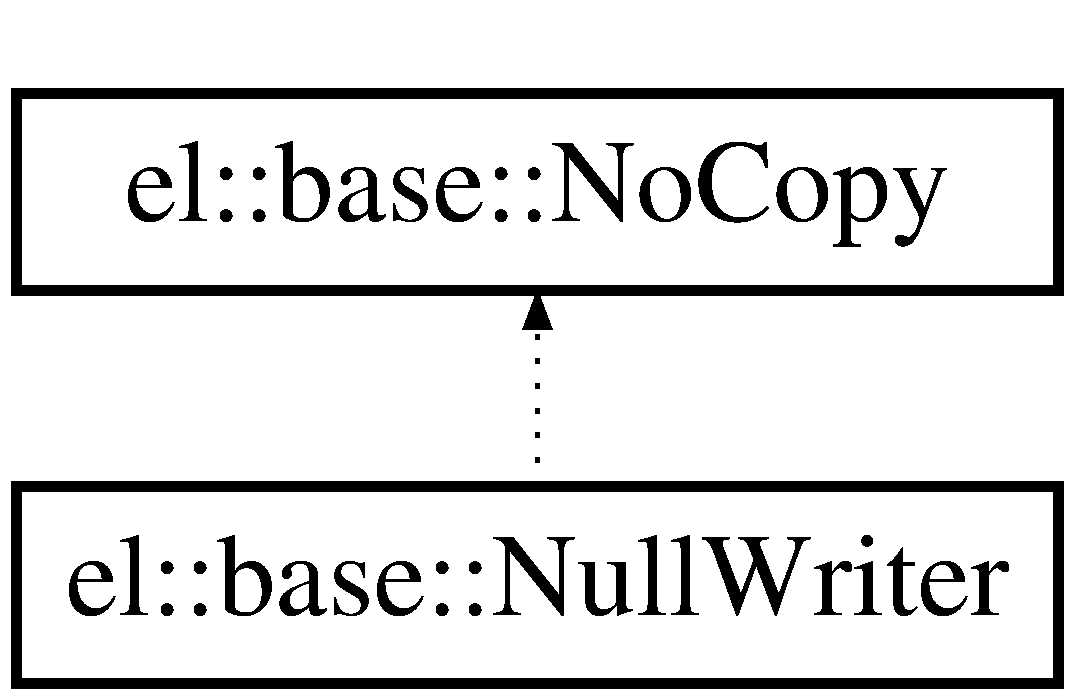
\includegraphics[height=2.000000cm]{classel_1_1base_1_1NullWriter}
\end{center}
\end{figure}
\subsection*{Public Member Functions}
\begin{DoxyCompactItemize}
\item 
\hypertarget{classel_1_1base_1_1NullWriter_a39cb7d47986d70c2b4e9d78d1482da7d}{\hyperlink{classel_1_1base_1_1NullWriter}{Null\-Writer} \& {\bfseries operator$<$$<$} (std\-::ostream \&($\ast$)(std\-::ostream \&))}\label{classel_1_1base_1_1NullWriter_a39cb7d47986d70c2b4e9d78d1482da7d}

\item 
\hypertarget{classel_1_1base_1_1NullWriter_a57cb0f5d93ebac076b8ef94d6eff65a2}{{\footnotesize template$<$typename T $>$ }\\\hyperlink{classel_1_1base_1_1NullWriter}{Null\-Writer} \& {\bfseries operator$<$$<$} (const T \&)}\label{classel_1_1base_1_1NullWriter_a57cb0f5d93ebac076b8ef94d6eff65a2}

\end{DoxyCompactItemize}


\subsection{Detailed Description}
Writes nothing -\/ Used when certain log is disabled. 

The documentation for this class was generated from the following file\-:\begin{DoxyCompactItemize}
\item 
include/sma/io/detail/logimpl.\-hpp\end{DoxyCompactItemize}

\hypertarget{classel_1_1base_1_1utils_1_1OS}{\section{el\-:\-:base\-:\-:utils\-:\-:O\-S Class Reference}
\label{classel_1_1base_1_1utils_1_1OS}\index{el\-::base\-::utils\-::\-O\-S@{el\-::base\-::utils\-::\-O\-S}}
}


Operating System helper static class used internally. You should not use it.  




{\ttfamily \#include $<$logimpl.\-hpp$>$}

Inheritance diagram for el\-:\-:base\-:\-:utils\-:\-:O\-S\-:\begin{figure}[H]
\begin{center}
\leavevmode
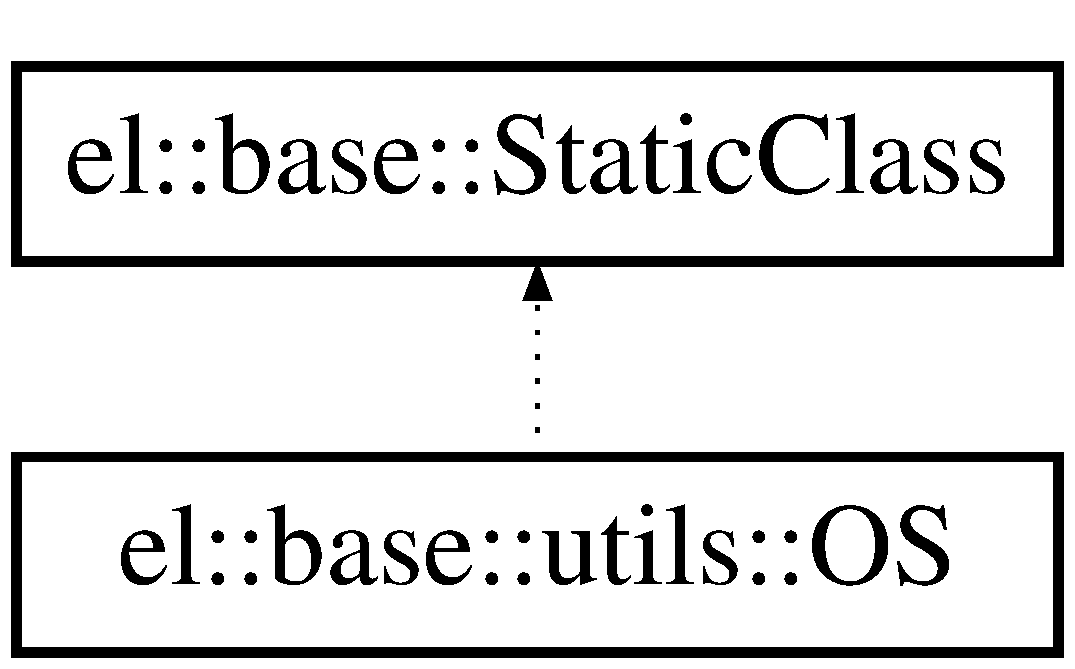
\includegraphics[height=2.000000cm]{classel_1_1base_1_1utils_1_1OS}
\end{center}
\end{figure}
\subsection*{Static Public Member Functions}
\begin{DoxyCompactItemize}
\item 
static const std\-::string \hyperlink{classel_1_1base_1_1utils_1_1OS_a91304c76c872459eaa9fdb3466367cd3}{get\-Bash\-Output} (const char $\ast$command)
\begin{DoxyCompactList}\small\item\em Runs command on terminal and returns the output. \end{DoxyCompactList}\item 
static std\-::string \hyperlink{classel_1_1base_1_1utils_1_1OS_a91540f3d8c87bd121e55fc39270eac3c}{get\-Environment\-Variable} (const char $\ast$variable\-Name, const char $\ast$default\-Val, const char $\ast$alternative\-Bash\-Command=nullptr)
\begin{DoxyCompactList}\small\item\em Gets environment variable. This is cross-\/platform and C\-R\-T safe (for V\-C++) \end{DoxyCompactList}\item 
\hypertarget{classel_1_1base_1_1utils_1_1OS_ac7839ecd50e379dbdfcfce130906386e}{static std\-::string \hyperlink{classel_1_1base_1_1utils_1_1OS_ac7839ecd50e379dbdfcfce130906386e}{current\-User} (void)}\label{classel_1_1base_1_1utils_1_1OS_ac7839ecd50e379dbdfcfce130906386e}

\begin{DoxyCompactList}\small\item\em Gets current username. \end{DoxyCompactList}\item 
static std\-::string \hyperlink{classel_1_1base_1_1utils_1_1OS_aae4fdf83828228fc440f8a875c5942b0}{current\-Host} (void)
\begin{DoxyCompactList}\small\item\em Gets current host name or computer name. \end{DoxyCompactList}\item 
\hypertarget{classel_1_1base_1_1utils_1_1OS_a2c941329a14ce0ea920f57779857864c}{static bool \hyperlink{classel_1_1base_1_1utils_1_1OS_a2c941329a14ce0ea920f57779857864c}{term\-Supports\-Color} (void)}\label{classel_1_1base_1_1utils_1_1OS_a2c941329a14ce0ea920f57779857864c}

\begin{DoxyCompactList}\small\item\em Whether or not terminal supports colors. \end{DoxyCompactList}\end{DoxyCompactItemize}


\subsection{Detailed Description}
Operating System helper static class used internally. You should not use it. 

\subsection{Member Function Documentation}
\hypertarget{classel_1_1base_1_1utils_1_1OS_aae4fdf83828228fc440f8a875c5942b0}{\index{el\-::base\-::utils\-::\-O\-S@{el\-::base\-::utils\-::\-O\-S}!current\-Host@{current\-Host}}
\index{current\-Host@{current\-Host}!el::base::utils::OS@{el\-::base\-::utils\-::\-O\-S}}
\subsubsection[{current\-Host}]{\setlength{\rightskip}{0pt plus 5cm}static std\-::string el\-::base\-::utils\-::\-O\-S\-::current\-Host (
\begin{DoxyParamCaption}
\item[{void}]{}
\end{DoxyParamCaption}
)\hspace{0.3cm}{\ttfamily [inline]}, {\ttfamily [static]}}}\label{classel_1_1base_1_1utils_1_1OS_aae4fdf83828228fc440f8a875c5942b0}


Gets current host name or computer name. 

For android systems this is device name with its manufacturer and model seperated by hyphen \hypertarget{classel_1_1base_1_1utils_1_1OS_a91304c76c872459eaa9fdb3466367cd3}{\index{el\-::base\-::utils\-::\-O\-S@{el\-::base\-::utils\-::\-O\-S}!get\-Bash\-Output@{get\-Bash\-Output}}
\index{get\-Bash\-Output@{get\-Bash\-Output}!el::base::utils::OS@{el\-::base\-::utils\-::\-O\-S}}
\subsubsection[{get\-Bash\-Output}]{\setlength{\rightskip}{0pt plus 5cm}static const std\-::string el\-::base\-::utils\-::\-O\-S\-::get\-Bash\-Output (
\begin{DoxyParamCaption}
\item[{const char $\ast$}]{command}
\end{DoxyParamCaption}
)\hspace{0.3cm}{\ttfamily [inline]}, {\ttfamily [static]}}}\label{classel_1_1base_1_1utils_1_1OS_a91304c76c872459eaa9fdb3466367cd3}


Runs command on terminal and returns the output. 

This is applicable only on unix based systems, for all other \hyperlink{classel_1_1base_1_1utils_1_1OS}{O\-S}, an empty string is returned. 
\begin{DoxyParams}{Parameters}
{\em command} & Bash command \\
\hline
\end{DoxyParams}
\begin{DoxyReturn}{Returns}
Result of bash output or empty string if no result found. 
\end{DoxyReturn}
\hypertarget{classel_1_1base_1_1utils_1_1OS_a91540f3d8c87bd121e55fc39270eac3c}{\index{el\-::base\-::utils\-::\-O\-S@{el\-::base\-::utils\-::\-O\-S}!get\-Environment\-Variable@{get\-Environment\-Variable}}
\index{get\-Environment\-Variable@{get\-Environment\-Variable}!el::base::utils::OS@{el\-::base\-::utils\-::\-O\-S}}
\subsubsection[{get\-Environment\-Variable}]{\setlength{\rightskip}{0pt plus 5cm}static std\-::string el\-::base\-::utils\-::\-O\-S\-::get\-Environment\-Variable (
\begin{DoxyParamCaption}
\item[{const char $\ast$}]{variable\-Name, }
\item[{const char $\ast$}]{default\-Val, }
\item[{const char $\ast$}]{alternative\-Bash\-Command = {\ttfamily nullptr}}
\end{DoxyParamCaption}
)\hspace{0.3cm}{\ttfamily [inline]}, {\ttfamily [static]}}}\label{classel_1_1base_1_1utils_1_1OS_a91540f3d8c87bd121e55fc39270eac3c}


Gets environment variable. This is cross-\/platform and C\-R\-T safe (for V\-C++) 


\begin{DoxyParams}{Parameters}
{\em variable\-Name} & Environment variable name \\
\hline
{\em default\-Val} & If no environment variable or value found the value to return by default \\
\hline
{\em alternative\-Bash\-Command} & If environment variable not found what would be alternative bash command in order to look for value user is looking for. E.\-g, for 'user' alternative command will 'whoami' \\
\hline
\end{DoxyParams}


The documentation for this class was generated from the following file\-:\begin{DoxyCompactItemize}
\item 
include/sma/io/detail/logimpl.\-hpp\end{DoxyCompactItemize}

\hypertarget{classel_1_1Configurations_1_1Parser}{\section{el\-:\-:Configurations\-:\-:Parser Class Reference}
\label{classel_1_1Configurations_1_1Parser}\index{el\-::\-Configurations\-::\-Parser@{el\-::\-Configurations\-::\-Parser}}
}


\hyperlink{classel_1_1Configurations_1_1Parser}{Parser} used internally to parse configurations from file or text.  




{\ttfamily \#include $<$logimpl.\-hpp$>$}

Inheritance diagram for el\-:\-:Configurations\-:\-:Parser\-:\begin{figure}[H]
\begin{center}
\leavevmode
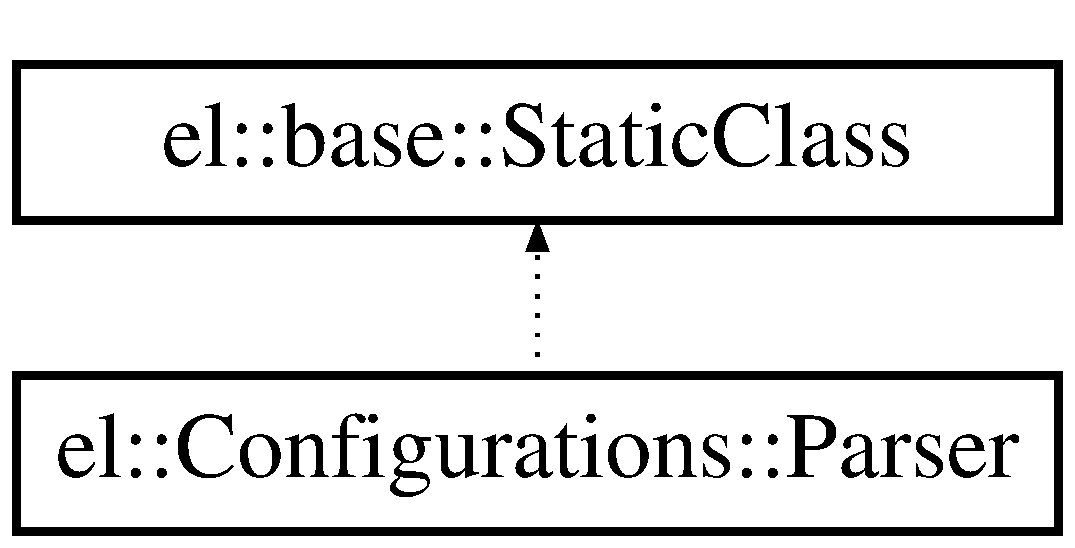
\includegraphics[height=2.000000cm]{classel_1_1Configurations_1_1Parser}
\end{center}
\end{figure}
\subsection*{Static Public Member Functions}
\begin{DoxyCompactItemize}
\item 
static bool \hyperlink{classel_1_1Configurations_1_1Parser_a45def5007bf368c4d2a505af58cd94c2}{parse\-From\-File} (const std\-::string \&\hyperlink{classel_1_1Configurations_a18df64bb5cd97bee672160290133141c}{configuration\-File}, \hyperlink{classel_1_1Configurations}{Configurations} $\ast$sender, \hyperlink{classel_1_1Configurations}{Configurations} $\ast$base=nullptr)
\begin{DoxyCompactList}\small\item\em Parses configuration from file. \end{DoxyCompactList}\item 
static bool \hyperlink{classel_1_1Configurations_1_1Parser_a39ec1b06f673e8155a83d66e08229129}{parse\-From\-Text} (const std\-::string \&configurations\-String, \hyperlink{classel_1_1Configurations}{Configurations} $\ast$sender, \hyperlink{classel_1_1Configurations}{Configurations} $\ast$base=nullptr)
\begin{DoxyCompactList}\small\item\em Parse configurations from configuration string. \end{DoxyCompactList}\end{DoxyCompactItemize}
\subsection*{Friends}
\begin{DoxyCompactItemize}
\item 
\hypertarget{classel_1_1Configurations_1_1Parser_a6efe246b312d02731fb0e1d120c0331d}{class {\bfseries el\-::\-Loggers}}\label{classel_1_1Configurations_1_1Parser_a6efe246b312d02731fb0e1d120c0331d}

\end{DoxyCompactItemize}


\subsection{Detailed Description}
\hyperlink{classel_1_1Configurations_1_1Parser}{Parser} used internally to parse configurations from file or text. 

This class makes use of \hyperlink{classel_1_1base_1_1utils_1_1Str}{base\-::utils\-::\-Str}. You should not need this unless you are working on some tool for Easylogging++ 

\subsection{Member Function Documentation}
\hypertarget{classel_1_1Configurations_1_1Parser_a45def5007bf368c4d2a505af58cd94c2}{\index{el\-::\-Configurations\-::\-Parser@{el\-::\-Configurations\-::\-Parser}!parse\-From\-File@{parse\-From\-File}}
\index{parse\-From\-File@{parse\-From\-File}!el::Configurations::Parser@{el\-::\-Configurations\-::\-Parser}}
\subsubsection[{parse\-From\-File}]{\setlength{\rightskip}{0pt plus 5cm}static bool el\-::\-Configurations\-::\-Parser\-::parse\-From\-File (
\begin{DoxyParamCaption}
\item[{const std\-::string \&}]{configuration\-File, }
\item[{{\bf Configurations} $\ast$}]{sender, }
\item[{{\bf Configurations} $\ast$}]{base = {\ttfamily nullptr}}
\end{DoxyParamCaption}
)\hspace{0.3cm}{\ttfamily [inline]}, {\ttfamily [static]}}}\label{classel_1_1Configurations_1_1Parser_a45def5007bf368c4d2a505af58cd94c2}


Parses configuration from file. 


\begin{DoxyParams}{Parameters}
{\em configuration\-File} & Full path to configuration file \\
\hline
{\em sender} & Sender configurations pointer. Usually 'this' is used from calling class \\
\hline
{\em base} & \hyperlink{classel_1_1Configurations}{Configurations} to base new configuration repository off. This value is used when you want to use existing \hyperlink{classel_1_1Configurations}{Configurations} to base all the values and then set rest of configuration via configuration file. \\
\hline
\end{DoxyParams}
\begin{DoxyReturn}{Returns}
True if successfully parsed, false otherwise. You may define '\-\_\-\-S\-T\-O\-P\-\_\-\-O\-N\-\_\-\-F\-I\-R\-S\-T\-\_\-\-E\-L\-P\-P\-\_\-\-A\-S\-S\-E\-R\-T\-I\-O\-N' to make sure you do not proceed without successful parse. 
\end{DoxyReturn}
\hypertarget{classel_1_1Configurations_1_1Parser_a39ec1b06f673e8155a83d66e08229129}{\index{el\-::\-Configurations\-::\-Parser@{el\-::\-Configurations\-::\-Parser}!parse\-From\-Text@{parse\-From\-Text}}
\index{parse\-From\-Text@{parse\-From\-Text}!el::Configurations::Parser@{el\-::\-Configurations\-::\-Parser}}
\subsubsection[{parse\-From\-Text}]{\setlength{\rightskip}{0pt plus 5cm}static bool el\-::\-Configurations\-::\-Parser\-::parse\-From\-Text (
\begin{DoxyParamCaption}
\item[{const std\-::string \&}]{configurations\-String, }
\item[{{\bf Configurations} $\ast$}]{sender, }
\item[{{\bf Configurations} $\ast$}]{base = {\ttfamily nullptr}}
\end{DoxyParamCaption}
)\hspace{0.3cm}{\ttfamily [inline]}, {\ttfamily [static]}}}\label{classel_1_1Configurations_1_1Parser_a39ec1b06f673e8155a83d66e08229129}


Parse configurations from configuration string. 

This configuration string has same syntax as configuration file contents. Make sure all the necessary new line characters are provided. You may define '\-\_\-\-S\-T\-O\-P\-\_\-\-O\-N\-\_\-\-F\-I\-R\-S\-T\-\_\-\-E\-L\-P\-P\-\_\-\-A\-S\-S\-E\-R\-T\-I\-O\-N' to make sure you do not proceed without successful parse (This is recommended) 
\begin{DoxyParams}{Parameters}
{\em configurations\-String} & \\
\hline
{\em sender} & Sender configurations pointer. Usually 'this' is used from calling class \\
\hline
{\em base} & \hyperlink{classel_1_1Configurations}{Configurations} to base new configuration repository off. This value is used when you want to use existing \hyperlink{classel_1_1Configurations}{Configurations} to base all the values and then set rest of configuration via configuration text. \\
\hline
\end{DoxyParams}
\begin{DoxyReturn}{Returns}
True if successfully parsed, false otherwise. 
\end{DoxyReturn}


The documentation for this class was generated from the following file\-:\begin{DoxyCompactItemize}
\item 
include/sma/io/detail/logimpl.\-hpp\end{DoxyCompactItemize}

\hypertarget{classel_1_1base_1_1PerformanceTracker}{\section{el\-:\-:base\-:\-:Performance\-Tracker Class Reference}
\label{classel_1_1base_1_1PerformanceTracker}\index{el\-::base\-::\-Performance\-Tracker@{el\-::base\-::\-Performance\-Tracker}}
}


Represents performance\-Tracker block of code that conditionally adds performance status to log either when goes outside the scope of when \hyperlink{classel_1_1base_1_1PerformanceTracker_aec9a6e149674c5782cc855e49aeb0aaf}{checkpoint()} is called.  




{\ttfamily \#include $<$logimpl.\-hpp$>$}

Inheritance diagram for el\-:\-:base\-:\-:Performance\-Tracker\-:\begin{figure}[H]
\begin{center}
\leavevmode
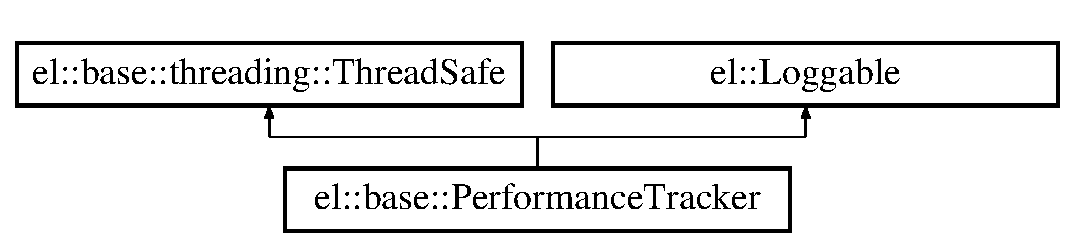
\includegraphics[height=2.000000cm]{classel_1_1base_1_1PerformanceTracker}
\end{center}
\end{figure}
\subsection*{Public Member Functions}
\begin{DoxyCompactItemize}
\item 
\hypertarget{classel_1_1base_1_1PerformanceTracker_a1794044d78f649890b2a0c48f56b11ef}{{\bfseries Performance\-Tracker} (const std\-::string \&block\-Name, \hyperlink{namespaceel_1_1base_a1b886858c6409097395b24b1bdf03c39}{base\-::\-Timestamp\-Unit} timestamp\-Unit=base\-::\-Timestamp\-Unit\-::\-Millisecond, const std\-::string \&logger\-Id=std\-::string(\-\_\-\-C\-U\-R\-R\-E\-N\-T\-\_\-\-F\-I\-L\-E\-\_\-\-P\-E\-R\-F\-O\-R\-M\-A\-N\-C\-E\-\_\-\-L\-O\-G\-G\-E\-R\-\_\-\-I\-D), bool scoped\-Log=true, \hyperlink{namespaceel_ab0ac6091262344c52dd2d3ad099e8e36}{Level} level=base\-::consts\-::k\-Performance\-Tracker\-Default\-Level)}\label{classel_1_1base_1_1PerformanceTracker_a1794044d78f649890b2a0c48f56b11ef}

\item 
\hypertarget{classel_1_1base_1_1PerformanceTracker_a49e655c1f414f904b2d6a9abb0d344f4}{\hyperlink{classel_1_1base_1_1PerformanceTracker_a49e655c1f414f904b2d6a9abb0d344f4}{Performance\-Tracker} (const \hyperlink{classel_1_1base_1_1PerformanceTracker}{Performance\-Tracker} \&t)}\label{classel_1_1base_1_1PerformanceTracker_a49e655c1f414f904b2d6a9abb0d344f4}

\begin{DoxyCompactList}\small\item\em Copy constructor. \end{DoxyCompactList}\item 
\hypertarget{classel_1_1base_1_1PerformanceTracker_aec9a6e149674c5782cc855e49aeb0aaf}{void \hyperlink{classel_1_1base_1_1PerformanceTracker_aec9a6e149674c5782cc855e49aeb0aaf}{checkpoint} (const std\-::string \&id=std\-::string(), const char $\ast$file=\-\_\-\-\_\-\-F\-I\-L\-E\-\_\-\-\_\-, unsigned long int line=\-\_\-\-\_\-\-L\-I\-N\-E\-\_\-\-\_\-, const char $\ast$func=\char`\"{}\char`\"{})}\label{classel_1_1base_1_1PerformanceTracker_aec9a6e149674c5782cc855e49aeb0aaf}

\begin{DoxyCompactList}\small\item\em A checkpoint for current performance\-Tracker block. \end{DoxyCompactList}\item 
\hypertarget{classel_1_1base_1_1PerformanceTracker_a3e0ebd666cc7416dc9b818418266161b}{\hyperlink{namespaceel_ab0ac6091262344c52dd2d3ad099e8e36}{Level} {\bfseries level} (void) const }\label{classel_1_1base_1_1PerformanceTracker_a3e0ebd666cc7416dc9b818418266161b}

\end{DoxyCompactItemize}
\subsection*{Friends}
\begin{DoxyCompactItemize}
\item 
\hypertarget{classel_1_1base_1_1PerformanceTracker_a7a4da7334b79856c37538484584207a6}{class {\bfseries el\-::\-Performance\-Tracking\-Data}}\label{classel_1_1base_1_1PerformanceTracker_a7a4da7334b79856c37538484584207a6}

\item 
\hypertarget{classel_1_1base_1_1PerformanceTracker_ad346c4097e3db22a7434e7da5aa9c5e3}{class {\bfseries base\-::\-Default\-Performance\-Tracking\-Callback}}\label{classel_1_1base_1_1PerformanceTracker_ad346c4097e3db22a7434e7da5aa9c5e3}

\end{DoxyCompactItemize}


\subsection{Detailed Description}
Represents performance\-Tracker block of code that conditionally adds performance status to log either when goes outside the scope of when \hyperlink{classel_1_1base_1_1PerformanceTracker_aec9a6e149674c5782cc855e49aeb0aaf}{checkpoint()} is called. 

The documentation for this class was generated from the following file\-:\begin{DoxyCompactItemize}
\item 
include/sma/io/detail/logimpl.\-hpp\end{DoxyCompactItemize}

\hypertarget{classel_1_1PerformanceTrackingCallback}{\section{el\-:\-:Performance\-Tracking\-Callback Class Reference}
\label{classel_1_1PerformanceTrackingCallback}\index{el\-::\-Performance\-Tracking\-Callback@{el\-::\-Performance\-Tracking\-Callback}}
}
Inheritance diagram for el\-:\-:Performance\-Tracking\-Callback\-:\begin{figure}[H]
\begin{center}
\leavevmode
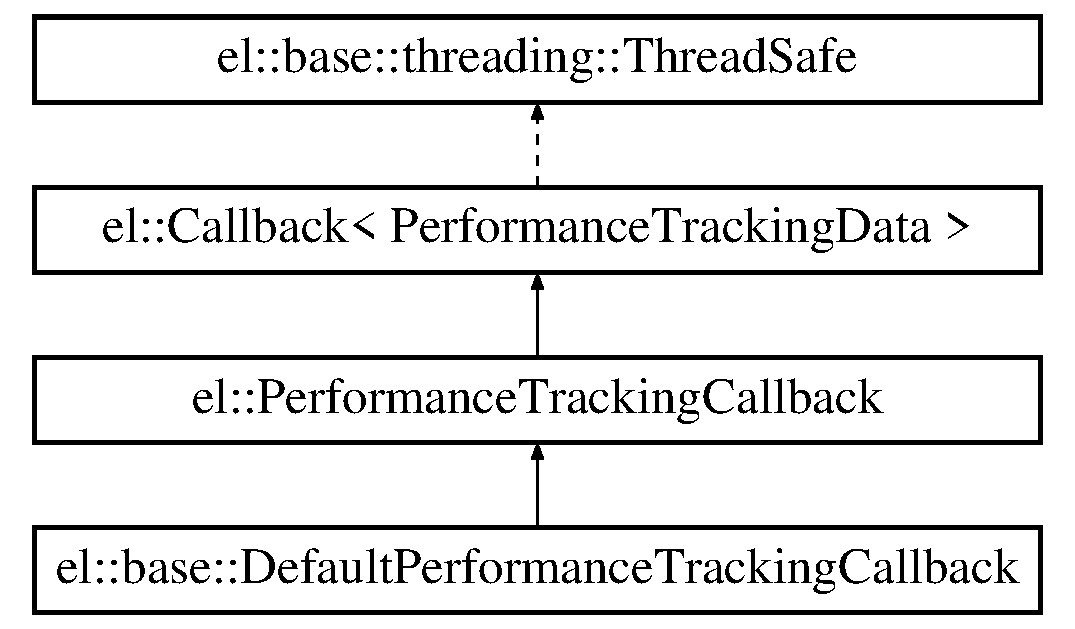
\includegraphics[height=4.000000cm]{classel_1_1PerformanceTrackingCallback}
\end{center}
\end{figure}
\subsection*{Friends}
\begin{DoxyCompactItemize}
\item 
\hypertarget{classel_1_1PerformanceTrackingCallback_a05f271f9cc2531409fe682c6ce0d9feb}{class {\bfseries base\-::\-Performance\-Tracker}}\label{classel_1_1PerformanceTrackingCallback_a05f271f9cc2531409fe682c6ce0d9feb}

\end{DoxyCompactItemize}
\subsection*{Additional Inherited Members}


The documentation for this class was generated from the following file\-:\begin{DoxyCompactItemize}
\item 
include/sma/io/detail/logimpl.\-hpp\end{DoxyCompactItemize}

\hypertarget{classel_1_1PerformanceTrackingData}{\section{el\-:\-:Performance\-Tracking\-Data Class Reference}
\label{classel_1_1PerformanceTrackingData}\index{el\-::\-Performance\-Tracking\-Data@{el\-::\-Performance\-Tracking\-Data}}
}
\subsection*{Public Types}
\begin{DoxyCompactItemize}
\item 
enum {\bfseries Data\-Type} \-: base\-::type\-::\-Enum\-Type \{ {\bfseries Checkpoint} = 1, 
{\bfseries Complete} = 2
 \}
\end{DoxyCompactItemize}
\subsection*{Public Member Functions}
\begin{DoxyCompactItemize}
\item 
\hypertarget{classel_1_1PerformanceTrackingData_afea4cb5328e6fdb27fcf8fc14acbdb40}{{\bfseries Performance\-Tracking\-Data} (Data\-Type data\-Type)}\label{classel_1_1PerformanceTrackingData_afea4cb5328e6fdb27fcf8fc14acbdb40}

\item 
\hypertarget{classel_1_1PerformanceTrackingData_a929601137dcef83759a563a94ef7aad4}{const std\-::string $\ast$ {\bfseries block\-Name} (void) const }\label{classel_1_1PerformanceTrackingData_a929601137dcef83759a563a94ef7aad4}

\item 
\hypertarget{classel_1_1PerformanceTrackingData_aeb2462e8a5c9e43a874a5bd441f22a17}{const struct timeval $\ast$ {\bfseries start\-Time} (void) const }\label{classel_1_1PerformanceTrackingData_aeb2462e8a5c9e43a874a5bd441f22a17}

\item 
\hypertarget{classel_1_1PerformanceTrackingData_a1828f5f7c3c1d879b73bb090df87dfb8}{const struct timeval $\ast$ {\bfseries end\-Time} (void) const }\label{classel_1_1PerformanceTrackingData_a1828f5f7c3c1d879b73bb090df87dfb8}

\item 
\hypertarget{classel_1_1PerformanceTrackingData_af6f072db1ae54343864bc19c2f99c186}{const struct timeval $\ast$ {\bfseries last\-Checkpoint\-Time} (void) const }\label{classel_1_1PerformanceTrackingData_af6f072db1ae54343864bc19c2f99c186}

\item 
\hypertarget{classel_1_1PerformanceTrackingData_ad19493aa3f826fdee28b59630ba3ecae}{const \hyperlink{classel_1_1base_1_1PerformanceTracker}{base\-::\-Performance\-Tracker} $\ast$ {\bfseries performance\-Tracker} (void) const }\label{classel_1_1PerformanceTrackingData_ad19493aa3f826fdee28b59630ba3ecae}

\item 
\hypertarget{classel_1_1PerformanceTrackingData_a38dc15a2015be16e23aafd3c36332dbf}{Performance\-Tracking\-Data\-::\-Data\-Type {\bfseries data\-Type} (void) const }\label{classel_1_1PerformanceTrackingData_a38dc15a2015be16e23aafd3c36332dbf}

\item 
\hypertarget{classel_1_1PerformanceTrackingData_a5bf01d3c580627a9a564cc6043275287}{bool {\bfseries first\-Checkpoint} (void) const }\label{classel_1_1PerformanceTrackingData_a5bf01d3c580627a9a564cc6043275287}

\item 
\hypertarget{classel_1_1PerformanceTrackingData_a17c92b7a9ea243eb37f3fa903ce6e06d}{std\-::string {\bfseries checkpoint\-Id} (void) const }\label{classel_1_1PerformanceTrackingData_a17c92b7a9ea243eb37f3fa903ce6e06d}

\item 
\hypertarget{classel_1_1PerformanceTrackingData_a51512448de4eb220514f193a2fc14849}{const char $\ast$ {\bfseries file} (void) const }\label{classel_1_1PerformanceTrackingData_a51512448de4eb220514f193a2fc14849}

\item 
\hypertarget{classel_1_1PerformanceTrackingData_a82529dd8d0c92bf377ec269cb4f69a45}{unsigned long int {\bfseries line} (void) const }\label{classel_1_1PerformanceTrackingData_a82529dd8d0c92bf377ec269cb4f69a45}

\item 
\hypertarget{classel_1_1PerformanceTrackingData_a12fe4fe91e83cbff7d5bb4736176ec30}{const char $\ast$ {\bfseries func} (void) const }\label{classel_1_1PerformanceTrackingData_a12fe4fe91e83cbff7d5bb4736176ec30}

\item 
\hypertarget{classel_1_1PerformanceTrackingData_a44a4c82d400155bd147eb455025c88fc}{const base\-::type\-::string\-\_\-t $\ast$ {\bfseries formatted\-Time\-Taken} () const }\label{classel_1_1PerformanceTrackingData_a44a4c82d400155bd147eb455025c88fc}

\item 
\hypertarget{classel_1_1PerformanceTrackingData_ae8ad846d155762ae7cab3fb67760f5a1}{const std\-::string \& {\bfseries logger\-Id} (void) const }\label{classel_1_1PerformanceTrackingData_ae8ad846d155762ae7cab3fb67760f5a1}

\end{DoxyCompactItemize}
\subsection*{Friends}
\begin{DoxyCompactItemize}
\item 
\hypertarget{classel_1_1PerformanceTrackingData_a6a4d7851e1984800be3c230f06a79528}{class {\bfseries el\-::base\-::\-Performance\-Tracker}}\label{classel_1_1PerformanceTrackingData_a6a4d7851e1984800be3c230f06a79528}

\end{DoxyCompactItemize}


The documentation for this class was generated from the following file\-:\begin{DoxyCompactItemize}
\item 
include/sma/io/detail/logimpl.\-hpp\end{DoxyCompactItemize}

\hypertarget{classel_1_1base_1_1PErrorWriter}{\section{el\-:\-:base\-:\-:P\-Error\-Writer Class Reference}
\label{classel_1_1base_1_1PErrorWriter}\index{el\-::base\-::\-P\-Error\-Writer@{el\-::base\-::\-P\-Error\-Writer}}
}
Inheritance diagram for el\-:\-:base\-:\-:P\-Error\-Writer\-:\begin{figure}[H]
\begin{center}
\leavevmode
\includegraphics[height=3.000000cm]{classel_1_1base_1_1PErrorWriter}
\end{center}
\end{figure}
\subsection*{Public Member Functions}
\begin{DoxyCompactItemize}
\item 
\hypertarget{classel_1_1base_1_1PErrorWriter_a60d1ff92d16e3927e2c4b5bb77d34092}{{\bfseries P\-Error\-Writer} (\hyperlink{namespaceel_ab0ac6091262344c52dd2d3ad099e8e36}{Level} level, const char $\ast$file, unsigned long int line, const char $\ast$func, \hyperlink{namespaceel_1_1base_a3aa2563d38e47388ba242a1694fc2839}{base\-::\-Dispatch\-Action} dispatch\-Action=base\-::\-Dispatch\-Action\-::\-Normal\-Log, base\-::type\-::\-Verbose\-Level verbose\-Level=0)}\label{classel_1_1base_1_1PErrorWriter_a60d1ff92d16e3927e2c4b5bb77d34092}

\end{DoxyCompactItemize}
\subsection*{Additional Inherited Members}


The documentation for this class was generated from the following file\-:\begin{DoxyCompactItemize}
\item 
include/sma/io/detail/logimpl.\-hpp\end{DoxyCompactItemize}

\hypertarget{classel_1_1base_1_1HitCounter_1_1Predicate}{\section{el\-:\-:base\-:\-:Hit\-Counter\-:\-:Predicate Class Reference}
\label{classel_1_1base_1_1HitCounter_1_1Predicate}\index{el\-::base\-::\-Hit\-Counter\-::\-Predicate@{el\-::base\-::\-Hit\-Counter\-::\-Predicate}}
}
\subsection*{Public Member Functions}
\begin{DoxyCompactItemize}
\item 
\hypertarget{classel_1_1base_1_1HitCounter_1_1Predicate_ab35f4f7da40df5a788c3984d097bb38c}{{\bfseries Predicate} (const char $\ast$filename, unsigned long int line\-Number)}\label{classel_1_1base_1_1HitCounter_1_1Predicate_ab35f4f7da40df5a788c3984d097bb38c}

\item 
\hypertarget{classel_1_1base_1_1HitCounter_1_1Predicate_ae07b1562a3c0ed38457401e60b80b0c5}{bool {\bfseries operator()} (const \hyperlink{classel_1_1base_1_1HitCounter}{Hit\-Counter} $\ast$counter)}\label{classel_1_1base_1_1HitCounter_1_1Predicate_ae07b1562a3c0ed38457401e60b80b0c5}

\end{DoxyCompactItemize}


The documentation for this class was generated from the following file\-:\begin{DoxyCompactItemize}
\item 
include/sma/io/detail/logimpl.\-hpp\end{DoxyCompactItemize}

\hypertarget{classel_1_1Configuration_1_1Predicate}{\section{el\-:\-:Configuration\-:\-:Predicate Class Reference}
\label{classel_1_1Configuration_1_1Predicate}\index{el\-::\-Configuration\-::\-Predicate@{el\-::\-Configuration\-::\-Predicate}}
}


Used to find configuration from configuration (pointers) repository. Avoid using it.  




{\ttfamily \#include $<$logimpl.\-hpp$>$}

\subsection*{Public Member Functions}
\begin{DoxyCompactItemize}
\item 
\hypertarget{classel_1_1Configuration_1_1Predicate_ab0a4580d6c2d1aaf36a62913fdc38447}{{\bfseries Predicate} (\hyperlink{namespaceel_ab0ac6091262344c52dd2d3ad099e8e36}{Level} \hyperlink{classel_1_1Configuration_a66a96cf46d20204c50718f8a5e3622e2}{level}, \hyperlink{namespaceel_a281f5db6d6163678bc68a8b23b59e124}{Configuration\-Type} \hyperlink{classel_1_1Configuration_aab5091dcca176e309c0a2268ff55db0d}{configuration\-Type})}\label{classel_1_1Configuration_1_1Predicate_ab0a4580d6c2d1aaf36a62913fdc38447}

\item 
\hypertarget{classel_1_1Configuration_1_1Predicate_a985dce44ae06854e789a2ad3be11698f}{bool {\bfseries operator()} (const \hyperlink{classel_1_1Configuration}{Configuration} $\ast$conf) const }\label{classel_1_1Configuration_1_1Predicate_a985dce44ae06854e789a2ad3be11698f}

\end{DoxyCompactItemize}


\subsection{Detailed Description}
Used to find configuration from configuration (pointers) repository. Avoid using it. 

The documentation for this class was generated from the following file\-:\begin{DoxyCompactItemize}
\item 
include/sma/io/detail/logimpl.\-hpp\end{DoxyCompactItemize}

\hypertarget{classsma_1_1PrForwardStrategy}{\section{sma\-:\-:Pr\-Forward\-Strategy Class Reference}
\label{classsma_1_1PrForwardStrategy}\index{sma\-::\-Pr\-Forward\-Strategy@{sma\-::\-Pr\-Forward\-Strategy}}
}
Inheritance diagram for sma\-:\-:Pr\-Forward\-Strategy\-:\begin{figure}[H]
\begin{center}
\leavevmode
\includegraphics[height=2.000000cm]{classsma_1_1PrForwardStrategy}
\end{center}
\end{figure}
\subsection*{Public Member Functions}
\begin{DoxyCompactItemize}
\item 
\hypertarget{classsma_1_1PrForwardStrategy_ae508d4c9e3a112ca6df7cf025c9a5587}{{\bfseries Pr\-Forward\-Strategy} (\hyperlink{structsma_1_1Context}{Context} \&context)}\label{classsma_1_1PrForwardStrategy_ae508d4c9e3a112ca6df7cf025c9a5587}

\item 
\hypertarget{classsma_1_1PrForwardStrategy_a2eba4c66a85abd1083c76373a724e57f}{virtual void {\bfseries notify} () override}\label{classsma_1_1PrForwardStrategy_a2eba4c66a85abd1083c76373a724e57f}

\end{DoxyCompactItemize}
\subsection*{Additional Inherited Members}


The documentation for this class was generated from the following files\-:\begin{DoxyCompactItemize}
\item 
include/sma/prforwardstrategy.\-hpp\item 
src/prforwardstrategy.\-cpp\end{DoxyCompactItemize}

\hypertarget{classsma_1_1PriorityQueue}{\section{sma\-:\-:Priority\-Queue$<$ T, Compare $>$ Class Template Reference}
\label{classsma_1_1PriorityQueue}\index{sma\-::\-Priority\-Queue$<$ T, Compare $>$@{sma\-::\-Priority\-Queue$<$ T, Compare $>$}}
}
\subsection*{Public Member Functions}
\begin{DoxyCompactItemize}
\item 
\hypertarget{classsma_1_1PriorityQueue_abcf078fdb37467e2ee5f086067d80086}{void {\bfseries push} (T t)}\label{classsma_1_1PriorityQueue_abcf078fdb37467e2ee5f086067d80086}

\item 
\hypertarget{classsma_1_1PriorityQueue_a7ff1d4e51f7fd1b8efd536922125562d}{const T \& {\bfseries top} ()}\label{classsma_1_1PriorityQueue_a7ff1d4e51f7fd1b8efd536922125562d}

\item 
\hypertarget{classsma_1_1PriorityQueue_aa916496c6b939f8928ce397e6c9a5dab}{T {\bfseries pop} ()}\label{classsma_1_1PriorityQueue_aa916496c6b939f8928ce397e6c9a5dab}

\item 
\hypertarget{classsma_1_1PriorityQueue_aa48e5747f72337438d78361105e71550}{void {\bfseries clear} ()}\label{classsma_1_1PriorityQueue_aa48e5747f72337438d78361105e71550}

\item 
\hypertarget{classsma_1_1PriorityQueue_a21145bafaaf2514f3377968983bea486}{bool {\bfseries empty} ()}\label{classsma_1_1PriorityQueue_a21145bafaaf2514f3377968983bea486}

\item 
\hypertarget{classsma_1_1PriorityQueue_abd675a58e8147e77e7bde7a8a829d384}{std\-::size\-\_\-t {\bfseries size} ()}\label{classsma_1_1PriorityQueue_abd675a58e8147e77e7bde7a8a829d384}

\end{DoxyCompactItemize}


The documentation for this class was generated from the following file\-:\begin{DoxyCompactItemize}
\item 
include/sma/collect/priority\-\_\-queue.\-hpp\end{DoxyCompactItemize}

\hypertarget{structsma_1_1PublishContentAction}{\section{sma\-:\-:Publish\-Content\-Action Struct Reference}
\label{structsma_1_1PublishContentAction}\index{sma\-::\-Publish\-Content\-Action@{sma\-::\-Publish\-Content\-Action}}
}
Inheritance diagram for sma\-:\-:Publish\-Content\-Action\-:\begin{figure}[H]
\begin{center}
\leavevmode
\includegraphics[height=2.000000cm]{structsma_1_1PublishContentAction}
\end{center}
\end{figure}
\subsection*{Public Types}
\begin{DoxyCompactItemize}
\item 
\hypertarget{structsma_1_1PublishContentAction_ad9ee86a19676ddc8eb0f0aa11c668a3d}{using {\bfseries interests\-\_\-type} = std\-::vector$<$ \hyperlink{structsma_1_1ContentType}{Content\-Type} $>$}\label{structsma_1_1PublishContentAction_ad9ee86a19676ddc8eb0f0aa11c668a3d}

\end{DoxyCompactItemize}
\subsection*{Public Member Functions}
\begin{DoxyCompactItemize}
\item 
\hypertarget{structsma_1_1PublishContentAction_a62e96635126393f4d2ddba1773519fc8}{{\bfseries Publish\-Content\-Action} (\hyperlink{classsma_1_1Ns3NodeContainer}{Ns3\-Node\-Container} \&context, std\-::string type, std\-::string name)}\label{structsma_1_1PublishContentAction_a62e96635126393f4d2ddba1773519fc8}

\item 
\hypertarget{structsma_1_1PublishContentAction_a6874c56db603ff2feb52d9fbadf9f5cd}{virtual void {\bfseries operator()} () override}\label{structsma_1_1PublishContentAction_a6874c56db603ff2feb52d9fbadf9f5cd}

\end{DoxyCompactItemize}
\subsection*{Public Attributes}
\begin{DoxyCompactItemize}
\item 
\hypertarget{structsma_1_1PublishContentAction_ae5b2112334ca7f33d2bea545d239bd64}{\hyperlink{structsma_1_1ContentType}{Content\-Type} {\bfseries type}}\label{structsma_1_1PublishContentAction_ae5b2112334ca7f33d2bea545d239bd64}

\item 
\hypertarget{structsma_1_1PublishContentAction_ac90f30bde714e1bc532573a52eae8e28}{\hyperlink{structsma_1_1ContentName}{Content\-Name} {\bfseries name}}\label{structsma_1_1PublishContentAction_ac90f30bde714e1bc532573a52eae8e28}

\end{DoxyCompactItemize}
\subsection*{Additional Inherited Members}


The documentation for this struct was generated from the following file\-:\begin{DoxyCompactItemize}
\item 
ns3/include/sma/ns3/publishcontentaction.\-hpp\end{DoxyCompactItemize}

\hypertarget{classsma_1_1Reader}{\section{sma\-:\-:Reader$<$ Formatter $>$ Class Template Reference}
\label{classsma_1_1Reader}\index{sma\-::\-Reader$<$ Formatter $>$@{sma\-::\-Reader$<$ Formatter $>$}}
}
\subsection*{Public Member Functions}
\begin{DoxyCompactItemize}
\item 
\hypertarget{classsma_1_1Reader_a9783e0d5e9080934183047c0da53a7dc}{{\footnotesize template$<$typename... Args$>$ }\\{\bfseries Reader} (Args \&\&...args)}\label{classsma_1_1Reader_a9783e0d5e9080934183047c0da53a7dc}

\item 
\hypertarget{classsma_1_1Reader_ad281541d0a8458bfd8ddbabf1968787b}{void {\bfseries read} (void $\ast$dst, std\-::size\-\_\-t size)}\label{classsma_1_1Reader_ad281541d0a8458bfd8ddbabf1968787b}

\item 
\hypertarget{classsma_1_1Reader_a9e3227192142a1a6c28b52d98710eb42}{{\footnotesize template$<$typename T $>$ }\\std\-::size\-\_\-t {\bfseries fill} (std\-::vector$<$ T $>$ \&v)}\label{classsma_1_1Reader_a9e3227192142a1a6c28b52d98710eb42}

\item 
\hypertarget{classsma_1_1Reader_a5188e6eb294e4cb93cf1f43a150313e3}{{\footnotesize template$<$typename T $>$ }\\std\-::enable\-\_\-if\\*
$<$ std\-::is\-\_\-constructible$<$ T, \\*
\hyperlink{classsma_1_1Reader}{Myt} \& $>$\-::value, T $>$\-::type {\bfseries get} ()}\label{classsma_1_1Reader_a5188e6eb294e4cb93cf1f43a150313e3}

\item 
\hypertarget{classsma_1_1Reader_a05624eeb77abe598c1e6cf3a40e02ce7}{{\footnotesize template$<$typename T $>$ }\\std\-::enable\-\_\-if$<$ not \\*
std\-::is\-\_\-constructible$<$ T, \hyperlink{classsma_1_1Reader}{Myt} \& $>$\\*
\-::value \&\&not \\*
\hyperlink{structsma_1_1detail_1_1is__vector}{detail\-::is\-\_\-vector}$<$ T $>$\-::value, \\*
T $>$\-::type {\bfseries get} ()}\label{classsma_1_1Reader_a05624eeb77abe598c1e6cf3a40e02ce7}

\item 
\hypertarget{classsma_1_1Reader_af8585764ca870da174b23e6657e44113}{{\footnotesize template$<$typename T $>$ }\\std\-::enable\-\_\-if\\*
$<$ \hyperlink{structsma_1_1detail_1_1is__vector}{detail\-::is\-\_\-vector}$<$ T $>$\\*
\-::value, T $>$\-::type {\bfseries get} ()}\label{classsma_1_1Reader_af8585764ca870da174b23e6657e44113}

\item 
\hypertarget{classsma_1_1Reader_a83d8adcf56a5c6b73ed90eef64e39178}{{\footnotesize template$<$typename T $>$ }\\\hyperlink{classsma_1_1Reader}{Myt} \& {\bfseries operator$>$$>$} (T \&t)}\label{classsma_1_1Reader_a83d8adcf56a5c6b73ed90eef64e39178}

\item 
\hypertarget{classsma_1_1Reader_af7ce18ea24f8e1814c41c79eeaefdfc6}{{\footnotesize template$<$typename T $>$ }\\\hyperlink{classsma_1_1Reader}{Myt} \& {\bfseries operator$>$$>$} (std\-::vector$<$ T $>$ \&v)}\label{classsma_1_1Reader_af7ce18ea24f8e1814c41c79eeaefdfc6}

\end{DoxyCompactItemize}


The documentation for this class was generated from the following file\-:\begin{DoxyCompactItemize}
\item 
include/sma/util/reader.\-hpp\end{DoxyCompactItemize}

\hypertarget{classsma_1_1ReaderLock}{\section{sma\-:\-:Reader\-Lock Class Reference}
\label{classsma_1_1ReaderLock}\index{sma\-::\-Reader\-Lock@{sma\-::\-Reader\-Lock}}
}
\subsection*{Public Member Functions}
\begin{DoxyCompactItemize}
\item 
\hypertarget{classsma_1_1ReaderLock_a94c5e9aa4ea53a5761d62e6537a80f1c}{{\bfseries Reader\-Lock} (\hyperlink{structsma_1_1RwsMutex}{Rws\-Mutex} \&mx)}\label{classsma_1_1ReaderLock_a94c5e9aa4ea53a5761d62e6537a80f1c}

\end{DoxyCompactItemize}


The documentation for this class was generated from the following file\-:\begin{DoxyCompactItemize}
\item 
include/sma/concurrent/rwsmutex.\-hpp\end{DoxyCompactItemize}

\hypertarget{structsma_1_1RingBuffer_1_1ReadLock}{\section{sma\-:\-:Ring\-Buffer$<$ T $>$\-:\-:Read\-Lock Struct Reference}
\label{structsma_1_1RingBuffer_1_1ReadLock}\index{sma\-::\-Ring\-Buffer$<$ T $>$\-::\-Read\-Lock@{sma\-::\-Ring\-Buffer$<$ T $>$\-::\-Read\-Lock}}
}


Lock the referenced entry against writing for the lifetime of this object.  




{\ttfamily \#include $<$ringbuffer.\-hpp$>$}

\subsection*{Public Member Functions}
\begin{DoxyCompactItemize}
\item 
\hypertarget{structsma_1_1RingBuffer_1_1ReadLock_aeddec71338ff09958ce83b9189cbb1ee}{\hyperlink{structsma_1_1RingBuffer_1_1ReadLock_aeddec71338ff09958ce83b9189cbb1ee}{Read\-Lock} (\hyperlink{structsma_1_1RingBuffer_1_1ReadLock}{Read\-Lock} \&\&r)}\label{structsma_1_1RingBuffer_1_1ReadLock_aeddec71338ff09958ce83b9189cbb1ee}

\begin{DoxyCompactList}\small\item\em Transfer the read lock on the entry without incrementing it. \end{DoxyCompactList}\item 
\hypertarget{structsma_1_1RingBuffer_1_1ReadLock_acdc3607be0c92caed05ecd56cd577fcc}{\hyperlink{structsma_1_1RingBuffer_1_1ReadLock_acdc3607be0c92caed05ecd56cd577fcc}{Read\-Lock} (\hyperlink{structsma_1_1RingBuffer_1_1ReadLock}{Read\-Lock} const \&r)}\label{structsma_1_1RingBuffer_1_1ReadLock_acdc3607be0c92caed05ecd56cd577fcc}

\begin{DoxyCompactList}\small\item\em Take an additional read lock on the entry. \end{DoxyCompactList}\item 
\hypertarget{structsma_1_1RingBuffer_1_1ReadLock_a9df5684dc725b620f523d51a6b2eb459}{\hyperlink{structsma_1_1RingBuffer_1_1ReadLock}{Read\-Lock} \& \hyperlink{structsma_1_1RingBuffer_1_1ReadLock_a9df5684dc725b620f523d51a6b2eb459}{operator=} (\hyperlink{structsma_1_1RingBuffer_1_1ReadLock}{Read\-Lock} \&\&r)}\label{structsma_1_1RingBuffer_1_1ReadLock_a9df5684dc725b620f523d51a6b2eb459}

\begin{DoxyCompactList}\small\item\em Transfer the read lock on the entry without incrementing it. \end{DoxyCompactList}\item 
\hypertarget{structsma_1_1RingBuffer_1_1ReadLock_a43b656d99ddad457ef4437fe41957761}{\hyperlink{structsma_1_1RingBuffer_1_1ReadLock}{Read\-Lock} \& \hyperlink{structsma_1_1RingBuffer_1_1ReadLock_a43b656d99ddad457ef4437fe41957761}{operator=} (\hyperlink{structsma_1_1RingBuffer_1_1ReadLock}{Read\-Lock} const \&r)}\label{structsma_1_1RingBuffer_1_1ReadLock_a43b656d99ddad457ef4437fe41957761}

\begin{DoxyCompactList}\small\item\em Take an additional read lock on the entry. \end{DoxyCompactList}\item 
\hyperlink{structsma_1_1RingBuffer_1_1ReadLock_a771beb471ed0f23e3daf4e0f28c0608c}{$\sim$\-Read\-Lock} ()
\begin{DoxyCompactList}\small\item\em Release a read lock on the entry. \end{DoxyCompactList}\item 
T const \& \hyperlink{structsma_1_1RingBuffer_1_1ReadLock_ae2b4e51206f8ad0bb2dad51906ee65df}{operator$\ast$} () const 
\begin{DoxyCompactList}\small\item\em Get an immutable reference to the buffer entry. \end{DoxyCompactList}\item 
\hypertarget{structsma_1_1RingBuffer_1_1ReadLock_a8f995ebf7df5e82f075711821ec5011b}{T const \& \hyperlink{structsma_1_1RingBuffer_1_1ReadLock_a8f995ebf7df5e82f075711821ec5011b}{operator-\/$>$} () const }\label{structsma_1_1RingBuffer_1_1ReadLock_a8f995ebf7df5e82f075711821ec5011b}

\begin{DoxyCompactList}\small\item\em Dereference the buffer entry. \end{DoxyCompactList}\end{DoxyCompactItemize}
\subsection*{Friends}
\begin{DoxyCompactItemize}
\item 
\hypertarget{structsma_1_1RingBuffer_1_1ReadLock_a5223a2ecf29b6a10addcb4673bc3806b}{class {\bfseries Ring\-Buffer$<$ T $>$}}\label{structsma_1_1RingBuffer_1_1ReadLock_a5223a2ecf29b6a10addcb4673bc3806b}

\end{DoxyCompactItemize}


\subsection{Detailed Description}
\subsubsection*{template$<$typename T$>$struct sma\-::\-Ring\-Buffer$<$ T $>$\-::\-Read\-Lock}

Lock the referenced entry against writing for the lifetime of this object. 

Unlimited readers may immutably reference an entry and it will not be modified until they are all destructed. This blocks writing, and since the ring buffer is neither destructive nor dynamic may cause an overrun exception. 

\subsection{Constructor \& Destructor Documentation}
\hypertarget{structsma_1_1RingBuffer_1_1ReadLock_a771beb471ed0f23e3daf4e0f28c0608c}{\index{sma\-::\-Ring\-Buffer\-::\-Read\-Lock@{sma\-::\-Ring\-Buffer\-::\-Read\-Lock}!$\sim$\-Read\-Lock@{$\sim$\-Read\-Lock}}
\index{$\sim$\-Read\-Lock@{$\sim$\-Read\-Lock}!sma::RingBuffer::ReadLock@{sma\-::\-Ring\-Buffer\-::\-Read\-Lock}}
\subsubsection[{$\sim$\-Read\-Lock}]{\setlength{\rightskip}{0pt plus 5cm}template$<$typename T$>$ {\bf sma\-::\-Ring\-Buffer}$<$ T $>$\-::Read\-Lock\-::$\sim$\-Read\-Lock (
\begin{DoxyParamCaption}
{}
\end{DoxyParamCaption}
)\hspace{0.3cm}{\ttfamily [inline]}}}\label{structsma_1_1RingBuffer_1_1ReadLock_a771beb471ed0f23e3daf4e0f28c0608c}


Release a read lock on the entry. 

The entry is not unlocked until all readers have been destroyed. 

\subsection{Member Function Documentation}
\hypertarget{structsma_1_1RingBuffer_1_1ReadLock_ae2b4e51206f8ad0bb2dad51906ee65df}{\index{sma\-::\-Ring\-Buffer\-::\-Read\-Lock@{sma\-::\-Ring\-Buffer\-::\-Read\-Lock}!operator$\ast$@{operator$\ast$}}
\index{operator$\ast$@{operator$\ast$}!sma::RingBuffer::ReadLock@{sma\-::\-Ring\-Buffer\-::\-Read\-Lock}}
\subsubsection[{operator$\ast$}]{\setlength{\rightskip}{0pt plus 5cm}template$<$typename T$>$ T const\& {\bf sma\-::\-Ring\-Buffer}$<$ T $>$\-::Read\-Lock\-::operator$\ast$ (
\begin{DoxyParamCaption}
{}
\end{DoxyParamCaption}
) const\hspace{0.3cm}{\ttfamily [inline]}}}\label{structsma_1_1RingBuffer_1_1ReadLock_ae2b4e51206f8ad0bb2dad51906ee65df}


Get an immutable reference to the buffer entry. 

Dereferencing this reference outside the lifetime of the current object is undefined behavior. 

The documentation for this struct was generated from the following file\-:\begin{DoxyCompactItemize}
\item 
include/sma/util/ringbuffer.\-hpp\end{DoxyCompactItemize}

\hypertarget{classel_1_1base_1_1RegisteredHitCounters}{\section{el\-:\-:base\-:\-:Registered\-Hit\-Counters Class Reference}
\label{classel_1_1base_1_1RegisteredHitCounters}\index{el\-::base\-::\-Registered\-Hit\-Counters@{el\-::base\-::\-Registered\-Hit\-Counters}}
}


Repository for hit counters used across the application.  




{\ttfamily \#include $<$logimpl.\-hpp$>$}

Inheritance diagram for el\-:\-:base\-:\-:Registered\-Hit\-Counters\-:\begin{figure}[H]
\begin{center}
\leavevmode
\includegraphics[height=4.000000cm]{classel_1_1base_1_1RegisteredHitCounters}
\end{center}
\end{figure}
\subsection*{Public Member Functions}
\begin{DoxyCompactItemize}
\item 
bool \hyperlink{classel_1_1base_1_1RegisteredHitCounters_a18fecedc6be778cfd63e30cc42fb9c82}{validate\-Every\-N} (const char $\ast$filename, unsigned long int line\-Number, std\-::size\-\_\-t n)
\begin{DoxyCompactList}\small\item\em Validates counter for every N, i.\-e, registers new if does not exist otherwise updates original one. \end{DoxyCompactList}\item 
bool \hyperlink{classel_1_1base_1_1RegisteredHitCounters_af6fa32ffd76776863d8bd2f0e9b341fc}{validate\-After\-N} (const char $\ast$filename, unsigned long int line\-Number, std\-::size\-\_\-t n)
\begin{DoxyCompactList}\small\item\em Validates counter for hits $>$= N, i.\-e, registers new if does not exist otherwise updates original one. \end{DoxyCompactList}\item 
bool \hyperlink{classel_1_1base_1_1RegisteredHitCounters_aa270c1b9a8cc3a4d12cea45e07560d98}{validate\-N\-Times} (const char $\ast$filename, unsigned long int line\-Number, std\-::size\-\_\-t n)
\begin{DoxyCompactList}\small\item\em Validates counter for hits are $<$= n, i.\-e, registers new if does not exist otherwise updates original one. \end{DoxyCompactList}\item 
\hypertarget{classel_1_1base_1_1RegisteredHitCounters_a0ca8cd04da5686048644e8cc1533b561}{const \hyperlink{classel_1_1base_1_1HitCounter}{base\-::\-Hit\-Counter} $\ast$ \hyperlink{classel_1_1base_1_1RegisteredHitCounters_a0ca8cd04da5686048644e8cc1533b561}{get\-Counter} (const char $\ast$filename, unsigned long int line\-Number)}\label{classel_1_1base_1_1RegisteredHitCounters_a0ca8cd04da5686048644e8cc1533b561}

\begin{DoxyCompactList}\small\item\em Gets hit counter registered at specified position. \end{DoxyCompactList}\end{DoxyCompactItemize}
\subsection*{Additional Inherited Members}


\subsection{Detailed Description}
Repository for hit counters used across the application. 

\subsection{Member Function Documentation}
\hypertarget{classel_1_1base_1_1RegisteredHitCounters_af6fa32ffd76776863d8bd2f0e9b341fc}{\index{el\-::base\-::\-Registered\-Hit\-Counters@{el\-::base\-::\-Registered\-Hit\-Counters}!validate\-After\-N@{validate\-After\-N}}
\index{validate\-After\-N@{validate\-After\-N}!el::base::RegisteredHitCounters@{el\-::base\-::\-Registered\-Hit\-Counters}}
\subsubsection[{validate\-After\-N}]{\setlength{\rightskip}{0pt plus 5cm}bool el\-::base\-::\-Registered\-Hit\-Counters\-::validate\-After\-N (
\begin{DoxyParamCaption}
\item[{const char $\ast$}]{filename, }
\item[{unsigned long int}]{line\-Number, }
\item[{std\-::size\-\_\-t}]{n}
\end{DoxyParamCaption}
)\hspace{0.3cm}{\ttfamily [inline]}}}\label{classel_1_1base_1_1RegisteredHitCounters_af6fa32ffd76776863d8bd2f0e9b341fc}


Validates counter for hits $>$= N, i.\-e, registers new if does not exist otherwise updates original one. 

\begin{DoxyReturn}{Returns}
True if validation resulted in triggering hit. Meaning logs should be written everytime true is returned 
\end{DoxyReturn}
\hypertarget{classel_1_1base_1_1RegisteredHitCounters_a18fecedc6be778cfd63e30cc42fb9c82}{\index{el\-::base\-::\-Registered\-Hit\-Counters@{el\-::base\-::\-Registered\-Hit\-Counters}!validate\-Every\-N@{validate\-Every\-N}}
\index{validate\-Every\-N@{validate\-Every\-N}!el::base::RegisteredHitCounters@{el\-::base\-::\-Registered\-Hit\-Counters}}
\subsubsection[{validate\-Every\-N}]{\setlength{\rightskip}{0pt plus 5cm}bool el\-::base\-::\-Registered\-Hit\-Counters\-::validate\-Every\-N (
\begin{DoxyParamCaption}
\item[{const char $\ast$}]{filename, }
\item[{unsigned long int}]{line\-Number, }
\item[{std\-::size\-\_\-t}]{n}
\end{DoxyParamCaption}
)\hspace{0.3cm}{\ttfamily [inline]}}}\label{classel_1_1base_1_1RegisteredHitCounters_a18fecedc6be778cfd63e30cc42fb9c82}


Validates counter for every N, i.\-e, registers new if does not exist otherwise updates original one. 

\begin{DoxyReturn}{Returns}
True if validation resulted in triggering hit. Meaning logs should be written everytime true is returned 
\end{DoxyReturn}
\hypertarget{classel_1_1base_1_1RegisteredHitCounters_aa270c1b9a8cc3a4d12cea45e07560d98}{\index{el\-::base\-::\-Registered\-Hit\-Counters@{el\-::base\-::\-Registered\-Hit\-Counters}!validate\-N\-Times@{validate\-N\-Times}}
\index{validate\-N\-Times@{validate\-N\-Times}!el::base::RegisteredHitCounters@{el\-::base\-::\-Registered\-Hit\-Counters}}
\subsubsection[{validate\-N\-Times}]{\setlength{\rightskip}{0pt plus 5cm}bool el\-::base\-::\-Registered\-Hit\-Counters\-::validate\-N\-Times (
\begin{DoxyParamCaption}
\item[{const char $\ast$}]{filename, }
\item[{unsigned long int}]{line\-Number, }
\item[{std\-::size\-\_\-t}]{n}
\end{DoxyParamCaption}
)\hspace{0.3cm}{\ttfamily [inline]}}}\label{classel_1_1base_1_1RegisteredHitCounters_aa270c1b9a8cc3a4d12cea45e07560d98}


Validates counter for hits are $<$= n, i.\-e, registers new if does not exist otherwise updates original one. 

\begin{DoxyReturn}{Returns}
True if validation resulted in triggering hit. Meaning logs should be written everytime true is returned 
\end{DoxyReturn}


The documentation for this class was generated from the following file\-:\begin{DoxyCompactItemize}
\item 
include/sma/io/detail/logimpl.\-hpp\end{DoxyCompactItemize}

\hypertarget{classel_1_1base_1_1RegisteredLoggers}{\section{el\-:\-:base\-:\-:Registered\-Loggers Class Reference}
\label{classel_1_1base_1_1RegisteredLoggers}\index{el\-::base\-::\-Registered\-Loggers@{el\-::base\-::\-Registered\-Loggers}}
}


\hyperlink{classel_1_1Loggers}{Loggers} repository.  




{\ttfamily \#include $<$logimpl.\-hpp$>$}

Inheritance diagram for el\-:\-:base\-:\-:Registered\-Loggers\-:\begin{figure}[H]
\begin{center}
\leavevmode
\includegraphics[height=4.000000cm]{classel_1_1base_1_1RegisteredLoggers}
\end{center}
\end{figure}
\subsection*{Public Member Functions}
\begin{DoxyCompactItemize}
\item 
\hypertarget{classel_1_1base_1_1RegisteredLoggers_ae52ec336770d33fef86f234e4e68dce5}{{\bfseries Registered\-Loggers} (const Log\-Builder\-Ptr \&default\-Log\-Builder)}\label{classel_1_1base_1_1RegisteredLoggers_ae52ec336770d33fef86f234e4e68dce5}

\item 
\hypertarget{classel_1_1base_1_1RegisteredLoggers_a28e1f955ad55d89a4ae91fa74545ee4f}{void {\bfseries set\-Default\-Configurations} (const \hyperlink{classel_1_1Configurations}{Configurations} \&configurations)}\label{classel_1_1base_1_1RegisteredLoggers_a28e1f955ad55d89a4ae91fa74545ee4f}

\item 
\hypertarget{classel_1_1base_1_1RegisteredLoggers_acb38f67cf5e297f4be3efa5312e09914}{\hyperlink{classel_1_1Configurations}{Configurations} $\ast$ {\bfseries default\-Configurations} (void)}\label{classel_1_1base_1_1RegisteredLoggers_acb38f67cf5e297f4be3efa5312e09914}

\item 
\hypertarget{classel_1_1base_1_1RegisteredLoggers_a8e554505cd7f66d31e91933b61d74144}{\hyperlink{classel_1_1Logger}{Logger} $\ast$ {\bfseries get} (const std\-::string \&id, bool force\-Creation=true)}\label{classel_1_1base_1_1RegisteredLoggers_a8e554505cd7f66d31e91933b61d74144}

\item 
\hypertarget{classel_1_1base_1_1RegisteredLoggers_a4d17dc9673f6aa6216571e182097400a}{bool {\bfseries remove} (const std\-::string \&id)}\label{classel_1_1base_1_1RegisteredLoggers_a4d17dc9673f6aa6216571e182097400a}

\item 
\hypertarget{classel_1_1base_1_1RegisteredLoggers_a85916925e2c53d1ebf9865625132a0be}{bool {\bfseries has} (const std\-::string \&id)}\label{classel_1_1base_1_1RegisteredLoggers_a85916925e2c53d1ebf9865625132a0be}

\item 
\hypertarget{classel_1_1base_1_1RegisteredLoggers_ad8fa8f829fdb6a03e6f5a38704811e7b}{void {\bfseries unregister} (\hyperlink{classel_1_1Logger}{Logger} $\ast$\&logger)}\label{classel_1_1base_1_1RegisteredLoggers_ad8fa8f829fdb6a03e6f5a38704811e7b}

\item 
\hypertarget{classel_1_1base_1_1RegisteredLoggers_a11eb24bac74b7ae2d85b324fed707819}{base\-::\-Log\-Streams\-Reference\-Map $\ast$ {\bfseries log\-Streams\-Reference} (void)}\label{classel_1_1base_1_1RegisteredLoggers_a11eb24bac74b7ae2d85b324fed707819}

\item 
\hypertarget{classel_1_1base_1_1RegisteredLoggers_abe6fdac67d9d4c35fb48c9fd88a49c2e}{void {\bfseries flush\-All} (void)}\label{classel_1_1base_1_1RegisteredLoggers_abe6fdac67d9d4c35fb48c9fd88a49c2e}

\end{DoxyCompactItemize}
\subsection*{Friends}
\begin{DoxyCompactItemize}
\item 
\hypertarget{classel_1_1base_1_1RegisteredLoggers_acc1efd1b8a3fc5e0028dab98b02e550a}{class {\bfseries el\-::base\-::\-Storage}}\label{classel_1_1base_1_1RegisteredLoggers_acc1efd1b8a3fc5e0028dab98b02e550a}

\end{DoxyCompactItemize}
\subsection*{Additional Inherited Members}


\subsection{Detailed Description}
\hyperlink{classel_1_1Loggers}{Loggers} repository. 

The documentation for this class was generated from the following file\-:\begin{DoxyCompactItemize}
\item 
include/sma/io/detail/logimpl.\-hpp\end{DoxyCompactItemize}

\hypertarget{classel_1_1base_1_1utils_1_1Registry}{\section{el\-:\-:base\-:\-:utils\-:\-:Registry$<$ T\-\_\-\-Ptr, T\-\_\-\-Key $>$ Class Template Reference}
\label{classel_1_1base_1_1utils_1_1Registry}\index{el\-::base\-::utils\-::\-Registry$<$ T\-\_\-\-Ptr, T\-\_\-\-Key $>$@{el\-::base\-::utils\-::\-Registry$<$ T\-\_\-\-Ptr, T\-\_\-\-Key $>$}}
}


A pointer registry mechanism to manage memory and provide search functionalities. (non-\/predicate version)  




{\ttfamily \#include $<$logimpl.\-hpp$>$}

Inheritance diagram for el\-:\-:base\-:\-:utils\-:\-:Registry$<$ T\-\_\-\-Ptr, T\-\_\-\-Key $>$\-:\begin{figure}[H]
\begin{center}
\leavevmode
\includegraphics[height=3.000000cm]{classel_1_1base_1_1utils_1_1Registry}
\end{center}
\end{figure}
\subsection*{Public Types}
\begin{DoxyCompactItemize}
\item 
\hypertarget{classel_1_1base_1_1utils_1_1Registry_a31f3d725285e6b65f1f9e990066f96ed}{typedef \hyperlink{classel_1_1base_1_1utils_1_1Registry}{Registry}$<$ T\-\_\-\-Ptr, T\-\_\-\-Key $>$\\*
\-::iterator {\bfseries iterator}}\label{classel_1_1base_1_1utils_1_1Registry_a31f3d725285e6b65f1f9e990066f96ed}

\item 
\hypertarget{classel_1_1base_1_1utils_1_1Registry_a955e62adc74c60d0205b52a3fc430cef}{typedef \hyperlink{classel_1_1base_1_1utils_1_1Registry}{Registry}$<$ T\-\_\-\-Ptr, T\-\_\-\-Key $>$\\*
\-::const\-\_\-iterator {\bfseries const\-\_\-iterator}}\label{classel_1_1base_1_1utils_1_1Registry_a955e62adc74c60d0205b52a3fc430cef}

\end{DoxyCompactItemize}
\subsection*{Public Member Functions}
\begin{DoxyCompactItemize}
\item 
\hypertarget{classel_1_1base_1_1utils_1_1Registry_adf5e97aa801be3b93e116ad645304759}{\hyperlink{classel_1_1base_1_1utils_1_1Registry_adf5e97aa801be3b93e116ad645304759}{Registry} (const \hyperlink{classel_1_1base_1_1utils_1_1Registry}{Registry} \&sr)}\label{classel_1_1base_1_1utils_1_1Registry_adf5e97aa801be3b93e116ad645304759}

\begin{DoxyCompactList}\small\item\em Copy constructor that is useful for base classes. Try to avoid this constructor, use move constructor. \end{DoxyCompactList}\item 
\hyperlink{classel_1_1base_1_1utils_1_1Registry}{Registry} \& \hyperlink{classel_1_1base_1_1utils_1_1Registry_a80e0ce12b7d0c24462b385fc7b3149e0}{operator=} (const \hyperlink{classel_1_1base_1_1utils_1_1Registry}{Registry} \&sr)
\begin{DoxyCompactList}\small\item\em Assignment operator that unregisters all the existing registeries and deeply copies each of repo element. \end{DoxyCompactList}\end{DoxyCompactItemize}
\subsection*{Protected Member Functions}
\begin{DoxyCompactItemize}
\item 
\hypertarget{classel_1_1base_1_1utils_1_1Registry_ac40e62ddf5017beb91c28b472c9628c2}{virtual void \hyperlink{classel_1_1base_1_1utils_1_1Registry_ac40e62ddf5017beb91c28b472c9628c2}{unregister\-All} (void) E\-L\-P\-P\-\_\-\-F\-I\-N\-A\-L}\label{classel_1_1base_1_1utils_1_1Registry_ac40e62ddf5017beb91c28b472c9628c2}

\begin{DoxyCompactList}\small\item\em Unregisters all the pointers from current repository. \end{DoxyCompactList}\item 
\hypertarget{classel_1_1base_1_1utils_1_1Registry_ab10b3dd25ff0df036e7a015635a15dee}{virtual void \hyperlink{classel_1_1base_1_1utils_1_1Registry_ab10b3dd25ff0df036e7a015635a15dee}{register\-New} (const T\-\_\-\-Key \&uniq\-Key, T\-\_\-\-Ptr $\ast$ptr) E\-L\-P\-P\-\_\-\-F\-I\-N\-A\-L}\label{classel_1_1base_1_1utils_1_1Registry_ab10b3dd25ff0df036e7a015635a15dee}

\begin{DoxyCompactList}\small\item\em Registers new registry to repository. \end{DoxyCompactList}\item 
\hypertarget{classel_1_1base_1_1utils_1_1Registry_aab6f0ce3a99feff11add0bd8b869fcb8}{void \hyperlink{classel_1_1base_1_1utils_1_1Registry_aab6f0ce3a99feff11add0bd8b869fcb8}{unregister} (const T\-\_\-\-Key \&uniq\-Key)}\label{classel_1_1base_1_1utils_1_1Registry_aab6f0ce3a99feff11add0bd8b869fcb8}

\begin{DoxyCompactList}\small\item\em Unregisters single entry mapped to specified unique key. \end{DoxyCompactList}\item 
\hypertarget{classel_1_1base_1_1utils_1_1Registry_a18c332267f2acbe78c97a611dec2e5c2}{T\-\_\-\-Ptr $\ast$ \hyperlink{classel_1_1base_1_1utils_1_1Registry_a18c332267f2acbe78c97a611dec2e5c2}{get} (const T\-\_\-\-Key \&uniq\-Key)}\label{classel_1_1base_1_1utils_1_1Registry_a18c332267f2acbe78c97a611dec2e5c2}

\begin{DoxyCompactList}\small\item\em Gets pointer from repository. If none found, nullptr is returned. \end{DoxyCompactList}\end{DoxyCompactItemize}


\subsection{Detailed Description}
\subsubsection*{template$<$typename T\-\_\-\-Ptr, typename T\-\_\-\-Key = const char$\ast$$>$class el\-::base\-::utils\-::\-Registry$<$ T\-\_\-\-Ptr, T\-\_\-\-Key $>$}

A pointer registry mechanism to manage memory and provide search functionalities. (non-\/predicate version) 

N\-O\-T\-E\-: This is thread-\/unsafe implementation (although it contains lock function, it does not use these functions) of Abstract\-Registry$<$\-T\-\_\-\-Ptr, Container$>$. Any implementation of this class should be explicitly (by using lock functions) 

\subsection{Member Function Documentation}
\hypertarget{classel_1_1base_1_1utils_1_1Registry_a80e0ce12b7d0c24462b385fc7b3149e0}{\index{el\-::base\-::utils\-::\-Registry@{el\-::base\-::utils\-::\-Registry}!operator=@{operator=}}
\index{operator=@{operator=}!el::base::utils::Registry@{el\-::base\-::utils\-::\-Registry}}
\subsubsection[{operator=}]{\setlength{\rightskip}{0pt plus 5cm}template$<$typename T\-\_\-\-Ptr, typename T\-\_\-\-Key = const char$\ast$$>$ {\bf Registry}\& {\bf el\-::base\-::utils\-::\-Registry}$<$ T\-\_\-\-Ptr, T\-\_\-\-Key $>$\-::operator= (
\begin{DoxyParamCaption}
\item[{const {\bf Registry}$<$ T\-\_\-\-Ptr, T\-\_\-\-Key $>$ \&}]{sr}
\end{DoxyParamCaption}
)\hspace{0.3cm}{\ttfamily [inline]}}}\label{classel_1_1base_1_1utils_1_1Registry_a80e0ce12b7d0c24462b385fc7b3149e0}


Assignment operator that unregisters all the existing registeries and deeply copies each of repo element. 

\begin{DoxySeeAlso}{See Also}
\hyperlink{classel_1_1base_1_1utils_1_1Registry_ac40e62ddf5017beb91c28b472c9628c2}{unregister\-All()} 

deep\-Copy(const Abstract\-Registry\&) 
\end{DoxySeeAlso}


The documentation for this class was generated from the following file\-:\begin{DoxyCompactItemize}
\item 
include/sma/io/detail/logimpl.\-hpp\end{DoxyCompactItemize}

\hypertarget{classel_1_1base_1_1utils_1_1RegistryWithPred}{\section{el\-:\-:base\-:\-:utils\-:\-:Registry\-With\-Pred$<$ T\-\_\-\-Ptr, Pred $>$ Class Template Reference}
\label{classel_1_1base_1_1utils_1_1RegistryWithPred}\index{el\-::base\-::utils\-::\-Registry\-With\-Pred$<$ T\-\_\-\-Ptr, Pred $>$@{el\-::base\-::utils\-::\-Registry\-With\-Pred$<$ T\-\_\-\-Ptr, Pred $>$}}
}


A pointer registry mechanism to manage memory and provide search functionalities. (predicate version)  




{\ttfamily \#include $<$logimpl.\-hpp$>$}

Inheritance diagram for el\-:\-:base\-:\-:utils\-:\-:Registry\-With\-Pred$<$ T\-\_\-\-Ptr, Pred $>$\-:\begin{figure}[H]
\begin{center}
\leavevmode
\includegraphics[height=3.000000cm]{classel_1_1base_1_1utils_1_1RegistryWithPred}
\end{center}
\end{figure}
\subsection*{Public Types}
\begin{DoxyCompactItemize}
\item 
\hypertarget{classel_1_1base_1_1utils_1_1RegistryWithPred_afc03d2d0a72f5ebf03e1e3b37bd9932d}{typedef \hyperlink{classel_1_1base_1_1utils_1_1RegistryWithPred}{Registry\-With\-Pred}\\*
$<$ T\-\_\-\-Ptr, Pred $>$\-::iterator {\bfseries iterator}}\label{classel_1_1base_1_1utils_1_1RegistryWithPred_afc03d2d0a72f5ebf03e1e3b37bd9932d}

\item 
\hypertarget{classel_1_1base_1_1utils_1_1RegistryWithPred_ad9af7a8eeedd58a75eb70bccb334f6dc}{typedef \hyperlink{classel_1_1base_1_1utils_1_1RegistryWithPred}{Registry\-With\-Pred}\\*
$<$ T\-\_\-\-Ptr, Pred $>$\\*
\-::const\-\_\-iterator {\bfseries const\-\_\-iterator}}\label{classel_1_1base_1_1utils_1_1RegistryWithPred_ad9af7a8eeedd58a75eb70bccb334f6dc}

\end{DoxyCompactItemize}
\subsection*{Public Member Functions}
\begin{DoxyCompactItemize}
\item 
\hypertarget{classel_1_1base_1_1utils_1_1RegistryWithPred_a0e75c7daaa5fbf824b29180c7a5fd155}{\hyperlink{classel_1_1base_1_1utils_1_1RegistryWithPred_a0e75c7daaa5fbf824b29180c7a5fd155}{Registry\-With\-Pred} (const \hyperlink{classel_1_1base_1_1utils_1_1RegistryWithPred}{Registry\-With\-Pred} \&sr)}\label{classel_1_1base_1_1utils_1_1RegistryWithPred_a0e75c7daaa5fbf824b29180c7a5fd155}

\begin{DoxyCompactList}\small\item\em Copy constructor that is useful for base classes. Try to avoid this constructor, use move constructor. \end{DoxyCompactList}\item 
\hyperlink{classel_1_1base_1_1utils_1_1RegistryWithPred}{Registry\-With\-Pred} \& \hyperlink{classel_1_1base_1_1utils_1_1RegistryWithPred_adb7e568c8cb084589467b937eab86b86}{operator=} (const \hyperlink{classel_1_1base_1_1utils_1_1RegistryWithPred}{Registry\-With\-Pred} \&sr)
\begin{DoxyCompactList}\small\item\em Assignment operator that unregisters all the existing registeries and deeply copies each of repo element. \end{DoxyCompactList}\end{DoxyCompactItemize}
\subsection*{Protected Member Functions}
\begin{DoxyCompactItemize}
\item 
\hypertarget{classel_1_1base_1_1utils_1_1RegistryWithPred_a66b4eca5bb71f3fa3f0737105a00890c}{virtual void \hyperlink{classel_1_1base_1_1utils_1_1RegistryWithPred_a66b4eca5bb71f3fa3f0737105a00890c}{unregister\-All} (void) E\-L\-P\-P\-\_\-\-F\-I\-N\-A\-L}\label{classel_1_1base_1_1utils_1_1RegistryWithPred_a66b4eca5bb71f3fa3f0737105a00890c}

\begin{DoxyCompactList}\small\item\em Unregisters all the pointers from current repository. \end{DoxyCompactList}\item 
\hypertarget{classel_1_1base_1_1utils_1_1RegistryWithPred_aaf1afb5a9f8bd1d99c46ac529ea16417}{virtual void {\bfseries unregister} (T\-\_\-\-Ptr $\ast$\&ptr) E\-L\-P\-P\-\_\-\-F\-I\-N\-A\-L}\label{classel_1_1base_1_1utils_1_1RegistryWithPred_aaf1afb5a9f8bd1d99c46ac529ea16417}

\item 
\hypertarget{classel_1_1base_1_1utils_1_1RegistryWithPred_a561a5d418106a16473ff94d43a4b6b04}{virtual void {\bfseries register\-New} (T\-\_\-\-Ptr $\ast$ptr) E\-L\-P\-P\-\_\-\-F\-I\-N\-A\-L}\label{classel_1_1base_1_1utils_1_1RegistryWithPred_a561a5d418106a16473ff94d43a4b6b04}

\item 
\hypertarget{classel_1_1base_1_1utils_1_1RegistryWithPred_a811d9cc011d945bc7237e6ae1cf2f096}{{\footnotesize template$<$typename T , typename T2 $>$ }\\T\-\_\-\-Ptr $\ast$ \hyperlink{classel_1_1base_1_1utils_1_1RegistryWithPred_a811d9cc011d945bc7237e6ae1cf2f096}{get} (const T \&arg1, const T2 arg2)}\label{classel_1_1base_1_1utils_1_1RegistryWithPred_a811d9cc011d945bc7237e6ae1cf2f096}

\begin{DoxyCompactList}\small\item\em Gets pointer from repository with speicifed arguments. Arguments are passed to predicate in order to validate pointer. \end{DoxyCompactList}\end{DoxyCompactItemize}
\subsection*{Friends}
\begin{DoxyCompactItemize}
\item 
\hypertarget{classel_1_1base_1_1utils_1_1RegistryWithPred_a71b45d148b62604847fe06f7addda779}{base\-::type\-::ostream\-\_\-t \& {\bfseries operator$<$$<$} (base\-::type\-::ostream\-\_\-t \&os, const \hyperlink{classel_1_1base_1_1utils_1_1RegistryWithPred}{Registry\-With\-Pred} \&sr)}\label{classel_1_1base_1_1utils_1_1RegistryWithPred_a71b45d148b62604847fe06f7addda779}

\end{DoxyCompactItemize}


\subsection{Detailed Description}
\subsubsection*{template$<$typename T\-\_\-\-Ptr, typename Pred$>$class el\-::base\-::utils\-::\-Registry\-With\-Pred$<$ T\-\_\-\-Ptr, Pred $>$}

A pointer registry mechanism to manage memory and provide search functionalities. (predicate version) 

N\-O\-T\-E\-: This is thread-\/unsafe implementation of Abstract\-Registry$<$\-T\-\_\-\-Ptr, Container$>$. Any implementation of this class should be made thread-\/safe explicitly 

\subsection{Member Function Documentation}
\hypertarget{classel_1_1base_1_1utils_1_1RegistryWithPred_adb7e568c8cb084589467b937eab86b86}{\index{el\-::base\-::utils\-::\-Registry\-With\-Pred@{el\-::base\-::utils\-::\-Registry\-With\-Pred}!operator=@{operator=}}
\index{operator=@{operator=}!el::base::utils::RegistryWithPred@{el\-::base\-::utils\-::\-Registry\-With\-Pred}}
\subsubsection[{operator=}]{\setlength{\rightskip}{0pt plus 5cm}template$<$typename T\-\_\-\-Ptr, typename Pred$>$ {\bf Registry\-With\-Pred}\& {\bf el\-::base\-::utils\-::\-Registry\-With\-Pred}$<$ T\-\_\-\-Ptr, Pred $>$\-::operator= (
\begin{DoxyParamCaption}
\item[{const {\bf Registry\-With\-Pred}$<$ T\-\_\-\-Ptr, Pred $>$ \&}]{sr}
\end{DoxyParamCaption}
)\hspace{0.3cm}{\ttfamily [inline]}}}\label{classel_1_1base_1_1utils_1_1RegistryWithPred_adb7e568c8cb084589467b937eab86b86}


Assignment operator that unregisters all the existing registeries and deeply copies each of repo element. 

\begin{DoxySeeAlso}{See Also}
\hyperlink{classel_1_1base_1_1utils_1_1RegistryWithPred_a66b4eca5bb71f3fa3f0737105a00890c}{unregister\-All()} 

deep\-Copy(const Abstract\-Registry\&) 
\end{DoxySeeAlso}


The documentation for this class was generated from the following file\-:\begin{DoxyCompactItemize}
\item 
include/sma/io/detail/logimpl.\-hpp\end{DoxyCompactItemize}

\hypertarget{structsma_1_1RemoteInterest}{\section{sma\-:\-:Remote\-Interest Struct Reference}
\label{structsma_1_1RemoteInterest}\index{sma\-::\-Remote\-Interest@{sma\-::\-Remote\-Interest}}
}
\subsection*{Public Types}
\begin{DoxyCompactItemize}
\item 
\hypertarget{structsma_1_1RemoteInterest_a15f28d8b7d96cdb4fbea21287050e043}{using {\bfseries clock} = \hyperlink{structsma_1_1chrono_1_1system__clock}{sma\-::chrono\-::system\-\_\-clock}}\label{structsma_1_1RemoteInterest_a15f28d8b7d96cdb4fbea21287050e043}

\item 
\hypertarget{structsma_1_1RemoteInterest_aaa56fe0c17cfa18d9ae3b03eaeed6bea}{using {\bfseries time\-\_\-point} = clock\-::time\-\_\-point}\label{structsma_1_1RemoteInterest_aaa56fe0c17cfa18d9ae3b03eaeed6bea}

\end{DoxyCompactItemize}
\subsection*{Public Member Functions}
\begin{DoxyCompactItemize}
\item 
\hypertarget{structsma_1_1RemoteInterest_a93ddbc982387fa6c3e00103471683078}{{\bfseries Remote\-Interest} (\hyperlink{structsma_1_1Interest}{Interest} const \&interest)}\label{structsma_1_1RemoteInterest_a93ddbc982387fa6c3e00103471683078}

\item 
\hypertarget{structsma_1_1RemoteInterest_a6ee703fefb4d06f4eb2bd479c8d9b5c2}{void {\bfseries touch} ()}\label{structsma_1_1RemoteInterest_a6ee703fefb4d06f4eb2bd479c8d9b5c2}

\item 
\hypertarget{structsma_1_1RemoteInterest_a3467f2a1c1bfef70d58f871ac29e7d8d}{bool {\bfseries update} (\hyperlink{structsma_1_1Interest}{Interest} const \&interest)}\label{structsma_1_1RemoteInterest_a3467f2a1c1bfef70d58f871ac29e7d8d}

\item 
\hypertarget{structsma_1_1RemoteInterest_ab8467281e752ed0f53f4f0b819f32a53}{{\footnotesize template$<$typename Duration  = std\-::chrono\-::milliseconds$>$ }\\Duration {\bfseries age} ()}\label{structsma_1_1RemoteInterest_ab8467281e752ed0f53f4f0b819f32a53}

\item 
\hypertarget{structsma_1_1RemoteInterest_a4068855548cc83308e39bab529d9295e}{{\footnotesize template$<$typename Duration $>$ }\\bool {\bfseries older\-\_\-than} (Duration age)}\label{structsma_1_1RemoteInterest_a4068855548cc83308e39bab529d9295e}

\end{DoxyCompactItemize}
\subsection*{Public Attributes}
\begin{DoxyCompactItemize}
\item 
\hypertarget{structsma_1_1RemoteInterest_a34ef04be51e775542d74f227161b3871}{time\-\_\-point {\bfseries last\-\_\-seen}}\label{structsma_1_1RemoteInterest_a34ef04be51e775542d74f227161b3871}

\end{DoxyCompactItemize}


The documentation for this struct was generated from the following files\-:\begin{DoxyCompactItemize}
\item 
include/sma/ccn/remoteinterest.\-hpp\item 
src/ccn/remoteinterest.\-cpp\end{DoxyCompactItemize}

\hypertarget{classsma_1_1RingBuffer}{\section{sma\-:\-:Ring\-Buffer$<$ T $>$ Class Template Reference}
\label{classsma_1_1RingBuffer}\index{sma\-::\-Ring\-Buffer$<$ T $>$@{sma\-::\-Ring\-Buffer$<$ T $>$}}
}
\subsection*{Classes}
\begin{DoxyCompactItemize}
\item 
struct \hyperlink{structsma_1_1RingBuffer_1_1ReadLock}{Read\-Lock}
\begin{DoxyCompactList}\small\item\em Lock the referenced entry against writing for the lifetime of this object. \end{DoxyCompactList}\item 
struct \hyperlink{structsma_1_1RingBuffer_1_1WriteLock}{Write\-Lock}
\begin{DoxyCompactList}\small\item\em Claim a buffer entry for writing and release it on destruction. \end{DoxyCompactList}\end{DoxyCompactItemize}
\subsection*{Public Member Functions}
\begin{DoxyCompactItemize}
\item 
\hypertarget{classsma_1_1RingBuffer_a2a7fcb8fc464ffe0753d8c7911c0176a}{\hyperlink{classsma_1_1RingBuffer_a2a7fcb8fc464ffe0753d8c7911c0176a}{Ring\-Buffer} (size\-\_\-type \hyperlink{classsma_1_1RingBuffer_a48da46c41f1c0af479a4f10baba08675}{size})}\label{classsma_1_1RingBuffer_a2a7fcb8fc464ffe0753d8c7911c0176a}

\begin{DoxyCompactList}\small\item\em Construct a new buffer, default-\/value-\/initializing all of its elements. \end{DoxyCompactList}\item 
\hypertarget{classsma_1_1RingBuffer_a502396596d2283ce2a4ea70b29dcb261}{\hyperlink{classsma_1_1RingBuffer_a502396596d2283ce2a4ea70b29dcb261}{$\sim$\-Ring\-Buffer} ()}\label{classsma_1_1RingBuffer_a502396596d2283ce2a4ea70b29dcb261}

\begin{DoxyCompactList}\small\item\em Delete the buffered elements without regard for open readers or writers. \end{DoxyCompactList}\item 
\hypertarget{classsma_1_1RingBuffer_a48da46c41f1c0af479a4f10baba08675}{size\-\_\-type \hyperlink{classsma_1_1RingBuffer_a48da46c41f1c0af479a4f10baba08675}{size} ()}\label{classsma_1_1RingBuffer_a48da46c41f1c0af479a4f10baba08675}

\begin{DoxyCompactList}\small\item\em Get the number of unread elements in the buffer. \end{DoxyCompactList}\item 
\hyperlink{structsma_1_1RingBuffer_1_1WriteLock}{Write\-Lock} \hyperlink{classsma_1_1RingBuffer_a8b76dd129e7c56227debc2ce42cbc5a7}{claim} ()
\item 
\hypertarget{classsma_1_1RingBuffer_ad9fea9ba42fb18a0804b7ac0fa881189}{std\-::pair$<$ \hyperlink{structsma_1_1RingBuffer_1_1ReadLock}{Read\-Lock}, bool $>$ {\bfseries try\-\_\-pop} ()}\label{classsma_1_1RingBuffer_ad9fea9ba42fb18a0804b7ac0fa881189}

\end{DoxyCompactItemize}


\subsection{Member Function Documentation}
\hypertarget{classsma_1_1RingBuffer_a8b76dd129e7c56227debc2ce42cbc5a7}{\index{sma\-::\-Ring\-Buffer@{sma\-::\-Ring\-Buffer}!claim@{claim}}
\index{claim@{claim}!sma::RingBuffer@{sma\-::\-Ring\-Buffer}}
\subsubsection[{claim}]{\setlength{\rightskip}{0pt plus 5cm}template$<$typename T$>$ {\bf Write\-Lock} {\bf sma\-::\-Ring\-Buffer}$<$ T $>$\-::claim (
\begin{DoxyParamCaption}
{}
\end{DoxyParamCaption}
)\hspace{0.3cm}{\ttfamily [inline]}}}\label{classsma_1_1RingBuffer_a8b76dd129e7c56227debc2ce42cbc5a7}
Claim the next available buffer element for writing for the lifetime of the returned object.

This is equivalent to lazily emplacing an element in a queue such that it is guaranteed to be read before subsequently emplaced elements. Consequently, while further writes may take place concurrently, all reads will be blocked at this entry until it has committed. 

The documentation for this class was generated from the following file\-:\begin{DoxyCompactItemize}
\item 
include/sma/util/ringbuffer.\-hpp\end{DoxyCompactItemize}

\hypertarget{structsma_1_1RwsMutex}{\section{sma\-:\-:Rws\-Mutex Struct Reference}
\label{structsma_1_1RwsMutex}\index{sma\-::\-Rws\-Mutex@{sma\-::\-Rws\-Mutex}}
}
\subsection*{Public Attributes}
\begin{DoxyCompactItemize}
\item 
\hypertarget{structsma_1_1RwsMutex_ad1ca207e8aa1d93b755a0e2625b2d121}{std\-::atomic\-\_\-size\-\_\-t {\bfseries ww} \{0\}}\label{structsma_1_1RwsMutex_ad1ca207e8aa1d93b755a0e2625b2d121}

\item 
\hypertarget{structsma_1_1RwsMutex_a21a663fbf2ca0b45cdbdb43cf7b769e0}{std\-::atomic\-\_\-size\-\_\-t {\bfseries w} \{0\}}\label{structsma_1_1RwsMutex_a21a663fbf2ca0b45cdbdb43cf7b769e0}

\item 
\hypertarget{structsma_1_1RwsMutex_a2343926bbdb014e8bac3fcab340fc19a}{std\-::atomic\-\_\-size\-\_\-t {\bfseries r} \{0\}}\label{structsma_1_1RwsMutex_a2343926bbdb014e8bac3fcab340fc19a}

\item 
\hypertarget{structsma_1_1RwsMutex_a871f813f6126665acde29597bde9ca7a}{std\-::atomic\-\_\-flag {\bfseries f} = A\-T\-O\-M\-I\-C\-\_\-\-F\-L\-A\-G\-\_\-\-I\-N\-I\-T}\label{structsma_1_1RwsMutex_a871f813f6126665acde29597bde9ca7a}

\end{DoxyCompactItemize}


The documentation for this struct was generated from the following file\-:\begin{DoxyCompactItemize}
\item 
include/sma/concurrent/rwsmutex.\-hpp\end{DoxyCompactItemize}

\hypertarget{classel_1_1Loggers_1_1ScopedAddFlag}{\section{el\-:\-:Loggers\-:\-:Scoped\-Add\-Flag Class Reference}
\label{classel_1_1Loggers_1_1ScopedAddFlag}\index{el\-::\-Loggers\-::\-Scoped\-Add\-Flag@{el\-::\-Loggers\-::\-Scoped\-Add\-Flag}}
}


Adds flag and removes it when scope goes out.  




{\ttfamily \#include $<$logimpl.\-hpp$>$}

\subsection*{Public Member Functions}
\begin{DoxyCompactItemize}
\item 
\hypertarget{classel_1_1Loggers_1_1ScopedAddFlag_a13e0b1052cd1a7a15fae63fd6454d598}{{\bfseries Scoped\-Add\-Flag} (\hyperlink{namespaceel_a2784aacd04cb7816ac1c0b20fcbf83cb}{Logging\-Flag} flag)}\label{classel_1_1Loggers_1_1ScopedAddFlag_a13e0b1052cd1a7a15fae63fd6454d598}

\end{DoxyCompactItemize}


\subsection{Detailed Description}
Adds flag and removes it when scope goes out. 

The documentation for this class was generated from the following file\-:\begin{DoxyCompactItemize}
\item 
include/sma/io/detail/logimpl.\-hpp\end{DoxyCompactItemize}

\hypertarget{classel_1_1Loggers_1_1ScopedRemoveFlag}{\section{el\-:\-:Loggers\-:\-:Scoped\-Remove\-Flag Class Reference}
\label{classel_1_1Loggers_1_1ScopedRemoveFlag}\index{el\-::\-Loggers\-::\-Scoped\-Remove\-Flag@{el\-::\-Loggers\-::\-Scoped\-Remove\-Flag}}
}


Removes flag and add it when scope goes out.  




{\ttfamily \#include $<$logimpl.\-hpp$>$}

\subsection*{Public Member Functions}
\begin{DoxyCompactItemize}
\item 
\hypertarget{classel_1_1Loggers_1_1ScopedRemoveFlag_a7ae9a1cde34e1145d8b90b639cc12dc1}{{\bfseries Scoped\-Remove\-Flag} (\hyperlink{namespaceel_a2784aacd04cb7816ac1c0b20fcbf83cb}{Logging\-Flag} flag)}\label{classel_1_1Loggers_1_1ScopedRemoveFlag_a7ae9a1cde34e1145d8b90b639cc12dc1}

\end{DoxyCompactItemize}


\subsection{Detailed Description}
Removes flag and add it when scope goes out. 

The documentation for this class was generated from the following file\-:\begin{DoxyCompactItemize}
\item 
include/sma/io/detail/logimpl.\-hpp\end{DoxyCompactItemize}

\hypertarget{classSHA256}{\section{S\-H\-A256 Class Reference}
\label{classSHA256}\index{S\-H\-A256@{S\-H\-A256}}
}


compute \hyperlink{classSHA256}{S\-H\-A256} hash  




{\ttfamily \#include $<$sha256.\-hpp$>$}

\subsection*{Public Member Functions}
\begin{DoxyCompactItemize}
\item 
\hypertarget{classSHA256_ab672831c542df07ff03ded25760feec2}{\hyperlink{classSHA256_ab672831c542df07ff03ded25760feec2}{S\-H\-A256} ()}\label{classSHA256_ab672831c542df07ff03ded25760feec2}

\begin{DoxyCompactList}\small\item\em same as \hyperlink{classSHA256_ad9d80d8fdccffb15497bd36285afce65}{reset()} \end{DoxyCompactList}\item 
\hypertarget{classSHA256_a8e89aa2cb5506eb54c43f4397ca3a5d2}{std\-::string \hyperlink{classSHA256_a8e89aa2cb5506eb54c43f4397ca3a5d2}{operator()} (const void $\ast$data, size\-\_\-t num\-Bytes)}\label{classSHA256_a8e89aa2cb5506eb54c43f4397ca3a5d2}

\begin{DoxyCompactList}\small\item\em compute \hyperlink{classSHA256}{S\-H\-A256} of a memory block \end{DoxyCompactList}\item 
\hypertarget{classSHA256_adb084fa7b3133b9a6da752d4c83c878c}{std\-::string \hyperlink{classSHA256_adb084fa7b3133b9a6da752d4c83c878c}{operator()} (const std\-::string \&text)}\label{classSHA256_adb084fa7b3133b9a6da752d4c83c878c}

\begin{DoxyCompactList}\small\item\em compute \hyperlink{classSHA256}{S\-H\-A256} of a string, excluding final zero \end{DoxyCompactList}\item 
\hypertarget{classSHA256_a23602bf69c7e52161d7ef5d5fdc7d1da}{void \hyperlink{classSHA256_a23602bf69c7e52161d7ef5d5fdc7d1da}{add} (const void $\ast$data, size\-\_\-t num\-Bytes)}\label{classSHA256_a23602bf69c7e52161d7ef5d5fdc7d1da}

\begin{DoxyCompactList}\small\item\em add arbitrary number of bytes \end{DoxyCompactList}\item 
\hypertarget{classSHA256_a45b8ddcd471a717156fa5013c321975f}{void \hyperlink{classSHA256_a45b8ddcd471a717156fa5013c321975f}{get\-Hash} (std\-::uint8\-\_\-t $\ast$dst)}\label{classSHA256_a45b8ddcd471a717156fa5013c321975f}

\begin{DoxyCompactList}\small\item\em return hash digest in dst \end{DoxyCompactList}\item 
\hypertarget{classSHA256_ae7aa752e5d89cc53dcce13818e365f70}{std\-::string \hyperlink{classSHA256_ae7aa752e5d89cc53dcce13818e365f70}{get\-Hash} ()}\label{classSHA256_ae7aa752e5d89cc53dcce13818e365f70}

\begin{DoxyCompactList}\small\item\em return latest hash as 16 hex characters \end{DoxyCompactList}\item 
\hypertarget{classSHA256_ad9d80d8fdccffb15497bd36285afce65}{void \hyperlink{classSHA256_ad9d80d8fdccffb15497bd36285afce65}{reset} ()}\label{classSHA256_ad9d80d8fdccffb15497bd36285afce65}

\begin{DoxyCompactList}\small\item\em restart \end{DoxyCompactList}\end{DoxyCompactItemize}


\subsection{Detailed Description}
compute \hyperlink{classSHA256}{S\-H\-A256} hash 

Usage\-: \hyperlink{classSHA256}{S\-H\-A256} sha256; std\-::string my\-Hash = sha256(\char`\"{}\-Hello World\char`\"{}); // std\-::string std\-::string my\-Hash2 = sha256(\char`\"{}\-How are you\char`\"{}, 11); // arbitrary data, 11 bytes

or in a streaming fashion\-: \begin{DoxyVerb}SHA256 sha256;
while (more data available)
  sha256.add(pointer to fresh data, number of new bytes);
std::string myHash3 = sha256.getHash();\end{DoxyVerb}
 

The documentation for this class was generated from the following files\-:\begin{DoxyCompactItemize}
\item 
include/sma/util/detail/sha256.\-hpp\item 
src/util/detail/sha256.\-cpp\end{DoxyCompactItemize}

\hypertarget{structsma_1_1Threadpool_1_1shared__state}{\section{sma\-:\-:Threadpool\-:\-:shared\-\_\-state Struct Reference}
\label{structsma_1_1Threadpool_1_1shared__state}\index{sma\-::\-Threadpool\-::shared\-\_\-state@{sma\-::\-Threadpool\-::shared\-\_\-state}}
}
\subsection*{Public Member Functions}
\begin{DoxyCompactItemize}
\item 
\hypertarget{structsma_1_1Threadpool_1_1shared__state_aa5f5a3be0e352ebb558c77589a3ed475}{{\bfseries shared\-\_\-state} (std\-::size\-\_\-t min\-\_\-capacity)}\label{structsma_1_1Threadpool_1_1shared__state_aa5f5a3be0e352ebb558c77589a3ed475}

\end{DoxyCompactItemize}
\subsection*{Public Attributes}
\begin{DoxyCompactItemize}
\item 
\hypertarget{structsma_1_1Threadpool_1_1shared__state_a92d1376a736b9f8aa9d9e3503b5fe48f}{bool {\bfseries stop} \{false\}}\label{structsma_1_1Threadpool_1_1shared__state_a92d1376a736b9f8aa9d9e3503b5fe48f}

\item 
\hypertarget{structsma_1_1Threadpool_1_1shared__state_a9e7111c1a17dac445a03f0b2f97affed}{bool {\bfseries join} \{false\}}\label{structsma_1_1Threadpool_1_1shared__state_a9e7111c1a17dac445a03f0b2f97affed}

\item 
\hypertarget{structsma_1_1Threadpool_1_1shared__state_a62f2482b1680b8e58335c722233d10d2}{std\-::mutex {\bfseries mx}}\label{structsma_1_1Threadpool_1_1shared__state_a62f2482b1680b8e58335c722233d10d2}

\item 
\hypertarget{structsma_1_1Threadpool_1_1shared__state_adf4fd2662e28fc0036466475d3ac0bd3}{std\-::condition\-\_\-variable {\bfseries available}}\label{structsma_1_1Threadpool_1_1shared__state_adf4fd2662e28fc0036466475d3ac0bd3}

\item 
\hypertarget{structsma_1_1Threadpool_1_1shared__state_ab2387d81e2df090c9ef6e4b7f13ea7a2}{std\-::size\-\_\-t {\bfseries min\-\_\-capacity}}\label{structsma_1_1Threadpool_1_1shared__state_ab2387d81e2df090c9ef6e4b7f13ea7a2}

\item 
\hypertarget{structsma_1_1Threadpool_1_1shared__state_a99814a6f7a34442b33c0a3a29c232991}{std\-::vector$<$ Task $>$ {\bfseries tasks}}\label{structsma_1_1Threadpool_1_1shared__state_a99814a6f7a34442b33c0a3a29c232991}

\item 
\hypertarget{structsma_1_1Threadpool_1_1shared__state_ae855d4a68a5be30cbfeeb795774defaa}{std\-::size\-\_\-t {\bfseries p} \{0\}}\label{structsma_1_1Threadpool_1_1shared__state_ae855d4a68a5be30cbfeeb795774defaa}

\item 
\hypertarget{structsma_1_1Threadpool_1_1shared__state_a752c7672ae12648560bf94eab73fda18}{std\-::size\-\_\-t {\bfseries t} \{0\}}\label{structsma_1_1Threadpool_1_1shared__state_a752c7672ae12648560bf94eab73fda18}

\item 
\hypertarget{structsma_1_1Threadpool_1_1shared__state_a83b195a4c66142d9b1584092683d96e4}{std\-::size\-\_\-t {\bfseries count} \{0\}}\label{structsma_1_1Threadpool_1_1shared__state_a83b195a4c66142d9b1584092683d96e4}

\item 
\hypertarget{structsma_1_1Threadpool_1_1shared__state_af5170874b5b399de9878f4143b3543f9}{bool {\bfseries scaled} \{false\}}\label{structsma_1_1Threadpool_1_1shared__state_af5170874b5b399de9878f4143b3543f9}

\end{DoxyCompactItemize}


The documentation for this struct was generated from the following file\-:\begin{DoxyCompactItemize}
\item 
include/sma/concurrent/threadpool.\-hpp\end{DoxyCompactItemize}

\hypertarget{classsma_1_1Sink}{\section{sma\-:\-:Sink$<$ T $>$ Class Template Reference}
\label{classsma_1_1Sink}\index{sma\-::\-Sink$<$ T $>$@{sma\-::\-Sink$<$ T $>$}}
}
\subsection*{Public Member Functions}
\begin{DoxyCompactItemize}
\item 
\hypertarget{classsma_1_1Sink_ae9d3bc5c9f1935169f5240cbb5bf08f3}{virtual void {\bfseries accept} (T t)=0}\label{classsma_1_1Sink_ae9d3bc5c9f1935169f5240cbb5bf08f3}

\end{DoxyCompactItemize}


The documentation for this class was generated from the following file\-:\begin{DoxyCompactItemize}
\item 
include/sma/util/sink.\-hpp\end{DoxyCompactItemize}

\hypertarget{classsma_1_1SinkSet}{\section{sma\-:\-:Sink\-Set$<$ T $>$ Class Template Reference}
\label{classsma_1_1SinkSet}\index{sma\-::\-Sink\-Set$<$ T $>$@{sma\-::\-Sink\-Set$<$ T $>$}}
}
\subsection*{Public Member Functions}
\begin{DoxyCompactItemize}
\item 
\hypertarget{classsma_1_1SinkSet_a32ecf9a69212dcb1942a4fa9cf8c68e8}{\hyperlink{classsma_1_1SinkSet}{Myt} \& {\bfseries add} (\hyperlink{classsma_1_1Sink}{raw\-\_\-ptr} sink)}\label{classsma_1_1SinkSet_a32ecf9a69212dcb1942a4fa9cf8c68e8}

\item 
\hypertarget{classsma_1_1SinkSet_af73ca6b20d9957c5e157ed9b87c0bb74}{\hyperlink{classsma_1_1SinkSet}{Myt} \& {\bfseries remove} (\hyperlink{classsma_1_1Sink}{raw\-\_\-ptr} sink)}\label{classsma_1_1SinkSet_af73ca6b20d9957c5e157ed9b87c0bb74}

\item 
\hypertarget{classsma_1_1SinkSet_ae9909a404b397016c9ab3621aaa3d0a2}{\hyperlink{classsma_1_1SinkSet}{Myt} \& {\bfseries operator+=} (\hyperlink{classsma_1_1Sink}{raw\-\_\-ptr} sink)}\label{classsma_1_1SinkSet_ae9909a404b397016c9ab3621aaa3d0a2}

\item 
\hypertarget{classsma_1_1SinkSet_a963881b8c62448378b7555e1d662ca3c}{\hyperlink{classsma_1_1SinkSet}{Myt} \& {\bfseries operator-\/=} (\hyperlink{classsma_1_1Sink}{raw\-\_\-ptr} sink)}\label{classsma_1_1SinkSet_a963881b8c62448378b7555e1d662ca3c}

\item 
\hypertarget{classsma_1_1SinkSet_a982b3fb72398a705a871fe7accb6eb57}{bool {\bfseries empty} () const noexcept}\label{classsma_1_1SinkSet_a982b3fb72398a705a871fe7accb6eb57}

\item 
\hypertarget{classsma_1_1SinkSet_a6bbf70add156fcec29f12bdc52f6e0ea}{iterator {\bfseries begin} () noexcept}\label{classsma_1_1SinkSet_a6bbf70add156fcec29f12bdc52f6e0ea}

\item 
\hypertarget{classsma_1_1SinkSet_a911b751c1ee8a43da99d6458b001ae06}{iterator {\bfseries end} () noexcept}\label{classsma_1_1SinkSet_a911b751c1ee8a43da99d6458b001ae06}

\item 
\hypertarget{classsma_1_1SinkSet_ab1dc643655b5577e35b681d29e92adcd}{const\-\_\-iterator {\bfseries cbegin} () noexcept}\label{classsma_1_1SinkSet_ab1dc643655b5577e35b681d29e92adcd}

\item 
\hypertarget{classsma_1_1SinkSet_ad1f307300a83e5411ee7710f2ca90c3a}{const\-\_\-iterator {\bfseries cend} () noexcept}\label{classsma_1_1SinkSet_ad1f307300a83e5411ee7710f2ca90c3a}

\end{DoxyCompactItemize}


The documentation for this class was generated from the following file\-:\begin{DoxyCompactItemize}
\item 
include/sma/util/sink.\-hpp\end{DoxyCompactItemize}

\hypertarget{classel_1_1base_1_1debug_1_1StackTrace}{\section{el\-:\-:base\-:\-:debug\-:\-:Stack\-Trace Class Reference}
\label{classel_1_1base_1_1debug_1_1StackTrace}\index{el\-::base\-::debug\-::\-Stack\-Trace@{el\-::base\-::debug\-::\-Stack\-Trace}}
}
Inheritance diagram for el\-:\-:base\-:\-:debug\-:\-:Stack\-Trace\-:\begin{figure}[H]
\begin{center}
\leavevmode
\includegraphics[height=2.000000cm]{classel_1_1base_1_1debug_1_1StackTrace}
\end{center}
\end{figure}
\subsection*{Classes}
\begin{DoxyCompactItemize}
\item 
class \hyperlink{classel_1_1base_1_1debug_1_1StackTrace_1_1StackTraceEntry}{Stack\-Trace\-Entry}
\end{DoxyCompactItemize}
\subsection*{Public Member Functions}
\begin{DoxyCompactItemize}
\item 
\hypertarget{classel_1_1base_1_1debug_1_1StackTrace_a8b6a4f154b59d597b73fe8a515df3240}{std\-::vector$<$ \hyperlink{classel_1_1base_1_1debug_1_1StackTrace_1_1StackTraceEntry}{Stack\-Trace\-Entry} $>$ \& {\bfseries get\-Latest\-Stack} (void)}\label{classel_1_1base_1_1debug_1_1StackTrace_a8b6a4f154b59d597b73fe8a515df3240}

\end{DoxyCompactItemize}
\subsection*{Static Public Attributes}
\begin{DoxyCompactItemize}
\item 
\hypertarget{classel_1_1base_1_1debug_1_1StackTrace_a6e3db7fdc258a7d653f00fc5aade55c2}{static const std\-::size\-\_\-t {\bfseries k\-Max\-Stack} = 64}\label{classel_1_1base_1_1debug_1_1StackTrace_a6e3db7fdc258a7d653f00fc5aade55c2}

\item 
static const std\-::size\-\_\-t {\bfseries k\-Stack\-Start}
\end{DoxyCompactItemize}
\subsection*{Friends}
\begin{DoxyCompactItemize}
\item 
\hypertarget{classel_1_1base_1_1debug_1_1StackTrace_a3b8e978df331fbe725e2a39d031355cc}{std\-::ostream \& {\bfseries operator$<$$<$} (std\-::ostream \&os, const \hyperlink{classel_1_1base_1_1debug_1_1StackTrace}{Stack\-Trace} \&st)}\label{classel_1_1base_1_1debug_1_1StackTrace_a3b8e978df331fbe725e2a39d031355cc}

\end{DoxyCompactItemize}


\subsection{Member Data Documentation}
\hypertarget{classel_1_1base_1_1debug_1_1StackTrace_ab8a89fe5c4f779d3e685a5e61f1136e2}{\index{el\-::base\-::debug\-::\-Stack\-Trace@{el\-::base\-::debug\-::\-Stack\-Trace}!k\-Stack\-Start@{k\-Stack\-Start}}
\index{k\-Stack\-Start@{k\-Stack\-Start}!el::base::debug::StackTrace@{el\-::base\-::debug\-::\-Stack\-Trace}}
\subsubsection[{k\-Stack\-Start}]{\setlength{\rightskip}{0pt plus 5cm}const std\-::size\-\_\-t el\-::base\-::debug\-::\-Stack\-Trace\-::k\-Stack\-Start\hspace{0.3cm}{\ttfamily [static]}}}\label{classel_1_1base_1_1debug_1_1StackTrace_ab8a89fe5c4f779d3e685a5e61f1136e2}
{\bfseries Initial value\-:}
\begin{DoxyCode}
=
          2
\end{DoxyCode}


The documentation for this class was generated from the following file\-:\begin{DoxyCompactItemize}
\item 
include/sma/io/detail/logimpl.\-hpp\end{DoxyCompactItemize}

\hypertarget{classel_1_1base_1_1debug_1_1StackTrace_1_1StackTraceEntry}{\section{el\-:\-:base\-:\-:debug\-:\-:Stack\-Trace\-:\-:Stack\-Trace\-Entry Class Reference}
\label{classel_1_1base_1_1debug_1_1StackTrace_1_1StackTraceEntry}\index{el\-::base\-::debug\-::\-Stack\-Trace\-::\-Stack\-Trace\-Entry@{el\-::base\-::debug\-::\-Stack\-Trace\-::\-Stack\-Trace\-Entry}}
}
\subsection*{Public Member Functions}
\begin{DoxyCompactItemize}
\item 
\hypertarget{classel_1_1base_1_1debug_1_1StackTrace_1_1StackTraceEntry_a49b21719794ee5de7f70e2558ebcba9e}{{\bfseries Stack\-Trace\-Entry} (std\-::size\-\_\-t index, const char $\ast$loc, const char $\ast$demang, const char $\ast$hex, const char $\ast$addr)}\label{classel_1_1base_1_1debug_1_1StackTrace_1_1StackTraceEntry_a49b21719794ee5de7f70e2558ebcba9e}

\item 
\hypertarget{classel_1_1base_1_1debug_1_1StackTrace_1_1StackTraceEntry_a9fbf0675fe713b1ac4ec692bbe661afe}{{\bfseries Stack\-Trace\-Entry} (std\-::size\-\_\-t index, char $\ast$loc)}\label{classel_1_1base_1_1debug_1_1StackTrace_1_1StackTraceEntry_a9fbf0675fe713b1ac4ec692bbe661afe}

\end{DoxyCompactItemize}
\subsection*{Public Attributes}
\begin{DoxyCompactItemize}
\item 
\hypertarget{classel_1_1base_1_1debug_1_1StackTrace_1_1StackTraceEntry_a8361364e2cbb728a2e2a17db8b308842}{std\-::size\-\_\-t {\bfseries m\-\_\-index}}\label{classel_1_1base_1_1debug_1_1StackTrace_1_1StackTraceEntry_a8361364e2cbb728a2e2a17db8b308842}

\item 
\hypertarget{classel_1_1base_1_1debug_1_1StackTrace_1_1StackTraceEntry_aaf6f6c49736d5c10b2047dde6eef4a38}{std\-::string {\bfseries m\-\_\-location}}\label{classel_1_1base_1_1debug_1_1StackTrace_1_1StackTraceEntry_aaf6f6c49736d5c10b2047dde6eef4a38}

\item 
\hypertarget{classel_1_1base_1_1debug_1_1StackTrace_1_1StackTraceEntry_a7ca2c3d08ea6fbef5b605041500c7d47}{std\-::string {\bfseries m\-\_\-demangled}}\label{classel_1_1base_1_1debug_1_1StackTrace_1_1StackTraceEntry_a7ca2c3d08ea6fbef5b605041500c7d47}

\item 
\hypertarget{classel_1_1base_1_1debug_1_1StackTrace_1_1StackTraceEntry_af4d5ffabfe8bbffb5eedcdd95b4eebfe}{std\-::string {\bfseries m\-\_\-hex}}\label{classel_1_1base_1_1debug_1_1StackTrace_1_1StackTraceEntry_af4d5ffabfe8bbffb5eedcdd95b4eebfe}

\item 
\hypertarget{classel_1_1base_1_1debug_1_1StackTrace_1_1StackTraceEntry_a11b23a57f14add4b825d97bb1d58e6f2}{std\-::string {\bfseries m\-\_\-addr}}\label{classel_1_1base_1_1debug_1_1StackTrace_1_1StackTraceEntry_a11b23a57f14add4b825d97bb1d58e6f2}

\end{DoxyCompactItemize}
\subsection*{Friends}
\begin{DoxyCompactItemize}
\item 
\hypertarget{classel_1_1base_1_1debug_1_1StackTrace_1_1StackTraceEntry_ae393cfa1f102a32239d485892c659862}{std\-::ostream \& {\bfseries operator$<$$<$} (std\-::ostream \&ss, const \hyperlink{classel_1_1base_1_1debug_1_1StackTrace_1_1StackTraceEntry}{Stack\-Trace\-Entry} \&si)}\label{classel_1_1base_1_1debug_1_1StackTrace_1_1StackTraceEntry_ae393cfa1f102a32239d485892c659862}

\end{DoxyCompactItemize}


The documentation for this class was generated from the following file\-:\begin{DoxyCompactItemize}
\item 
include/sma/io/detail/logimpl.\-hpp\end{DoxyCompactItemize}

\hypertarget{structsma_1_1chrono_1_1detail_1_1start__time__s__}{\section{sma\-:\-:chrono\-:\-:detail\-:\-:start\-\_\-time\-\_\-s\-\_\-$<$ Clock $>$ Struct Template Reference}
\label{structsma_1_1chrono_1_1detail_1_1start__time__s__}\index{sma\-::chrono\-::detail\-::start\-\_\-time\-\_\-s\-\_\-$<$ Clock $>$@{sma\-::chrono\-::detail\-::start\-\_\-time\-\_\-s\-\_\-$<$ Clock $>$}}
}
\subsection*{Static Public Member Functions}
\begin{DoxyCompactItemize}
\item 
\hypertarget{structsma_1_1chrono_1_1detail_1_1start__time__s___a4fc825c5e8273f379c03f658ddae3f2b}{static \hyperlink{structsma_1_1chrono_1_1detail_1_1start__time__s__}{start\-\_\-time\-\_\-s\-\_\-} \& {\bfseries get} ()}\label{structsma_1_1chrono_1_1detail_1_1start__time__s___a4fc825c5e8273f379c03f658ddae3f2b}

\end{DoxyCompactItemize}
\subsection*{Public Attributes}
\begin{DoxyCompactItemize}
\item 
Clock\-::time\-\_\-point {\bfseries start\-\_\-time}
\end{DoxyCompactItemize}


\subsection{Member Data Documentation}
\hypertarget{structsma_1_1chrono_1_1detail_1_1start__time__s___a26a3d3df1475cae83024ef9f93de609e}{\index{sma\-::chrono\-::detail\-::start\-\_\-time\-\_\-s\-\_\-@{sma\-::chrono\-::detail\-::start\-\_\-time\-\_\-s\-\_\-}!start\-\_\-time@{start\-\_\-time}}
\index{start\-\_\-time@{start\-\_\-time}!sma::chrono::detail::start_time_s_@{sma\-::chrono\-::detail\-::start\-\_\-time\-\_\-s\-\_\-}}
\subsubsection[{start\-\_\-time}]{\setlength{\rightskip}{0pt plus 5cm}template$<$typename Clock $>$ Clock\-::time\-\_\-point {\bf sma\-::chrono\-::detail\-::start\-\_\-time\-\_\-s\-\_\-}$<$ Clock $>$\-::start\-\_\-time}}\label{structsma_1_1chrono_1_1detail_1_1start__time__s___a26a3d3df1475cae83024ef9f93de609e}
{\bfseries Initial value\-:}
\begin{DoxyCode}
\{
          std::chrono::time\_point\_cast<\textcolor{keyword}{typename} Clock::duration>(
              std::chrono::system\_clock::now())\}
\end{DoxyCode}


The documentation for this struct was generated from the following file\-:\begin{DoxyCompactItemize}
\item 
ns3/src/chrono.\-cpp\end{DoxyCompactItemize}

\hypertarget{classel_1_1base_1_1StaticClass}{\section{el\-:\-:base\-:\-:Static\-Class Class Reference}
\label{classel_1_1base_1_1StaticClass}\index{el\-::base\-::\-Static\-Class@{el\-::base\-::\-Static\-Class}}
}


Internal helper class that makes all default constructors private.  




{\ttfamily \#include $<$logimpl.\-hpp$>$}

Inheritance diagram for el\-:\-:base\-:\-:Static\-Class\-:\begin{figure}[H]
\begin{center}
\leavevmode
\includegraphics[height=11.000000cm]{classel_1_1base_1_1StaticClass}
\end{center}
\end{figure}


\subsection{Detailed Description}
Internal helper class that makes all default constructors private. 

This prevents initializing class making it static unless an explicit constructor is declared. When using this class simply inherit it privately 

The documentation for this class was generated from the following file\-:\begin{DoxyCompactItemize}
\item 
include/sma/io/detail/logimpl.\-hpp\end{DoxyCompactItemize}

\hypertarget{classel_1_1base_1_1Storage}{\section{el\-:\-:base\-:\-:Storage Class Reference}
\label{classel_1_1base_1_1Storage}\index{el\-::base\-::\-Storage@{el\-::base\-::\-Storage}}
}


Easylogging++ management storage.  




{\ttfamily \#include $<$logimpl.\-hpp$>$}

Inheritance diagram for el\-:\-:base\-:\-:Storage\-:\begin{figure}[H]
\begin{center}
\leavevmode
\includegraphics[height=2.000000cm]{classel_1_1base_1_1Storage}
\end{center}
\end{figure}
\subsection*{Public Member Functions}
\begin{DoxyCompactItemize}
\item 
\hypertarget{classel_1_1base_1_1Storage_a4932a8f8a55c3b00467cf2feed6acf59}{{\bfseries Storage} (const Log\-Builder\-Ptr \&default\-Log\-Builder)}\label{classel_1_1base_1_1Storage_a4932a8f8a55c3b00467cf2feed6acf59}

\item 
\hypertarget{classel_1_1base_1_1Storage_ae99093b82b3f25b6baf5d3d8b00b27e5}{bool {\bfseries validate\-Every\-N\-Counter} (const char $\ast$filename, unsigned long int line\-Number, std\-::size\-\_\-t occasion)}\label{classel_1_1base_1_1Storage_ae99093b82b3f25b6baf5d3d8b00b27e5}

\item 
\hypertarget{classel_1_1base_1_1Storage_ad93b7ae53a58a57b85db2dfb310406c6}{bool {\bfseries validate\-After\-N\-Counter} (const char $\ast$filename, unsigned long int line\-Number, std\-::size\-\_\-t n)}\label{classel_1_1base_1_1Storage_ad93b7ae53a58a57b85db2dfb310406c6}

\item 
\hypertarget{classel_1_1base_1_1Storage_a141d7ef080be7eae11ac6201a538eec9}{bool {\bfseries validate\-N\-Times\-Counter} (const char $\ast$filename, unsigned long int line\-Number, std\-::size\-\_\-t n)}\label{classel_1_1base_1_1Storage_a141d7ef080be7eae11ac6201a538eec9}

\item 
\hypertarget{classel_1_1base_1_1Storage_accd5495cdad77254eb24ef8f75cd71ad}{\hyperlink{classel_1_1base_1_1RegisteredHitCounters}{base\-::\-Registered\-Hit\-Counters} $\ast$ {\bfseries hit\-Counters} (void) const }\label{classel_1_1base_1_1Storage_accd5495cdad77254eb24ef8f75cd71ad}

\item 
\hypertarget{classel_1_1base_1_1Storage_af0c2f1e119ac3f111f810a324b6b0d3a}{\hyperlink{classel_1_1base_1_1RegisteredLoggers}{base\-::\-Registered\-Loggers} $\ast$ {\bfseries registered\-Loggers} (void) const }\label{classel_1_1base_1_1Storage_af0c2f1e119ac3f111f810a324b6b0d3a}

\item 
\hypertarget{classel_1_1base_1_1Storage_a1ec05ca060ff169569b6ea86da1e30da}{\hyperlink{classel_1_1base_1_1VRegistry}{base\-::\-V\-Registry} $\ast$ {\bfseries v\-Registry} (void) const }\label{classel_1_1base_1_1Storage_a1ec05ca060ff169569b6ea86da1e30da}

\item 
\hypertarget{classel_1_1base_1_1Storage_a84f3d208bead8a8b2c15834be7f30f8d}{const \\*
\hyperlink{classel_1_1base_1_1utils_1_1CommandLineArgs}{base\-::utils\-::\-Command\-Line\-Args} $\ast$ {\bfseries command\-Line\-Args} (void) const }\label{classel_1_1base_1_1Storage_a84f3d208bead8a8b2c15834be7f30f8d}

\item 
\hypertarget{classel_1_1base_1_1Storage_a3e17c61961f3b2f45e8ec77e3320bed5}{void {\bfseries add\-Flag} (\hyperlink{namespaceel_a2784aacd04cb7816ac1c0b20fcbf83cb}{Logging\-Flag} flag)}\label{classel_1_1base_1_1Storage_a3e17c61961f3b2f45e8ec77e3320bed5}

\item 
\hypertarget{classel_1_1base_1_1Storage_aaecbb6ae954d0bf748ac7f3c980a9173}{void {\bfseries remove\-Flag} (\hyperlink{namespaceel_a2784aacd04cb7816ac1c0b20fcbf83cb}{Logging\-Flag} flag)}\label{classel_1_1base_1_1Storage_aaecbb6ae954d0bf748ac7f3c980a9173}

\item 
\hypertarget{classel_1_1base_1_1Storage_ab569cf6e09897b0520dee7f4d1fb742e}{bool {\bfseries has\-Flag} (\hyperlink{namespaceel_a2784aacd04cb7816ac1c0b20fcbf83cb}{Logging\-Flag} flag) const }\label{classel_1_1base_1_1Storage_ab569cf6e09897b0520dee7f4d1fb742e}

\item 
\hypertarget{classel_1_1base_1_1Storage_a0a8da674f034011c50b0479307677855}{base\-::type\-::\-Enum\-Type {\bfseries flags} (void) const }\label{classel_1_1base_1_1Storage_a0a8da674f034011c50b0479307677855}

\item 
\hypertarget{classel_1_1base_1_1Storage_a5df88c56b8d923c20568e50ceb0bdd64}{void {\bfseries set\-Flags} (base\-::type\-::\-Enum\-Type flags)}\label{classel_1_1base_1_1Storage_a5df88c56b8d923c20568e50ceb0bdd64}

\item 
\hypertarget{classel_1_1base_1_1Storage_a626165bc5c8808b733707294ce2a0dc8}{void {\bfseries set\-Pre\-Roll\-Out\-Callback} (const Pre\-Roll\-Out\-Callback \&callback)}\label{classel_1_1base_1_1Storage_a626165bc5c8808b733707294ce2a0dc8}

\item 
\hypertarget{classel_1_1base_1_1Storage_a2bfdc3a20eeafe158ee8603c805131e4}{void {\bfseries unset\-Pre\-Roll\-Out\-Callback} (void)}\label{classel_1_1base_1_1Storage_a2bfdc3a20eeafe158ee8603c805131e4}

\item 
\hypertarget{classel_1_1base_1_1Storage_a90a3a886437746acae51cacbd5731572}{Pre\-Roll\-Out\-Callback \& {\bfseries pre\-Roll\-Out\-Callback} (void)}\label{classel_1_1base_1_1Storage_a90a3a886437746acae51cacbd5731572}

\item 
\hypertarget{classel_1_1base_1_1Storage_ae953cb6e8acafa96c5c1ab2f4826a4a5}{bool {\bfseries has\-Custom\-Format\-Specifier} (const char $\ast$format\-Specifier)}\label{classel_1_1base_1_1Storage_ae953cb6e8acafa96c5c1ab2f4826a4a5}

\item 
\hypertarget{classel_1_1base_1_1Storage_a355aac8191ab98869a52394cc868a315}{void {\bfseries install\-Custom\-Format\-Specifier} (const \hyperlink{classel_1_1CustomFormatSpecifier}{Custom\-Format\-Specifier} \&custom\-Format\-Specifier)}\label{classel_1_1base_1_1Storage_a355aac8191ab98869a52394cc868a315}

\item 
\hypertarget{classel_1_1base_1_1Storage_a68e1d3e0b657418ddb0f62f60fe979d2}{bool {\bfseries uninstall\-Custom\-Format\-Specifier} (const char $\ast$format\-Specifier)}\label{classel_1_1base_1_1Storage_a68e1d3e0b657418ddb0f62f60fe979d2}

\item 
\hypertarget{classel_1_1base_1_1Storage_aaafbc69cac920ec79f60e1cf4c2c12d6}{const std\-::vector\\*
$<$ \hyperlink{classel_1_1CustomFormatSpecifier}{Custom\-Format\-Specifier} $>$ $\ast$ {\bfseries custom\-Format\-Specifiers} (void) const }\label{classel_1_1base_1_1Storage_aaafbc69cac920ec79f60e1cf4c2c12d6}

\item 
\hypertarget{classel_1_1base_1_1Storage_a163473357c32184769e8edd993c8b440}{void {\bfseries set\-Logging\-Level} (\hyperlink{namespaceel_ab0ac6091262344c52dd2d3ad099e8e36}{Level} level)}\label{classel_1_1base_1_1Storage_a163473357c32184769e8edd993c8b440}

\item 
\hypertarget{classel_1_1base_1_1Storage_aec36c8e770c0ac354e74d57aba1cfa03}{{\footnotesize template$<$typename T $>$ }\\bool {\bfseries install\-Log\-Dispatch\-Callback} (const std\-::string \&id)}\label{classel_1_1base_1_1Storage_aec36c8e770c0ac354e74d57aba1cfa03}

\item 
\hypertarget{classel_1_1base_1_1Storage_a34c2c9f8abff647e22e1ee0b52357f88}{{\footnotesize template$<$typename T $>$ }\\void {\bfseries uninstall\-Log\-Dispatch\-Callback} (const std\-::string \&id)}\label{classel_1_1base_1_1Storage_a34c2c9f8abff647e22e1ee0b52357f88}

\item 
\hypertarget{classel_1_1base_1_1Storage_a408d2420169a7f7286552fd153967b8d}{{\footnotesize template$<$typename T $>$ }\\T $\ast$ {\bfseries log\-Dispatch\-Callback} (const std\-::string \&id)}\label{classel_1_1base_1_1Storage_a408d2420169a7f7286552fd153967b8d}

\item 
\hypertarget{classel_1_1base_1_1Storage_ad95b77123066f0a49817155dd75583b5}{{\footnotesize template$<$typename T $>$ }\\bool {\bfseries install\-Performance\-Tracking\-Callback} (const std\-::string \&id)}\label{classel_1_1base_1_1Storage_ad95b77123066f0a49817155dd75583b5}

\item 
\hypertarget{classel_1_1base_1_1Storage_a0e69baf4bf3140fb7bc88bb386d933cf}{{\footnotesize template$<$typename T $>$ }\\void {\bfseries uninstall\-Performance\-Tracking\-Callback} (const std\-::string \&id)}\label{classel_1_1base_1_1Storage_a0e69baf4bf3140fb7bc88bb386d933cf}

\item 
\hypertarget{classel_1_1base_1_1Storage_aa511779589370416030d9fc1149a32fd}{{\footnotesize template$<$typename T $>$ }\\T $\ast$ {\bfseries performance\-Tracking\-Callback} (const std\-::string \&id)}\label{classel_1_1base_1_1Storage_aa511779589370416030d9fc1149a32fd}

\end{DoxyCompactItemize}
\subsection*{Friends}
\begin{DoxyCompactItemize}
\item 
\hypertarget{classel_1_1base_1_1Storage_a2fb8a2c02cbf86247f093c118bed877a}{class {\bfseries el\-::\-Helpers}}\label{classel_1_1base_1_1Storage_a2fb8a2c02cbf86247f093c118bed877a}

\item 
\hypertarget{classel_1_1base_1_1Storage_a42b1de96d584ae4fecbfc2b9aff95052}{class {\bfseries el\-::base\-::\-Default\-Log\-Dispatch\-Callback}}\label{classel_1_1base_1_1Storage_a42b1de96d584ae4fecbfc2b9aff95052}

\item 
\hypertarget{classel_1_1base_1_1Storage_a8c584bcf767a4d007311a7408b22ad62}{class {\bfseries el\-::\-Log\-Builder}}\label{classel_1_1base_1_1Storage_a8c584bcf767a4d007311a7408b22ad62}

\item 
\hypertarget{classel_1_1base_1_1Storage_a81bbf6fe31fab133d182efa8367304f1}{class {\bfseries el\-::base\-::\-Message\-Builder}}\label{classel_1_1base_1_1Storage_a81bbf6fe31fab133d182efa8367304f1}

\item 
\hypertarget{classel_1_1base_1_1Storage_a7a728edbb2761d151832daa74d5b2736}{class {\bfseries el\-::base\-::\-Writer}}\label{classel_1_1base_1_1Storage_a7a728edbb2761d151832daa74d5b2736}

\item 
\hypertarget{classel_1_1base_1_1Storage_a6a4d7851e1984800be3c230f06a79528}{class {\bfseries el\-::base\-::\-Performance\-Tracker}}\label{classel_1_1base_1_1Storage_a6a4d7851e1984800be3c230f06a79528}

\item 
\hypertarget{classel_1_1base_1_1Storage_a9b37b28ea1c5f8f862cc89f135711d92}{class {\bfseries el\-::base\-::\-Log\-Dispatcher}}\label{classel_1_1base_1_1Storage_a9b37b28ea1c5f8f862cc89f135711d92}

\end{DoxyCompactItemize}


\subsection{Detailed Description}
Easylogging++ management storage. 

The documentation for this class was generated from the following file\-:\begin{DoxyCompactItemize}
\item 
include/sma/io/detail/logimpl.\-hpp\end{DoxyCompactItemize}

\hypertarget{classel_1_1base_1_1utils_1_1Str}{\section{el\-:\-:base\-:\-:utils\-:\-:Str Class Reference}
\label{classel_1_1base_1_1utils_1_1Str}\index{el\-::base\-::utils\-::\-Str@{el\-::base\-::utils\-::\-Str}}
}


String utilities helper class used internally. You should not use it.  




{\ttfamily \#include $<$logimpl.\-hpp$>$}

Inheritance diagram for el\-:\-:base\-:\-:utils\-:\-:Str\-:\begin{figure}[H]
\begin{center}
\leavevmode
\includegraphics[height=2.000000cm]{classel_1_1base_1_1utils_1_1Str}
\end{center}
\end{figure}
\subsection*{Static Public Member Functions}
\begin{DoxyCompactItemize}
\item 
\hypertarget{classel_1_1base_1_1utils_1_1Str_a4caae91dfe0310d9f182bd9b7e99103c}{static bool \hyperlink{classel_1_1base_1_1utils_1_1Str_a4caae91dfe0310d9f182bd9b7e99103c}{is\-Digit} (char c)}\label{classel_1_1base_1_1utils_1_1Str_a4caae91dfe0310d9f182bd9b7e99103c}

\begin{DoxyCompactList}\small\item\em Checks if character is digit. Dont use libc implementation of it to prevent locale issues. \end{DoxyCompactList}\item 
\hypertarget{classel_1_1base_1_1utils_1_1Str_a95e007a25dfcbd77d4c573b0f73b3153}{static bool \hyperlink{classel_1_1base_1_1utils_1_1Str_a95e007a25dfcbd77d4c573b0f73b3153}{wild\-Card\-Match} (const char $\ast$str, const char $\ast$pattern)}\label{classel_1_1base_1_1utils_1_1Str_a95e007a25dfcbd77d4c573b0f73b3153}

\begin{DoxyCompactList}\small\item\em Matches wildcards, '$\ast$' and '?' only supported. \end{DoxyCompactList}\item 
static std\-::string \& \hyperlink{classel_1_1base_1_1utils_1_1Str_a64b7a841f04ed916ed8d234b8508703e}{ltrim} (std\-::string \&str)
\begin{DoxyCompactList}\small\item\em Trims string from start. \end{DoxyCompactList}\item 
static std\-::string \& \hyperlink{classel_1_1base_1_1utils_1_1Str_a9202797763e10861c4fa84ffd40198bb}{rtrim} (std\-::string \&str)
\begin{DoxyCompactList}\small\item\em Trim string from end. \end{DoxyCompactList}\item 
static std\-::string \& \hyperlink{classel_1_1base_1_1utils_1_1Str_aba0bc132c410fd3c1e128d1038e996ba}{trim} (std\-::string \&str)
\begin{DoxyCompactList}\small\item\em Trims string from left and right. \end{DoxyCompactList}\item 
static bool \hyperlink{classel_1_1base_1_1utils_1_1Str_acf80221cec72da701ef50995a61ab91f}{starts\-With} (const std\-::string \&str, const std\-::string \&start)
\begin{DoxyCompactList}\small\item\em Determines whether or not str starts with specified string. \end{DoxyCompactList}\item 
static bool \hyperlink{classel_1_1base_1_1utils_1_1Str_a5bcf5f6cc41a7ed683be115148579561}{ends\-With} (const std\-::string \&str, const std\-::string \&end)
\begin{DoxyCompactList}\small\item\em Determines whether or not str ends with specified string. \end{DoxyCompactList}\item 
static std\-::string \& \hyperlink{classel_1_1base_1_1utils_1_1Str_aa07bfda259ed194120b371401734ae86}{replace\-All} (std\-::string \&str, char replace\-What, char replace\-With)
\begin{DoxyCompactList}\small\item\em Replaces all instances of replace\-What with 'replace\-With'. Original variable is changed for performance. \end{DoxyCompactList}\item 
static std\-::string \& \hyperlink{classel_1_1base_1_1utils_1_1Str_a8e823aa60b160451ca0b8732c3c75568}{replace\-All} (std\-::string \&str, const std\-::string \&replace\-What, const std\-::string \&replace\-With)
\begin{DoxyCompactList}\small\item\em Replaces all instances of 'replace\-What' with 'replace\-With'. (String version) Replaces in place. \end{DoxyCompactList}\item 
\hypertarget{classel_1_1base_1_1utils_1_1Str_a3725349f601d07316d1c2bc211daaaa1}{static void {\bfseries replace\-First\-With\-Escape} (base\-::type\-::string\-\_\-t \&str, const base\-::type\-::string\-\_\-t \&replace\-What, const base\-::type\-::string\-\_\-t \&replace\-With)}\label{classel_1_1base_1_1utils_1_1Str_a3725349f601d07316d1c2bc211daaaa1}

\item 
static std\-::string \& \hyperlink{classel_1_1base_1_1utils_1_1Str_a6a05315fb967508dc1faf0584421a95d}{to\-Upper} (std\-::string \&str)
\begin{DoxyCompactList}\small\item\em Converts string to uppercase. \end{DoxyCompactList}\item 
\hypertarget{classel_1_1base_1_1utils_1_1Str_a8081458c7848ff991d765c69f7858c44}{static bool \hyperlink{classel_1_1base_1_1utils_1_1Str_a8081458c7848ff991d765c69f7858c44}{c\-String\-Eq} (const char $\ast$s1, const char $\ast$s2)}\label{classel_1_1base_1_1utils_1_1Str_a8081458c7848ff991d765c69f7858c44}

\begin{DoxyCompactList}\small\item\em Compares cstring equality -\/ uses strcmp. \end{DoxyCompactList}\item 
\hypertarget{classel_1_1base_1_1utils_1_1Str_aaa37755d713b5e6475950134ce9ce0e8}{static bool \hyperlink{classel_1_1base_1_1utils_1_1Str_aaa37755d713b5e6475950134ce9ce0e8}{c\-String\-Case\-Eq} (const char $\ast$s1, const char $\ast$s2)}\label{classel_1_1base_1_1utils_1_1Str_aaa37755d713b5e6475950134ce9ce0e8}

\begin{DoxyCompactList}\small\item\em Compares cstring equality (case-\/insensitive) -\/ uses toupper(char) Dont use strcasecmp because of C\-R\-T (V\-C++) \end{DoxyCompactList}\item 
\hypertarget{classel_1_1base_1_1utils_1_1Str_a27cc1c1625b21597eb75df62b8fca0f8}{static bool \hyperlink{classel_1_1base_1_1utils_1_1Str_a27cc1c1625b21597eb75df62b8fca0f8}{contains} (const char $\ast$str, char c)}\label{classel_1_1base_1_1utils_1_1Str_a27cc1c1625b21597eb75df62b8fca0f8}

\begin{DoxyCompactList}\small\item\em Returns true if c exist in str. \end{DoxyCompactList}\item 
\hypertarget{classel_1_1base_1_1utils_1_1Str_a5e12c163bf1085441ea5453fd6c62fa0}{static char $\ast$ {\bfseries convert\-And\-Add\-To\-Buff} (std\-::size\-\_\-t n, int len, char $\ast$buf, const char $\ast$buf\-Lim, bool zero\-Padded=true)}\label{classel_1_1base_1_1utils_1_1Str_a5e12c163bf1085441ea5453fd6c62fa0}

\item 
\hypertarget{classel_1_1base_1_1utils_1_1Str_aa6a96f625f71661c02ecd5366533abaa}{static char $\ast$ {\bfseries add\-To\-Buff} (const char $\ast$str, char $\ast$buf, const char $\ast$buf\-Lim)}\label{classel_1_1base_1_1utils_1_1Str_aa6a96f625f71661c02ecd5366533abaa}

\item 
\hypertarget{classel_1_1base_1_1utils_1_1Str_adf0c36c9b8276ede18111a866e31db8b}{static char $\ast$ {\bfseries clear\-Buff} (char buff\mbox{[}$\,$\mbox{]}, std\-::size\-\_\-t lim)}\label{classel_1_1base_1_1utils_1_1Str_adf0c36c9b8276ede18111a866e31db8b}

\item 
\hypertarget{classel_1_1base_1_1utils_1_1Str_a6dc022e7e8d4cbf2c80ba9e1354feaea}{static char $\ast$ \hyperlink{classel_1_1base_1_1utils_1_1Str_a6dc022e7e8d4cbf2c80ba9e1354feaea}{wchar\-Ptr\-To\-Char\-Ptr} (const wchar\-\_\-t $\ast$line)}\label{classel_1_1base_1_1utils_1_1Str_a6dc022e7e8d4cbf2c80ba9e1354feaea}

\begin{DoxyCompactList}\small\item\em Converst wchar$\ast$ to char$\ast$ N\-O\-T\-E\-: Need to free return value after use! \end{DoxyCompactList}\end{DoxyCompactItemize}


\subsection{Detailed Description}
String utilities helper class used internally. You should not use it. 

\subsection{Member Function Documentation}
\hypertarget{classel_1_1base_1_1utils_1_1Str_a5bcf5f6cc41a7ed683be115148579561}{\index{el\-::base\-::utils\-::\-Str@{el\-::base\-::utils\-::\-Str}!ends\-With@{ends\-With}}
\index{ends\-With@{ends\-With}!el::base::utils::Str@{el\-::base\-::utils\-::\-Str}}
\subsubsection[{ends\-With}]{\setlength{\rightskip}{0pt plus 5cm}static bool el\-::base\-::utils\-::\-Str\-::ends\-With (
\begin{DoxyParamCaption}
\item[{const std\-::string \&}]{str, }
\item[{const std\-::string \&}]{end}
\end{DoxyParamCaption}
)\hspace{0.3cm}{\ttfamily [inline]}, {\ttfamily [static]}}}\label{classel_1_1base_1_1utils_1_1Str_a5bcf5f6cc41a7ed683be115148579561}


Determines whether or not str ends with specified string. 


\begin{DoxyParams}{Parameters}
{\em str} & String to check \\
\hline
{\em end} & String to check against \\
\hline
\end{DoxyParams}
\begin{DoxyReturn}{Returns}
Returns true if ends with specified string, false otherwise 
\end{DoxyReturn}
\hypertarget{classel_1_1base_1_1utils_1_1Str_a64b7a841f04ed916ed8d234b8508703e}{\index{el\-::base\-::utils\-::\-Str@{el\-::base\-::utils\-::\-Str}!ltrim@{ltrim}}
\index{ltrim@{ltrim}!el::base::utils::Str@{el\-::base\-::utils\-::\-Str}}
\subsubsection[{ltrim}]{\setlength{\rightskip}{0pt plus 5cm}static std\-::string\& el\-::base\-::utils\-::\-Str\-::ltrim (
\begin{DoxyParamCaption}
\item[{std\-::string \&}]{str}
\end{DoxyParamCaption}
)\hspace{0.3cm}{\ttfamily [inline]}, {\ttfamily [static]}}}\label{classel_1_1base_1_1utils_1_1Str_a64b7a841f04ed916ed8d234b8508703e}


Trims string from start. 


\begin{DoxyParams}[1]{Parameters}
\mbox{\tt in,out}  & {\em str} & String to trim \\
\hline
\end{DoxyParams}
\hypertarget{classel_1_1base_1_1utils_1_1Str_aa07bfda259ed194120b371401734ae86}{\index{el\-::base\-::utils\-::\-Str@{el\-::base\-::utils\-::\-Str}!replace\-All@{replace\-All}}
\index{replace\-All@{replace\-All}!el::base::utils::Str@{el\-::base\-::utils\-::\-Str}}
\subsubsection[{replace\-All}]{\setlength{\rightskip}{0pt plus 5cm}static std\-::string\& el\-::base\-::utils\-::\-Str\-::replace\-All (
\begin{DoxyParamCaption}
\item[{std\-::string \&}]{str, }
\item[{char}]{replace\-What, }
\item[{char}]{replace\-With}
\end{DoxyParamCaption}
)\hspace{0.3cm}{\ttfamily [inline]}, {\ttfamily [static]}}}\label{classel_1_1base_1_1utils_1_1Str_aa07bfda259ed194120b371401734ae86}


Replaces all instances of replace\-What with 'replace\-With'. Original variable is changed for performance. 


\begin{DoxyParams}[1]{Parameters}
\mbox{\tt in,out}  & {\em str} & String to replace from \\
\hline
 & {\em replace\-What} & Character to replace \\
\hline
 & {\em replace\-With} & Character to replace with \\
\hline
\end{DoxyParams}
\begin{DoxyReturn}{Returns}
Modified version of str 
\end{DoxyReturn}
\hypertarget{classel_1_1base_1_1utils_1_1Str_a8e823aa60b160451ca0b8732c3c75568}{\index{el\-::base\-::utils\-::\-Str@{el\-::base\-::utils\-::\-Str}!replace\-All@{replace\-All}}
\index{replace\-All@{replace\-All}!el::base::utils::Str@{el\-::base\-::utils\-::\-Str}}
\subsubsection[{replace\-All}]{\setlength{\rightskip}{0pt plus 5cm}static std\-::string\& el\-::base\-::utils\-::\-Str\-::replace\-All (
\begin{DoxyParamCaption}
\item[{std\-::string \&}]{str, }
\item[{const std\-::string \&}]{replace\-What, }
\item[{const std\-::string \&}]{replace\-With}
\end{DoxyParamCaption}
)\hspace{0.3cm}{\ttfamily [inline]}, {\ttfamily [static]}}}\label{classel_1_1base_1_1utils_1_1Str_a8e823aa60b160451ca0b8732c3c75568}


Replaces all instances of 'replace\-What' with 'replace\-With'. (String version) Replaces in place. 


\begin{DoxyParams}{Parameters}
{\em str} & String to replace from \\
\hline
{\em replace\-What} & Character to replace \\
\hline
{\em replace\-With} & Character to replace with \\
\hline
\end{DoxyParams}
\begin{DoxyReturn}{Returns}
Modified (original) str 
\end{DoxyReturn}
\hypertarget{classel_1_1base_1_1utils_1_1Str_a9202797763e10861c4fa84ffd40198bb}{\index{el\-::base\-::utils\-::\-Str@{el\-::base\-::utils\-::\-Str}!rtrim@{rtrim}}
\index{rtrim@{rtrim}!el::base::utils::Str@{el\-::base\-::utils\-::\-Str}}
\subsubsection[{rtrim}]{\setlength{\rightskip}{0pt plus 5cm}static std\-::string\& el\-::base\-::utils\-::\-Str\-::rtrim (
\begin{DoxyParamCaption}
\item[{std\-::string \&}]{str}
\end{DoxyParamCaption}
)\hspace{0.3cm}{\ttfamily [inline]}, {\ttfamily [static]}}}\label{classel_1_1base_1_1utils_1_1Str_a9202797763e10861c4fa84ffd40198bb}


Trim string from end. 


\begin{DoxyParams}[1]{Parameters}
\mbox{\tt in,out}  & {\em str} & String to trim \\
\hline
\end{DoxyParams}
\hypertarget{classel_1_1base_1_1utils_1_1Str_acf80221cec72da701ef50995a61ab91f}{\index{el\-::base\-::utils\-::\-Str@{el\-::base\-::utils\-::\-Str}!starts\-With@{starts\-With}}
\index{starts\-With@{starts\-With}!el::base::utils::Str@{el\-::base\-::utils\-::\-Str}}
\subsubsection[{starts\-With}]{\setlength{\rightskip}{0pt plus 5cm}static bool el\-::base\-::utils\-::\-Str\-::starts\-With (
\begin{DoxyParamCaption}
\item[{const std\-::string \&}]{str, }
\item[{const std\-::string \&}]{start}
\end{DoxyParamCaption}
)\hspace{0.3cm}{\ttfamily [inline]}, {\ttfamily [static]}}}\label{classel_1_1base_1_1utils_1_1Str_acf80221cec72da701ef50995a61ab91f}


Determines whether or not str starts with specified string. 


\begin{DoxyParams}{Parameters}
{\em str} & String to check \\
\hline
{\em start} & String to check against \\
\hline
\end{DoxyParams}
\begin{DoxyReturn}{Returns}
Returns true if starts with specified string, false otherwise 
\end{DoxyReturn}
\hypertarget{classel_1_1base_1_1utils_1_1Str_a6a05315fb967508dc1faf0584421a95d}{\index{el\-::base\-::utils\-::\-Str@{el\-::base\-::utils\-::\-Str}!to\-Upper@{to\-Upper}}
\index{to\-Upper@{to\-Upper}!el::base::utils::Str@{el\-::base\-::utils\-::\-Str}}
\subsubsection[{to\-Upper}]{\setlength{\rightskip}{0pt plus 5cm}static std\-::string\& el\-::base\-::utils\-::\-Str\-::to\-Upper (
\begin{DoxyParamCaption}
\item[{std\-::string \&}]{str}
\end{DoxyParamCaption}
)\hspace{0.3cm}{\ttfamily [inline]}, {\ttfamily [static]}}}\label{classel_1_1base_1_1utils_1_1Str_a6a05315fb967508dc1faf0584421a95d}


Converts string to uppercase. 


\begin{DoxyParams}{Parameters}
{\em str} & String to convert \\
\hline
\end{DoxyParams}
\begin{DoxyReturn}{Returns}
Uppercase string 
\end{DoxyReturn}
\hypertarget{classel_1_1base_1_1utils_1_1Str_aba0bc132c410fd3c1e128d1038e996ba}{\index{el\-::base\-::utils\-::\-Str@{el\-::base\-::utils\-::\-Str}!trim@{trim}}
\index{trim@{trim}!el::base::utils::Str@{el\-::base\-::utils\-::\-Str}}
\subsubsection[{trim}]{\setlength{\rightskip}{0pt plus 5cm}static std\-::string\& el\-::base\-::utils\-::\-Str\-::trim (
\begin{DoxyParamCaption}
\item[{std\-::string \&}]{str}
\end{DoxyParamCaption}
)\hspace{0.3cm}{\ttfamily [inline]}, {\ttfamily [static]}}}\label{classel_1_1base_1_1utils_1_1Str_aba0bc132c410fd3c1e128d1038e996ba}


Trims string from left and right. 


\begin{DoxyParams}[1]{Parameters}
\mbox{\tt in,out}  & {\em str} & String to trim \\
\hline
\end{DoxyParams}


The documentation for this class was generated from the following file\-:\begin{DoxyCompactItemize}
\item 
include/sma/io/detail/logimpl.\-hpp\end{DoxyCompactItemize}

\hypertarget{structsma_1_1streamarr__S__}{\section{sma\-:\-:streamarr\-\_\-\-S\-\_\-$<$ T $>$ Struct Template Reference}
\label{structsma_1_1streamarr__S__}\index{sma\-::streamarr\-\_\-\-S\-\_\-$<$ T $>$@{sma\-::streamarr\-\_\-\-S\-\_\-$<$ T $>$}}
}
\subsection*{Public Attributes}
\begin{DoxyCompactItemize}
\item 
\hypertarget{structsma_1_1streamarr__S___ada6cd2fb0726a932d8adfd7adb8a1598}{const T $\ast$ {\bfseries tarr}}\label{structsma_1_1streamarr__S___ada6cd2fb0726a932d8adfd7adb8a1598}

\item 
\hypertarget{structsma_1_1streamarr__S___a07315df0c71896ba565c5a4983df0b56}{std\-::size\-\_\-t {\bfseries len}}\label{structsma_1_1streamarr__S___a07315df0c71896ba565c5a4983df0b56}

\end{DoxyCompactItemize}


The documentation for this struct was generated from the following file\-:\begin{DoxyCompactItemize}
\item 
include/sma/util/bytes.\-hpp\end{DoxyCompactItemize}

\hypertarget{classel_1_1SysLogInitializer}{\section{el\-:\-:Sys\-Log\-Initializer Class Reference}
\label{classel_1_1SysLogInitializer}\index{el\-::\-Sys\-Log\-Initializer@{el\-::\-Sys\-Log\-Initializer}}
}


Initializes syslog with process I\-D, options and facility. calls closelog() on d'tor.  




{\ttfamily \#include $<$logimpl.\-hpp$>$}

\subsection*{Public Member Functions}
\begin{DoxyCompactItemize}
\item 
\hypertarget{classel_1_1SysLogInitializer_aae71ee83f45c4cf770fbc6c6e87d9406}{{\bfseries Sys\-Log\-Initializer} (const char $\ast$process\-Ident, int options=0, int facility=0)}\label{classel_1_1SysLogInitializer_aae71ee83f45c4cf770fbc6c6e87d9406}

\end{DoxyCompactItemize}


\subsection{Detailed Description}
Initializes syslog with process I\-D, options and facility. calls closelog() on d'tor. 

The documentation for this class was generated from the following file\-:\begin{DoxyCompactItemize}
\item 
include/sma/io/detail/logimpl.\-hpp\end{DoxyCompactItemize}

\hypertarget{structsma_1_1chrono_1_1system__clock}{\section{sma\-:\-:chrono\-:\-:system\-\_\-clock Struct Reference}
\label{structsma_1_1chrono_1_1system__clock}\index{sma\-::chrono\-::system\-\_\-clock@{sma\-::chrono\-::system\-\_\-clock}}
}
\subsection*{Public Types}
\begin{DoxyCompactItemize}
\item 
\hypertarget{structsma_1_1chrono_1_1system__clock_a50cdcc4f8c861479233e4038bb8414ff}{using {\bfseries duration} = std\-::chrono\-::nanoseconds}\label{structsma_1_1chrono_1_1system__clock_a50cdcc4f8c861479233e4038bb8414ff}

\item 
\hypertarget{structsma_1_1chrono_1_1system__clock_a3b4d5df6753dc723a51a1bc6f5726a91}{using {\bfseries rep} = duration\-::rep}\label{structsma_1_1chrono_1_1system__clock_a3b4d5df6753dc723a51a1bc6f5726a91}

\item 
\hypertarget{structsma_1_1chrono_1_1system__clock_a67000784ec86890fb8c90f32ec6d7732}{using {\bfseries period} = duration\-::period}\label{structsma_1_1chrono_1_1system__clock_a67000784ec86890fb8c90f32ec6d7732}

\item 
\hypertarget{structsma_1_1chrono_1_1system__clock_a1834f367e76574fa8cca598993382b2b}{using {\bfseries time\-\_\-point} = std\-::chrono\-::time\-\_\-point$<$ std\-::chrono\-::system\-\_\-clock, duration $>$}\label{structsma_1_1chrono_1_1system__clock_a1834f367e76574fa8cca598993382b2b}

\end{DoxyCompactItemize}
\subsection*{Static Public Member Functions}
\begin{DoxyCompactItemize}
\item 
\hypertarget{structsma_1_1chrono_1_1system__clock_a9a9ba92fbde245c37033b206bc3997a7}{static time\-\_\-point {\bfseries now} ()}\label{structsma_1_1chrono_1_1system__clock_a9a9ba92fbde245c37033b206bc3997a7}

\item 
\hypertarget{structsma_1_1chrono_1_1system__clock_ad740c4d93bc74837b31ab4c98dc02086}{static time\-\_\-point {\bfseries from\-\_\-time\-\_\-t} (std\-::time\-\_\-t t)}\label{structsma_1_1chrono_1_1system__clock_ad740c4d93bc74837b31ab4c98dc02086}

\item 
\hypertarget{structsma_1_1chrono_1_1system__clock_afe3e74add4a9f9d3d938eb68eb80c759}{static std\-::time\-\_\-t {\bfseries to\-\_\-time\-\_\-t} (const time\-\_\-point \&tp)}\label{structsma_1_1chrono_1_1system__clock_afe3e74add4a9f9d3d938eb68eb80c759}

\item 
\hypertarget{structsma_1_1chrono_1_1system__clock_aedd7f428b0b872aea75729e887100444}{static std\-::string {\bfseries strftime} (const time\-\_\-point \&tp, const char $\ast$format)}\label{structsma_1_1chrono_1_1system__clock_aedd7f428b0b872aea75729e887100444}

\item 
\hypertarget{structsma_1_1chrono_1_1system__clock_a05877b6bac2d65830e3adac4f33907fa}{static std\-::string {\bfseries utcstrftime} (const time\-\_\-point \&tp)}\label{structsma_1_1chrono_1_1system__clock_a05877b6bac2d65830e3adac4f33907fa}

\end{DoxyCompactItemize}
\subsection*{Static Public Attributes}
\begin{DoxyCompactItemize}
\item 
\hypertarget{structsma_1_1chrono_1_1system__clock_a4a8b6c7f7fca9066512ba099a68b8b84}{static const bool {\bfseries is\-\_\-monotonic} = false}\label{structsma_1_1chrono_1_1system__clock_a4a8b6c7f7fca9066512ba099a68b8b84}

\end{DoxyCompactItemize}


The documentation for this struct was generated from the following files\-:\begin{DoxyCompactItemize}
\item 
include/sma/chrono.\-hpp\item 
ns3/src/chrono.\-cpp\end{DoxyCompactItemize}

\hypertarget{classsma_1_1thread__interrupted}{\section{sma\-:\-:thread\-\_\-interrupted Class Reference}
\label{classsma_1_1thread__interrupted}\index{sma\-::thread\-\_\-interrupted@{sma\-::thread\-\_\-interrupted}}
}
Inheritance diagram for sma\-:\-:thread\-\_\-interrupted\-:\begin{figure}[H]
\begin{center}
\leavevmode
\includegraphics[height=2.000000cm]{classsma_1_1thread__interrupted}
\end{center}
\end{figure}


The documentation for this class was generated from the following file\-:\begin{DoxyCompactItemize}
\item 
include/sma/concurrent/thread\-\_\-interrupted.\-hpp\end{DoxyCompactItemize}

\hypertarget{classsma_1_1detail_1_1thread__scheduler}{\section{sma\-:\-:detail\-:\-:thread\-\_\-scheduler Class Reference}
\label{classsma_1_1detail_1_1thread__scheduler}\index{sma\-::detail\-::thread\-\_\-scheduler@{sma\-::detail\-::thread\-\_\-scheduler}}
}
\subsection*{Public Member Functions}
\begin{DoxyCompactItemize}
\item 
\hypertarget{classsma_1_1detail_1_1thread__scheduler_ab310242dad8169d2930218da9cd62279}{void {\bfseries schedule} (std\-::function$<$ void()$>$ task, std\-::chrono\-::nanoseconds delay)}\label{classsma_1_1detail_1_1thread__scheduler_ab310242dad8169d2930218da9cd62279}

\end{DoxyCompactItemize}
\subsection*{Static Public Member Functions}
\begin{DoxyCompactItemize}
\item 
\hypertarget{classsma_1_1detail_1_1thread__scheduler_aa6f45c93ea6500f5b741e9812d911d3f}{static \hyperlink{classsma_1_1detail_1_1thread__scheduler}{thread\-\_\-scheduler} \& {\bfseries instance} ()}\label{classsma_1_1detail_1_1thread__scheduler_aa6f45c93ea6500f5b741e9812d911d3f}

\end{DoxyCompactItemize}


The documentation for this class was generated from the following file\-:\begin{DoxyCompactItemize}
\item 
include/sma/thread\-\_\-scheduler.\-hpp\end{DoxyCompactItemize}

\hypertarget{classsma_1_1Threadpool}{\section{sma\-:\-:Threadpool Class Reference}
\label{classsma_1_1Threadpool}\index{sma\-::\-Threadpool@{sma\-::\-Threadpool}}
}
\subsection*{Classes}
\begin{DoxyCompactItemize}
\item 
struct \hyperlink{structsma_1_1Threadpool_1_1shared__state}{shared\-\_\-state}
\end{DoxyCompactItemize}
\subsection*{Public Types}
\begin{DoxyCompactItemize}
\item 
\hypertarget{classsma_1_1Threadpool_abc873b5dcb09da29caa757bfeae1fad4}{using {\bfseries Task} = std\-::function$<$ void()$>$}\label{classsma_1_1Threadpool_abc873b5dcb09da29caa757bfeae1fad4}

\end{DoxyCompactItemize}
\subsection*{Public Member Functions}
\begin{DoxyCompactItemize}
\item 
\hypertarget{classsma_1_1Threadpool_aa560424f9db36f20cb4c299ab5902036}{{\bfseries Threadpool} (std\-::size\-\_\-t nthreads)}\label{classsma_1_1Threadpool_aa560424f9db36f20cb4c299ab5902036}

\item 
\hypertarget{classsma_1_1Threadpool_abd0d5ae54f958eed0d02e1c6bd1cd8ce}{{\bfseries Threadpool} (std\-::size\-\_\-t nthreads, std\-::size\-\_\-t initial\-\_\-capacity)}\label{classsma_1_1Threadpool_abd0d5ae54f958eed0d02e1c6bd1cd8ce}

\item 
\hypertarget{classsma_1_1Threadpool_aaa530944d32a7c297b91f395300cf5fc}{{\bfseries Threadpool} (const \hyperlink{classsma_1_1Threadpool}{Threadpool} \&rhs)=delete}\label{classsma_1_1Threadpool_aaa530944d32a7c297b91f395300cf5fc}

\item 
\hypertarget{classsma_1_1Threadpool_ad4ade558d34d0fd7bbf8414cc258274c}{\hyperlink{classsma_1_1Threadpool}{Threadpool} \& {\bfseries operator=} (const \hyperlink{classsma_1_1Threadpool}{Threadpool} \&rhs)=delete}\label{classsma_1_1Threadpool_ad4ade558d34d0fd7bbf8414cc258274c}

\item 
\hypertarget{classsma_1_1Threadpool_a573decbf54e79e9387c8086aca71b8ad}{void {\bfseries push\-\_\-back} (Task task)}\label{classsma_1_1Threadpool_a573decbf54e79e9387c8086aca71b8ad}

\item 
\hypertarget{classsma_1_1Threadpool_af7d5ce846a02d9dd7b4bd8fb44480fbf}{void {\bfseries join} ()}\label{classsma_1_1Threadpool_af7d5ce846a02d9dd7b4bd8fb44480fbf}

\end{DoxyCompactItemize}
\subsection*{Protected Member Functions}
\begin{DoxyCompactItemize}
\item 
\hypertarget{classsma_1_1Threadpool_a66bd499e0727debce853cbb58f933739}{virtual void {\bfseries thread\-\_\-body} (\hyperlink{structsma_1_1Threadpool_1_1shared__state}{shared\-\_\-state} \&s)}\label{classsma_1_1Threadpool_a66bd499e0727debce853cbb58f933739}

\end{DoxyCompactItemize}


The documentation for this class was generated from the following file\-:\begin{DoxyCompactItemize}
\item 
include/sma/concurrent/threadpool.\-hpp\end{DoxyCompactItemize}

\hypertarget{classsma_1_1threadpool__async}{\section{sma\-:\-:threadpool\-\_\-async Class Reference}
\label{classsma_1_1threadpool__async}\index{sma\-::threadpool\-\_\-async@{sma\-::threadpool\-\_\-async}}
}
\subsection*{Static Public Member Functions}
\begin{DoxyCompactItemize}
\item 
\hypertarget{classsma_1_1threadpool__async_a3645247c7b43a21780d5d84f3988b56d}{static \hyperlink{classsma_1_1threadpool__async}{threadpool\-\_\-async} \& {\bfseries instance} ()}\label{classsma_1_1threadpool__async_a3645247c7b43a21780d5d84f3988b56d}

\end{DoxyCompactItemize}
\subsection*{Protected Member Functions}
\begin{DoxyCompactItemize}
\item 
\hypertarget{classsma_1_1threadpool__async_ac10309530a51eaaeb8bee3c03e88e5bf}{virtual void {\bfseries schedule} (std\-::function$<$ void()$>$ task, millis delay) override}\label{classsma_1_1threadpool__async_ac10309530a51eaaeb8bee3c03e88e5bf}

\end{DoxyCompactItemize}


The documentation for this class was generated from the following file\-:\begin{DoxyCompactItemize}
\item 
android/core/include/sma/android/detail/threadpool\-\_\-async.\-hpp\end{DoxyCompactItemize}

\hypertarget{classel_1_1base_1_1threading_1_1ThreadSafe}{\section{el\-:\-:base\-:\-:threading\-:\-:Thread\-Safe Class Reference}
\label{classel_1_1base_1_1threading_1_1ThreadSafe}\index{el\-::base\-::threading\-::\-Thread\-Safe@{el\-::base\-::threading\-::\-Thread\-Safe}}
}


Base of thread safe class, this class is inheritable-\/only.  




{\ttfamily \#include $<$logimpl.\-hpp$>$}

Inheritance diagram for el\-:\-:base\-:\-:threading\-:\-:Thread\-Safe\-:\begin{figure}[H]
\begin{center}
\leavevmode
\includegraphics[height=8.349900cm]{classel_1_1base_1_1threading_1_1ThreadSafe}
\end{center}
\end{figure}
\subsection*{Public Member Functions}
\begin{DoxyCompactItemize}
\item 
\hypertarget{classel_1_1base_1_1threading_1_1ThreadSafe_a59db719b214f7118f0919846a85077bf}{virtual void {\bfseries acquire\-Lock} (void) E\-L\-P\-P\-\_\-\-F\-I\-N\-A\-L}\label{classel_1_1base_1_1threading_1_1ThreadSafe_a59db719b214f7118f0919846a85077bf}

\item 
\hypertarget{classel_1_1base_1_1threading_1_1ThreadSafe_a95bb166242b9691f861274a9b8ced2d9}{virtual void {\bfseries release\-Lock} (void) E\-L\-P\-P\-\_\-\-F\-I\-N\-A\-L}\label{classel_1_1base_1_1threading_1_1ThreadSafe_a95bb166242b9691f861274a9b8ced2d9}

\item 
\hypertarget{classel_1_1base_1_1threading_1_1ThreadSafe_affb45b35790a7305d0a659562c8104fc}{virtual \hyperlink{classel_1_1base_1_1threading_1_1internal_1_1NoMutex}{base\-::threading\-::\-Mutex} \& {\bfseries lock} (void) E\-L\-P\-P\-\_\-\-F\-I\-N\-A\-L}\label{classel_1_1base_1_1threading_1_1ThreadSafe_affb45b35790a7305d0a659562c8104fc}

\end{DoxyCompactItemize}


\subsection{Detailed Description}
Base of thread safe class, this class is inheritable-\/only. 

The documentation for this class was generated from the following file\-:\begin{DoxyCompactItemize}
\item 
include/sma/io/detail/logimpl.\-hpp\end{DoxyCompactItemize}

\hypertarget{classel_1_1base_1_1TypedConfigurations}{\section{el\-:\-:base\-:\-:Typed\-Configurations Class Reference}
\label{classel_1_1base_1_1TypedConfigurations}\index{el\-::base\-::\-Typed\-Configurations@{el\-::base\-::\-Typed\-Configurations}}
}


\hyperlink{classel_1_1Configurations}{Configurations} with data types.  




{\ttfamily \#include $<$logimpl.\-hpp$>$}

Inheritance diagram for el\-:\-:base\-:\-:Typed\-Configurations\-:\begin{figure}[H]
\begin{center}
\leavevmode
\includegraphics[height=2.000000cm]{classel_1_1base_1_1TypedConfigurations}
\end{center}
\end{figure}
\subsection*{Public Member Functions}
\begin{DoxyCompactItemize}
\item 
\hyperlink{classel_1_1base_1_1TypedConfigurations_a1b6d90479bb79da27c3e351a9be593ae}{Typed\-Configurations} (\hyperlink{classel_1_1Configurations}{Configurations} $\ast$configurations, base\-::\-Log\-Streams\-Reference\-Map $\ast$log\-Streams\-Reference)
\begin{DoxyCompactList}\small\item\em Constructor to initialize (construct) the object off \hyperlink{classel_1_1Configurations}{el\-::\-Configurations}. \end{DoxyCompactList}\item 
\hypertarget{classel_1_1base_1_1TypedConfigurations_ae7b346e5d32305d4957bc6c564409090}{{\bfseries Typed\-Configurations} (const \hyperlink{classel_1_1base_1_1TypedConfigurations}{Typed\-Configurations} \&other)}\label{classel_1_1base_1_1TypedConfigurations_ae7b346e5d32305d4957bc6c564409090}

\item 
\hypertarget{classel_1_1base_1_1TypedConfigurations_a65d2ec91ff7edc07db304ebd9c30291f}{const \hyperlink{classel_1_1Configurations}{Configurations} $\ast$ {\bfseries configurations} (void) const }\label{classel_1_1base_1_1TypedConfigurations_a65d2ec91ff7edc07db304ebd9c30291f}

\item 
\hypertarget{classel_1_1base_1_1TypedConfigurations_a924b35df988103c737907cc7993c3c1c}{bool {\bfseries enabled} (\hyperlink{namespaceel_ab0ac6091262344c52dd2d3ad099e8e36}{Level} level)}\label{classel_1_1base_1_1TypedConfigurations_a924b35df988103c737907cc7993c3c1c}

\item 
\hypertarget{classel_1_1base_1_1TypedConfigurations_a20b9a1bd152cad3b72b558f97de3876b}{bool {\bfseries to\-File} (\hyperlink{namespaceel_ab0ac6091262344c52dd2d3ad099e8e36}{Level} level)}\label{classel_1_1base_1_1TypedConfigurations_a20b9a1bd152cad3b72b558f97de3876b}

\item 
\hypertarget{classel_1_1base_1_1TypedConfigurations_a6a7871c0c37c3306334e90dfdc1d2e47}{const std\-::string \& {\bfseries filename} (\hyperlink{namespaceel_ab0ac6091262344c52dd2d3ad099e8e36}{Level} level)}\label{classel_1_1base_1_1TypedConfigurations_a6a7871c0c37c3306334e90dfdc1d2e47}

\item 
\hypertarget{classel_1_1base_1_1TypedConfigurations_aeaa7bf7448319bc41e4e226124288c7e}{bool {\bfseries to\-Standard\-Output} (\hyperlink{namespaceel_ab0ac6091262344c52dd2d3ad099e8e36}{Level} level)}\label{classel_1_1base_1_1TypedConfigurations_aeaa7bf7448319bc41e4e226124288c7e}

\item 
\hypertarget{classel_1_1base_1_1TypedConfigurations_a5d4d84a3dda6d54e0f291917703db441}{const \hyperlink{classel_1_1base_1_1LogFormat}{base\-::\-Log\-Format} \& {\bfseries log\-Format} (\hyperlink{namespaceel_ab0ac6091262344c52dd2d3ad099e8e36}{Level} level)}\label{classel_1_1base_1_1TypedConfigurations_a5d4d84a3dda6d54e0f291917703db441}

\item 
\hypertarget{classel_1_1base_1_1TypedConfigurations_ad078669014b01e587987e9ffc2214763}{const \hyperlink{classel_1_1base_1_1MillisecondsWidth}{base\-::\-Milliseconds\-Width} \& {\bfseries milliseconds\-Width} (\hyperlink{namespaceel_ab0ac6091262344c52dd2d3ad099e8e36}{Level} level=\hyperlink{namespaceel_ab0ac6091262344c52dd2d3ad099e8e36a4cc6684df7b4a92b1dec6fce3264fac8}{Level\-::\-Global})}\label{classel_1_1base_1_1TypedConfigurations_ad078669014b01e587987e9ffc2214763}

\item 
\hypertarget{classel_1_1base_1_1TypedConfigurations_a0cef785df86dbfe17a27c5b78ed3e5da}{bool {\bfseries performance\-Tracking} (\hyperlink{namespaceel_ab0ac6091262344c52dd2d3ad099e8e36}{Level} level=\hyperlink{namespaceel_ab0ac6091262344c52dd2d3ad099e8e36a4cc6684df7b4a92b1dec6fce3264fac8}{Level\-::\-Global})}\label{classel_1_1base_1_1TypedConfigurations_a0cef785df86dbfe17a27c5b78ed3e5da}

\item 
\hypertarget{classel_1_1base_1_1TypedConfigurations_abb8250bc165b182524521faef6bedb19}{base\-::type\-::fstream\-\_\-t $\ast$ {\bfseries file\-Stream} (\hyperlink{namespaceel_ab0ac6091262344c52dd2d3ad099e8e36}{Level} level)}\label{classel_1_1base_1_1TypedConfigurations_abb8250bc165b182524521faef6bedb19}

\item 
\hypertarget{classel_1_1base_1_1TypedConfigurations_aa48c0568be8fd177f1d463b1e7831f75}{std\-::size\-\_\-t {\bfseries max\-Log\-File\-Size} (\hyperlink{namespaceel_ab0ac6091262344c52dd2d3ad099e8e36}{Level} level)}\label{classel_1_1base_1_1TypedConfigurations_aa48c0568be8fd177f1d463b1e7831f75}

\item 
\hypertarget{classel_1_1base_1_1TypedConfigurations_ae8710257d7f8bc20c2183a3a4404ebaf}{std\-::size\-\_\-t {\bfseries log\-Flush\-Threshold} (\hyperlink{namespaceel_ab0ac6091262344c52dd2d3ad099e8e36}{Level} level)}\label{classel_1_1base_1_1TypedConfigurations_ae8710257d7f8bc20c2183a3a4404ebaf}

\end{DoxyCompactItemize}
\subsection*{Friends}
\begin{DoxyCompactItemize}
\item 
\hypertarget{classel_1_1base_1_1TypedConfigurations_a2fb8a2c02cbf86247f093c118bed877a}{class {\bfseries el\-::\-Helpers}}\label{classel_1_1base_1_1TypedConfigurations_a2fb8a2c02cbf86247f093c118bed877a}

\item 
\hypertarget{classel_1_1base_1_1TypedConfigurations_a81bbf6fe31fab133d182efa8367304f1}{class {\bfseries el\-::base\-::\-Message\-Builder}}\label{classel_1_1base_1_1TypedConfigurations_a81bbf6fe31fab133d182efa8367304f1}

\item 
\hypertarget{classel_1_1base_1_1TypedConfigurations_a7a728edbb2761d151832daa74d5b2736}{class {\bfseries el\-::base\-::\-Writer}}\label{classel_1_1base_1_1TypedConfigurations_a7a728edbb2761d151832daa74d5b2736}

\item 
\hypertarget{classel_1_1base_1_1TypedConfigurations_a42b1de96d584ae4fecbfc2b9aff95052}{class {\bfseries el\-::base\-::\-Default\-Log\-Dispatch\-Callback}}\label{classel_1_1base_1_1TypedConfigurations_a42b1de96d584ae4fecbfc2b9aff95052}

\item 
\hypertarget{classel_1_1base_1_1TypedConfigurations_a9b37b28ea1c5f8f862cc89f135711d92}{class {\bfseries el\-::base\-::\-Log\-Dispatcher}}\label{classel_1_1base_1_1TypedConfigurations_a9b37b28ea1c5f8f862cc89f135711d92}

\end{DoxyCompactItemize}


\subsection{Detailed Description}
\hyperlink{classel_1_1Configurations}{Configurations} with data types. 

\hyperlink{classel_1_1Configurations}{el\-::\-Configurations} have string based values. This is whats used internally in order to read correct configurations. This is to perform faster while writing logs using correct configurations.

This is thread safe and final class containing non-\/virtual destructor (means nothing should inherit this class) 

\subsection{Constructor \& Destructor Documentation}
\hypertarget{classel_1_1base_1_1TypedConfigurations_a1b6d90479bb79da27c3e351a9be593ae}{\index{el\-::base\-::\-Typed\-Configurations@{el\-::base\-::\-Typed\-Configurations}!Typed\-Configurations@{Typed\-Configurations}}
\index{Typed\-Configurations@{Typed\-Configurations}!el::base::TypedConfigurations@{el\-::base\-::\-Typed\-Configurations}}
\subsubsection[{Typed\-Configurations}]{\setlength{\rightskip}{0pt plus 5cm}el\-::base\-::\-Typed\-Configurations\-::\-Typed\-Configurations (
\begin{DoxyParamCaption}
\item[{{\bf Configurations} $\ast$}]{configurations, }
\item[{base\-::\-Log\-Streams\-Reference\-Map $\ast$}]{log\-Streams\-Reference}
\end{DoxyParamCaption}
)\hspace{0.3cm}{\ttfamily [inline]}}}\label{classel_1_1base_1_1TypedConfigurations_a1b6d90479bb79da27c3e351a9be593ae}


Constructor to initialize (construct) the object off \hyperlink{classel_1_1Configurations}{el\-::\-Configurations}. 


\begin{DoxyParams}{Parameters}
{\em configurations} & \hyperlink{classel_1_1Configurations}{Configurations} pointer/reference to base this typed configurations off. \\
\hline
{\em log\-Streams\-Reference} & Use E\-L\-P\-P-\/$>$registered\-Loggers()-\/$>$log\-Streams\-Reference() \\
\hline
\end{DoxyParams}


The documentation for this class was generated from the following file\-:\begin{DoxyCompactItemize}
\item 
include/sma/io/detail/logimpl.\-hpp\end{DoxyCompactItemize}

\hypertarget{structsma_1_1TypeSieve}{\section{sma\-:\-:Type\-Sieve$<$ Typecode\-T $>$ Struct Template Reference}
\label{structsma_1_1TypeSieve}\index{sma\-::\-Type\-Sieve$<$ Typecode\-T $>$@{sma\-::\-Type\-Sieve$<$ Typecode\-T $>$}}
}


{\ttfamily \#include $<$typesieve.\-hpp$>$}

\subsection*{Public Types}
\begin{DoxyCompactItemize}
\item 
\hypertarget{structsma_1_1TypeSieve_a0a0061ea1f4e27f3e8545fd42d285302}{using {\bfseries typecode\-\_\-type} = Typecode\-T}\label{structsma_1_1TypeSieve_a0a0061ea1f4e27f3e8545fd42d285302}

\item 
\hypertarget{structsma_1_1TypeSieve_a7b01713535beb4ed5fc132b7959aac43}{{\footnotesize template$<$Typecode\-T tc, typename T $>$ }\\using {\bfseries map} = Node\-\_\-$<$ tc, T, \hyperlink{structsma_1_1TypeSieve}{Head\-\_\-} $>$}\label{structsma_1_1TypeSieve_a7b01713535beb4ed5fc132b7959aac43}

\end{DoxyCompactItemize}
\subsection*{Friends}
\begin{DoxyCompactItemize}
\item 
\hypertarget{structsma_1_1TypeSieve_ae599961800b61533f20f710b4f425dc5}{{\footnotesize template$<$Typecode\-T tc\-\_\-, typename T\-\_\- , typename next\-\_\- $>$ }\\struct {\bfseries Node\-\_\-}}\label{structsma_1_1TypeSieve_ae599961800b61533f20f710b4f425dc5}

\end{DoxyCompactItemize}


\subsection{Detailed Description}
\subsubsection*{template$<$typename Typecode\-T$>$struct sma\-::\-Type\-Sieve$<$ Typecode\-T $>$}

Example usage\-:

using Message\-Types = Type\-Sieve$<$int$>$ \-::map$<$0, Request\-Message$>$ \-::map$<$1, Response\-Message$>$ \-::map$<$2, Ping\-Message$>$;

struct Echo \{ template $<$typename t$>$=\char`\"{}\char`\"{}$>$ void operator()(std\-::string m) \{ auto tc = Message\-Types\-::typecode$<$\-T$>$(); cout $<$$<$ \char`\"{}message type \char`\"{} $<$$<$ tc $<$$<$ \char`\"{}\-: \char`\"{} $<$$<$ m; \} \};

Named\-Types\-::apply(2, Echo(), \char`\"{}hello!\char`\"{});

// output\-: // // message type 2\-: hello! 

The documentation for this struct was generated from the following file\-:\begin{DoxyCompactItemize}
\item 
include/sma/util/typesieve.\-hpp\end{DoxyCompactItemize}

\hypertarget{structsma_1_1detail_1_1uint__with__size}{\section{sma\-:\-:detail\-:\-:uint\-\_\-with\-\_\-size$<$ Size $>$ Struct Template Reference}
\label{structsma_1_1detail_1_1uint__with__size}\index{sma\-::detail\-::uint\-\_\-with\-\_\-size$<$ Size $>$@{sma\-::detail\-::uint\-\_\-with\-\_\-size$<$ Size $>$}}
}


The documentation for this struct was generated from the following file\-:\begin{DoxyCompactItemize}
\item 
include/sma/util/detail/uint\-\_\-with\-\_\-size.\-hpp\end{DoxyCompactItemize}

\hypertarget{structsma_1_1detail_1_1uint__with__size_3_01sizeof_07std_1_1uint16__t_08_4}{\section{sma\-:\-:detail\-:\-:uint\-\_\-with\-\_\-size$<$ sizeof(std\-:\-:uint16\-\_\-t)$>$ Struct Template Reference}
\label{structsma_1_1detail_1_1uint__with__size_3_01sizeof_07std_1_1uint16__t_08_4}\index{sma\-::detail\-::uint\-\_\-with\-\_\-size$<$ sizeof(std\-::uint16\-\_\-t)$>$@{sma\-::detail\-::uint\-\_\-with\-\_\-size$<$ sizeof(std\-::uint16\-\_\-t)$>$}}
}
\subsection*{Public Types}
\begin{DoxyCompactItemize}
\item 
\hypertarget{structsma_1_1detail_1_1uint__with__size_3_01sizeof_07std_1_1uint16__t_08_4_a8ef74e2b636f7ec3e30ae8102485d787}{typedef std\-::uint16\-\_\-t {\bfseries type}}\label{structsma_1_1detail_1_1uint__with__size_3_01sizeof_07std_1_1uint16__t_08_4_a8ef74e2b636f7ec3e30ae8102485d787}

\end{DoxyCompactItemize}


The documentation for this struct was generated from the following file\-:\begin{DoxyCompactItemize}
\item 
include/sma/util/detail/uint\-\_\-with\-\_\-size.\-hpp\end{DoxyCompactItemize}

\hypertarget{structsma_1_1detail_1_1uint__with__size_3_01sizeof_07std_1_1uint32__t_08_4}{\section{sma\-:\-:detail\-:\-:uint\-\_\-with\-\_\-size$<$ sizeof(std\-:\-:uint32\-\_\-t)$>$ Struct Template Reference}
\label{structsma_1_1detail_1_1uint__with__size_3_01sizeof_07std_1_1uint32__t_08_4}\index{sma\-::detail\-::uint\-\_\-with\-\_\-size$<$ sizeof(std\-::uint32\-\_\-t)$>$@{sma\-::detail\-::uint\-\_\-with\-\_\-size$<$ sizeof(std\-::uint32\-\_\-t)$>$}}
}
\subsection*{Public Types}
\begin{DoxyCompactItemize}
\item 
\hypertarget{structsma_1_1detail_1_1uint__with__size_3_01sizeof_07std_1_1uint32__t_08_4_a8022c6026be829bec1ef69ccfb6868d4}{typedef std\-::uint32\-\_\-t {\bfseries type}}\label{structsma_1_1detail_1_1uint__with__size_3_01sizeof_07std_1_1uint32__t_08_4_a8022c6026be829bec1ef69ccfb6868d4}

\end{DoxyCompactItemize}


The documentation for this struct was generated from the following file\-:\begin{DoxyCompactItemize}
\item 
include/sma/util/detail/uint\-\_\-with\-\_\-size.\-hpp\end{DoxyCompactItemize}

\hypertarget{structsma_1_1detail_1_1uint__with__size_3_01sizeof_07std_1_1uint64__t_08_4}{\section{sma\-:\-:detail\-:\-:uint\-\_\-with\-\_\-size$<$ sizeof(std\-:\-:uint64\-\_\-t)$>$ Struct Template Reference}
\label{structsma_1_1detail_1_1uint__with__size_3_01sizeof_07std_1_1uint64__t_08_4}\index{sma\-::detail\-::uint\-\_\-with\-\_\-size$<$ sizeof(std\-::uint64\-\_\-t)$>$@{sma\-::detail\-::uint\-\_\-with\-\_\-size$<$ sizeof(std\-::uint64\-\_\-t)$>$}}
}
\subsection*{Public Types}
\begin{DoxyCompactItemize}
\item 
\hypertarget{structsma_1_1detail_1_1uint__with__size_3_01sizeof_07std_1_1uint64__t_08_4_a4fc93e1e5f090e571f49a36be2b1e29f}{typedef std\-::uint64\-\_\-t {\bfseries type}}\label{structsma_1_1detail_1_1uint__with__size_3_01sizeof_07std_1_1uint64__t_08_4_a4fc93e1e5f090e571f49a36be2b1e29f}

\end{DoxyCompactItemize}


The documentation for this struct was generated from the following file\-:\begin{DoxyCompactItemize}
\item 
include/sma/util/detail/uint\-\_\-with\-\_\-size.\-hpp\end{DoxyCompactItemize}

\hypertarget{structsma_1_1detail_1_1uint__with__size_3_01sizeof_07std_1_1uint8__t_08_4}{\section{sma\-:\-:detail\-:\-:uint\-\_\-with\-\_\-size$<$ sizeof(std\-:\-:uint8\-\_\-t)$>$ Struct Template Reference}
\label{structsma_1_1detail_1_1uint__with__size_3_01sizeof_07std_1_1uint8__t_08_4}\index{sma\-::detail\-::uint\-\_\-with\-\_\-size$<$ sizeof(std\-::uint8\-\_\-t)$>$@{sma\-::detail\-::uint\-\_\-with\-\_\-size$<$ sizeof(std\-::uint8\-\_\-t)$>$}}
}
\subsection*{Public Types}
\begin{DoxyCompactItemize}
\item 
\hypertarget{structsma_1_1detail_1_1uint__with__size_3_01sizeof_07std_1_1uint8__t_08_4_afbcd4289e7819533d81456caa6a3c5d5}{typedef std\-::uint8\-\_\-t {\bfseries type}}\label{structsma_1_1detail_1_1uint__with__size_3_01sizeof_07std_1_1uint8__t_08_4_afbcd4289e7819533d81456caa6a3c5d5}

\end{DoxyCompactItemize}


The documentation for this struct was generated from the following file\-:\begin{DoxyCompactItemize}
\item 
include/sma/util/detail/uint\-\_\-with\-\_\-size.\-hpp\end{DoxyCompactItemize}

\hypertarget{structsma_1_1Unmarshal}{\section{sma\-:\-:Unmarshal Struct Reference}
\label{structsma_1_1Unmarshal}\index{sma\-::\-Unmarshal@{sma\-::\-Unmarshal}}
}
\subsection*{Public Member Functions}
\begin{DoxyCompactItemize}
\item 
\hypertarget{structsma_1_1Unmarshal_a71fe0624847263805d97a8eea775c771}{{\footnotesize template$<$typename M , typename Reader $>$ }\\void {\bfseries operator()} (\hyperlink{structsma_1_1MessageHeader}{Message\-Header} \&\&header, \hyperlink{classsma_1_1Reader}{Reader} \&reader, \hyperlink{classsma_1_1CcnNode}{Ccn\-Node} \&node)}\label{structsma_1_1Unmarshal_a71fe0624847263805d97a8eea775c771}

\end{DoxyCompactItemize}
\subsection*{Static Public Attributes}
\begin{DoxyCompactItemize}
\item 
\hypertarget{structsma_1_1Unmarshal_a4963e7c78636413b14f6faa79c72b3c4}{static \hyperlink{structsma_1_1Unmarshal}{Unmarshal} {\bfseries instance}}\label{structsma_1_1Unmarshal_a4963e7c78636413b14f6faa79c72b3c4}

\end{DoxyCompactItemize}


The documentation for this struct was generated from the following file\-:\begin{DoxyCompactItemize}
\item 
src/linklayerimpl.\-cpp\end{DoxyCompactItemize}

\hypertarget{classel_1_1VersionInfo}{\section{el\-:\-:Version\-Info Class Reference}
\label{classel_1_1VersionInfo}\index{el\-::\-Version\-Info@{el\-::\-Version\-Info}}
}
Inheritance diagram for el\-:\-:Version\-Info\-:\begin{figure}[H]
\begin{center}
\leavevmode
\includegraphics[height=2.000000cm]{classel_1_1VersionInfo}
\end{center}
\end{figure}
\subsection*{Static Public Member Functions}
\begin{DoxyCompactItemize}
\item 
\hypertarget{classel_1_1VersionInfo_a6fee512d52168445b2118ff2b31b4058}{static const std\-::string \hyperlink{classel_1_1VersionInfo_a6fee512d52168445b2118ff2b31b4058}{version} (void)}\label{classel_1_1VersionInfo_a6fee512d52168445b2118ff2b31b4058}

\begin{DoxyCompactList}\small\item\em Current version number. \end{DoxyCompactList}\item 
\hypertarget{classel_1_1VersionInfo_ab23c2545115898f4071fa4e125204946}{static const std\-::string \hyperlink{classel_1_1VersionInfo_ab23c2545115898f4071fa4e125204946}{release\-Date} (void)}\label{classel_1_1VersionInfo_ab23c2545115898f4071fa4e125204946}

\begin{DoxyCompactList}\small\item\em Release date of current version. \end{DoxyCompactList}\end{DoxyCompactItemize}


The documentation for this class was generated from the following file\-:\begin{DoxyCompactItemize}
\item 
include/sma/io/detail/logimpl.\-hpp\end{DoxyCompactItemize}

\hypertarget{classel_1_1base_1_1VRegistry}{\section{el\-:\-:base\-:\-:V\-Registry Class Reference}
\label{classel_1_1base_1_1VRegistry}\index{el\-::base\-::\-V\-Registry@{el\-::base\-::\-V\-Registry}}
}


Represents registries for verbose logging.  




{\ttfamily \#include $<$logimpl.\-hpp$>$}

Inheritance diagram for el\-:\-:base\-:\-:V\-Registry\-:\begin{figure}[H]
\begin{center}
\leavevmode
\includegraphics[height=2.000000cm]{classel_1_1base_1_1VRegistry}
\end{center}
\end{figure}
\subsection*{Public Member Functions}
\begin{DoxyCompactItemize}
\item 
\hypertarget{classel_1_1base_1_1VRegistry_ac4b36d32d3722238024480ce66c52ad0}{{\bfseries V\-Registry} (base\-::type\-::\-Verbose\-Level level, base\-::type\-::\-Enum\-Type $\ast$p\-Flags)}\label{classel_1_1base_1_1VRegistry_ac4b36d32d3722238024480ce66c52ad0}

\item 
\hypertarget{classel_1_1base_1_1VRegistry_aea4fb84a03363080ee2501193084f71f}{void \hyperlink{classel_1_1base_1_1VRegistry_aea4fb84a03363080ee2501193084f71f}{set\-Level} (base\-::type\-::\-Verbose\-Level level)}\label{classel_1_1base_1_1VRegistry_aea4fb84a03363080ee2501193084f71f}

\begin{DoxyCompactList}\small\item\em Sets verbose level. Accepted range is 0-\/9. \end{DoxyCompactList}\item 
\hypertarget{classel_1_1base_1_1VRegistry_ad68e225738ecde9a5a59e9fcdfdcc1b9}{base\-::type\-::\-Verbose\-Level {\bfseries level} (void) const }\label{classel_1_1base_1_1VRegistry_ad68e225738ecde9a5a59e9fcdfdcc1b9}

\item 
\hypertarget{classel_1_1base_1_1VRegistry_a52de90db82e57827ac3d3994f70c17cf}{void {\bfseries clear\-Modules} (void)}\label{classel_1_1base_1_1VRegistry_a52de90db82e57827ac3d3994f70c17cf}

\item 
\hypertarget{classel_1_1base_1_1VRegistry_a65e202cc547cd11231d3ea0fb70765d0}{void {\bfseries set\-Modules} (const char $\ast$modules)}\label{classel_1_1base_1_1VRegistry_a65e202cc547cd11231d3ea0fb70765d0}

\item 
\hypertarget{classel_1_1base_1_1VRegistry_a13b725e3da8935fce5cf3c16fd3a2ff9}{bool {\bfseries allowed} (base\-::type\-::\-Verbose\-Level vlevel, const char $\ast$file)}\label{classel_1_1base_1_1VRegistry_a13b725e3da8935fce5cf3c16fd3a2ff9}

\item 
\hypertarget{classel_1_1base_1_1VRegistry_abc23bea6b9f2884caa6d5aadc8769892}{const std\-::map$<$ std\-::string, \\*
base\-::type\-::\-Verbose\-Level $>$ \& {\bfseries modules} (void) const }\label{classel_1_1base_1_1VRegistry_abc23bea6b9f2884caa6d5aadc8769892}

\item 
\hypertarget{classel_1_1base_1_1VRegistry_a811e62d7d016a0714b4363f47216a9da}{void {\bfseries set\-From\-Args} (const \hyperlink{classel_1_1base_1_1utils_1_1CommandLineArgs}{base\-::utils\-::\-Command\-Line\-Args} $\ast$command\-Line\-Args)}\label{classel_1_1base_1_1VRegistry_a811e62d7d016a0714b4363f47216a9da}

\end{DoxyCompactItemize}


\subsection{Detailed Description}
Represents registries for verbose logging. 

The documentation for this class was generated from the following file\-:\begin{DoxyCompactItemize}
\item 
include/sma/io/detail/logimpl.\-hpp\end{DoxyCompactItemize}

\hypertarget{classsma_1_1Wrapper}{\section{sma\-:\-:Wrapper$<$ E, Clock $>$ Class Template Reference}
\label{classsma_1_1Wrapper}\index{sma\-::\-Wrapper$<$ E, Clock $>$@{sma\-::\-Wrapper$<$ E, Clock $>$}}
}
\subsection*{Public Member Functions}
\begin{DoxyCompactItemize}
\item 
\hypertarget{classsma_1_1Wrapper_abead9d062ccc8208999f6d2d64d1b12f}{{\bfseries Wrapper} (\hyperlink{classsma_1_1Wrapper}{Myt} \&\&move) noexcept}\label{classsma_1_1Wrapper_abead9d062ccc8208999f6d2d64d1b12f}

\item 
\hypertarget{classsma_1_1Wrapper_aee56f944c28e446cfb2b4948580f1eb0}{\hyperlink{classsma_1_1Wrapper}{Myt} \& {\bfseries operator=} (\hyperlink{classsma_1_1Wrapper}{Myt} \&\&move)}\label{classsma_1_1Wrapper_aee56f944c28e446cfb2b4948580f1eb0}

\item 
\hypertarget{classsma_1_1Wrapper_abc66d82394fdb34d5607891256f05358}{bool {\bfseries operator$>$} (const \hyperlink{classsma_1_1Wrapper}{Myt} \&rhs) const }\label{classsma_1_1Wrapper_abc66d82394fdb34d5607891256f05358}

\item 
\hypertarget{classsma_1_1Wrapper_a21a56a5db0eadf4f6ba75b40e8cd29b6}{bool {\bfseries operator$<$} (const \hyperlink{classsma_1_1Wrapper}{Myt} \&rhs) const }\label{classsma_1_1Wrapper_a21a56a5db0eadf4f6ba75b40e8cd29b6}

\item 
\hypertarget{classsma_1_1Wrapper_a4d577de4778cf3ff7ee8ccce901da9b3}{bool {\bfseries operator$>$=} (const \hyperlink{classsma_1_1Wrapper}{Myt} \&rhs) const }\label{classsma_1_1Wrapper_a4d577de4778cf3ff7ee8ccce901da9b3}

\item 
\hypertarget{classsma_1_1Wrapper_aae435be21961e534a35b2f9f4ece96c1}{bool {\bfseries operator$<$=} (const \hyperlink{classsma_1_1Wrapper}{Myt} \&rhs) const }\label{classsma_1_1Wrapper_aae435be21961e534a35b2f9f4ece96c1}

\end{DoxyCompactItemize}
\subsection*{Friends}
\begin{DoxyCompactItemize}
\item 
\hypertarget{classsma_1_1Wrapper_afe40b1848cdad9414ac7e38413f12af7}{{\footnotesize template$<$typename E\-\_\- , typename Clock\-\_\- $>$ }\\class {\bfseries delay\-\_\-queue}}\label{classsma_1_1Wrapper_afe40b1848cdad9414ac7e38413f12af7}

\end{DoxyCompactItemize}


The documentation for this class was generated from the following file\-:\begin{DoxyCompactItemize}
\item 
include/sma/collect/delay\-\_\-queue.\-hpp\end{DoxyCompactItemize}

\hypertarget{structsma_1_1RingBuffer_1_1WriteLock}{\section{sma\-:\-:Ring\-Buffer$<$ T $>$\-:\-:Write\-Lock Struct Reference}
\label{structsma_1_1RingBuffer_1_1WriteLock}\index{sma\-::\-Ring\-Buffer$<$ T $>$\-::\-Write\-Lock@{sma\-::\-Ring\-Buffer$<$ T $>$\-::\-Write\-Lock}}
}


Claim a buffer entry for writing and release it on destruction.  




{\ttfamily \#include $<$ringbuffer.\-hpp$>$}

\subsection*{Public Member Functions}
\begin{DoxyCompactItemize}
\item 
\hypertarget{structsma_1_1RingBuffer_1_1WriteLock_a36c097ec664a70f0c021cfa14ceeccd5}{{\bfseries Write\-Lock} (\hyperlink{structsma_1_1RingBuffer_1_1WriteLock}{Write\-Lock} \&\&r)}\label{structsma_1_1RingBuffer_1_1WriteLock_a36c097ec664a70f0c021cfa14ceeccd5}

\item 
\hypertarget{structsma_1_1RingBuffer_1_1WriteLock_a4b2e99fdbc9bda1df33f9b8db0754004}{\hyperlink{structsma_1_1RingBuffer_1_1WriteLock}{Write\-Lock} \& {\bfseries operator=} (\hyperlink{structsma_1_1RingBuffer_1_1WriteLock}{Write\-Lock} \&\&r)}\label{structsma_1_1RingBuffer_1_1WriteLock_a4b2e99fdbc9bda1df33f9b8db0754004}

\item 
\hyperlink{structsma_1_1RingBuffer_1_1WriteLock_aeefbe6bb3ec9a93441aa3b4169d82c9d}{$\sim$\-Write\-Lock} ()
\begin{DoxyCompactList}\small\item\em Release the buffer entry by setting its sequence number. \end{DoxyCompactList}\item 
reference \hyperlink{structsma_1_1RingBuffer_1_1WriteLock_ac397fb68fa66eff6ef7f22c8bc513876}{operator$\ast$} ()
\begin{DoxyCompactList}\small\item\em Get a reference to the claimed buffer entry. \end{DoxyCompactList}\item 
\hypertarget{structsma_1_1RingBuffer_1_1WriteLock_a7b58c358bb92dec4dfaa8c6c3fb169e9}{reference \hyperlink{structsma_1_1RingBuffer_1_1WriteLock_a7b58c358bb92dec4dfaa8c6c3fb169e9}{operator-\/$>$} ()}\label{structsma_1_1RingBuffer_1_1WriteLock_a7b58c358bb92dec4dfaa8c6c3fb169e9}

\begin{DoxyCompactList}\small\item\em Dereference the claimed buffer entry. \end{DoxyCompactList}\end{DoxyCompactItemize}
\subsection*{Friends}
\begin{DoxyCompactItemize}
\item 
\hypertarget{structsma_1_1RingBuffer_1_1WriteLock_a5223a2ecf29b6a10addcb4673bc3806b}{class {\bfseries Ring\-Buffer$<$ T $>$}}\label{structsma_1_1RingBuffer_1_1WriteLock_a5223a2ecf29b6a10addcb4673bc3806b}

\end{DoxyCompactItemize}


\subsection{Detailed Description}
\subsubsection*{template$<$typename T$>$struct sma\-::\-Ring\-Buffer$<$ T $>$\-::\-Write\-Lock}

Claim a buffer entry for writing and release it on destruction. 

The next writable sequence number is claimed, but not assigned to the entry until the writer is released. Readers will be blocked on that entry because its sequence is lower than theirs, and writers will be given a subsequent sequence number because it's atomically incremented when assigned. 

\subsection{Constructor \& Destructor Documentation}
\hypertarget{structsma_1_1RingBuffer_1_1WriteLock_aeefbe6bb3ec9a93441aa3b4169d82c9d}{\index{sma\-::\-Ring\-Buffer\-::\-Write\-Lock@{sma\-::\-Ring\-Buffer\-::\-Write\-Lock}!$\sim$\-Write\-Lock@{$\sim$\-Write\-Lock}}
\index{$\sim$\-Write\-Lock@{$\sim$\-Write\-Lock}!sma::RingBuffer::WriteLock@{sma\-::\-Ring\-Buffer\-::\-Write\-Lock}}
\subsubsection[{$\sim$\-Write\-Lock}]{\setlength{\rightskip}{0pt plus 5cm}template$<$typename T$>$ {\bf sma\-::\-Ring\-Buffer}$<$ T $>$\-::Write\-Lock\-::$\sim$\-Write\-Lock (
\begin{DoxyParamCaption}
{}
\end{DoxyParamCaption}
)\hspace{0.3cm}{\ttfamily [inline]}}}\label{structsma_1_1RingBuffer_1_1WriteLock_aeefbe6bb3ec9a93441aa3b4169d82c9d}


Release the buffer entry by setting its sequence number. 

This is guaranteed safe without locking because the sequence number was atomically incremented when taken and readers are blocked on a cheap ordered read until this commit takes place. 

\subsection{Member Function Documentation}
\hypertarget{structsma_1_1RingBuffer_1_1WriteLock_ac397fb68fa66eff6ef7f22c8bc513876}{\index{sma\-::\-Ring\-Buffer\-::\-Write\-Lock@{sma\-::\-Ring\-Buffer\-::\-Write\-Lock}!operator$\ast$@{operator$\ast$}}
\index{operator$\ast$@{operator$\ast$}!sma::RingBuffer::WriteLock@{sma\-::\-Ring\-Buffer\-::\-Write\-Lock}}
\subsubsection[{operator$\ast$}]{\setlength{\rightskip}{0pt plus 5cm}template$<$typename T$>$ reference {\bf sma\-::\-Ring\-Buffer}$<$ T $>$\-::Write\-Lock\-::operator$\ast$ (
\begin{DoxyParamCaption}
{}
\end{DoxyParamCaption}
)\hspace{0.3cm}{\ttfamily [inline]}}}\label{structsma_1_1RingBuffer_1_1WriteLock_ac397fb68fa66eff6ef7f22c8bc513876}


Get a reference to the claimed buffer entry. 

Dereferencing this reference outside the lifetime of the current object is undefined behavior; mutating that value is strictly illegal. 

The documentation for this struct was generated from the following file\-:\begin{DoxyCompactItemize}
\item 
include/sma/util/ringbuffer.\-hpp\end{DoxyCompactItemize}

\hypertarget{classel_1_1base_1_1Writer}{\section{el\-:\-:base\-:\-:Writer Class Reference}
\label{classel_1_1base_1_1Writer}\index{el\-::base\-::\-Writer@{el\-::base\-::\-Writer}}
}


Main entry point of each logging.  




{\ttfamily \#include $<$logimpl.\-hpp$>$}

Inheritance diagram for el\-:\-:base\-:\-:Writer\-:\begin{figure}[H]
\begin{center}
\leavevmode
\includegraphics[height=3.000000cm]{classel_1_1base_1_1Writer}
\end{center}
\end{figure}
\subsection*{Public Member Functions}
\begin{DoxyCompactItemize}
\item 
\hypertarget{classel_1_1base_1_1Writer_ac2a835925f37fd2ca3da00998d8a533c}{{\bfseries Writer} (\hyperlink{namespaceel_ab0ac6091262344c52dd2d3ad099e8e36}{Level} level, const char $\ast$file, unsigned long int line, const char $\ast$func, \hyperlink{namespaceel_1_1base_a3aa2563d38e47388ba242a1694fc2839}{base\-::\-Dispatch\-Action} dispatch\-Action=base\-::\-Dispatch\-Action\-::\-Normal\-Log, base\-::type\-::\-Verbose\-Level verbose\-Level=0)}\label{classel_1_1base_1_1Writer_ac2a835925f37fd2ca3da00998d8a533c}

\item 
\hypertarget{classel_1_1base_1_1Writer_ab94f0d920c6465a57937e893aa9f5ada}{{\footnotesize template$<$typename T $>$ }\\\hyperlink{classel_1_1base_1_1Writer}{Writer} \& {\bfseries operator$<$$<$} (const T \&log)}\label{classel_1_1base_1_1Writer_ab94f0d920c6465a57937e893aa9f5ada}

\item 
\hypertarget{classel_1_1base_1_1Writer_aea6d7f996ff92e9485a76ad3955f0a29}{\hyperlink{classel_1_1base_1_1Writer}{Writer} \& {\bfseries operator$<$$<$} (std\-::ostream \&($\ast$log)(std\-::ostream \&))}\label{classel_1_1base_1_1Writer_aea6d7f996ff92e9485a76ad3955f0a29}

\item 
\hypertarget{classel_1_1base_1_1Writer_a282d82f392a3e6fef9eda47ce53e87dc}{\hyperlink{classel_1_1base_1_1Writer}{Writer} \& {\bfseries construct} (\hyperlink{classel_1_1Logger}{Logger} $\ast$logger, bool need\-Lock=true)}\label{classel_1_1base_1_1Writer_a282d82f392a3e6fef9eda47ce53e87dc}

\item 
\hypertarget{classel_1_1base_1_1Writer_ab2bc960787eb3c9b01569629dcbeb246}{\hyperlink{classel_1_1base_1_1Writer}{Writer} \& {\bfseries construct} (int count, const char $\ast$logger\-Ids,...)}\label{classel_1_1base_1_1Writer_ab2bc960787eb3c9b01569629dcbeb246}

\end{DoxyCompactItemize}
\subsection*{Protected Member Functions}
\begin{DoxyCompactItemize}
\item 
\hypertarget{classel_1_1base_1_1Writer_ae687ebbee62b086f318ee4c8d1a655c4}{void {\bfseries initialize\-Logger} (const std\-::string \&logger\-Id, bool lookup=true, bool need\-Lock=true)}\label{classel_1_1base_1_1Writer_ae687ebbee62b086f318ee4c8d1a655c4}

\item 
\hypertarget{classel_1_1base_1_1Writer_a692d05d209840d6ae8c2c8e0bea21d29}{void {\bfseries process\-Dispatch} ()}\label{classel_1_1base_1_1Writer_a692d05d209840d6ae8c2c8e0bea21d29}

\item 
\hypertarget{classel_1_1base_1_1Writer_a1c7d90bd4e00af4e7307f5936e1b6507}{void {\bfseries trigger\-Dispatch} (void)}\label{classel_1_1base_1_1Writer_a1c7d90bd4e00af4e7307f5936e1b6507}

\end{DoxyCompactItemize}
\subsection*{Protected Attributes}
\begin{DoxyCompactItemize}
\item 
\hypertarget{classel_1_1base_1_1Writer_a28522bf9b05b4edcc0baf5196645d317}{\hyperlink{namespaceel_ab0ac6091262344c52dd2d3ad099e8e36}{Level} {\bfseries m\-\_\-level}}\label{classel_1_1base_1_1Writer_a28522bf9b05b4edcc0baf5196645d317}

\item 
\hypertarget{classel_1_1base_1_1Writer_a1eada1175721ba11b4eb6c9515d8e2dc}{const char $\ast$ {\bfseries m\-\_\-file}}\label{classel_1_1base_1_1Writer_a1eada1175721ba11b4eb6c9515d8e2dc}

\item 
\hypertarget{classel_1_1base_1_1Writer_ac71f81d43f58b80ea31ae248e9fe6a23}{const unsigned long int {\bfseries m\-\_\-line}}\label{classel_1_1base_1_1Writer_ac71f81d43f58b80ea31ae248e9fe6a23}

\item 
\hypertarget{classel_1_1base_1_1Writer_a57291e0751fe93547d9d5551fb3e8415}{const char $\ast$ {\bfseries m\-\_\-func}}\label{classel_1_1base_1_1Writer_a57291e0751fe93547d9d5551fb3e8415}

\item 
\hypertarget{classel_1_1base_1_1Writer_a335803052b6878c058a4a888279df04d}{base\-::type\-::\-Verbose\-Level {\bfseries m\-\_\-verbose\-Level}}\label{classel_1_1base_1_1Writer_a335803052b6878c058a4a888279df04d}

\item 
\hypertarget{classel_1_1base_1_1Writer_a0fab2e9a168b7973bcca4574d05490d2}{\hyperlink{classel_1_1Logger}{Logger} $\ast$ {\bfseries m\-\_\-logger}}\label{classel_1_1base_1_1Writer_a0fab2e9a168b7973bcca4574d05490d2}

\item 
\hypertarget{classel_1_1base_1_1Writer_a238593eda90cf32645c4541e738bea9a}{bool {\bfseries m\-\_\-proceed}}\label{classel_1_1base_1_1Writer_a238593eda90cf32645c4541e738bea9a}

\item 
\hypertarget{classel_1_1base_1_1Writer_a63763a047d595271cb14f9a80430306b}{\hyperlink{classel_1_1base_1_1MessageBuilder}{base\-::\-Message\-Builder} {\bfseries m\-\_\-message\-Builder}}\label{classel_1_1base_1_1Writer_a63763a047d595271cb14f9a80430306b}

\item 
\hypertarget{classel_1_1base_1_1Writer_acbea5b77953cf6e39baab015e83a4100}{\hyperlink{namespaceel_1_1base_a3aa2563d38e47388ba242a1694fc2839}{base\-::\-Dispatch\-Action} {\bfseries m\-\_\-dispatch\-Action}}\label{classel_1_1base_1_1Writer_acbea5b77953cf6e39baab015e83a4100}

\item 
\hypertarget{classel_1_1base_1_1Writer_a9137860437510e1a26e8b0c1814c7ae7}{std\-::vector$<$ std\-::string $>$ {\bfseries m\-\_\-logger\-Ids}}\label{classel_1_1base_1_1Writer_a9137860437510e1a26e8b0c1814c7ae7}

\end{DoxyCompactItemize}
\subsection*{Friends}
\begin{DoxyCompactItemize}
\item 
\hypertarget{classel_1_1base_1_1Writer_a2fb8a2c02cbf86247f093c118bed877a}{class {\bfseries el\-::\-Helpers}}\label{classel_1_1base_1_1Writer_a2fb8a2c02cbf86247f093c118bed877a}

\end{DoxyCompactItemize}


\subsection{Detailed Description}
Main entry point of each logging. 

The documentation for this class was generated from the following file\-:\begin{DoxyCompactItemize}
\item 
include/sma/io/detail/logimpl.\-hpp\end{DoxyCompactItemize}

\hypertarget{classsma_1_1WriterLock}{\section{sma\-:\-:Writer\-Lock Class Reference}
\label{classsma_1_1WriterLock}\index{sma\-::\-Writer\-Lock@{sma\-::\-Writer\-Lock}}
}
\subsection*{Public Member Functions}
\begin{DoxyCompactItemize}
\item 
\hypertarget{classsma_1_1WriterLock_a91989780280e056f1f7e9698280ac2a7}{{\bfseries Writer\-Lock} (\hyperlink{structsma_1_1RwsMutex}{Rws\-Mutex} \&mx)}\label{classsma_1_1WriterLock_a91989780280e056f1f7e9698280ac2a7}

\end{DoxyCompactItemize}


The documentation for this class was generated from the following file\-:\begin{DoxyCompactItemize}
\item 
include/sma/concurrent/rwsmutex.\-hpp\end{DoxyCompactItemize}

%--- End generated contents ---

% Index
\newpage
\phantomsection
\addcontentsline{toc}{chapter}{Index}
\printindex

\end{document}
